%%%%%%%%%%%%%%%%%%%%%%%%%%%%%%%%%%%%%%%%%
% The Legrand Orange Book
% LaTeX Template
% Version 2.1.1 (14/2/16)
%
% This template has been downloaded from:
% http://www.LaTeXTemplates.com
%
% Original author:
% Mathias Legrand (legrand.mathias@gmail.com) with modifications by:
% Vel (vel@latextemplates.com)
%
% License:
% CC BY-NC-SA 3.0 (http://creativecommons.org/licenses/by-nc-sa/3.0/)
%
% Compiling this template:
% This template uses biber for its bibliography and makeindex for its index.
% When you first open the template, compile it from the command line with the 
% commands below to make sure your LaTeX distribution is configured correctly:
%
% 1) pdflatex main
% 2) makeindex main.idx -s StyleInd.ist
% 3) biber main
% 4) pdflatex main x 2
%
% After this, when you wish to update the bibliography/index use the appropriate
% command above and make sure to compile with pdflatex several times 
% afterwards to propagate your changes to the document.
%
% This template also uses a number of packages which may need to be
% updated to the newest versions for the template to compile. It is strongly
% recommended you update your LaTeX distribution if you have any
% compilation errors.
%
% Important note:
% Chapter heading images should have a 2:1 width:height ratio,
% e.g. 920px width and 460px height.
%
%%%%%%%%%%%%%%%%%%%%%%%%%%%%%%%%%%%%%%%%%

%----------------------------------------------------------------------------------------
%	PACKAGES AND OTHER DOCUMENT CONFIGURATIONS
%----------------------------------------------------------------------------------------

\documentclass[12pt,fleqn]{book} % Default font size and left-justified equations

%----------------------------------------------------------------------------------------
\usepackage{sphinx}
%%%%%%%%%%%%%%%%%%%%%%%%%%%%%%%%%%%%%%%%%
% The Legrand Orange Book
% Structural Definitions File
% Version 2.0 (9/2/15)
%
% Original author:
% Mathias Legrand (legrand.mathias@gmail.com) with modifications by:
% Vel (vel@latextemplates.com)
% 
% This file has been downloaded from:
% http://www.LaTeXTemplates.com
%
% License:
% CC BY-NC-SA 3.0 (http://creativecommons.org/licenses/by-nc-sa/3.0/)
%
%%%%%%%%%%%%%%%%%%%%%%%%%%%%%%%%%%%%%%%%%

\ifdefined\pdfpxdimen
   \let\sphinxpxdimen\pdfpxdimen\else\newdimen\sphinxpxdimen
\fi \sphinxpxdimen=49336sp\relax

%----------------------------------------------------------------------------------------
%	VARIOUS REQUIRED PACKAGES AND CONFIGURATIONS
%----------------------------------------------------------------------------------------

\usepackage[top=3cm,bottom=3cm,left=3cm,right=3cm,headsep=10pt,a4paper]{geometry} % Page margins

\usepackage{graphicx} % Required for including pictures
\graphicspath{{Pictures/}} % Specifies the directory where pictures are stored

\usepackage{lipsum} % Inserts dummy text

\usepackage{tikz} % Required for drawing custom shapes

\usepackage[english]{babel} % English language/hyphenation

\usepackage{enumitem} % Customize lists
\setlist{nolistsep} % Reduce spacing between bullet points and numbered lists

\usepackage{booktabs} % Required for nicer horizontal rules in tables

\usepackage{xcolor} % Required for specifying colors by name
%\definecolor{ocre}{RGB}{243,102,25} % Define the orange color used for
                                % highlighting throughout the book

\definecolor{ocre}{RGB}{66,95,244} % Define the orange color used for
                                % highlighting throughout the book


%----------------------------------------------------------------------------------------
%	FONTS
%----------------------------------------------------------------------------------------

\usepackage{avant} % Use the Avantgarde font for headings
%\usepackage{times} % Use the Times font for headings
\usepackage{mathptmx} % Use the Adobe Times Roman as the default text font together with math symbols from the Sym­bol, Chancery and Com­puter Modern fonts

\usepackage{microtype} % Slightly tweak font spacing for aesthetics
\usepackage[utf8]{inputenc} % Required for including letters with accents
\usepackage[T1]{fontenc} % Use 8-bit encoding that has 256 glyphs

%----------------------------------------------------------------------------------------
%	BIBLIOGRAPHY AND INDEX
%----------------------------------------------------------------------------------------

\usepackage[style=alphabetic,citestyle=numeric,sorting=nyt,sortcites=true,autopunct=true,babel=hyphen,hyperref=true,abbreviate=false,backref=true,backend=biber]{biblatex}
\usepackage{hyperref}
\usepackage{hypcap}% it must be loaded after hyperref.
\usepackage{longtable}

\addbibresource{bibliography.bib} % BibTeX bibliography file
\defbibheading{bibempty}{}

\usepackage{calc} % For simpler calculation - used for spacing the index letter headings correctly
\usepackage{makeidx} % Required to make an index
\makeindex % Tells LaTeX to create the files required for indexing

%----------------------------------------------------------------------------------------
%	MAIN TABLE OF CONTENTS
%----------------------------------------------------------------------------------------

\usepackage{titletoc} % Required for manipulating the table of contents

\contentsmargin{0cm} % Removes the default margin

% Part text styling
\titlecontents{part}[0cm]
{\addvspace{20pt}\centering\large\bfseries}
{}
{}
{}


% Chapter text styling
\titlecontents{chapter}[1.25cm] % Indentation
{\addvspace{12pt}\large\sffamily\bfseries} % Spacing and font options for chapters
{\color{ocre!60}\contentslabel[\Large\thecontentslabel]{1.25cm}\color{ocre}} % Chapter number
{\color{ocre}}  
{\color{ocre!60}\normalsize\;\titlerule*[.5pc]{.}\;\thecontentspage} % Page number

% Section text styling
\titlecontents{section}[1.25cm] % Indentation
{\addvspace{3pt}\sffamily\bfseries} % Spacing and font options for sections
{\contentslabel[\thecontentslabel]{1.25cm}} % Section number
{}
{\hfill\color{black}\thecontentspage} % Page number
[]

% Subsection text styling
\titlecontents{subsection}[1.25cm] % Indentation
{\addvspace{1pt}\sffamily\small} % Spacing and font options for subsections
{\contentslabel[\thecontentslabel]{1.25cm}} % Subsection number
{}
{\ \titlerule*[.5pc]{.}\;\thecontentspage} % Page number
[]

% List of figures
\titlecontents{figure}[0em]
{\addvspace{-5pt}\sffamily}
{\thecontentslabel\hspace*{1em}}
{}
{\ \titlerule*[.5pc]{.}\;\thecontentspage}
[]

% List of tables
\titlecontents{table}[0em]
{\addvspace{-5pt}\sffamily}
{\thecontentslabel\hspace*{1em}}
{}
{\ \titlerule*[.5pc]{.}\;\thecontentspage}
[]

%----------------------------------------------------------------------------------------
%	MINI TABLE OF CONTENTS IN PART HEADS
%----------------------------------------------------------------------------------------

% Chapter text styling
\titlecontents{lchapter}[0em] % Indenting
{\addvspace{15pt}\large\sffamily\bfseries} % Spacing and font options for chapters
{\color{ocre}\contentslabel[\Large\thecontentslabel]{1.25cm}\color{ocre}} % Chapter number
{}  
{\color{ocre}\normalsize\sffamily\bfseries\;\titlerule*[.5pc]{.}\;\thecontentspage} % Page number

% Section text styling
\titlecontents{lsection}[0em] % Indenting
{\sffamily\small} % Spacing and font options for sections
{\contentslabel[\thecontentslabel]{1.25cm}} % Section number
{}
{}

% Subsection text styling
\titlecontents{lsubsection}[.5em] % Indentation
{\normalfont\footnotesize\sffamily} % Font settings
{}
{}
{}

%----------------------------------------------------------------------------------------
%	PAGE HEADERS
%----------------------------------------------------------------------------------------

\usepackage{fancyhdr} % Required for header and footer configuration

\pagestyle{fancy}
\renewcommand{\chaptermark}[1]{\markboth{\sffamily\normalsize\bfseries\chaptername\ \thechapter.\ #1}{}} % Chapter text font settings
\renewcommand{\sectionmark}[1]{\markright{\sffamily\normalsize\thesection\hspace{5pt}#1}{}} % Section text font settings
\fancyhf{} \fancyhead[LE,RO]{\sffamily\normalsize\thepage} % Font setting for the page number in the header
\fancyhead[LO]{\rightmark} % Print the nearest section name on the left side of odd pages
\fancyhead[RE]{\leftmark} % Print the current chapter name on the right side of even pages
\renewcommand{\headrulewidth}{0.5pt} % Width of the rule under the header
\addtolength{\headheight}{2.5pt} % Increase the spacing around the header slightly
\renewcommand{\footrulewidth}{0pt} % Removes the rule in the footer
\fancypagestyle{plain}{\fancyhead{}\renewcommand{\headrulewidth}{0pt}} % Style for when a plain pagestyle is specified

% Removes the header from odd empty pages at the end of chapters
\makeatletter
\renewcommand{\cleardoublepage}{
\clearpage\ifodd\c@page\else
\hbox{}
\vspace*{\fill}
\thispagestyle{empty}
\newpage
\fi}

%----------------------------------------------------------------------------------------
%	THEOREM STYLES
%----------------------------------------------------------------------------------------

\usepackage{amsmath,amsfonts,amssymb,amsthm} % For math equations, theorems, symbols, etc

\newcommand{\intoo}[2]{\mathopen{]}#1\,;#2\mathclose{[}}
\newcommand{\ud}{\mathop{\mathrm{{}d}}\mathopen{}}
\newcommand{\intff}[2]{\mathopen{[}#1\,;#2\mathclose{]}}
\newtheorem{notation}{Notation}[chapter]

% Boxed/framed environments
\newtheoremstyle{ocrenumbox}% % Theorem style name
{0pt}% Space above
{0pt}% Space below
{\normalfont}% % Body font
{}% Indent amount
{\small\bf\sffamily\color{ocre}}% % Theorem head font
{\;}% Punctuation after theorem head
{0.25em}% Space after theorem head
{\small\sffamily\color{ocre}\thmname{#1}\nobreakspace\thmnumber{\@ifnotempty{#1}{}\@upn{#2}}% Theorem text (e.g. Theorem 2.1)
\thmnote{\nobreakspace\the\thm@notefont\sffamily\bfseries\color{black}---\nobreakspace#3.}} % Optional theorem note
\renewcommand{\qedsymbol}{$\blacksquare$}% Optional qed square

\newtheoremstyle{blacknumex}% Theorem style name
{5pt}% Space above
{5pt}% Space below
{\normalfont}% Body font
{} % Indent amount
{\small\bf\sffamily}% Theorem head font
{\;}% Punctuation after theorem head
{0.25em}% Space after theorem head
{\small\sffamily{\tiny\ensuremath{\blacksquare}}\nobreakspace\thmname{#1}\nobreakspace\thmnumber{\@ifnotempty{#1}{}\@upn{#2}}% Theorem text (e.g. Theorem 2.1)
\thmnote{\nobreakspace\the\thm@notefont\sffamily\bfseries---\nobreakspace#3.}}% Optional theorem note

\newtheoremstyle{blacknumbox} % Theorem style name
{0pt}% Space above
{0pt}% Space below
{\normalfont}% Body font
{}% Indent amount
{\small\bf\sffamily}% Theorem head font
{\;}% Punctuation after theorem head
{0.25em}% Space after theorem head
{\small\sffamily\thmname{#1}\nobreakspace\thmnumber{\@ifnotempty{#1}{}\@upn{#2}}% Theorem text (e.g. Theorem 2.1)
\thmnote{\nobreakspace\the\thm@notefont\sffamily\bfseries---\nobreakspace#3.}}% Optional theorem note

% Non-boxed/non-framed environments
\newtheoremstyle{ocrenum}% % Theorem style name
{5pt}% Space above
{5pt}% Space below
{\normalfont}% % Body font
{}% Indent amount
{\small\bf\sffamily\color{ocre}}% % Theorem head font
{\;}% Punctuation after theorem head
{0.25em}% Space after theorem head
{\small\sffamily\color{ocre}\thmname{#1}\nobreakspace\thmnumber{\@ifnotempty{#1}{}\@upn{#2}}% Theorem text (e.g. Theorem 2.1)
\thmnote{\nobreakspace\the\thm@notefont\sffamily\bfseries\color{black}---\nobreakspace#3.}} % Optional theorem note
\renewcommand{\qedsymbol}{$\blacksquare$}% Optional qed square
\makeatother

% Defines the theorem text style for each type of theorem to one of the three styles above
\newcounter{dummy} 
\numberwithin{dummy}{section}
\theoremstyle{ocrenumbox}
\newtheorem{theoremeT}[dummy]{Theorem}
\newtheorem{problem}{Problem}[chapter]
\newtheorem{exerciseT}{Exercise}[chapter]
\theoremstyle{blacknumex}
\newtheorem{exampleT}{Example}[chapter]
\theoremstyle{blacknumbox}
\newtheorem{vocabulary}{Vocabulary}[chapter]
\newtheorem{definitionT}{Definition}[section]
\newtheorem{corollaryT}[dummy]{Corollary}
\theoremstyle{ocrenum}
\newtheorem{proposition}[dummy]{Proposition}

%----------------------------------------------------------------------------------------
%	DEFINITION OF COLORED BOXES
%----------------------------------------------------------------------------------------

\RequirePackage[framemethod=default]{mdframed} % Required for creating the theorem, definition, exercise and corollary boxes

% Theorem box
\newmdenv[skipabove=7pt,
skipbelow=7pt,
backgroundcolor=black!5,
linecolor=ocre,
innerleftmargin=5pt,
innerrightmargin=5pt,
innertopmargin=5pt,
leftmargin=0cm,
rightmargin=0cm,
innerbottommargin=5pt]{tBox}

% Exercise box	  
\newmdenv[skipabove=7pt,
skipbelow=7pt,
rightline=false,
leftline=true,
topline=false,
bottomline=false,
backgroundcolor=ocre!10,
linecolor=ocre,
innerleftmargin=5pt,
innerrightmargin=5pt,
innertopmargin=5pt,
innerbottommargin=5pt,
leftmargin=0cm,
rightmargin=0cm,
linewidth=4pt]{eBox}	

% Definition box
\newmdenv[skipabove=7pt,
skipbelow=7pt,
rightline=false,
leftline=true,
topline=false,
bottomline=false,
linecolor=ocre,
innerleftmargin=5pt,
innerrightmargin=5pt,
innertopmargin=0pt,
leftmargin=0cm,
rightmargin=0cm,
linewidth=4pt,
innerbottommargin=0pt]{dBox}	

% Corollary box
\newmdenv[skipabove=7pt,
skipbelow=7pt,
rightline=false,
leftline=true,
topline=false,
bottomline=false,
linecolor=gray,
backgroundcolor=black!5,
innerleftmargin=5pt,
innerrightmargin=5pt,
innertopmargin=5pt,
leftmargin=0cm,
rightmargin=0cm,
linewidth=4pt,
innerbottommargin=5pt]{cBox}

% Creates an environment for each type of theorem and assigns it a theorem text style from the "Theorem Styles" section above and a colored box from above
\newenvironment{theorem}{\begin{tBox}\begin{theoremeT}}{\end{theoremeT}\end{tBox}}
\newenvironment{exercise}{\begin{eBox}\begin{exerciseT}}{\hfill{\color{ocre}\tiny\ensuremath{\blacksquare}}\end{exerciseT}\end{eBox}}				  
\newenvironment{definition}{\begin{dBox}\begin{definitionT}}{\end{definitionT}\end{dBox}}	
\newenvironment{example}{\begin{exampleT}}{\hfill{\tiny\ensuremath{\blacksquare}}\end{exampleT}}		
\newenvironment{corollary}{\begin{cBox}\begin{corollaryT}}{\end{corollaryT}\end{cBox}}	

%----------------------------------------------------------------------------------------
%	REMARK ENVIRONMENT
%----------------------------------------------------------------------------------------

\newenvironment{remark}{\par\vspace{10pt}\small % Vertical white space above the remark and smaller font size
\begin{list}{}{
\leftmargin=35pt % Indentation on the left
\rightmargin=25pt}\item\ignorespaces % Indentation on the right
\makebox[-2.5pt]{\begin{tikzpicture}[overlay]
\node[draw=ocre!60,line width=1pt,circle,fill=ocre!25,font=\sffamily\bfseries,inner sep=2pt,outer sep=0pt] at (-15pt,0pt){\textcolor{ocre}{R}};\end{tikzpicture}} % Orange R in a circle
\advance\baselineskip -1pt}{\end{list}\vskip5pt} % Tighter line spacing and white space after remark

%----------------------------------------------------------------------------------------
%	SECTION NUMBERING IN THE MARGIN
%----------------------------------------------------------------------------------------

\makeatletter
\renewcommand{\@seccntformat}[1]{\llap{\textcolor{ocre}{\csname the#1\endcsname}\hspace{1em}}}                    
\renewcommand{\section}{\@startsection{section}{1}{\z@}
{-4ex \@plus -1ex \@minus -.4ex}
{1ex \@plus.2ex }
{\normalfont\large\sffamily\bfseries}}
\renewcommand{\subsection}{\@startsection {subsection}{2}{\z@}
{-3ex \@plus -0.1ex \@minus -.4ex}
{0.5ex \@plus.2ex }
{\normalfont\sffamily\bfseries}}
\renewcommand{\subsubsection}{\@startsection {subsubsection}{3}{\z@}
{-2ex \@plus -0.1ex \@minus -.2ex}
{.2ex \@plus.2ex }
{\normalfont\small\sffamily\bfseries}}                        
\renewcommand\paragraph{\@startsection{paragraph}{4}{\z@}
{-2ex \@plus-.2ex \@minus .2ex}
{.1ex}
{\normalfont\small\sffamily\bfseries}}

%----------------------------------------------------------------------------------------
%	PART HEADINGS
%----------------------------------------------------------------------------------------

% numbered part in the table of contents
\newcommand{\@mypartnumtocformat}[2]{%
\setlength\fboxsep{0pt}%
\noindent\colorbox{ocre!20}{\strut\parbox[c][.7cm]{\ecart}{\color{ocre!70}\Large\sffamily\bfseries\centering#1}}\hskip\esp\colorbox{ocre!40}{\strut\parbox[c][.7cm]{\linewidth-\ecart-\esp}{\Large\sffamily\centering#2}}}%
%%%%%%%%%%%%%%%%%%%%%%%%%%%%%%%%%%
% unnumbered part in the table of contents
\newcommand{\@myparttocformat}[1]{%
\setlength\fboxsep{0pt}%
\noindent\colorbox{ocre!40}{\strut\parbox[c][.7cm]{\linewidth}{\Large\sffamily\centering#1}}}%
%%%%%%%%%%%%%%%%%%%%%%%%%%%%%%%%%%
\newlength\esp
\setlength\esp{4pt}
\newlength\ecart
\setlength\ecart{1.2cm-\esp}
\newcommand{\thepartimage}{}%
\newcommand{\partimage}[1]{\renewcommand{\thepartimage}{#1}}%
\def\@part[#1]#2{%
\ifnum \c@secnumdepth >-2\relax%
\refstepcounter{part}%
\addcontentsline{toc}{part}{\texorpdfstring{\protect\@mypartnumtocformat{\thepart}{#1}}{\partname~\thepart\ ---\ #1}}
\else%
\addcontentsline{toc}{part}{\texorpdfstring{\protect\@myparttocformat{#1}}{#1}}%
\fi%
\startcontents%
\markboth{}{}%
{\thispagestyle{empty}%
\begin{tikzpicture}[remember picture,overlay]%
\node at (current page.north west){\begin{tikzpicture}[remember picture,overlay]%	
\fill[ocre!20](0cm,0cm) rectangle (\paperwidth,-\paperheight);
\node[anchor=north] at (4cm,-3.25cm){\color{ocre!40}\fontsize{220}{100}\sffamily\bfseries\@Roman\c@part}; 
\node[anchor=south east] at (\paperwidth-1cm,-\paperheight+1cm){\parbox[t][][t]{8.5cm}{
\printcontents{l}{0}{\setcounter{tocdepth}{1}}%
}};
\node[anchor=north east] at (\paperwidth-1.5cm,-3.25cm){\parbox[t][][t]{15cm}{\strut\raggedleft\color{white}\fontsize{30}{30}\sffamily\bfseries#2}};
\end{tikzpicture}};
\end{tikzpicture}}%
\@endpart}
\def\@spart#1{%
\startcontents%
\phantomsection
{\thispagestyle{empty}%
\begin{tikzpicture}[remember picture,overlay]%
\node at (current page.north west){\begin{tikzpicture}[remember picture,overlay]%	
\fill[ocre!20](0cm,0cm) rectangle (\paperwidth,-\paperheight);
\node[anchor=north east] at (\paperwidth-1.5cm,-3.25cm){\parbox[t][][t]{15cm}{\strut\raggedleft\color{white}\fontsize{30}{30}\sffamily\bfseries#1}};
\end{tikzpicture}};
\end{tikzpicture}}
\addcontentsline{toc}{part}{\texorpdfstring{%
\setlength\fboxsep{0pt}%
\noindent\protect\colorbox{ocre!40}{\strut\protect\parbox[c][.7cm]{\linewidth}{\Large\sffamily\protect\centering #1\quad\mbox{}}}}{#1}}%
\@endpart}
\def\@endpart{\vfil\newpage
\if@twoside
\if@openright
\null
\thispagestyle{empty}%
\newpage
\fi
\fi
\if@tempswa
\twocolumn
\fi}

%----------------------------------------------------------------------------------------
%	CHAPTER HEADINGS
%----------------------------------------------------------------------------------------

% A switch to conditionally include a picture, implemented by  Christian Hupfer
\newif\ifusechapterimage
\usechapterimagetrue
\newcommand{\thechapterimage}{}%
\newcommand{\chapterimage}[1]{\ifusechapterimage\renewcommand{\thechapterimage}{#1}\fi}%
\def\@makechapterhead#1{%
{\parindent \z@ \raggedright \normalfont
\ifnum \c@secnumdepth >\m@ne
\if@mainmatter
\begin{tikzpicture}[remember picture,overlay]
\node at (current page.north west)
{\begin{tikzpicture}[remember picture,overlay]
\node[anchor=north west,inner sep=0pt] at (0,0) {\ifusechapterimage\includegraphics[width=\paperwidth]{\thechapterimage}\fi};
\draw[anchor=west] (\Gm@lmargin,-9cm) node [line width=2pt,rounded corners=15pt,draw=ocre,fill=white,fill opacity=0.5,inner sep=15pt]{\strut\makebox[22cm]{}};
\draw[anchor=west] (\Gm@lmargin+.3cm,-9cm) node {\huge\sffamily\bfseries\color{black}\thechapter. #1\strut};
\end{tikzpicture}};
\end{tikzpicture}
\else
\begin{tikzpicture}[remember picture,overlay]
\node at (current page.north west)
{\begin{tikzpicture}[remember picture,overlay]
\node[anchor=north west,inner sep=0pt] at (0,0) {\ifusechapterimage\includegraphics[width=\paperwidth]{\thechapterimage}\fi};
\draw[anchor=west] (\Gm@lmargin,-9cm) node [line width=2pt,rounded corners=15pt,draw=ocre,fill=white,fill opacity=0.5,inner sep=15pt]{\strut\makebox[22cm]{}};
\draw[anchor=west] (\Gm@lmargin+.3cm,-9cm) node {\huge\sffamily\bfseries\color{black}#1\strut};
\end{tikzpicture}};
\end{tikzpicture}
\fi\fi\par\vspace*{270\p@}}}

%-------------------------------------------

\def\@makeschapterhead#1{%
\begin{tikzpicture}[remember picture,overlay]
\node at (current page.north west)
{\begin{tikzpicture}[remember picture,overlay]
\node[anchor=north west,inner sep=0pt] at (0,0) {\ifusechapterimage\includegraphics[width=\paperwidth]{\thechapterimage}\fi};
\draw[anchor=west] (\Gm@lmargin,-9cm) node [line width=2pt,rounded corners=15pt,draw=ocre,fill=white,fill opacity=0.5,inner sep=15pt]{\strut\makebox[22cm]{}};
\draw[anchor=west] (\Gm@lmargin+.3cm,-9cm) node {\huge\sffamily\bfseries\color{black}#1\strut};
\end{tikzpicture}};
\end{tikzpicture}
\par\vspace*{270\p@}}
\makeatother

%----------------------------------------------------------------------------------------
%	HYPERLINKS IN THE DOCUMENTS
%----------------------------------------------------------------------------------------

\usepackage{hyperref}
\hypersetup{hidelinks,backref=true,pagebackref=true,hyperindex=true,colorlinks=false,breaklinks=true,urlcolor= ocre,bookmarks=true,bookmarksopen=false,pdftitle={Title},pdfauthor={Author}}
\usepackage{bookmark}
\bookmarksetup{
open,
numbered,
addtohook={%
\ifnum\bookmarkget{level}=0 % chapter
\bookmarksetup{bold}%
\fi
\ifnum\bookmarkget{level}=-1 % part
\bookmarksetup{color=ocre,bold}%
\fi
}
}
 % Insert the commands.tex file which contains the majority of the structure behind the template

\begin{document}

%----------------------------------------------------------------------------------------
%	TITLE PAGE
%----------------------------------------------------------------------------------------

\newcommand{\TITLE}{Big Data Software and Applications}
\newcommand{\SUBTITLE}{Lecture notes I524}
\newcommand{\AUTHOR}{{\Large Editor:}  \\ Gregor von Laszewski \\ laszewski@gmail.com}

\begingroup
\thispagestyle{empty}
\begin{tikzpicture}[remember picture,overlay]
\coordinate [below=12cm] (midpoint) at (current page.north);
\node at (current page.north west)
{\begin{tikzpicture}[remember picture,overlay]
\node[anchor=north west,inner sep=0pt] at (0,0) {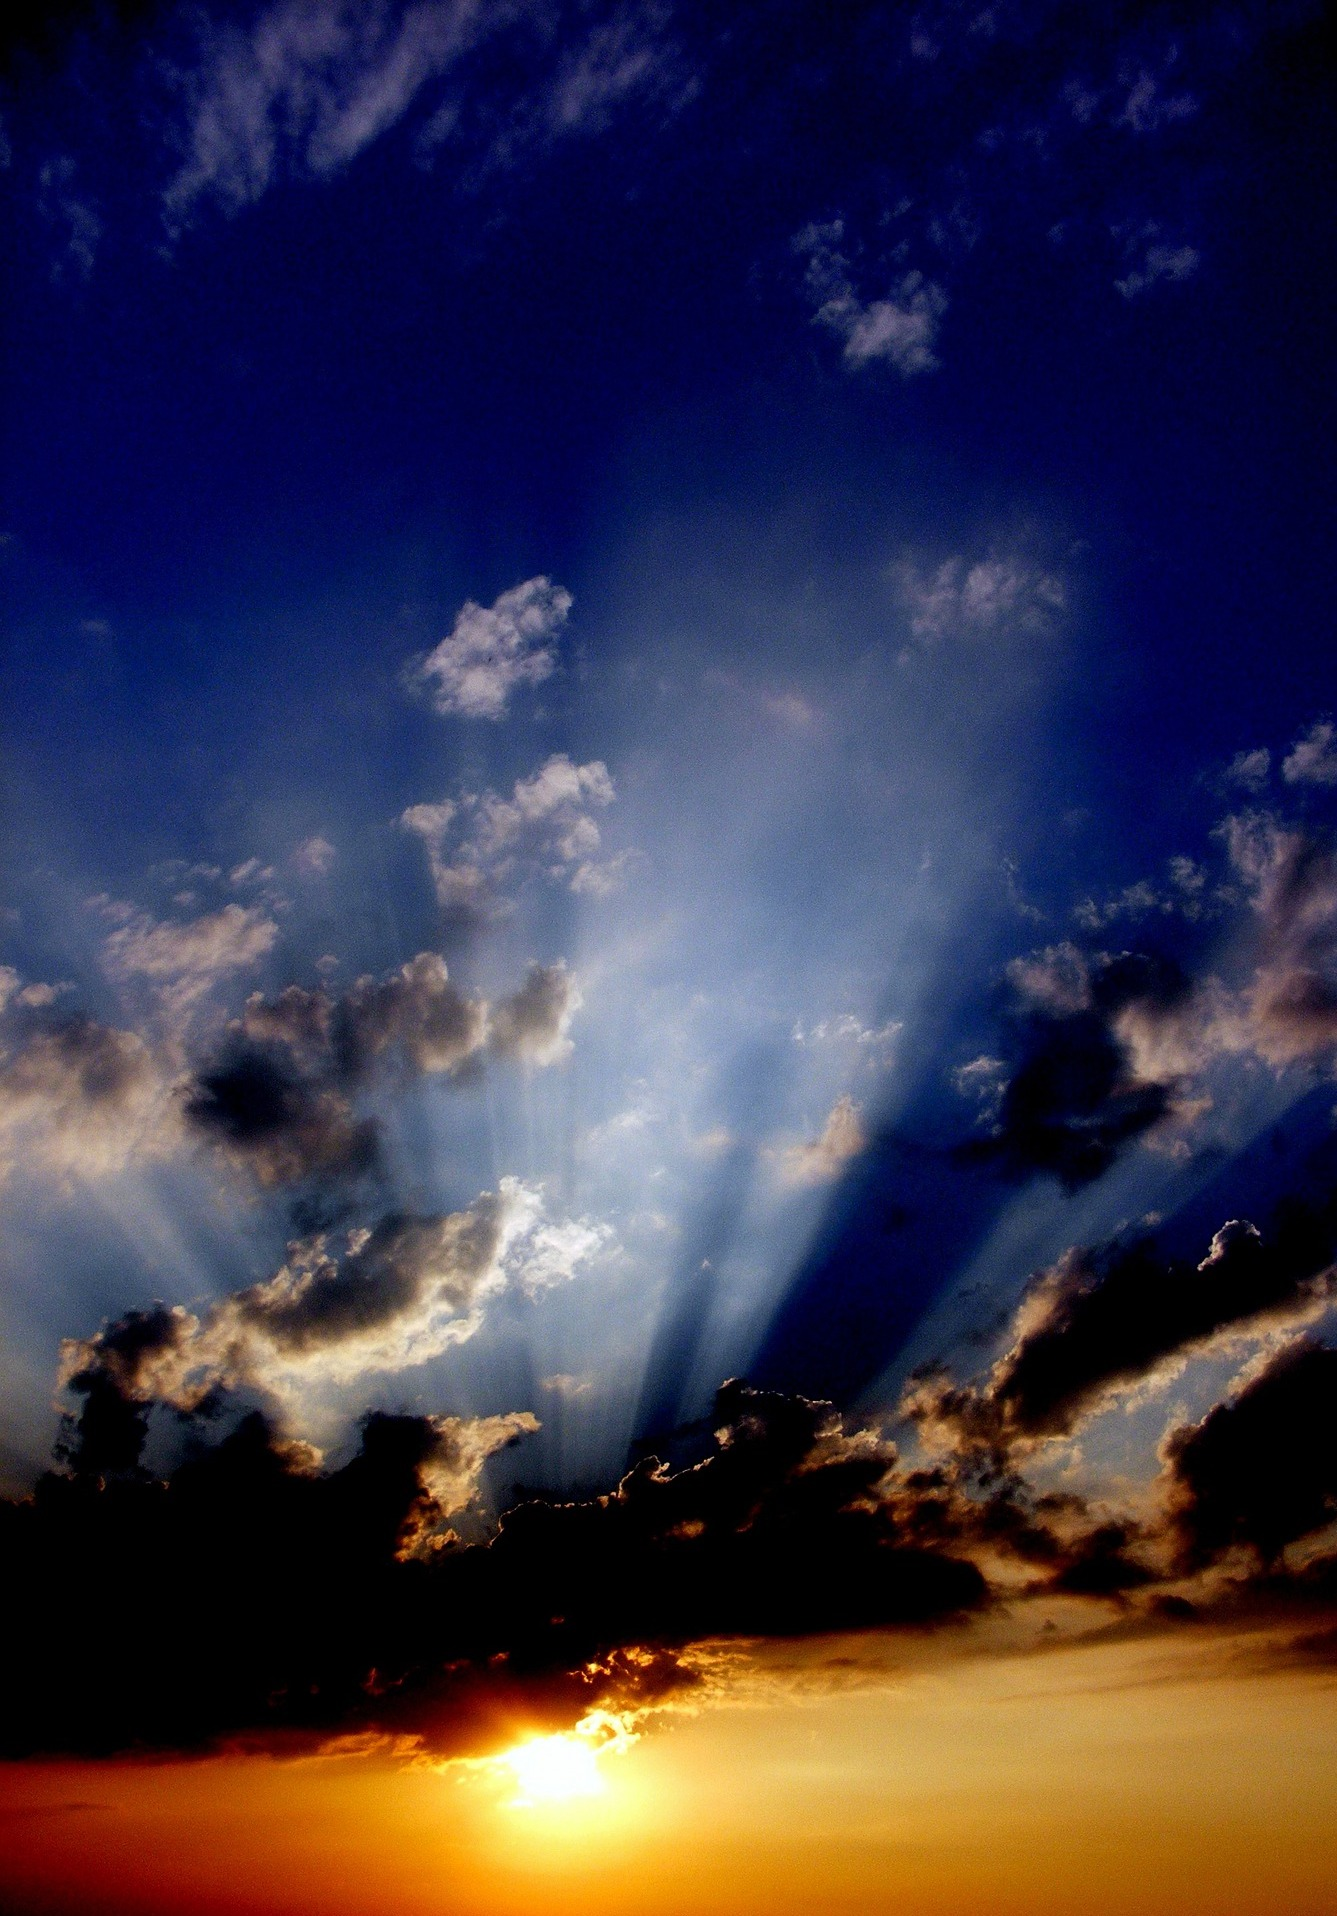
\includegraphics[width=\paperwidth]{background.jpg}}; % Background image
\draw[anchor=north] (midpoint) node [fill=ocre!30!white,fill opacity=0.6,text opacity=1,inner sep=1cm]{\Huge\centering\bfseries\sffamily\parbox[c][][t]{\paperwidth}{\centering \TITLE\\[15pt] % Book title
{\Large \SUBTITLE}\\[20pt] % Subtitle
{\huge \AUTHOR}}}; % Author name
\end{tikzpicture}};
\end{tikzpicture}
\vfill
\endgroup


%----------------------------------------------------------------------------------------
%	COPYRIGHT PAGE
%----------------------------------------------------------------------------------------

\newpage
~\vfill
\thispagestyle{empty}

\noindent Copyright \copyright\ 2016 Gregor von Laszewski\\ % Copyright notice

\noindent \textsc{Published by Indiana University}\\ % Publisher

\noindent \textsc{https://github.com/cloudmesh/classes}\\ % URL

\noindent Licensed under the Creative Commons Attribution-NonCommercial 3.0 Unported License (the ``License''). You may not use this file except in compliance with the License. You may obtain a copy of the License at \url{http://creativecommons.org/licenses/by-nc/3.0}. Unless required by applicable law or agreed to in writing, software distributed under the License is distributed on an \textsc{``as is'' basis, without warranties or conditions of any kind}, either express or implied. See the License for the specific language governing permissions and limitations under the License.\\ % License information

\noindent \textit{First printing, January 2017} % Printing/edition date

%----------------------------------------------------------------------------------------
%	TABLE OF CONTENTS
%----------------------------------------------------------------------------------------

%\usechapterimagefalse % If you don't want to include a chapter image, use this to toggle images off - it can be enabled later with \usechapterimagetrue

\chapterimage{matrix.jpg} % Table of contents heading image

\pagestyle{empty} % No headers

\tableofcontents % Print the table of contents itself

\cleardoublepage % Forces the first chapter to start on an odd page so it's on the right

\pagestyle{fancy} % Print headers again

%----------------------------------------------------------------------------------------




\chapter{I524 Preface}
\label{\detokenize{notes:i524-notes}}\label{\detokenize{notes:i524-preface}}

\section{Preface}
\label{\detokenize{i524/preface/index::doc}}\label{\detokenize{i524/preface/index:preface}}

\subsection{About}
\label{\detokenize{i524/preface/about:about}}\label{\detokenize{i524/preface/about::doc}}
This Web page is hosted at
\begin{itemize}
\item {} 
\url{https://cloudmesh.github.io/classes/}

\end{itemize}

The Piazza group is available at:
\begin{itemize}
\item {} 
\url{https://piazza.com/class/ix39m27czn5uw}

\end{itemize}

The PDF version of a \sphinxstylestrong{subset} if the information posted on the Web
page is located at:
\begin{itemize}
\item {} 
\url{https://cloudmesh.github.io/classes/i524-notes.pdf}

\end{itemize}

This PDF document will be updated on a weekly basis and we will
integrate what we have taught you in class and serve as lecture notes.
However do not forget a lot of information is on teh Web Page and in
piazza. So these PDF notes will not be sufficient for you for this
class.


\subsection{Disclaimer}
\label{\detokenize{i524/preface/disclaimer::doc}}\label{\detokenize{i524/preface/disclaimer:disclaimer}}
It is normal that questions posed by the students in the
online and residential classes lead to improvements and clarifications
of the content published on the class Web pages. Hence you need to
revisit the page updates. Just as in other years we provide a
changelog. Changes will not lead to any requirements change to the class
but only improving the content. However, we have learned from previous
classes that additional homework may need to be added in case the
class participants need to grasp a concept better or simplify their
work.

We have two ways of providing content to the class:
\begin{itemize}
\item {} 
we release content only on weekly basis

\item {} 
we release content even in draft form

\end{itemize}

We decided to do the later so you may have the ability to see what is
comming up. Please do not mistake this as a changing requirement. This
is an opportunity for you. You are not required to look at lectures or
assignments that are not yet released for this class.


\subsection{Conventions}
\label{\detokenize{i524/preface/convention::doc}}\label{\detokenize{i524/preface/convention:conventions}}\begin{description}
\item[{\sphinxtitleref{\$}}] \leavevmode
When showing examples of commands, the \sphinxtitleref{\$} symbol precedes the
actual command. So, the other lines are the output obtained after
executing the command. An example invoking the ls command
follows:

\begin{sphinxVerbatim}[commandchars=\\\{\}]
\PYGZdl{} ls
\end{sphinxVerbatim}

\item[{\sphinxtitleref{PORTALNAME}}] \leavevmode
In some examples we refer to your portal name as the \sphinxtitleref{PORTALNAME}
you have on FutureSystems.

\item[{\sphinxtitleref{USERNAME}}] \leavevmode
In some examples we refer to your local computers name as
\sphinxtitleref{USERNAME}. Your portal name and your local name may be
different.

\item[{Menu selections:}] \leavevmode
\sphinxtitleref{Start --\textgreater{} Programs}

\item[{Man page:}] \leavevmode
\sphinxstyleemphasis{ls(1)}

\end{description}


\subsection{Instructors}
\label{\detokenize{i524/preface/instructors:instructors}}\label{\detokenize{i524/preface/instructors::doc}}
The course presents lectures in online form given by the instructors
listed bellow. Many others have helped making this material available
and may not be listed here. For this class support is provided by
\begin{itemize}
\item {} 
Gregor von Laszewski (PhD)

\item {} 
Badi' Abdul-Wahid (PhD)

\item {} 
Jerome Mitchell (Teaching Assistant)

\item {} 
Miao Zhang (Teaching Assistant)

\item {} 
Tony Liu (Teaching Assistant)

\item {} 
Vibhatha Abeykoon (Teaching Assistant)

\item {} 
Dimitar Nikolov (Teaching Assistant)

\end{itemize}


\subsubsection{Dr. Gregor von Laszewski}
\label{\detokenize{i524/preface/instructors:dr-gregor-von-laszewski}}
\noindent\sphinxincludegraphics{{gregor22}.png}

Gregor von Laszewski is an Assistant Director of Cloud Computing in
the DSC. His is also an Adj. Assoc. Professor of the Intelligent
Systems Engineering Department at Indiana University. He held a
position at Argonne National Laboratory from Nov. 1996 \textendash{} Aug.  2009
where he was last a scientist and a fellow of the Computation
Institute at University of Chicago. During the last two years of that
appointment he was on sabbatical and held a position as Associate
Professor and the Director of a Lab at Rochester Institute of
Technology focussing on Cyberinfrastructure. He received a Masters
Degree in 1990 from the University of Bonn, Germany, and a Ph.D. in
1996 from Syracuse University in computer science. He was involved in
Grid computing since the term was coined. He was the lead of the Java
Commodity Grid Kit (\url{http://www.cogkit.org}) which provides till today a
basis for many Grid related projects including the Globus
toolkit. Current research interests are in the areas of Cloud
computing. He is leading the effort to develop a simple IaaS client
available at as OpenSource project at
\url{http://cloudmesh.github.io/client/}

His Web page is located at \url{http://gregor.cyberaide.org}. To contact him
please send mail to \href{mailto:laszewski@gmail.com}{laszewski@gmail.com}. For class related e-mail
please use Piazza for this class.

In his free time he teaches Lego Robotics to high school students. In 2015
the team won the 2nd prize in programming design in Indiana. If you like
to volunteer helping in this effort please contact him.

He offers also the opportunity to work with him on interesting
independent studies. Current topics include but are not limited to
\begin{itemize}
\item {} 
cloudmesh

\item {} 
big data for NIST

\item {} 
big data benchmarking.

\item {} 
scientific impact of supercomputer and data centers.

\item {} 
STEM and other educational activities while using robotics or big data

\end{itemize}

Please contact me if you are interested in this.


\subsubsection{Dr. Geoffrey C. Fox}
\label{\detokenize{i524/preface/instructors:dr-geoffrey-c-fox}}
\noindent\sphinxincludegraphics{{gcf2}.jpg}

Greoffrey C. Fox received a Ph.D. in Theoretical Physics from Cambridge University
and is now distinguished professor of Informatics and Computing, and
Physics at Indiana University where he is director of the Digital
Science Center, Chair of Department of Intelligent Systems Engineering
and Director of the Data Science program at the School of Informatics
and Computing.  He previously held positions at Caltech, Syracuse
University and Florida State University after being a postdoc at the
Institute of Advanced Study at Princeton, Lawrence Berkeley Laboratory
and Peterhouse College Cambridge. He has supervised the PhD of 68
students and published around 1200 papers in physics and computer
science with an index of 70 and over 26000 citations.  He currently
works in applying computer science from infrastructure to analytics in
Biology, Pathology, Sensor Clouds, Earthquake and Ice-sheet Science,
Image processing, Deep Learning, Manufacturing, Network Science and
Particle Physics. The infrastructure work is built around Software
Defined Systems on Clouds and Clusters. The analytics focuses on
scalable parallelism.

He is involved in several projects to enhance the capabilities of
Minority Serving Institutions. He has experience in online education
and its use in MOOCs for areas like Data and Computational Science. He
is a Fellow of APS (Physics) and ACM (Computing).


\subsubsection{Dr. Badi' Abdul-Wahid}
\label{\detokenize{i524/preface/instructors:dr-badi-abdul-wahid}}
\noindent\sphinxincludegraphics{{badi2}.png}

Badi' received a Ph.D. in Computer Science at the University of Notre
Dame under Professor Jesus Izaguirre. The primary focus of his
graduate work was the development of scalable, fault-tolerant, elastic
distributed applications for running Molecular Dynamics simulations.

At Indiana University, Badi' works with the FutureSystems project
on a NIST-funded study whose goal is to understand patterns in the
development and usage of Big Data Analysis pipelines.


\subsection{Teaching Assistants}
\label{\detokenize{i524/preface/instructors:teaching-assistants}}

\subsubsection{Jerome Mitchell}
\label{\detokenize{i524/preface/instructors:jerome-mitchell}}
\noindent\sphinxincludegraphics{{jerome2}.png}

\sphinxstylestrong{Jerome Mitchell} is a Ph.D candidate in computer science at Indiana
University and is interested in coupling the fields of computer and
polar science. He has participated in the United State Antarctic
Program, (USAP), where he collaborated with a multidisciplinary team
of engineers and scientists to design a mobile robot for harsh polar
environments to autonomously collect ice sheet data, decrease the
human footprint of polar expeditions, and enhance measurement
precision. His current work include: using machine learning techniques
to help polar scientists identify bedrock and internal layers in radar
imagery. He has also been involved in facilitating workshops to
educate faculty and students on the importance of parallel and
distributed computing at minority-serving institutions.


\subsubsection{Dimitar Nikolov}
\label{\detokenize{i524/preface/instructors:dimitar-nikolov}}
\noindent\sphinxincludegraphics{{dimitar}.png}

\sphinxstylestrong{Dimitar Nikolov} is a PhD student in the Computer Science program at
Indiana University since August 2008. His research interests include
online social networks, tagging systems and web mining. As part of his
PhD he conducts research with the NaN group, led by Professor Fil
Menczer. His thesis topic is TBD.


\subsubsection{Vibhatha Abeykoon}
\label{\detokenize{i524/preface/instructors:vibhatha-abeykoon}}
\noindent\sphinxincludegraphics{{vb}.png}

\sphinxstylestrong{Vibhatha Abeykoon} is a PhD student in the Intelligent Systems Engineering program at
Indiana University since August 2016. His research interests include
machine learning, singal processing, source seperation, deep learning, big data and distributed systems. As part of his
PhD he conducts research with Professor Geoffrey C. Fox and Assistant Professor Minje Kim. His thesis topic is TBD.


\subsubsection{Miao Zhang}
\label{\detokenize{i524/preface/instructors:miao-zhang}}
\noindent\sphinxincludegraphics{{miao100px}.jpg}

\sphinxstylestrong{Miao Zhang} PhD student working primarily on computer network related stuff.
Currently focuses on network performance monitoring and forecasting.


\subsubsection{Tony Liu}
\label{\detokenize{i524/preface/instructors:tony-liu}}
\noindent\sphinxincludegraphics{{tony}.png}

\sphinxstylestrong{Tony Liu} is a PhD student in the Intelligent Systems Engineering program at Indiana University since August 2016. He received his Master degree in Computer Science program in May 2016 at IU. His research interests are high performance computing, computer systems and computer architecture. He used to work under Professor Thomas Sterling and Professor Andrew Lumsdaine from Center for Research in Extreme Scale Technology (CREST) on HPX-5 runtime system project. His currently works on benchmarking Intel Xeon Phi Knights Landing processor with Caffe under Professor Judy Qiu and Professor Lei Jiang.


\chapter{I524 Introduction}
\label{\detokenize{notes:i524-introduction}}
\index{i524}

\section{i524 Overview}
\label{\detokenize{i524/index:index-0}}\label{\detokenize{i524/index::doc}}\label{\detokenize{i524/index:i524-overview}}
This course studies software used in many commercial activities
related to Big Data. The backdrop for course contains more than 370
software subsystems illustrated in Figure 1.  We will describe the
software architecture represented by this collection and work towards
identifying best practices to deploy, access and interface with
them. Topics of this class will include:

\index{I524 technology image}\begin{figure}[htbp]
\centering
\capstart

\noindent\sphinxincludegraphics{{bigdata}.png}
\caption{Big data relevant technology layers}\label{\detokenize{i524/index:id1}}\end{figure}
\begin{enumerate}
\item {} 
The cloud computing architecture underlying open source big data
software and frameworks and contrast of them to high performance
computing

\item {} 
The software architecture with its different layers covering broad
functionality and rationale for each layer.

\item {} 
We will go through selected big data stack software from the list
of more than 370

\item {} 
We will be identifying how we can create and replicate software
environments based on software deployed and used on clouds while
using Containers, OpenStack and Ansible playbooks.

\item {} 
Students will chose a number of open source members of the list
each and create repeatable deployments as illustrated in class.

\item {} 
The main activity of the course will be building a significant
project using multiple subsystems combined with user code and
data. Projects will be suggested or students can chose their own. A
project report will summarize the work conducted.

\item {} 
Topics taught in this class will be very relevant for industry as
you are not only exposed to big data, but you will also be
practically exposed to DevOps and collaborative code development
tools as part of your homework and project assignment.

\end{enumerate}

Students of this class will need to conduct their project deployments
in python using ansible and enabling a software stack that is useful
for a big data analysis. While it is not necessary to know either
python or ansible to take the class it is important that you have
knowledge of a programming language so you can enhance your knowledge
on them throughout the class and succeed. You will be expected to have
a computer on which you have python 2.7.x installed.  You will be
using chameleon and possibly our local cloud. Optionally some projects
may use docker.

Figure 2 illustrates that you can follow the components of the class
in a variety of ways and in parallel. For example, you do not have to
wait to start the project or to find out more about any of the
subsystems.

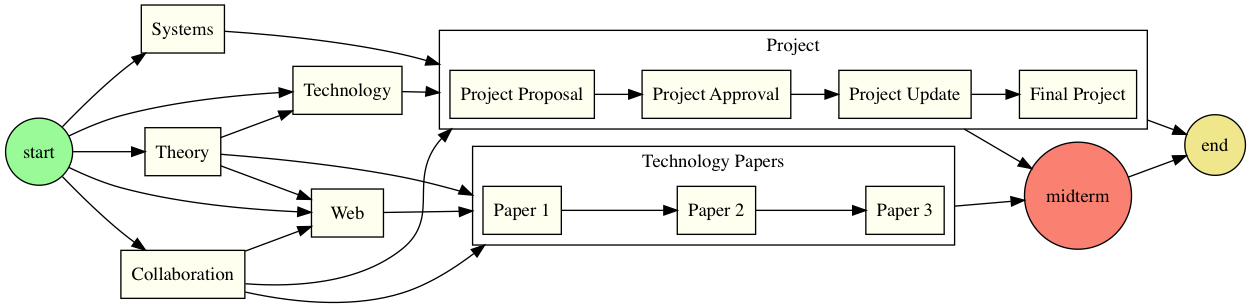
\includegraphics{graphviz-4a0f061ade3cfd06c3793cabb8f3282d54e0a835.pdf}

\sphinxstylestrong{Figure 2:} Components of the Class

\begin{sphinxadmonition}{note}{Note:}
You do not have to take I523 in order to take I524.

\sphinxstylestrong{For previous I523 class participants:} While I523 is a
beginners class I524 is a more advanced class and we expect that
you know python which you hopefully have learned as part of
I523 while doing a software project. If not, make sure you
learn it before you take this class or consider
\sphinxstylestrong{significant} additional time needed to learn it for the
class.

\sphinxstylestrong{Residential students need to enroll early} so we avoid the
situation like last year where we had many signing up, but
did not even show up to the first lecture. I have asked that
students from I523 have preference, but I am not sure if we
can enforce this. So enroll ASAP. Those that are on the
waiting list are recommended to show up in the first
class. It is likely that you can join as others drop.
\end{sphinxadmonition}

\index{I524 meeting times}

\subsection{Meeting Times}
\label{\detokenize{i524/index:meeting-times}}\label{\detokenize{i524/index:index-2}}
The classes are published online. Residential students at Indiana
University will participate in a discussion taking place at the
following time:
\begin{itemize}
\item {} 
Monday 09:30am - 10:45am EST, I2 130

\end{itemize}

For the 100\% online students see the office hours.


\subsection{Online Meetings}
\label{\detokenize{i524/index:online-meetings}}
For the zoom information please go to

\url{https://iu.instructure.com/courses/1603897/assignments/syllabus}

A doodle was used and all students that answered the doodle have times
that they specified. We covered 100\% the time for the students through
the following schedule:

All times are in Eastern Standard Time.

\noindent\begin{tabular}{|*{2}{p{\dimexpr(\linewidth-\arrayrulewidth)/2-2\tabcolsep-\arrayrulewidth\relax}|}}
\hline

\sphinxstylestrong{Day of Week}
&
\sphinxstylestrong{Meetings}
\\
\hline
Monday
&
\begin{DUlineblock}{0em}
\item[] 8-9am Office Hours
\item[] 9:30-10:45am Residential Lecture
\item[] 6-7pm Office Hours
\end{DUlineblock}
\\
\hline
Tuesday
&
\begin{DUlineblock}{0em}
\item[] 1-2pm Office Hours
\item[] 4-5pm Office Hours
\end{DUlineblock}
\\
\hline
Wednesday
&
6-7pm Office Hours
\\
\hline
Thursday
&
6-7pm Office Hours (Gregor)
\\
\hline
Friday
&
4-5pm Office Hours
\\
\hline
Saturday
&
8-9pm Office Hours
\\
\hline
Sunday
&
\begin{DUlineblock}{0em}
\item[] 9-10am Office Hours
\item[] 8-9pm Office Hours
\end{DUlineblock}
\\
\hline\end{tabular}



\subsection{Who can take the class?}
\label{\detokenize{i524/index:who-can-take-the-class}}\begin{itemize}
\item {} 
Although Undergrads can take this class it will be thaught as
graduate class. Make sure you have enough time and fulfill the
prerequisites such as knowing a programming language well. You need
to have enough time to learn python if you do not know it.

\item {} 
You can take I524 without taking I523, but you must be proficient
in python. Overlap between I523 and I524 only relates to some
introduction lectures and naturally lectures from the systems track
such as github, report writing, introduction to python.

\item {} 
Online students

\item {} 
Residential students

\end{itemize}


\subsection{Homework}
\label{\detokenize{i524/index:homework}}
\index{I524 homework}
Grading policies are listed in Table 1.


\begin{threeparttable}
\capstart\caption{Table 1: Grading}\label{\detokenize{i524/index:id2}}
\noindent\begin{tabulary}{\linewidth}{|L|L|}
\hline
\sphinxstylethead{\relax 
Percent
\unskip}\relax &\sphinxstylethead{\relax 
Description
\unskip}\relax \\
\hline
10\%
&
Class participation and contribution to Web pages.
\\
\hline
30\%
&
Three unique technology papers per student of the 370
systems. Each paper as at least 2 pages per technology without
references.
\\
\hline
60\%
&
Project code and report with at least 6 pages without
references. Much shorter reports will be returned without
review. Do not artificially inflate contents.
\\
\hline\end{tabulary}

\end{threeparttable}

\begin{itemize}
\item {} 
\sphinxstylestrong{Technology papers:} Technology papers must be non-overlapping in
the entire class. As we have over 370 such technologies we should
have enough for the entire class. If you see technologies missing,
let us know and we see how to add them. Technology papers could be a
survey of multiple technologies or an indepth analysis of a
particular technology.

\item {} 
\sphinxstylestrong{Technology paper groups:} Groups of up to three students can work
also on the technology papers. However the workload is not reduced,
you will produce 3 times the number of group members technology
papers of unique technologies. However, you can have multiple
coauthors for each paper (up to thre) that are part of your
group. Please do not ask us how many technology papers you need to
write if you are in a group. The rule is clearly specified. Example:
Your group has 3 members, each of them has to procude 3 unique
papers, thus you have to produce 9 unique technology papers for this
group. If you have 2 members you have to produce 6, if you work
alone you have to produce 3.

\item {} 
\sphinxstylestrong{Technology deployment Homework:} Each student will
develop as a preparation for the project a deployment of a
technology. Points may depend on completeness, effort of the
deployment. Technology deployments should as much as possible be non
overlapping. In many cases you chose wisely such deployments may
line up with your technology papers as you can add a section
reporting on your achievement and experience with such
deployments.

\item {} 
\sphinxstylestrong{Project groups:} Groups of up to three students can work on a
project but workload increases with each student and a work break
down must be provided.  More than three students are not allowed. If
you work in a group you will be asked to deploy a larger system or
demonstrate deployability on multiple clouds or container frameworks
while benchmarking and comparing them. A group project containing 2
or 3 team members should not look like a project done by an
individual. Please plan careful and make sure all team members
contribute.

\item {} 
\sphinxstylestrong{Frequent checkins}: It is \sphinxstylestrong{important} to make frequent and
often commits to the github repository as the activities will be
monitored and will be integrated into the project grade.  Note that
paper and project will take a considerable amount of time and doing
proper time management is a must for this class. Avoid starting your
project late. Procrastination does not pay off.

\item {} 
\sphinxstylestrong{No bonus projects:} This class will not have any bonus projects
or regrading requests. Instead you need to focus your time on the
papers and the project assignments and homework.

\item {} 
\sphinxstylestrong{Voluntary work:} You are welcome to conduct assignments and
excerises you find on the class Web page on your own. However they
are not graded or considered for extra credit.

\item {} 
\sphinxstylestrong{Late homework}: Any late homework will be receiving a 10\% grade
reduction.  As this is a large class and the assignments are not
standard multiple choice questions, grading will take a considerable
time. Some homework can not be delivered late as they are related to
establish communication with you. Such \sphinxstylestrong{deadline specific}
homework will receive 0 points in case they are late. See course
calendar. It is the student’s responsibility to upload submissions
well ahead of the deadline to avoid last minute problems with
network connectivity, browser crashes, cloud issues, etc.

\item {} 
\sphinxstylestrong{Chance for publishing a paper:} If however you find that the work
you do could lead to a publishable paper, you could work together
with the course instructor as coauthors to conduct such an
activity. However, this is going to be a significant effort and you
need to decide if you like to conduct this. In such cases if the
work is sufficient for publication submission, an A+ for the class
could be considered. It will be a lot of work. The length of such a
paper is typically 10-12 high quality pages including figures and
references. We may elect for the final submission to use a different
LaTeX style

\end{itemize}


\subsection{Prerequisites}
\label{\detokenize{i524/index:prerequisites}}\label{\detokenize{i524/index:ref-i524-prerequisits}}
\index{I524 prerequisites}
We expect you are familiar with:
\begin{itemize}
\item {} 
Linux and the Operating system on which you will focus your
deployment.

\item {} 
Note that Windows as OS will not be sufficient as Ansible
is not supported on it. However you can use virtualbox or log onto
one of the clouds to get access to an OS that supports ansible. So
you can use your Windows computer if it is powerful enough.

\item {} 
Python 2.7.x (we will not use python 3 for this class as it
is not yet portable with all systems) Although python is considered
to be a straight forward language to learn, students that have not
done any programming my find it challanging.

\item {} 
Familaiarity with th Python eco system. The best way to install
python on a computer is to use virtualenv, and pip (which we will
teach you as part of the class).

\item {} 
Familiarity with an editor such as emacs, vi, jedit, pyCharm,
eclipse, or other that you can use to program in and write your
reports.

\end{itemize}

If you are not familiar with these technologies, we expect that you
get to know them before or during class. This may pose additional time
commitment.


\subsection{Open Source Publication of Homework}
\label{\detokenize{i524/index:open-source-publication-of-homework}}
\index{I524 report format}
As this class is about open source technologies, we will be using such
technologies to gather the homework submissions. We will not be using
CANVAS so we teach you these technologies that are often mandated in
industry. CANVAS is not.

As a consequence all technology papers from all students will be
available as a single big technical report. To achieve this all
reports must be written in the same format. This wil be LaTeX and all
references have to be provided a bibtex file while you use jabref.
Alternatively lyx.org can be used, if you prefer to edit
latex in \sphinxstyleemphasis{what you see is almost what you get} format. The use of
sharelatex or overleave or lyx.org is allowed.

\index{I524 piazza}

\subsection{Piazza}
\label{\detokenize{i524/index:index-6}}\label{\detokenize{i524/index:piazza}}
All communication will be done via Piazza. We will not read e-mail
send to our university or private e-mails. All instructors are
following this rule. Any mail that is not send via Piazza will be
\sphinxstylestrong{not read} and \sphinxstylestrong{deleted}. This is also true for any mail send to
the inbox system in CANVAS. We found CANVAS a not scalable solution
for our class and will not use CANVAS for reaching out to you.   If you
need a different mechanism to communicate with us, please ask on Piazza
how to do that. Please note that private posts in piazza are shared
among all instructors and TAs.

To sign up in piazza please follow this link:
\begin{itemize}
\item {} 
\url{https://piazza.com/iu/spring2017/i524}

\end{itemize}

We have created a number of piazza folder to organize the posts int
topics.  Thes folders are:
\begin{description}
\item[{help:}] \leavevmode
Our help folder is just like a ticket system that is monitored by
the TA's. Once you file a question here, a TA will attend to it,
and work with you. Once the issue you had is resolved, the TA is
marking it as resolved. If you need to reopen a help message,
please mark it again as unresolved or post a follow up.

\item[{project:}] \leavevmode
Questions related to projects are posted here.

\item[{logistics:}] \leavevmode
Question regarding the logistics of the class are posted
here. This includes questions about communication, meeting times,
and other administrative activities.

\item[{papers:}] \leavevmode
Questions regarding the paper are posted here.

\item[{grading:}] \leavevmode
Questions regarding grades are posted here.

\item[{clouds:}] \leavevmode
Questions regarding cloud resources are posted here.

\item[{faq:}] \leavevmode
Some questions will be transformed to FAQ's that we post here.
Note also that we have an FAQ on the class Web page that you may
want to visit. We try to move important FAQ's from Piazza into the
Web page, so it is important that you check both.

\item[{meetings: Here we will post times for meetings with TA's and}] \leavevmode
instructors that are not yet posted on the Web page as part of the
regular meeting times. Class participants are allowed to attend
any Zoom meeting that we annonce in this folder. For online
students we will also determine a time for regulare meetings. The
TAs are required to hold 10 hours of meeting times upon request
with you. Please make use of this.

\item[{other:}] \leavevmode
In case no folder matches for your question use other.

\end{description}

\index{I524 tips}

\subsection{Tips on how to achieve your best}
\label{\detokenize{i524/index:tips-on-how-to-achieve-your-best}}\label{\detokenize{i524/index:index-7}}
While teaching our classes we noticed the following tips to achieve
your best:
\begin{itemize}
\item {} 
Listening to the lectures

\item {} 
\sphinxstylestrong{Set aside enough undisturbed time for the class}. Switch off
facebook, twitter, or other distracting social media systems when
focussing on the class.

\item {} 
\sphinxstylestrong{Ask for help}. The TAs can schedule custom help office hours on
appointment during reasonable times.

\item {} 
Do not \sphinxstylestrong{Procrastinate}.

\item {} 
Do not \sphinxstylestrong{take your other classes more serious}.

\item {} 
\sphinxstylestrong{Start the project in the first 4 weeks of the class}

\item {} 
Be aware that this class is not based on a text book and what this
implies.

\item {} 
Do not overestimating the technical abilities.

\item {} 
Do not underestimating the time it takes to do the project.

\item {} 
Do not forget to include benchmarks in your project.

\item {} 
Unnecessarily struggling with LaTeX as you do not use an example we
provide.

\item {} 
Trying to do things just on Windows which is typically more difficult
than using Linux.

\item {} 
Not having a computer that is up to date. Update your memory and
have a SSD

\item {} 
Ignoring obvious security rules and not integrating ssh form the
start into your projects.

\item {} 
Not posting passwords into git. For example git does
\sphinxstylestrong{not} allow to \sphinxstylestrong{easily} completely delete files that contain secret
information such as passwords. It takes significant effort to do
that. Make sure you do add in git on individual files and never
just a bulk add.

\item {} 
Having your coleagues do the work for you

\item {} 
Underestimating the \sphinxstylestrong{time} it takes to do deployments

\item {} 
Not reading our piazza posts and repeating the same question over
and over

\item {} 
Use Piazza to communicate and not CANVAS or e-mail.

\item {} 
When you receive an e-mail from piazza, reply to it while clicking
on the link instead of replying via e-mail directly. This is more
reliable.

\end{itemize}


\subsection{Submissions}
\label{\detokenize{i524/index:submissions}}
Your papers and projects will be developed on GitHub and submitted
using \DUrole{xref,doc}{Pull Requests}.  The process
is as follows:
\begin{enumerate}
\item {} 
fork the \href{https://github.com/cloudmesh/sp17-i524}{sp17-i524} repository.

\item {} 
clone your fork and commit and push your changes.

\item {} 
submit a pull request to the master branch of the origin repository.

\end{enumerate}

See the repository for details on the individual assignments. As it
will periodically be updated, make sure you are familiar with the
process of \href{https://help.github.com/articles/syncing-a-fork/}{Syncing a fork}.

Some things to keep in mind:
\begin{itemize}
\item {} 
space on github is limited, so do not add datasets to the
repository. Any datasets you use should be publicly hosted and
deployed as part of your project ansible deployment scripts.

\item {} 
never add ssh private keys to the repository. This results in a
security risk, possible point deductions, and lots of time and
effort to fix.

\item {} 
all work will be licensed under the Apache 2 open source license.

\item {} 
all submissions and discussion will be visible to the world.

\end{itemize}

\index{I524 project ideas}

\subsection{Selected Project Ideas}
\label{\detokenize{i524/index:selected-project-ideas}}\label{\detokenize{i524/index:index-8}}
Students can select from a number of project ideas. We will improve
and add additional ideas throughout the semester. Students can also
conduct their own projects. We recommend that you identify a project
idea by the end of the first month of the class. Example project
descriptions that you may want to take a look at include:
\begin{itemize}
\item {} 
\DUrole{xref,std,std-ref}{robotswarm}

\item {} 
\DUrole{xref,std,std-ref}{dockerswarm}

\item {} 
\DUrole{xref,std,std-ref}{kubernetes}

\item {} 
\DUrole{xref,std,std-ref}{slurmcluster}

\item {} 
\DUrole{xref,std,std-ref}{authordisambiguity\_b}

\item {} 
NIST Big Data Working group examples: Selected and approved use case from
\url{http://nvlpubs.nist.gov/nistpubs/SpecialPublications/NIST.SP.1500-3.pdf}

\item {} 
Selected examples from Fall I523:
Some students may have created an example as part of I523. Not all
examples created as part of this class qualify for a I524
project. Please contact Gregor von Laszewski via Piazza to discuss
suitability of your previous I523 project. If such a project is
selected, approved and used it is expected it is significantly
enhanced.

\item {} 
Cloudmesh Enhancements:
A number of projects could center around the enhancements of
cloudmesh for the improvement of big data projects using virtual
machines and containers. This includes:
\begin{itemize}
\item {} 
Development of REST services for cloudmesh while using cloudmesh
client

\item {} 
Development of benchmarking examples while using cloudmesh client

\item {} 
Development of a better Azure interface to additinal services

\item {} 
Development of a better AWS interfac to additinal services

\item {} 
Development of a Web interface while using django

\item {} 
SLURM integration to create virtual clusters on comet

\item {} 
Port cloudmesh client to Windows 10

\item {} 
Integrate docker into cloudmesh and demonstrate its use

\item {} 
Integrate kubernetes into cloudmesh and demonstrate its use

\item {} 
Expand the HPC capabilities of cloudmesh

\end{itemize}

\end{itemize}


\subsection{Software Project}
\label{\detokenize{i524/index:software-project}}
For a software project you have the choice of working indifidualy or
working in a team of up to three students. You can use the \sphinxstylestrong{search
teammate} folder to find and form groups:
\begin{itemize}
\item {} 
\url{https://piazza.com/class/ix39m27czn5uw?cid=5}

\end{itemize}

The following artifacts are part of the deliverables for a project
\begin{description}
\item[{Code:}] \leavevmode
You must deliver the code in github. The code must be compilable
and a TA may try to replicate to run your code. You MUST avoid
lengthy install descriptions and everything must be installable
from the command line. We will check submission. All team members
must be responsible for one part of the project.

\item[{Project Report:}] \leavevmode
A report must be produced while using the format discussed in the
Report Format section. The following length is required:
\begin{itemize}
\item {} 
4 pages, one student in the project

\item {} 
6 pages, two students in the project

\item {} 
8 pages, three students in the project

\end{itemize}

\item[{Work Breakdown:}] \leavevmode
The report contains in an appendix a section that is
only needed for team projects. Include in the section a short but
sufficiently detailed work breakdown documenting what the team has
done. Back it up with commit information from github. Such as how
many commits and lines of code a team member has contributed. The
section does not count towards the overall length of the paper.

In addition the graders will check the history of checkins to
verify each team member has used github to checkin their
contributions frequently. E.g. if we find that one of the students
has not checked in code or documentation in the same way at other
teammates, it will be questioned. An oral exam may be scheduled to
verify that the student has contributed to the project. In an oral
exam the student must be familiar with \sphinxstylestrong{all} aspects of the
project not just the part you contributed.

\item[{License:}] \leavevmode
All projects are developed under an open source license such
as Apache 2.0 License. You will be required to add a LICENCE.txt
file and if you use other software identify how it can be reused
in your project. If your project uses different licenses, please
add in a README.md file which packages are used and which license
these packages have while adding a licenses file.

\item[{Reproducability:}] \leavevmode
The reproducability of your code will be tested
twice. It is tetes by another student or team, it is also tested
by a TA. A report of the testing team is provided. Your team will
also be responsible for executing as many tests as you have team
members on other projects. A reproducability statement should be
written with details about functionality, readbility, and report
quality. This statement does not have to be written in latex but
uses RST.

\item[{Requirements:}] \leavevmode\begin{itemize}
\item {} 
Use of cloud resources mandatory, can be substituted by
kubeernetes or docker swarm

\item {} 
Deployment must be done with ansible

\item {} 
A Makefile or a cmd file as discussed in class is needed to
deploy the software, start the program, conduct a
parameter study/benchmark

\item {} 
Report

\item {} 
If project is conducted in a team at least two clouds are to be
benchmarked and contrasted 2 team members = 2 clouds, 3 team
members = 3 clouds. cloud could also be kubernetes or docker
swarm

\item {} 
Cloudmesh client is to be used to start the virtual cluster in
order to avoid reinventing the wheel

\item {} 
Cloudmesh contains deployments for hadoop and spark. If these
technologies are used, it has to be shown that if the student(s)
elect to write a new ansible script for it that it is better
than the once provided by cloudmesh. Proof is to be provided by
reproducible benchmarks. If this can not be achieved the
student(s) have to write an additional ansible script for a
technologie listed in class or approved by the professor.

\end{itemize}

\item[{Additional links form another class:}] \leavevmode
This other class contains a section deployment
projects that may inspire you. You can look at suggestions and
conduct them, the rules
listed under requirements above applies: e.g. deployment must be
done in ansible and it must be done on a cloud, kubernetes, or
docker swarm. I524 will not focus on analytics. However you still
are able to do that, but it still must contain a deployment
portion.
\begin{itemize}
\item {} 
\DUrole{xref,std,std-ref}{projects}

\end{itemize}

\end{description}


\subsection{Report Format}
\label{\detokenize{i524/index:report-format}}
All reports will be using the format specified in Section {\hyperref[\detokenize{lesson/doc/report:reports}]{\sphinxcrossref{\DUrole{std,std-ref}{Report Format}}}}.

There will be \sphinxstylestrong{NO EXCEPTION} to this format. Documents not following
this format and are not professionally looking, will be returned
without review.


\subsection{Github repositories}
\label{\detokenize{i524/index:github-repositories}}
Class content repository: \url{https://github.com/cloudmesh/classes}

Class homework repository: \url{https://github.com/cloudmesh/sp17-i524}


\subsection{Code Repositories Deliverables}
\label{\detokenize{i524/index:code-repositories-deliverables}}
Code repositories are for code, if you have additional libraries or
data that are needed you need to develop a script or use a DevOps
framework to install such software. They \sphinxstylestrong{must} not be checked into
github. Thus zip files and .class, .o, precompiled python, .exe, core
dumps, and other such files files are not permissible in the
project. If we find such files you will get a 20\% deduction in your
grade. Each project must be reproducible with a simple script. An
example is:

\begin{sphinxVerbatim}[commandchars=\\\{\}]
\PYG{n}{git} \PYG{n}{clone} \PYG{o}{.}\PYG{o}{.}\PYG{o}{.}\PYG{o}{.}
\PYG{n}{make} \PYG{n}{install}
\PYG{n}{make} \PYG{n}{run}
\PYG{n}{make} \PYG{n}{view}
\end{sphinxVerbatim}

Which would use a simple make file to install, run, and view the
results. Naturally you can use ansible or shell scripts. It is not
permissible to use GUI based DevOps preinstalled frameworks (such as
the one you may have installed in your company or as part of another
project). Everything must be installable form the command line.


\subsection{Learning Outcomes}
\label{\detokenize{i524/index:learning-outcomes}}
Students will
\begin{enumerate}
\item {} 
gain broad understanding of Big Data applications and open source
technologies supporting them.

\item {} 
have intense programming experience in Python and ansible and DevOps.

\item {} 
use open source technologies to manage code in large groups of
individuals.

\item {} 
be able to communicate reserach in professional scientific reports.

\end{enumerate}

Outcome 1 is supported by a series of lectures around open source
technologies for big data.

Outcome 2 is supported by a significant software project that will
take up a considerable amount of time to plan and execute.

Outcome 1 and 4 is supported by writing 3 technology papers and a project
report that is shared with all students. Students can gain additional
insight from reading and reviewing other students contributions.

Outcome 3 is supported by using piazza and github as well as
contributiong to the class Web page with git pull requests.


\subsection{Academic Integrity Policy}
\label{\detokenize{i524/index:academic-integrity-policy}}
We take academic integrity very seriously. You are required to abide
by the Indiana University policy on academic integrity, as described
in the Code of Student Rights, Responsibilities, and Conduct, as well
as the Computer Science Statement on Academic Integrity
(\url{http://www.soic.indiana.edu/doc/graduate/graduate-forms/Academic-Integrity-Guideline-FINAL-2015.pdf}). It
is your responsibility to understand these policies. Briefly
summarized, the work you submit for course assignments, projects,
quizzes, and exams must be your own or that of your group, if group
work is permitted. You may use the ideas of others but you must give
proper credit. You may discuss assignments with other students but you
must acknowledge them in the reference section according to scholarly
citation rules. Please also make sure that you know how to not
plagiarize text from other sources while reviewing citation rules.

We will respond to acts of plagiarism and academic misconduct
according to university policy. Sanctions typically involve a grade of
0 for the assignment in question and/or a grade of F in the course. In
addition, University policy requires us to report the incident to the
Dean of Students, who may apply additional sanctions, including
expulsion from the university.

Students agree that by taking this course, papers and source code
submitted to us may be subject to textual similarity review, for
example by Turnitin.com. These submissions may be included as source
documents in reference databases for the purpose of detecting
plagiarism of such papers or codes.

It is not acceptable to use for pay services to conduct your project.
Please be aware that we monitor such services and have TAs speaking
various languages and know about these services even in different
countries. Also do not just translate a report written by someone in a
different language and claim it to be your project.


\subsection{Links}
\label{\detokenize{i524/index:links}}
This page is conveniently managed with git. The location for the
changes can be found at
\begin{itemize}
\item {} 
\url{https://cloudmesh.github.io/classes/}

\end{itemize}

The repository is at
\begin{itemize}
\item {} 
\url{https://github.com/cloudmesh/classes}

\end{itemize}

Issues can be submitted at
\begin{itemize}
\item {} 
\url{https://github.com/cloudmesh/classes/issues}

\end{itemize}

Or better use piazza so you notify us in our discussion lists.
\begin{itemize}
\item {} 
\url{https://piazza.com/iu/i524}

\end{itemize}

If you detect errors, you could also create a merge request at
\begin{itemize}
\item {} 
\url{https://github.com/cloudmesh/classes}

\end{itemize}


\subsection{Course Numbers}
\label{\detokenize{i524/index:course-numbers}}
This course is offered for Graduate (and Undergraduate students with
permission) at Indiana University and as an online course. To
Register, for University credit please go to:
\begin{itemize}
\item {} 
\url{http://registrar.indiana.edu/browser/soc4172/INFO/INFO-I524.shtml}

\item {} 
\url{http://registrar.indiana.edu/browser/soc4172/ENGR/ENGR-E599.shtml}

\end{itemize}

Please, select the course that is most suitable for your program:

\begin{sphinxVerbatim}[commandchars=\\\{\}]
INFO\PYGZhy{}I 524  BIG DATA SOFTWARE AND PROJECTS (3 CR)    Von Laszewski G
         Above class open to graduates only
         Above class taught online
         Discussion (DIS)
      30672 RSTR     09:30A\PYGZhy{}10:45A   M      I2 130    Von Laszewski G
         Above class meets with ENGR\PYGZhy{}E 599
INFO\PYGZhy{}I 524  BIG DATA SOFTWARE AND PROJECTS (3 CR)
      30673 RSTR     ARR             ARR    ARR       Von Laszewski G
         Above class open to graduates only
         This is a 100\PYGZpc{} online class taught by IU Bloomington. No
         on\PYGZhy{}campus class meetings are required. A distance education
         fee may apply; check your campus bursar website for more
         information

 ENGR\PYGZhy{}E 599  TOPICS IN INTELL SYS ENGINEER (3 CR)
       VT: BIG DATA SOFTWARE AND PROJECTS
          ***** RSTR     ARR             ARR    ARR       Von Laszewski G
             Discussion (DIS)
       VT: BIG DATA SOFTWARE AND PROJECTS
          33924 RSTR     09:30A\PYGZhy{}10:45A   M      I2 130    Von Laszewski G
             Above class meets with INFO\PYGZhy{}I 524
\end{sphinxVerbatim}


\subsection{References}
\label{\detokenize{i524/index:references}}
\url{http://hpc-abds.org/kaleidoscope/}

\index{I524 calendar}

\section{I524 Calendar}
\label{\detokenize{i524/calendar:index-0}}\label{\detokenize{i524/calendar::doc}}\label{\detokenize{i524/calendar:i524-calendar}}
\begin{sphinxadmonition}{warning}{Warning:}
This calendar may be updated based on experience from the class.
Please check back here.
\end{sphinxadmonition}

Residential classes meet Mondays 09:30A-10:45A, I2 130

\noindent\begin{tabulary}{\linewidth}{|L|L|L|}
\hline

\sphinxstylestrong{Description}
&
\sphinxstylestrong{Date/Due Dates}
&
No
\\
\hline
Class Begins
&
Mon, Jan 9
&\\
\hline
Assignment of HID
&
Fri, Jan 13
&\\
\hline
Piazza access verified  (HD)
&
Mon, Jan 16, 9am
&
C1
\\
\hline
\href{https://iu.instructure.com/courses/1603897/quizzes}{Surveys} (HD)
&
Mon, Jan 16, 9am
&
C2
\\
\hline
MLK Jr. Day.
Good time for additional class work
&
Mon, Jan 16
&\\
\hline
Github access (needed for TechList)
&
Mon, Jan 30, 9am
&
C3
\\
\hline
Acces and use of cloud verified        (HD)
&
Mon, Jan 30, 9am
&
C4
\\
\hline
Acces to python 2.7.x verified         (HD)
&
Mon, Jan 30, 9am
&
C5
\\
\hline
Access to Chameleon Cloud (see piazza)
&
Mon, Jan 30, 9am
&
C5
\\
\hline
{\hyperref[\detokenize{i524/technologies:techs-exercise}]{\sphinxcrossref{\DUrole{std,std-ref}{TechList.1a - 1.c}}}}
&
Mon, Feb 15, 9am
&
T0a
\\
\hline
\DUrole{xref,doc}{Technology Paper 1}
&
Mon, Feb 27, 9am
&
T1
\\
\hline
\DUrole{xref,doc}{BibTeX open discussions on Piazza}
&
Overdue
&
T0c
\\
\hline
Review/fixes of \DUrole{xref,doc}{BibTex open discussion on Piazza}
&
Mon, Feb 27, 9am
&
T0c
\\
\hline
{\hyperref[\detokenize{i524/technologies:techs-exercise}]{\sphinxcrossref{\DUrole{std,std-ref}{TechList.1d and Techlist 2}}}}
&
Mon, Feb 27, 9am
&
T0b
\\
\hline
{\hyperref[\detokenize{i524/python-homework::doc}]{\sphinxcrossref{\DUrole{doc}{Python cmd homework}}}}
&
See assignment link
&
T0d
\\
\hline
\DUrole{xref,doc}{TechList Peer Review}
&
See assignment link
&
T0d
\\
\hline
Technology Paper 2 due
&
Mon, Mar 27, 9am
&
T3
\\
\hline
\DUrole{xref,doc}{Ansible Deployment of Technology (New)}
&
Mon, Mar 27, 9am
&
A1
\\
\hline
Auto Witdraw
&
Sun, Mar 12
&\\
\hline
Project Execution plan and draft due   (HD)
&
Mon, Mar 13, 9am
&
P1
\\
\hline
Spring Break.
Good time for additional class work
&
Mar 12 - Mar 19
&\\
\hline
Project Updates due                    (HD)
&
Mon, Mar 27, 9am
&
P2
\\
\hline
Project due
&
Mon, Apr 24, 9am
&
P3
\\
\hline
Last day to submit late Homework
&
May 1
&\\
\hline
Ends
&
Fri, May 5
&\\
\hline\end{tabulary}

\begin{itemize}
\item {} 
(HD) hard deadlines must be done in order to obtain full
points. These deadlines are important to assure you have access to
the resources for the class.

\item {} 
Programming of A! can be substituted by a Paper 3

\end{itemize}


\subsection{Comments}
\label{\detokenize{i524/calendar:comments}}\begin{itemize}
\item {} 
Any late homework will have an automatic 10\% grade deduction.

\item {} 
Any late homework may result in substential delay in grading (one month or
more).

\item {} 
Hard deadlines can not receive any points for late submissions as they are
essential to the communication and operation of the class. If you can naturally
not communicate with we can not review your work or you can not even
execute your work.

\item {} 
Experience shows that those using additional time during the spring break do
typically better. We recommend that you use this time wisely.

\item {} 
You can start earlier if you like to prepare for this class, to for example
learn Python and ansible. However, lectures may change.

\item {} 
It would be a mistke not to start working on your project by
February 1st. You will run out of time. In order to accomodate for
this we have segnificantly reduced other homework requirements in
contrast to previous classes we taught.

\end{itemize}


\subsection{Official University calendar}
\label{\detokenize{i524/calendar:official-university-calendar}}\begin{itemize}
\item {} 
\url{http://registrar.indiana.edu/official-calendar/official-calendar-spring.shtml}

\end{itemize}


\section{I524 Lectures}
\label{\detokenize{i524/lectures:surveys}}\label{\detokenize{i524/lectures::doc}}\label{\detokenize{i524/lectures:i524-lectures}}
\begin{sphinxadmonition}{warning}{Warning:}
This page is under construction, but most lectures are
already available. All tracks will change
considerably. If you want to work ahead, start with the
theory track.
\end{sphinxadmonition}

\begin{sphinxadmonition}{warning}{Warning:}
At the end of the page you find a link to unreleased
lectures.
\end{sphinxadmonition}

Based on our experience with residential and online classes we will
for the first time not require that you have to do the class videos at
a prticular time once they are released. This however has the danger
that you are not watching them at all and you cheat yourself as you do
not allow yourself the educational lessons that this class offers to
you. It also requires you to assemble your own schedule for watching
the videos that will have to be managed through github as part of a
README.md file in your git repository. You will need to do the
technology track, the communications track, as well as the theory
track.
\begin{description}
\item[{Theory Track:}] \leavevmode
Some lectures have been designed to introduce you to a
number of technologies. These lectures are of more theoretical
nature and do not require much hands on activities. Thus you can
start them any time.

\item[{Collaboration Track:}] \leavevmode
These lectures provide the tools for you to collaborate with your
peers and with instructors.

\item[{Systems Track:}] \leavevmode
These lectures cover topics that are fundamental to executing your
project.

\item[{Technology Track:}] \leavevmode
These are lectures with strong technology content and
introduce you to using a selected number of technologies as part of
the class. It is expected that you will use them as part of the
project. Instead of slowing you down with graded homework we expect
that you learn these technologies and reuse them as part of the
project. It would be a big mistake to start the project 2 weeks
befor the semester ends, you will not succeed. You must start your
project in the first month of the course. Progress is reported on
monthly basis while the report is updated and snapshot every
month. We will monitor your
progress and include them into the discussion grade. For
residential students ther should be no reason why you can not
provide a monthly update. For online students a valid update would
be: ``I changed my company and could not work on the project due to
moving''. This will give you some points if submitted in
time. However, if you submit nothing, we will not issue any points.

\end{description}


\subsection{Lectures}
\label{\detokenize{i524/lectures:lectures}}

\subsection{Lectures - Theory Track}
\label{\detokenize{i524/lectures:lectures-theory-track}}
\begin{longtable}{|*{5}{p{\dimexpr(\linewidth-\arrayrulewidth)/5-2\tabcolsep-\arrayrulewidth\relax}|}}
\caption{Theory Track}\label{\detokenize{i524/lectures:id63}}\\
\hline
\sphinxstylethead{\relax 
Topic
\unskip}\relax &\sphinxstylethead{\relax 
Description
\unskip}\relax &\sphinxstylethead{\relax 
Resources
\unskip}\relax &\sphinxstylethead{\relax 
Length
\unskip}\relax &\sphinxstylethead{\relax 
Available
\unskip}\relax \\
\hline\endfirsthead

\multicolumn{5}{c}%
{{\tablecontinued{\tablename\ \thetable{} -- continued from previous page}}} \\
\hline
\sphinxstylethead{\relax 
Topic
\unskip}\relax &\sphinxstylethead{\relax 
Description
\unskip}\relax &\sphinxstylethead{\relax 
Resources
\unskip}\relax &\sphinxstylethead{\relax 
Length
\unskip}\relax &\sphinxstylethead{\relax 
Available
\unskip}\relax \\
\hline\endhead

\hline \multicolumn{5}{|r|}{{\tablecontinued{Continued on next page}}} \\ \hline
\endfoot

\endlastfoot


Overview
&
Course Overview
&
\href{https://drive.google.com/file/d/0Bx\_sUfI4VkKSaHlDWkZkeGh4LVE/view?usp=sharing}{Slides}
&&
Jan 1
\\
\hline&
Class Overview - Part 1
&
\href{https://www.youtube.com/watch?v=Z2M5NsTsj2Y}{Video}
&
11:29
&
Jan 1
\\
\hline&
Class Overview - Part 2
&
\href{https://www.youtube.com/watch?v=5VXhF\_Z7Vdk}{Video}
&
04:10
&
Jan 1
\\
\hline&
Class Overview - Part 3
&
\href{https://www.youtube.com/watch?v=DDXqLZcavas}{Video}
&
12:41
&
Jan 1
\\
\hline
Web Page
&
Course Web Page
&
\href{https://cloudmesh.github.io/classes/index.html}{Web Page}
&&
Jan 1
\\
\hline&
Class Web Page - Part 1
&
\href{https://www.youtube.com/watch?v=uE45GE1Ceok}{Video}
&
11:25
&
Jan 1
\\
\hline&
Class Web Page - Part 2
&
\href{https://www.youtube.com/watch?v=Tkhu96TreMk}{Video}
&
17:31
&
Jan 1
\\
\hline
Techlist.1
&
TechList.1 Web Page
&
\href{https://cloudmesh.github.io/classes/i524/technologies.html}{Web Page}
&&
Jan 1
\\
\hline&
TechList.1 Homework
&
\href{https://www.youtube.com/watch?v=roi7vezNmfo}{Video}
&
40:08
&
Jan 14
\\
\hline
Introduction
&
Course Introduction
&
\href{https://drive.google.com/file/d/0Bx\_sUfI4VkKSMHBUblVUMWg4Y00/view?usp=sharing}{Slides}
&&
Jan 14
\\
\hline&
Introduction
&
\href{https://www.youtube.com/watch?v=VWK7QdThOPQ}{Video}
&
0:13:59
&
Jan 14
\\
\hline&
Introduction - Real World Big Data
&
\href{https://www.youtube.com/watch?v=hjrFaXMU1dg\&list=PLLO4AVszo1SNIGlqjEBaQjLvc3lgpeI3M\&index=2}{Video}
&
0:15:28
&
Jan 14
\\
\hline&
Introduction - Basic Trends and Jobs
&
\href{https://www.youtube.com/watch?v=u5Y0aKbzync\&index=3\&list=PLLO4AVszo1SNIGlqjEBaQjLvc3lgpeI3M}{Video}
&
0:10:57
&
Jan 14
\\
\hline
Acess Patterns
&
Data Access Patterns and Introduction to using HPC-ABDS
&
\href{https://iu.box.com/s/o5rqlsop0jv98lqdon3h9qszk3soq31g}{Slides}
&&
Jan 14
\\
\hline&\begin{enumerate}
\item {} 
Introduction to HPC-ABDS Software and Access Patterns

\end{enumerate}
&
\href{https://www.youtube.com/watch?v=6Kj9E38lUzU}{Video} -  \href{http://grids.ucs.indiana.edu/ptliupages/publications/HPC-ABDSDescribedv2.pdf}{Resource 1}
&
0:27:45
&
Jan 14
\\
\hline&\begin{enumerate}
\setcounter{enumi}{1}
\item {} 
Science Examples (Data Access Patterns)

\end{enumerate}
&
\href{https://www.youtube.com/watch?v=hYJ4\_1A4kEU}{Video} -  \href{http://hpc-abds.org/kaleidoscope/}{Resource 2}
&
0:18:38
&
Jan 14
\\
\hline&\begin{enumerate}
\setcounter{enumi}{2}
\item {} 
Remaining General Access Patterns

\end{enumerate}
&
\href{https://www.youtube.com/watch?v=hsEDKM7Zur4}{Video}
&
0:11:26
&
Jan 14
\\
\hline&\begin{enumerate}
\setcounter{enumi}{3}
\item {} 
Summary of HPC-ABDS Layers 1 - 6

\end{enumerate}
&
\href{https://www.youtube.com/watch?v=zVPKiGV0fk0}{Video}
&
0:14:32
&
Jan 14
\\
\hline&\begin{enumerate}
\setcounter{enumi}{4}
\item {} 
Summary of HPC-ABDS Layers 7 - 13

\end{enumerate}
&
\href{https://youtu.be/6Kj9E38lUzU}{Video}
&
0:30:52
&
Jan 14
\\
\hline&\begin{enumerate}
\setcounter{enumi}{5}
\item {} 
Summary of HPC-ABDS Layers 14 - 17

\end{enumerate}
&
\href{https://www.youtube.com/watch?v=13EQZ-6z91k}{Video}
&
0:28:02
&
Jan 14
\\
\hline&
Final Part Summary of Stack
&
\href{https://www.youtube.com/watch?v=0kj-NEl8VF4}{Video}
&
0:20:20
&
Jan 14
\\
\hline
Application Structure
&
Big Data Application Structure
&
\href{https://iu.box.com/s/zl71trvqfw6vv4wnc8xr6gf1qpc9a2dr}{Slides}
&&
Jan 14
\\
\hline&
NIST Big Data Sub Groups
&
\href{https://www.youtube.com/watch?v=12-BlQhnCxc}{Video}
&
0:23:25
&
Jan 14
\\
\hline&
Big Data Patterns - Sources of Parallelism
&
\href{https://www.youtube.com/watch?v=tZfFQw5M8cU}{Video}
&
0:23:51
&
Jan 14
\\
\hline&
First and Second Set of Features
&
\href{https://www.youtube.com/watch?v=PgUGXql34DM}{Video}
&
0:18:26
&
Jan 14
\\
\hline&
Machine Learning Aspect of Second Feature Set and the Third Set
&
\href{https://www.youtube.com/watch?v=mNmmW5ZBjgs}{Video}
&
0:18:38
&
Jan 14
\\
\hline
Application Aspects
&
Aspects of Big Data Applications
&
\href{https://iu.box.com/s/atgkxucop1lzftkunf8al2fe74x65na6}{Slides}
&&
Jan 14
\\
\hline&
Other sources of use cases and Classical Databases/SQL Solutions
&
\href{https://youtu.be/dZRtHaf2MyA}{Video}
&
0:16:50
&
Jan 14
\\
\hline&
SQL Solutions -  Machine Learning Example -  and MapReduce
&
\href{https://www.youtube.com/watch?v=PZDiJNS234A}{Video}
&
0:18:49
&
Jan 14
\\
\hline&
Clouds vs HPC -  Data Intensive vs. Simulation Problems
&
\href{https://www.youtube.com/watch?v=gazESBGLlY8}{Video}
&
0:20:26
&
Jan 14
\\
\hline
Applications
&
Big Data Applications and Generalizing their Structure
&
\href{https://iu.box.com/s/01dndtucmynekgehur00vktfgcppgc1r}{Slides}
&&
Jan 14
\\
\hline&
NIST UseCases and Image Based Applications Examples I
&
\href{https://www.youtube.com/watch?v=tRoAx444A6U}{Video}
&
0:25:20
&
Jan 14
\\
\hline&
Image Based Applications II
&
\href{https://www.youtube.com/watch?v=FDtnWGwotjA}{Video}
&
0:15:23
&
Jan 14
\\
\hline&
Internet of Things Based Applications
&
\href{https://www.youtube.com/watch?v=cOuCSveoVYY}{Video}
&
0:25:25
&
Jan 14
\\
\hline&
Big Data Patterns - the Ogres and their Facets I
&
\href{https://www.youtube.com/watch?v=CvCfRP7J6dU}{Video}
&
0:22:44
&
Jan 14
\\
\hline&
Facets of the Big Data Ogres II
&
\href{https://www.youtube.com/watch?v=fGyUPApnwHw}{Video}
&
0:15:09
&
Jan 14
\\
\hline
Other
&
More of Software Stack
&
\href{https://www.youtube.com/watch?v=apDXH\_eVnEc}{Video}
&
0:24:00
&
Jan 14
\\
\hline\end{longtable}



\subsection{Lectures - Collaboration Track}
\label{\detokenize{i524/lectures:lectures-collaboration-track}}

\begin{threeparttable}
\capstart\caption{Collaboration Track}\label{\detokenize{i524/lectures:id64}}
\noindent\begin{tabulary}{\linewidth}{|L|L|L|L|}
\hline
\sphinxstylethead{\relax 
Topic
\unskip}\relax &\sphinxstylethead{\relax 
Description
\unskip}\relax &\sphinxstylethead{\relax 
Resources
\unskip}\relax &\sphinxstylethead{\relax 
Length
\unskip}\relax \\
\hline
Organization
&
Lessons vs Lectures
&
Web Page
&\\
\hline
Piazza
&
Information about Piazza
&
\href{https://piazza.com/pdfs/piazza\_product\_introduction.pdf}{PDF}
&\\
\hline
Web Page
&
Contributiing to the Web Page
&
Web Page
&\\
\hline
Github
&
Overview and Introduction
&
Web page
&\\
\hline&
Install Instructions
&
\href{https://www.atlassian.com/git/tutorials/install-git}{Web page}
&\\
\hline&
config
&
\href{https://www.youtube.com/watch?v=ZChtKFLiaNw}{Video}
&
2:47
\\
\hline&
fork
&
\href{https://www.youtube.com/watch?v=5oJHRbqEofs}{Video}
&
1:41
\\
\hline&
checkout
&
\href{https://www.youtube.com/watch?v=HwrPhOp6-aM}{Video}
&
3:11
\\
\hline&
pull
&
\href{https://www.youtube.com/watch?v=d5wpJ5VimSU}{Video}
&
4:26
\\
\hline&
branch
&
\href{https://www.youtube.com/watch?v=H5GJfcp3p4Q}{Video}
&
2:25
\\
\hline&
merge
&
\href{https://www.youtube.com/watch?v=yyLiplDQtf0}{Video}
&
4:50
\\
\hline&
rebase
&
\href{https://www.youtube.com/watch?v=SxzjZtJwOgo}{Video}
&
4:20
\\
\hline&
GUI
&
\href{https://www.youtube.com/watch?v=BMYOs5jflGE}{Video}
&
3:47
\\
\hline&
Windows - unsupported
&
\href{https://www.youtube.com/watch?v=YBbkvCrfDSo}{Video}
&
1:25
\\
\hline
Paper
&
How to write a paper by Simon Peyton Jones
&
\href{https://www.youtube.com/watch?v=g3dkRsTqdDA}{Video}
&
34:24
\\
\hline&
LaTeX - Overview of LaTeX Resources
&
Web Page
&\\
\hline&
(optional) ShareLaTeX
&
\href{https://youtu.be/PfhSOjuQk8Y}{Video}
&
8:49
\\
\hline&
jabref
&
\href{https://youtu.be/cMtYOHCHZ3k}{Video}
&
14:41
\\
\hline&
bibtex
&
Web Page
&\\
\hline&
Report Format
&
Web Page - \href{https://github.com/cloudmesh/classes/tree/master/docs/source/format/report}{Git} - \href{https://github.com/cloudmesh/classes/tree/master/docs/source/format/report}{PDF}
&\\
\hline
RST
&
(Draft) Restructured Text
&
Web Page
&\\
\hline\end{tabulary}

\end{threeparttable}



\subsection{Lectures - Systems}
\label{\detokenize{i524/lectures:lectures-systems}}

\begin{threeparttable}
\capstart\caption{Systems Track}\label{\detokenize{i524/lectures:id65}}
\noindent\begin{tabulary}{\linewidth}{|L|L|L|L|L|}
\hline
\sphinxstylethead{\relax 
Treat
\unskip}\relax &\sphinxstylethead{\relax 
Quantity
\unskip}\relax &\sphinxstylethead{\relax 
Description
\unskip}\relax &\sphinxstylethead{\relax 
Length
\unskip}\relax &\sphinxstylethead{\relax 
Available
\unskip}\relax \\
\hline
Ubuntu
&
Development OS for the class
&
{\hyperref[\detokenize{lesson/linux/ubuntu::doc}]{\sphinxcrossref{\DUrole{doc}{Web page}}}}
&&
7 Jan
\\
\hline
Virtualbox
&
Virtualbox for class
&
{\hyperref[\detokenize{lesson/linux/virtualbox::doc}]{\sphinxcrossref{\DUrole{doc}{Web page}}}}
&&
7 Jan
\\
\hline&
Instalation of ubuntu in virtualbox
&
\href{https://youtu.be/NWibDntN2M4}{Video}
&&
7 Jan
\\
\hline&
Instalation of guest additions in virtualbox
&
\href{https://youtu.be/wdCoiNdn2jA}{Video}
&&
7 Jan
\\
\hline
Shell
&
Linux Shell
&
\href{https://www.youtube.com/watch?v=LeTlm\_ck2GI}{Video} \textbar{} {\hyperref[\detokenize{lesson/linux/linux::doc}]{\sphinxcrossref{\DUrole{doc}{Web Page}}}}
&&
7 Jan
\\
\hline
Python
&
Introduction to Python
&
{\hyperref[\detokenize{lesson/prg/python_intro::doc}]{\sphinxcrossref{\DUrole{doc}{Web page}}}}
&&
7 Jan
\\
\hline&
Python for Big Data
&
{\hyperref[\detokenize{lesson/prg/python_big_data::doc}]{\sphinxcrossref{\DUrole{doc}{Web Page}}}}
&&
7 Jan
\\
\hline&
Python CMD
&
{\hyperref[\detokenize{lesson/prg/python_cmd::doc}]{\sphinxcrossref{\DUrole{doc}{Web Page}}}}
&&
7 Jan
\\
\hline&
(Optional) Python pyenv
&
{\hyperref[\detokenize{lesson/prg/pyenv::doc}]{\sphinxcrossref{\DUrole{doc}{Web Page}}}}
&&
Feb 24
\\
\hline&
(Draft - Advanced) Python Fingerprint example
&
{\hyperref[\detokenize{lesson/prg/python_lesson1::doc}]{\sphinxcrossref{\DUrole{doc}{Web page}}}}
&&
7 Jan
\\
\hline&
PyCharm
&
\href{https://www.youtube.com/watch?v=X8ZpbZweJcw}{Video}
&&
7 Jan
\\
\hline
Refcards
&
Refernce cards
&
{\hyperref[\detokenize{lesson/linux/refcards::doc}]{\sphinxcrossref{\DUrole{doc}{Web Page}}}}
&&
7 Jan
\\
\hline
Emacs
&
(Optional) Useful emacs commands
&
{\hyperref[\detokenize{lesson/doc/emacs::doc}]{\sphinxcrossref{\DUrole{doc}{Web Page}}}}
&&
7 Jan
\\
\hline
Cloudmesh Client
&
Installation of Cloudmesh Client
&
\href{https://www.youtube.com/watch?v=R50IQYhr-vg}{Video} \textbar{} \DUrole{xref,doc}{Web Page}
&&
14 Feb
\\
\hline
Ansible
&
Starting Point
&
\href{https://www.youtube.com/watch?v=no52OmHg1ek}{Video} \textbar{} \DUrole{xref,doc}{Web Page}
&&\\
\hline&
Roles and Others
&
\href{https://www.youtube.com/watch?v=eN52x5XxJAE}{Video} \textbar{} \DUrole{xref,doc}{Web Page}
&&\\
\hline&
Ansible Galaxy
&
\DUrole{xref,doc}{Web Page}
&&\\
\hline\end{tabulary}

\end{threeparttable}



\subsection{Unreleased Lectures}
\label{\detokenize{i524/lectures:unreleased-lectures}}
A list of unrelease lectures that we are currently working on is
available here: \DUrole{xref,std,std-ref}{ref-unreleased}


\chapter{I524 Technology Collection}
\label{\detokenize{notes:i524-technology-collection}}

\section{HID Assignment}
\label{\detokenize{i524/hids-techs::doc}}\label{\detokenize{i524/hids-techs:hid-assignment}}
As part of the class you will be assigne a Homework ID (HID). Some
assignments in the class will use this HID to identify which homework
you will be doing. Technologies listed with (1) behind it are for the homework
TechList.1 and Technologies with a (2) are for TechList.2

\begin{sphinxadmonition}{note}{Note:}
The folloing list is the original assignment of the technologies to
HIDs.  The mapping from the HID to names is stored at this time in
Piazza at \url{https://piazza.com/class/ix39m27czn5uw?cid=33} please make
sure we did not make a mistake and if so, please notify us.
\end{sphinxadmonition}

\begin{longtable}{|*{3}{p{\dimexpr(\linewidth-\arrayrulewidth)/3-2\tabcolsep-\arrayrulewidth\relax}|}}
\caption{Mappings of HIDs to Techs}\label{\detokenize{i524/hids-techs:id1}}\\
\hline
\sphinxstylethead{\relax 
Name
\unskip}\relax &\sphinxstylethead{\relax 
HID
\unskip}\relax &\sphinxstylethead{\relax 
Technologies
\unskip}\relax \\
\hline\endfirsthead

\multicolumn{3}{c}%
{{\tablecontinued{\tablename\ \thetable{} -- continued from previous page}}} \\
\hline
\sphinxstylethead{\relax 
Name
\unskip}\relax &\sphinxstylethead{\relax 
HID
\unskip}\relax &\sphinxstylethead{\relax 
Technologies
\unskip}\relax \\
\hline\endhead

\hline \multicolumn{3}{|r|}{{\tablecontinued{Continued on next page}}} \\ \hline
\endfoot

\endlastfoot


Sheybani Moghadam	Saber
&
S17-ER-1001
&
Azure Queues (1) -- Sentry (1) -- Tableau (1) -- Berkeley DB (1) -- ODE (1) -- OpenStack Keystone (1) -- Globus Tools (2)
\\
\hline&\begin{itemize}
\item {} 
\end{itemize}
&\begin{itemize}
\item {} 
\end{itemize}
\\
\hline
Agasti	Avadhoot
&
S17-IO-3000
&
SQL Server (1) -- Nimbus (1) -- Taverna (1) -- Chef (1) -- Tyrant (1) -- FITS (1) -- DataTurbine (2)
\\
\hline
Bays	Christopher
&
S17-IO-3002
&
TensorFlow (1) -- Azure Stream Analytics (1) -- Ambari (1) -- Galaxy (1) -- Bioconductor (1) -- OPeNDAP (2) -- BlinkDB (2)
\\
\hline
Carmickle	Ricky
&
S17-IO-3003
&
QPid (1) -- Stomp (1) -- Apatar (1) -- Google FlumeJava (1) -- Sqrrl (1) -- Scalding (2) -- OSGi (2)
\\
\hline
Coulter	Cory
&
S17-IO-3004
&
appfog (1) -- Dream:Lab (1) -- MySQL (1) -- ZHT (1) -- RYA (1) -- Summingbird (2) -- SQLite (2)
\\
\hline
Gupta	Abhishek
&
S17-IO-3005
&
Amazon Kinesis (1) -- Inca (1) -- Gora (general object from NoSQL) (1) -- RabbitMQ (1) -- JClouds (1) -- Megastore and Spanner (2) -- Any2Api (2)
\\
\hline
Kodre	Vishwanath
&
S17-IO-3008
&
CINET (1) -- Linux-Vserver (1) -- Networking: Google Cloud DNS (1) -- Talend (1) -- Haystack (1) -- PolyBase (2) -- Docker (Machine, Swarm) (2)
\\
\hline
Kshirsagar	Hemant
&
S17-IO-3009
&
Flink Streaming (1) -- Solr (1) -- JGroups (1) -- Azure SQL (1) -- HDF (1) -- Torque (2) -- Databus (2)
\\
\hline
Lawson	Matthew
&
S17-IO-3010
&
Azure (1) -- Couchbase (1) -- Public Cloud: Azure Table (1) -- Sawzall (1) -- Phoenix (1) -- CouchDB (2) -- Disco (2)
\\
\hline
McClary	Scott
&
S17-IO-3011
&
ZeroMQ (1) -- Blueprints (1) -- Trident (1) -- e-Science Central (1) -- Winery (1) -- Crunch (2) -- Airavata (2)
\\
\hline
McCombe	Mark
&
S17-IO-3012
&
MRQL (1) -- AWS OpsWorks (1) -- GPFS (1) -- Hazelcast (1) -- Google Bigtable (1) -- Google Prediction API \& Translation API (2)
\\
\hline
Mwangi	Leonard
&
S17-IO-3013
&
Google Prediction API and Translation API (1) -- LMDB (key value) (1) -- QEMU (1) -- BioKepler (1) -- Google Cloud Dataflow (1) -- Pregel (2)
\\
\hline
Rai	Piyush
&
S17-IO-3014
&
Riak (1) -- Ehcache (1) -- Xen (1) -- Zookeeper (1) -- SSH (1) -- SciDB (2)
\\
\hline
Roy Choudhury	Sabyasachi
&
S17-IO-3015
&
Lucene (1) -- pbdR (1) -- Protobuf (1) -- Galera Cluster (1) -- Cassandra (1) -- Mbase (2)
\\
\hline
Rufael	Ribka
&
S17-IO-3016
&
DC.js (1) -- Aerobatic (1) -- CoreOS (1) -- AMQP (1) -- Argo BEAST HPX-5 BEAST PULSAR (1) -- Apache Derby (2)
\\
\hline
Sathe	Nandita
&
S17-IO-3017
&
Facebook Tao (1) -- MongoDB (1) -- Amazon (1) -- Kafka (1) -- Amazon Dynamo (1) -- Blazegraph (2)
\\
\hline
Shane	Kevin
&
S17-IO-3018
&
PostgreSQL (1) -- Impala (1) -- Hadoop (1) -- Floe (1) -- VirtualBox (1) -- Ubuntu MaaS (2) -- Pig (2)
\\
\hline
Smith	Michael
&
S17-IO-3019
&
Stackato (1) -- Parasol (1) -- vSphere and vCloud (1) -- Totem (1) -- Libvirt (1) -- Xcat (2) -- InCommon (2)
\\
\hline
Suryawanshi	Milind
&
S17-IO-3020
&
AppScale (1) -- CloudControl (1) -- Google Fusion Tables (1) -- Yarn (1) -- TinkerPop (1) -- LinkedIn (2) -- CloudML (2)
\\
\hline
Thakre	Abhijit
&
S17-IO-3021
&
CUBRID (1) -- MR-MPI (1) -- NWB (1) -- Cascading (1) -- BitTorrent (1) -- Tez (2) -- Rocks (2)
\\
\hline
Unni	Sunanda
&
S17-IO-3022
&
Juju (1) -- Netty (1) -- FUSE (1) -- Google Chubby (1) -- Mesos (1) -- Pivotal GPLOAD/GPFDIST (2) -- Yarcdata (2)
\\
\hline
Venkatesan	Karthick
&
S17-IO-3023
&
H-Store (1) -- Kyoto Cabinet (1) -- Globus Online (GridFTP) (1) -- Sahara (1) -- DataFu (1) -- Facebook Tupperware (2) -- Lambda (2)
\\
\hline
Vuppada	Ashok
&
S17-IO-3024
&
NiFi (NSA) (1) -- LXC (1) -- Helix (1) -- IBM dashDB (1) -- Puppet (1) -- Google Cloud SQL (2) -- Giraph (2)
\\
\hline
Yezerets	Helen
&
S17-IO-3025
&
Voldemort (1) -- Buildstep (1) -- OCCI (1) -- SAP HANA (1) -- HPX-5 (1) -- IPython (2) -- CloudMesh (2)
\\
\hline&\begin{itemize}
\item {} 
\end{itemize}
&\begin{itemize}
\item {} 
\end{itemize}
\\
\hline
Akurati	Niteesh Kumar
&
S17-IR-2001
&
Celery (1) -- GraphBuilder(Intel) (1) -- HTCondor (1) -- HUBzero (1) -- Gitreceive (1) -- Pivotal Greenplum (2) -- Infinispan (2)
\\
\hline
ARDIANSYAH	JIMMY
&
S17-IR-2002
&
Stratosphere (Apache Flink) (1) -- ActiveBPEL (1) -- Google Dremel (1) -- ImageJ (1) -- IBM Cloudant (1) -- Kepler (2) -- Amazon Redshift (2)
\\
\hline
Balaga	Ajit
&
S17-IR-2004
&
PLASMA MAGMA (1) -- Samza (1) -- Azure Blob (1) -- OpenVZ (1) -- Jelastic (1) -- Jupyter (2) -- Kibana (2)
\\
\hline
Chemburkar	Snehal Shrish
&
S17-IR-2006
&
Cinder (1) -- Spark (1) -- R (1) -- dotCloud (1) -- Pivotal Gemfire (1) -- PyBrain (2) -- Engine Yard (2)
\\
\hline
Anbazhagan	Karthik
&
S17-IR-2008
&
Kestrel (1) -- Scalapack (1) -- HadoopDB (1) -- OODT (1) -- Thrift (1) -- Mahout (2) -- Moab (2)
\\
\hline
Jain	Anurag Kumar
&
S17-IR-2011
&
DL4j (1) -- Solandra (1) -- CloudStack (1) -- Logstash (1) -- Ansible (1) -- Hyper-V (2) -- Swift (2)
\\
\hline
Jain	Pratik
&
S17-IR-2012
&
GraphLab (1) -- GFFS (1) -- Lustre (1) -- Reef (1) -- Harp (1) -- LevelDB (2) -- Event Hubs (2)
\\
\hline
Korrapati	Sahiti
&
S17-IR-2013
&
Flume (1) -- OpenCV (1) -- ORC (1) -- VMware ESXi (1) -- Hama (1) -- DevOpSlang (2) -- Accumulo (2)
\\
\hline
Krishnakumar	Harshit
&
S17-IR-2014
&
Sqoop (1) -- Pivotal (1) -- Google MillWheel (1) -- iRODS (1) -- VoltDB (1) -- OpenPBS (2) -- Kite (2)
\\
\hline
Lingampalli	Anvesh Nayan
&
S17-IR-2016
&
ActiveMQ (1) -- OpenTOSCA (1) -- Avro (1) -- SaltStack (1) -- Whirr (1) -- MLlib (2) -- GraphChi (2)
\\
\hline
Marni	Veera
&
S17-IR-2017
&
Eduroam (1) -- Potree (1) -- Pivotal HD/Hawq (1) -- Docker Compose (1) -- OpenNebula (1) -- point-to-point (2) -- Neptune (2)
\\
\hline
Merugureddy	Bhavesh Reddy
&
S17-IR-2018
&
CompLearn (1) -- OpenID (1) -- Cisco Intelligent Automation for Cloud (1) -- Pentaho (1) -- scikit-learn (1) -- Google and other public Clouds (2) -- Llama (2)
\\
\hline
Methkupalli	Vasanth
&
S17-IR-2019
&
Oracle (1) -- CNTK (1) -- Twister (1) -- NetCDF (1) -- Oozie (1) -- KeystoneML (2) -- Lumberyard (2)
\\
\hline
Mishra	Govind
&
S17-IR-2021
&
Docker Machine and Swarm (1) -- Shark (1) -- Ligra (1) -- Redis (1) -- Facebook Puma/Ptail/Scribe/ODS (1) -- AWS Elastic Beanstalk (2) -- Facebook Corona (2)
\\
\hline
Naik	Abhishek
&
S17-IR-2022
&
Sesame (1) -- Pilot Jobs (1) -- Red Hat OpenShift (1) -- Google Pub Sub (1) -- Boto (1) -- Triana (2) -- IBM System G (2)
\\
\hline
Parekh	Ronak
&
S17-IR-2024
&
Cobbler (1) -- GraphX (1) -- Memcached (1) -- graphdb (1) -- LDAP (1) -- Spark SQL (2) -- Splunk (2)
\\
\hline
Raghatate	Rahul
&
S17-IR-2026
&
Ceph (1) -- CDF (1) -- Jitterbit (1) -- Naiad (1) -- publish-subscribe: MPI (1) -- Google F1 (2) -- NaradaBrokering (2)
\\
\hline
Ramachandran	Shahidhya
&
S17-IR-2027
&
DataNucleus (1) -- Razor (1) -- Twitter Heron (1) -- Amazon RDS (1) -- SAML OAuth (1) -- (Dryad) (2) -- DB2 (2)
\\
\hline
Ramanam	Srikanth
&
S17-IR-2028
&
Spark Streaming (1) -- Libcloud (1) -- Google Kubernetes (1) -- mlpy (1) -- Dokku (1) -- N1QL (2) -- PetSc (2)
\\
\hline
Ramaraju	Naveenkumar
&
S17-IR-2029
&
Galois (1) -- Slurm {[}Slu{]} (1) -- Giraffe (1) -- Azure Machine Learning (1) -- Ninefold (1) -- CDMI (2) -- OpenStack Ironic (2)
\\
\hline
Ravi	Sowmya
&
S17-IR-2030
&
UIMA (1) -- Jena (1) -- Tycoon (1) -- Azure Data Factory (1) -- Google Cloud DataFlow (1) -- Medusa-GPU (2) -- Neo4J (2)
\\
\hline
Satyam	Kumar
&
S17-IR-2031
&
Google Cloud Storage (1) -- EclipseLink (1) -- Torch (1) -- Caffe (1) -- Parquet (1) -- Rasdaman (2) -- DAAL(Intel) (2)
\\
\hline
Sharma	Yatin
&
S17-IR-2034
&
rkt (1) -- Heroku (1) -- Pegasus (1) -- Drill (1) -- Titan:db (1) -- OpenStack (2) -- Espresso (2)
\\
\hline
Shinde	Piyush
&
S17-IR-2035
&
ODBC/JDBC (1) -- f4 (1) -- Oracle PGX (1) -- Eucalyptus (1) -- D3.js (1) -- Ganglia (2) -- Amazon Route 53 (2)
\\
\hline
Singh	Rahul
&
S17-IR-2036
&
OpenStack Heat (1) -- Saga (1) -- Agave (1) -- Storm (1) -- JMS (1) -- Graylog (2) -- Google App Engine (2)
\\
\hline
Sitharaman	Sriram
&
S17-IR-2037
&
Public Cloud: Amazon SNS (1) -- FTP (1) -- HBase (1) -- MQTT (1) -- RCFile (1) -- OpenJPA (2) -- SGE (2)
\\
\hline
Sivaprasad	Sushmita
&
S17-IR-2038
&
Terraform (1) -- H2O (1) -- KVM (1) -- Cloud Foundry (1) -- CloudBees (1) -- Marionette Collective (2) -- three.js (2)
\\
\hline
Suri	Naren
&
S17-IR-2039
&
TOSCA (1) -- HTTP (1) -- IBM BlueMix (1) -- Google Omega (1) -- Gluster (1) -- Google DataStore (2) -- MapGraph (2)
\\
\hline
Vora	Sagar
&
S17-IR-2041
&
IBM Watson (1) -- Public Cloud: Amazon S3 (1) -- Kyoto/Tokyo Cabinet (1) -- Elasticsearch (1) -- Tajo (1) -- Google BigQuery (2) -- S4 (2)
\\
\hline
Yadav	Diksha
&
S17-IR-2044
&
AllegroGraph (1) -- Theano (1) -- Atmosphere (1) -- Granules (1) -- HDFS (1) -- Hibernate (2) -- Hive (2)
\\
\hline&\begin{itemize}
\item {} 
\end{itemize}
&\begin{itemize}
\item {} 
\end{itemize}
\\
\hline
TA
&
S17-TS-0001
&
Mahout (1)
\\
\hline
TA
&
S17-TS-0001
&
Tika (1)
\\
\hline
TA
&
S17-TS-0003
&
HCatalog (1)
\\
\hline
TA
&
S17-TS-0004
&
Foreman (1)
\\
\hline
TA
&
S17-TS-0005
&
Genesis (1)
\\
\hline
TA
&
S17-TS-0006
&
Presto (1)
\\
\hline
TA
&
S17-TS-0007
&
Nagios (1)
\\
\hline\end{longtable}


\index{I524 technologies}

\section{Technologies}
\label{\detokenize{i524/technologies:index-0}}\label{\detokenize{i524/technologies:technologies}}\label{\detokenize{i524/technologies::doc}}
In this section we find a number of technologies that are related to
big data. Certainly a number of these projects are hosted as an Apache
project. One important resource for a general list of all apache
projects is at
\begin{itemize}
\item {} 
Apache projects: \url{https://projects.apache.org/projects.html?category}

\end{itemize}


\subsection{Workflow-Orchestration}
\label{\detokenize{i524/technologies:workflow-orchestration}}\begin{enumerate}
\item {} 
ODE

Apache ODE (Orchestration Director Engine) is an open source
implementation of the WS-BPEL 2.0 standard. WS- BPEL which stands
for  Web Services Business Process Execution Language, is an
executable language for writing business processes with web
services \phantomsection\label{\detokenize{i524/technologies:id1}}{\hyperref[\detokenize{i524/technologies:www-bpel-wiki}]{\sphinxcrossref{{[}1{]}}}}.  It includes control structures
like conditions or loops as well as elements to invoke web services
and receive messages from services.  ODE uses WSDL (Web Services
Description Language) for interfacing with web services
\phantomsection\label{\detokenize{i524/technologies:id2}}{\hyperref[\detokenize{i524/technologies:www-ode-wiki}]{\sphinxcrossref{{[}2{]}}}}. Naming a few of its features, It supports two
communication layers for interacting with the outside world, one
based on Axis2 (Web Services http transport) and another one based
on the JBI standard. It also supports both long and short living
process executions for orchestrating services for applications
\phantomsection\label{\detokenize{i524/technologies:id3}}{\hyperref[\detokenize{i524/technologies:www-ode-web}]{\sphinxcrossref{{[}3{]}}}}.

\item {} 
ActiveBPEL

Business Process Execution Language for Web Services (BPEL4WS or
just BPEL) is an XML-based grammar for describing the logic to
coordinate and control web services that seamlessly integrate
people, processes and systems, increasing the efficiency and
visibility of the business. ActiveBPEL is a robust Java/J2EE
runtime environment that is capable of executing process
definitions created to the Business Process Execution Language for
Web Services. The ActiveBPEL also provides an administration
interface that is accessible via web service invocations;and it can
also be use to administer, to control and to integrate web services
into a larger application. \phantomsection\label{\detokenize{i524/technologies:id4}}{\hyperref[\detokenize{i524/technologies:www-bpel}]{\sphinxcrossref{{[}4{]}}}}

\item {} 
Airavata

Apache Airavata \phantomsection\label{\detokenize{i524/technologies:id5}}{\hyperref[\detokenize{i524/technologies:www-airavata}]{\sphinxcrossref{{[}5{]}}}} is a software framework that
enables you to compose, manage, execute, and monitor large scale
applications and workflows on distributed computing resources such
as local clusters, supercomputers, computational grids, and
computing clouds. Scientific gateway developers use Airavata as
their middleware layer between job submissions and grid
systems. Airavata supports long running applications and workflows
on distributed computational resources. Many scientific gateways
are already using Airavata to perform computations (e.g. Ultrascan
\phantomsection\label{\detokenize{i524/technologies:id6}}{\hyperref[\detokenize{i524/technologies:www-ultrascan}]{\sphinxcrossref{{[}6{]}}}}, SEAGrid \phantomsection\label{\detokenize{i524/technologies:id7}}{\hyperref[\detokenize{i524/technologies:www-seagrid}]{\sphinxcrossref{{[}7{]}}}} and GenApp
\phantomsection\label{\detokenize{i524/technologies:id8}}{\hyperref[\detokenize{i524/technologies:www-genapp}]{\sphinxcrossref{{[}8{]}}}}).

\item {} 
Pegasus

The Pegasus \phantomsection\label{\detokenize{i524/technologies:id9}}{\hyperref[\detokenize{i524/technologies:www-pegasus}]{\sphinxcrossref{{[}9{]}}}} is workflow management system
that alows to compose and execute a workflow in an application
in different environment without the need  for any
modifications. It allows users to make high level workflow
without thinking about the low level details. It locates
the required input data and computational resources automatically.
Pegasus also maintains information about tasks done and data
produced. In case of errors Pegasus tries to recover by retrying
the whole workflow and providing check pointing at workflow-level.
It cleans up the storage as the workflow gets executed so that
data-intensive workflows can have enough required space to execute
on storage-constrained resources. Some of the other advantages of
Pegasus are:scalability, reliability and high performance. Pegasus
has been used in many scientific domains like astronomy,
bioinformatics, earthquake science , ocean science, gravitational
wave physics and others.

\item {} 
Kepler

Kepler, scientific workflow application, is designed to help
scientist, analyst, and computer programmer create, execute and
share models and analyses across a broad range of scientific and
engineering disciplines.  Kepler can operate on data stored in a
variety of formats, locally and over the internet, and is an
effective environment for integrating disparate software components
such as merging ``R'' scripts with compiled ``C'' code, or facilitating
remote, distributed execution of models. Using Kepler's GUI, users
can simply select and then connect pertinent analytical components
and data sources to create a ``scientific workflow''. Overall, the
Kepler helps users share and reuse data, workflow, and components
developed by the scientific community to address common needs
\phantomsection\label{\detokenize{i524/technologies:id10}}{\hyperref[\detokenize{i524/technologies:www-kepler}]{\sphinxcrossref{{[}10{]}}}}.

\item {} 
Swift

Swift is a general-purpose, multi-paradigm, compiled programming
language. It has been developed by Apple Inc. for iOS, macOS,
watchOS, tvOS, and Linux. This programming language is intended to
be more robust and resilient to erroneous code than Objective-C,
and more concise. It has been built with the LLVM compiler
framework included in Xcode 6 and later and, on platforms other
than Linux. C, Objective-C, C++ and Swift code can be run within
one program as Swift uses the Objective-C runtime
library. \phantomsection\label{\detokenize{i524/technologies:id11}}{\hyperref[\detokenize{i524/technologies:www-swift-wikipedia}]{\sphinxcrossref{{[}11{]}}}}

Swift supports the core concepts that made Objective-C flexible,
notably dynamic dispatch, widespread late binding, extensible
programming and similar features. Swift features have well-known
safety and performance trade-offs. A system that helps address
common programming errors like null pointers was introduced to
enhance safety. Apple has invested considerable effort in
aggressive optimization that can flatten out method calls and
accessors to eliminate this overhead to handle performance issues.

\item {} 
Taverna

Taverna is workflow management system. According to
\phantomsection\label{\detokenize{i524/technologies:id12}}{\hyperref[\detokenize{i524/technologies:www-taverna}]{\sphinxcrossref{{[}12{]}}}}, Taverna is transitioning to Apache Incubator
as of Jan 2017.  Taverna suite includes 2 products:
\begin{enumerate}
\item {} 
Taverna Workbench is desktop client where user can define the
workflow.

\item {} 
Taverna Server is responsible for executing the remote
workflows.

\end{enumerate}

Taverna workflows can also be executed on command-line.  Taverna
supports wide range of services including WSDL-style and RESTful
Web Services, BioMart, SoapLab, R, and Excel. Taverna also support
mechanism to monitor the running workflows using its web browser
interface.  In the \phantomsection\label{\detokenize{i524/technologies:id13}}{\hyperref[\detokenize{i524/technologies:taverna-paper}]{\sphinxcrossref{{[}13{]}}}} paper, the formal syntax
and operational semantics of Taverna is explained.

\item {} 
Triana

\phantomsection\label{\detokenize{i524/technologies:id14}}{\hyperref[\detokenize{i524/technologies:trianadocumentation-1}]{\sphinxcrossref{{[}14{]}}}} Triana is an open source problem
solving software that comes with powerful data analysis tools.
Having been developed at Cardiff University, it has a good and
easy-to-understand User Interface and is typically used for signal,
text and image processing.  Although it has its own set of analysis
tools, it can also easily be integrated with custom tools.  Some of
the already available toolkits include signal-analysis toolkit, an
image-manipulation toolkit, etc.  Besides, it also checks the data
types and reports the usage of any incompatible tools.  It also
reports errors, if any, as well as useful debug messages in order
to resolve them.  It also helps track serious bugs, so that the
program does not crash.  It has two modes of representing the
data - a text-editor window or a graph-display window.  The
graph-display window has the added advantage of being able to zoom
in on particular features.  Triana is specially useful for
automating the repetitive tasks, like finding-and-replacing a
character or a string.

\item {} 
Trident

In \phantomsection\label{\detokenize{i524/technologies:id15}}{\hyperref[\detokenize{i524/technologies:www-trident-tutorial}]{\sphinxcrossref{{[}15{]}}}}, it is explained that Apache Trident
is a ``high-level abstraction for doing realtime computing on top of
{[}Apache{]} Storm.'' Similarly to Apache Storm, Apache Trident was
developed by Twitter. Furthermore, \phantomsection\label{\detokenize{i524/technologies:id16}}{\hyperref[\detokenize{i524/technologies:www-trident-tutorial}]{\sphinxcrossref{{[}15{]}}}}
introduces Trident as a tool that ``allows you to seamlessly intermix
high throughput (millions of messages per second), stateful stream
processing with low latency distributed querying.'' In
\phantomsection\label{\detokenize{i524/technologies:id17}}{\hyperref[\detokenize{i524/technologies:www-trident-overview}]{\sphinxcrossref{{[}16{]}}}}, the five kinds of operations in
Trident are described as ``Operations that apply locally to each
partition and cause no network transfer'', ``repartitioning operations
that repartition a stream but otherwise don't change the contents
(involves network transfer)'', ``aggregation operations that do
network transfer as part of the operation'', ``operations on grouped
streams'' and ``merges and joins.'' In \phantomsection\label{\detokenize{i524/technologies:id18}}{\hyperref[\detokenize{i524/technologies:www-trident-tutorial}]{\sphinxcrossref{{[}15{]}}}},
these five kinds of operations (i.e. joins, aggregations, grouping,
functions, and filters) and the general concepts of Apache Trident
are described as similar to ``high level batch processing tools like
Pig or Cascading.''

\item {} 
BioKepler

BioKepler is a Kepler module of scientific workflow components to
execute a set of bioinformatics tools using distributed execution
patterns \phantomsection\label{\detokenize{i524/technologies:id19}}{\hyperref[\detokenize{i524/technologies:www-biokepler}]{\sphinxcrossref{{[}17{]}}}}. It contains a specialized set of
actors called “bioActors” for running bioinformatic tools,
directors providing distributed data-parallel(DPP) execution on
Big Data platforms such as Hadoop and Spark they are also
configurable and reusable \phantomsection\label{\detokenize{i524/technologies:id20}}{\hyperref[\detokenize{i524/technologies:www-biokepler-demos}]{\sphinxcrossref{{[}18{]}}}}. BioKepler
contains over 40 example workflows that demonstrate the actors and
directors \phantomsection\label{\detokenize{i524/technologies:id21}}{\hyperref[\detokenize{i524/technologies:bioactors}]{\sphinxcrossref{{[}19{]}}}}.

\item {} 
Galaxy

Ansible Galaxy is a website platform and command line tool that
enables users to discover, create, and share community developed
roles. Users' GitHub accounts are used for authentication,
allowing users to import roles to share with the ansible
community. \phantomsection\label{\detokenize{i524/technologies:id22}}{\hyperref[\detokenize{i524/technologies:www-galaxy-ansible}]{\sphinxcrossref{{[}20{]}}}} describes how Ansible roles
are encapsulated and reusable tools for organizing automation
content. Thus a role contains all tasks, variables, and handlers
that are necessary to complete that
role. \phantomsection\label{\detokenize{i524/technologies:id23}}{\hyperref[\detokenize{i524/technologies:ansible-book-2016}]{\sphinxcrossref{{[}21{]}}}} depicts roles as the most powerful
part of Ansible as they keep playbooks simple and readable. ``They
provide reusable definitions that you can include whenever you
need and customize with any variables that the role exposes.''
\phantomsection\label{\detokenize{i524/technologies:id24}}{\hyperref[\detokenize{i524/technologies:www-github-galaxy}]{\sphinxcrossref{{[}22{]}}}} provides the project documents for
Ansible Galaxy on github.

\item {} 
IPython

\item {} 
Jupyter

The Jupyter Notebook is a language-agnostic HTML notebook web
application that allows you to create and share documents that
contain live code, equations, visualizations and explanatory
text. \phantomsection\label{\detokenize{i524/technologies:id25}}{\hyperref[\detokenize{i524/technologies:www-jupyter-1}]{\sphinxcrossref{{[}23{]}}}} The notebook extends the console-based
approach to interactive computing in a qualitatively new
direction, providing a web-based application suitable for
capturing the whole computation process: developing, documenting,
and executing code, as well as communicating the
results. \phantomsection\label{\detokenize{i524/technologies:id26}}{\hyperref[\detokenize{i524/technologies:www-jupyter-2}]{\sphinxcrossref{{[}24{]}}}} The Jupyter notebook combines two
components:

1. A web application: a browser-based tool for interactive
authoring of documents which combine explanatory text,
mathematics, computations and their rich media output.

2. Notebook documents: a representation of all content visible in
the web application, including inputs and outputs of the
computations, explanatory text, mathematics, images, and rich
media representations of objects.

Notebooks may be exported to a range of static formats, including
HTML (for example, for blog posts), reStructuredText, LaTeX, PDF,
and slide shows, via the nbconvert command. \phantomsection\label{\detokenize{i524/technologies:id27}}{\hyperref[\detokenize{i524/technologies:www-jupyter-3}]{\sphinxcrossref{{[}25{]}}}}
Notebook documents contains the inputs and outputs of a
interactive session as well as additional text that accompanies
the code but is not meant for execution. \phantomsection\label{\detokenize{i524/technologies:id28}}{\hyperref[\detokenize{i524/technologies:www-jupyter-4}]{\sphinxcrossref{{[}26{]}}}} In
this way, notebook files can serve as a complete computational
record of a session, interleaving executable code with explanatory
text, mathematics, and rich representations of resulting
objects. \phantomsection\label{\detokenize{i524/technologies:id29}}{\hyperref[\detokenize{i524/technologies:www-jupyter-5}]{\sphinxcrossref{{[}27{]}}}} These documents are internally JSON
files and are saved with the .ipynb extension. Since JSON is a
plain text format, they can be version-controlled and shared with
colleagues. \phantomsection\label{\detokenize{i524/technologies:id30}}{\hyperref[\detokenize{i524/technologies:www-jupyter-6}]{\sphinxcrossref{{[}28{]}}}}

\item {} 
(Dryad)

\item {} 
Naiad

Naiad \phantomsection\label{\detokenize{i524/technologies:id31}}{\hyperref[\detokenize{i524/technologies:paper-naiad}]{\sphinxcrossref{{[}29{]}}}} is a distributed system based on
computational model called ``Timely Dataflow'' developed for
execution of data-parallel, cyclic dataflow programs. It provides
an in-memory distributed dataflow framework which exposes control
over data partitioning and enables features like the high
throughput of batch processors, the low latency of stream
processors, and the ability to perform iterative and incremental
computations. The Naiad architecture consists of two main
components: (1) incremental processing of incoming updates and (2)
low-latency real-time querying of the application state.

Compared to other systems supporting loops or streaming
computation, Naiad provides support for the combination of the
two, nesting loops inside streaming contexts and indeed other
loops, while maintaining a clean separation between the many
reasons new records may flow through the computation
\phantomsection\label{\detokenize{i524/technologies:id32}}{\hyperref[\detokenize{i524/technologies:www-naiad}]{\sphinxcrossref{{[}30{]}}}}.

This model enriches dataflow computation with timestamps that
represent logical points in the computation and provide the basis
for an efficient, lightweight coordination mechanism.  All the
above capabilities in one package allows development of High-level
programming models on Naiad which can perform tasks as streaming
data analysis, iterative machine learning, and interactive graph
mining. On the contrary, it's public reusable low-level
programming abstractions leads Naiad to outperforms many other
data parallel systems that enforce a single high-level programming
model.

\item {} 
Oozie

Oozie is a workflow manager and scheduler. Oozie is designed to
scale in a Hadoop cluster. Each job will be launched from a
different datanode \phantomsection\label{\detokenize{i524/technologies:id33}}{\hyperref[\detokenize{i524/technologies:paper-oozie}]{\sphinxcrossref{{[}31{]}}}} \phantomsection\label{\detokenize{i524/technologies:id34}}{\hyperref[\detokenize{i524/technologies:www-oozie1}]{\sphinxcrossref{{[}32{]}}}}.  Oozie
\phantomsection\label{\detokenize{i524/technologies:id35}}{\hyperref[\detokenize{i524/technologies:www-oozie2}]{\sphinxcrossref{{[}33{]}}}} is architected from the ground up for
large-scale Hadoop workflow. Scales to meet the demand, provides a
multi-tenant service, is secure to protect data and processing,
and can be operated cost effective ly. As demand for workflow and
the sophistication of applications increase, it must continue to
mature in these areas \phantomsection\label{\detokenize{i524/technologies:id36}}{\hyperref[\detokenize{i524/technologies:paper-oozie}]{\sphinxcrossref{{[}31{]}}}}.Is well integr ated with
Hadoop security. Is the only workflow manager with built-in Hadoo
p actions, making workflow development, maintenance and
troubleshooting easi er. It’s UI makes it easier to drill down to
specific errors in the data nodes. Proven to scale in some of the
world’s largest clusters \phantomsection\label{\detokenize{i524/technologies:id37}}{\hyperref[\detokenize{i524/technologies:paper-oozie}]{\sphinxcrossref{{[}31{]}}}}. Gets callbacks from
MapReduce jobs so it knows when they finish and whether they hang
without expensive polling. Oozie Coordinat or allows triggering
actions when files arrive at HDFS. Also supported by Hadoop
vendors \phantomsection\label{\detokenize{i524/technologies:id38}}{\hyperref[\detokenize{i524/technologies:paper-oozie}]{\sphinxcrossref{{[}31{]}}}}.

\item {} 
Tez

Apache Tez is open source distributed execution framework build
for writing native YARN application. It provides architecture
which allows user to convert complex computation as dataflow
graphs and the distributed engine to handle the directed acyclic
graph for processing large amount of data. It is highly
customizable and pluggable so that it can be used as a platform
for various application.It is used by the Apache Hive, Pig as
execution engine to increase the performance of map reduce
functionality.  \phantomsection\label{\detokenize{i524/technologies:id39}}{\hyperref[\detokenize{i524/technologies:www-apache-tez}]{\sphinxcrossref{{[}34{]}}}} Tez focuses on running
application efficiently on Hadoop cluster leaving the end user to
concentrate only on its business logic. Tez provides features like
distributed parallel execution on hadoop cluster,horizontal
scalability, resource elasticity,shared library reusable
components and security features. Tez provides capability to
naturally map the algorithm into the hadoop cluster execution
engine and it also provides the interface for interaction with
different data sources and configurations.

Tez is client side application and just needs Tez client to be
pointed to Tez jar libraries path makes it easy and quick to
deploy. User can have have multiple tez version running
concurrently. Tez provides DAG API's which lets user define
structure for the computation and Runtime API's which contain the
logic or code that needs to be executed in each transformation or
task.

\item {} 
Google FlumeJava

\item {} 
Crunch

Arvados Crunch \phantomsection\label{\detokenize{i524/technologies:id40}}{\hyperref[\detokenize{i524/technologies:www-arvados}]{\sphinxcrossref{{[}35{]}}}} is a containerized workflow
engine for running complex, multi-part pipelines or workflows in a
way that is flexible, scalable, and supports versioning,
reproducibilty, and provenance while running in virtualized
computing environments. The Arvados Crunch \phantomsection\label{\detokenize{i524/technologies:id41}}{\hyperref[\detokenize{i524/technologies:www-crunch}]{\sphinxcrossref{{[}36{]}}}}
framework is designed to support processing very large data
batches (gigabytes to terabytes) efficiently. Arvados Crunch
increases concurrency by running tasks asynchronously, using many
CPUs and network interfaces at once (especially beneficial for
CPU-bound and I/O-bound tasks respectively). Crunch also tracks
inputs, outputs, and settings so you can verify that the inputs,
settings, and sequence of programs you used to arrive at an output
is really what you think it was. Crunch ensures that your programs
and workflows are repeatable with different versions of your code,
OS updates, etc. and allows you to interrupt and resume
long-running jobs consisting of many short tasks and maintains
timing statistics automatically.

\item {} 
Cascading

\phantomsection\label{\detokenize{i524/technologies:id42}}{\hyperref[\detokenize{i524/technologies:www-cascading}]{\sphinxcrossref{{[}37{]}}}} Cascading software authored by Chris Wensel
is development platform for building the application in Hadoop.
It basically act as an abstraction for Apache Hadoop used for
creating complex data processing workflow using the scalability of
hadoop however hiding the complexity of mapReduce jobs.  User can
write their program in java without having knowledge of
mapReduce. Applications written on cascading are portable.

Cascading Benefits
1. With Cascading application can be scaled as per the data sets.
2. Easily Portable
3. Single jar file for application deployment.

\item {} 
Scalding

\item {} 
e-Science Central

In \phantomsection\label{\detokenize{i524/technologies:id43}}{\hyperref[\detokenize{i524/technologies:e-science-central-paper-2010}]{\sphinxcrossref{{[}38{]}}}}, it is explained that
e-Science Central is designed to address some of the pitfalls
within current Infrastructure as a Service (e.g.  Amazon EC2) and
Platform as a Service (e.g. force.com) services. For instance, in
\phantomsection\label{\detokenize{i524/technologies:id44}}{\hyperref[\detokenize{i524/technologies:e-science-central-paper-2010}]{\sphinxcrossref{{[}38{]}}}}, the ``majority of potential
scientific users, access to raw hardware is of little use as they
lack the skills and resources needed to design, develop and
maintain the robust, scalable applications they require'' and
furthermore ``current platforms focus on services required for
business applications, rather than those needed for scientific
data storage and analysis.'' In \phantomsection\label{\detokenize{i524/technologies:id45}}{\hyperref[\detokenize{i524/technologies:www-e-science-central}]{\sphinxcrossref{{[}39{]}}}}, it
is explained that e-Science Central is a ``cloud based platform for
data analysis'' which is ``portable and can be run on Amazon AWS,
Windows Azure or your own hardware.'' In
\phantomsection\label{\detokenize{i524/technologies:id46}}{\hyperref[\detokenize{i524/technologies:e-science-central-paper-2010}]{\sphinxcrossref{{[}38{]}}}}, e-Science Central is further
described as a platform, which ``provides both Software and
Platform as a Service for scientific data management, analysis and
collaboration.'' This collaborative platform is designed to be
scalable while also maintaining ease of use for scientists. In
\phantomsection\label{\detokenize{i524/technologies:id47}}{\hyperref[\detokenize{i524/technologies:e-science-central-paper-2010}]{\sphinxcrossref{{[}38{]}}}}, ``a project consisting of
chemical modeling by cancer researchers'' demonstrates how
e-Science Central ``allows scientists to upload data, edit and run
workflows, and share results in the cloud.''

\item {} 
Azure Data Factory

Azure data factory is a cloud based data integration service that
can ingest data from various sources, transform/ process data and
publish the result data to the data stores. A data management
gateway enables access to data on SQL Databases
\phantomsection\label{\detokenize{i524/technologies:id48}}{\hyperref[\detokenize{i524/technologies:www-jamesserra}]{\sphinxcrossref{{[}40{]}}}}. The data processing is done by It works by
creating pipelines to transform the raw data into a format that
can be readily used by BI Tools or applications. The services
comes with rich visualization aids that aid data analysis. Data
Factory supports two types of activities: data movement activities
and data transformation activities. Data Movement
\phantomsection\label{\detokenize{i524/technologies:id49}}{\hyperref[\detokenize{i524/technologies:www-microsoft-azure}]{\sphinxcrossref{{[}41{]}}}} is a Copy Activity in Data Factory
that copies data from a data source to a Data sink. Data Factory
supports the following data stores. Data from any source can be
written to any sink.  Data Transformation: Azure Data Factory
supports the following transformation activities such as Map
reduce, Hive transformations and Machine learning activities.Data
factory is a great tool to analyze web data, sensor data and
geo-spatial data.

\item {} 
Google Cloud Dataflow

Google Cloud Dataflow is a unified programming model and a managed
service for developing and executing a wide variety of data
processing patterns (pipelines). Dataflow includes SDKs for
defining data processing workflows and a Cloud platform managed
services to run those workflows on a Google cloud platform
resources such as Compute Engine, BigQuery amongst others
\phantomsection\label{\detokenize{i524/technologies:id50}}{\hyperref[\detokenize{i524/technologies:www-dataflow}]{\sphinxcrossref{{[}42{]}}}}. Dataflow pipelines can operate in both batch
and streaming mode. The platform resources are provided on demand,
allowing users to scale to meet their requirements, it’s also
optimized to help balance lagging work dynamically.

Being a cloud offering, Dataflow is designed to allow users to focus
on devising proper analysis without worrying about the installation
and maintaining \phantomsection\label{\detokenize{i524/technologies:id51}}{\hyperref[\detokenize{i524/technologies:www-googlelivestream}]{\sphinxcrossref{{[}43{]}}}} the underlying data
piping and process infrastructure.

\item {} 
NiFi (NSA)

\phantomsection\label{\detokenize{i524/technologies:id52}}{\hyperref[\detokenize{i524/technologies:www-nifi}]{\sphinxcrossref{{[}44{]}}}} Defines NiFi as ``An Easy to use, powerful and
realiable system to process and distribute data''.  This tool aims
at automated data flow from sources with different sizes , formats
and following diffent protocals to the centralized location or
destination. \phantomsection\label{\detokenize{i524/technologies:id53}}{\hyperref[\detokenize{i524/technologies:www-hortanworks}]{\sphinxcrossref{{[}45{]}}}}.

This comes equipped with an easy use UI where the data flow can be
conrolled with a drag and a drop.  NiFi was initiatially developed
by NSA ( called Niagarafiles ) using the concepts of flowbased
programming and latter submitted to Apachi Software
foundation. \phantomsection\label{\detokenize{i524/technologies:id54}}{\hyperref[\detokenize{i524/technologies:www-forbes}]{\sphinxcrossref{{[}46{]}}}}

\item {} 
Jitterbit

Jitterbit \phantomsection\label{\detokenize{i524/technologies:id55}}{\hyperref[\detokenize{i524/technologies:datasheet}]{\sphinxcrossref{{[}47{]}}}} is an integration tool that delivers a
quick, flexible and simpler approach to design, configure, test,
and deploy integration solutions. It delivers powerful, flexible,
and easy to use integration solutions that connect modern on
premise, cloud, social, and mobile infrastructures. Jitterbit
employs high performance parallel processing algorithms to handle
large data sets commonly found in ETL initiatives
\phantomsection\label{\detokenize{i524/technologies:id56}}{\hyperref[\detokenize{i524/technologies:www-jitetl}]{\sphinxcrossref{{[}48{]}}}}. This allows easy synchronization of disparate
computing platforms quickly. The Data Cleansing and Smart
Reconstruction tools provides complete reliability in data
extraction, transformation and loading.

Jitterbit employs a no-code GUI (graphical user interface) and
work with diverse applications such as : ETL
(extract-transform-load), SaaS (Software as a Service),SOA
(service-oriented architecture).

Thus it provides centralized platform with power to control all
data. It supports many document types and protocols: XML, web
services, database, LDAP, text, FTP, HTTP(S), Flat and Hierarchic
file structures and file shares \phantomsection\label{\detokenize{i524/technologies:id57}}{\hyperref[\detokenize{i524/technologies:tech-manual}]{\sphinxcrossref{{[}49{]}}}}. It is
available for Linux and Windows, and is also offered through
Amazon EC2 (Amazon Elastic Compute Cloud). Jitterbit Data Loader
for Salesforce is a free data migration tool that enables
Salesforce administrators automated import and export of data
between flat files, databases and Salesforce.

\item {} 
Talend

Talend is Apache Software Foundation sponsor Big data integration
tool design to ease the development and integration and management
of big data, Talend provides well optimised auto generated code to
load transform, enrich and cleanse data inside Hadoop, where one
don’t need to learn write and maintain Hadoop and spark code.  The
product has 900+ inbuild components feature data integration

Talend features multiple products that simplify the digital
transformation tools such as Big data integration, Data
integration, Data Quality, Data Preparation, Cloud Integration,
Application Integration, Master Data management, Metadata Manager.
Talend Integration cloud is secure and managed integration
Platform-as-a-service (iPaas), for connecting, cleansing and
sharing cloud on premise data.

\item {} 
Pentaho

Pentaho is a business intelligence corporation that provides data
mining, reporting, dashboarding and data integration
capabilities. Generally, organizations tend to obtain meaningful
relationships and useful information from the data present with
them. Pentaho addresses the obstacles that obstruct them from
doing so \phantomsection\label{\detokenize{i524/technologies:id58}}{\hyperref[\detokenize{i524/technologies:pent1}]{\sphinxcrossref{{[}50{]}}}}. The platform includes a wide range of
tools that analyze, explore, visualize and predict data easily
which simplifies blending any data. The sole objective of pentaho
is to translate data into value. Being an open and extensible
source, pentaho provides big data tools to extract, prepare and
blend any data \phantomsection\label{\detokenize{i524/technologies:id59}}{\hyperref[\detokenize{i524/technologies:pent2}]{\sphinxcrossref{{[}51{]}}}}. Along with this, the visualizations
and analytics will help in changing the path that the
organizations follow to run their business. From spark and hadoop
to noSQL, pentaho transforms big data into big insights.

\item {} 
Apatar

\item {} 
Docker Compose

Docker is an open-source container based technology.A container
allows a developer to package up an application and all its part
includig the stack it runs on, dependencies it is associated with
and everything the application requirs to run within an isolated
enviorment . Docker seperates Application from the underlying
Operating System in a similar way as Virtual Machines seperates
the Operating System from the underlying Hardware.Dockerizing an
application is very lightweight in comparison with running the
application on the Virtual Machine as all the containers share the
same underlying kernel, the Host OS should be same as the
container OS (eliminating guest OS) and an average machine cannot
have more than few VMs running o them.

:cite:'docker-book' Docker Machine is a tool that lets you install
Docker Engine on virtual hosts, and manage the hosts with
docker-machine commands. You can use Machine to create Docker
hosts on your local Mac or Windows box, on your company network,
in your data center, or on cloud providers like AWS or Digital
Ocean. For Docker 1.12 or higher swarm mode is integerated with
the Docker Engine, but on the older versions with Machine's swarm
option, we can configure a swarm cluster Docker Swarm provides
native clustering capabilities to turn a group of Docker engines
into a single, virtual Docker Engine. With these pooled resources
,:cite:'www-docker```you can scale out your application as if it
were running on a single, huge computer'' as swarm can be scaled
upto 1000 Nodes or upto 50,000 containers

\item {} 
KeystoneML

A framework for building and deploying large-scale
machine-learning pipelines within Apache Spark. It captures and
optimizes the end-to-end large-scale machine learning applications
for high-throughput training in a distributed environment with a
high-level API \phantomsection\label{\detokenize{i524/technologies:id60}}{\hyperref[\detokenize{i524/technologies:sparks2016keystoneml}]{\sphinxcrossref{{[}52{]}}}}. This approach
increases ease of use and higher performance over existing systems
for large scale learning \phantomsection\label{\detokenize{i524/technologies:id61}}{\hyperref[\detokenize{i524/technologies:sparks2016keystoneml}]{\sphinxcrossref{{[}52{]}}}}. It is
designed to be a faster and more sophisticated alternative to
SparkML, the machine learning framework that’s a full member of
the Apache Spark club. Whereas SparkML comes with a basic set of
operators for processing text and numbers, KeystoneML includes a
richer set of operators and algorithms designed specifically for
natural language processing, computer vision, and speech
processing \phantomsection\label{\detokenize{i524/technologies:id62}}{\hyperref[\detokenize{i524/technologies:building}]{\sphinxcrossref{{[}53{]}}}}. It has enriched set of operations for
complex domains:vision,NLP,Speech, plus,advanced math And is
Integrated with new BDAS technologies: Velox, ml-matrix, soon
Planck, TuPAQ and Sample Clean \phantomsection\label{\detokenize{i524/technologies:id63}}{\hyperref[\detokenize{i524/technologies:spark}]{\sphinxcrossref{{[}54{]}}}}.

\end{enumerate}


\subsection{Application and Analytics}
\label{\detokenize{i524/technologies:application-and-analytics}}\begin{enumerate}
\setcounter{enumi}{31}
\item {} 
Mahout \phantomsection\label{\detokenize{i524/technologies:id64}}{\hyperref[\detokenize{i524/technologies:www-mahout}]{\sphinxcrossref{{[}55{]}}}}

``Apache Mahout software provides three major features:
(1) A simple and extensible programming environment and framework
for building scalable algorithms
(2) A wide variety of premade algorithms for Scala + Apache Spark,
H2O, Apache Flink
(3) Samsara, a vector math experimentation environment with R-like
syntax which works at scale''

\item {} 
MLlib

\item {} 
MLbase

MLBase \phantomsection\label{\detokenize{i524/technologies:id65}}{\hyperref[\detokenize{i524/technologies:www-mlbase}]{\sphinxcrossref{{[}56{]}}}} is a distributed machine learning
system built with Apache Spark \phantomsection\label{\detokenize{i524/technologies:id66}}{\hyperref[\detokenize{i524/technologies:www-spark}]{\sphinxcrossref{{[}57{]}}}}. Machine Learning
(ML) and Statistical analysis are tools for extracting insights
from big data. MLbase is a tool for execute machine learning
algorithms on a scalable platform.It consist of three components
MLLib, MLI and ML Optimizer. MLLib was initially developed as a
part of MLBase project but is now a part of Apache Spark. MLI is
an experimental API for developing ML algorithm and to extract
information. It provides high-level abstraction to the core ML
algorithms. A prototype is currently implemented against Spark. ML
optimizer on the other hand is use to automate the MLI pipeline
construction. It solves for the search problem over feature
extractors and ML algorithms included in MLI and ML lib. This
library is its in early stage and under active
development. Publications like \phantomsection\label{\detokenize{i524/technologies:id67}}{\hyperref[\detokenize{i524/technologies:mlbasepub1}]{\sphinxcrossref{{[}58{]}}}},
\phantomsection\label{\detokenize{i524/technologies:id68}}{\hyperref[\detokenize{i524/technologies:mlbasepub2}]{\sphinxcrossref{{[}59{]}}}} and \phantomsection\label{\detokenize{i524/technologies:id69}}{\hyperref[\detokenize{i524/technologies:mlbasepub3}]{\sphinxcrossref{{[}60{]}}}} are available on
distributed machine learning with MLBase.

\item {} 
DataFu

The Apache DataFu project was created out of the need for stable,
well-tested libraries for large scale data processing in Hadoop.
As detailed in \phantomsection\label{\detokenize{i524/technologies:id70}}{\hyperref[\detokenize{i524/technologies:www-datafu}]{\sphinxcrossref{{[}61{]}}}} Apache DatFu consists of two
libraries Apache DataFu Pig and Apache DataFu Hourglass.  Apache
DataFu Pig is a collection of useful user-defined functions for
data analysis in Apache Pig. The functions are in areas of
Statistics, Bag Operations, Set Operations, Sessions, Sampling,
Estimation, Hashing and Link Analysis.  Apache DataFu Hourglass is
a library for incrementally processing data using Hadoop
MapReduce. It is designed to make computations over sliding windows
more efficient. For these types of computations, the input data is
partitioned in some way, usually according to time, and the range
of input data to process is adjusted as new data arrives.
Hourglass works with input data that is partitioned by day, as
this is a common scheme for partitioning temporal data.

\item {} 
R

R, a GNU project, is a successor to S - a statistical programming
language. It offers a range of capabilities \textendash{} “programming
language, high level graphics, interfaces to other languages and
debugging”. ``R is an integrated suite of software facilities for
data manipulation, calculation and graphical display''. The
statistical and graphical techniques provided by R make it popular
in the statistical community. The statistical techniques provided
include linear and nonlinear modelling, classical statistical
tests, time-series analysis, classification and clustering to name
a few \phantomsection\label{\detokenize{i524/technologies:id71}}{\hyperref[\detokenize{i524/technologies:www-r}]{\sphinxcrossref{{[}62{]}}}}. The number of packages available in R has
made it popular for use in machine learning, visualization, and
data operations tasks like data extraction, cleaning, loading,
transformation, analysis, modeling and visualization. It's
strength lies in analyzing data using its rich library but falls
short when working with very large datasets \phantomsection\label{\detokenize{i524/technologies:id72}}{\hyperref[\detokenize{i524/technologies:book-r}]{\sphinxcrossref{{[}63{]}}}}.

\item {} 
pbdR

Programming with Big Data in R (pbdR) \phantomsection\label{\detokenize{i524/technologies:id73}}{\hyperref[\detokenize{i524/technologies:www-pbdr}]{\sphinxcrossref{{[}64{]}}}} is an
environment having series of R packages for statistical computing
with Big Data using high-performance statistical computation. It
uses R, a popular language between statisticians and data
miners. ``pbdR'' focuses on distributed memory system, where data is
distributed accross several machines and processed in batch
mode. It uses MPI for inter process communications. R focuses on
single machines for data analysis using a interactive
GUI. Currenly there are two implementation of pbdR, one Rmpi and
another being pdbMpi.  Rmpi uses SPMD parallelism while pbdRMpi
uses manager/worker parallelism.

\item {} 
Bioconductor

Bioconductor is an open source and open development platform used
for analysis and understanding of high throughput genomic
data. Bioconductor is used to analyze DNA microarray, flow,
sequencing, SNP, and other biological data. All contributions to
Bioconductor are under an open source
license. \phantomsection\label{\detokenize{i524/technologies:id74}}{\hyperref[\detokenize{i524/technologies:bioconductor-article-2004}]{\sphinxcrossref{{[}65{]}}}} describes the goals of
Bioconductor ``include fostering collaborative development and
widespread use of innovative software, reducing barriers to entry
into interdisciplinary scientific research, and promoting the
achievement of remote reproducibility of research results''
\phantomsection\label{\detokenize{i524/technologies:id75}}{\hyperref[\detokenize{i524/technologies:www-bioconductor-about}]{\sphinxcrossref{{[}66{]}}}} described that Bioconductor is
primarily based on R, as most components of Bioconductor are
released in R packages. Extensive documentation is provided for
each Bioconductor package as vignettes, which include
task-oriented descriptions for the functionalities of each
package. Bioconductor has annotation functionality to associate
``genemoic data in real time with biological metadata from web
databases such as GenBank, Entrez genes and PubMed.''  Bioconductor
also has tools to process genomic annotation data.

\item {} 
ImageJ

ImageJ is a Java-based image processing program developed at the
National Institutes of Health (NIH). ImageJ was designed with an
open architecture that provides extensibility via Java plugins and
recordable macros.  Using ImageJ's built-in editor and a Java
compiler, it has enabled to solve many image processing and
analysis problems in scientifif research from three-dimensional
live-cell imaging to radiological image processing.  ImageJ's
plugin architecture and built-in development environment has made
it a popular platform for teaching image
processing. \phantomsection\label{\detokenize{i524/technologies:id76}}{\hyperref[\detokenize{i524/technologies:www-imagej}]{\sphinxcrossref{{[}67{]}}}}

\item {} 
OpenCV

OpenCV stands for Open source Computer Vision. It was designed for
computational efficiency and with a strong focus on real-time
applications. It has C++, C, Python and Java interfaces and
supports Windows, Linux, Mac OS, iOS and Android. It can take
advantage of the hardware acceleration of the underlying
heterogeneous compute platform as it is enabled with OpenCL(Open
Computing Language) \phantomsection\label{\detokenize{i524/technologies:id77}}{\hyperref[\detokenize{i524/technologies:www-opencv}]{\sphinxcrossref{{[}68{]}}}}. OpenCV 3.2 is the latest
version of the software that is currently available
\phantomsection\label{\detokenize{i524/technologies:id78}}{\hyperref[\detokenize{i524/technologies:opencv-version}]{\sphinxcrossref{{[}69{]}}}}.

\item {} 
Scalapack

ScaLAPACK is a library of high-performance linear algebra routines for
parallel distributed memory machines. It solves dense and banded
linear systems, least squares problems, eigenvalue problems, and
singular value problems. It is designed for heterogeneous computing
and is portable on any computer that supports Message Passing
Interface or Parallel Virtual Machine. \phantomsection\label{\detokenize{i524/technologies:id79}}{\hyperref[\detokenize{i524/technologies:www-scalapack}]{\sphinxcrossref{{[}70{]}}}}

ScaLAPACK is a open source software package and is available from
netlib via anonymous ftp and the World Wide Web. It contains driver
routines for solving standard types of problems, computational
routines to perform a distinct computational task, and auxiliary
routines to perform a certain subtask or common low-level
computation. ScaLAPACK routines are based on block-partitioned
algorithms in order to minimize the frequency of data movement between
different levels of the memory hierarchy.

\item {} 
PetSc

\item {} 
PLASMA MAGMA

PLASMA is built to address the performance shortcomings of the
LAPACK and ScaLAPACK libraries on multicore processors and
multi-socket systems of multicore processors and their inability
to efficiently utilize accelerators such as Graphics Processing
Units (GPUs). Real arithmetic and complex arithmetic are supported
in both single precision and double precision.  PLASMA has been
designed by restructuring the software to achieve much greater
efficiency, where possible, on modern computers based on multicore
processors. PLASMA does not support band matrices and does not
solve eigenvalue and singular value problems. Also, PLASMA does
not replace ScaLAPACK as software for distributed memory
computers, since it only supports shared-memory
machines. \phantomsection\label{\detokenize{i524/technologies:id80}}{\hyperref[\detokenize{i524/technologies:paper-plasma-magma-1}]{\sphinxcrossref{{[}71{]}}}} \phantomsection\label{\detokenize{i524/technologies:id81}}{\hyperref[\detokenize{i524/technologies:www-plasma-1}]{\sphinxcrossref{{[}72{]}}}} Recent
activities of major chip manufacturers, such as Intel, AMD, IBM
and NVIDIA, make it more evident than ever that future designs of
microprocessors and large HPC systems will be hybrid/heterogeneous
in nature, relying on the integration (in varying proportions) of
two major types of components: \phantomsection\label{\detokenize{i524/technologies:id82}}{\hyperref[\detokenize{i524/technologies:paper-plasma-magma-2}]{\sphinxcrossref{{[}73{]}}}}
\phantomsection\label{\detokenize{i524/technologies:id83}}{\hyperref[\detokenize{i524/technologies:paper-plasma-magma-3}]{\sphinxcrossref{{[}74{]}}}}
1. Many-cores CPU technology, where the number of cores will
continue to escalate because of the desire to pack more and more
components on a chip while avoiding the power wall, instruction
level parallelism wall, and the memory wall;
2. Special purpose hardware and accelerators, especially Graphics
Processing Units (GPUs), which are in commodity production, have
outpaced standard CPUs in floating point performance in recent
years, and have become as easy, if not easier to program than
multicore CPUs.  While the relative balance between these
component types in future designs is not clear, and will likely to
vary over time, there seems to be no doubt that future generations
of computer systems, ranging from laptops to supercomputers, will
consist of a composition of heterogeneous components.
\phantomsection\label{\detokenize{i524/technologies:id84}}{\hyperref[\detokenize{i524/technologies:paper-plasma-magma-4}]{\sphinxcrossref{{[}75{]}}}}\phantomsection\label{\detokenize{i524/technologies:id85}}{\hyperref[\detokenize{i524/technologies:paper-plasma-magma-5}]{\sphinxcrossref{{[}76{]}}}}\phantomsection\label{\detokenize{i524/technologies:id86}}{\hyperref[\detokenize{i524/technologies:paper-plasma-magma-6}]{\sphinxcrossref{{[}77{]}}}}

\item {} 
Azure Machine Learning

Azure Machine Learning is a cloud based service that can be used
to do predictive analytics, machine learning or data mining. It
has features like in-built algorithm library, machine learning
studio and a webservice \phantomsection\label{\detokenize{i524/technologies:id87}}{\hyperref[\detokenize{i524/technologies:www-azuremlsite}]{\sphinxcrossref{{[}78{]}}}}. In built
algorithm library has implementation of various popular machine
learning algorithms like decision tree, SVM, linear regression,
neural networks etc. Machine learning studio facilitates creation
of predictive models using graphical user interface by dragging,
dropping and connecting of different modules that can be used by
people with minimal knowledge in the machine learning
field. Machine learning studio is a free service for basic version
and comes with a monthly charge for advanced versions. Apart from
building models, studio also has options to do preprocessing like
clean, transform and normalize the data. Webservice provides
option to deploy the machine learning algorithm as ready to
consume APIs that can be reused in future with minimal effort and
can also be published.

\item {} 
Google Prediction API \& Translation API

Google Prediction API \& Translation API are part of Cloud ML API
family with specific roles. Below is a description of each and
their use.

Google Prediction API provides pattern-matching and machine
learning capabilities. Built on HTTP and JSON, the prediction API
uses training data to learn and consecutively use what has been
learned to predict a numeric value or choose a category that
describes new pieces of data. This makes it easier for any
standard HTTP client to send requests to it and parse the
responses. The API can be used to predict what users might like,
categorize emails as spam or non-spam, assess whether posted
comments sentiments are positive or negative or how much a user
may spend in a day. Prediction API has a 6 month limited free
trial or a paid use for \$10 per project which offers up to 10,000
predictions a day \phantomsection\label{\detokenize{i524/technologies:id88}}{\hyperref[\detokenize{i524/technologies:www-prediction}]{\sphinxcrossref{{[}79{]}}}}.

Google Translation API is a simple programmatic interface for
translating an arbitrary string into any supported
language. Google Translation API is highly responsive allowing
websites and applications to integrate for fast dynamic
translation of source text from source language to a target
language. Translation API also automatically identifies and
translate languages with a high accuracy from over a hundred
different languages.  Google Translation API is charged at \$20 per
million characters making it an affordable localization
solution. Translation API is also distributed in two editions,
premium edition which is tailored for users with precise long-form
translation services like livestream, high volumes of emails or
detailed articles and documents. There’s also standard edition
which is tailored for short, real-time
conversations \phantomsection\label{\detokenize{i524/technologies:id89}}{\hyperref[\detokenize{i524/technologies:www-translation}]{\sphinxcrossref{{[}80{]}}}}.

\item {} 
mlpy

mlpy is an open source python library made for providing machine
learning functionality.It is built on top of popular existing
python libraries of NumPy, SciPy and GNU scientific libraries
(GSL).It also makes extensive use of Cython language. These form
the prerequisites for
mlpy. \phantomsection\label{\detokenize{i524/technologies:id90}}{\hyperref[\detokenize{i524/technologies:dblp-journals-corr-abs-1202-6548}]{\sphinxcrossref{{[}81{]}}}} explains the
significanceq of its components: NumPy, SciPy provide
sophisticated N-dimensional arrays, linear algebra functionality
and a variety of learning methods, GSL, which is written in C,
provides complex numerical calculation functionality.

mlpy provides a wide range of machine learning methods for both
supervised and unsupervised learning problems. mlpy is multiplatform
and works both on Python 2 and 3 and is distributed under GPL3. Mlpy
provides both classic and new learning algorithms for classification,
regression and dimensionality reduction. \phantomsection\label{\detokenize{i524/technologies:id91}}{\hyperref[\detokenize{i524/technologies:www-mlpy}]{\sphinxcrossref{{[}82{]}}}}
provides a detailed list of functionality offered by mlpy. Though
developed for general machine learning applications, mlpy has special
applications in computational biology, particularly in functional
genomics modeling.

\item {} 
scikit-learn

Scikit-learn is an open source library that provides simple and
efficient tools for data analysis and data mining. It is
accessible to everybody and reusable in various contexts. It is
built on numpy, Scipy and matplotlib and is commercially usable as
it is distributed under many linux distributions
\phantomsection\label{\detokenize{i524/technologies:id92}}{\hyperref[\detokenize{i524/technologies:scik1}]{\sphinxcrossref{{[}83{]}}}}. Through a consistent interface, scikit-learn
provides a wide range of learning algorithms. Scikits are the
names given to the modules for SciPy, a fundamental library for
scientific computing and as these modules provide different
learning algorithms, the library is named as sciki-learn
\phantomsection\label{\detokenize{i524/technologies:id93}}{\hyperref[\detokenize{i524/technologies:scik2}]{\sphinxcrossref{{[}84{]}}}}. It provides an in-depth focus on code quality,
performance, collaboration and documentation. Most popular models
provided by scikit-learn include clustering, cross-validation,
dimensionality reduction, parameter tuning, feature selection and
extraction.

\item {} 
PyBrain \phantomsection\label{\detokenize{i524/technologies:id94}}{\hyperref[\detokenize{i524/technologies:article-pybrain}]{\sphinxcrossref{{[}85{]}}}}

The goal of PyBrain is to provide flexible, easyto-use algorithms
that are not just simple but are also powerful for machine
learning tasks. The algorithms implemented are Long Short-Term
Memory (LSTM), policy gradient methods, (multidimensional)
recurrent neural networks and deep belief networks. These
algorithms include a variety of predefined environments and
benchmarks to test and compare algorithms.

PyBrain provides a toolbox for supervised, unsupervised and
reinforcement learning as well as black-box and multi-objective
optimization as it is much larger than Python libraries.

PyBrain implements many recent learning algorithms and
architectures while emphasizing on sequential and nonsequential
data and tasks. These algorithms range from areas such as
supervised learning and reinforcement learning to direct search /
optimization and evolutionary methods.  For application-oriented
users, PyBrain contains reference implementations of a number of
algorithms at the bleeding edge of research and this is in
addition to standard algorithms which are not available in Python
library. Besides this PyBrain sets itself apart by its versatility
for composing custom neural networks architectures that range from
(multi-dimensional) recurrent networks to restricted Boltzmann
machines or convolutional networks.

\item {} 
CompLearn

Complearn is a system that makes use of data compression
methodologies for mining patterns in a large amount of data. So,
it is basically a compression-based machine learning system. For
identifying and learning different patterns, it provides a set of
utilities which can be used in applying standard compression
mechanisms. The most important characteristic of complearn is its
power in mining patterns even in domains that are unrelated. It
has the ability to identify and classify the language of different
bodies of text \phantomsection\label{\detokenize{i524/technologies:id95}}{\hyperref[\detokenize{i524/technologies:comp1}]{\sphinxcrossref{{[}86{]}}}}. This helps in reducing the work of
providing background knowledge regarding a particular
classification. It provides such generalization through a library
that is written in ANSI C which is portable and works in many
environments \phantomsection\label{\detokenize{i524/technologies:id96}}{\hyperref[\detokenize{i524/technologies:comp1}]{\sphinxcrossref{{[}86{]}}}}. Complearn provides immediate to access
every core functionality in all the major languages as it is
designed to be extensible.

\item {} 
DAAL(Intel)

DAAL stands for Data Analytics Acceleration Library. DAAL is
software library offered by Intel which is written in C++, python,
and Java which implements algorithm for doing efficient and
optimized data analysis tasks to solve big-data
problems. \phantomsection\label{\detokenize{i524/technologies:id97}}{\hyperref[\detokenize{i524/technologies:www-daal-wiki}]{\sphinxcrossref{{[}87{]}}}}. The library is designed to use
data platforms like Hadoop, Spark, R, and Matlab.The important
algorithms which DAAL implements are `Lower Order Moments' which
is used to find out max, min standard deviation of a dataset,
`Clustering' which is used to do unsupervised learning by grouping
data into unlabelled group.It also inlude 10-12 other important
algorithms.

\phantomsection\label{\detokenize{i524/technologies:id98}}{\hyperref[\detokenize{i524/technologies:www-daal-official}]{\sphinxcrossref{{[}88{]}}}} It supports three processing modes
namely batch processing, online processing and distributed
processing.Intel DAAL addresses all stages of data analytics
pipeline namely pre-processing, transformation, analysis,
modelling,validation, and decision making.

\item {} 
Caffe

Caffe is a deep learning framework made with three terms namely
expression, speed and modularity \phantomsection\label{\detokenize{i524/technologies:id99}}{\hyperref[\detokenize{i524/technologies:www-caffe}]{\sphinxcrossref{{[}89{]}}}}. Using
Expressive architecture, switching between CPU and GPU by setting
a single flag to train on a GPU machine then deploy to commodity
cluster or mobile devices.Here the concept of configuration file
will comes without hard coding the values . Switching between CPU
and GPU can be done by setting a flag to train on a GPU machine
then deploy to commodity clusters or mobile devices.

It can process over 60 million images per day with a single NVIIA
k40 GPU It is being used bu academic research projects, startup
prototypes, and even large-scale industrial applications in
vision, speech, and multimedia.

\item {} 
Torch

Torch is a open source machine learning library, a scientific
computing framework \phantomsection\label{\detokenize{i524/technologies:id100}}{\hyperref[\detokenize{i524/technologies:www-torch}]{\sphinxcrossref{{[}90{]}}}} .It implements LuaJIT
programming language and implements C/CUDA. It implements
N-dimensional array. It does routines of indexing, slicing,
transposing etc. It has in interface to C language via scripting
language LuaJIT. It supports different artificial intelligence
models like neural network and energy based models. It is
compatible with GPU.  The core package of is ‘torch’. It provides
a flexible N dimensional array which supports basic routings. It
has been used to build hardware implementation for data flows like
those found in neural networks.

\item {} 
Theano

Theano is a Python library. It was written at the LISA lab.
Initially it was created with the purpose to support efficient
development of machine learning(ML) algorithms.  Theano uses
recent GPUs for higher speed.  It is used to evaluate mathematical
expressions and especially those mathematical expressions that
include multi-dimensional arrays.  Theano’s working is dependent
on combining aspects of a computer algebra system and an
optimizing compiler.  This combination of computer algebra system
with optimized compilation is highly beneficial for the tasks
which involves complicated mathematical expressions and that need
to be evaluated repeatedly as evaluation speed is highly critical
in such cases.  It can also be used to generate customized C code
for number of mathematical operations.  For cases where many
different expressions are there and each of them is evaluated just
once, Theano can minimize the amount of compilation and analyses
overhead \phantomsection\label{\detokenize{i524/technologies:id101}}{\hyperref[\detokenize{i524/technologies:www-theano}]{\sphinxcrossref{{[}91{]}}}}.

\item {} 
DL4j

DL4j stands for Deeplearning4j. \phantomsection\label{\detokenize{i524/technologies:id102}}{\hyperref[\detokenize{i524/technologies:www-dl4j}]{\sphinxcrossref{{[}92{]}}}} It is a deep
learning programming library written for Java and the Java virtual
machine (JVM) and a computing framework with wide support for deep
learning algorithms. Deeplearning4j includes implementations of
the restricted Boltzmann machine, deep belief net, deep
autoencoder, stacked denoising autoencoder and recursive neural
tensor network, word2vec, doc2vec, and GloVe. These algorithms all
include distributed parallel versions that integrate with Apache
Hadoop and Spark. It is a open-source software released under
Apache License 2.0.

Training with Deeplearning4j occurs in a cluster. Neural nets are
trained in parallel via iterative reduce, which works on
Hadoop-YARN and on Spark. Deeplearning4j also integrates with CUDA
kernels to conduct pure GPU operations, and works with distributed
GPUs.

\item {} 
H2O

It is an open source software for big data analysis. It was
launched by the Start-up H2O in 2011. {[}www-H2O-website{]} It
provides an in-memory, distributed, fast and a scalable machine
learning and predictive analytics platform that allows the users
to build machine learning models on big data. It is written in
Java. {[}www-H20-book{]} It is currently implemented in 5000
companies. It provides APIs for R(3.0.0 or later), Python(2.7.x,
3.5.x), Scala(1.4-1.6) and JSON. The software also allows online
scoring and modeling on a single platform.  It is scalable and has
a wide range of OS and language support. It works perfectly on the
conventional operating systems, and big data systems such as
Hadoop, Cloudera, MapReduce, HortonWorks. \phantomsection\label{\detokenize{i524/technologies:id105}}{\hyperref[\detokenize{i524/technologies:www-h20-wiki}]{\sphinxcrossref{{[}93{]}}}} It
can be used on cloud computing environments such as Amazon and
Microsoft Azure.

\item {} 
IBM Watson

IBM Watson \phantomsection\label{\detokenize{i524/technologies:id106}}{\hyperref[\detokenize{i524/technologies:www-ibmwatson-wiki}]{\sphinxcrossref{{[}94{]}}}} is a super computer built on
cognitive technology that processes information like the way human
brain does by understanding the data in a natural language as well
as analyzing structured and unstructured data. It was initially
developed as a question and answer tool more specifically to
answer questions on the quiz show ``Jeopardy'' but now it has been
seen as helping doctors and nurses in the treatment of cancer. It
was developed by IBM's DeepQA research team led by David
Ferrucci. \phantomsection\label{\detokenize{i524/technologies:id107}}{\hyperref[\detokenize{i524/technologies:www-ibmwatson}]{\sphinxcrossref{{[}95{]}}}} illustrates that with Watson you
can create bots that can engage in conversation with you. You can
even provide personalized recommendations to Watson by
understanding a user's personality, tone and emotion. Watson uses
the Apache Hadoop framework in order to process the large volume
of data needed to generate an answer by creating in-memory
datasets used at run-time. Watson's DeepQA UIMA (Unstructured
Information Management Architecture) annotators were deployed as
mappers in the Hadoop Map-Reduce framework. Watson is written in
multiple programming languages like Java, C++, Prolog and it runs
on the SUSE Linux Enterprise Server. \phantomsection\label{\detokenize{i524/technologies:id108}}{\hyperref[\detokenize{i524/technologies:www-ibmwatson}]{\sphinxcrossref{{[}95{]}}}}
mentions that today Watson is available as a set of open source
APIs and Software As a Service product as well.

\item {} 
Oracle PGX

Numerous information is revealed from graphs. Information like
direct and indirect relations or patterns in the elements of the
data, can be easily seen through graphs. The analysis of graphs
can unveil significant insights. Oracle PGX (Parallel Graph
AnalytiX) is a toolkit for graph analysis.  “It is a fast,
parallel, in-memory graph analytic framework that allows users to
load up their graph data, run analytic algorithms on them, and to
browse or store the result” \phantomsection\label{\detokenize{i524/technologies:id109}}{\hyperref[\detokenize{i524/technologies:www-pgx}]{\sphinxcrossref{{[}96{]}}}}. Graphs can be loaded
from various sources like SQL and NoSQL databases, Apache Spark
and Hadoop \phantomsection\label{\detokenize{i524/technologies:id110}}{\hyperref[\detokenize{i524/technologies:www-ora}]{\sphinxcrossref{{[}97{]}}}}.

\item {} 
GraphLab

GraphLab \phantomsection\label{\detokenize{i524/technologies:id111}}{\hyperref[\detokenize{i524/technologies:www-graphlab}]{\sphinxcrossref{{[}98{]}}}} is a graph-based, distributed
computation, high performance framework for machine learning
written in C++. It is an open source project started by
Prof. Carlos Guestrin of Carnegie Mellon University in 2009,
designed considering the scale, variety and complexity of real
world data. It integrates various high level algorithms such as
Stochastic Gradient Descent, Gradient Descent \& Locking and
provides high performance experience. It includes scalable machine
learning toolkits which has implementation for deep learning,
factor machines, topic modeling, clustering, nearest neighbors and
almost everything required to enhance machine learning
models. This framework is targeted for sparse iterative graph
algorithms. It helps data scientists and developers easily create
and install applications at large scale.

\item {} 
GraphX

GraphX is Apache Spark's API for graph and graph-parallel
computation.  \phantomsection\label{\detokenize{i524/technologies:id112}}{\hyperref[\detokenize{i524/technologies:www-graphx}]{\sphinxcrossref{{[}99{]}}}}

GraphX provides:

Flexibility: It seamlessly works with both graphs and
collections. GraphX unifies ETL, exploratory analysis, and
iterative graph computation within a single system. You can view
the same data as both graphs and collections, transform and join
graphs with RDDs efficiently, and write custom iterative graph
algorithms using the Pregel API.

Speed: Its performance is comparable to the fastest specialized
graph processing systems while retaining Apache Spark's
flexibility, fault tolerance, and ease of use.

Algorithms: GraphX comes with a variety of algorithms such as
PageRank, Connected Components, Label propagations, SVD++,
Strongly connected components and Triangle Count.

It combines the advantages of both data-parallel and
graph-parallel systems by efficiently expressing graph
computataion within the Spark data-parallel
framework. \phantomsection\label{\detokenize{i524/technologies:id113}}{\hyperref[\detokenize{i524/technologies:www-graphx1}]{\sphinxcrossref{{[}100{]}}}}

It gets developed as a part of Apache Spark project. It thus gets
tested and updated with each Spark release.

\item {} 
IBM System G

\phantomsection\label{\detokenize{i524/technologies:id114}}{\hyperref[\detokenize{i524/technologies:ibmsystemgdocumentation-1}]{\sphinxcrossref{{[}101{]}}}} IBM System G provides a set of
Cloud and Graph computing tools and solutions for Big Data.  In
fact, the G stands for Graph and typically spans a database,
visualization, analytics library, middleware and Network Science
Analytics tools.  \phantomsection\label{\detokenize{i524/technologies:id115}}{\hyperref[\detokenize{i524/technologies:ibmsystemgdocumentation-2}]{\sphinxcrossref{{[}102{]}}}} It assists the
easy creating of graph stores and queries and exploring them via
interactive visualizations.  Internally, it uses the property
graph model for its working.  It consists of five individual
components - gShell, REST API, Python interface to gShell, Gremlin
and a Visualizer.  \phantomsection\label{\detokenize{i524/technologies:id116}}{\hyperref[\detokenize{i524/technologies:ibmsystemgpaper}]{\sphinxcrossref{{[}103{]}}}} Some of the typical
applications wherein it can be used include Expertise Location,
Commerce, Recommendation, Watson, Cybersecurity, etc.

However, it is to be noted that the current version does not work
in a distributed environment and it is planned that future
versions would support it.

\item {} 
GraphBuilder(Intel)

Intel GraphBuilder for Apache Hadoop V2 is a software that is used
to build graph data models easily enabiling data scientists to
concentrate more on the business solution rather than
preparing/formatting the data. The software automates a)Data
cleaning, b)transforming data and c)creating graph models with
high throughput parallel processing using hadoop, with the help of
prebuilt libraries. Intel Graph Builder helps to speed up the time
to insight for data scientists by automating heavy custom
workflows and also by removing the complexities of cluster
computing for constructing graphs from Big Data. Intel Graph
Building uses Apache Pig scripting language to simplify data
preparation pipeline.  ``Intel Graph Builder also includes a
connector that parallelizes the loading of the graph output into
the Aurelius Titan open source graph database—which further speeds
the graph processing pipeline through the final stage''.  Finally
being an open source there is a possibility of adding a load of
functionalities by various contributors.:cite:\sphinxtitleref{graphbuilder}

\item {} 
TinkerPop

ThinkerPop is a graph computing framework from Apache software
foundation. :cite :\sphinxtitleref{www-ApacheTinkerPop} Before coming under the
Apache project, ThinkerPop was a stack of technologies like
Blueprint, Pipes, Frames, Rexters, Furnace and Gremlin where each
part was supporting graph-based application development. Now all
parts are come under single TinkerPop project
repo. \phantomsection\label{\detokenize{i524/technologies:id117}}{\hyperref[\detokenize{i524/technologies:www-news}]{\sphinxcrossref{{[}104{]}}}} It uses Gremlin, a graph traversal machine
and language. It allows user to write complex queries (traversal),
that can use for real-time transactional (OLTP) queries, graph
analytic system (OLAP) or combination of both as in
hybrid. Gremlin is written in
java. \phantomsection\label{\detokenize{i524/technologies:id118}}{\hyperref[\detokenize{i524/technologies:www-apachetinkerpophome}]{\sphinxcrossref{{[}105{]}}}} TinkerPop has an ability to
create a graph in any size or complexity. Gremlin engine allows
user to write graph traversal in Gremlin language, Python,
JavaScript, Scala, Go, SQL and SPARQL. It is capable to adhere
with small graph which requires a single machine or massive graphs
that can only be possible with large cluster of machines, without
changing the code.

\item {} 
Parasol

The parasol laboratory is a multidisciplinary research program
founded at Texas A\&M University with a focus on next generation
computing languages.  The core focus is centered around algorithm
and application development to find solutions to data concentrated
problems. \phantomsection\label{\detokenize{i524/technologies:id119}}{\hyperref[\detokenize{i524/technologies:www-parasol}]{\sphinxcrossref{{[}106{]}}}} The developed applications are being
applied in the following areas: computational biology, geophysics,
neuroscience, physics, robotics, virtual reality and computer aided
drug design(CAD).  The program has organized a number of workshops
and conferences in the areas such as software, intelligent systems,
and parallel architecture.

\item {} 
Dream:Lab

DREAM:Lab stands for “Distributed Research on Emerging
Applications and Machines Lab.” \phantomsection\label{\detokenize{i524/technologies:id120}}{\hyperref[\detokenize{i524/technologies:dream}]{\sphinxcrossref{{[}107{]}}}} DREAM:Lab is
centered around distributed systems research to enable expeditious
utilization of distributed data and computing
systems. \phantomsection\label{\detokenize{i524/technologies:id121}}{\hyperref[\detokenize{i524/technologies:dream}]{\sphinxcrossref{{[}107{]}}}} DREAM:Lab utilizes the “capabilities of
hundereds of personal computers” to allow access to supercomputing
resources to average individuals. \phantomsection\label{\detokenize{i524/technologies:id122}}{\hyperref[\detokenize{i524/technologies:rao}]{\sphinxcrossref{{[}108{]}}}} The DREAM:Lab
pursues this goal by utilizing distributed computing. \phantomsection\label{\detokenize{i524/technologies:id123}}{\hyperref[\detokenize{i524/technologies:rao}]{\sphinxcrossref{{[}108{]}}}}
Distributed computing consists of independent computing resources
that communicate with each other over a network. \phantomsection\label{\detokenize{i524/technologies:id124}}{\hyperref[\detokenize{i524/technologies:denero}]{\sphinxcrossref{{[}109{]}}}} A
large, complex computing problem is broken down into smaller, more
manageable tasks and then these tasks are distributed to the
various components of the distributed computing
system. \phantomsection\label{\detokenize{i524/technologies:id125}}{\hyperref[\detokenize{i524/technologies:denero}]{\sphinxcrossref{{[}109{]}}}}

\item {} 
Google Fusion Tables

Fusion Tables is a cloud based services, provided by Google for
data management and integration. Fusion Tables allow users to
upload the data in tabular format using data files like
spreadsheet, CSV, KML, .tsv up to
250MB. \phantomsection\label{\detokenize{i524/technologies:id126}}{\hyperref[\detokenize{i524/technologies:www-fusiontablesupport}]{\sphinxcrossref{{[}110{]}}}} It used for data management,
visualizing data (e.g. pie-charts, bar-charts, lineplot,
scatterplot, timelines) \phantomsection\label{\detokenize{i524/technologies:id127}}{\hyperref[\detokenize{i524/technologies:wiki-fusiontable}]{\sphinxcrossref{{[}111{]}}}} , sharing of
tables, filter and aggregation the data. It allows user to take
the data privately, within controlled collaborative group or in
public. It allows to integrate the data from different tables from
different users or tables.Fusion Table uses two-layer storage,
Bigtable and Magastore. The information rows are stored in bigdata
table called “Rows”, user can merge the multiple table in to one,
from multiple users. “Megastore is a library on top of
bigtable”. \phantomsection\label{\detokenize{i524/technologies:id128}}{\hyperref[\detokenize{i524/technologies:googlefusiontable2012}]{\sphinxcrossref{{[}112{]}}}} Data visualization is one
the feature, where user can see the visual representation of their
data as soon as they upload it. User can store the data along with
geospatial information as well.

\item {} 
CINET

A representation of connected entities such as “physical,
biological and social phenomena”{[}www-bi.vt.edu{]} predictive
model. Network science has grown its importance understanding
these phenomena Cyberinfrastructure is middleware tool helps study
Network science, {[}www-portal.futuresystems.org/projects/233{]}
“by providing unparalleled computational and analytic environment
for researcher”.

Network science involves study of graph a large volume which
requires high power computing which usually cant be achieve by
desktop. Cyberinfrastructure provides cloud based infrastructure
(e.g. FutureGrid) as well as use of HPC (e.g. Shadowfax,
Pecos). With use of advance intelligent Job mangers, it select the
infrastructure smartly suitable for submitted job.

It provides structural and dynamic network analysis, has number of
algorithms for “network analysis such as shortest path, sub path,
motif counting, centrality and graph traversal”. CiNet has number
of range of network visualization modules.  CiNet is actively
being used by several universities, researchers and analysist.

\item {} 
NWB

\phantomsection\label{\detokenize{i524/technologies:id131}}{\hyperref[\detokenize{i524/technologies:www-nwb-edu}]{\sphinxcrossref{{[}113{]}}}} NWB stands for Network workbench is analysis,
modelling and visualization toolkit for the network scientists.
It provides an environment which help scientist researchers and
practitioner to get online access to the shared resource
environment and network datasets for analysis, modelling and
visualization of large scale networking application.  User can
access this network datasets and algorithms previously obtained by
doing lot of research and can also add their own datasets helps in
speeding up the process and saving the time for redoing the same
analysis.

NWB provides advanced tools for users to understand and interact
with different types of networks.  NWB members are largely the
computer scientist, biologist, engineers, social and behavioural
scientist. The platform helps the specialist researchers to
transfer the knowledge within the broader scientific and research
communities.

\item {} 
Elasticsearch

Elasticsearch \phantomsection\label{\detokenize{i524/technologies:id132}}{\hyperref[\detokenize{i524/technologies:www-elasticsearch}]{\sphinxcrossref{{[}114{]}}}} is a real time
distributed, RESTful search and analytics engine which is capable
of performing full text search operations for you. It is not just
limited to full text search operations but it also allows you to
analyze your data, perform CRUD operations on data, do basic text
analysis including tokenization and
filtering. \phantomsection\label{\detokenize{i524/technologies:id133}}{\hyperref[\detokenize{i524/technologies:www-elasticsearch-intro}]{\sphinxcrossref{{[}115{]}}}} For example while
developing an E-commerce website, Elasticsearch can be used to
store the entire product catalog and inventory and can be used to
provide search and autocomplete suggestions for the
products. Elasticsearch is developed in Java and is an open source
search engine which uses standard RESTful APIs and JSON on
top of Apache's Lucene - which is a full text search engine
library. Clinton Gormley \& Zachary Tong \phantomsection\label{\detokenize{i524/technologies:id134}}{\hyperref[\detokenize{i524/technologies:elasticsearch-book}]{\sphinxcrossref{{[}116{]}}}}
describes elastic search as ``A distributed real time document
store where every field is indexed and searchable''. They also
mention that ``Elastic search is capable of scaling to hundreds of
servers and petabytes of structured and unstructured
data''. \phantomsection\label{\detokenize{i524/technologies:id135}}{\hyperref[\detokenize{i524/technologies:www-elasticsearch-hadoop}]{\sphinxcrossref{{[}117{]}}}} mentions that Elastic
search can be used on big data by using the Elasticsearch-Hadoop
(ES-Hadoop) connector. ES-Hadoop connector lets you index the
Hadoop data into the Elastic Stack to take full advantage of the
Elasticsearch engine and returns output through Kibana
visualizations. \phantomsection\label{\detokenize{i524/technologies:id136}}{\hyperref[\detokenize{i524/technologies:www-wikipedia-elasticsearch}]{\sphinxcrossref{{[}118{]}}}} A log parsing
engine ``Logstash'' and analytics and visualization platform
``Kibana'' are also developed alongside Elasticsearch forming a
single package.

\item {} 
Kibana

Kibana is an open source data visualization plugin for
Elasticsearch. \phantomsection\label{\detokenize{i524/technologies:id137}}{\hyperref[\detokenize{i524/technologies:www-kibana-1}]{\sphinxcrossref{{[}119{]}}}} It provides visualization
capabilities on top of the content indexed on an Elasticsearch
cluster. Users can create bar, line and scatter plots, or pie
charts and maps on top of large volumes of
data. \phantomsection\label{\detokenize{i524/technologies:id138}}{\hyperref[\detokenize{i524/technologies:www-kibana-2}]{\sphinxcrossref{{[}120{]}}}} The combination of Elasticsearch,
Logstash, and Kibana (also known as ELK stack or Elastic stack) is
available as products or service. Logstash provides an input
stream to Elastic for storage and search, and Kibana accesses the
data for visualizations such as dashboards. \phantomsection\label{\detokenize{i524/technologies:id139}}{\hyperref[\detokenize{i524/technologies:www-kibana-3}]{\sphinxcrossref{{[}121{]}}}}
Elasticsearch is a search engine based on
Lucene. \phantomsection\label{\detokenize{i524/technologies:id140}}{\hyperref[\detokenize{i524/technologies:www-kibana-4}]{\sphinxcrossref{{[}122{]}}}} It provides a distributed,
multitenant-capable full-text search engine with an HTTP web
interface and schema-free JSON documents. Kibana makes it easy to
understand large volumes of data. Its simple, browser-based
interface enables you to quickly create and share dynamic
dashboards that display changes to Elasticsearch queries in real
time. \phantomsection\label{\detokenize{i524/technologies:id141}}{\hyperref[\detokenize{i524/technologies:www-kibana-5}]{\sphinxcrossref{{[}123{]}}}} \phantomsection\label{\detokenize{i524/technologies:id142}}{\hyperref[\detokenize{i524/technologies:www-kibana-6}]{\sphinxcrossref{{[}124{]}}}}

\item {} 
Logstash

Logstash is an open source data collection engine with real-time
pipelining capabilities. Logstash can dynamically unify data from
disparate sources and normalize the data into destinations of your
choice. \phantomsection\label{\detokenize{i524/technologies:id143}}{\hyperref[\detokenize{i524/technologies:www-logstash}]{\sphinxcrossref{{[}125{]}}}} Cleanse and democratize all your data
for diverse advanced downstream analytics and visualization use
cases.

While Logstash originally drove innovation in log collection, its
capabilities extend well beyond that use case. Any type of event
can be enriched and transformed with a broad array of input,
filter, and output plugins, with many native codecs further
simplifying the ingestion process. Logstash accelerates your
insights by harnessing a greater volume and variety of data.

\item {} 
Graylog

Graylog is an open source log management tool that allows an
organization to assemble, organize and analyze large amounts of
data from its network activity. It collects and aggregates events
from a group of sources and presents data in a streamlines,
simplified interface where one can drill down to significant
metrics, identify key relationships, generate powerful data
visualizations and derive actionable
insights. \phantomsection\label{\detokenize{i524/technologies:id144}}{\hyperref[\detokenize{i524/technologies:www-graylog-blog}]{\sphinxcrossref{{[}126{]}}}}
\phantomsection\label{\detokenize{i524/technologies:id145}}{\hyperref[\detokenize{i524/technologies:www-graylog-optimization}]{\sphinxcrossref{{[}127{]}}}} Graylog allows us to centrally
collect and manage log messages of an organization's complete
infrastructure. A user can perform search on terrabytes of log
data to discover number of failed logins,find application errors
across all servers or monitor the acivity of a suspicious user
id.Graylog works on top of ElasticSearch and MongoDB to facilitate
this high availability searching.  Graylog provides visualization
through creation of dashboards that allows a user to build
pre-defined views on his data to assemble all of his important
data only a single click away. \phantomsection\label{\detokenize{i524/technologies:id146}}{\hyperref[\detokenize{i524/technologies:www-graylog-dashboards}]{\sphinxcrossref{{[}128{]}}}} Any
search result or metric shall be added as a widget on the
dashboard to observe trends in one single location. These
dashboards can also be shared with other users in the
organization. Based on a user's recent search queries,graylog also
allows you to distinguish data that are not searched upon very
often and thus can be archived on cost effective storage
drives. Users can also add certain trigger conditions that shall
alert the system about performance issues, failed logins or
exceptions in the flow of the application.

\item {} 
Splunk

Splunk is a platform for big data analytics. It is a software
product that enables you to search, analyze, and visualize the
machine-generated data gathered from the websites, applications,
sensors, devices, and so on, that comprise your IT infrastructure
or business \phantomsection\label{\detokenize{i524/technologies:id147}}{\hyperref[\detokenize{i524/technologies:www-splunk}]{\sphinxcrossref{{[}129{]}}}}. After defining the data source,
Splunk indexes the data stream and parses it into a series of
individual events that you can view and search. It provides
distributed search and MapReduce linearly scales search and
reporting. It uses a standard API to connect directly to
applications and devices. It was developed in response to the
demand for comprehensible and actionable data reporting for
executives outside a company's IT department \phantomsection\label{\detokenize{i524/technologies:id148}}{\hyperref[\detokenize{i524/technologies:www-splunk}]{\sphinxcrossref{{[}129{]}}}}.

\item {} 
Tableau

\phantomsection\label{\detokenize{i524/technologies:id149}}{\hyperref[\detokenize{i524/technologies:www-tableau-tutorial}]{\sphinxcrossref{{[}130{]}}}} Tableau is a family of interactive
data visualization products focused on business intelligence. The
different products which tableau has built are: Tableau Desktop,
for individual use; Tableau Server for collaboration in an
organization; Tableau Online, for Business Intelligence in the
Cloud; Tableau Reader, for reading files saved in Tableau Desktop;
Tableau Public, for journalists or anyone to publish interactive
data online.  \phantomsection\label{\detokenize{i524/technologies:id150}}{\hyperref[\detokenize{i524/technologies:www-tableau-web}]{\sphinxcrossref{{[}131{]}}}} Tableau uses VizQL as a
visual query language for translating drag-and-drop actions into
data queries and later expressing the data visually. Tableau also
benefits from an Advanced In-Memory Technology for handling large
amounts of data.  The strengths of Tableau are mainly the ease of
use and speed.  However, it has a number of limitations, which the
most prominent are unfitness for broad business and technical
user, being closed-source, no predictive analytical capabilities
and no support for expanded analytics.

\item {} 
D3.js

D3.js is a JavaScript library responsible for manipulating
documents based on data. D3 helps in making data more interactive
using HTML, SVG, and CSS. D3’s emphasis on web standards makes it
framework independent utilizing the full capabilities of modern
browsers, combining powerful visualization components and a
data-driven approach to DOM manipulation \phantomsection\label{\detokenize{i524/technologies:id151}}{\hyperref[\detokenize{i524/technologies:www-d3}]{\sphinxcrossref{{[}132{]}}}}.

It assists in binding random data to a Document Object Model
(DOM), followed by applying data-driven transformations to the
document. It is very fast, supports large datasets and dynamic
behaviours involving interaction and animation.

\item {} 
three.js

\item {} 
Potree

Potree \phantomsection\label{\detokenize{i524/technologies:id152}}{\hyperref[\detokenize{i524/technologies:www-potree}]{\sphinxcrossref{{[}133{]}}}} is a opensource tool powered by WebGL
based viewer to visualize data from large point clouds. It started
at the TU Wien, institute of Computer Graphics and Algorithms and
currently begin continued under the Harvest4D project. Potree
relies on reorganizing the point cloud data into an
multi-resolution octree data structure which is time consuming. It
efficiency can be improved by using techiques such as divide and
conquer as disscused in a conference paper Taming the beast: Free
and Open Source massive cloud point cloud web
visualization \phantomsection\label{\detokenize{i524/technologies:id153}}{\hyperref[\detokenize{i524/technologies:potree-paper-1}]{\sphinxcrossref{{[}134{]}}}}. It has also been widely used
in works involving spatio-temporal data where the changes in
geographical features are across time \phantomsection\label{\detokenize{i524/technologies:id154}}{\hyperref[\detokenize{i524/technologies:potree-paper-2}]{\sphinxcrossref{{[}135{]}}}}.

\item {} 
DC.js

According to \phantomsection\label{\detokenize{i524/technologies:id155}}{\hyperref[\detokenize{i524/technologies:www-dcjs}]{\sphinxcrossref{{[}136{]}}}}: “DC.js is a javascript charting
library with native crossfilter support, allowing exploration on
large multi-dimensional datasets. It uses d3 to render charts in
CSS-friendly SVG format. Charts rendered using dc.js are data
driven and reactive and therefore provide instant feedback to user
interaction.” DC.js library can be used to perform data anlysis
on both mobile devices and different browsers. Under the dc
namespace the following chart classes are included: barChart,
boxplot, bubbleChart, bubbleOverlay, compositeChart, dataCount,
dataGrid, dataTable, geoChoroplethChart, heatMap,
legend,lineChart, numberDisplay, pieChart, rowChart, scatterPlot,
selectMenu and seriesChart.

\item {} 
TensorFlow

TensorFlow is a platform that provides a software library for
expressing and executing machine learning
algorithms. \phantomsection\label{\detokenize{i524/technologies:id156}}{\hyperref[\detokenize{i524/technologies:tensorflow-paper-2016}]{\sphinxcrossref{{[}137{]}}}} states TensorFlow has a
flexible architecture allowing it to be executed with minimal
change to many hetegeneous systems such as CPUs and GPUs of mobile
devices, desktop machines, and servers. TensorFlow can ``express a
wide variety of algorithms, including training and inference
algorithms for deep neural netowrk models, and it has been used
for conducting research and for deploying machine learning systems
into production across more than a dozen
areas''. \phantomsection\label{\detokenize{i524/technologies:id157}}{\hyperref[\detokenize{i524/technologies:www-tensorflow}]{\sphinxcrossref{{[}138{]}}}} describes that TensorFlow utilizes
data flow graphs in which the ``nodes in the graph represent
mathematical operations, while the graph edges represent the
multidimensional data arrays (tensors) communicated between them.''
TensorFlow was developed by the Google Brain Team and has a
reference implementation that was released on 2015-11-09 under the
Apache 2.0 open source license.

\item {} 
CNTK

The Microsoft Cognitive Toolkit - CNTK - is a unified
deep-learning toolkit by Microsoft Research. It is in essence an
implementation of Computational Network(CN) which supports both
CPU and GPU. CNTK supports arbitrary valid computational networks
and makes building DNNs, CNNs, RNNs, LSTMS, and other complicated
networks as simple as describing the operations of the networks.
The toolkit is implemented with efficiency in mind. It removes
duplicate computations in both forward and backward passes, uses
minimal memory needed and reduces memory reallocation by reusing
them. It also speeds up the model training and evaluation by doing
batch computation whenever possible \phantomsection\label{\detokenize{i524/technologies:id158}}{\hyperref[\detokenize{i524/technologies:book-cntk}]{\sphinxcrossref{{[}139{]}}}} . It can be
included as a library in your Python or C++ pro grams, or used as
a standalone machine learning tool through its own model
description language (BrainScript). \phantomsection\label{\detokenize{i524/technologies:id159}}{\hyperref[\detokenize{i524/technologies:www-cntk}]{\sphinxcrossref{{[}140{]}}}} Latest
Version:2017-02-10. V 2.0 Beta 11 Release

\end{enumerate}


\subsection{Application Hosting Frameworks}
\label{\detokenize{i524/technologies:application-hosting-frameworks}}\begin{enumerate}
\setcounter{enumi}{79}
\item {} 
Google App Engine

Google App Engine is a cloud computing platform to host your
mobile or web applications on Google managed servers. Google App
Engine provides automatic scaling for web applications, i.e it
automatically allocates more resources to the application upon
increase in the number of requests. It gives developers the
freedom to focus on developing their code and not worry about the
infrastructure. Google App Engine provides built-in services and
APIs such as load balancing, automated security scanning,
application logging, NoSQL datastores, memcache, and a user
authentication API, that are a core part to most
applications. \phantomsection\label{\detokenize{i524/technologies:id160}}{\hyperref[\detokenize{i524/technologies:www-appengine-google}]{\sphinxcrossref{{[}141{]}}}}

An App Engine platform can be run in either the Standard or the
Flexible environment. Standard environment lays restrictions on
the maximum number of resources an application can use and charges
a user based on the instance hours used. The flexible environment
as the name suggests provides higher flexibility in terms of
resources and is charged based on the CPU and disk utilization.The
App Engine requires developers to use only its supported languages
and frameworks. Supported languages are Java, Python, Ruby, Scala,
PHP, GO, Node.js and other JVM oriented languages. The App Engine
datastore uses a SQL like syntax called the GQL (Google Query
Language) which works with non-relational databases when compared
to SQL. \phantomsection\label{\detokenize{i524/technologies:id161}}{\hyperref[\detokenize{i524/technologies:www-wiki-appengine}]{\sphinxcrossref{{[}142{]}}}}

\item {} 
AppScale

AppScale is an application hosting platform. This platform helps
to deploy and scale the unmodified Google App Engine application,
which run the application on any cloud infrastructure in public,
private and on premise cluster. \phantomsection\label{\detokenize{i524/technologies:id162}}{\hyperref[\detokenize{i524/technologies:www-appscale}]{\sphinxcrossref{{[}143{]}}}} AppScale
provide rapid, API development platform that can run on any cloud
infrastructure. The platform separates the app logic and its
service part to have control over application deployment, data
storage, resource use, backup and migration.  AppScale is based on
Google’s App Engine APIs and has support for Python, Go, PHP and
Java applications. It supports single and multimode deployment,
which will help with large, dataset or CPU. AppScale allows to
deploy app in thee main mode i.e. dev/test, production and
customize deployment.  {[}www-apscale-deployment{]}

\item {} 
Red Hat OpenShift

{[}www-paas{]} OpenShift was launched as a PaaS (Platform as a
Service) by Red Hat in the Red Hat Summit, 2011.
\phantomsection\label{\detokenize{i524/technologies:id165}}{\hyperref[\detokenize{i524/technologies:www-developers-openshift}]{\sphinxcrossref{{[}144{]}}}} It is a cloud application
development and hosting platform that envisages shifting of the
developer's focus to development by automating the management and
scaling of applications.  Thus, \phantomsection\label{\detokenize{i524/technologies:id166}}{\hyperref[\detokenize{i524/technologies:www-openshift}]{\sphinxcrossref{{[}145{]}}}} OpenShift
enables us to write our applications in any one web development
language (using any framework) and it itself takes up the task of
running the application on the web.  This has its advantages and
disadvantages - advantage being the developer doesn't have to
worry about how the stuff works internally (as it is abstracted
away) and the disadvantage being that he cannot control how it
works, again because it is abstracted.

{[}openshift-blog{]} OpenShift is powered by Origin, which is in
turn built using Docker container packaging and Kubernetes
container cluster.  Due to this, OpenShift offers a lot of
options, including online, on-premise and open source project
options.

\item {} 
Heroku

Heroku \phantomsection\label{\detokenize{i524/technologies:id168}}{\hyperref[\detokenize{i524/technologies:www-heroku}]{\sphinxcrossref{{[}146{]}}}} is a platform as a service that is used
for building, delivering monitoring and scaling applications. It
lets you develop and deploy application quickly without thinking
about irrelevant problems such as infrastructure. Heroku also
provides a secure and scalable database as a service with number
of developers’ tools like database followers, forking, data clips
and automated health checks. It works by deploying to cedar stack
\phantomsection\label{\detokenize{i524/technologies:id169}}{\hyperref[\detokenize{i524/technologies:www-cedar}]{\sphinxcrossref{{[}147{]}}}}, an online runtime environment that supports
apps buit in Java, Node.js, Scala, Clojure, Python and PHP. It
uses Git for version controlling. It is also tightly intergrated
with Salesforce, providing seamless and smooth Heroku and
Salesforce data synchronization enabling companies to develop and
design creative apps that uses both platforms.

\item {} 
Aerobatic

According to \phantomsection\label{\detokenize{i524/technologies:id170}}{\hyperref[\detokenize{i524/technologies:www-aero}]{\sphinxcrossref{{[}148{]}}}}: Aerobatic is a platform that allows
hosting static websites. It used to be an ad-on for Bitbucket but
now Aerobatic is transitioning to standalone CLI(command Line
Tool) and web dashboard . Aerobatic allows automatic builds to
different branches. New changes to websites can be deployed using
aero deploy command which can be executed from local desktop or
any of CD tools and services like Jenkins, Codeship,Travis and so
on.  It also allows users to configure custom error pages and
offers authentication which can also be customized. Aerobatic is
backed by AWS cloud. Aerobatic has free plan and pro plan options
for customers.

\item {} 
AWS Elastic Beanstalk

{[}www-amazon elastic beanstalk{]} AWS Elastic Beanstalk is an
orchestration service offered from Amazon Web Services which
provides user with a platform for easy and quiclk deployment of
their WebApps and services. {[}amazon elastic beanstalk-book{]}
Amazon Elastic BeanStack automatically handles the deployement
details of capacity provisioning by Amazon Cloud Watch, Elastic
Load Balancing, Auto-scaling, and application health monitoring of
the WebApps and service. AWS Management Console allows the users
to configure an automatic scaling mechanism of AWS Elastic
Beanstalk. Elastic Load Balancing enables a load balancer,which
automatically spreads load across all running instances in an
auto-scaling group based on metrics like request count and latency
tracked by Amazon CloudWatch. Amazon CloudWatch tracks and stores
per-instance metrics, including request count and latency, CPU and
RAM utilization. Elastic Beanstalk supports applications developed
in Java, PHP, .NET, Node.js, Python, and Ruby, as well as
different container types for each language such as Apache Tomcat
for Java applications, Apache HTTP Server for PHP applications
Docker, GO and many more for specific languanges where the
container defines the infrastructure and softwarestack to be used
for a given enviorment.:cite:\sphinxtitleref{www-amazon elastic beanstalk} ``AWS
Elastic Beanstalk runs on the Amazon Linux AMI and the Windows
Server 2012 R2 AMI. Both AMIs are supported and maintained by
Amazon Web Services and are designed to provide a stable, secure,
and high-performance execution environment for Amazon EC2 Cloud
computing.''

\item {} 
Azure

Microsoft Corporation (MSFT) markets its cloud products under the
\sphinxstyleemphasis{Azure} brand name. At its most basic, Azure acts as an
\sphinxstyleemphasis{infrastructure- as-a-service} (IaaS) provider.  IaaS virtualizes
hardware components, a key differentiation from other
\sphinxstyleemphasis{-as-a-service} products. IaaS ``abstract{[}s{]} the user from the
details of infrasctructure like physical computing resources,
location, data partitioning, scaling, security, backup, etc.''
\phantomsection\label{\detokenize{i524/technologies:id173}}{\hyperref[\detokenize{i524/technologies:www-wikipedia-cloud}]{\sphinxcrossref{{[}149{]}}}}

However, Azure offers a host of closely-related tool and products
to enhance and improve the core product, such as raw block
storage, load balancers, and IP addresses
\phantomsection\label{\detokenize{i524/technologies:id174}}{\hyperref[\detokenize{i524/technologies:www-azure-msft}]{\sphinxcrossref{{[}150{]}}}}. For instance, Azure users can access
predictive analytics, Bots and Blockchain-as-a-Service
\phantomsection\label{\detokenize{i524/technologies:id175}}{\hyperref[\detokenize{i524/technologies:www-azure-msft}]{\sphinxcrossref{{[}150{]}}}} as well as more-basic computing,
networking, storage, database and management components
\phantomsection\label{\detokenize{i524/technologies:id176}}{\hyperref[\detokenize{i524/technologies:www-sec-edgar-msft}]{\sphinxcrossref{{[}151{]}}}}.  The Azure website shows twelve major
categories under \sphinxstyleemphasis{Products} and twenty \sphinxstyleemphasis{Solution} categories,
e.g., e-commerce or Business SaaS apps.

Azure competes against Amazon's \sphinxstyleemphasis{Amazon Web Service},
\phantomsection\label{\detokenize{i524/technologies:id177}}{\hyperref[\detokenize{i524/technologies:www-aws-amzn}]{\sphinxcrossref{{[}152{]}}}} even though IBM (\sphinxstyleemphasis{SoftLayer}
\phantomsection\label{\detokenize{i524/technologies:id178}}{\hyperref[\detokenize{i524/technologies:www-softlayer-ibm}]{\sphinxcrossref{{[}153{]}}}} and \sphinxstyleemphasis{Bluemix} \phantomsection\label{\detokenize{i524/technologies:id179}}{\hyperref[\detokenize{i524/technologies:www-bluemix-ibm}]{\sphinxcrossref{{[}154{]}}}})
and Google (\sphinxstyleemphasis{Google Cloud Platform}) \phantomsection\label{\detokenize{i524/technologies:id180}}{\hyperref[\detokenize{i524/technologies:www-cloud-google}]{\sphinxcrossref{{[}155{]}}}}
offer IaaS to the market.  As of January 2017, Azure's datacenters
span 32 Microsoft-defined \sphinxstyleemphasis{regions}, or 38 \sphinxstyleemphasis{declared regions},
throughout the world. \phantomsection\label{\detokenize{i524/technologies:id181}}{\hyperref[\detokenize{i524/technologies:www-azure-msft}]{\sphinxcrossref{{[}150{]}}}}

\item {} 
Cloud Foundry

It is an open source software with multi cloud application .It is
a platform for running applications and
services. \phantomsection\label{\detokenize{i524/technologies:id182}}{\hyperref[\detokenize{i524/technologies:www-cloudfoundry-book}]{\sphinxcrossref{{[}156{]}}}} It was originally
developed by VMware and currently owned by Pivotal . It is written
in Ruby and Go .It has a commercial version called Pivotal Cloud
Foundry (PFC). Cloud Foundry is available as a stand alone
software package, we can also deploy it to Amazon AWS as well as
host it on OpenStack server , HP’s Helion or VMware’s vSphere as
given in the blog \phantomsection\label{\detokenize{i524/technologies:id183}}{\hyperref[\detokenize{i524/technologies:www-cloudfoundry-blog}]{\sphinxcrossref{{[}157{]}}}} , it delivers
quick application from development to deployment and is highly
scalable. It has a DevOps friendly workflow.  Cloud Foundry
changes the way application and services are deployed and reduces
the develop to deployment cycle time.

\item {} 
Pivotal

Pivotal Software, Inc. (Pivotal) is a software and services
company. It offeres multiple consulting and technology services,
which includes Pivotal Web Services, which is an agile application
hosting service. It has a single step upload feature ``cf push'',
another feature called Buildpacks lets us push applications
written for any language like Java, Grails, Play, Spring, Node.js,
Ruby on Rails, Sinatra or Go. Pivotal Web Services also allows
developers to connect to 3rd party databases, email services,
monitoring and more from the Marketplace. It also offers
performance monitoring, active health monitoring, unified log
streaming, web console built for team-based agile development
\phantomsection\label{\detokenize{i524/technologies:id184}}{\hyperref[\detokenize{i524/technologies:pivotal-www}]{\sphinxcrossref{{[}158{]}}}}.

\item {} 
IBM BlueMix

\item {} 
(Ninefold)

The Australian based cloud computing platform has shut down their
services since January 30, 2016. Refer \phantomsection\label{\detokenize{i524/technologies:id185}}{\hyperref[\detokenize{i524/technologies:www-ninefoldsite}]{\sphinxcrossref{{[}159{]}}}}

\item {} 
Jelastic

Jelastic (acronym for Java Elastic) is an unlimited PaaS and
Container based IaaS within a single platform that provides high
availability of applications, automatic vertical and horizontal
scaling via containerization to software development clients,
enterprise businesses, DevOps, System Admins, Developers, OEMs and
web hosting providers. \phantomsection\label{\detokenize{i524/technologies:id186}}{\hyperref[\detokenize{i524/technologies:www-jelastic-2}]{\sphinxcrossref{{[}160{]}}}} Jelastic is a
Platform-as-Infrastructure provider of Java and PHP hosting.  It
has international hosting partners and data centers. The company
can add memory, CPU and disk space to meet customer needs. The
main competitors of Jelastic are Google App Engine, Amazon Elastic
Beanstalk, Heroku, and Cloud Foundry.Jelastic is unique in that it
does not have limitations or code change requirements, and it
offers automated vertical scaling, application lifecycle
management, and availability from multiple hosting providers
around the world. \phantomsection\label{\detokenize{i524/technologies:id187}}{\hyperref[\detokenize{i524/technologies:www-jelastic-1}]{\sphinxcrossref{{[}161{]}}}}

\item {} 
Stackato

Hewlett Packard Enterprise or HPE Helion Stackato is a platform as
a service(PaaS) cloud computing solution.  The platform
facilitates deployment of the user’s application in the cloud and
will function on top of an Infrastructure as a
service(IaaS). \phantomsection\label{\detokenize{i524/technologies:id188}}{\hyperref[\detokenize{i524/technologies:www-hpe}]{\sphinxcrossref{{[}162{]}}}} Multiple cloud development is
supported across AWS, vSphere, and Helion Openstack.  The platform
supports the following programming languages: native .NET support,
java, Node.js, python, and ruby.  This flexibility is advantageous
compared to early PaaS solutions which would force the customer
into utilizing a single stack.  Additionally, this solution has
the capacity to support private, public and hybrid clouds.
\phantomsection\label{\detokenize{i524/technologies:id189}}{\hyperref[\detokenize{i524/technologies:www-virt}]{\sphinxcrossref{{[}163{]}}}} This capability user has to not have to make
choices of flexibility over security of sensitive data when
choosing a cloud computing platform.

\item {} 
appfog

According to \phantomsection\label{\detokenize{i524/technologies:id190}}{\hyperref[\detokenize{i524/technologies:wee}]{\sphinxcrossref{{[}164{]}}}}, “AppFog is a platform as a service (PaaS)
provider.” Platform as a service provides a platform for the
development of web applications without the necessity of
purchasing the software and infrastructure that supports
it. \phantomsection\label{\detokenize{i524/technologies:id191}}{\hyperref[\detokenize{i524/technologies:kepes}]{\sphinxcrossref{{[}165{]}}}} PaaS provides an environment for the creation of
software. \phantomsection\label{\detokenize{i524/technologies:id192}}{\hyperref[\detokenize{i524/technologies:kepes}]{\sphinxcrossref{{[}165{]}}}} The underlying support infrastructure that AppFog
provides includes things such as runtime, middleware, o/s,
virtualization, servers, storage, and networking. \phantomsection\label{\detokenize{i524/technologies:id193}}{\hyperref[\detokenize{i524/technologies:appfog}]{\sphinxcrossref{{[}166{]}}}} AppFog
is based on VMWare’s CloudFoundry project. \phantomsection\label{\detokenize{i524/technologies:id194}}{\hyperref[\detokenize{i524/technologies:wee}]{\sphinxcrossref{{[}164{]}}}} It gets things
such as MySQL, Mongo, Reddis, memCache, etc. running and then
manages them. \phantomsection\label{\detokenize{i524/technologies:id195}}{\hyperref[\detokenize{i524/technologies:tweney}]{\sphinxcrossref{{[}167{]}}}}

\item {} 
CloudBees

\phantomsection\label{\detokenize{i524/technologies:id196}}{\hyperref[\detokenize{i524/technologies:www-cloudbees-wiki}]{\sphinxcrossref{{[}168{]}}}} Cloudbees provides Platform as a
Service (PaaS) solution, which is a cloud service for Java
applications. It is used to build, run and manage the web
applications. It was created in 2010 by Jenkins. It has a
continuous delivery platform for DevOps, and adds a
enterprise-grade functionality with an expert level
support. Cloudbees is better than the traditional Java platform as
it requires no provision of the nodes, clusters, load balancers
and databases. In cloudbees the environment is constantly managed
and monitored where a metering and scale updating is done on a
real time basis. \phantomsection\label{\detokenize{i524/technologies:id197}}{\hyperref[\detokenize{i524/technologies:www-cloudbees-webpage}]{\sphinxcrossref{{[}169{]}}}} The platform ships
with verified security and enhancements assuring less risk for
sharing sensitive information. It simplies the task of getting the
platform accessed by every user using the feature “Jenkins
Sprawl”.

\item {} 
Engine Yard \phantomsection\label{\detokenize{i524/technologies:id198}}{\hyperref[\detokenize{i524/technologies:www-engineyard}]{\sphinxcrossref{{[}170{]}}}}

A deployment platform with fully managed services that combines
high-end clustering resources to run Ruby and Rails applications
in the cloud is offered by Engine Yard. It is designed as a
platform-as-a-Service for Web application developers using Ruby on
Rails, PHP and Node.js who requires the advantages of cloud
computing. Amazon cloud is the platform where the Engine Yard
perform its operations and accomplishes application stack for its
users. Amazon allows as many as eight regions to Engine Yard to
deploy its CPU instances in varying capacities such as normal,
high memory and high CPU. According to customer requirements
multiple software components are configured and processed when an
instance is started in Engine Yard.

Engine Yard builds its version on Gentoo Linux and has
non-proprietary approach to its stack. The stack includes HAProxy
load balancer, Ngnix and Rack Web servers, Passenger and Unicorn
app servers, as well as MySQL and PostgreSQL relational databases
in addition to Ruby, PHP, and Node.js The credibility of Engine
Yard rests with orchestration and management as developers have
option of performing functions in Amazon cloud. Standard
operations management procedures are performed once the systems
are configured and deployed. Key operations tasks such as
performing backups, managing snapshots, managing clusters,
administering databases and load balancing are taken care by
Engine Yard.

Engine Yard users are empowered as they have more control over
virtual machine instances. These instances are dedicated instances
and are not shared with other users. As the instances are
independent every user can exercise greater control over instances
without interferences with other users.

\item {} 
(CloudControl)

No Longer active as of Feb. 2016 \phantomsection\label{\detokenize{i524/technologies:id199}}{\hyperref[\detokenize{i524/technologies:www-wiki}]{\sphinxcrossref{{[}171{]}}}}

\item {} 
dotCloud \phantomsection\label{\detokenize{i524/technologies:id200}}{\hyperref[\detokenize{i524/technologies:www-dotcloud}]{\sphinxcrossref{{[}172{]}}}}

dotCloud services were shutdown on February 29,2016.

\item {} 
Dokku

\item {} 
OSGi

\item {} 
HUBzero

HUBzero is a collaborative framework which allows creation of
dynamic websites for scientific research as well as educational
activities.  HUBzero lets scientific researchers work together
online to develop simulation and modeling tools.  These tools can
help you connect with powerful Grid computing resources as well
as rendering farms.:cite:\sphinxtitleref{hubzerowebsite} Thus allowing other
researchers to access the resulting tools online using a normal
web browser and launch simulation runs on the Grid infrastructure
without having to download or compile any code. It is a unique
framework with simulation and social networking
capabilities.:cite:\sphinxtitleref{hubzeropaper2010}

\item {} 
OODT

The Apache Object Oriented Data Technology (OODT) is an open
source data management system framework. OODT was originally
developed at NASA Jet Propulsion Laboratory to support capturing,
processing and sharing of data for NASA's scientific
archives. OODT focuses on two canonical use cases: Big Data
processing and on Information integration. It facilitates the
integration of highly distributed and heterogeneous data
intensive systems enabling the integration of different,
distributed software systems, metadata and data. OODT is written
in the Java, and through its REST API used in other languages
including Python. \phantomsection\label{\detokenize{i524/technologies:id201}}{\hyperref[\detokenize{i524/technologies:www-oodt2}]{\sphinxcrossref{{[}173{]}}}}

\item {} 
Agave

Agave is an open source, application hosting framework and
provides a platform-as-a-service solution for hybrid
computing. \phantomsection\label{\detokenize{i524/technologies:id202}}{\hyperref[\detokenize{i524/technologies:agave-paper}]{\sphinxcrossref{{[}174{]}}}} It provides everything ranging
from authentication and authorization to computational, data and
collaborative services. Agave manages end to end lifecycle of an
application’s execution.  Agave provides an execution platform,
data management platform, or an application platform through
which users can execute applications, perform operations on their
data or simple build their web and mobile
applications. \phantomsection\label{\detokenize{i524/technologies:id203}}{\hyperref[\detokenize{i524/technologies:www-agaveapi-features}]{\sphinxcrossref{{[}175{]}}}}

Agave’s API’s provide a catalog with existing technologies and
hence no additional appliances, servers or other software needs
to be installed. To deploy an application from the catalog, the
user needs to host it on a storage system registered with Agave,
and submit to agave, a JSON file that shall contain the path to
the executable file, the input parameters, and specify the
desired output location. \phantomsection\label{\detokenize{i524/technologies:id204}}{\hyperref[\detokenize{i524/technologies:agave-paper}]{\sphinxcrossref{{[}174{]}}}} Agave shall read the
JSON file, formalize the parameters, execute the user program and
dump the output to the requested destination.

\item {} 
Atmosphere

Atmosphere is developed by CyVerse (previously named as iPlant
Collaborative).  It is a cloud-computing platform. It allows one
to launch his own “isolated virtual machine (VM) image
\phantomsection\label{\detokenize{i524/technologies:id205}}{\hyperref[\detokenize{i524/technologies:www-at1}]{\sphinxcrossref{{[}176{]}}}}.  It does not require any machine
specification. It can be run on any device
(tablet/desktop/laptop) and any machine(Linux/Windows/Max/Unix).
User should have a CyVerse account and be granted permission to
access to Atmosphere before he can begin using Atmosphere. No
subscription is needed.  Atmosphere is designed to execute
data-intense bioinformatics tasks that may include
a)Infrastructure as a Service (IaaS) with advanced APIs;
b)Platform as a Service (PaaS), and c)Software as a Service
(SaaS).  On Atmosphere one has several images of virtual machine
and user can launch any image or instance according to his
requirements.  The images launched by users can be shared among
different members as and when required \phantomsection\label{\detokenize{i524/technologies:id206}}{\hyperref[\detokenize{i524/technologies:www-at2}]{\sphinxcrossref{{[}177{]}}}}.

\end{enumerate}


\subsection{High level Programming}
\label{\detokenize{i524/technologies:high-level-programming}}\begin{enumerate}
\setcounter{enumi}{103}
\item {} 
Kite

Kite is a programming language designed to minimize the required
experience level of the programmer.  It aims to allow quick
development and running time and low CPU and memory usage. Kite
was designed with lightweight systems in mind.  On OS X Leopard,
the main Kite library is only 88KB, with each package in the
standard library weighing in at 13-30KB. The main design
philosophy is minimalism — only include the minimum necessary,
while giving developers the power to write anything that they can
write in other languages. Kite combines both object oriented and
functional paradigms in the language syntax.  One special feature
is its use of the pipe character (\textbar{}) to indicate function calls,
as opposed to the period (.) or arrow (-\textgreater{}) in other languages.
Properties are still de-referenced using the period
\phantomsection\label{\detokenize{i524/technologies:id207}}{\hyperref[\detokenize{i524/technologies:kite-devtopics}]{\sphinxcrossref{{[}178{]}}}}. Kite also offers a digital assistant for
programmers. Kite offers a product which sits as a sidebar in
code editor and enables programmers to search for opensource
codes to implement in their codes. It even provides relavant
examples/syntax and also tries to spot errors in the programs
\phantomsection\label{\detokenize{i524/technologies:id208}}{\hyperref[\detokenize{i524/technologies:kite-wired}]{\sphinxcrossref{{[}179{]}}}}.

\item {} 
Hive

The reason behind development of Hive is making it easier for end
users to use Hadoop. Map reduce programs were required to be
developed by users for simple to complex tasks. It lacked
expressiveness like query language. So, it was a time consuming
and difficult task for end users to use Hadoop. For solving this
problem Hive was built in January 2007 and open sourced in
August2008.  Hive is an open source data warehousing solution
which is built on top of Hadoop. It structures data into
understandable and conventional database terms like tables,
columns, rows and partitions. It supports HiveQL queries which
have structure like SQL queries. HiveQL queries are compiled to
map reduce jobs which are then executed by Hadoop.  Hive also
contains Metastore which includes schemas and statistics which is
useful in query compilation, optimization and data exploration
{[}hive{]}

\item {} 
HCatalog

\item {} 
Tajo

Apache Tajo \phantomsection\label{\detokenize{i524/technologies:id210}}{\hyperref[\detokenize{i524/technologies:www-apache-tajo}]{\sphinxcrossref{{[}180{]}}}} is a big data relational and
distributed data warehouse system for Apache's Hadoop
framework. It uses the Hadoop Distributed File System (HDFS) as a
storage layer and has its own query execution engine instead of
the MapReduce framework. Tajo is designed to provide low-latency
and scalable ad-hoc queries, online aggregation, and ETL
(extraction-transformation-loading process) on large-data sets
which are stored on HDFS (Hadoop Distributed File System) and on
other data sources. \phantomsection\label{\detokenize{i524/technologies:id211}}{\hyperref[\detokenize{i524/technologies:www-tutorialspoint-tajo}]{\sphinxcrossref{{[}181{]}}}} Apart from HDFS,
it also supports other storage formats as Amazon S3, Apache
HBase, Elasticsearch etc. It provides distributed SQL query
processing engine and even has query optimization techniques and
provides interactive anaysis on large-data sets. Tajo is
compatible with ANSI/ISO SQL standard, JDBC standard. Tajo can
also store data from various file formats such as CSV,
JSON,RCFile, SequenceFile, ORC and Parquet. It provides a SQL
shell which allows users to submit the SQL queries. It also
offers user defined functions to work with it which can be
created in python. A Tajo cluster has one master node and a
number of worker nodes. \phantomsection\label{\detokenize{i524/technologies:id212}}{\hyperref[\detokenize{i524/technologies:www-tutorialspoint-tajo}]{\sphinxcrossref{{[}181{]}}}} The master
node is responsible for performing the query planning and
maintaining a coordination among the worker nodes. It does this
by dividing a query in small task which are assigned to the
workers who have a local query engine for executing the queries
assigned to them.

\item {} 
Shark

Data Scientists when working on huge data sets try to extract
meaning and interpret the data to enhance insight about the
various patterns, oppurtunities and possiblities that the dataset
has to offer. {[}shark-paper-2012{]} At a traditional
EDW(Enterprrise Data Warehouse) a simple data manipulation can be
perfpormed using SQL queries but we have to rely on other systems
to apply the machine learning on thoese data.Apache Shark is a
distributed query engine developed by the open source community
whoese goal is to provide a a unified system for easy data
manipulation using SQL and pushing sophisticated analysis towards
the data.

{[}shark-paper-2012{]} Shark is a data Warehouse system built
on top of Apache Spark which does the parallel data execution and
is capable of deep data analysis using the Resilient Distributed
Datasets(RDD) memory abstraction which unifies the SQL query
processing engine with analytical algorithms based on this common
abstraction allowing the two to run in the same set of workers
and share intermediate data. Since RDDs are designed to scale
horizontally, it is easy to add or remove nodes to accommodate
more data or faster query processing thus it can be scaled to
thoushands o nodes in a fault-toleranat manner

{[}shark-paper-2012{]} ``Shark is built on Hive Codebase and it
has the ability to execute HIVE QL queries up to 100 times faster
than Hive without making any change in the existing
queries''. Shark can run both on the StandAlone Mode and Cluster
Mode. {[}shark-paper-2012{]} Shark can answer the queries 40X
faster than Apache Hive and can machine learning programs 25X
faster than MapReduce programmes. in Apache hadoop on large data
sets.Thus, this new data analysis system performs query
processing and complex analytics(iterative Machine learning) at
scale and efficiently recovers form the failures midway

\item {} 
Phoenix

In the first quarter of 2013, Salesforce.com released its
proprietary SQL-like interface and query engine for HBase,
\sphinxstyleemphasis{Phoenix}, to the open source community.  The company appears to
have been motivated to develop Phoenix as a way to 1) increase
accessiblity to HBase by using the industry-standard query
language (SQL); 2) save users time by abstracting away the
complexities of coding native HBase queries; and, 3) implementing
query best practices by implementing them automatically via
Phoenix. \phantomsection\label{\detokenize{i524/technologies:id217}}{\hyperref[\detokenize{i524/technologies:www-phoenix-cloudera}]{\sphinxcrossref{{[}182{]}}}} Although Salesforce.com
initially \sphinxstyleemphasis{open-sourced} it via Github, by May of 2014 it had
become a top-level Apache project. \phantomsection\label{\detokenize{i524/technologies:id218}}{\hyperref[\detokenize{i524/technologies:www-phoenix-wikipedia}]{\sphinxcrossref{{[}183{]}}}}

Phoenix, written in Java, ``compiles {[}SQL queries{]} into a series
of HBase scans, and orchestrates the running of those scans to
produce regular JDBC result sets.'' \phantomsection\label{\detokenize{i524/technologies:id219}}{\hyperref[\detokenize{i524/technologies:www-apachephoenix-org}]{\sphinxcrossref{{[}184{]}}}}
In addition, the program directs compute intense portions of the
calls to the server.  For instance, if a user queried for the top
ten records across numerous regions from an HBase database
consisting of a billion records, the program would first select
the top ten records for each region using server-side compute
resources.  After that, the client would be tasked with selecting
the overall top ten. \phantomsection\label{\detokenize{i524/technologies:id220}}{\hyperref[\detokenize{i524/technologies:www-phoenix-salesforcedev}]{\sphinxcrossref{{[}185{]}}}}

Despite adding an abstraction layer, Phoenix can actually speed
up queries because it optimizes the query during the translation
process. \phantomsection\label{\detokenize{i524/technologies:id221}}{\hyperref[\detokenize{i524/technologies:www-phoenix-cloudera}]{\sphinxcrossref{{[}182{]}}}} For example, ``Phoenix
beats Hive for a simple query spanning 10M-100M rows.''
\phantomsection\label{\detokenize{i524/technologies:id222}}{\hyperref[\detokenize{i524/technologies:www-phoenix-infoq}]{\sphinxcrossref{{[}186{]}}}}

Finally, another program can enhance HBase's accessibility for
those inclined towards graphical interfaces.  SQuirell only
requires the user to set up the JDBC driver and specify the
appropriate connection string. \phantomsection\label{\detokenize{i524/technologies:id223}}{\hyperref[\detokenize{i524/technologies:www-phoenix-bighadoop}]{\sphinxcrossref{{[}187{]}}}}

\item {} 
Impala

\item {} 
MRQL

MapReduce Query Language (MRQL, pronounced miracle) ``is a query
processing and optimization system for large-scale, distributed
data analysis'' \phantomsection\label{\detokenize{i524/technologies:id224}}{\hyperref[\detokenize{i524/technologies:www-apachemrql}]{\sphinxcrossref{{[}188{]}}}}. MRQL provides a SQL
like language for use on Apache Hadoop, Hama, Spark, and Flink.
MRQL allows users to perform complex data analysis using only SQL
like queries, which are translated by MRQL to efficient Java
code. MRQL can evaluate queries in Map-Reduce (using Hadoop), Bulk
Synchronous Parallel (using Hama), Spark, and Flink modes
\phantomsection\label{\detokenize{i524/technologies:id225}}{\hyperref[\detokenize{i524/technologies:www-apachemrql}]{\sphinxcrossref{{[}188{]}}}}.

MRQL was created in 2011 by Leaonids
Fegaras \phantomsection\label{\detokenize{i524/technologies:id226}}{\hyperref[\detokenize{i524/technologies:www-mrqlhadoop}]{\sphinxcrossref{{[}189{]}}}} and is currently in the Apache
Incubator.  All projects accepted by the Apache Software
Foundation (ASF) undergo an incubation period until a review
indicates that the project meets the standards of other ASF
projects \phantomsection\label{\detokenize{i524/technologies:id227}}{\hyperref[\detokenize{i524/technologies:www-apacheincubator}]{\sphinxcrossref{{[}190{]}}}}.

\item {} 
SAP HANA

As noted in \phantomsection\label{\detokenize{i524/technologies:id228}}{\hyperref[\detokenize{i524/technologies:www-sap-hana}]{\sphinxcrossref{{[}191{]}}}}, SAP HANA is in-memory massively
distributed platform that consists of three components:
analytics, relational ACID compliant database and
application. Predictive analytics and machine learning
capabilities are dynamically allocated for searching and
processing of spatial, graphical, and text data.
SAP HANA accommodates flexible development and deployment of
data on premises, cloud and hybrid configurations.  In a
nutshell, SAP HANA acts as a warehouse that integrates live
transactional data from various data sources on a single
platform \phantomsection\label{\detokenize{i524/technologies:id229}}{\hyperref[\detokenize{i524/technologies:olofson-2014}]{\sphinxcrossref{{[}192{]}}}}. It provides extensive
administrative, security features and data access that ensures
high data availability, data protection and data quality.

\item {} 
HadoopDB

HadoopDB is a hybrid of parallel database and MapReduce
technologies. It approaches parallel databases in performance and
efficiency, yet still yields the scalability, fault tolerance,
and flexibility of MapReduce systems. It is a free and open
source parallel DBMS. The basic idea behind it is to give Hadoop
access to multiple single-node DBMS servers (eg. PostgreSQL or
MySQL) deployed across the cluster. It pushes as much as possible
data processing into the database engine by issuing SQL queries
which results in resembling a shared-nothing cluster of
machines. \phantomsection\label{\detokenize{i524/technologies:id230}}{\hyperref[\detokenize{i524/technologies:www-hadoopdb}]{\sphinxcrossref{{[}193{]}}}}

HadoopDB is more scalable than currently available parallel
database systems and DBMS/MapReduce hybrid systems. It has been
demonstrated on clusters with 100 nodes and should scale as long
as Hadoop scales, while achieving superior performance on
structured data analysis workloads.

\item {} 
PolyBase

\item {} 
Pivotal HD/Hawq

Pivotal HDB is the Apache Hadoop native SQL database powered by
Apache HAWQ \phantomsection\label{\detokenize{i524/technologies:id231}}{\hyperref[\detokenize{i524/technologies:www-apache-hqwq}]{\sphinxcrossref{{[}194{]}}}} for data science and machine
learning workloads. It can be used to gain deeper and actionable
insights into data with out the need from moving data to another
platform to perfrom advanced analytics. Few important problems
that Pivot HDB address are as follows Quickly unlock business
insights with exceptional performance, Integrate SQL BI tools
with confidence and Iterate advanced analytics and machine
learning in database support. Pivotal HDB comes with an elastic
SQL query engine which combines MPP-based analytical performance,
roboust ANSI SQL compliance and integrated Apache MADlib for
machine learning \phantomsection\label{\detokenize{i524/technologies:id232}}{\hyperref[\detokenize{i524/technologies:www-pivotalhdb}]{\sphinxcrossref{{[}195{]}}}}.

\item {} 
Presto

Presto \phantomsection\label{\detokenize{i524/technologies:id233}}{\hyperref[\detokenize{i524/technologies:www-presto}]{\sphinxcrossref{{[}196{]}}}} is an open-source distributed SQL query
engine that supports interactive analytics on large datasets. It
allows interfacing with a variety of data sources such as Hive,
Cassandra, RDBMSs and proprietary data source. Presto is used at a
number of big-data companies such as Facebook, Airbnb and
Dropbox. Presto's performance compares favorably to similar systems
such as Hive and Stinger \phantomsection\label{\detokenize{i524/technologies:id234}}{\hyperref[\detokenize{i524/technologies:presto-paper-2014}]{\sphinxcrossref{{[}197{]}}}}.

\item {} 
Google Dremel

Dremel is a scalable, interactive ad-hoc query system for
analysis of read-only nested data. By combining multi-level
execution trees and columnar data layout, Google Dremel is
capable of running aggregation queries over trillion-row tables
in seconds. \phantomsection\label{\detokenize{i524/technologies:id235}}{\hyperref[\detokenize{i524/technologies:paper-dremel}]{\sphinxcrossref{{[}198{]}}}} With Dremel, you can write a
declarative SQL-like query against data stored in a read-only
columnar format efficiently for analysis or data exploration.
It's also possible to write queries that analyze billions of
rows, terabytes of data, and trillions of records in
seconds. Dremel can be use for a variety of jobs including
analyzing web-crawled documents, detecting e-mail spam, working
through application crash reports.

\item {} 
Google BigQuery

Google BigQuery \phantomsection\label{\detokenize{i524/technologies:id236}}{\hyperref[\detokenize{i524/technologies:www-bigquery}]{\sphinxcrossref{{[}199{]}}}} is an enterprise data
warehouse used for large scale data
analytics. \phantomsection\label{\detokenize{i524/technologies:id237}}{\hyperref[\detokenize{i524/technologies:www-bigquery-documentation}]{\sphinxcrossref{{[}200{]}}}} A user can store
and query massive datasets by storing the data in BigQuery and
querying the database using fast SQL queries using the processing
power of Google's infrastructure. In Googe BigQuery a user can
control access to both the project and the data based on the his
business needs which gives the ability to others to view and even
query the data. \phantomsection\label{\detokenize{i524/technologies:id238}}{\hyperref[\detokenize{i524/technologies:www-bigquery}]{\sphinxcrossref{{[}199{]}}}} BigQuery can scale the
database from GigaBytes to PetaBytes. BigQuery can be accessed
using a Web UI or a command-line tool or even by making calls to
the BigQuery REST API using a variety of client libraries such as
Java, .NET pr python. BigQuery can also be accessed using a
variety of third party tool. BigQuery is fully managed to get
started on its own, so there is no need to deploy any resources
such as disks and virtual machines.

Projects in BigQuery \phantomsection\label{\detokenize{i524/technologies:id239}}{\hyperref[\detokenize{i524/technologies:www-bigquery-documentation}]{\sphinxcrossref{{[}200{]}}}} are
top-level containers in Google Cloud Platform. They contain the
BigQuery Data. Each project is referenced by a name and
unique ID. Tables contain the data in BigQuery. Each table has a
schema that describes field names, types, and other
information. Datasets enable to organise and control access to
the tables. Every table must belong to a dataset. A BigQuery data
can be shared with others by defining roles and setting
permissions for organizations, projects, and datasets, but not on
the tables within them. BigQuery stores data in the
\phantomsection\label{\detokenize{i524/technologies:id240}}{\hyperref[\detokenize{i524/technologies:www-bigquery-columnar-storage}]{\sphinxcrossref{{[}201{]}}}} Capacitor columnar data
format, and offers the standard database concepts of tables,
partitions, columns, and rows.

\item {} 
Amazon Redshift

Amazon Redshift is a fully managed, petabyte-scale data werehouse
service in the cloud. Redshift service manages all of the workof
setting up, operating and scalling a data werehouse. AWS Redshift
can perform these tasks including provisioning capacity,
monitoring and backing up the cluster, and applying patches as
well as upgrades to the Redshift's engine \phantomsection\label{\detokenize{i524/technologies:id241}}{\hyperref[\detokenize{i524/technologies:www-redshift}]{\sphinxcrossref{{[}202{]}}}}.
Redshift is built on thet top of technology from the Massive
Paraller Processing (MPP) data-werehouse company ParAccel which
based on PostgresSQL 8.0.2 to PostgresSQL 9.x with capabilty to
handle analytics workloads on large- scale dataset stored by a
column-oriented DBMS principle \phantomsection\label{\detokenize{i524/technologies:id242}}{\hyperref[\detokenize{i524/technologies:www-wiki-red}]{\sphinxcrossref{{[}203{]}}}}.

\item {} 
Drill

Apache Drill \phantomsection\label{\detokenize{i524/technologies:id243}}{\hyperref[\detokenize{i524/technologies:www-apachedrill}]{\sphinxcrossref{{[}204{]}}}} is an open source framework
that provides schema free SQL query engine for distributed
large-scale datasets. Drill has an extensible architecture at
its different layers. It does not require any centralized
metadata and does not have any requirement for schema
specification. Drill is highly useful for short and interactive
ad-hoc queries on very large scale data sets. It is scalable to
several thousands of nodes. Drill is also capable to query
nested data in various formats like JSON and Parquet. It can
query large amount of data at very high speed. It is also
capable of performing discovery of dynamic schema.
A service called ‘Drillbit’  is at the core of Apache Drill
responsible for accepting requests from the client, processing
the required queries, and returning all the results to the client.
Drill is primarily focused on non-relational datastores,
including Hadoop and NoSQL

\item {} 
Kyoto Cabinet

Kyoto Cabinet as specified in \phantomsection\label{\detokenize{i524/technologies:id244}}{\hyperref[\detokenize{i524/technologies:www-kyotocabinet}]{\sphinxcrossref{{[}205{]}}}} is a
library of routines for managing a database which is a simple
data file containing records. Each record in the database is a
pair of a key and a value. Every key and value is serial bytes
with variable length. Both binary data and character string can
be used as a key and a value. Each key must be unique within a
database.  There is neither concept of data tables nor data
types. Records are organized in hash table or B+ tree. Kyoto
Cabinet runs very fast. The elapsed time to store one million
records is 0.9 seconds for hash database, and 1.1 seconds for B+
tree database. Moreover, the size of database is very small. The,
overhead for a record is 16 bytes for hash database, and 4 bytes
for B+ tree database. Furthermore, scalability of Kyoto Cabinet
is great. The database size can be up to 8EB (9.22e18 bytes).

\item {} 
Pig

\item {} 
Sawzall

Google engineers created the domain-specific programming language
(DSL) \sphinxstyleemphasis{Sawzall} as a productivity enhancement tool for Google
employees.  They targeted the analysis of large data sets with
flat, but regular, structures spread across numerous servers.
The authors designed it to handle ``simple, easily distributed
computations: filtering, aggregation, extraction of statistics,''
etc. from the aforementioned data sets.
\phantomsection\label{\detokenize{i524/technologies:id245}}{\hyperref[\detokenize{i524/technologies:pike05sawzall}]{\sphinxcrossref{{[}206{]}}}}

In general terms, a Sawzall job works as follows: multiple
computers each create a Sawzall instance, perform some operation
on a single record out of (potentially) petabytes of data, return
the result to an aggregator function on a different computer and
then shut down the Sawzall instance.

The engineer's focus on simplicity and parallelization led to
unconventional design choices.  For instance, in contrast to most
programming languages Sawzall operates on one data record at a
time; it does not even preserve state between records.
\phantomsection\label{\detokenize{i524/technologies:id246}}{\hyperref[\detokenize{i524/technologies:www-bytemining-sawzall}]{\sphinxcrossref{{[}207{]}}}} Addtionally, the language provides
just a single primitive result function, the \sphinxstyleemphasis{emit} statement.
The emitter returns a value from the Sawzall program to a
designated virtual receptacle, generally some type of aggregator.
In another example of pursuing language simplicity and
parallelization, the aggregators remain separate from the formal
Sawzall language (they are written in C++) because ``some of the
aggregation algorithms are sophisticated and best implemented in
a native language {[}and{]} {[}m{]}ore important{[}ly{]} drawing an explicit
line between filtering and aggregation enables a high degree of
parallelism, even though it hides the parallelism from the
language itself''.  \phantomsection\label{\detokenize{i524/technologies:id247}}{\hyperref[\detokenize{i524/technologies:pike05sawzall}]{\sphinxcrossref{{[}206{]}}}}

Important components of the Sawzall language include: \sphinxstyleemphasis{szl}, the
binary containing the code compiler and byte-code interpreter
that executes the program; the \sphinxstyleemphasis{libszl} library, which compiles
and executes Sawzall programs ``{[}w{]}hen szl is used as part of
another program, e.g. in a {[}map-reduce{]} program''; the Sawzall
language plugin, designated \sphinxstyleemphasis{protoc\_gen\_szl}, which generates
Sawzall code when run in conjunction with Google's own \sphinxstyleemphasis{protoc}
protocol compiler; and libraries for intrinsic functions as well
as Sawzall's associated aggregation functionality.
\phantomsection\label{\detokenize{i524/technologies:id248}}{\hyperref[\detokenize{i524/technologies:www-google-code-wiki-sawzall}]{\sphinxcrossref{{[}208{]}}}}

\item {} 
Google Cloud DataFlow

Google Cloud DataFlow \phantomsection\label{\detokenize{i524/technologies:id249}}{\hyperref[\detokenize{i524/technologies:www-cloud-google1}]{\sphinxcrossref{{[}209{]}}}} is a unified
programming model that manages the deployment, maintenance and
optimization of data processes such as batch processing, ETL
etc. It creates a pipeline of tasks and dynamically allocates
resources thereby maintaining high efficiency and low
latency. According to \phantomsection\label{\detokenize{i524/technologies:id250}}{\hyperref[\detokenize{i524/technologies:www-cloud-google1}]{\sphinxcrossref{{[}209{]}}}}, these
capabilities make it suitable for solving challenging big data
problems. Also, google DataFlow overcomes the performance issues
faced by Hadoops Mapreduce while building pipelines. As stated in
\phantomsection\label{\detokenize{i524/technologies:id251}}{\hyperref[\detokenize{i524/technologies:www-dataconomy}]{\sphinxcrossref{{[}210{]}}}} the performance of MapReduce started
deteriorating while facing multiple petabytes of data whereas
Google Cloud Dataflow is apparently better at handling enormous
datasets.  \phantomsection\label{\detokenize{i524/technologies:id252}}{\hyperref[\detokenize{i524/technologies:www-cloud-google1}]{\sphinxcrossref{{[}209{]}}}} Additionally Google Dataflow
can be integrated with Cloud Storage, Cloud Pub/Sub, Cloud
Datastore, Cloud Bigtable, and BigQuery. The unified programming
ability is another noteworthy feature which uses Apache Beam SDKs
to support powerful operations like windowing and allows
correctness control to be applied to batch and stream data
processes.

\item {} 
Summingbird

\item {} 
Lumberyard

It is powerful and full-featured enough to develop triple-A,
current-gen console games and is deeply integrated with AWS and
Twitch(an online steaming service)
\phantomsection\label{\detokenize{i524/technologies:id253}}{\hyperref[\detokenize{i524/technologies:gamasutra}]{\sphinxcrossref{{[}211{]}}}}. Lumberyard's core engine technology is based
on Crytek's CryEngine \phantomsection\label{\detokenize{i524/technologies:id254}}{\hyperref[\detokenize{i524/technologies:hands}]{\sphinxcrossref{{[}212{]}}}}. The goal is ``creating
experiences that embrace the notion of a player, broadcaster, and
viewer all joining together''\phantomsection\label{\detokenize{i524/technologies:id255}}{\hyperref[\detokenize{i524/technologies:gamasutra}]{\sphinxcrossref{{[}211{]}}}}. Monetization for
Lumberyard will come strictly through the use of Amazon Web
Services' cloud computing. If you use the engine for your game,
you're permitted to roll your own server tech, but if you're
using a third-party provider, it has to be Amazon \phantomsection\label{\detokenize{i524/technologies:id256}}{\hyperref[\detokenize{i524/technologies:what}]{\sphinxcrossref{{[}213{]}}}}.

\end{enumerate}


\subsection{Streams}
\label{\detokenize{i524/technologies:streams}}\begin{enumerate}
\setcounter{enumi}{126}
\item {} 
Storm

Apache Storm is an open source distributed computing framework for
analyzing big data in real time. \phantomsection\label{\detokenize{i524/technologies:id257}}{\hyperref[\detokenize{i524/technologies:storm-paper-ijctt}]{\sphinxcrossref{{[}214{]}}}} refers
storm as the Hadoop of real time data. Storm operates by reading real
time input data from one end and passes it through a sequence of
processing units delivering output at the other end. The basic element
of Storm is called topology. A topology consists of many other
elements interconnected in a sequential fashion. Storm allows us to
define and submit topologies written in any programming language.

Once under execution, a storm topology runs indefinitely unless killed
explicitly. The key elements in a topology are the spout and the
bolt. A spout is a source of input which can read data from various
datasources and passes it to a bolt. A bolt is the actual processing
unit that processes data and produces a new output stream. An output
stream from a bolt can be given as an input to another
bolt. \phantomsection\label{\detokenize{i524/technologies:id258}}{\hyperref[\detokenize{i524/technologies:www-storm-home-concepts}]{\sphinxcrossref{{[}215{]}}}}

\item {} 
S4

S4 \phantomsection\label{\detokenize{i524/technologies:id259}}{\hyperref[\detokenize{i524/technologies:www-s4}]{\sphinxcrossref{{[}216{]}}}} is a distributed, scalable, fault-tolerant,
pluggable platform that allows programmers to easily develop
applications for processing continuous unbounded streams of
data. It is built on similar concept of key-value pairs like the
MapReduce. The core platform is written in
Java. \phantomsection\label{\detokenize{i524/technologies:id260}}{\hyperref[\detokenize{i524/technologies:www-s4-overview}]{\sphinxcrossref{{[}217{]}}}} S4 provides a runtime distributed
platform that handles communication, scheduling and distribution
across containers. The containers are called S4 nodes. The data
is executed and processed on these S4 nodes. These S4 nodes are
then deployed on S4 clusters. The user develops applications and
deploys them on S4 clusters for its processing. The applications
are built as a graph of Processing Elements (PEs) and Stream that
interconnects the PEs. All PEs communicate asynchronously by
sending events on streams. Events are dispatched to nodes
according to their key in the program. \phantomsection\label{\detokenize{i524/technologies:id261}}{\hyperref[\detokenize{i524/technologies:www-s4}]{\sphinxcrossref{{[}216{]}}}} All nodes
are symmetric with no centralized service and no single point of
failure. Additionally there is no limit on the number of nodes
that can be supported.  \phantomsection\label{\detokenize{i524/technologies:id262}}{\hyperref[\detokenize{i524/technologies:www-wiki-s4}]{\sphinxcrossref{{[}218{]}}}} In S4, both the
platform and the applications are built by dependency injection,
and configured through independent modules.

\item {} 
Samza

Apache Samza is an open-source near-realtime, asynchronous
computational framework for stream processing developed by the
Apache Software Foundation in Scala and Java. \phantomsection\label{\detokenize{i524/technologies:id263}}{\hyperref[\detokenize{i524/technologies:www-samza-3}]{\sphinxcrossref{{[}219{]}}}}
Apache Samza is a distributed stream processing framework. It
uses Apache Kafka for messaging, and Apache Hadoop YARN to
provide fault tolerance, processor isolation, security, and
resource management. Samza processes streams. A stream is
composed of immutable messages of a similar type or
category. Messages can be appended to a stream or read from a
stream.  Samza supports pluggable systems that implement the
stream abstraction: in Kafka a stream is a topic, in a database
we might read a stream by consuming updates from a table, in
Hadoop we might tail a directory of files in HDFS. Samza is a
stream processing framework. Samza provides a very simple
callback-based “process message” API comparable to MapReduce.
Samza manages snapshotting and restoration of a stream
processor’s state.  Samza is built to handle large amounts of
state (many gigabytes per partition). \phantomsection\label{\detokenize{i524/technologies:id264}}{\hyperref[\detokenize{i524/technologies:www-samza-1}]{\sphinxcrossref{{[}220{]}}}}
Whenever a machine in the cluster fails, Samza works with YARN to
transparently migrate your tasks to another machine. Samza uses
Kafka to guarantee that messages are processed in the order they
were written to a partition, and that no messages are ever lost.
Samza is partitioned and distributed at every level. Kafka
provides ordered, partitioned, replayable, fault-tolerant
streams. YARN provides a distributed environment for Samza
containers to run in. Samza works with Apache YARN, which
supports Hadoop’s security model, and resource isolation through
Linux CGroups \phantomsection\label{\detokenize{i524/technologies:id265}}{\hyperref[\detokenize{i524/technologies:www-samza-4}]{\sphinxcrossref{{[}221{]}}}} \phantomsection\label{\detokenize{i524/technologies:id266}}{\hyperref[\detokenize{i524/technologies:www-samza-3}]{\sphinxcrossref{{[}219{]}}}}.

\item {} 
Granules

Granules in used for execution or processing of data streams in
distributed environment.  When applications are running
concurrently on multiple computational resources, granules manage
their parallel execution.  The MapReduce implementation in
Granules is responsible for providing better performance.It has
the capability of expressing computations like graphs.
Computations can be scheduled based on periodicity or other
activity.  Computations can be developed in C, C++, Java, Python,
C\#, R It also provides support for extending basic Map reduce
framework.  Its application domains include hand writing
recognition, bio informatics and computer brain interface
\phantomsection\label{\detokenize{i524/technologies:id267}}{\hyperref[\detokenize{i524/technologies:www-granules}]{\sphinxcrossref{{[}222{]}}}}.

\item {} 
Neptune

\item {} 
Google MillWheel

MillWheel is a framework for building low-latency data-processing
applications. Users specify a directed computation graph and
application code for individual nodes, and the system manages
persistent state and the continuous flow of records, all within
the envelope of the framework’s fault-tolerance guarantees. Other
streaming systems do not provide this combination of fault
tolerance, versatility, and scalability. MillWHeel allows for
complex streaming systems to be created without distributed
systems expertise. MillWheel’s programming model provides a
notion of logical time, making it simple to write time-based
aggregations. MillWheel was designed from the outset with fault
tolerance and scalability in mind. In practice, we find that
MillWheel’s unique combination of scalability, fault tolerance,
and a versatile programming model \phantomsection\label{\detokenize{i524/technologies:id268}}{\hyperref[\detokenize{i524/technologies:millwheel-paper}]{\sphinxcrossref{{[}223{]}}}}.

\item {} 
Amazon Kinesis

Kinesis is Amazon’s \phantomsection\label{\detokenize{i524/technologies:id269}}{\hyperref[\detokenize{i524/technologies:www-kinesis}]{\sphinxcrossref{{[}224{]}}}} real time data processing
engine. It is designed to provide scalable, durable and reliable
data processing platform with low latency. The data to Kinesis
can be ingested from multiple sources in different format. This
data is further made available by Kinesis to multiple
applications or consumers interested in the data. Kinesis
provides robust and fault tolerant system to handle this high
volume of data. Data sharding mechanism is Kinesis makes it
horizontally scalable. Each of these shards in Kinesis process a
group of records which are partitioned by the shard key. Each
record processed by Kinesis is identified by sequence number,
partition key and data blob. Sequence number to records is
assigned by the stream. Partition keys are used by partitioner(a
hash function) to map the records to the shards i.e. which
records should go to which shard. Producers like web servers,
client applications, logs push the data to Kinesis whereas
Kinesis applications act as consumers of the data from Kinesis
engine. It also provides data retention for certain time for
example 24 hours default. This data retention window is a sliding
window. Kinesis collects lot of metrics which can used to
understand the amount of data being processed by Kinesis.  User
can use this metrics to do some analytics and visualize the
metrics data.  Kinesis is one of the tools part of AWS
infrastructure and provides its users a complete
software-as-a-service. Kinesis \phantomsection\label{\detokenize{i524/technologies:id270}}{\hyperref[\detokenize{i524/technologies:big-data-analytics-book}]{\sphinxcrossref{{[}225{]}}}} in
the area of real-time processing provides following key benefits:
ease of use, parellel processing, scalable, cost effective, fault
tolerant and highly available.

\item {} 
LinkedIn

\item {} 
Twitter Heron

Heron is a real-time analytics platform that was developed at
Twitter for distributed streaming processing. Heron was
introduced at SIGMOD 2015 to overcome the shortcomings of Twitter
Storm as the scale and diversity of Twitter data increased. As
mentioned in \phantomsection\label{\detokenize{i524/technologies:id271}}{\hyperref[\detokenize{i524/technologies:twitterheronopen}]{\sphinxcrossref{{[}226{]}}}} The primary advantages of
Heron were: API compatible with Storm: Back compatibility with
Twitter Storm reduced migration time. Task-Isolation: Every task
runs in process-level isolation, making it easy to debug/
profile. Use of main stream languages: C++, Java, Python for
efficiency, maintainability, and easier community
adoption. Support for backpressure: dynamically adjusts the rate
of data flow in a topology during run-time, to ensure data
accuracy. Batching of tuples: Amortizing the cost of transferring
tuples. Efficiency: Reduce resource consumption by 2-5x and Heron
latency is 5-15x lower than Storm’s latency. The architecture of
Heron (as shown in \phantomsection\label{\detokenize{i524/technologies:id272}}{\hyperref[\detokenize{i524/technologies:twitterheron}]{\sphinxcrossref{{[}227{]}}}})uses the Storm API to
submit topologies to a scheduler. The scheduler runs each
topology as a job consisting of several containers. The
containers run the topology master, stream manager, metrics
manager and Heron instances. These containers are managed by the
scheduler depending on resource availability.

\item {} 
Databus

\item {} 
Facebook Puma/Ptail/Scribe/ODS

The real time data Processing at Fcabook is carried out using the
technologies like Scibe,PTail, Puma and ODS. While designing the
system, facebook primarily focused on the five key decissions
that the system should incorporate and that included Ease of Use,
Performance , Fault-tolerance , Scalability and
Correctness.:cite:'www-facebook' ``The real time data analytics
ecosystem at facebook is designed to handle hundreds of Gigabytes
of data per second via hundreds of data pipelines and this system
handles over 200,000 events per second with a maximum latency of
30 seconds''. :cite:'www-facebook'Fcabook focused on the Seconds
of latency while designing the system and not milliseconds as
seconds are fast enough to for all the use case that needs to be
supported, and it allowed facebook to use persistent message bus
for data transport and this made the system more fault toleranat
and scalable. :cite:'facebook-paper-2017' The large
infrastructure of facebook comprises of hundreds of systems
distributed across multiple data centers that needs a continious
monitoring to track their health and performance.Which is done by
Operational Data Store(ODS).ODS comprises of a time series
database (TSDB),which is a query service, and a detection and
alerting system. ODS’s TSDB is built atop the HBase storage
system.Time series data from services running on Facebook hosts
is collected by the ODS write service and written to HBase.

When the data is generated by the user from their devices, an
AJAX request is fired to facebook,and these requests are then
written to a log file using Scribe(distributed data transport
system), this messaging system collect, aggregate and delivers
high volume of log data with few seconds of latency and high
throughput.Scribe stores the data in the HDFS(Hadoop Distributed
File System) in a tailing fashion, where the new events are
stored in log files and the files are tailed below the current
events.The events are then written into the storage HBase on
distributed machines. This makes the data avalible for both batch
and real-time processing. Ptail is an internal tool built to
aggregate data from multiple Scribe stores and It then tails the
log files and pulls data out for processing. Puma is a stream
processing system which is the real-time aggregation/storage of
data. Puma provides filtering and processing of Scribe streams
(with a few seconds delay), usually Puma batches the storage per
1.5 seconds on average and when the last flush completes, then
only a new batch starts to avoid the contention issues, which
makes i fairly real time

\item {} 
Azure Stream Analytics

Azure Stream Analytics is a platform that manages data streaming
from devices, web sites, infrastructure systems, social media,
internet of things analytics, and other sources usings real-time
event processing engine. \phantomsection\label{\detokenize{i524/technologies:id273}}{\hyperref[\detokenize{i524/technologies:www-azurestreamanalytics}]{\sphinxcrossref{{[}228{]}}}} Jobs
are authored by ``specifying the input source of the streaming
data, the output sink for the results of your job, and a data
tranformation expressed in a SQL-like language.''  Some key
capabilities and benefits include ease of use, scalability,
reliability, repeatability, quick recovery, low cost, reference
data use, user defined functions capability, and
connectivity. \phantomsection\label{\detokenize{i524/technologies:id274}}{\hyperref[\detokenize{i524/technologies:www-docs-microsoft}]{\sphinxcrossref{{[}229{]}}}} Available documentation
to get started with Azure Stream
Analytics. \phantomsection\label{\detokenize{i524/technologies:id275}}{\hyperref[\detokenize{i524/technologies:www-github-azure}]{\sphinxcrossref{{[}230{]}}}} Azure Stream Analytics has a
development project available on github.

\item {} 
Floe

\item {} 
Spark Streaming

\item {} 
Flink Streaming

\item {} 
DataTurbine

Data Turbine \phantomsection\label{\detokenize{i524/technologies:id276}}{\hyperref[\detokenize{i524/technologies:www-data-turbine}]{\sphinxcrossref{{[}231{]}}}} is open source engine that
allows to stream data from various sources, process it and sink
it to different destinations. The streaming sources can be labs,
web cams and Java enabled cell phones. The sinks can be
visualizations, interfaces and databases.  Data Turbine can be
used to stream data formats like numbers, text, sound and video.

\phantomsection\label{\detokenize{i524/technologies:id277}}{\hyperref[\detokenize{i524/technologies:osdt-ecologicalsociety}]{\sphinxcrossref{{[}232{]}}}} explains that the Data Turbine
middleware provides the cyber-infrastructure that integrates
disparate elements of complex distributed real time
application. Data Turbine acts as a middleware black box using
which applications and devices can send and receive data. Data
Turbine manages the management operations like memory and file
management as well as book-keeping and reconnection logic.  Data
Turbine also provides Android based controller which allows
algorithms to run close to sensors.

\end{enumerate}


\subsection{Basic Programming model and runtime, SPMD, MapReduce}
\label{\detokenize{i524/technologies:basic-programming-model-and-runtime-spmd-mapreduce}}\begin{enumerate}
\setcounter{enumi}{142}
\item {} 
Hadoop

\item {} 
Spark \phantomsection\label{\detokenize{i524/technologies:id278}}{\hyperref[\detokenize{i524/technologies:www-spark}]{\sphinxcrossref{{[}57{]}}}}

Apache Spark which is an open source cluster computing framework
has emerged as the next generation big data processing engine
surpassing Hadoop MapReduce. ``Spark engine is developed for
in-memory processing as well a disk based processing. This system
also provides large number of impressive high level tools such as
machine learning tool M Lib, structured data processing, Spark
SQL, graph processing took Graph X, stream processing engine
called Spark Streaming, and Shark for fast interactive question
device.'' The ability of spark to join datasets across various
heterogeneous data sources is one of its prized
attributes. Apache Spark is not the most suitable data analysis
engine when it comes to processing (1) data streams where latency
is the most crucial aspect and (2) when the available memory for
processing is restricted. ``When available memory is very limited,
Apache Hadoop Map Reduce may help better, considering huge
performance gap.'' In cases where latency is the most crucial
aspect we can get better results using Apache Storm.

\item {} 
Twister

Twister is a new software tool released by Indiana University,
which is an extension to MapReduce architectures currently used
in the academia and industry \phantomsection\label{\detokenize{i524/technologies:id279}}{\hyperref[\detokenize{i524/technologies:www-twister1}]{\sphinxcrossref{{[}233{]}}}}. It supports
faster execution of many data mining applications implemented as
MapReduce programs. Applications that currently use Twister
include: K-means clustering, Google's page rank, Breadth first
graph search , Matrix multiplication, and Multidimensional
scaling. Twister also builds on the SALSA team's work related to
commercial MapReduce runtimes, including Microsoft Dryad software
and open source Hadoop software. SALSA project work is funded in
part by an award from Microsoft, Inc. The archite cture is based
on pub/sub messaging that enables it to perform faster data
transfers, minimizing the overhead of the runtime. Also, the
support for long running processes improves the efficiency of the
runtime for many iterative MapReduce
computations. \phantomsection\label{\detokenize{i524/technologies:id280}}{\hyperref[\detokenize{i524/technologies:www-twister2}]{\sphinxcrossref{{[}234{]}}}} \phantomsection\label{\detokenize{i524/technologies:id281}}{\hyperref[\detokenize{i524/technologies:www-twister3}]{\sphinxcrossref{{[}235{]}}}}
\phantomsection\label{\detokenize{i524/technologies:id282}}{\hyperref[\detokenize{i524/technologies:paper-twister}]{\sphinxcrossref{{[}236{]}}}}.

\item {} 
MR-MPI

\phantomsection\label{\detokenize{i524/technologies:id283}}{\hyperref[\detokenize{i524/technologies:www-mapreducempi}]{\sphinxcrossref{{[}237{]}}}} MR-MPI stands for Map Reduce-Message
Passing Interface is open source library build on top of standard
MPI. It basically implements mapReduce operation providing a
interface for user to simplify writing mapReduce program.  It is
written in C++ and needs to be linked to MPI library in order to
make the basic map reduce functionality to be executed in
parallel on distributed memory architecture.  It provides
interface for c, c++ and python. Using C interface the library
can also be called from Fortrain.

\item {} 
Stratosphere (Apache Flink)

Apache Flink is an open-source stream processing framework for
distributed, high-performing, always-available, and accurate data
streaming applications. Apache Flink is used in big data application
primarily involving analysis of data stored in Hadoop clusters.
It also supports a combination of in-memory and disk-based processing
as well as handles both batch and stream processing jobs, with data
streaming the default implementation and batch jobs running as
special-case versions of streaming application \phantomsection\label{\detokenize{i524/technologies:id284}}{\hyperref[\detokenize{i524/technologies:www-flink}]{\sphinxcrossref{{[}238{]}}}}.

\item {} 
Reef

REEF (Retainable Evaluator Execution Framework) \phantomsection\label{\detokenize{i524/technologies:id285}}{\hyperref[\detokenize{i524/technologies:www-reef}]{\sphinxcrossref{{[}239{]}}}}
is a scale-out computing fabric that eases the development of Big
Data applications on top of resource managers such as Apache YARN
and Mesos. It is a Big Data system that makes it easy to
implement scalable, fault-tolerant runtime environments for a
range of data processing models on top of resource managers. REEF
provides capabilities to run multiple heterogeneous frameworks
and workflows of those efficiently. REEF contains two libraries,
Wake and Tang where Wake is an event-based-programming framework
inspired by Rx and SEDA and Tang is a dependency injection
framework inspired by Google Guice, but designed specifically for
configuring distributed systems.

\item {} 
Disco

a. Disco from discoproject.org represents an implementation of
mapreduce for distributed computing that benefits end users by
relieving them of the need to handle “difficult technicalities
related to distribution such as communication protocols, load
balancing, locking, job scheduling, and fault tolerance.”
\phantomsection\label{\detokenize{i524/technologies:id286}}{\hyperref[\detokenize{i524/technologies:www-whatis-discoproject}]{\sphinxcrossref{{[}240{]}}}} Its designers wrote the software
in Erlang, an inherently fault tolerant language. In addition,
Disco’s creators chose Erlang because they believe it best meets
the software’s need to handle “tens of thousands of tasks in
parallel.” \phantomsection\label{\detokenize{i524/technologies:id287}}{\hyperref[\detokenize{i524/technologies:www-erlangprime-discoproject}]{\sphinxcrossref{{[}241{]}}}} Python was used
for Disco’s libraries. Finally, Disco supports pipelines, “a
linear sequence of stages, where the outputs of each stage are
grouped into the input of the subsequent stage.”
\phantomsection\label{\detokenize{i524/technologies:id288}}{\hyperref[\detokenize{i524/technologies:www-clarridge-discoproject}]{\sphinxcrossref{{[}242{]}}}} Its designers implemented
Disco’s libraries in Python. Disco originated within Nokia
Corp. to handle large data sets.  Since then it has proven itself
reliable in production environments outside of
Nokia. \phantomsection\label{\detokenize{i524/technologies:id289}}{\hyperref[\detokenize{i524/technologies:www-nokia-discoproject}]{\sphinxcrossref{{[}243{]}}}}

b. DISCO from the research group Service Engineering (SE),
\phantomsection\label{\detokenize{i524/technologies:id290}}{\hyperref[\detokenize{i524/technologies:www-discoabout-discoabstractionlayer}]{\sphinxcrossref{{[}244{]}}}} serves as “an
abstraction layer for OpenStack‘s orchestration component {[}Heat{]}”
SE based DISCO on its prior orchestration framework, Hurtle. The
software sets up a computer cluster and deploys the user’s choice
of distributed computing architecture onto the cluster based on
setup inputs provided by the user. DISCO offers a command line
interface via HTTP to directly access
OpenStack. \phantomsection\label{\detokenize{i524/technologies:id291}}{\hyperref[\detokenize{i524/technologies:www-discodescribed-discoabstractionlayer}]{\sphinxcrossref{{[}245{]}}}}

\item {} 
Hama

Apache Hama is a framework for Big Data analytics which uses the
Bulk Synchronous Parallel (BSP) computing model, which was
established in 2012 as a Top-Level Project of The Apache Software
Foundation.It provides not only pure BSP programming model but
also vertex and neuron centric programming models, inspired by
Google's Pregel and DistBelief \phantomsection\label{\detokenize{i524/technologies:id292}}{\hyperref[\detokenize{i524/technologies:apache-hama}]{\sphinxcrossref{{[}246{]}}}}. It avoids the
processing overhead of MapReduce approach such as sorting,
shuffling, reducing the vertices etc. Hama provides a message
passing interface and each superstep in BSP is faster than a full
job execution in MApReduce framework, such as Hadoop
\phantomsection\label{\detokenize{i524/technologies:id293}}{\hyperref[\detokenize{i524/technologies:book-hama}]{\sphinxcrossref{{[}247{]}}}}.

\item {} 
Giraph

Apache Giraph is an iterative graph processing system built for big
data \phantomsection\label{\detokenize{i524/technologies:id294}}{\hyperref[\detokenize{i524/technologies:www-giraph-apache}]{\sphinxcrossref{{[}248{]}}}}.It utilizes Hadoop Mapreduce
technology for processing graphs \phantomsection\label{\detokenize{i524/technologies:id295}}{\hyperref[\detokenize{i524/technologies:www-apache-giraph-wiki}]{\sphinxcrossref{{[}249{]}}}}
Giraph was initially developed by Yahoo based on the paper
published by Google on Pregel. \phantomsection\label{\detokenize{i524/technologies:id296}}{\hyperref[\detokenize{i524/technologies:www-apache-giraph-pcworld}]{\sphinxcrossref{{[}250{]}}}}
Facebook with some improvements on Giraph could analyze real world
graphs up to a scale of a trillion.Giraph can directly interface
with HDFS and Hive ( As it's developed in
Java). \phantomsection\label{\detokenize{i524/technologies:id297}}{\hyperref[\detokenize{i524/technologies:www-apache-giraph-fb}]{\sphinxcrossref{{[}251{]}}}}

\item {} 
Pregel

\item {} 
Pegasus

See \#4 above.

\item {} 
Ligra

Ligra is a Light Weight Graph Processing Framework for the graph
manipulation and analysis in shared memory system. It is
particularly suited for implementing on parallel graph traversal
algorithms where only a subset of the vertices are processed in an
iteration The interface is lightweight in that it supplies only a
few functions. The Ligra framework has two very simple routines,
one for mapping over edges and one for mapping over vertices.

:cite:'ligra-paper-2013 `The implementations of several graph
algorithms like BFS, breadth-first search, betweenness centrality,
graph radii estimation, graph-connectivity, PageRank and
Bellman-Ford single-source shortest paths efficient and scalable,
and often achieve better running times than ones reported by other
graph libraries/systems

:cite:'ligra-paper-2' Although the shared memory machines cannot
be scaled to the same size as distributed memory clusters but the
current commodity single unit servers can easily fit graphs with
well over a hundred billion edges in the shared memory systems
that is large enough for any of the graphs reported in the papers
mentioned above.

\item {} 
GraphChi

\item {} 
Galois

Galois system was built by intelligent software systems team at
University of Texas, Austin. As explained in
\phantomsection\label{\detokenize{i524/technologies:id298}}{\hyperref[\detokenize{i524/technologies:www-galoissite}]{\sphinxcrossref{{[}252{]}}}}, “Galois is a system that automatically
executes `Galoized' serial C++ or Java code in parallel on
shared-memory machines. It works by exploiting amorphous
data-parallelism, which is present even in irregular codes that
are organized around pointer-based data structures such as graphs
and trees”. By using Galois provided data structures programmers
can write serial programs that gives the performance of parallel
execution. Galois employs annotations at loop levels to
understand correct context during concurrent execution and
executes the code that could be run in parallel. The key idea
behind Galois is Tao-analysis, in which parallelism is exploited
at compile time rather than at run time by creating operators
equivalent of the code by employing data driven local computation
algorithm \phantomsection\label{\detokenize{i524/technologies:id299}}{\hyperref[\detokenize{i524/technologies:taoparallelismpaper}]{\sphinxcrossref{{[}253{]}}}}. Galois currently supports
C++ and Java.

\item {} 
Medusa-GPU

Graphs are commonly used data structures . However, developers
may find it challenging to write correct and efficient
programs. Furthermore, graph processing is further complicated by
irregularities of graph structures. Medusa enables the developers
to write sequential C/C++ code. According to \phantomsection\label{\detokenize{i524/technologies:id300}}{\hyperref[\detokenize{i524/technologies:paper-medusa}]{\sphinxcrossref{{[}254{]}}}}
it provides a set of APIs which embraces a runtime system to
automatically execute those APIs in parallel. A number of
optimization techniques are implemented to improvise the
efficiency of graph processing. The experimental results provided
in the paper \phantomsection\label{\detokenize{i524/technologies:id301}}{\hyperref[\detokenize{i524/technologies:paper-medusa}]{\sphinxcrossref{{[}254{]}}}} demonstrate that (1) Medusa
greatly simplifies implementation of GPGPU programs for graph
processing, with many fewer lines of source code written by
developers; (2) The optimization techniques significantly improve
the performance of the runtime system, making its performance
comparable with or better than manually tuned GPU graph
operations. \phantomsection\label{\detokenize{i524/technologies:id302}}{\hyperref[\detokenize{i524/technologies:www-medusa}]{\sphinxcrossref{{[}255{]}}}} Medusa has proved to be a powerful
framework for networked digital audio and video
framework. \phantomsection\label{\detokenize{i524/technologies:id303}}{\hyperref[\detokenize{i524/technologies:www-medusa}]{\sphinxcrossref{{[}255{]}}}} By exploiting the APIs it takes a
modular approach to construct complex graph systems.

\item {} 
MapGraph

\item {} 
Totem

Totem is a project to overcome the current challenges in graph
algorithms.  The project is research the Networked Systems
Laboratory (NetSysLab) The issue resides in the scale of real
world graphs and the inability to process them on platforms
other than a supercomputer.  Totem is based on a bulk synchronous
parallel(BSP) model that can enable hybrid CPU/GPU systems to process
graph based applications in a cost effective manner.
\phantomsection\label{\detokenize{i524/technologies:id304}}{\hyperref[\detokenize{i524/technologies:www-netsyslab}]{\sphinxcrossref{{[}256{]}}}}

\end{enumerate}


\subsection{Inter process communication Collectives}
\label{\detokenize{i524/technologies:inter-process-communication-collectives}}\begin{enumerate}
\setcounter{enumi}{159}
\item {} 
point-to-point

\item {} \begin{enumerate}
\item {} 
publish-subscribe: MPI

\end{enumerate}

see \url{http://www.slideshare.net/Foxsden/high-performance-processing-of-streaming-data}

\end{enumerate}
\begin{enumerate}
\setcounter{enumi}{160}
\item {} \begin{enumerate}
\setcounter{enumi}{1}
\item {} 
publish-subscribe: Big Data

\end{enumerate}

Publish/Subscribe (Pub/Sub) \phantomsection\label{\detokenize{i524/technologies:id305}}{\hyperref[\detokenize{i524/technologies:thesis-pub-sub}]{\sphinxcrossref{{[}257{]}}}} is a
communication paradigm in which subscribers register their
interest as a pattern of events or topics and then asynchronously
receive events matching their interest. On the other hand,
publishers generate events that are delivered to subscribers with
matching interests.  In Pub/sub systems, publishers and
subscribers need not know each other. Pub/sub technology is
widely used for a loosely coupled interaction between disparate
publishing data-sources and numerous subscribing data-sinks. The
two most widely used pub/sub schemes are - Topic-Based
Publish/Subscribe (TBPS) and Content-Based Publish/Subscribe
(CBPS) \phantomsection\label{\detokenize{i524/technologies:id306}}{\hyperref[\detokenize{i524/technologies:paper-pub-sub}]{\sphinxcrossref{{[}258{]}}}}.

Big Data analytics architecture are being built on top of a
publish/subscribe service stratum, serving as the communication
facility used to exchange data among the involved components
\phantomsection\label{\detokenize{i524/technologies:id307}}{\hyperref[\detokenize{i524/technologies:paper-pub-sub-bigdata}]{\sphinxcrossref{{[}259{]}}}}. Such a publish/subscribe service
stratum brilliantly solves several interoperability issues due to
the heterogeneity of the data to be handled in typical Big Data
scenarios.

Pub/Sub systems are being widely deployed in Centralized
datacenters, P2P environments, RSS feed notifications, financial
data dissemination, business process management, Social
interaction message notifications- Facebook, Twitter, Spotify,
etc.

\item {} 
HPX-5

Based on \phantomsection\label{\detokenize{i524/technologies:id308}}{\hyperref[\detokenize{i524/technologies:www-hpx-5}]{\sphinxcrossref{{[}260{]}}}}, High Performance ParallelX (HPX-5)
is an open source, distributed model that provides opportunity
for operations to run unmodified on one-to-many nodes. The
dynamic nature of the model accommodates effective “computing
resource management and task scheduling”. It is portable and
performance-oriented. HPX-5 was developed by IU Center for
Research in Extreme Scale Technologies (CREST). Concurrency is
provided by lightweight control object (LCO) synchronization and
asynchronous remote procedure calls. ParallelX component allows
for termination detection and supplies per-process
collectives. It “addresses the challenges of starvation, latency,
overhead, waiting, energy and reliability”. Finally, it supports
OpenCL to use distributed GPU and coprocessors. HPX-5 could be
compiled on various OS platforms , however it was only tested on
several Linux and Darwin (10.11) platforms. Required
configurations and environments could be accessed via
\phantomsection\label{\detokenize{i524/technologies:id309}}{\hyperref[\detokenize{i524/technologies:www-hpx-5-user-guide}]{\sphinxcrossref{{[}261{]}}}}.

\item {} 
Argo BEAST HPX-5 BEAST PULSAR

Search on the internet was not successsful.

\item {} 
Harp

Harp \phantomsection\label{\detokenize{i524/technologies:id310}}{\hyperref[\detokenize{i524/technologies:www-harp}]{\sphinxcrossref{{[}262{]}}}} is a simple, easy to maintain, low risk and
easy to scale static web server that also serves Jade, Markdown,
EJS, Less, Stylus, Sass, and CoffeeScript as HTML, CSS, and
JavaScript without any configuration and requires low cognitive
overhead. It supports the beloved layout/partial paradigm and it
has flexible metadata and global objects for traversing the file
system and injecting custom data into templates. It acts like a
lightweight web server that was powerful enough for me to abandon
web frameworks for dead simple front-end publishing. Harp can
also compile your project down to static assets for hosting
behind any valid HTTP server.

\item {} 
Netty

Netty \phantomsection\label{\detokenize{i524/technologies:id311}}{\hyperref[\detokenize{i524/technologies:www-netty}]{\sphinxcrossref{{[}263{]}}}} ``is an asynchronous event-driven network
application framework for rapid development of maintainable high
performance protocol servers \& clients''. Netty \phantomsection\label{\detokenize{i524/technologies:id312}}{\hyperref[\detokenize{i524/technologies:netty-book}]{\sphinxcrossref{{[}264{]}}}}
``is more than a collection of interfaces and classes; it also
defines an architectural model and a rich set of design
patterns''. It is protocol agnostic, supports both connection
oriented protocols using TCP and connection less protocols built
using UDP. Netty offers performance superior to standard Java NIO
API thanks to optimized resource management, pooling and reuse
and low memory copying.

\item {} 
ZeroMQ

In \phantomsection\label{\detokenize{i524/technologies:id313}}{\hyperref[\detokenize{i524/technologies:www-zeromq}]{\sphinxcrossref{{[}265{]}}}}, ZeroMQ is introduced as a software product
that can ``connect your code in any language, on any platform'' by
leveraging ``smart patterns like pub-sub, push-pull, and
router-dealer'' to carry ``messages across inproc, IPC, TCP, TIPC,
{[}and{]} multicast.'' In \phantomsection\label{\detokenize{i524/technologies:id314}}{\hyperref[\detokenize{i524/technologies:www-zeromq2}]{\sphinxcrossref{{[}266{]}}}}, it is explained that
ZeroMQ's ``asynchronous I/O model'' causes this ``tiny library'' to
be ``fast enough to be the fabric for clustered products.'' In
\phantomsection\label{\detokenize{i524/technologies:id315}}{\hyperref[\detokenize{i524/technologies:www-zeromq}]{\sphinxcrossref{{[}265{]}}}}, it is made clear that ZeroMQ is ``backed by a
large and open source community'' with ``full commercial support.''
In contrast to Message Passing Interface (i.e. MPI), which is
popular among parallel scientific applications, ZeroMQ is
designed as a fault tolerant method to communicate across highly
distributed systems.

\item {} 
ActiveMQ

\item {} 
RabbitMQ

RabbitMQ is a message broker \phantomsection\label{\detokenize{i524/technologies:id316}}{\hyperref[\detokenize{i524/technologies:www-rabbitmq}]{\sphinxcrossref{{[}267{]}}}} which allows
services to exchange messages in a fault tolerant manner. It
provides variety of features which “enables software applications
to connect and scale”. Features are: reliability, flexible
routing, clustering, federation, highly available queues,
multi-protocol, many clients, management UI, tracing, plugin
system, commercial support, large community and user
base. RabbitMQ can work in multiple scenarios:
\begin{enumerate}
\item {} 
Simple messaging: producers write messages to the queue and
consumers read messages from the the queue. This is synonymous
to a simple message queue.

\item {} 
Producer-consumer: Producers produce messages and consumers
receive messages from the queue. The messages are delivered to
multiple consumers in round robin manner.

\item {} 
Publish-subscribe: Producers publish messages to exchanges
and consumers subscribe to these exchanges. Consumers receive
those messages when the messages are available in those
exchanges.

\item {} 
Routing: In this mode consumers can subscribe to a subset
of messages instead of receiving all messages from the queue.

\item {} 
Topics: Producers can produce messages to a topic multiple
consumers registered to receive messages from those topics get
those messages. These topics can be handled by a single
exchange or multiple exchanges.

\item {} 
RPC:In this mode the client sends messages as well as
registers a callback message queue. The consumers consume the
message and post the response message to the callback queue.

RabbitMQ is based on AMPQ \phantomsection\label{\detokenize{i524/technologies:id317}}{\hyperref[\detokenize{i524/technologies:ampq-article}]{\sphinxcrossref{{[}268{]}}}} (Advanced
Message Queuing Protocol) messaging model. AMPQ is described
as follows “messages are published to exchanges, which are
often compared to post offices or mailboxes. Exchanges then
distribute message copies to queues using rules called
bindings. Then AMQP brokers either deliver messages to
consumers subscribed to queues, or consumers fetch/pull
messages from queues on demand”

\end{enumerate}

\item {} 
NaradaBrokering

NaradaBrokering \phantomsection\label{\detokenize{i524/technologies:id318}}{\hyperref[\detokenize{i524/technologies:www-narada}]{\sphinxcrossref{{[}269{]}}}}, is a content distribution
infrastructure for voluminous data streams. The substrate places
no limits on the size, rate and scope of the information
encapsulated within these streams or on the number of entities
within the system. The smallest unit of this substrate called as
broker, intelligently process and route messages, while working
with multiple underlying communication protocols. The major
capabilities of NaradaBrokering consists of providing a message
oriented middleware (MoM) which facilitates communications
between entities (which includes clients, resources, services and
proxies thereto) through the exchange of messages and providing a
notification framework by efficiently routing messages from the
originators to only the registered consumers of the message in
question \phantomsection\label{\detokenize{i524/technologies:id319}}{\hyperref[\detokenize{i524/technologies:paper-nb-sustrate}]{\sphinxcrossref{{[}270{]}}}}. Also, it provides salient
stream oriented features such as their Secure end-to-end
delivery, Robust disseminations, jitter reductions.

NaradaBrokering incorporates support for several communication
protocol such as TCP, UDP, Multicast, HTTP, SSL, IPSec and
Parallel TCP as well as supports enterprise messaging standards
such as the Java Message Service, and a slew of Web Service
specifications such as SOAP, WS-Eventing, WS-Reliable Messaging
and WS-Reliability \phantomsection\label{\detokenize{i524/technologies:id320}}{\hyperref[\detokenize{i524/technologies:www-narada-features}]{\sphinxcrossref{{[}271{]}}}}.

\item {} 
QPid

\item {} 
Kafka

Apache Kafka is a streaming platform, which works based on
publish-subscribe messaging system and supports distributed
environment.

\sphinxstyleemphasis{Kafka lets you publish and subscribe to the messages.} Kafka
maintains message feeds based on ‘topic’. A topic is a category
or feed name to which records are published. Kafka’s Connector
APIs are used to publish the messages to one or more topics,
whereas, Consumer APIs are used to subscribe to the topics.

\sphinxstyleemphasis{Kafka lets you process the stream of data at real time.} Kafka’s
stream processor takes continual stream of data from input
topics, processes the data in real time and produces streams of
data to output topics. Kafka’s Streams API are used for data
transformation.

\sphinxstyleemphasis{Kafka lets you store the stream of data in distributed
clusters.} Kafka acts as a storage system for incoming data
stream. As Kafka is a distributed system, data streams are
partitioned and replicated across nodes.

Thus, a combination of messaging, storage and processing data
stream makes Kafka a ‘streaming platform’. It can be used for
building data pipelines where data is transferred between systems
or applications. Kafka can also be used by applications that
transform real time incoming data. :cite:'www-kafka'

\item {} 
Kestrel

Kestrel is a distributed message queue, with added features and
bulletproofing, as well as the scalability offered by actors and
the Java virtual machine. It supports multiple protocols:
memcache: the memcache protocol; thrift: Apache Thrift-based RPC;
text: a simple text-based protocol. Each queue is strictly
ordered following the FIFO (first in, first out) principle. To
keep up with performance items are cached in system
memory. Kestrel is more durable as queues are stored in memory
for speed, but logged into a journal on disk so that servers can
be shutdown or moved without losing any data. When kestrel starts
up, it scans the journal folder and creates queues based on any
journal files it finds there, to restore state to the way it was
when it last shutdown (or was killed or died).

Kestrel uses a pull-based data aggregator system that convey data
without prior definition on its destination. So the destination
can be defined later on either storage system, like HDFS or
NoSQL, or processing system, like storm and sppark
streaming. Each server handles a set of reliable, ordered message
queues. When you put a cluster of these servers together, with no
cross communication, and pick a server at random whenever you do
a set or get, you end up with a reliable, loosely ordered message
queue \phantomsection\label{\detokenize{i524/technologies:id321}}{\hyperref[\detokenize{i524/technologies:git-kestrel}]{\sphinxcrossref{{[}272{]}}}}.

\item {} 
JMS

JMS (Java Messaging Service) is a java oriented messaging
standard that defines a set of interfaces and semantics which
allows applications to send, receive, create, and read messages.
It allows the communication between different components of a
distributed application to be loosely coupled, reliable, and
asynchronous. \phantomsection\label{\detokenize{i524/technologies:id322}}{\hyperref[\detokenize{i524/technologies:www-jms-wiki}]{\sphinxcrossref{{[}273{]}}}} JMS overcomes the drawbacks of
RMI (Remote Method Invocation) where the sender needs to know the
method signature of the remote object to invoke it and RPC(Remote
Procedure Call), which is tightly coupled i.e it cannot function
unless the sender has important information about the receiver.

JMS establishes a standard that provides loosely coupled
communication i.e the sender and receiver need not be present at
the same time or know anything about each other before initiating
the communication.  JMS provides two communication domains.A
point-to-point messaging domain where there is one producer and
one consumer. On generating message, a producer simple pushes the
message to a message queue which is known to the consumer. The
other communication domain is publish/subscribe model, where one
message can have multiple receivers. \phantomsection\label{\detokenize{i524/technologies:id323}}{\hyperref[\detokenize{i524/technologies:www-jms-oracle-docs}]{\sphinxcrossref{{[}274{]}}}}

\item {} 
AMQP

\phantomsection\label{\detokenize{i524/technologies:id324}}{\hyperref[\detokenize{i524/technologies:www-amqp}]{\sphinxcrossref{{[}275{]}}}} AMQP stands for Advanced Message Queueing
Protocol. AMQP is open interenet protocol that allows secure and
reliable communication between applications in different
orginization and different applications which are on diffferent
platforms. AMQP allows businesses to implement middleware
applications interoperability by allowing secure message transfer
bewteen the applications on timly manner. AMQP is mainly used by
financial and banking business. Other sectors that aslo use AMQP
are Defence, Telecommunication, cloud Computing and so on.
Apache Qpid, StormMQ, RabbitMQ, MQlight, Microsoft's Windows
Azure Service Bus, IIT Software's SwiftMQ and JORAM are some of
the products that implement AMQP protocol.

\item {} 
Stomp

\item {} 
MQTT

According to \phantomsection\label{\detokenize{i524/technologies:id325}}{\hyperref[\detokenize{i524/technologies:www-mqtt}]{\sphinxcrossref{{[}276{]}}}}, Message Queueing Telemetry
Transport (MQTT) protocol is an Interprocess communication
protocol that could serve as better alternative to HTTP in
certain cases. It is based on a publish-subscribe messaging
pattern. Any sensor or remote machine can publish it's data and
any registered client can subscribe the data. A broker takes care
of the message being published by the remote machine and updates
the subscriber in case of new message from the remote
machine. The data is sent in binary format which makes it use
less bandwidth. It is designed mainly to cater to the needs to
devices that has access to minimal network bandwidth and device
resources without affecting reliability and quality assurance of
delivery. MQTT protocol has been in use since 1999. One of the
notable work is project Floodnet \phantomsection\label{\detokenize{i524/technologies:id326}}{\hyperref[\detokenize{i524/technologies:www-floodnet}]{\sphinxcrossref{{[}277{]}}}}, which
monitors river and floodplains through a set of sensors.

\item {} 
Marionette Collective

\item {} 
Public Cloud: Amazon SNS

Amazon SNS is an Inter process communication service which gives
the user simple, end-to-end push messaging service allowing them
to send messages, alerts, or notifications. According to
\phantomsection\label{\detokenize{i524/technologies:id327}}{\hyperref[\detokenize{i524/technologies:www-sns}]{\sphinxcrossref{{[}278{]}}}}, it can be used to send a directed message
intended for an entity or to broadcast messages to list of
selected entities. It is an easy to use and cost effective
mechanism to send push messages. Amazon SNS is compatible to send
push notifications to iOS, Windows, Fire OS and Android OS
devices.

According to \phantomsection\label{\detokenize{i524/technologies:id328}}{\hyperref[\detokenize{i524/technologies:sns-blog}]{\sphinxcrossref{{[}279{]}}}} SNS system architecture consists
of four elements: (1) Topics, (2) Owners, (3) Publishers, and
(4) Subscribers. Topics are events or access points that identifies
the subject of the event and can be accessed by an unique
identifier(URI). Owners create topics and control all access to
the topic and define the corressponding permission for each
topic. Subscribers are clients (applications, end-users,
servers, or other devices) that want to receive messages or
notifications on specific topics of interest to them.Publishers
send messages to topics. SNS matches the topic with the list of
subscribers interested in the topic, and delivers the message to
them.

According to \phantomsection\label{\detokenize{i524/technologies:id329}}{\hyperref[\detokenize{i524/technologies:sns-faq}]{\sphinxcrossref{{[}280{]}}}}, Amazon SNS follows pay as per
usage. In general it is \$0.50 per 1 million Amazon SNS
Requests.Amazon SNS supports notifications over multiple
transport protocols such as HTTP/HTTPS, Email/Email-JSON,
SQS(Message queue) and SMS.Amazon SNS can be used with other AWS
services such as Amazon SQS, Amazon EC2 and Amazon S3.

\item {} 
Lambda

AWS Lambda is a product from amazon which facilitates serverless
computing \phantomsection\label{\detokenize{i524/technologies:id330}}{\hyperref[\detokenize{i524/technologies:www-awslambda}]{\sphinxcrossref{{[}281{]}}}}.AWS Lambda allows for running the
code without the need for provisioning or managing servers, all
server management is taken care by AWS.The code to be run on AWS
Lambda is called a server function which can be written in
Node.js,Python,Java,C\#.Each Lambda function is to be stateless
and any persistent data needs are to be handled through storage
devices.AWS Lambda function can be setup using the AWS Lambda
console where one can setup the function code and specify the
event that triggers the functional call.AWS Lamda service
supports multiple event sources as identified in
\phantomsection\label{\detokenize{i524/technologies:id331}}{\hyperref[\detokenize{i524/technologies:www-awslambdaevent}]{\sphinxcrossref{{[}282{]}}}}.AWS Lambda is designed to use
replication and redundancy to provide for high availability both
for the service itself and the function it runs.AWS Lambda
automatically scales your application by running the code in
response to each trigger. The code runs in parallel and processes
each trigger individually, scaling precisely with the size of the
workload.Billing for AWS Lambda is based on the number of times
the code executes and in 100 ms increments of the duration of the
processing.

\item {} 
Google Pub Sub

\phantomsection\label{\detokenize{i524/technologies:id332}}{\hyperref[\detokenize{i524/technologies:www-google-pub-sub}]{\sphinxcrossref{{[}283{]}}}} Google Pub/Sub provides an
asynchronous messaging facility which assists the communication
between independent applications. It works in real time and helps
keep the two interacting systems independent. It is the same
technology used by many of the Google apps like GMail, Ads,
etc. and so integration with them becomes very
easy. \phantomsection\label{\detokenize{i524/technologies:id333}}{\hyperref[\detokenize{i524/technologies:www-google-pub-sub-features}]{\sphinxcrossref{{[}284{]}}}} Some of the typical
features it provides are: (1) Push and Pull - Google Pub/Sub
integrates quickly and easily with the systems hosted on the
Google Cloud Platform thereby supporting one-to-many, one-to-one
and many-to-many communication, using the push and pull
requests. (2) Scalability - It provides high scalability and
availability even under heavy load without any degradation of
latency. This is done by using a global and highly scalable
design. (3) Encryption - It provides security by encryption of
the stored data as well as that in transit. Other than these
important features, it provides some others as well, like the
usage of RESTful APIs, end-to-end acknowledgement, replicated
storage, etc.

\item {} 
Azure Queues

Azure Queues storage is a Microsoft Azure service, providing inter
-process communication by message passing
\phantomsection\label{\detokenize{i524/technologies:id334}}{\hyperref[\detokenize{i524/technologies:silberschatz1998operating}]{\sphinxcrossref{{[}285{]}}}}.  A sender sends the message
and a client receives and processes them.  The messages are
stored in a queue which can contain millions of messages, up to
the total capacity limit of a storage account
\phantomsection\label{\detokenize{i524/technologies:id335}}{\hyperref[\detokenize{i524/technologies:www-azurequeue-web}]{\sphinxcrossref{{[}286{]}}}}.  Each message can be up to 64 KB in
size. These messages can then be accessed from anywhere in the
world via authenticated calls using HTTP or HTTPS. Similar to the
other message queue services, Azure Queues enables decoupling of
the components \phantomsection\label{\detokenize{i524/technologies:id336}}{\hyperref[\detokenize{i524/technologies:www-tutorialspoint}]{\sphinxcrossref{{[}287{]}}}}. It runs in an
asynchronous environment where messages can be sent among the
different components of an application. Thus, it provides an
efficient solution for managing workflows and tasks. The messages
can remain in the queue up to 7 days, and afterwards, they will
be deleted automatically.

\item {} 
Event Hubs

Azure Event Hubs is a hyper-scale telemetry ingestion service. It
collects, transforms, and stores millions of events. As a
distributed streaming platform, it offers low latency and
configurable time retention enabling one to ingress massive
amounts of telemetry into the cloud and read the data from
multiple applications using publish-subscribe
semantics. \phantomsection\label{\detokenize{i524/technologies:id337}}{\hyperref[\detokenize{i524/technologies:www-eventhubs}]{\sphinxcrossref{{[}288{]}}}} It is a highly scalable data
streaming platform. Data sent to an Event Hub can be transformed
and stored using any real-time analytics provider or
batching/storage adapters. With the ability to provide
publish-subscribe capabilities , Event Hubs serves as the ``on
ramp'' for Big Data.

\end{enumerate}


\subsection{In-memory databases/caches}
\label{\detokenize{i524/technologies:in-memory-databases-caches}}\begin{enumerate}
\setcounter{enumi}{182}
\item {} 
Gora (general object from NoSQL)

Gora is a in-memory data model \phantomsection\label{\detokenize{i524/technologies:id338}}{\hyperref[\detokenize{i524/technologies:www-gora}]{\sphinxcrossref{{[}289{]}}}} which also
provides persistence to the big data. Gora provides persistence
to different types of data stores. Primary goals of Gora are:
\begin{enumerate}
\item {} 
data persistence

\item {} 
indexing

\item {} 
data access

\item {} 
analysis

\item {} 
map reduce support

\end{enumerate}

Unlike ORM models which mostly work with relational databases for
example hibernate gora works for most type of data stores like
documents, columnar, key value as well as relational. Gora uses
beans to maintain the data in-memory and persist it on
disk. Beans are defined using apache avro schema. Gora provides
modules for each type of data store it supports.  The mapping
between bean definition and datastore is done in a mapping file
which is specific to a data store.  Type Gora workflow will be:
\begin{enumerate}
\item {} 
define  the bean used as model for persistence

\item {} 
use gora compiler to compile the bean

\item {} 
create a mapping file to map bean definition to datastore

\item {} 
update gora.properties to specify the datastore to use

\item {} 
get an instance of corresponding data store using datastore factory.

\end{enumerate}

Gora has a query interface to query the underlying data
store. Its configuration is stored in gora.properties which
should be present in classpath. In the file you can specify
default data store used by Gora engine. Gora also has a CI/CD
library call GoraCI which is used to write integration tests.

\item {} 
Memcached

Memcached is a free and open-source, high performance,
distributed memory object caching system. \phantomsection\label{\detokenize{i524/technologies:id339}}{\hyperref[\detokenize{i524/technologies:www-memcached}]{\sphinxcrossref{{[}290{]}}}}
Although, generic in nature,it is intended for se in speeding up
dynamic web applications by reducing the database load.

It can be thought of as a short term memory for your
applications.  Memcached is an in-memory key-value store for
small chunks of arbitrary data from the results of database
calls, API calls and page rendering. Its API is available in most
of the popular languages. In simple terms, it allows you to take
memory from parts of your system where you have more memory than
you need and allocate it to parts of your system where you have
less memory than you need.

\item {} 
Redis

Redis (Remote Dictionary Server) is an open source ,in-memory,
key-value database which is commonly referred as a data structure
server.  :cite:'redis-book-2011' ``It is called a data structure
server and not simply a key-value store because Redis implements
datastructure which allows keys to contain binary safe strings
,hashes,sets and sortedsets, as well as lists'' .Redis’s
exceptional performance, simplicity to use and implement, and
atomic manipulation of data structures lends itself to solving
problems that are difficult or perform poorly when implemented
with traditional relational databases.  :cite:'redis-book-2016'
``Salivator Sanfilippo(Creator of open-sorce database Redis) makes
a strong case that Redis does not need to replace the existing
database but is an excellent addition to an enterprise for new
functionalities or to solve sometimes intyractable problems.''

:cite:'redis-book-2016' A very popular use pattern for Redis is
an in-memory cache for web-applications. The second popular use
pattern for REDIS is for metric storage of such quantitative data
such as web page usage and user behaviour on gamer leaderboards
where using a bit operations on strings, Redis very efficently
stores binary information on a particular characteristics.The
third popular Redis use pattern is a communication layer between
different systems through a publish/subscribe(pub/sub for short),
where one can post message to one or more channels that can be
acted upon by other systems that are subscribed to or listening
to that channel for incoming message. The Comapnies using REDIS
includes Twitter to store the timelines of all the user ,
Pinterest stores the user follower graph, Github, popular web
frameworks like Node.js ,Django,Ruby-on-Rails etc.

\item {} 
LMDB (key value)

LMDB (Lighting memory-mapped Database) is a high performance
embedded transactional database in form of a key-value store
\phantomsection\label{\detokenize{i524/technologies:id340}}{\hyperref[\detokenize{i524/technologies:www-keyvalue}]{\sphinxcrossref{{[}291{]}}}}. LMDB is designed around virtual memory
facilities found in modern operating systems, multi-version
concurrency control (MVCC) and single-level store (SLS)
concepts. LMDB stores arbitrary key/data pairs as byte arrays,
provides a range-based search capability, supports multiple data
items for a single key and has a special mode for appending
records at the end of the database (MDB\_APPEND) which
significantly increases its write performance compared to other
similar databases.

LMDB is not a relational database \phantomsection\label{\detokenize{i524/technologies:id341}}{\hyperref[\detokenize{i524/technologies:www-relationaldb}]{\sphinxcrossref{{[}292{]}}}} and
strictly uses key-value store. Key-value databases allows one
write at a time, the difference that LMDB highlights is that
write transactions do not block readers nor do readers block
writes. Also, it does allow multiple applications on the same
system to open and use the store simultaneously which helps in
scaling up performance \phantomsection\label{\detokenize{i524/technologies:id342}}{\hyperref[\detokenize{i524/technologies:www-lmdb}]{\sphinxcrossref{{[}293{]}}}}.

\item {} 
Hazelcast

Hazelcast is a java based, in memory data grid
\phantomsection\label{\detokenize{i524/technologies:id343}}{\hyperref[\detokenize{i524/technologies:www-wikihazel}]{\sphinxcrossref{{[}294{]}}}}.  It is open source software, released
under the Apache 2.0 License \phantomsection\label{\detokenize{i524/technologies:id344}}{\hyperref[\detokenize{i524/technologies:www-githubhazel}]{\sphinxcrossref{{[}295{]}}}}. Hazelcast
enables predictable scaling for applications by providing in
memory access to data.  Hazelcast uses a grid to distribute data
evenly across a cluster. Clusters allow processing and storage to
scale horizontally. Hazelcast can run locally, in the cloud, in
virtual machines, or in Docker containers. Hazelcast can be
utilized for a wide variety of applications. It has APIs for many
programing languages including Python, Java, Scala, C++, .NET and
Node.js and supports any binary languages through an Open Binary
Client Protocol \phantomsection\label{\detokenize{i524/technologies:id345}}{\hyperref[\detokenize{i524/technologies:www-wikihazel}]{\sphinxcrossref{{[}294{]}}}}.

\item {} 
Ehcache

EHCACHE is an open-source Java-based cache. It supports
distributed caching and could scale to hundred of caches. It
comes with REST APIs and could be integrated with popular
frameworks like Hibernate \phantomsection\label{\detokenize{i524/technologies:id346}}{\hyperref[\detokenize{i524/technologies:www-ehcache-features}]{\sphinxcrossref{{[}296{]}}}}. It offers
storage tires such that less frequently data could be moved to
slower tires \phantomsection\label{\detokenize{i524/technologies:id347}}{\hyperref[\detokenize{i524/technologies:www-ehcache-documentation}]{\sphinxcrossref{{[}297{]}}}}. It's XA compliant
and supports two- phase commit and recovery for
transactions. It's developed and maintained by Terracotta and is
available under Apache 2.0 license.  It conforms to Java caching
standard JSR 107.

\item {} 
Infinispan

\item {} 
VoltDB

VoltDB is an in-memory database. It is an ACID-compliant RDBMS
which uses a shared nothing architecture to achieve database
parallelism. It includes both enterprise and community
editions. VoltDB is a scale-out NewSQL relational database that
supports SQL access from within pre-compiled Java stored
procedures.  VoltDB relies on horizontal partitioning down to the
individual hardware thread to scale, k-safety (synchronous
replication) to provide high availability, and a combination of
continuous snapshots and command logging for durability (crash
recovery) \phantomsection\label{\detokenize{i524/technologies:id348}}{\hyperref[\detokenize{i524/technologies:voltdb-www}]{\sphinxcrossref{{[}298{]}}}}. The in-memory, scale-out
architecture couples the speed of traditional streaming solutions
with the consistency of an operational database. This gives a
simplified technology stack that delivers low-latency response
times (1ms) and hundreds of thousands of transactions per
second. VoltDB allows users to ingest data, analyze data, and act
on data in milliseconds, allowing users to create per-person,
real-time experiences {[}voltdb-wiki{]}.

\item {} 
H-Store

H-Store is an in memory and parallel database management system
for on-line transaction processing (OLTP). Specifically ,
\phantomsection\label{\detokenize{i524/technologies:id350}}{\hyperref[\detokenize{i524/technologies:www-hstore}]{\sphinxcrossref{{[}299{]}}}} illustrates that H-Store is a highly
distributed, row-store-based relational database that runs on a
cluster on shared-nothing, main memory executor nodes.As Noted in
\phantomsection\label{\detokenize{i524/technologies:id351}}{\hyperref[\detokenize{i524/technologies:kallman2008}]{\sphinxcrossref{{[}300{]}}}} ``the architectural and application shifts
have resulted in modern OLTP databases increasingly falling short
of optimal performance.In particular, the availability of
multiple-cores, the abundance of main memory, the lack of user
stalls, and the dominant use of stored procedures are factors
that portend a clean-slate redesign of RDBMSs''.The H-store which
is a complete redesign has the potential to outperform legacy
OLTP databases by a significant factor.  As detailed in
\phantomsection\label{\detokenize{i524/technologies:id352}}{\hyperref[\detokenize{i524/technologies:www-hstorewiki}]{\sphinxcrossref{{[}301{]}}}} H-Store is the first implementation of a
new class of parallel DBMS, called NewSQL, that provides the
high-throughput and high-availability of NoSQL systems, but
without giving up the transactional guarantees of a traditional
DBMS.  The H-Store system is able to scale out horizontally
across multiple machines to improve throughput, as opposed to
moving to a more powerful , more expensive machine for a
single-node system.

\end{enumerate}


\subsection{Object-relational mapping}
\label{\detokenize{i524/technologies:object-relational-mapping}}\begin{enumerate}
\setcounter{enumi}{191}
\item {} 
Hibernate

Hibernate is an open source project which provides object
relational persistence framework for applications in Java. It is
an Object relational mapping library (ORM) which provides the
framework for mapping object oriented model to relational
database. It provides a query language, a caching layer and Java
Management Extensions (JMX) support. Databases supported by
Hibernate includes DB2, Oracle, MySQL, PostgreSQL.To provide
persistence services, Hibernate uses database and configuration
data. For using hibernate, firstly a java class is created which
represents table in the database. Then columns in database are
mapped to the instance variables of created Java class. Hibernate
can perform database operations like select, insert, delete and
update records in table by automatically creating
query. Connection management and transaction management are
provided by hibernate.  Hibernate saves development and debugging
time in comparison to JDBC.  But it is slower at runtime as it
generates many SQL statements at runtime. It is database
independent. For batch processing it is advisable to use JDBC
over Hibernate {[}hibernate{]}

\item {} 
OpenJPA

According to \phantomsection\label{\detokenize{i524/technologies:id354}}{\hyperref[\detokenize{i524/technologies:www-openjpa}]{\sphinxcrossref{{[}302{]}}}}, Apache OpenJPA is a Java
persistence project developed by The Apache Software Foundation that
can either be used as Plain old Java Object (POJO) or could be used in
any Java EE compliant containers.It provides object relational mapping
which effectively simplifies the storing of relational dependencies
among objects in databases. \phantomsection\label{\detokenize{i524/technologies:id355}}{\hyperref[\detokenize{i524/technologies:www-openjpa-wiki}]{\sphinxcrossref{{[}303{]}}}} mentions that
Kodo, an implementation of Java Data Objects acted as a precursor to
the development of OpenJPA. In 2006, BEA Systems donated the majority
of the source code of Kodo to The Apache Software Foundation under the
name OpenJPA. Being a POJO, OPenJPA can be used without needing to
extend prespecified classes, implementing predefined interfaces and
inclusion of annotations. OPenJPA can be used in cases where the focus
of the project is majorly on business logic and has no dependencies on
enterprise frameworks.OPenJPA can be implemented across multiple
operating systems, on account of its function of cross platform
support. It is written in Java and a most recent stable release came
out in April 20, 2016 under the version 2.4.1 with Apache License 2.0.

\item {} 
EclipseLink

EclipseLink is an open source persistence Services project from Eclipse
foundation. It is a framework which provide developers to
interact with data services including database and web services,
Object XML mapping etc. \phantomsection\label{\detokenize{i524/technologies:id356}}{\hyperref[\detokenize{i524/technologies:www-eclipselink}]{\sphinxcrossref{{[}304{]}}}}. This is the project
which was developed out of Oracle's Toplink product. The main
difference is EclipseLink does not have some key enterprise
feature. Eclipselink support a number of persistence standard
model like JPA, JAXB, JCA and Service Data Object. Like Toplink,
the ORM (Object relational model) is the technique to convert
incompatible type system in Object Oriented programming
language. It is a framework for storing java object into
relational database.

\item {} 
DataNucleus

DataNucleus (available under Apache 2 open source license) is a
data management framework in Java. Formerly known as ‘Java
Persistent Objects’ (JPOX) this was relaunched in 2008 as
‘DataNucleus’. According to \phantomsection\label{\detokenize{i524/technologies:id357}}{\hyperref[\detokenize{i524/technologies:datanucleuswiki}]{\sphinxcrossref{{[}305{]}}}} DataNucleus
Access Platform is a fully compliant implementation of the Java
Persistent API (JPA) and Java Data Objects (JDO)
specifications. It provides persistence and retrieval of data to
a number of datastores using a number of APIs, with a number of
query languages. In addition to object-relational mapping (ORM)
it can also map and manage data from sources other than RDBMS
(PostgreSQL, MySQL, Oracle, SQLServer, DB2, H2 etc.) such as
Map-based (Cassandra, HBase), Graph-based (Neo4j), Documents
(XLS, OOXML, XML, ODF), Web-based (Amazon S3, Google Storage,
JSON), Doc-based (MongoDB) and Others (NeoDatis, LDAP). It
supports the JPA (Uses JPQL Query language), JDO (Uses JDOQL
Query language) and REST APIs \phantomsection\label{\detokenize{i524/technologies:id358}}{\hyperref[\detokenize{i524/technologies:datanucleus}]{\sphinxcrossref{{[}306{]}}}}.DataNucleus
products are built from a sequence of plugins where each of it is
an OSGi bundle and can be used in an OSGi environment. Google App
Engine uses DataNucleus as the Java persistence layer
\phantomsection\label{\detokenize{i524/technologies:id359}}{\hyperref[\detokenize{i524/technologies:datanucleusperformance}]{\sphinxcrossref{{[}307{]}}}}.

\item {} 
ODBC/JDBC

Open Database Connectivity (ODBC) is an open standard application
programming interface (API) for accessing database management
systems (DBMS) \phantomsection\label{\detokenize{i524/technologies:id360}}{\hyperref[\detokenize{i524/technologies:www-odbc}]{\sphinxcrossref{{[}308{]}}}}. ODBC was developed by the SQL
Access Group and released in September, 1992. Microsoft Windows
was the first to provide an ODBC product. Later the versions for
UNIX, OS/2, and Macintosh platforms were developed. ODBC is
independent of the programming language, database system and
platform.

Java Database Connectivity (JDBC) is a API developed specific to
the Java programming language. JDBC was released as part of Java
Development Kit (JDK) 1.1 on February 19, 1997 by Sun
Microsystems \phantomsection\label{\detokenize{i524/technologies:id361}}{\hyperref[\detokenize{i524/technologies:www-jdbc}]{\sphinxcrossref{{[}309{]}}}}. The ‘java.sql’ and ‘javax.sql’
packages contain the JDBC classes. JDBC is more suitable for
object oriented databases. JDBC can be used for ODBC compliant
databases by using a JDBC-to-ODBC bridge.

\end{enumerate}


\subsection{Extraction Tools}
\label{\detokenize{i524/technologies:extraction-tools}}\begin{enumerate}
\setcounter{enumi}{196}
\item {} 
UIMA

Unstructured Information Management applications (UIMA) provides
a framework for content analytics. It searches unstructured data
to retrieve specific targets for the user. For example, when a
text document is given as input to the system, it identifies
targets such as persons, places, objects and even
associations. According to , \phantomsection\label{\detokenize{i524/technologies:id362}}{\hyperref[\detokenize{i524/technologies:www-wiki-uima}]{\sphinxcrossref{{[}310{]}}}} theUIMA
architecture can be thought of as four dimensions: 1. Specifies
component interfaces in analytics pipeline.  2. Describes a set
of Design patterns. 3. Suggests two data representations: an
in-memory representation of annotations for high-performance
analytics and an XML representation of annotations for
integration with remote web services. 4. Suggests development
roles allowing tools to be used by users with diverse skills.

UIMA uses different, possibly mixed, approaches which include
Natural Language Processing, Machine Learning, IR. UIMA supports
multimodal analytics \phantomsection\label{\detokenize{i524/technologies:id363}}{\hyperref[\detokenize{i524/technologies:www-uima-slideshare}]{\sphinxcrossref{{[}311{]}}}} which enables
the system to process the resource fro various points of
view. UIMA is used in several software projects such as the IBM
Research's Watson uses UIMA for analyzing unstructured data and
Clinical Text Analysis and Knowledge Extraction System (Apache
cTAKES) which is a UIMA-based system for information extraction
from medical records.

\end{enumerate}
\begin{enumerate}
\setcounter{enumi}{380}
\item {} 
Tika

``The Apache Tika toolkit detects and extracts metadata and text
from over a thousand different file types (such as PPT, XLS, and
PDF). All of these file types can be parsed through a single
interface, making Tika useful for search engine indexing, content
analysis, translation, and much more. \phantomsection\label{\detokenize{i524/technologies:id364}}{\hyperref[\detokenize{i524/technologies:www-tika}]{\sphinxcrossref{{[}312{]}}}}``

\end{enumerate}


\subsection{SQL(NewSQL)}
\label{\detokenize{i524/technologies:sql-newsql}}\begin{enumerate}
\setcounter{enumi}{197}
\item {} 
Oracle

Oracle database is an object-relational database management system by
Oracle. Following are some of the key features of Oracle \phantomsection\label{\detokenize{i524/technologies:id365}}{\hyperref[\detokenize{i524/technologies:www-oracle}]{\sphinxcrossref{{[}313{]}}}}
1. ANSI SQL Compliance
2. Multi-version read consistency
3. Procedural extensions: PL/SQL and Java.
Apart from above they are performance related features, including but not
limited to: indexes, in-memory, partitioning, optimization.
As of today the latest release of Oracle is \phantomsection\label{\detokenize{i524/technologies:id366}}{\hyperref[\detokenize{i524/technologies:www-oracle}]{\sphinxcrossref{{[}313{]}}}}
Oracle Database 12c Release 1: 12.1 (Patch set as of June 2013 )

\item {} 
DB2

\item {} 
SQL Server

SQL Server \phantomsection\label{\detokenize{i524/technologies:id367}}{\hyperref[\detokenize{i524/technologies:www-sqlserver-wiki}]{\sphinxcrossref{{[}314{]}}}} is a relational database
management system from Microsoft. As of Jan 2017, SQL Server is
available in below editions
\begin{enumerate}
\item {} 
Standard - consists of core database engine

\item {} 
Web - low cost edition for web hosting

\item {} 
Business Intelligence - includes standard edition and business
intelligence tools like PowerPivot, PowerBI, Master Data Services

\item {} 
Enterprise - consists of core database engine and enterprise services
like cluster manager

\item {} 
SQL Server Azure - \phantomsection\label{\detokenize{i524/technologies:id368}}{\hyperref[\detokenize{i524/technologies:www-azuresql}]{\sphinxcrossref{{[}315{]}}}} core database engine
integrated with Microsoft Azure cloud platform and available in
platform-as-a-service mode.

\end{enumerate}

In the book \phantomsection\label{\detokenize{i524/technologies:id369}}{\hyperref[\detokenize{i524/technologies:book-sqlserver}]{\sphinxcrossref{{[}316{]}}}}, the technical architecture of
SQL Server in OLTP(online transaction processing), hybrid cloud
and business intelligence modes is explained in detail.

\item {} 
SQLite

\item {} 
MySQL

MySQL is a relational database management system. \phantomsection\label{\detokenize{i524/technologies:id370}}{\hyperref[\detokenize{i524/technologies:devmysql}]{\sphinxcrossref{{[}317{]}}}} SQL
is an acronym for Structured Query Language and is a standardized
language used to interact with the databases. \phantomsection\label{\detokenize{i524/technologies:id371}}{\hyperref[\detokenize{i524/technologies:devmysql}]{\sphinxcrossref{{[}317{]}}}}
Databases provide structure to a collection of data
while. \phantomsection\label{\detokenize{i524/technologies:id372}}{\hyperref[\detokenize{i524/technologies:devmysql}]{\sphinxcrossref{{[}317{]}}}} A database management system allows for the
addition, accessing, and processing of the data stored in a
database. \phantomsection\label{\detokenize{i524/technologies:id373}}{\hyperref[\detokenize{i524/technologies:devmysql}]{\sphinxcrossref{{[}317{]}}}} Relational databases utilize tables that are
broken down into columns, representing the various fields of the
table, and rows, which correspond to individual entries in the
table. \phantomsection\label{\detokenize{i524/technologies:id374}}{\hyperref[\detokenize{i524/technologies:howmysql}]{\sphinxcrossref{{[}318{]}}}}

\item {} 
PostgreSQL

\item {} 
CUBRID

CUBRID name is deduced from the combination of word CUBE(security
within box) and BRIDGE(data bridge).  It is an open source
Relational DataBase Management System designed in C programming
language with high performance, scalability and availability
features. During its development by NCL, korean IT service
provider the goal was to optimize database performance for
web-applications. \phantomsection\label{\detokenize{i524/technologies:id375}}{\hyperref[\detokenize{i524/technologies:www-cubrid}]{\sphinxcrossref{{[}319{]}}}} Importantly most of the SQL
syntax from MYSQL and ORACLE can work on cubrid.CUBRID also
provides manager tool for database administration and migration
tool for migrating the data from DBMS to CUBRID bridging the dbs.
CUBRID enterprise version and all the tools are free and suitable
database candidate for web-application development.

\item {} 
Galera Cluster

Galera cluster \phantomsection\label{\detokenize{i524/technologies:id376}}{\hyperref[\detokenize{i524/technologies:www-galera-cluster}]{\sphinxcrossref{{[}320{]}}}} is a type of database
clustering which has all multiple masters and works on
synchronous replication. At a deeper level, it was created by
extending MySql replication API to provide all support for true
multi master synchronous replication.  This extended api is
called as Write-Set Replication API and is the core of the
clustering logic.  Each transaction of wsrep API not only
contains the record but also other meta-info to requires to
commit each node separately or asynchronously. So though it seems
synchronous logically but works independently on each node.  The
approach is also called virtually synchronous replication. This
helps in directly read-write on a specific node and can lose a
node without handling any complex failover scenarios (zero
downtime).

\item {} 
SciDB

\item {} 
Rasdaman

Rasdaman is an specialized database management system which adds
capabilities for storage and retrival of massive
multi-dimensional array, such as sensors,image, and statistics
data. \phantomsection\label{\detokenize{i524/technologies:id377}}{\hyperref[\detokenize{i524/technologies:www-rasdaman-wiki}]{\sphinxcrossref{{[}321{]}}}} It is written in C++
language. For example, it can serve 1-D measurement data, 2-D
satellite data, 3-D x/y/t image series and x/y/z exploration
data, 4-D ocean and climate data, and much more.

\phantomsection\label{\detokenize{i524/technologies:id378}}{\hyperref[\detokenize{i524/technologies:www-rasdaman-official}]{\sphinxcrossref{{[}322{]}}}}: Rasdaman servers provides
functionality from geo service up to complex analytics which are
related to spatio-temporal raster data.It also integrates
smoothly with R, OpenLayers, NASA WorldWind etc. via APIs
calls. It is massively used in the domains like earth, space,
and social science related fields.

\item {} 
Apache Derby

\phantomsection\label{\detokenize{i524/technologies:id379}}{\hyperref[\detokenize{i524/technologies:www-apachederby}]{\sphinxcrossref{{[}323{]}}}}: Apache Derby is java based relational
database system. Apache Derby has JDBC driver which can be used
by Java based applications. Apache derby is part of the Apache DB
subproject and licensed under Apache version 2.0.

\phantomsection\label{\detokenize{i524/technologies:id380}}{\hyperref[\detokenize{i524/technologies:www-apachederbycharter}]{\sphinxcrossref{{[}324{]}}}}: Derby Embedded Database Engine is
the database engine with JDBC and SQL as programming APIs.
Client/Server functionality is achieved by Derby network server,
it allows connection through TCP/IP using DRDA protocol. ij,
database utility makes it possible for SQL scripts to be run on
JDBC database. The dblook utility is the schema extraction
tool. The sysinfo utility is used for displaying version of Java
environment and Derby.

There are two deployement options for Apache Derby , embedded and
Derby network server option. In embedded framework, Derby is
started and stopped by the single user java application without
any adiministration required. In the case of Derby network server
configuration, Derby is started by multi user java application
over TCP/IP. Since Apache Derby is written in Java, it runs on
any certified JVM(Java Virtual Machine). \phantomsection\label{\detokenize{i524/technologies:id381}}{\hyperref[\detokenize{i524/technologies:www-derbymanual}]{\sphinxcrossref{{[}325{]}}}}:

\item {} 
Pivotal Greenplum

\item {} 
Google Cloud SQL

Google Cloud SQL is a fully managed data base as service
developed by Google where google manages the backup,patching and
replication of the databases etc
\phantomsection\label{\detokenize{i524/technologies:id382}}{\hyperref[\detokenize{i524/technologies:www-cloud-sql-google}]{\sphinxcrossref{{[}326{]}}}}. Cloud SQL database aims at
developers to focus on app development leaving database
adminstitation to a minimum. This can be understood as `My SQL
on Cloud' as most of the features from MySQL 5.7 are directly
supported in Cloud SQL. The service is offered with `Pay per
use' providing the flexibility and `better performance per
dollar'.  Cloud SQL is scalable up to 16 processor cores and
more than 100GB of RAM. \phantomsection\label{\detokenize{i524/technologies:id383}}{\hyperref[\detokenize{i524/technologies:www-cloud-sql-google-faq}]{\sphinxcrossref{{[}327{]}}}}

\item {} 
Azure SQL

\item {} 
Amazon RDS

According to Amazon Web Services, Amazon Relation Database
Service (Amazon RDS) is a web service which makes it easy to
setup, operate and scale relational databases in the cloud. As
mentioned in \phantomsection\label{\detokenize{i524/technologies:id384}}{\hyperref[\detokenize{i524/technologies:amazonrds}]{\sphinxcrossref{{[}328{]}}}} It allows to create and use
MySQL, Oracle, SQL Server, and PostgreSQL databases in the
cloud. Thus, codes, applications and tools used with existing
databases can be used with Amazon RDS. The basic components of
Amazon(As listed in \phantomsection\label{\detokenize{i524/technologies:id385}}{\hyperref[\detokenize{i524/technologies:amazonrdscomponents}]{\sphinxcrossref{{[}329{]}}}}) RDS include: DB
Instances: DB instance is an isolated database environment in the
cloud. Regions and availability zones: Region is a data center
location which contains Availability Zones. Availability Zone is
isolated from failures in other Availability Zones. Security
groups: controls access to DB instance by allowing access to IP
address ranges or Amazon EC2 instances that is specified. DB
parameter groups: manage configuration of DB engine by specifying
engine configuration values that are applied to one or more DB
instances of the same instance type. DB option groups: Simplifies
data management through Oracle Application Express (APEX), SQL
Server Transparent Data Encryption, and MySQL memcached support.

\item {} 
Google F1

F1 is a distributed relational database system built at Google to
support the AdWords business. It is a hybrid database that
combines high availability, the scalability of NoSQL systems like
Bigtable, and the consistency and usability of traditional SQL
databases. F1 is built on Spanner, which provides synchronous
cross-datacenter replication and strong consistency
\phantomsection\label{\detokenize{i524/technologies:id386}}{\hyperref[\detokenize{i524/technologies:paper-f1}]{\sphinxcrossref{{[}330{]}}}}.

F1 features include a strictly enforced schema, a powerful
parallel SQL query engine, general transactions, change tracking
and notification, and indexing, and is built on top of a
highly-distributed storage system that scales on standard
hardware in Google data centers. The store is dynamically sharded
and is able to handle data center outages without data loss
\phantomsection\label{\detokenize{i524/technologies:id387}}{\hyperref[\detokenize{i524/technologies:paper-rdbms}]{\sphinxcrossref{{[}331{]}}}} . The synchronous cross-datacenter
replication and strong consistency results in higher commit
latency which can be overcome using hierarchical schema model
with structured data types and through smart application design.

\item {} 
IBM dashDB

IBM dashDB is a data warehousing service hosted in cloud ,
This aims at integrating the data from various sources into a
cloud data base. Since the data base is hosted in cloud it
would have the benifits of a cloud like scalability and less
maintainance. This data base can be configured as `transaction
based' or `Analytics based' depending on the work load
\phantomsection\label{\detokenize{i524/technologies:id388}}{\hyperref[\detokenize{i524/technologies:www-ibm-dash-db-com}]{\sphinxcrossref{{[}332{]}}}} .This is available through ibm blue mix
cloud platform.

dash DB has build in analytics based on IBM Netezza Analytics
in the PureData System for Analytics. Because of the build in
analytics and support of
in memory optimization promises better performance efficieny.
This can be run alone as a standalone or can be connected to
variousBI or analytic tools. \phantomsection\label{\detokenize{i524/technologies:id389}}{\hyperref[\detokenize{i524/technologies:www-ibm-analytics-com}]{\sphinxcrossref{{[}333{]}}}}

\item {} 
N1QL

\item {} 
BlinkDB

\item {} 
Spark SQL

Spark SQL is Apache Spark's module for working with structured
data. Spark SQL is a new module that integrates relational
processing with Spark's functional programming API
\phantomsection\label{\detokenize{i524/technologies:id390}}{\hyperref[\detokenize{i524/technologies:www-spark-sql}]{\sphinxcrossref{{[}334{]}}}}. It is used to seamlessly mix SQL queries
with Spark programs. Spark SQL lets you query structured data
inside Spark programs, using either SQL or a familiar DataFrame
API.  it offers much tighter integration between relational and
procedural processing, through a declarative DataFrame API that
integrates with procedural Spark code.  Spark SQL reuses the Hive
frontend and metastore, giving you full compatibility with
existing Hive data, queries, and UDFs by installing it alongside
Hive. Spark SQL includes a cost-based optimizer, columnar storage
and code generation to make queries fast
\phantomsection\label{\detokenize{i524/technologies:id391}}{\hyperref[\detokenize{i524/technologies:www-spark-sql-2}]{\sphinxcrossref{{[}335{]}}}}. At the same time, it scales to thousands
of nodes and multi hour queries using the Spark engine, which
provides full mid-query fault tolerance.

\end{enumerate}


\subsection{NoSQL}
\label{\detokenize{i524/technologies:nosql}}\begin{enumerate}
\setcounter{enumi}{217}
\item {} 
Lucene

Apache Lucene \phantomsection\label{\detokenize{i524/technologies:id392}}{\hyperref[\detokenize{i524/technologies:www-lucene}]{\sphinxcrossref{{[}336{]}}}} is a high-performance,
full-featured text search engine library.  It is originally
written in pure Java but also has been ported to few other
languages chiefly python.  It is suitable for applications that
requires full-text search.  One of the key implementation of
Lucene is Internet search engines and local, single-site
searching.  Another important implementation usage is its
recomendation system. The core idea of Lucene is to extract text
from any document that contains text (not image) field, making it
format idependent.

\item {} 
Solr

\item {} 
Solandra

Solandra is a highly scalable real-time search engine built on
Apache Solr and Apache Cassandra. Solandra simplifies maintaining
a large scale search engine, something that more and more
applications need. At its core, Solandra is a tight integration
of Solr and Cassandra, meaning within a single JVM both Solr and
Cassandra are running, and documents are stored and disributed
using Cassandra's data model. \phantomsection\label{\detokenize{i524/technologies:id393}}{\hyperref[\detokenize{i524/technologies:github-solandra}]{\sphinxcrossref{{[}337{]}}}}

Solandra supports most out-of-the-box Solr functionality (search,
faceting, highlights), multi-master (read/write to any node). It
features replication, sharing, caching, and compaction managed
by Cassandra. \phantomsection\label{\detokenize{i524/technologies:id394}}{\hyperref[\detokenize{i524/technologies:github-solandra2}]{\sphinxcrossref{{[}338{]}}}}

\item {} 
Voldemort

According to \phantomsection\label{\detokenize{i524/technologies:id395}}{\hyperref[\detokenize{i524/technologies:www-voldemort}]{\sphinxcrossref{{[}339{]}}}}, project Voldemort, developed
by LinkedIn, is a non-relational database of key-value type that
supports eventual consistency. The distributed nature of the
system allows pluggable data placement and provides horizontal
scalability and high consistency. Replication and partitioning of
data is automatic and performed on multiple servers. Independent
nodes that comprise the server support transparent handling of
server failure and ensure absence of a central point of
failure. Essentially, Voldemort is a hashtable. It uses APIs for
data replication. In memory caching allows for faster
operations. It allows cluster expansion with no data rebalancing.
When Voldemort performance was benchmarked with the other
key-value databases such as Cassandra, Redis and HBase as well as
MySQL relational database \phantomsection\label{\detokenize{i524/technologies:id396}}{\hyperref[\detokenize{i524/technologies:rabl-sadoghi-jacobsen-2012}]{\sphinxcrossref{{[}340{]}}}}, the
Voldemart's throughput was twice lower than MySQL and Cassandra
and six times higher than HBase. Voldemort was slightly
underperforming in comparison with Redis. At the same time, it
demonstrated consistent linear performance in maximum throughput
that supports high scalability. The read latency for Voldemort
was fairly consistent and only slightly underperformed
Redis. Similar tendency was observed with the read latency that
puts Voldermort in the cluster of databases that require good
read-write speed for workload operations. However, the same
authors noted that Voldemort required creation of the node
specific configuration and optimization in order to successfully
run a high throughput tests. The default options were not
sufficient and were quickly saturated that stall the database.

\item {} 
Riak

Riak is a set of scalable distributed NoSQL databases developed
by Basho Technologies. Riak KV is a key-value \phantomsection\label{\detokenize{i524/technologies:id397}}{\hyperref[\detokenize{i524/technologies:www-riak-kv}]{\sphinxcrossref{{[}341{]}}}}
database with time-to-live feature so that older data is deleted
automatically.  It can be queried through secondary indexes,
search via Apache Solr, and MapReduce. Riak TS is designed for
time-series data. It co- locates related data on the same
physical cluster for faster access \phantomsection\label{\detokenize{i524/technologies:id398}}{\hyperref[\detokenize{i524/technologies:www-riak-ts}]{\sphinxcrossref{{[}342{]}}}}. Riak S2
is designed to store large objects like media files and software
binaries \phantomsection\label{\detokenize{i524/technologies:id399}}{\hyperref[\detokenize{i524/technologies:www-riak-s2}]{\sphinxcrossref{{[}343{]}}}}. The databases are available in both
open source and commercial versions with multicluster replication
provided only in later. REST APIs are available for these
databases.

\item {} 
ZHT

According to \phantomsection\label{\detokenize{i524/technologies:id400}}{\hyperref[\detokenize{i524/technologies:datasys}]{\sphinxcrossref{{[}344{]}}}}, “ZHT is a zero-hop distributed hash
table.” Distributed hash tables effectively break a hash table up
and assign different nodes responsibility for managing different
pieces of the larger hash table. \phantomsection\label{\detokenize{i524/technologies:id401}}{\hyperref[\detokenize{i524/technologies:wiley}]{\sphinxcrossref{{[}345{]}}}} To retrieve a
value in a distributed hash table, one needs to find the node
that is responsible for the managing the key value pair of
interest. \phantomsection\label{\detokenize{i524/technologies:id402}}{\hyperref[\detokenize{i524/technologies:wiley}]{\sphinxcrossref{{[}345{]}}}} In general, every node that is a part of
the distributed hash table has a reference to the closest two
nodes in the node list. \phantomsection\label{\detokenize{i524/technologies:id403}}{\hyperref[\detokenize{i524/technologies:wiley}]{\sphinxcrossref{{[}345{]}}}} In a ZHT, however, every
node contains information concerning the location of every other
node. \phantomsection\label{\detokenize{i524/technologies:id404}}{\hyperref[\detokenize{i524/technologies:li}]{\sphinxcrossref{{[}346{]}}}} Through this approach, ZHT aims to provide “high
availability, good fault tolerance, high throughput, and low
latencies, at extreme scales of millions of nodes.” \phantomsection\label{\detokenize{i524/technologies:id405}}{\hyperref[\detokenize{i524/technologies:li}]{\sphinxcrossref{{[}346{]}}}}
Some of the defining characteristics of ZHT are that it is
light-weight, allows nodes to join and leave dynamically, and
utilizes replication to obtain fault tolerance among
others. \phantomsection\label{\detokenize{i524/technologies:id406}}{\hyperref[\detokenize{i524/technologies:li}]{\sphinxcrossref{{[}346{]}}}}

\item {} 
Berkeley DB

Berkeley DB is a family of open source, NoSQL key-value database
libraries.  \phantomsection\label{\detokenize{i524/technologies:id407}}{\hyperref[\detokenize{i524/technologies:www-bdb-wiki}]{\sphinxcrossref{{[}347{]}}}} It provides a simple
function-call API for data access and management over a number of
programming languages, including C, C++, Java, Perl, Tcl, Python,
and PHP. Berkeley DB is embedded because it links directly into
the application and runs in the same address space as the
application. \phantomsection\label{\detokenize{i524/technologies:id408}}{\hyperref[\detokenize{i524/technologies:www-bdb-stanford}]{\sphinxcrossref{{[}348{]}}}} As a result, no
inter-process communication, either over the network or between
processes on the same machine, is required for database
operations. It is also extremely portable and scalable, it can
manage databases up to 256 terabytes in size.

\phantomsection\label{\detokenize{i524/technologies:id409}}{\hyperref[\detokenize{i524/technologies:www-bdb}]{\sphinxcrossref{{[}349{]}}}} For data management, Berkeley DB offers advanced
services, such as concurrency for many users, ACID transactions,
and recovery.

Berkeley DB is used in a wide variety of products and a large
number of projects, including gateways from Cisco, Web
applications at Amazon.com and open-source projects such as
Apache and Linux.

\item {} 
Kyoto/Tokyo Cabinet

Tokyo Cabinet \phantomsection\label{\detokenize{i524/technologies:id410}}{\hyperref[\detokenize{i524/technologies:www-tokyo-cabinet}]{\sphinxcrossref{{[}350{]}}}} and Kyoto Cabinet
\phantomsection\label{\detokenize{i524/technologies:id411}}{\hyperref[\detokenize{i524/technologies:www-kyoto-cabinet}]{\sphinxcrossref{{[}351{]}}}} are libraries of routines for managing
a database. The database normally is a simple data file
containing records having a key value pair structure. Every key
and value is serial bytes with variable length. Both binary data
and character string can be used as a key and a value. There is
no concept of data tables nor data types like RDBMS or
DBMS. Records are organized in hash table, B+ tree, or
fixed-length array.Tokyo and Kyoto cabinets both are developed as
a successor of GDBM and QDBM which are library routines for
managing database as well. Tokyo Cabinet is written in the C
language, and is provided as API of C, Perl, Ruby, Java, and
Lua. Tokyo Cabinet is available on platforms which have API
conforming to C99 and POSIX. Whereas Kyoto Cabinet is written in
the C++ language, and is provided as API of C++, C, Java, Python,
Ruby, Perl, and Lua. Kyoto Cabinet is available on platforms
which have API conforming to C++03 with the TR1 library
extensions. Both are free software licenced under GNU (General
Public Licence). \phantomsection\label{\detokenize{i524/technologies:id412}}{\hyperref[\detokenize{i524/technologies:www-tokyo-cabinet}]{\sphinxcrossref{{[}350{]}}}} actually mentions that
Kyoto Cabinet is more powerful and has convenient library
structure than Tokyo and recommends people to use Kyoto. Since
they use key-value pair concept, you can store a record with a
key and a value, delete a record using the key and even retrive a
record using the key. Both have smaller size of database file,
faster processing speed and provide effective backup procedures.

\item {} 
Tycoon

Tycoon/ Kyoto Tycoon \phantomsection\label{\detokenize{i524/technologies:id413}}{\hyperref[\detokenize{i524/technologies:www-fallabs-tycoon}]{\sphinxcrossref{{[}352{]}}}} is a lightweight
database server developed by FLL labs and is a distributed
Key-value store \phantomsection\label{\detokenize{i524/technologies:id414}}{\hyperref[\detokenize{i524/technologies:www-cloufare-tycoon}]{\sphinxcrossref{{[}353{]}}}}. It is very useful in
handling cache data persistent data of various
applications. Kyoto Tycoon is also a package of network interface
to the DBM called Kyoto Cabinet \phantomsection\label{\detokenize{i524/technologies:id415}}{\hyperref[\detokenize{i524/technologies:www-fallabs-kyoto}]{\sphinxcrossref{{[}354{]}}}} which
contains a library of routines for managing a database. Tycoon is
composed of a sever process that manger multiple databases. This
renders high concurrency enabling it to handle more than 10
thousand connections at the same time.

\item {} 
Tyrant

Tyrant provides network interfaces to the database management
system called Tokyo Cabinet. Tyrant is also called as Tokyo
Tyrant. Tyrant is implemented in C and it provides APIs for Perl,
Ruby and C. Tyrant provides high performance and concurrent
access to Tokyo Cabinet. The blog \phantomsection\label{\detokenize{i524/technologies:id416}}{\hyperref[\detokenize{i524/technologies:www-tyrant-blog}]{\sphinxcrossref{{[}355{]}}}}
explains the results of performance experiments between Tyrant and
Memcached + MySQL.

Tyrant was written and maintained by FAL Labs
\phantomsection\label{\detokenize{i524/technologies:id417}}{\hyperref[\detokenize{i524/technologies:www-tyrant-fal-labs}]{\sphinxcrossref{{[}356{]}}}}.  However, according to FAL Labs,
their latest product \phantomsection\label{\detokenize{i524/technologies:id418}}{\hyperref[\detokenize{i524/technologies:www-kyoto-tycoon}]{\sphinxcrossref{{[}357{]}}}} Kyoto Tycoon is
more powerful and convenient server than Tokyo Tyrant.

\item {} 
MongoDB

MongoDB is a NoSQL database which uses collections and documents
to store data as opposed to the relational database where data is
stored in tables and rows. In MongoDB a collection is a container
for documents, whereas a document contains key-value pairs for
storing data. As MongoDB is a NoSQL database, it supports dynamic
schema design allowing documents to have different fields. The
database uses a document storage and data interchange format
called BSON, which provides a binary representation of JSON-like
documents.

MongoDB provides high data availability by way of replication and
sharding. High cost involved in data replication can be reduced
by horizontal data scaling by way of shards where data is
scattered across multiple servers. It reduces query cost as the
query load is distributed across servers. This means that both
read and write performance can be increased by adding more shards
to a cluster. Which document resides on which shard is determined
by the shard key of each collection.

As far as data backup and restore is concerned the default
MongoDB storage engines natively support backup of complete
data. For incremental backups one can use MongoRocks that is a
third party tool developed by Facebook.

\item {} 
Espresso

Espresso \phantomsection\label{\detokenize{i524/technologies:id419}}{\hyperref[\detokenize{i524/technologies:www-linkedin-espresso}]{\sphinxcrossref{{[}358{]}}}} is a document-oriented
distributed data serving platform that plays an important role in
LinkedIn's central data pipeline. It currently powers
approximately 30 LinkedIn applications including Member Profile,
InMail, etc and also hosts some of its most important member
data. Espresso provides a heirarchical data model in which the
databases and table schema are defined in JSON.Some of the key
component of Espresso include : 1)Router: which is a stateless
HTTP Proxy and also acts as a entry point for all client requests
in Espresso. The Router uses local cached routing table to manage
the partition among all the storage nodes within the
cluster. 2)Storage Node: are the building blocks of the storage
and each one of them hosts a set of partition. 3) Helix: is
responsible for cluster management in Espresso. 4) Databus: are
responsible for capturing change to transport source transactions
in commit order.

All the above mentioned components together enable Espresso to achieve
real-time secondary indexing, on-the-fly schema evolution and also a
timeline consistent change capture stream.

\item {} 
CouchDB

The Apache Software Foundation makes CouchDB available as an
option for those seeking an open-source, NoSQL, document-oriented
database. CouchDB, or cluster of unreliable commodity hardware
database, \phantomsection\label{\detokenize{i524/technologies:id420}}{\hyperref[\detokenize{i524/technologies:www-exploringcdb-couchdb}]{\sphinxcrossref{{[}359{]}}}} stores data as a
JSON-formatted document.  Documents can consist of a variety of
field types, e.g., text, booleans or lists, as well as metadata
used by the software.  \phantomsection\label{\detokenize{i524/technologies:id421}}{\hyperref[\detokenize{i524/technologies:www-techoverview-couchdb}]{\sphinxcrossref{{[}360{]}}}} CouchDB
does not limit the number of fields per document, and it does not
require any two documents to consist of matching or even similar
fields.  That is, the document has structure, but the structure
can vary by document.  CouchDB coordinates cluster activities
using the master-master mode by default, which means it does not
have any one in charge of the cluster.  However, a cluster can be
set up to write all data to single node, which is then replicated
across the cluster.  Either way, the system can only offer
eventual consistency.  \phantomsection\label{\detokenize{i524/technologies:id422}}{\hyperref[\detokenize{i524/technologies:www-cdb-vs-cbs-couchdb}]{\sphinxcrossref{{[}361{]}}}} CouchDB
serves as the basis of Couchbase, Inc's Couchbase Server.

\item {} 
Couchbase Server

Couchbase, Inc. offers Couchbase Server (CBS) to the marketplace
as a NoSQL, document-oriented database alternative to traditional
relationship- oriented database managgement systems as well as
other NoSQL competitors.  The basic storage unit, a \sphinxstyleemphasis{document},
is a ``data structure defined as a collection of named fields''.
The document utilizes JSON, thereby allowing each document to
have its own individual schema. \phantomsection\label{\detokenize{i524/technologies:id423}}{\hyperref[\detokenize{i524/technologies:www-infoworld-cbs}]{\sphinxcrossref{{[}362{]}}}}

CBS combines the in-memory capabilities of Membase with CouchDB's
inherent data store reliability and data persistency.  Membase
functions in RAM only, providing the highest-possible speed
capabilities to end users.  However, Membase's in-ram existence
limits the amount of data it can use.  More importantly, it
provides no mechanism for data recovery if the server crashes.
Combining Membase with CouchDB provides a persistent data source,
mitigating the disadvantages of either product.  In addition,
CouchDB + membase allows the data size ``to grow beyond the size
of RAM''.  \phantomsection\label{\detokenize{i524/technologies:id424}}{\hyperref[\detokenize{i524/technologies:www-safaribooks-cbs}]{\sphinxcrossref{{[}363{]}}}}

CBS is written in Erlang/OTP, but generally shortened to just
Erlang.  In actuality, it is written in ``Erlang using components
of OTP alongside some C/C++'' \phantomsection\label{\detokenize{i524/technologies:id425}}{\hyperref[\detokenize{i524/technologies:www-erlangcentral-cbs}]{\sphinxcrossref{{[}364{]}}}}, It
runs on an Erlang virtual machine known as
BEAM. \phantomsection\label{\detokenize{i524/technologies:id426}}{\hyperref[\detokenize{i524/technologies:www-wikipedia-erlang-cbs}]{\sphinxcrossref{{[}365{]}}}}

Out-of-the-box benefits of Erlang/OTP include dynamic type
setting, pattern matching and, most importantly, actor-model
concurrency.  As a result, Erlang code virtually eliminates the
possibility of inadvertent deadlock scenarios.  In addition,
Erlang/OTP processes are lightweight, spawning new processes does
not consume many resources and message passing between processes
is fast since they run in the same memory space.  Finally, OTP's
process supervision tree makes Erlang/OTP extremely
fault-tolerant.  Error handling is indistinguishable from a
process startup, easing testing and bug detection.
\phantomsection\label{\detokenize{i524/technologies:id427}}{\hyperref[\detokenize{i524/technologies:www-couchbase-blog-cbs}]{\sphinxcrossref{{[}366{]}}}}

CouchDB's design adds another layer of reliability to CBS.
CouchDB operates in \sphinxstyleemphasis{append-only} mode, so it adds user changes
to the tail of database.  This setup resists data corruption
while taking a snapshot, even if the server continues to run
during the procedure.  \phantomsection\label{\detokenize{i524/technologies:id428}}{\hyperref[\detokenize{i524/technologies:www-hightower-cbs}]{\sphinxcrossref{{[}367{]}}}}

Finally, CB uses the Apache 2.0 License, one of several
open-source license alternatives. \phantomsection\label{\detokenize{i524/technologies:id429}}{\hyperref[\detokenize{i524/technologies:www-quora-cbs}]{\sphinxcrossref{{[}368{]}}}}

\item {} 
IBM Cloudant

Cloudant is based on both Apache-backed CouchDB project and the
open source BigCouch project. IBM Cloudant is an open source
non-relational, distributed database service as service (DBaaS)
that provides integrated data management, search and analytics
engine designed for web applications. Cloudant's distributed
service is used the same way as standalone CouchDB, with the
added advantage of data being redundantly distributed over
multiple machines \phantomsection\label{\detokenize{i524/technologies:id430}}{\hyperref[\detokenize{i524/technologies:www-ibm-cloudant}]{\sphinxcrossref{{[}369{]}}}}.

\item {} 
Pivotal Gemfire \phantomsection\label{\detokenize{i524/technologies:id431}}{\hyperref[\detokenize{i524/technologies:www-gemfire}]{\sphinxcrossref{{[}370{]}}}}

A real-time, consistent access to data-intensive applications is
provided by a open source, data management platform named Pivotal
Gemfire. ``GemFire pools memory, CPU, network resources, and
optionally local disk across multiple processes to manage
application objects and behavior''. The main features of Gemfire
are high scalability, continuous availability, shared nothing
disk persistence, heterogeneous data sharing and parallelized
application behavior on data stores to name a few.  In Gemfire,
clients can subscribe to receive notifications to execute their
task based on a specific change in data. This is achieved through
the continuous querying feature which enables event-driven
architecture. The shared nothing architecture of Gemfire suggests
that each node is self-sufficient and independent, which means
that if the disk or caches in one node fail the remaining nodes
remaining untouched. Additionally, the support for multi-site
configurations enable the user to scale horizontally between
different distributed systems spread over a wide geographical
network.

\item {} 
HBase

Apache Hbase is a distributed column-oriented database
which is built on top of HDFS (Hadoop Distributed File
System).According to \phantomsection\label{\detokenize{i524/technologies:id432}}{\hyperref[\detokenize{i524/technologies:www-hbase}]{\sphinxcrossref{{[}371{]}}}}, It is a open source,
versioned, distributed, non-relational database modelled after
Google’s Bigtable. Similar to Bigtable providing harnessing
distributed file storage system offered by Google file system,
Apache Hbase provides similar capabilities on top of Hadoop and
HDFS. Moreover, Hbase supports random, real-time CRUD
(Create/Read/Update/Delete) operations.

Hbase is a type of NoSQL database and is classified as a key
value store.In HBase, value is identied with a key where both of
them are stored as byte arrays. Values are stored in the order of
keys. HBase is a database system where the tables have no
schema. Some of the companies that use HBase as their core
program are Facebook, Twitter, Adobe, Netflix etc.

\item {} 
Google Bigtable

Google Bigtable is a NoSQL database service, built upon several
Google technologies, including Google File System, Chubby Lock
Service, and SSTable \phantomsection\label{\detokenize{i524/technologies:id433}}{\hyperref[\detokenize{i524/technologies:www-cloudbigtable}]{\sphinxcrossref{{[}372{]}}}}.  Designed for Big
Data, Bigtable provides high performance and low latency and
scales to hundreds of petabytes
\phantomsection\label{\detokenize{i524/technologies:id434}}{\hyperref[\detokenize{i524/technologies:www-cloudbigtable}]{\sphinxcrossref{{[}372{]}}}}. Bigtable powers many core Google
products, such as Search, Analytics, Maps, Earth, Gmail, and
YouTube. Bigtable also drives Google Cloud Datastore and
influenced Spanner, a distributed NewSQL database also developed
by Google \phantomsection\label{\detokenize{i524/technologies:id435}}{\hyperref[\detokenize{i524/technologies:www-wikispanner}]{\sphinxcrossref{{[}373{]}}}} \phantomsection\label{\detokenize{i524/technologies:id436}}{\hyperref[\detokenize{i524/technologies:www-wikibigtable}]{\sphinxcrossref{{[}374{]}}}}.
Since May 6, 2015, Bigtable has been available to the public as
Cloud Bigtable \phantomsection\label{\detokenize{i524/technologies:id437}}{\hyperref[\detokenize{i524/technologies:www-wikibigtable}]{\sphinxcrossref{{[}374{]}}}}.

\item {} 
LevelDB

LevelDB is a light-weight, single-purpose library for persistence
with bindings to many platforms. \phantomsection\label{\detokenize{i524/technologies:id438}}{\hyperref[\detokenize{i524/technologies:www-leveldb}]{\sphinxcrossref{{[}375{]}}}} It is a
simple open source on-disk key/value data store built by Google,
inspired by BigTable and is used in Google Chrome and many other
products. It supports arbitrary byte arrays as both keys and
values, singular get, put and delete operations, batched put and
delete, bi-directional iterators and simple compression using the
very fast Snappy algorithm. It is hosted on GitHub under the New
BSD License and has been ported to a variety of Unix-based
systems, Mac OS X, Windows, and Android. It is not an SQL
database and does not support SQL queries. Also, it has no
support for indexes. Applications use LevelDB as a library, as it
does not provide a server or command-line interface.

\item {} 
Megastore and Spanner

Spanner \phantomsection\label{\detokenize{i524/technologies:id439}}{\hyperref[\detokenize{i524/technologies:corbett-spanner}]{\sphinxcrossref{{[}376{]}}}} is Google's distributed database
which is used for managing all google services like play, gmail,
photos, picasa, app engine etc Spanner is distributed database
which spans across multiple clusters, datacenters and geo
locations.  Spanner is structured in such a way so as to provide
non blocking reads, lock free transactions and atomic schema
modification. This is unlike other noSql databases which follow
the CAP theory i.e. you can choose any two of the three:
Consistency, Availability and Partition-tolerance. However,
spanner gives an edge by satisfying all three of these. It gives
you atomicity and consistency along with availability, partition
tolerance and synchronized replication.  Megastore bridges the
gaps found in google's bigtable. As google realized that it is
difficult to use bigtable where the application requires
constantly changing schema. Megastore offers a solution in terms
of semi-relational data model.  Megastore
\phantomsection\label{\detokenize{i524/technologies:id440}}{\hyperref[\detokenize{i524/technologies:www-magastore-spanner}]{\sphinxcrossref{{[}377{]}}}} also provides a transactional
database which can scale unlike relational data stores and
synchronous replication.  Replication in megastore is supported
using Paxos. Megastore also provides versioning. However,
megastore has a poor write performance and lack of a SQL like
query language. Spanners basically adds what was missing in
Bigtable and megastore. As a global distributed database spanner
provides replication and globally consistent reads and
writes. Spanner deployment is called universe which is a
collections of zones. These zones are managed by singleton
universe master and placement driver. Replication in spanner is
supported by Paxos state machine. Spanner was put into evaluation
in early 2011 as F1 backend(F1 is Google's advertisement system)
which was replacement to mysql. Overall spanner fulfils the needs
of relational database along with scaling of noSQL database.  All
these features make google run all their apps seamlessly on
spanner infrastructure.

\item {} 
Accumulo

Apache Accumulo, a highly scalable structured store based on
Google’s BigTable, is a sorted, distributed key/value store that
provides robust, scalable data storage and retrieval. Accumulo is
written in Java and operates over the Hadoop Distributed File
System (HDFS), which is part of the popular Apache Hadoop
project. Accumulo supports efficient storage and retrieval of
structured data, including queries for ranges, and provides
support for using Accumulo tables as input and output for
MapReduce jobs.
Accumulo features automatic load-balancing and
partitioning, data compression and fine-grained security
labels. Much of the work Accumulo does involves maintaining
certain properties of the data, such as organization,
availability, and integrity, across many commodity-class
machines \phantomsection\label{\detokenize{i524/technologies:id441}}{\hyperref[\detokenize{i524/technologies:apache-accumulo}]{\sphinxcrossref{{[}378{]}}}}.

\item {} 
Cassandra

Apache Cassandra \phantomsection\label{\detokenize{i524/technologies:id442}}{\hyperref[\detokenize{i524/technologies:www-cassandra}]{\sphinxcrossref{{[}379{]}}}} is an open-source
distributed database managemment for handling large volume of
data accross comodity servers. It works on asynchronous
masterless replication technique leading to low latency and high
availability. It is a hybrid between a key-value and column
oriented database. A table in cassandra can be viewed as a multi
dimensional map indexed by a key. It has its own ``Cassandra Query
language (CQL)'' query language for data extraction and
mining. One of the demerits of such structure is it does not
support joins or subqueries. It is a java based system which can
be administered by any JMX compliant tools.

\item {} 
RYA

Rya is a “scalable system for storing and retrieving RDF data in
a cluster of nodes.” \phantomsection\label{\detokenize{i524/technologies:id443}}{\hyperref[\detokenize{i524/technologies:punnoose}]{\sphinxcrossref{{[}380{]}}}} RDF stands for Resource
Description Framework. \phantomsection\label{\detokenize{i524/technologies:id444}}{\hyperref[\detokenize{i524/technologies:punnoose}]{\sphinxcrossref{{[}380{]}}}} RDF is a model that
facilitates the exchange of data on a network. \phantomsection\label{\detokenize{i524/technologies:id445}}{\hyperref[\detokenize{i524/technologies:w3}]{\sphinxcrossref{{[}381{]}}}} RDF
utilizes a form commonly referred to as a triple, an object that
consists of a subject, predicate, and object. \phantomsection\label{\detokenize{i524/technologies:id446}}{\hyperref[\detokenize{i524/technologies:punnoose}]{\sphinxcrossref{{[}380{]}}}}
These triples are used to describe resources on the
Internet. \phantomsection\label{\detokenize{i524/technologies:id447}}{\hyperref[\detokenize{i524/technologies:punnoose}]{\sphinxcrossref{{[}380{]}}}} Through new storage and querying
techniques, Rya aims to make accessing RDF data fast and
easy. \phantomsection\label{\detokenize{i524/technologies:id448}}{\hyperref[\detokenize{i524/technologies:apacherya}]{\sphinxcrossref{{[}382{]}}}}

\item {} 
Sqrrl

\item {} 
Neo4J

Neo4J \phantomsection\label{\detokenize{i524/technologies:id449}}{\hyperref[\detokenize{i524/technologies:www-wiki-neo4j}]{\sphinxcrossref{{[}383{]}}}} is a popular ACID compliant graph
database management system developed by Neo technology. In this
database everything is stored as nodes or edges, both of which
can be labeled. Labels help in narrowing and simplifying the
search process through the database. \phantomsection\label{\detokenize{i524/technologies:id450}}{\hyperref[\detokenize{i524/technologies:www-slideshare}]{\sphinxcrossref{{[}384{]}}}} It is
a highly scalable software and can be distributed across multiple
machines.  The graph query language that accompanies the software
has traversal framework which makes it fast and
powerful. \phantomsection\label{\detokenize{i524/technologies:id451}}{\hyperref[\detokenize{i524/technologies:www-neo4j}]{\sphinxcrossref{{[}385{]}}}} The Neo4J is often used for
clustering. It offers two feature clustering solutions: Causal
Clustering and Highly available
clustering. \phantomsection\label{\detokenize{i524/technologies:id452}}{\hyperref[\detokenize{i524/technologies:www-neo4j-causal-cluster}]{\sphinxcrossref{{[}386{]}}}} Casual clustering
focuses on safety, scalability and causal consistency in the
graph. \phantomsection\label{\detokenize{i524/technologies:id453}}{\hyperref[\detokenize{i524/technologies:www-neo4j-ha-cluster}]{\sphinxcrossref{{[}387{]}}}} The highly available cluster
places importance to fault tolerance as each instance in the
cluster has full copies of data in their local database.

\item {} 
graphdb

A Graph Database is a database that uses graph structures for
semantic queries with nodes, edges and properties to represent
and store data.  \phantomsection\label{\detokenize{i524/technologies:id454}}{\hyperref[\detokenize{i524/technologies:www-graphdb}]{\sphinxcrossref{{[}388{]}}}} The Graph is a concept which
directly relates the data items in the store.  The data which is
present in the store is linked together directly with the help of
relationships. It can be retrieved with a single operation.
Graph database allow simple and rapid retrieval of complex
hierarchical structures that are difficult to model in relational
systems.

There are different underlying storage mechanisms used by graph
databases.  Some graphdb depend on a relational engine and store
the graph data in a table, while others use a key-value store or
document-oriented database for storage. Thus, they are inherently
caled as NoSQL structures.  Data retrieval in a graph database
requires a different query language other than SQL. Some of the
query languages used to retrieve data from a graph database are
Gremlin, SPARQL, and Cypher.  Graph databases are based on graph
theory. They employ the concepts of nodes, edges and properties.

\item {} 
Yarcdata

Yarcdata is Cray subsidiary providing Analytics
products, namely the Urika Agile Analytics Platform and Graph
Engine. Cray’s Urika (Universal RDF Integration Knowledge
Appliance) system \phantomsection\label{\detokenize{i524/technologies:id455}}{\hyperref[\detokenize{i524/technologies:www-urika-appliance}]{\sphinxcrossref{{[}389{]}}}} is a hardware
platform designed specifically to provide high-speed
graph-retrieval for relationship analytics. Urika is a massively
parallel, multi-threaded, shared-memory computing device designed
to store and retrieve massive graph datasets. The system can
import and host massive heterogeneous graphs represented in the
resource description framework (RDF) format and can retrieve
descriptive graph patterns specified in a SPARQL query.

Urika-GD \phantomsection\label{\detokenize{i524/technologies:id456}}{\hyperref[\detokenize{i524/technologies:techspec-urika-gd}]{\sphinxcrossref{{[}390{]}}}} is a big data appliance for
graph analytics helps enterprises gain key insights by
discovering relationships in big data. Its highly scalable,
real-time graph analytics warehouse supports ad hoc queries,
pattern-based searches, inferencing and deduction. The Urika-GD
appliance complements an existing data warehouse or Hadoop®
cluster by offloading graph workloads and interoperating within
the existing analytics workflow

Cray Graph Engine \phantomsection\label{\detokenize{i524/technologies:id457}}{\hyperref[\detokenize{i524/technologies:paper-graph-data}]{\sphinxcrossref{{[}391{]}}}} is a semantic database
using Resource Description Framework (RDF) triples to represent
the data, SPARQL as the query language and extensions to support
mathematical algorithms.

The paper ``Graph mining meets the semantic web''
\phantomsection\label{\detokenize{i524/technologies:id458}}{\hyperref[\detokenize{i524/technologies:paper-lee2015graph}]{\sphinxcrossref{{[}392{]}}}} outlines the implementation of graph
mining algorithms using SPARQL.

\item {} 
AllegroGraph

“AllegroGraph is a database technology that enables businesses to
extract sophisticated decision insights and predictive analytics
from their highly complex, distributed data that can’t be
answered with conventional databases, i.e., it turns complex data
into actionable business insights.” \phantomsection\label{\detokenize{i524/technologies:id459}}{\hyperref[\detokenize{i524/technologies:www-allegro}]{\sphinxcrossref{{[}393{]}}}} It can be
viewed as a closed source database that is used for storage and
retrieval of data in the form of triples (triple is a data entity
composed of subject-predicate-object like “Professor teaches
students”).  Information in a triplestore is retrieved using a
query language. Query languages can be classified into database
query languages or information retrieval query languages. The
difference is that a database query language gives exact answers
to exact questions, while an information retrieval query language
finds documents containing requested information.  Triple
format represents information in a machine-readable format.
Every part of the triple is individually addressable via
unique URLs — for example, the statement “Professor teaches
students” might be represented in RDF(Resource Description
Framework ) as  \url{http://example.name\#Professor12}
\url{http://xmlns.com/foaf/0.1/teacheshttp}:
//example.name\#students. Using this representation, semantic data
can be queried.  \phantomsection\label{\detokenize{i524/technologies:id460}}{\hyperref[\detokenize{i524/technologies:www-allegrow}]{\sphinxcrossref{{[}394{]}}}}

\item {} 
Blazegraph

Blazegraph is a graph database also supporting property graph,
capable of clustered deployment. A graph database is a NoSQL
database. It is based on a graph theory of nodes and edges where
each node represents an element such as user or business and each
edge represents relationship between two nodes. It is mainly used
for storing and analyzing data where maintaining interconnections
is essential. Data pertaining to social media is best example where
graph database can be used.

Blazegraph’s main focus is large scale complex graph analytics and query.
The Blazegraph database runs on graphics processing units (GPU) to
speed graph traversals. :cite ‘paper-blzgraph’

Lets now see how Blazegraph handles data. :cite ‘www-blzgraph’
\sphinxstylestrong{Blazegraph data can be accessed} using REST APIs.
\begin{description}
\item[{\sphinxstylestrong{Blazegraph supports} Apache TinkerPop, which is a graph}] \leavevmode
computing framework.

\end{description}

\sphinxstylestrong{For graph data mining,} Blazegraph implements GAS (Gather, Apply,
Scatter) model as a service.

\item {} 
Facebook Tao

In the paper published in USENIX annual technical conference,
Facebook Inc describes TAO (The Association and Objects) as :cite
‘book-tao’ a geographically distributed data store that provides
timely access to the social graph for Facebook’s demanding
workload using a fixed set of queries. It is deployed at Facebook
for many data types that fit its model. The system runs on
thousands of machines, is widely distributed, and provides access
to many petabytes of data. TAO represents social data items as
Objects (user) and relationship between them as Associations
(liked by, friend of).  TAO cleanly separates the caching tiers
from the persistent data store allowing each of them to be scaled
independently. To any user of the system it presents a single
unified API that makes the entire system appear like 1 giant
graph database. :cite:'www-tao'.

\item {} 
Titan:db

Titan:db \phantomsection\label{\detokenize{i524/technologies:id461}}{\hyperref[\detokenize{i524/technologies:www-titan}]{\sphinxcrossref{{[}395{]}}}} is a distributed graph database that
can support of thousands of concurrent users interacting with a
single massive graph database that is distributed over the
clusters. It is open source with liberal Apache 2 license.  Its
main components are storage backend, search backend, and
TinkerPop graph stack. Titan provides support for various
storage backends and also linear scalability for a growing data
and user base. It inherits features such as ‘Gremlin’ query
language and ‘Rexter’ graph server from TinkerPop
\phantomsection\label{\detokenize{i524/technologies:id462}}{\hyperref[\detokenize{i524/technologies:www-tinkerpop}]{\sphinxcrossref{{[}396{]}}}}.  For huge graphs, Titan uses a component
called Titan-hadoop which compiles Gremlin queries to Hadoop
MapReduce jobs and runs them on the clusters. Titan is basically
optimal for smaller graphs.

\item {} 
Jena

Jena is an open source Java Framework provided by Apache for
semantic web applications. (\phantomsection\label{\detokenize{i524/technologies:id463}}{\hyperref[\detokenize{i524/technologies:www-w3-jena}]{\sphinxcrossref{{[}397{]}}}}) It provides a
programmatic environment for RDF, RDFS and OWL, SPARQL, GRDDL,
and includes a rule-based inference engine. Semantic web data
differs from conventional web applications in that it supports a
web of data instead of the classic web of documents format. The
presence of a rule based inference engine enable Jena to perform
a reasoning based on OWL and RDFS ontologies.
\phantomsection\label{\detokenize{i524/technologies:id464}}{\hyperref[\detokenize{i524/technologies:www-trimc-nlp-blogspot}]{\sphinxcrossref{{[}398{]}}}} {}` The architecture of Jena
contains three layers : Graph layer, model layer and Ontology
layer. The graph layer forms the base for the architecture. It
does not have an extensive RDF implementation and serves more as
a Service provider Interface. According to
\phantomsection\label{\detokenize{i524/technologies:id465}}{\hyperref[\detokenize{i524/technologies:www-trimc-nlp-blogspot}]{\sphinxcrossref{{[}398{]}}}} It provides classes/methods that
could be further extended. The model layer extends the graph
layer and provides objects of type ‘resource’ instead of ‘node’
to work with.  The ontology layer enables one to work with
triples.

\item {} 
Sesame

Sesame is framework which can be used for the analysis of RDF
(Resource Description Framework) data.  Resource Description
Framework (RDF) \phantomsection\label{\detokenize{i524/technologies:id466}}{\hyperref[\detokenize{i524/technologies:www-rdf}]{\sphinxcrossref{{[}399{]}}}} is a model that facilitates the
interchange of data on the Web.  Using RFD enables us to merge
data even if the underlying schemas differ.  \phantomsection\label{\detokenize{i524/technologies:id467}}{\hyperref[\detokenize{i524/technologies:www-sesame}]{\sphinxcrossref{{[}400{]}}}}
Sesame has now officially been integrated into RDF4J Eclipse
project.  Sesame takes in the natively written code as the input
and then performs a series of transformations, generating kernels
for various platforms.  \phantomsection\label{\detokenize{i524/technologies:id468}}{\hyperref[\detokenize{i524/technologies:sesame-paper-2013}]{\sphinxcrossref{{[}401{]}}}} In order to
achieve this, it makes use of the feature identifier, impact
predictor, source-to-source translator and the auto-tuner.  The
feature identifier is concerned with the extraction and detection
of the architectural features that are important for application
performance.  The impact predictor determines the performance
impact of the core features extracted above.  A source-to-source
translator transforms the input code into a parametrized one;
while the auto-tuner helps find the optimal solution for the
processor.

\item {} 
Public Cloud: Azure Table

Microsoft offers its NoSQL Azure Table product to the market as a
low-cost, fast and scalable data storage
option. \phantomsection\label{\detokenize{i524/technologies:id469}}{\hyperref[\detokenize{i524/technologies:www-what-to-use}]{\sphinxcrossref{{[}402{]}}}} Table stores data as collections
of key-value combinations, which it terms \sphinxstyleemphasis{properties}.  Table
refers to a collection of properties as an \sphinxstyleemphasis{entity}.  Each entity
can contain a mix of properties.  The mix of properties can vary
between each entity, although each entity may consist of no more
than 255 properties. \phantomsection\label{\detokenize{i524/technologies:id470}}{\hyperref[\detokenize{i524/technologies:www-blobqueuetable}]{\sphinxcrossref{{[}403{]}}}}

Although data in Azure Table will be structured via key-value
pairs, Table provides just one mechanism for the user to define
relationships between entities: the entity's \sphinxstyleemphasis{primary key}.  The
primary key, which Microsoft sometimes calls a \sphinxstyleemphasis{clustered index},
consists of a PartitionKey and a RowKey.  The PartitionKey
indicates the group, a.k.a partition, to which the user assigned
the entity.  The RowKey indicates the entity's relative position
in the group.  Table sorts in ascending order by the PartitionKey
first, then by the RowKey using lexical comparisons.  As a
result, numeric sorting requires fixed-length, zero-padded
strings.  For instance, Table sorts \sphinxstyleemphasis{111} before \sphinxstyleemphasis{2}, but will
sort \sphinxstyleemphasis{111} after \sphinxstyleemphasis{002}. \phantomsection\label{\detokenize{i524/technologies:id471}}{\hyperref[\detokenize{i524/technologies:www-scalable-partitioning}]{\sphinxcrossref{{[}404{]}}}}

Azure Table is considered best-suited for infrequently accessed
data storage.

\item {} 
Amazon Dynamo

Amazon explains DynamoDB as :cite:'www.dyndb' a fast and flexible
NoSQL database service for all applications that need consistent,
single-digit millisecond latency at any scale. It is a fully managed
cloud database and supports both document and key-value store models.
Its flexible data model and reliable performance make it a great fit
for mobile, web, gaming, ad tech, IoT, and many other applications.
DynamoDB can be easily integrated with big-data processing tools like
Hadoop. It can also be integrated with AWS Lambda, an event driven platform,
which enables creating applications that can automatically react to data
changes. At present there are certain limits to DynamoDB. Amazon has listed
all the limits in a web page titled ‘\href{http://docs.aws.amazon.com/amazondynamodb/latest/developerguide/Limits.html}{Limits in DynamoDB}

\end{enumerate}

’
\begin{enumerate}
\setcounter{enumi}{252}
\item {} 
Google DataStore

\end{enumerate}


\subsection{File management}
\label{\detokenize{i524/technologies:file-management}}\begin{enumerate}
\setcounter{enumi}{253}
\item {} 
iRODS

The Integrated Rule-Oriented Data System (iRODS) is open source
data management software. iRODS is released as a production-level
distribution aimed at deployment in mission critical
environments. It virtualizes data storage resources, so users can
take control of their data, regardless of where and on what
device the data is stored. The development infrastructure
supports exhaustive testing on supported platforms. The plugin
architecture supports microservices, storage systems,
authentication, networking, databases, rule engines, and an
extensible API \phantomsection\label{\detokenize{i524/technologies:id472}}{\hyperref[\detokenize{i524/technologies:irods-www}]{\sphinxcrossref{{[}405{]}}}}.  iRODS implements data
virtualization, allowing access to distributed storage assets
under a unified namespace, and freeing organizations from getting
locked in to single-vendor storage solutions. iRODS enables data
discovery using a metadata catalog that describes every file,
every directory, and every storage resource in the iRODS
Zone. iRODS automates data workflows, with a rule engine that
permits any action to be initiated by any trigger on any server
or client in the Zone. iRODS enables secure collaboration, so
users only need to log in to their home Zone to access data
hosted on a remote Zone. \phantomsection\label{\detokenize{i524/technologies:id473}}{\hyperref[\detokenize{i524/technologies:github-irods-www}]{\sphinxcrossref{{[}406{]}}}}

\item {} 
NetCDF

NetCDF is a set of software libraries and self-describing,
machine-indepen dent data formats that support the creation,
access, and sharing of array oriented scientific data. NetCDF was
developed and is maintained at Unidata , part of the University
Corporation for Atmospheric Research (UCAR) Commun ity Programs
(UCP). Unidata is funded primarily by the National Science F
oundation \phantomsection\label{\detokenize{i524/technologies:id474}}{\hyperref[\detokenize{i524/technologies:paper-netcdf}]{\sphinxcrossref{{[}407{]}}}} \phantomsection\label{\detokenize{i524/technologies:id475}}{\hyperref[\detokenize{i524/technologies:www-netcdf}]{\sphinxcrossref{{[}408{]}}}} . The purpose
of the Netwo rk Common Data Form(netCDF) interface is to support
the creation, efficient access, and sharing of data in a form
that is self-describing, portable, co mpact, extendible, and
archivable Version 3 of netCDF is widely used in atmospheric and
ocean sciences due to its simplicity. NetCDF version 4 has been
designed to address limitations of netCDF version 3 while
preserving useful forms of compatibility with existing
application software and data archives \phantomsection\label{\detokenize{i524/technologies:id476}}{\hyperref[\detokenize{i524/technologies:paper-netcdf}]{\sphinxcrossref{{[}407{]}}}}.
NetCDF consists of: a) A conceptual data model b) A set of binary
data formats c) A set of APIs for C/Fortran/Java

\item {} 
CDF

Common Data Format \phantomsection\label{\detokenize{i524/technologies:id477}}{\hyperref[\detokenize{i524/technologies:www-cdf}]{\sphinxcrossref{{[}409{]}}}} is a conceptual data
abstraction for storing, manipulating, and accessing
multidimensional data sets. CDF differs from traditional physical
file formats by defining form and function as opposed to a
specification of the bits and bytes in an actual physical format.

CDF's integrated dataset is composed by following two categories
:(a)Data Objects - scalars, vectors, and n-dimensional
arrays.(b)Metadata - set of attributes describing the CDF in
global terms or specifically for a single variable
\phantomsection\label{\detokenize{i524/technologies:id478}}{\hyperref[\detokenize{i524/technologies:user-guide-cdf}]{\sphinxcrossref{{[}410{]}}}}.

The self-describing property (metadata) allows CDF to be a
generic, data-independent format that can store data from a wide
variety of disciplines. Hence, the application developer remains
insulated from the actual physical file format for reasons of
conceptual simplicity, device independence, and future
expandability.CDF data sets are portable on any of the
CDF-supported platforms and accessible with CDF applications or
layered tools. To ensure the data integrity in a CDF file,
checksum method using MD5 algorithm is employed
\phantomsection\label{\detokenize{i524/technologies:id479}}{\hyperref[\detokenize{i524/technologies:www-digitalpreserve}]{\sphinxcrossref{{[}411{]}}}}.

Compared to HDF format \phantomsection\label{\detokenize{i524/technologies:id480}}{\hyperref[\detokenize{i524/technologies:www-wiki-hdf}]{\sphinxcrossref{{[}412{]}}}}, CDF permitted
cross-linking data from different instruments and spacecraft in
ISTP with one development effort. CDF is widely supported by
commercial and open source data analysis/visualization software
such as IDL, MATLAB, and IBM’s Data Explorer (XP).

\item {} 
HDF

\item {} 
OPeNDAP

\item {} 
FITS

FITS stand for `Flexible Image Trasnport System'. It is a
standard data format used in astronomy. FITS data format is
endorsed by NASA and International Astronomical Union. According
to \phantomsection\label{\detokenize{i524/technologies:id481}}{\hyperref[\detokenize{i524/technologies:www-fits-nasa}]{\sphinxcrossref{{[}413{]}}}}, FITS can be used for transport,
analysis and archival storage of scientific datasets and support
multi-dimensional arrays, tables and headers sections.  FITS is
actively used and developed - according to
\phantomsection\label{\detokenize{i524/technologies:id482}}{\hyperref[\detokenize{i524/technologies:www-news-fits-2016}]{\sphinxcrossref{{[}414{]}}}} newer version of FITS standard
document was released in July 2016. FITS can be used for
digitization of contents like books and
magzines. Vatican Library \phantomsection\label{\detokenize{i524/technologies:id483}}{\hyperref[\detokenize{i524/technologies:www-fits-vatican-library}]{\sphinxcrossref{{[}415{]}}}} used FITS
for long term preservation of their book, manuscripts and other
collection. Matlab, a language used for technical computing
supports fits \phantomsection\label{\detokenize{i524/technologies:id484}}{\hyperref[\detokenize{i524/technologies:www-fits-matlab}]{\sphinxcrossref{{[}416{]}}}}. The 2011 paper
\phantomsection\label{\detokenize{i524/technologies:id485}}{\hyperref[\detokenize{i524/technologies:paper-fits-2011}]{\sphinxcrossref{{[}417{]}}}} explains how to perform
processing of astronomical images on Hadoop using FITS.

\item {} 
RCFile

RCFile (Record Columnar File) \phantomsection\label{\detokenize{i524/technologies:id486}}{\hyperref[\detokenize{i524/technologies:www-rcfile}]{\sphinxcrossref{{[}418{]}}}} is a big
data placement data structure that supports fast data loading and
query processing coupled with efficient storage space utilization
and adaptive to dynamic workload environments. It is designed for
data warehousing systems that uses map-reduce. The data is stored
as a flat file comprising of binary key/value pairs. The rows are
partitioned first and then the columns are partitioned in each
row and the respective meta-data for each row is stored in the
key part for that row and the values comprises of the data part
of the row. Storing the data in this format enables RCFile to
accomplish fast loading and query processing.A shell utility is
available for reading RCFile data and metadata
\phantomsection\label{\detokenize{i524/technologies:id487}}{\hyperref[\detokenize{i524/technologies:www-rcfile}]{\sphinxcrossref{{[}418{]}}}}. According to \phantomsection\label{\detokenize{i524/technologies:id488}}{\hyperref[\detokenize{i524/technologies:he2011rcfile}]{\sphinxcrossref{{[}419{]}}}}, RCFile has
been chosen in Facebook data warehouse system as the default
option. It has also been adopted by Hive and Pig, the two most
widely used data analysis systems developed in Facebook and
Yahoo!

\item {} 
ORC

ORC files were created as part of the initiative to massively
speed up Apache Hive and improve the storage efficiency of data
stored in Apache Hadoop. ORC is a self-describing type-aware
columnar file format designed for Hadoop workloads. It is
optimized for large streaming reads, but with integrated support
for finding required rows quickly. Storing data in a columnar
format lets the reader read, decompress, and process only the
values that are required for the current query. Because ORC files
are type-aware, the writer chooses the most appropriate encoding
for the type and builds an internal index as the file is
written.ORC files are divided in to stripes that are roughly 64MB
by default. The stripes in a file are independent of each other
and form the natural unit of distributed work. Within each
stripe, the columns are separated from each other so the reader
can read just the columns that are required \phantomsection\label{\detokenize{i524/technologies:id489}}{\hyperref[\detokenize{i524/technologies:www-orc-docs}]{\sphinxcrossref{{[}420{]}}}}.

\item {} 
Parquet

Apache parquet is the column Oriented data store for Apache
Hadoop ecosystem and available in any data processing framework,
data model or programming language \phantomsection\label{\detokenize{i524/technologies:id490}}{\hyperref[\detokenize{i524/technologies:www-parquet}]{\sphinxcrossref{{[}421{]}}}}. It
stores data such that the values in each column are physically
stored in contiguous memory locations. As it has the columnar
storage, it provides efficient data compression and encoding
schemes which saves storage space as the queries that fetch
specific column values need not read the entire row data and thus
improving performance.It can be implemented using the Apache
Thrift framework which increases its flexibility to work with a
number of programming languages like C++, Java, Python, PHP, etc.

\end{enumerate}


\subsection{Data Transport}
\label{\detokenize{i524/technologies:data-transport}}\begin{enumerate}
\setcounter{enumi}{262}
\item {} 
BitTorrent

Bittorrent is P2P communication protocol commonly used for
sending and receiving the large digital files like movies and
audioclips.In order to upload and download file, user have to
download bittorrent client which implement the bittorrent
protocol. Bittorrent uses the principle of swarning and
tracking. \phantomsection\label{\detokenize{i524/technologies:id491}}{\hyperref[\detokenize{i524/technologies:www-bittorrent}]{\sphinxcrossref{{[}422{]}}}} It divides the files in large
number of chunck and as soon as file is received it can be server
to the other users for downloading.  So rather than downloading
one entire large file from one source, user can download small
chunk from the different sources of linked users in
swarn. Bittorrent trackers keeps list of files available for
transfer and helps the swarn user find each other.

Using the protocol, machine with less configuration can serve as
server for distributing the files. It result in increase in the
downloading speed and reduction in origin server configuration.

Few popular bittorrent client in \(\mu\)Torrent, qBittorrent.

\item {} 
HTTP

\item {} 
FTP

According to \phantomsection\label{\detokenize{i524/technologies:id492}}{\hyperref[\detokenize{i524/technologies:ftp-wiki}]{\sphinxcrossref{{[}423{]}}}} FTP is an acronym for File Transfer
Protocol. It is network protocol standard used for transferring
files between two computer systems or between a client and a
server. It is part of the Application layer of the Internet
Protocol Suite and works along with HTTP/SSH. It follows a
client-server model architecture. Secure systems asks the client
to authenticate themselves using a Username and Password
registered with the server to access the files via FTP. The
specification for FTP was first written by Abhay Bhushan
\phantomsection\label{\detokenize{i524/technologies:id493}}{\hyperref[\detokenize{i524/technologies:www-rfc114}]{\sphinxcrossref{{[}424{]}}}} in 1971 and is termed as RFC114. The current
specification, RFC959 in use was written in 1985. Several other
versions of the specification are available which provides
firewall friendly FTP access, additional security extensions,
support for IPV6 and passive mode file access respectively. FTP
can be used in command line in most of the operating systems to
transfer files. There are FTP clients such as WinSCP, FileZilla
etc. which provides a graphical user interface to the clients to
authenticate themselves (sign on) and access the files from the
server.

\item {} 
SSH

SSH is a cryptographic network protocol \phantomsection\label{\detokenize{i524/technologies:id494}}{\hyperref[\detokenize{i524/technologies:www-ssh-wiki}]{\sphinxcrossref{{[}425{]}}}} to
provide a secure channel between two clients over an unsecured
network. It uses public-key cryptography for authenticating the
remote machine and the user. The public-private key pairs could
be generated automatically to encrypt the network connection.
ssh-keygen utility could be used to generate the keys manually.
The public key then could be placed on the all the computers to
which the access is required by the owner of the private key.
SSH runs on the client-server model where a server listens for
incoming ssh connection requests. It's generally used for remote
login and command execution. It's other important uses include
tunneling(required in cloud computing) and file transfer(SFTP).
OpenSSH is an open source implementation of network utilities
based on SSH \phantomsection\label{\detokenize{i524/technologies:id495}}{\hyperref[\detokenize{i524/technologies:www-openssh-wiki}]{\sphinxcrossref{{[}426{]}}}}.

\item {} 
Globus Online (GridFTP)

GridFTP is a enhancement on the File Tranfer Protocol (FTP) which
provides high-performance , secure and reliable data transfer for
high-bandwidth wide-area networks. As noted in
\phantomsection\label{\detokenize{i524/technologies:id496}}{\hyperref[\detokenize{i524/technologies:www-globusonline}]{\sphinxcrossref{{[}427{]}}}} the most widely used implementation of
GridFTP is Globus Online. GridFTP achieves efficient use of
bandwidth by using multiple simultaneous TCP streams.  Files can
be downloaded in pieces simultaneously from multiple sources; or
even in separate parallel streams from the same source. GridFTP
allows transfers to be restarted automatically and handles
network unavailability with a fault tolerant implementation of
FTP.The underlying TCP connection in FTP has numerous settings
such as window size and buffer size. GridFTP allows automatic (or
manual) negotiation of these settings to provide optimal transfer
speeds and reliability .

\item {} 
Flume

Flume is distributed, reliable and available service for
efficiently collecting, aggregating and moving large amounts of
log data {[}apche-flume{]}. Flume was created to allow you to
flow data from a source into your Hadoop® environment.  In Flume,
the entities you work with are called sources, decorators, and
sinks. A source can be any data source, and Flume has many
predefined source adapters. A sink is the target of a specific
operation. A decorator is an operation on the stream that can
transform the stream in some manner, which could be to compress
or uncompress data, modify data by adding or removing pieces of
information, and more \phantomsection\label{\detokenize{i524/technologies:id498}}{\hyperref[\detokenize{i524/technologies:ibm-flume}]{\sphinxcrossref{{[}428{]}}}}.

\item {} 
Sqoop

Apache Sqoop is a tool to transfer large amounts of data between
Apache Hadoop and sql databases \phantomsection\label{\detokenize{i524/technologies:id499}}{\hyperref[\detokenize{i524/technologies:www-sqoop}]{\sphinxcrossref{{[}429{]}}}}. The name is a
Portmanteau of SQL + Hadoop. It is a command line interface
application which supports incremental loads of complete tables,
free form (custom) SQL Queries and allows the use of saved and
scheduled jobs to import latest updates made since the last
import. The imports can also be used to populate tables in Hive
or Hbase. Sqoop has the option of export, which allows data to be
transferred from Hadoop into a relational database. Sqoop is
supported in many different business integration suits like
Informatica Big Data Management, Pentaho Data Integration,
Microsoft BI Suite and Couchbase \phantomsection\label{\detokenize{i524/technologies:id500}}{\hyperref[\detokenize{i524/technologies:sqoop-wiki}]{\sphinxcrossref{{[}430{]}}}}.

\item {} 
Pivotal GPLOAD/GPFDIST

Greenplum Database \phantomsection\label{\detokenize{i524/technologies:id501}}{\hyperref[\detokenize{i524/technologies:book-greenplum-gollapudi2013}]{\sphinxcrossref{{[}431{]}}}} is a
shared nothing, massively parallel processing solution built to
support next generation data warehousing and Big Data analytics
processing. In its new distribution under Pivotal, Greenplum
Database is called Pivotal(Greenplum) Database.

gpfdist \phantomsection\label{\detokenize{i524/technologies:id502}}{\hyperref[\detokenize{i524/technologies:www-gpfdist}]{\sphinxcrossref{{[}432{]}}}} is Greenplum's parallel file
distribution program. It is used by readable external tables and
gpload to serve external table files to all Greenplum Database
segments in parallel. It is used by writable external tables to
accept output streams from Greenplum Database segments in
parallel and write them out to a file.

gpload \phantomsection\label{\detokenize{i524/technologies:id503}}{\hyperref[\detokenize{i524/technologies:book-greenplum-gollapudi2013}]{\sphinxcrossref{{[}431{]}}}} is data loading
utility is used to load data into Greenplum's external table in
parallel.

Google has an invention \phantomsection\label{\detokenize{i524/technologies:id504}}{\hyperref[\detokenize{i524/technologies:patent-google-gpf}]{\sphinxcrossref{{[}433{]}}}} relating to
integrating map-reduce processing techniques into a distributed
relational database. An embodiment of the invention is
implemented by Greenplum as gpfdist.

\end{enumerate}


\subsection{Cluster Resource Management}
\label{\detokenize{i524/technologies:cluster-resource-management}}\begin{enumerate}
\setcounter{enumi}{270}
\item {} 
Mesos

Apache Mesos \phantomsection\label{\detokenize{i524/technologies:id505}}{\hyperref[\detokenize{i524/technologies:www-mesos}]{\sphinxcrossref{{[}434{]}}}} abstracts CPU, memory,
storage, and other compute resources away from machines (physical
or virtual), enabling fault-tolerant and elastic distributed
systems to easily be built and run effectively. The Mesos kernel
runs on every machine and provides applications (e.g., Hadoop,
Spark, Kafka, Elasticsearch) with API’s for resource management
and scheduling across entire datacenter and cloud environments.

The resource scheduler of Mesos supports a generalization of
max-min fairness \phantomsection\label{\detokenize{i524/technologies:id506}}{\hyperref[\detokenize{i524/technologies:paper-mesos-abu-dbai-2016}]{\sphinxcrossref{{[}435{]}}}}, termed Dominant
Resource Fairness (DRF) \phantomsection\label{\detokenize{i524/technologies:id507}}{\hyperref[\detokenize{i524/technologies:paper-mesos-ghodsi2011dominant}]{\sphinxcrossref{{[}436{]}}}}
scheduling discipline, which allows to harmonize execution of
heterogeneous workloads (in terms of resource demand) by
maximizing the share of any resource allocated to a specific
framework.

Mesos uses containers for resource isolation between
processes. In the context of Mesos, the two most important
resource-isolation methods to know about are the control groups
(cgroups) built into the Linux kernel,and Docker. The difference
between using hyper-V, Docker containers, cgroup is described in
detail in the book ``Mesos in action'' \phantomsection\label{\detokenize{i524/technologies:id508}}{\hyperref[\detokenize{i524/technologies:book-mesos-ignazio-2016}]{\sphinxcrossref{{[}437{]}}}}

\item {} 
Yarn

Yarn (Yet Another Resource Negotiator) is Apache Hadoop’s cluster
management project \phantomsection\label{\detokenize{i524/technologies:id509}}{\hyperref[\detokenize{i524/technologies:www-cloudera}]{\sphinxcrossref{{[}438{]}}}} . It’s a resource
management technology which make a pace between, the way
applications use Hadoop system resources \& node manager
agents. Yarn, “split up the functionalities of resource
management and job scheduling/monitoring”. The NodeManager watch
the resource (cpu, memory, disk,network) usage the container and
report the same to ResourceManager. Resource manager will take a
decision on allocation of resources to the
applications. ApplicationMaster is a library specific to
application, which requests/negotiate resources from
ResourceManager and launch and monitoring the task with
NodeManager(s) \phantomsection\label{\detokenize{i524/technologies:id510}}{\hyperref[\detokenize{i524/technologies:www-architecture}]{\sphinxcrossref{{[}439{]}}}}.  ResourceManager have
two majors: Scheduler and ApplicationManager. Scheduler have a
task to schedule the resources required by the
application. ApplicationManger holds the record of application
who require resource. It validates (whether to allocate the
resource or not) the application’s resource requirement and
ensure that no other application already have register for the
same resource requirement. Also it keeps the track of release of
resource. \phantomsection\label{\detokenize{i524/technologies:id511}}{\hyperref[\detokenize{i524/technologies:www-hadoopapache}]{\sphinxcrossref{{[}440{]}}}}

\item {} 
Helix

Helix is a data management system getting developed by IBM which
helps the users to do explitory analysis of the data received
from various sources following different formats. This system
would help orgnaize the data by providing links between data
collected across various sources dispite of the knowledge of the
data sources schemas.It also aims at providing  the data really
required for the user by extracting the important information
from the data. This would plan to target the issue by
mainataining the ``knowledge base of schemas'' and
``context-dependent dynamic linkage'', The system can get the
schema details either from the  knowledge base being maintained
or can even get the schema from the data being received. As the
number of users for helix increases the linkages gets stronger
and would provide better data
quality. \phantomsection\label{\detokenize{i524/technologies:id512}}{\hyperref[\detokenize{i524/technologies:www-ibm-helix-paper}]{\sphinxcrossref{{[}441{]}}}}

\item {} 
Llama

Llama stands for leveraging learning to automatically manage
algorithms. There has been a phenomenal improvement in algorithm
portfolio and selection approaches. The main drawback of them is
that their implementation is specific to a problem domain and
customized which leads to the difficulty of exploring new
techniques for certain problem domains. Llama has been developed
to provide an extensible toolkit which can initiate exploration
of a variety of portfolio techniques over a wide range of problem
domains. It is modular and implemented as an R package. It
leverages the extensive library of machine learning algorithms
and techniques in R \phantomsection\label{\detokenize{i524/technologies:id513}}{\hyperref[\detokenize{i524/technologies:lla1}]{\sphinxcrossref{{[}442{]}}}}. Llama can be regarded as a
framework which provides the prerequisites for initiating
automatic portfolio selectors. It provides a set of methods for
combining several trivial approaches of portfolio selection into
sophisticated techniques. The primary reason behind the
introduction of Llama was to help the researchers working in
algorithm selection, algorithm portfolios, etc. and can be just
used as a tool for designing the systems \phantomsection\label{\detokenize{i524/technologies:id514}}{\hyperref[\detokenize{i524/technologies:lla1}]{\sphinxcrossref{{[}442{]}}}}.

\item {} 
Google Omega

\item {} 
Facebook Corona

Corona is a new scheduling framework developed by facebook which
seperates the cluster resource management from Job coordination.
Facebook employed the MapReduce implementation from Apache Hadoop
since 2011 for job scheduling.The scheduling MapReduce framework
has it's limitations with the scalibility as when the number of
jobs at facebook grew in the next few years.:cite:\sphinxtitleref{www-facebook
corona} Another limitation of Hadoop was it was a pull-based
scheduling model as the task trackerhave to provide a heartbeat
to the job tracker to indicate that it is running which
associates with a pre-defined delay,that was problematic for
small jobs. Hadoop MapReduce is also constrained by its static
slot-based resource management model where a MapReduce cluster is
divided into a fixed number of map and reduce slots based on a
static configuration \textendash{} so slots are wasted anytime the cluster
workload does not fit the static configuration.

:cite:{\color{red}\bfseries{}{}`}www-facebook corona{}`Corona improves over the Hadoop
MapReduce by introducing a cluster manager whose only purpose is
to track the nodes in the cluster and the amount free
resources. A dedicated job tracker is created for each job, and
can run either in the same process as the client (for small jobs)
or as a separate process in the cluster (for large jobs). The
other difference is it uses a push-based scheduling whoese
implementation does not involve a periodic heartbeat and thus
scheduling latency is minimized. The cluster manager also
implements a fair-share scheduling as it has access to the full
snapshot of the cluster for making the scheduling decsions.Corona
is used as an integeral part of the Facebook's data
infrastructure and is helping power big data analytics for teams
across the company.

\item {} 
Celery

``Celery is an asynchronous task queue/job queue based on
distributed message passing.  The focus of celery is mostly on
real-time operation, but it equally scheduling.  In celery there
are execution units, called tasks, are executed concurrently on a
single or more worker servers using multiprocessing, Eventlet,or
gevent.  Tasks can execute asynchronously (in the background) or
synchronously (wait until ready).  Celery is easy to integrate
with web framework. Celery is written in python whereas the
protocol can be implemented in any language''\phantomsection\label{\detokenize{i524/technologies:id517}}{\hyperref[\detokenize{i524/technologies:celery}]{\sphinxcrossref{{[}443{]}}}}.Celery
is a simple, flexible, and reliable distributed system to process
vast amounts of messages,while providing operations with the
tools required to maintain such a system''\phantomsection\label{\detokenize{i524/technologies:id518}}{\hyperref[\detokenize{i524/technologies:celerydocs}]{\sphinxcrossref{{[}444{]}}}}

\item {} 
HTCondor

HTCondor is a specialized workload management system for
compute-intensive jobs.  HTCondor provides various features like
a)job queuing mechanism, b)scheduling policy, c)resource
monitoring, d)priority scheme and e)resource management just as
other full-featured batch systems.  ``Users submit their serial or
parallel jobs to HTCondor,HTCondor places them into a queue,
chooses when and where to run the jobs based upon a policy,
carefully monitors their progress, and ultimately informs the
user upon completion''.  HTCondor can be used to manage a cluster
of dedicated compute nodes. HTCondor uses unique mechanisms to
harness wasted CPU power from idle deskto workstations.  ``The
ClassAd mechanism in HTCondor provides an extremely flexible and
expressive framework for matching resource requests (jobs) with
resource offers (machines).  Jobs can easily state both job
requirements and job preferences''.  ``HTCondor incorporates many
of the emerging Grid and Cloud-based computing methodologies and
protocols''\phantomsection\label{\detokenize{i524/technologies:id519}}{\hyperref[\detokenize{i524/technologies:htcondor}]{\sphinxcrossref{{[}445{]}}}}

\item {} 
SGE

According to \phantomsection\label{\detokenize{i524/technologies:id520}}{\hyperref[\detokenize{i524/technologies:www-sge-wiki}]{\sphinxcrossref{{[}446{]}}}}, Sun Grid Engine (SGE) renamed
to Oracle Grid Engine (OGE) is a grid computing cluster software
system. Grid Engine is a high performance computing cluster used
for managing job queueing in distributed and parallel
environment. It can accept, schedule, dispatch and manage the
execution of single, parallel user jobs in a remote or
distributed manner. It also manages the resource allocation to
those jobs. The resources can be anything like processors,
storage, RAM and licenses for softwares. The latest stable
release of OGE is termed as 6.2u8 which came out in October
1,2012.

OGE supports a vast array of features like: Topology-aware
scheduling and thread binding, advanced fault tolerance
mechanisms for job scheduling, web interface based status
reporting and ability to use different scheduling
algorithms,etc. OGE runs on several platforms including AIX, BSD,
Linux, Solaris, OS X, Tru64, Windows, etc. It is under delpoyment
phasae for IBM's 64-bit operating system z/OS. Standard Grid
cluster comprises of one master host and many execution
hosts. There is a option of creating shadow master hosts which
would take the master's place incase of a system crash. Notable
deployments of OGE include: TSUBAME supercomputer at the Tokyo
Institute of Technology,Ranger at the Texas Advanced Computing
Center (TACC) and San Diego Supercomputer Center (SDSC).

\item {} 
OpenPBS

Portable Batch System (or simply PBS) is the name of computer
software that performs job scheduling. Its primary task is to
allocate computational tasks, i.e., batch jobs, among the
available computing resources. It is often used in conjunction
with UNIX cluster environments \phantomsection\label{\detokenize{i524/technologies:id521}}{\hyperref[\detokenize{i524/technologies:openpbs-wiki}]{\sphinxcrossref{{[}447{]}}}}. OpenPBS is
the original open source version of PBS. There are more
commercialized versions of the same software. One of the key
feature of OpenPBS is that it supports millions of cores with
fast job dispatch and minimal latency. It meets unique site goals
and SLAs by balancing job turnaround time and utilization with
optimal job placement. OpenPBS also includes automatic fail-over
architecture with no single point of failure \textendash{} jobs are never
lost, and jobs continue to run despite failures. It is built upon
a Flexible Plugin Framework which simplifies administration with
enhanced visibility and extensibility \phantomsection\label{\detokenize{i524/technologies:id522}}{\hyperref[\detokenize{i524/technologies:openpbs-www}]{\sphinxcrossref{{[}448{]}}}}.

\item {} 
Moab

Moab HPC Suite is a workload management and resource orchestration
platform that automates the scheduling, managing, monitoring, and
reporting of HPC workloads on massive scale. It uses multi-dimensional
policies and advanced future modeling to optimize workload start and
run times on diverse resources. It integrates and accelerates the
workloads management across independent clusters by adding
grid-optimized job submission. Moab's unique intelligent and
predictive capabilities evaluate the impact of future orchestration
decisions across diverse workload domains (HPC, HTC, Big Data, and
Cloud VMs).:cite:\sphinxtitleref{www-moab}

\item {} 
Slurm \phantomsection\label{\detokenize{i524/technologies:id523}}{\hyperref[\detokenize{i524/technologies:www-slurm}]{\sphinxcrossref{{[}449{]}}}}

Simple Linux Utility for Resource Management (SLURM) workload
manager is an open source, scalable cluster resource management
tool used for job scheduling in small to large Linux cluster
using multi-core architecture. As per,
\phantomsection\label{\detokenize{i524/technologies:id524}}{\hyperref[\detokenize{i524/technologies:www-slurmschedmdsite}]{\sphinxcrossref{{[}450{]}}}} SLURM has three key
functions. First, it allocates resources to users for some
duration with exclusive and/or non-exclusive access. Second, it
enables users to start, execute and monitor jobs on the resources
allocated to them. Finally, it intermediates to resolve conflicts
on resources for pending work by maintaining them in a queue. The
slurm architecture has following components: a centralized
manager to monitor resources and work, may have a backup manager,
daemon on each server to provide fault-tolerant communications,
an optional daemon for clusters with multiple mangers and tools
to initiate, terminate and report about jobs in a graphical view
with network topology. It also provides around twenty additional
plugins that could be used for functionalities like accounting,
advanced reservation, gang scheduling, back fill scheduling and
multifactor job prioritization. Though originally developed for
Linux, SLURM also provides full support on platforms like AIX,
FreeBSD, NetBSD and Solaris \phantomsection\label{\detokenize{i524/technologies:id525}}{\hyperref[\detokenize{i524/technologies:www-slurmplatformssite}]{\sphinxcrossref{{[}451{]}}}}.

\item {} 
Torque

\item {} 
Globus Tools

\phantomsection\label{\detokenize{i524/technologies:id526}}{\hyperref[\detokenize{i524/technologies:sotomayor2006globus}]{\sphinxcrossref{{[}452{]}}}} The Globus Toolkit is an open source
toolkit organized as a collection of loosely coupled
components. These components consist of services, programming
libraries and development tools designed for building Grid-based
applications. GT components fall into five broad domain areas:
Security, Data Management, Execution Management, Information
Services, and Common Runtime. \phantomsection\label{\detokenize{i524/technologies:id527}}{\hyperref[\detokenize{i524/technologies:foster2006globus}]{\sphinxcrossref{{[}453{]}}}} These
components enable a broader ``Globus ecosystem'' of tools and
components that build on or interoperate with GT functionality to
provide a wide range of useful application-level
functions. www-about-globus \phantomsection\label{\detokenize{i524/technologies:id528}}{\hyperref[\detokenize{i524/technologies:www-about-globus}]{\sphinxcrossref{{[}454{]}}}} Since 2000,
companies like Fujitsu, IBM, NEC and Oracle have pursued Grid
strategies based on the Globus Toolkit.

\item {} 
Pilot Jobs

In pilot job, an application acquires a resource so that it can
be delegated some work directly by the application; instead of
requiring some job scheduler. The issue of using a job scheduler
is that a waiting queue is required. Few examples of Pilot Jobs
are the \phantomsection\label{\detokenize{i524/technologies:id529}}{\hyperref[\detokenize{i524/technologies:pilot-job-falkon-paper-2007}]{\sphinxcrossref{{[}455{]}}}} Falkon lightweight
framework and \phantomsection\label{\detokenize{i524/technologies:id530}}{\hyperref[\detokenize{i524/technologies:pilot-job-htcaas-paper-2007}]{\sphinxcrossref{{[}456{]}}}} HTCaaS. Pilot
jobs are typically associated with both Parallel computing as
well as Distributed computing. Their main aim is to reduce the
dependency on queues and the associated multiple wait times.

\phantomsection\label{\detokenize{i524/technologies:id531}}{\hyperref[\detokenize{i524/technologies:www-pilot-job-paper-2016}]{\sphinxcrossref{{[}457{]}}}} Using pilot jobs enables us to have a
multilevel technique for the execution of various workloads. This is so
because the jobs are typically acquired by a placeholder job and they
relayed to the workloads.

\end{enumerate}


\subsection{File systems}
\label{\detokenize{i524/technologies:file-systems}}\begin{enumerate}
\setcounter{enumi}{285}
\item {} 
HDFS

Hadoop provides distributed file system framework that uses Map
reduce (Distributed computation framework) for transformation and
analyses of large dataset.  Its main work is to partition the
data and other computational tasks to be performed on that data
across several clusters.  HDFS is the component for distributed
file system in Hadoop.An HDFS cluster primarily consists of a
Name Node and Data Nodes. Name Node manages the file system
metadata such as access permission, modification time, location
of data and Data Nodes store the actual data.   When user
applications or Hadoop frameworks request access to a file in
HDFS, Name Node service responds with the Data Node locations for
the respective individual data blocks that constitute the whole
of the requested file:cite:\sphinxtitleref{www-hdfs}.

\item {} 
Swift

\item {} 
Haystack

Haystack is an open source project working with data from
internet of Things, aim to standardise the semantic data model
generated from smart devices, homes, factories etc.  It include
automation, control, energy, HVAC, lighting and other
environmental systems.  {[}www-project-haystack.org{]}

Building block of Project haystack is on TagModel tagging of
metadata stored in key/value pair applied to entity such id, dis,
sites, geoAddr, tz. Structure the primary structure of haystack
is based on three entities, Site location of single unit, equip
physical or logical piece of equipment within site, point sensor,
actuator or setpoint value for equip, it also includes weather
outside weather condition. TimeZone time series data is most
important factor it is foundation for sensor and operational
data. Captured data not always associated with measurable unit,
however it provides facility to associate the data points.
Commonly Supported units like Misc, Area, Currency, Energy,
Power, Temperature, Temperature differential, Time, Volumetric
Flow. The data often represented in 2D tabular form for tagged
entities. It supports the query language for filtering over the
data, data exposed through REST API in JSON format.

\item {} 
f4

As the amount of data Facebook stores continues to increase, the
need for quick access and efficient storage of data continues to
rise.  Facebook stores a class of data in Binary Large OBjects
(BLOBs), which can be created once, read many times, never
modified, and sometimes deleted. Haystack, Facebook’s traditional
BLOB storage system is becoming increasingly inefficient. The
storage efficiency is measured in the
effective-replication-factor of BLOBs.

f4 BLOB storage system provides an effective-replication-factor
lower than that of Haystack. f4 is simple, modular, scalable, and
fault tolerant. f4 currently stores over 65PBs of logical BLOBs,
with a reduced effective-replication-factor from 3.6 to either
2.8 or 2.1 \phantomsection\label{\detokenize{i524/technologies:id533}}{\hyperref[\detokenize{i524/technologies:paper-f4}]{\sphinxcrossref{{[}458{]}}}}.

\item {} 
Cinder

``Cinder is a block storage service for Openstack''
\phantomsection\label{\detokenize{i524/technologies:id534}}{\hyperref[\detokenize{i524/technologies:wiki-cinder}]{\sphinxcrossref{{[}459{]}}}}. Openstack Compute uses ephemeral disks
meaning that they exist only for the life of the Openstack
instance i.e. when the instance is terminated the disks
disappear. Block storage system is a type of persistent storage
that can be used to persist data beyond the life of the
instance. Cinder provides users with access to persistent
block-level storage devices. It is designed such that users can
create block storage devices on demand and attach them to any
running instances of OpenStack Compute \phantomsection\label{\detokenize{i524/technologies:id535}}{\hyperref[\detokenize{i524/technologies:book-cinder}]{\sphinxcrossref{{[}460{]}}}}. This
is achieved through the use of either a reference
implementation(LVM) or plugin drivers for other storage. Cinder
virtualizes the management of block storage devices and provides
end users with a self-service API to request and consume those
resources without requiring any knowledge of where their storage
is actually deployed or on what type of device
\phantomsection\label{\detokenize{i524/technologies:id536}}{\hyperref[\detokenize{i524/technologies:wiki-cinder}]{\sphinxcrossref{{[}459{]}}}}.

\item {} 
Ceph

Ceph is open-source storage platform providing highly scalable
object, block as well as file-based storage. Ceph is a unified,
distributed storage system designed for excellent performance,
reliability and scalability \phantomsection\label{\detokenize{i524/technologies:id537}}{\hyperref[\detokenize{i524/technologies:www-ceph}]{\sphinxcrossref{{[}461{]}}}}. Ceph Storage
clusters are designed to run using an algorithm called CRUSH
(Controlled Replication Under Scalable Hashing) which replicates
and re-balance data within the cluster dynamically to ensure even
data distribution across cluster and quick data retrieval without
any centralized bottlenecks.

Ceph’s foundation is the Reliable Autonomic Distributed Object
Store (RADOS) \phantomsection\label{\detokenize{i524/technologies:id538}}{\hyperref[\detokenize{i524/technologies:www-cepharch}]{\sphinxcrossref{{[}462{]}}}}, which provides applications
with object, block, and file system storage in a single unified
storage cluster—making Ceph flexible, highly reliable and easy to
manage. Ceph decouples data and metadata operations by
eliminating file allocation tables and replacing them with
generating functions which allows RADOS to leverage intelligent
OSDs to manage data replication, failure detection and recovery,
low-level disk allocation, scheduling, and data migration without
encumbering any central server(s) \phantomsection\label{\detokenize{i524/technologies:id539}}{\hyperref[\detokenize{i524/technologies:paper-ceph}]{\sphinxcrossref{{[}463{]}}}}.

The Ceph Filesystem \phantomsection\label{\detokenize{i524/technologies:id540}}{\hyperref[\detokenize{i524/technologies:www-cephfs}]{\sphinxcrossref{{[}464{]}}}} is a POSIX-compliant
filesystem that uses a Ceph Storage Cluster to store its
data. Ceph’s dynamic subtree partitioning is a uniquely scalable
approach, offering both efficiency and the ability to adapt to
varying workloads. Ceph Object Storage supports two compatible
interfaces: Amazon S3 and Openstack Swift.

\item {} 
FUSE

FUSE (Filesystem in Userspace) \phantomsection\label{\detokenize{i524/technologies:id541}}{\hyperref[\detokenize{i524/technologies:www-fuse}]{\sphinxcrossref{{[}465{]}}}} ``is an interface
for userspace programs to export a filesystem to the Linux
kernel''. The FUSE project consists of two components: the fuse
kernel module and the libfuse userspace library. libfuse provides
the reference implementation for communicating with the FUSE
kernel module.The code for FUSE itself is in the kernel, but the
filesystem is in userspace.  As per the 2006 paper
\phantomsection\label{\detokenize{i524/technologies:id542}}{\hyperref[\detokenize{i524/technologies:fuse-paper-hptfs}]{\sphinxcrossref{{[}466{]}}}} on HPTFS which has been built on top of
FUSE. It mounts a tape as normal file system based data storage
and provides file system interfaces directly to the application.
Another implementation of FUSE FS is CloudBB
\phantomsection\label{\detokenize{i524/technologies:id543}}{\hyperref[\detokenize{i524/technologies:fuse-paper-cloudbb}]{\sphinxcrossref{{[}467{]}}}}. Unlike conventional filesystems
CloudBB creates an on-demand two-level hierarchical storage
system and caches popular files to accelerate I/O performance. On
evaluating performance of real data-intensive HPC applications in
Amazon EC2/S3, results show CloudBB improves performance by up to
28.7 times while reducing cost by up to 94.7\% compared to the
ones without CloudBB.

Some more implementation examples of FUSE are - mp3fs (A VFS to
convert FLAC files to MP3 files instantly), Copy-FUSE(To access
cloud storage on Copy.com), mtpfs(To mount MTP devices) etc.

\item {} 
Gluster

\item {} 
Lustre

The Lustre file system \phantomsection\label{\detokenize{i524/technologies:id544}}{\hyperref[\detokenize{i524/technologies:www-lustre}]{\sphinxcrossref{{[}468{]}}}} is an open-source,
parallel file system that supports many requirements of
leadership class HPC simulation environments and Enterprise
environments worldwide. Because Lustre file systems have high
performance capabilities and open licensing, it is often used in
supercomputers.Lustre file systems are scalable and can be part
of multiple computer clusters with tens of thousands of client
nodes, tens of petabytes of storage on hundreds of servers, and
more than a terabyte per second of aggregate I/O
throughput. Lustre file systems a popular choice for businesses
with large data centers, including those in industries such as
meteorology, simulation, oil and gas, life science, rich media,
and finance. Lustre provides a POSIX compliant interface and many
of the largest and most powerful supercomputers on Earth today
are powered by the Lustre file system.

\item {} 
GPFS

IBM General Parallel File System (GPFS) was rebranded to IBM
Spectrum Scale on February 17, 2015 \phantomsection\label{\detokenize{i524/technologies:id545}}{\hyperref[\detokenize{i524/technologies:www-wikigpfs}]{\sphinxcrossref{{[}469{]}}}}.
See 380.

\end{enumerate}
\begin{enumerate}
\setcounter{enumi}{379}
\item {} 
IBM Spectrum Scale

General Parallel File System (GPFS) was rebranded as IBM Spectrum
Scale on February 17, 2015 \phantomsection\label{\detokenize{i524/technologies:id546}}{\hyperref[\detokenize{i524/technologies:www-wikigpfs}]{\sphinxcrossref{{[}469{]}}}}.

Spectrum Scale is a clustered file system, developed by IBM,
designed for high performance. It ``provides concurrent high-speed
file access to applications executing on multiple nodes of
clusters'' \phantomsection\label{\detokenize{i524/technologies:id547}}{\hyperref[\detokenize{i524/technologies:www-wikigpfs}]{\sphinxcrossref{{[}469{]}}}} and can be deployed in either
shared-nothing or shared disk modes. Spectrum Scale is available
on AIX, Linux, Windows Server, and IBM System Cluster 1350
\phantomsection\label{\detokenize{i524/technologies:id548}}{\hyperref[\detokenize{i524/technologies:www-wikigpfs}]{\sphinxcrossref{{[}469{]}}}}.  Due to its focus on performance and
scalability, Spectrum Scale has been utilized in compute
clusters, big data and analytics - including support for Hadoop
Distributed File System (HDFS), backups and restores, and private
clouds \phantomsection\label{\detokenize{i524/technologies:id549}}{\hyperref[\detokenize{i524/technologies:www-spectrumscale}]{\sphinxcrossref{{[}470{]}}}}.

\end{enumerate}
\begin{enumerate}
\setcounter{enumi}{295}
\item {} 
GFFS

The Global Federated File System (GFFS) \phantomsection\label{\detokenize{i524/technologies:id550}}{\hyperref[\detokenize{i524/technologies:www-gffs}]{\sphinxcrossref{{[}471{]}}}} is a
computing technology that allows linking of data from Windows,
Mac OS X, Linux, AFS, and Lustre file systems into a global
namespace, making them available to multiple systems. It is a
federated, secure, standardized, scalable, and transparent
mechanism to access and share resources across organizational
boundaries It is useful when, for data resources, boundaries do
not require application modification and do not disrupt existing
data access patterns. It uses FUSE to handle access control and
allows research collaborators on remote systems to access a
shared file system. Existing applications can access resources
anywhere in the GFFS without modification. It helps in rapid
development of code, which can then be exported via GFFS and
implemented in-place on a given computational resource or Science
Gateway.

\item {} 
Public Cloud: Amazon S3

Amazon Simple Storage Service (Amazon S3) \phantomsection\label{\detokenize{i524/technologies:id551}}{\hyperref[\detokenize{i524/technologies:www-amazon-s3}]{\sphinxcrossref{{[}472{]}}}} is
storage object which provides a simple web service interface to
store and retrieve any amount of data from anywhere on the
web. With Amazon S3, users can store as much data as they want
and can scale it up and down based on the requirements.For
developers Amazon S3 provides full REST API's and SDK's which can
be integrated with third-party technologies. Amazon S3 is also
deeply integrated with other AWS services to make it easier to
build solutions that use a range of AWS services which include
Amazon CloudFront, Amazon CloudWatch, Amazon Kinesis, Amazon RDS,
Amazon Glacier etc. Amazon S3 provides auotmatic encryption of
data once the data is uploaded in the cloud. Amazon S3 uses the
concept of Buckets and Objects for storing data wherein Buckets
are used to store objects. Amazon S3 services can be used using
the Amazon Console Management. \phantomsection\label{\detokenize{i524/technologies:id552}}{\hyperref[\detokenize{i524/technologies:www-amazon-s3-docs}]{\sphinxcrossref{{[}473{]}}}} The steps
for using the Amazon S3 are as follows: (1) Sign up for Amazon S3
(2) After sign up, create a Bucket in your account, (3) Create
and object which might be an file or folder, and (4) Perform
operations on the object which is stored in the cloud.

\item {} 
Azure Blob

Azure Blob storage is a service that stores unstructured data in
the cloud as objects/blobs. Blob storage can store any type of
text or binary data, such as a document, media file, or
application installer \phantomsection\label{\detokenize{i524/technologies:id553}}{\hyperref[\detokenize{i524/technologies:www-azure-3}]{\sphinxcrossref{{[}474{]}}}} Blob storage is also
referred to as object storage. The word ‘Blob’ expands to Binary
Large OBject. There are three types of blobs in the service offe-
red by Windows Azure namely block, append and page
blobs. \phantomsection\label{\detokenize{i524/technologies:id554}}{\hyperref[\detokenize{i524/technologies:www-azure-2}]{\sphinxcrossref{{[}475{]}}}}
1. Block blobs are collection of individual blocks with unique
block ID.  The block blobs allow the users to upload large amount
of data.
2. Append blobs are optimized blocks that helps in making the
operations efficient.
3. Page blobs are compilation of pages. They allow random read
and write operations. While creating a blob, if the type is not
specified they are set to block type by default. All the blobs
must be inside a container in your storage.  Azure Blob storage
is a service for storing large amounts of unstructured object
data, such as text or binary data, that can be accessed from
anywhere in the world via HTTP or HTTPS. You can use Blob storage
to expose data publicly to the world, or to store application
data privately. Common uses of Blob storage include serving
images or documents directly to a browser, storing files for
distributed access, streaming video and audio, storing data for
backup and restore, disaster recovery, and archiving and storing
data for analysis by an on-premises or Azure-hosted service.
Azure Storage is massively scalable and elastic with an
auto-partitioning system that automatically load-balances your
data. Blob storage is a specialized storage account for storing
your unstructured data as blobs (objects) in Azure Storage. Blob
storage is similar to existing general-purpose storage accounts
and shares all the great durability, availability, scalability,
and performance features. Blob storage has two types of access
tiers that can be specified, hot access tier, which will be
accessed more frequently, and a cool access tier, which will be
less frequently accessed. There are many reasons why you should
consider using BLOB storage. Perhaps you want to share files with
clients, or off-load some of the static content from your web
servers to reduce the load on them. \phantomsection\label{\detokenize{i524/technologies:id555}}{\hyperref[\detokenize{i524/technologies:www-azure-3}]{\sphinxcrossref{{[}474{]}}}}

\item {} 
Google Cloud Storage

Google Cloud Storage is the cloud enabled storage offered by
Google. \phantomsection\label{\detokenize{i524/technologies:id556}}{\hyperref[\detokenize{i524/technologies:www-google-cloud-storage}]{\sphinxcrossref{{[}476{]}}}} It is unified object
storage. To have high availability and performance among
different regions in the geo-redundant storage offering. If you
want high availability and redundancy with a single region one
can go for “Regional” storage. Nearline and Coldline’ are the
different archival storage techniques. “Nearline” storage
offering is for the archived data which the user access less than
once a month . “Coldline’ storage is the storage which is used
for the data which is touched less than once a year.

All the data in Google Cloud storage belongs inside a project. A
project will contains different buckets. Each bucket has
different objects. We need to make sure that the name of the
bucket is unique across all Google cloud name space . And the
name of the objects should unique in a bucket.

\end{enumerate}


\subsection{Interoperability}
\label{\detokenize{i524/technologies:interoperability}}\begin{enumerate}
\setcounter{enumi}{299}
\item {} 
Libvirt

Libvirt is an open source API to manage hardware virtualization
developed by Red Hat.  It is a standard C library but has
accessibility from other languages such as Python, Perl, Java and
others. \phantomsection\label{\detokenize{i524/technologies:id557}}{\hyperref[\detokenize{i524/technologies:www-libvirt}]{\sphinxcrossref{{[}477{]}}}} Multiple virtual machine
monitors(VMM) or hypervisors are supported such as KVM,QEMU, Xen,
Virtuozzo, VMWare ESX, LXC, and BHyve.  It can be divided into
five categories such as hypervisor connection, domain, network,
storage volume and pool.  \phantomsection\label{\detokenize{i524/technologies:id558}}{\hyperref[\detokenize{i524/technologies:www-ibm}]{\sphinxcrossref{{[}478{]}}}} It is accessible by
many operating systems such as Linux, FreeBSD, Mac OS, and
Windows OS.

\item {} 
Libcloud

:cite::\sphinxtitleref{www-libcloudwiki} Libcloud is a python library that
allows to interact with several popular cloud service
providers. It is primarily designed to ease development of
software products that work with one or more cloud services
supported by Libcloud. It provides a unified API to interact with
these different cloud services. Current API includes methods for
list, reboot, create, destroy, list images and list
sizes. :cite::\sphinxtitleref{www-libclouddoc} lists Libcloud key component APIs
Compute, Storage, Load Balancers, DNS, Container and
Backup. Compute API allows users to manage cloud servers. Storage
API allows users to manage cloud object storage and also provides
CDN management functionality. Load balancer, DNS and Backup API’s
allows users to manage their respective functionalities, as
services, and related products of different cloud service
providers. Container API allows users to deploy containers on to
container virtualization platforms. Libcloud supports Python 2,
Python 3 and PyPy.

\item {} 
JClouds

\phantomsection\label{\detokenize{i524/technologies:id559}}{\hyperref[\detokenize{i524/technologies:cloud-portability-book}]{\sphinxcrossref{{[}479{]}}}} Primary goals of cross-platform
cloud APIs is that application built using these APIs can be
seamlessly ported to different cloud providers. The APIs also
bring interoperability such that cloud platforms can communicate
and exchange information using these common or shared interfaces.
Jclouds or apache jclouds \phantomsection\label{\detokenize{i524/technologies:id560}}{\hyperref[\detokenize{i524/technologies:www-jclouds}]{\sphinxcrossref{{[}480{]}}}} is a java based
library to provide seamless access to cloud platforms. Jclouds
library provides interfaces for most of cloud providers like
docker, openstack, amazon web services, microsoft azure, google
cloud engine etc. It will allow users build applications which
can be portable across different cloud environments.  Key
components of jcloud are:
\begin{enumerate}
\item {} 
Views: abstracts functionality from a specific vendor and
allow user to write more generic code. For example odbc
abstracts the underlying relational data source. However, odbc
driver converts to native format. In this case user can switch
databases without rewriting the application. Jcloud provide
following views: blob store, compute service, loadBalancer
service

\item {} 
API: APIs are requests to execute a particular
functionality. Jcloud provide a single set of APIs for all
cloud vendors which is also location aware. If a cloud vendor
doesn’t support customers from a particular region the API
will not work from that region.

\item {} 
Provider: a particular cloud vendor is a provider. Jcloud uses
provider information to initialize its context.

\item {} 
Context: it can be termed as a handle to a particular
provider. Its like a ODBC connection object. Once connection
is initialized for a particular database, it can used to make
any api call.

Jclouds provides test library to mock context, APIs etc to
different providers so that user can write unit test for his
implementation rather than waiting to test with the cloud
provider. Jcloud library certifies support after testing the
interfaces with live cloud provider. These features make
jclouds robust and adoptable, hiding most of the complexity of
cloud providers.

\end{enumerate}

\item {} 
TOSCA

\item {} 
OCCI

The Open Cloud Computing Interface (OCCI) is a RESTful
Protocol and API that provides specifications  and remote
management for the development of “interoperable tools”
\phantomsection\label{\detokenize{i524/technologies:id561}}{\hyperref[\detokenize{i524/technologies:www-occi}]{\sphinxcrossref{{[}481{]}}}}. It supports IaaS, PaaS and SaaS and
focuses on integration, portability, interoperability,
innovation and extensibility. It provides a set of documents
that describe an OCCI Core model, contain best practices
of interaction with the model, combined into OCCI Protocols,
explain methods of communication between components via
HTTP protocol introduced in the OCCI Renderings, and
define infrastructure for IaaS presented in the OCCI
Extensions.

The current version 1.2 OCCI consists of seven documents that
identify require and optional components. Of the Core Model.  In
particular, the following components are required to implement:
a)Core Model, b)HTTP protocol, c)Text rendering and d)JSON
rendering. Meanwhile, Infrastructure, Platform and SLA models are
optional.  The OCCI Core model defines instance types and

provides a layer of abstraction that allows the OCCI client
to interact with the model without knowing of its potential
structural changes. The model supports extensibility via
inheritance and using mixin types that represent ability to
add new components and capabilities at run-time.
\phantomsection\label{\detokenize{i524/technologies:id562}}{\hyperref[\detokenize{i524/technologies:nyren-edmonds-papaspyrou-2016}]{\sphinxcrossref{{[}482{]}}}}

The OCCI Protocol defines the common set of names provided
for the IaaS cloud services user that specify requested
system requirements. It is often denoted as “resource
templates” or “flavours”   \phantomsection\label{\detokenize{i524/technologies:id563}}{\hyperref[\detokenize{i524/technologies:drescher-parak-wallom-2015}]{\sphinxcrossref{{[}483{]}}}}.

OCCI RESTful HTTP Protocol describes communications between
server and client on OCCI platform via HTTP protocol
\phantomsection\label{\detokenize{i524/technologies:id564}}{\hyperref[\detokenize{i524/technologies:nyren-edmonds-metsch-2016}]{\sphinxcrossref{{[}484{]}}}}. It defines a minimum set of HTTP
headers and status codes to ensure compliance with the
OCCI Protocol. Separate requirements for Server and Client
for versioning need to be implemented using HTTP `Server'
header and `User-Agent' header respectively.

JSON rendering  \phantomsection\label{\detokenize{i524/technologies:id565}}{\hyperref[\detokenize{i524/technologies:nyren-feldhaus-parak-2016}]{\sphinxcrossref{{[}485{]}}}} protocol provides
JSON specifications to allow ``render OCCI instances
independently of the protocol being used.'' In addition, it
provides details of the JSON object declaration, OCCI Action
Invocation, object members required for OCCI Link Instance
Rendering, ``location maps to OCCI Core's source and target
model attributes and kind maps to OCCI Core's target'' to
satisfy OCCI Link Instance Source/Target Rendering requirements.
Finally, it specifies various attributes and collection
rendering requirements.
The text rendering process is depricated and will be
removed from the next major version  \phantomsection\label{\detokenize{i524/technologies:id566}}{\hyperref[\detokenize{i524/technologies:edmonds-metsch-2016}]{\sphinxcrossref{{[}486{]}}}}.

\item {} 
CDMI

The Storage Networking Industry Association (SNIA)
\phantomsection\label{\detokenize{i524/technologies:id567}}{\hyperref[\detokenize{i524/technologies:www-sniawebsite}]{\sphinxcrossref{{[}487{]}}}} is a non-profit organization formed by
various companies, suppliers and consumers of data storage and
network products. SNIA defines various standards to ensure the
quality and interoperability of various storage systems. One of
the standards defined by SNIA to for providers and users of cloud
is Cloud Data Management Interface (CDMI). According latest issue
of CDMI \phantomsection\label{\detokenize{i524/technologies:id568}}{\hyperref[\detokenize{i524/technologies:cdmi-manual}]{\sphinxcrossref{{[}488{]}}}}, ``CDMI International Standard is
intended for application developers who are implementing or using
cloud storage. It documents how to access cloud storage and to
manage the data stored there.'' It defines functional interface
for applications that will use cloud for various functionalities
like create, retrieve, update and delete data elements from the
cloud. These interface could be used to manage containers along
with the data. The interface could be used by administrative and
management applications as well. Also, the CDMI specification
uses RESTful principles in the interface design. All the
standards issued on CDMI can be found on SNIA web page
\phantomsection\label{\detokenize{i524/technologies:id569}}{\hyperref[\detokenize{i524/technologies:www-cdmiwebsite}]{\sphinxcrossref{{[}489{]}}}}.

\item {} 
Whirr

\item {} 
Saga

SAGA(Simple API for Grid Applications) provides an abstraction
layer to make it easier for applications to utilize and exploit
infra effectively. With infrastructure being changed continuously
its becoming difficult for most applications to utilize the
advances in hardware. SAGA API provides a high level abstraction
of the most common Grid functions so as to be independent of the
diverse and dynamic Grid environments. \phantomsection\label{\detokenize{i524/technologies:id570}}{\hyperref[\detokenize{i524/technologies:saga-paper}]{\sphinxcrossref{{[}490{]}}}} This
shall address the problem of applications developers developing
an application tailored to a specific set of infrastructure.
SAGA allows computer scientists to write their applications at
high level just once and not to worry about low level hardware
changes. SAGA provides this high level interface which has the
underlying mechanisms and adapters to make the appropriate calls
in an intelligent fashion so that it can work on any underlying
grid system. “SAGA was built to provide a standardized, common
interface across various grid middleware systems and their
versions.”  \phantomsection\label{\detokenize{i524/technologies:id571}}{\hyperref[\detokenize{i524/technologies:www-saga-ogf-document}]{\sphinxcrossref{{[}491{]}}}}

As SAGA is to be implemented on different types of middleware it
does not specify a single security model but provides hooks to
interfaces of various security models. The SAGA API provides a
set of packages to implement its objectivity : SAGA supports data
management, resource discovery, asynchronous notification, event
generation, event delivery etc. It does so by providing set of
functional packages namely SAGA file package, replica package,
stream package, RPC package, etc. SAGA provides interoperability
by allowing the same application code to run on multiple grids
and also communicate with applications running on
others. \phantomsection\label{\detokenize{i524/technologies:id572}}{\hyperref[\detokenize{i524/technologies:saga-paper}]{\sphinxcrossref{{[}490{]}}}}

\item {} 
Genesis

\end{enumerate}


\subsection{DevOps}
\label{\detokenize{i524/technologies:devops}}\begin{enumerate}
\setcounter{enumi}{308}
\item {} 
Docker (Machine, Swarm)

Docker is an open-source container based technology.A container
allows a developer to package up an application and all its part
includig the stack it runs on, dependencies it is associated with
and everything the application requirs to run within an isolated
enviorment . Docker seperates Application from the underlying
Operating System in a similar way as Virtual Machines seperates
the Operating System from the underlying Hardware.Dockerizing an
application is very lightweight in comparison with running the
application on the Virtual Machine as all the containers share
the same underlying kernel, the Host OS should be same as the
container OS (eliminating guest OS) and an average machine cannot
have more than few VMs running o them.

:cite:'docker-book' Docker Machine is a tool that lets you
install Docker Engine on virtual hosts, and manage the hosts with
docker-machine commands. You can use Machine to create Docker
hosts on your local Mac or Windows box, on your company network,
in your data center, or on cloud providers like AWS or Digital
Ocean. For Docker 1.12 or higher swarm mode is integerated with
the Docker Engine, but on the older versions with Machine's swarm
option, we can configure a swarm cluster Docker Swarm provides
native clustering capabilities to turn a group of Docker engines
into a single, virtual Docker Engine. With these pooled resources
,:cite:'www-docker```you can scale out your application as if it
were running on a single, huge computer'' as swarm can be scaled
upto 1000 Nodes or upto 50,000 containers

\item {} 
Puppet

Puppet is an open source software configuration management
tool \phantomsection\label{\detokenize{i524/technologies:id573}}{\hyperref[\detokenize{i524/technologies:www-puppet-wiki-puppet}]{\sphinxcrossref{{[}492{]}}}}.This aims at automatic
configuration of the software
applications and infrastructure. This configuration is done
using the easy to use languge.
Puppet works on major linux distributions and also on
microsoft windows ,
it is also cross-platform application making it easy to manage
and portable. \phantomsection\label{\detokenize{i524/technologies:id574}}{\hyperref[\detokenize{i524/technologies:www-puppet-puppet-site}]{\sphinxcrossref{{[}493{]}}}}

Puppet works with a client server model. All the clients (
nodes)  which needs to be managed will have `Puppet Agent'
installed and `Puppet Master' contains the configuration for
different hosts this demon process rund on master server. The
connection between `Puppet Master' and `Puppet agent' will be
established using thesecured SSL connection. The configiration
at client will be validated as per the set up in Puppet master
at a predefined interval. If configration at client is not
matching with the master puppet agent fetches the equired
changes from master. \phantomsection\label{\detokenize{i524/technologies:id575}}{\hyperref[\detokenize{i524/technologies:www-puppet-slashroot}]{\sphinxcrossref{{[}494{]}}}}

Puppet is developed by Puppet Labs
using ruby language and released as GNU General Public License
(GPL) until version 2.7.0 and the Apache License 2.0 after
that. \phantomsection\label{\detokenize{i524/technologies:id576}}{\hyperref[\detokenize{i524/technologies:www-puppet-wiki-puppet}]{\sphinxcrossref{{[}492{]}}}}

\item {} 
Chef

Chef is a configuration management tool. It is implemented in
Ruby and Erlang. Chef can be used to configure and maintain
servers on-premise as well as cloud platforms like Amazon EC2,
Google Cloud Platform and Open Stack. The book
\phantomsection\label{\detokenize{i524/technologies:id577}}{\hyperref[\detokenize{i524/technologies:chef-book}]{\sphinxcrossref{{[}495{]}}}} explains the use of concept called `recipes' in
Chef to manage server applications and utilities such as database
servers like MySQL, or HTTP servers like Apache HTPP and systems
like Apache Hadoop.

Chef is available in open source version and it also has
commercial products for the companies which need it
\phantomsection\label{\detokenize{i524/technologies:id578}}{\hyperref[\detokenize{i524/technologies:www-chef-commercial}]{\sphinxcrossref{{[}496{]}}}}

\item {} 
Ansible

Ansible is an IT automation tool that automates cloud
provisioning, configuration management, and application
deployment. \phantomsection\label{\detokenize{i524/technologies:id579}}{\hyperref[\detokenize{i524/technologies:www-ansible}]{\sphinxcrossref{{[}497{]}}}} Once Ansible gets installed on a
control node, which is an agentless architecture, it connects to
a managed node through the default OpenSSH connection
type. \phantomsection\label{\detokenize{i524/technologies:id580}}{\hyperref[\detokenize{i524/technologies:www-ansible-wikipedia}]{\sphinxcrossref{{[}498{]}}}}

As with most configuration management softwares, Ansible
distinguishes two types of servers: controlling machines and
nodes. First, there is a single controlling machine which is
where orchestration begins. Nodes are managed by a controlling
machine over SSH. The controlling machine describes the location
of nodes through its inventory.

Ansible manages machines in an agent-less manner. Ansible is
decentralized, if needed, Ansible can easily connect with
Kerberos, LDAP, and other centralized authentication management
systems.

\item {} 
SaltStack

\item {} 
Boto

\phantomsection\label{\detokenize{i524/technologies:id581}}{\hyperref[\detokenize{i524/technologies:www-boto}]{\sphinxcrossref{{[}499{]}}}} The latest version of Boto is Boto3.
\phantomsection\label{\detokenize{i524/technologies:id582}}{\hyperref[\detokenize{i524/technologies:www-boto-github}]{\sphinxcrossref{{[}500{]}}}} Boto3 is the Amazon Web Services (AWS)
:cite:Software Development Kit (SDK) for Python. It enables the
:cite:Python developers to make use of services like Amazon S3
:cite:and Amazon EC2.  \sphinxtitleref{www-boto3-documentation} It provides
:cite:object oriented APIs along with low-level direct service
:cite:access. It provides simple in-built functions and
:cite:interfaces to work with Amazon S3 and EC2.

\phantomsection\label{\detokenize{i524/technologies:id583}}{\hyperref[\detokenize{i524/technologies:www-boto-amazon-python-sdk}]{\sphinxcrossref{{[}501{]}}}} Boto3 has two distinct levels of APIs
- client and resource. One-to-one mappings to underlying HTTP API
is provided by the client APIs. Resource APIs provide resource
objects and collections to perform various actions by accessing
the attributes.  Boto3 also comes with `waiters'. Waiters are
used for polling status changes in AWS, automatically. Boto3 has
these waiters for both the APIs
- client as well as resource.

\item {} 
Cobbler

Cobbler is a Linux provisioning system that facilitates and
automates the network based system installation of multiple computer
operating systems from a central point using services such as DHCP,
TFTP and DNS \phantomsection\label{\detokenize{i524/technologies:id584}}{\hyperref[\detokenize{i524/technologies:www-cobbler}]{\sphinxcrossref{{[}502{]}}}}.It is a nifty piece of code that
assemble s all the usual
setup bits required for a large network installation like TFTP, DNS,
PXE installation trees. and automates the process{[}1{]}.It can be
configured for PXE, reinstallations and virtualized guests using Xen,
KVM or VMware.  Cobbler interacts with the koan program for
re-installation and virtualization support.  Cobbler builds the
Kickstart mechanism and offers installation profiles that can be
applied to one or many machines.  Cobbler has features to dynamically
change the information contained in a kickstart template (definition),
either by passing variables called ksmeta or by using so-called
snippets.

\item {} 
Xcat

xCAT is defined as extreme cloud/cluster administration
toolkit. Tnd his open source software was developed by IBM and
utilized on clusters based on either linux or a version of UNIX
called AIX. With this service administrator is enabled with
a number of capabilities including parallel system management,
provision OS usage on virtual machines, and manage all systems
remotely. \phantomsection\label{\detokenize{i524/technologies:id585}}{\hyperref[\detokenize{i524/technologies:www-xcat}]{\sphinxcrossref{{[}503{]}}}} xCAT works with various cluster types
such as high performance computing, horizontal scaling web farms,
administrative, and operating systems. \phantomsection\label{\detokenize{i524/technologies:id586}}{\hyperref[\detokenize{i524/technologies:www-03ibm}]{\sphinxcrossref{{[}504{]}}}}

\item {} 
Razor

Razor is a hardware provisioning application, developed by Puppet
Labs and EMC. Razor was introduced as open, pluggable, and
programmable since most of the provisioning tools that existed
were vendor-specific, monolithic, and closed. According to
\phantomsection\label{\detokenize{i524/technologies:id587}}{\hyperref[\detokenize{i524/technologies:razorwiki}]{\sphinxcrossref{{[}505{]}}}} it can deploy both bare-metal and virtual
systems. During boot the Razor client automatically discovers the
inventory of the server hardware \textendash{} CPUs, disk, memory, etc.,
feeds this to the Razor server in real-time and the latest state
of every server is updated. It maintains a set of rules to
dynamically match the appropriate operating system images with
server capabilities as expressed in metadata. User-created policy
rules are referred to choose the preconfigured model to be
applied to a new node. The node follows the model's directions,
giving feedback to Razor as it completes various steps as
specified in \phantomsection\label{\detokenize{i524/technologies:id588}}{\hyperref[\detokenize{i524/technologies:razorpuppet}]{\sphinxcrossref{{[}506{]}}}}. Models can include steps for
handoff to a DevOps system or to any other system capable of
controlling the node.

\item {} 
CloudMesh

\item {} 
Juju

Juju (formerly Ensemble) \phantomsection\label{\detokenize{i524/technologies:id589}}{\hyperref[\detokenize{i524/technologies:juju-paper}]{\sphinxcrossref{{[}507{]}}}} is software from
Canonical that provides open source service orchestration. It is
used to easily and quickly deploy and manage services on cloud
and physical servers. Juju charms can be deployed on cloud
services such as Amazon Web Services (AWS), Microsoft Azure and
OpenStack. It can also be used on bare metal using MAAS.
Specifically \phantomsection\label{\detokenize{i524/technologies:id590}}{\hyperref[\detokenize{i524/technologies:www-juju}]{\sphinxcrossref{{[}508{]}}}} lists around 300 charms available
for services available in the Juju store. Charms can be written
in any language. It also supports Bundles which are
pre-configured collection of Charms that helps in quick
deployment of whole infrastructure.

\item {} 
Foreman

\item {} 
OpenStack Heat

Openstack Heat, a template deployment service was the project
launched by Openstack, a cloud operating system similar to AWS
Cloud Formation. \phantomsection\label{\detokenize{i524/technologies:id591}}{\hyperref[\detokenize{i524/technologies:www-heat-blog-introduction}]{\sphinxcrossref{{[}509{]}}}} states - Heat
is an orchestration service which allows us to define resources
over the cloud and connections amongst them using a simple text
file called referred as a ‘template’. ``A Heat template describes
the infrastructure for a cloud application in a text file that is
readable and writable by humans, and can be checked into version
control'' \phantomsection\label{\detokenize{i524/technologies:id592}}{\hyperref[\detokenize{i524/technologies:www-heat-wiki}]{\sphinxcrossref{{[}510{]}}}}

Once the execution enviroment has been setup and a user wants to
modify the architecture of resources in the future, a user needs
to simply change the template and check it in. Heat shall make
the necessary changes. Heat provides 2 types of template -
HOT(Heat Orchestration Template) and CFN (AWS Cloud Formation
Template). The HOT can be defined as YAML and is not compatible
with AWS. The CFN is expressed as JSON and follows the syntax of
AWS Cloud Formation and thus is AWS compatible. Further, heat
provides an additional @parameters section in its template which
can be used to parameterize resources to make the template
generic.

\item {} 
Sahara

The Sahara product provides users with the capability to
provision data processing frameworks (such as Hadoop, Spark and
Storm) on OpenStack \phantomsection\label{\detokenize{i524/technologies:id593}}{\hyperref[\detokenize{i524/technologies:www-openstack}]{\sphinxcrossref{{[}511{]}}}} by specifying several
parameters such as the version,cluster topology and hardware node
details.As specified in \phantomsection\label{\detokenize{i524/technologies:id594}}{\hyperref[\detokenize{i524/technologies:www-sahara}]{\sphinxcrossref{{[}512{]}}}} the solution allows
for fast provisioning of data processing clusters on OpenStack
for development and quality assurance and utilisation of unused
computer power from a general purpose OpenStack Iaas Cloud.Sahara
is managed via a REST API with a User Interface available as part
of OpenStack Dashboard.

\item {} 
Rocks

\phantomsection\label{\detokenize{i524/technologies:id595}}{\hyperref[\detokenize{i524/technologies:www-rockscluster}]{\sphinxcrossref{{[}513{]}}}} Rocks provides open cluster distribution
solution is buid targetting the scientist with less cluster
experience to ease the process of deployment,managing,upgrading
and scaling high performance parallel computing cluster.  It was
initially build on linux however the latest version Rocks 6.2
Sidewinder is also available on CentOS.Rocks can help create a
cluster in few days with default configuration and software
packages.  Rocks distribution package comes with high-performance
distributed and parallel computing tools.It is used by NASA, the
NSA , IBM Austin Research LAB, US Navy and many other institution
for their projects.

\item {} 
Cisco Intelligent Automation for Cloud

Cisco Intelligent automation for cloud desires to help different
service providers and software professionals in delivering highly
secure infrastructure as a service on demand. It provides a
foundation for organizational transformation by expanding the
uses of cloud technology beyond its infrastructure
\phantomsection\label{\detokenize{i524/technologies:id596}}{\hyperref[\detokenize{i524/technologies:cis1}]{\sphinxcrossref{{[}514{]}}}}. From a single self-service portal, it automates
standard business processes and sophisticated data center which
is beyond the provision of virtual machines. Cisco Intelligent
automation for cloud is a unified cloud platform that can deliver
any type of service across mixed environments \phantomsection\label{\detokenize{i524/technologies:id597}}{\hyperref[\detokenize{i524/technologies:cis2}]{\sphinxcrossref{{[}515{]}}}}. This
leads to an increase in cloud penetration across different
business and IT holdings. Its services range from underlying
infrastructure to anything-as-a-service by allowing its users to
evaluate, transform and deploy the IT and business services in a
way they desire.

\item {} 
Ubuntu MaaS

\item {} 
Facebook Tupperware

Facebook Tupperware is a system which provisions services by
taking requirements from engineers and mapping them to actual
hardware allocations using containers
\phantomsection\label{\detokenize{i524/technologies:id598}}{\hyperref[\detokenize{i524/technologies:www-facetup}]{\sphinxcrossref{{[}516{]}}}}.Facebook Tupperware simplifies the task of
configuring and running services in production and allows
engineers to focus on actual application logic.The tupperware
system consists of a Scheduler , Agent process and a Server
Databse.  The Scheduler consists of set of machines with one of
them as master and the others in standby.The machines share state
among them.The Agent process runs on each and every machine and
manages all the tasks and co-ordinates with the Scheduler.The
Server database stores the details of resources available across
machines which is used by the scheduler for scheduling jobs and
tasks.Tupperware allows for sandboxing of the tasks which allows
for isolation of the tasks.Initially isolation was implemented
using chroots but now it is switched to Linux Containers(LXC)
.The configuration for the container is done by a specific config
file written in a dialect of python by the owner of the process.

\item {} 
AWS OpsWorks

AWS Opsworks is a configuration service provided by Amazon Web
Services that uses Chef, a Ruby and Erlang based configuration
management tool \phantomsection\label{\detokenize{i524/technologies:id599}}{\hyperref[\detokenize{i524/technologies:www-wikichef}]{\sphinxcrossref{{[}517{]}}}}, to automate the
configuration, deployment, and management of servers and
applications. There are two versions of AWS Opsworks.
The first, a fee based offering called AWS OpsWorks for Chef
Automate, provides a Chef Server and suite of tools to enable
full stack automation. The second, AWS OpsWorks Stacks, is a
free offering in which applications are modeled as stacks
containing various layers. Amazon Elastic Cloud Compute (EC2)
instances or other resources can be deployed and configured
in each layer of AWS OpsWorks Stacks \phantomsection\label{\detokenize{i524/technologies:id600}}{\hyperref[\detokenize{i524/technologies:www-awsopsworks}]{\sphinxcrossref{{[}518{]}}}}.

\item {} 
OpenStack Ironic

Ironic \phantomsection\label{\detokenize{i524/technologies:id601}}{\hyperref[\detokenize{i524/technologies:www-ironicwebsite}]{\sphinxcrossref{{[}519{]}}}} project is developed and
supported by OpenStack. Ironic provisions bare metal machines
instead of virtual machines and functions as hypervisor API that
is developed using open source technologies like Preboot
Execution Environment (PXE), Dynamic Host Configuration Protocol
(DHCP), Network Bootstrap Program (NBP), Trivial File Transfer
Protocol (TFTP) and Intelligent Platform Management Interface
(IPMI). A properly configured Bare Metal service with the Compute
and Network services, could provision both virtual and physical
machines through the Compute service’s API. But, the number of
instance actions are limited, due to physical servers and switch
hardware. For example, live migration is not possible on a bare
metal instance. The Ironic service has five key components. A
RESTful API service, through which other components would
interact with the bare metal servers, a Conductor service,
various drivers, messaging queue and a database. Ironic could be
integrated with other OpenStack projects like Identity
(keystone), Compute (nova), Network (neutron), Image (glance) and
Object (swift) services.

\item {} 
Google Kubernetes

Google Kubernetes is a cluster management platform developed by
Google. According to \phantomsection\label{\detokenize{i524/technologies:id602}}{\hyperref[\detokenize{i524/technologies:www-kubernetesdoc}]{\sphinxcrossref{{[}520{]}}}} is an open source
system for ``automating deployment, scaling and management of
containerized applications''. It primarily manages clusters
through containers as they decouple applications from the
host operating system dependencies and allowing their quick and
seamless deployment, maintenance and scaling.

Kubernetes components are designed to extensible primarily
through Kubernetes API. Kubernetes follows a master-slave
architecture, according to \phantomsection\label{\detokenize{i524/technologies:id603}}{\hyperref[\detokenize{i524/technologies:www-kuberneteswiki}]{\sphinxcrossref{{[}521{]}}}} Kubernetes
Master controls and manages the clusters workload and
communications of the system. Its main components are etcd, API
server, scheduler and controller manager. The individual
Kubernetes nodes are the workers where containers are
deployed. The components of a node are Kubelet, Kube-proxy and
cAdvisor. Kunernetes makes it easier to run application on public
and private clouds. It is also said to be self-healing due to
features like auto-restart and auto-scaling.

\item {} 
Buildstep

Buildsteps is an open software developed under MIT license.
It is a base for Dockerfile and it activates Heroku-style
application. Heroku is a platform-as-service (PaaS) that
automates deployment of applications on the cloud. The
program is pushed to the PaaS using git push, and then
PaaS detects the programming language, builds, and runs
application on a cloud platform \phantomsection\label{\detokenize{i524/technologies:id604}}{\hyperref[\detokenize{i524/technologies:plassnig15}]{\sphinxcrossref{{[}522{]}}}}.
Buildstep takes two parameters: a tar file that contains
the application and a new application container name to
create a new container for this application. Build script
is dependent on buildpacks that are pre-requisites for
buildstep to run. The builder script runs inside the new
container.  The resulting build app can be run with Docker
using docker build -t your\_app\_name command.
\phantomsection\label{\detokenize{i524/technologies:id605}}{\hyperref[\detokenize{i524/technologies:github-buildstep}]{\sphinxcrossref{{[}523{]}}}}.

\item {} 
Gitreceive

Gitreceive is used to create an ssh+git user which can accept
repository pushes right away and also triggers a hook
script. Gitreceive is used to push code anywhere as well as
extend your Git workflow. ``Gitreceive dynamically creates bare
repositories with a special pre-receive hook that triggers your
own general gitreceive hook giving you easy access to the code
that was pushed while still being able to send output back to the
git user'' Gitreceive can also be used to provide feedback to the
user not only just to trigger code on git push.  Gitreceive can
used for the following: ``a)for putting a git push deploy
interface in front of App Engine b)Run your company build/test
system as a separate remote c)Integrate custom systems into your
workflow d)Build your own Heroku e)Push code
anywhere''.:cite:\sphinxtitleref{lindsay2016}

\item {} 
OpenTOSCA

\item {} 
Winery

Eclipse Winery \phantomsection\label{\detokenize{i524/technologies:id606}}{\hyperref[\detokenize{i524/technologies:www-winery}]{\sphinxcrossref{{[}524{]}}}} is a ``web-based environment to
graphically model {[}Topology and Orchestration Specification for
Cloud Applications{]} TOSCA topologies and plans managing these
topologies.'' Winery \phantomsection\label{\detokenize{i524/technologies:id607}}{\hyperref[\detokenize{i524/technologies:winery-paper-2013}]{\sphinxcrossref{{[}525{]}}}} is a ``tool
offering an HTML5-based environment for graph-based modeling of
application topologies and defining reusable component and
relationship types.'' This web-based \phantomsection\label{\detokenize{i524/technologies:id608}}{\hyperref[\detokenize{i524/technologies:winery-paper-2013}]{\sphinxcrossref{{[}525{]}}}}
interface enables users to drag and drop icons to create
automated ``provisioning, management, and termination of
applications in a portable and interoperable way.''
Essentially, this web-based interface \phantomsection\label{\detokenize{i524/technologies:id609}}{\hyperref[\detokenize{i524/technologies:winery-paper-2013}]{\sphinxcrossref{{[}525{]}}}}
allows users to create an application topology, which
``describes software and hardware components involved and
relationships between them'' as well a management plan, which
``captures knowledge {[}regarding how{]} to deploy and manage an
application.''

\item {} 
CloudML

\item {} 
Blueprints

In \phantomsection\label{\detokenize{i524/technologies:id610}}{\hyperref[\detokenize{i524/technologies:www-blueprints}]{\sphinxcrossref{{[}526{]}}}}, it is explained that ``IBM Blueprint
has been replaced by IBM Blueworks Live.'' In
\phantomsection\label{\detokenize{i524/technologies:id611}}{\hyperref[\detokenize{i524/technologies:www-blueworks-live2}]{\sphinxcrossref{{[}527{]}}}}, IBM Blueworks Live is described ``as
a cloud-based business process modeller, belonging under the set
of IBM SmartCloud applications'' that as
\phantomsection\label{\detokenize{i524/technologies:id612}}{\hyperref[\detokenize{i524/technologies:www-blueworks-live}]{\sphinxcrossref{{[}528{]}}}} states ``drive{[}s{]} out inefficiencies
and improve{[}s{]} business operations.'' Similarly to Google Docs,
IBM Blueworks Live is ``designed to help organizations discover
and document their business processes, business decisions and
policies in a collaborative manner.'' While Google Docs and IBM
Blueworks Live are both simple to use in a collaborative manner,
\phantomsection\label{\detokenize{i524/technologies:id613}}{\hyperref[\detokenize{i524/technologies:www-blueworks-live2}]{\sphinxcrossref{{[}527{]}}}} explains that IBM Blueworks Live
has the ``capabilities to implement more complex models.''

\item {} 
Terraform

Terraform, developed by HashiCorp, is an infrastructure
management tool, it has an open source platform as well as an
enterprise version and uses infrastructure as a code to increase
operator productivity. It’s latest release is Terraform 0.8
According to the website \phantomsection\label{\detokenize{i524/technologies:id614}}{\hyperref[\detokenize{i524/technologies:www-terraform}]{\sphinxcrossref{{[}529{]}}}} it enables users
to safely and predictably create, change and improve the
production infrastructure and codifies APIs into declarative
configuration files that can be shared amongst other users and
can be treated as a code, edited, reviewed and versioned at the
same time. The book \phantomsection\label{\detokenize{i524/technologies:id615}}{\hyperref[\detokenize{i524/technologies:www-terraform-book}]{\sphinxcrossref{{[}530{]}}}} explains that it
can manage the existing and popular service it provides as well
as create customized in-house solutions. It builds an execution
plan that describes what it can do next after it reaches a
desired state to accomplish the goal state. It provides a
declarative executive plan which is used for creating
applications and implementing the infrastructures. Terraform is
mainly used to manage cloud based and SaaS infrastructure, it
also supports Docker and VMWare vSphere.

\item {} 
DevOpSlang

DevOpSlang serves as means of collaboration and provides the
foundation to automate deployment and operations of an
application. Technically, it is a domain specific language based
on JavaScript Object Notation (JSON). JSON Schema is used to
define a formal schema for DevOpSlang and complete JSON Schema
definition of DevOpSlang is publicly available on GitHub project
DevOpSlang: \url{http://github.com/jojow/devopslang} Devopsfiles are
the technical artifacts (Unix shell commands, Chef Scripts, etc.)
rendered using DevOpSlang to implement operations.  Beside some
meta data such as ’version’ and ’author’ Devopsfile defines
operations like ’start’ consisting of a single or multiple
actions which specifies the command to run the
application. Similarly, a ’build’ operation can be defined to
install the dependencies required to run the
application. Different abstraction levels may be combined
consistently such as a ’deploy’ operation consisting of actions
on the level of Unix shell commands and actions using portable
Chef cookbooks \phantomsection\label{\detokenize{i524/technologies:id616}}{\hyperref[\detokenize{i524/technologies:devopslang}]{\sphinxcrossref{{[}531{]}}}}.

\item {} 
Any2Api

This framework \phantomsection\label{\detokenize{i524/technologies:id617}}{\hyperref[\detokenize{i524/technologies:wettinger-any2api}]{\sphinxcrossref{{[}532{]}}}} allows user to wrap an
executable program or scripts, for example scripts, chef
cookbooks, ansible playbooks, juju charms, other compiled
programs etc. to generate APIs from your existing code.  These
APIs are also containerized so that they can be hosted on a
docker container, vagrant box etc Any2Api helps to deal with
problems like scale of application, technical expertise, large
codebase and different API formats. The generated API hide the
tool specific details simplifying the integration and
orchestration different kinds of artifacts. The APIfication
framework contains various modules:
\begin{enumerate}
\item {} 
Invokers, which are capable of running a given type of
executable for example cookbook invoker can be used to run Chef
cookbooks

\item {} 
Scanners, which are capable of scanning modules of certain type for
example cookbook scanner scans Chef cookbooks.

\item {} 
API impl generators, which are doingthe actual work to
generate the API implementation.

\end{enumerate}

The final API implementation \phantomsection\label{\detokenize{i524/technologies:id618}}{\hyperref[\detokenize{i524/technologies:www-any2api}]{\sphinxcrossref{{[}533{]}}}} is is packages
with executable in container.  The module is packaged as npm
module. Currently any2api-cli provides a command line interface
and web based interface is planned for future
development. Any2Api is very useful for by devops to orchestrate
open source ecosystem without dealing with low level details of
chef cookbook or ansible playbook or puppet. It can also be very
useful in writing microservices where services talk to each other
using well defined APIs.

\end{enumerate}


\subsection{IaaS Management from HPC to hypervisors}
\label{\detokenize{i524/technologies:iaas-management-from-hpc-to-hypervisors}}\begin{enumerate}
\setcounter{enumi}{338}
\item {} 
Xen

Xen is the only open-source bare-metal hypervisor based on
microkernel design \phantomsection\label{\detokenize{i524/technologies:id619}}{\hyperref[\detokenize{i524/technologies:www-xen-wikipedia}]{\sphinxcrossref{{[}534{]}}}}. The hypervisor runs
at the highest privilege among all the processes on the
host. It's responsibility is to manage CPU and memory and handle
interrupts \phantomsection\label{\detokenize{i524/technologies:id620}}{\hyperref[\detokenize{i524/technologies:www-xen-overview}]{\sphinxcrossref{{[}535{]}}}}. Virtual machines are
deployed in the guest domain called DomU which has no access
privilege to hardware. A special virtual machine is deployed in
the control domain called Domain 0. It contains hardware drivers
and the toolstack to control the VMs and is the first VM to be
deployed. Xen supports both Paravirtualization and hardware
assisted virtualization. The hypervisor itself has a very small
footprint. It's being actively maintained by Linux Foundation
under the trademark ``XEN Project''. Some of the features included
in the latest releases include ``Reboot-free Live Patching'' (to
enable application of security patches without rebooting the
system) and KCONFIG support (compilation support to create a
lighter version for requirements such as embedded systems)
\phantomsection\label{\detokenize{i524/technologies:id621}}{\hyperref[\detokenize{i524/technologies:www-xen-fl}]{\sphinxcrossref{{[}536{]}}}}.

\item {} 
KVM

\phantomsection\label{\detokenize{i524/technologies:id622}}{\hyperref[\detokenize{i524/technologies:www-kvm-wiki}]{\sphinxcrossref{{[}537{]}}}} It is an acronym for Kernel-based Virtual
Machine for the Linux Kernel that turns it into a hypervisor upon
installation. It was originally developed by Qumranet in 2007. It
has a kernel model and uses kernel as VMM. It only supports fully
virtualized VMs. It is very active for Linux users due to it’s
ease of use, it can be completely controlled by ourselves and
there is an ease for migration from or to other
platforms. \phantomsection\label{\detokenize{i524/technologies:id623}}{\hyperref[\detokenize{i524/technologies:www-kvm-webpage}]{\sphinxcrossref{{[}538{]}}}} It is built to run on a x86
machine on an Intel processor with virtualization technology
extensions (VT-x) or an AMD-V. It supports 32 and 64 bit guests
on a 64 bit host and hardware visualization features. The
supported guest systems are Solaris , Linux, Windows and BSD
Unix.

\item {} 
QEMU

QEMU (Quick Emulator) is a generic open source hosted hypervisor
\phantomsection\label{\detokenize{i524/technologies:id624}}{\hyperref[\detokenize{i524/technologies:www-hypervisor}]{\sphinxcrossref{{[}539{]}}}} that performs hardware virtualization
(virtualization of computers as complete hardware platform,
certain logical abstraction of their componentry or only the
certain functionality required to run various operating systems)
:cite-\sphinxtitleref{www-qemu} and also emulates CPUs through dynamic binary
translations and provides a set of device models, enabling it to
run a variety of unmodified guest operating systems.

When used as an emulator, QEMU can run Operating Systems and
programs made for one machine (ARM board) on a different machine
(e.g. a personal computer) and achieve good performance by using
dynamic translations.  When used as a virtualizer, QEMU achieves
near native performance by executing the guest code directly on
the host CPU. QEMU supports virtualization when executing under
the Xen hypervisor or using KVM kernel module in Linux
\phantomsection\label{\detokenize{i524/technologies:id625}}{\hyperref[\detokenize{i524/technologies:www-qemuwiki}]{\sphinxcrossref{{[}540{]}}}}.

Compared to other virtualization programs like VMWare and VirtualBox,
QEMU does not provide a GUI interface to manage virtual machines nor
does it provide a way to create persistent virtual machine with saved
settings. All parameters to run virtual machine have to be specified
on a command line at every launch. It’s worth noting that there are
several GUI front-ends for QEMU like virt-manager and gnome-box.

\item {} 
Hyper-V

Hyper-V is a native hypervisor which was first released alongside
Windows Server 2008. It is available free of charge for all the
Windows Server and some client operating systems since the
release. Microsoft Hyper-V, is also codenamed as Viridian and
formerly known as Windows Server Virtualization, is a native
hypervisor. Xbox One also include Hyper-V, in which it would
launch both Xbox OS and Windows 10. \phantomsection\label{\detokenize{i524/technologies:id626}}{\hyperref[\detokenize{i524/technologies:www-hyper-v-wikipedia}]{\sphinxcrossref{{[}541{]}}}}

Hyper-V is used to create virtual machines on x86-64 systems
which are running Windows. Windows 8 onwards, Hyper-V supersedes
Windows Virtual PC as the hardware virtualization component of
the client editions of Windows NT. A server computer running
Hyper-V can be configured to expose individual virtual machines
to one or more networks.

\item {} 
VirtualBox

\item {} 
OpenVZ

OpenVZ (Open Virtuozzo) is an operating system-level
virtualization technology for Linux. It allows a physical server
to run multiple isolated operating system instances, called
containers, virtual private servers, or virtual environments
(VEs). OpenVZ is similar to Solaris Containers and
LXC. \phantomsection\label{\detokenize{i524/technologies:id627}}{\hyperref[\detokenize{i524/technologies:www-openvz-3}]{\sphinxcrossref{{[}542{]}}}} While virtualization technologies like
VMware and Xen provide full virtualization and can run multiple
operating systems and different kernel versions, OpenVZ uses a
single patched Linux kernel and therefore can run only Linux. All
OpenVZ containers share the same archite- cture and kernel
version. This can be a disadvantage in situations where guests
require different kernel versions than that of the host. However,
as it does not have the overhead of a true hypervisor, it is very
fast and efficient. Memory allocation with OpenVZ is soft in that
memory not used in one virtual environment can be used by others
or for disk caching. \phantomsection\label{\detokenize{i524/technologies:id628}}{\hyperref[\detokenize{i524/technologies:www-openvz-2}]{\sphinxcrossref{{[}543{]}}}} While old versions of
OpenVZ used a common file system (where each virtual environment
is just a directory of files that is isolated using chroot),
current versions of OpenVZ allow each container to have its own
file system.  OpenVZ has four main features, \phantomsection\label{\detokenize{i524/technologies:id629}}{\hyperref[\detokenize{i524/technologies:www-openvz-1}]{\sphinxcrossref{{[}544{]}}}}
1. OS virtualization: A container (CT) looks and behaves like a
regular Linux system. It has standard startup scripts; software
from vendors can run inside a container without OpenVZ-specific
modifications or adjustment; A user can change any configuration
file and install additional software; Containers are completely
isolated from each other and are not bound to only one CPU and
can use all available CPU power.
2. Network virtualization: Each CT has its own IP address and CTs
are isolated from the other CTs meaning containers are protected
from each other in the way that makes traffic snooping
impossible; Firewalling may be used inside a CT
3. Resource management: All the CTs are use the same
kernel. OpenVZ resource management consists of four main
components: two-level disk quota, fair CPU scheduler, disk I/O
scheduler, and user beancounters.
4. Checkpointing and live migration: Checkpointing allows to
migrate a container from one physical server to another without a
need to shutdown/restart a container. This feature makes possible
scenarios such as upgrading your server without any need to
reboot it: if your database needs more memory or CPU resources,
you just buy a newer better server and live migrate your
container to it, then increase its limits.

\item {} 
LXC

LXC (Linux Containers) is an operating-system-level
virtualization method for running multiple isolated Linux systems
(containers) on a control host using a single Linux kernel
\phantomsection\label{\detokenize{i524/technologies:id630}}{\hyperref[\detokenize{i524/technologies:www-wiki-lxc}]{\sphinxcrossref{{[}545{]}}}}. LXC are similar to the treditional virtual
machines but instead of having seperate kernel process for the
guest operating system being run, containers would share the
kernal process with the host operating system. This is made
possible with the implementation of namespaces and
cgroups. \phantomsection\label{\detokenize{i524/technologies:id631}}{\hyperref[\detokenize{i524/technologies:www-jpablo}]{\sphinxcrossref{{[}546{]}}}}

Containers are light weighed ( As guest operating system
loading and booting is eleminated ) and more customizable
compared to VM technologies.The basis for docker developement
is also LXC. \phantomsection\label{\detokenize{i524/technologies:id632}}{\hyperref[\detokenize{i524/technologies:www-infoworld}]{\sphinxcrossref{{[}547{]}}}}. Linux containers would
work on the major distributions of linux this would not work
on Microsoft Windows.

\item {} 
Linux-Vserver

Linux-VServers are used on web hosting services, pooling
resources and containing any security
breach. {[}www.linux-vserver.org/Paper{]} “Linux servers
consist of three building blocks Hardware, Kernel and
Applications” the purpose of kernel is to provide abstraction
layer between hardware and application. Linux-Vserver provides
VPS securely partitioning the resources on computer system in
such a way that process cannot mount denial of service out of the
partition.

It utilises the power of Linux kernel and top of it with
additional modification provides secure layer to each process
(VPS) feel like it is running separate system.  By providing
context separation, context capabilities, each partition called
as security context, chroot barrier created on provate directory
of each VPS to prevent unauthorized modification. Booting VPS in
new secure context is just matter of booting server, context is
so robust to boot many server simultaneously.

The virtual servers shares same system calls, shares common file
system, process within VS are queued to same scheduler that of
host allowing guest process to run concurrently on SMP
systems. No additional overhead of network virtualization.  These
few advantages of Linux-VServer.

\item {} 
OpenStack

OpenStack \phantomsection\label{\detokenize{i524/technologies:id634}}{\hyperref[\detokenize{i524/technologies:www-openstack-org}]{\sphinxcrossref{{[}548{]}}}} is a free and open source cloud operating
system mostly deployed as infrastructure as a service(Iaas) that allows
us to control large pool of computers, storage, and networking resources.
OpenStack is managed by OpenStack Foundation \phantomsection\label{\detokenize{i524/technologies:id635}}{\hyperref[\detokenize{i524/technologies:www-openstack-found}]{\sphinxcrossref{{[}549{]}}}}.

Just like cloud, OpenStack provides infrastructure which runs as platform
upon which end users can create applications. Key components of OpenStack
include: Nova: which is the primary computing engine, Swift: which is a
storage system for object and files, Neutron: which ensures effective
communication between each of the components of the OpenStack. Other
components include: Cinder, Horizon, Keystone, Glance, Ceilometer and
Heat. The main goal of Openstack is to allow business to build
Amazon-like cloud services in their own data centers.OpenStack is
licensed under the Apache 2.0 license {[}Apache-License{]}

\item {} 
OpenNebula

According to OpenNebula webpage \phantomsection\label{\detokenize{i524/technologies:id637}}{\hyperref[\detokenize{i524/technologies:www-opennebula-org}]{\sphinxcrossref{{[}550{]}}}} it
provides simple but feature-rich and flexible solutions for the
comprehensive management of virtualized data centers to enable
private, public and hybrid laaS clouds. It is a cloud computing
platform for managing heterogenous distributed data centers
infrastructures. The OpenNebula toolkit includes features for
management, scalability, security and accounting. It used in
various sectors like hosting providers, telecom providers,
telecom operators, IT service providers, supercomputing centers,
research labs, and international research projects
\phantomsection\label{\detokenize{i524/technologies:id638}}{\hyperref[\detokenize{i524/technologies:www-opennebula-wiki}]{\sphinxcrossref{{[}551{]}}}}. More about OpenNebula can be found
in the following paper that is published at ieee computer society
\phantomsection\label{\detokenize{i524/technologies:id639}}{\hyperref[\detokenize{i524/technologies:paper-opennebula}]{\sphinxcrossref{{[}552{]}}}}

\item {} 
Eucalyptus

Eucalyptus is a Linux-based open source software framework for
cloud computing that implements Infrastructure as a Service
(IaaS). IaaS are systems that give users the ability to run and
control entire virtual machine instances deployed across a
variety physical resources \phantomsection\label{\detokenize{i524/technologies:id640}}{\hyperref[\detokenize{i524/technologies:paper-eucalyptus}]{\sphinxcrossref{{[}553{]}}}}. Eucalyptus
is an acronym for “Elastic Utility Computing Architecture for
Linking Your Programs to Useful Systems.”

A Eucalyptus private cloud is deployed on an enterprise’s data
center infrastructure and is accessed by users over the
enterprise’s intranet. Sensitive data remains entirely secure
from external interference behind the enterprise firewall
\phantomsection\label{\detokenize{i524/technologies:id641}}{\hyperref[\detokenize{i524/technologies:www-eucalyptus}]{\sphinxcrossref{{[}554{]}}}}.

\item {} 
Nimbus

Nimbus Infrastructure \phantomsection\label{\detokenize{i524/technologies:id642}}{\hyperref[\detokenize{i524/technologies:www-nimbus-wiki}]{\sphinxcrossref{{[}555{]}}}} is an open source
IaaS implementation. It allows deployment of self-configured
virtual clusters and it supports configuration of scheduling,
networking leases, and usage metering.

Nimbus Platform \phantomsection\label{\detokenize{i524/technologies:id643}}{\hyperref[\detokenize{i524/technologies:www-nimbus}]{\sphinxcrossref{{[}556{]}}}} provides an integrated set of
tools which enable users to launch large virtual clusters as well
as launch and monitor the cloud apps. It also includes service
that provides auto-scaling and high availability of resources
deployed over multiple IaaS cloud.  The Nimubs Platform tools are
cloudinit.d, Phantom and Context Broker.  In this paper
\phantomsection\label{\detokenize{i524/technologies:id644}}{\hyperref[\detokenize{i524/technologies:nimbus-paper}]{\sphinxcrossref{{[}557{]}}}}, the use of Nimbus Phantom
to deploy auto-scaling solution across multiple NSF FutureGrid
clouds is explained. In this implementation Phantom was responsible
for deploying instances across multiple clouds and monitoring those
instance.  Nimbus platform supports Nimbus, Open Stack, Amazon
and several other clouds.

\item {} 
CloudStack

Apache CloudStack is open source software designed to deploy and
manage large networks of virtual machines, as a highly available,
highly scalable Infrastructure as a Service (IaaS) cloud
computing platform. It uses existing hypervisors such as KVM,
VMware vSphere, and XenServer/XCP for virtualization. In addition
to its own API, CloudStack also supports the Amazon Web Services
(AWS) API and the Open Cloud Computing Interface from the Open
Grid Forum. \phantomsection\label{\detokenize{i524/technologies:id645}}{\hyperref[\detokenize{i524/technologies:www-cloudstack}]{\sphinxcrossref{{[}558{]}}}}

ColudStack features like built-in high-availability for hosts
and VMs, AJAX web GUI for management, AWS API compatibility,
Hypervisor agnostic, snapshot management, usage metering, network
management (VLAN's, security groups), virtual routers, firewalls,
load balancers and multi-role support. \phantomsection\label{\detokenize{i524/technologies:id646}}{\hyperref[\detokenize{i524/technologies:www-cloudstack-wikipedia}]{\sphinxcrossref{{[}559{]}}}}

\item {} 
CoreOS

\phantomsection\label{\detokenize{i524/technologies:id647}}{\hyperref[\detokenize{i524/technologies:www-core}]{\sphinxcrossref{{[}560{]}}}} states that “CoreOS is a linux operating system
used for clustered deployments.” CoreOS allows applications to
run on containers. CoreOS can be run on clouds, virtual or
physical servers. CoreOS allows the ability for automatic software
updates inorder to make sure containers in cluster are secure and
reliable. It also makes managing large cluster environements
easier. CoreOS provides open source tools like CoreOS Linux,
etcd,rkt and flannel. CoreOS also has commercial products
Kubernetes and CoreOS stack. In CoreOS linux service
discovery is achieved by etcd, applications are run on Docker and
process management is achieved by fleet.

\item {} 
rkt

rkt is an container manager developed by CoreOS \phantomsection\label{\detokenize{i524/technologies:id648}}{\hyperref[\detokenize{i524/technologies:www-coreos}]{\sphinxcrossref{{[}561{]}}}}
designed for Linux clusters. It is an alternative for Docker
runtime and is designed for server environments with high
security and composibity requirement. It is the first
implementation of the open container standard called
``App Container'' or ``appc'' specification but not the only one.
It is a standalone tool that lives outside of the core operating
system and can be used on variety of platforms such as Ubuntu,
RHEL, CentOS, etc. rkt implements the facilities specified by
the App Container as a command line tool. It allows execution
of App Containers with pluggable isolation and also varying
degrees of protection. Unlike Docker, rkt runs containers as
un-priviliged users making it impossible for attackers to break
out of the containers and take control of the entire physical
server. rkt's primary interface comprises a single executable
allowing it easily integrate with existing init systems and
also advanced cluster environments. rkt is open source and is
written in the Go programming language \phantomsection\label{\detokenize{i524/technologies:id649}}{\hyperref[\detokenize{i524/technologies:www-github-rkt}]{\sphinxcrossref{{[}562{]}}}}.

\item {} 
VMware ESXi

VMware ESXi (formerly ESX) is an enterprise-class, type-1
hypervisor developed by VMware for deploying and serving virtual
computers \phantomsection\label{\detokenize{i524/technologies:id650}}{\hyperref[\detokenize{i524/technologies:wiki-vmwareesxi}]{\sphinxcrossref{{[}563{]}}}}. The name ESX originated as an
abbreviation of Elastic Sky X. ESXi installs directly onto your
physical server enabling it to be partitioned into multiple
logical servers referred to as virtual machines.  Management of
VMware ESXi is done via APIs. This allows for an “agent-less”
approach to hardware monitoring and system management. VMware
also provides remote command lines, such as the vSphere Command
Line Interface (vCLI) and PowerCLI, to provide command and
scripting capabilities in a more controlled manner. These remote
command line sets include a variety of commands for
configuration, diagnostics and troubleshooting. For low-level
diagnostics and the initial configuration, menu-driven and
command line interfaces are available on the local console of the
server \phantomsection\label{\detokenize{i524/technologies:id651}}{\hyperref[\detokenize{i524/technologies:vmware-esxi}]{\sphinxcrossref{{[}564{]}}}}.

\item {} 
vSphere and vCloud

vSphere was developed by VMware and is a cloud computing
virtualization platform. \phantomsection\label{\detokenize{i524/technologies:id652}}{\hyperref[\detokenize{i524/technologies:www-vmware}]{\sphinxcrossref{{[}565{]}}}}  vSphere is not
one piece of software but a suite of tools that contains software
such as vCenter, ESXi, vSphere client and a number of other
technologies.  ESXi server is a type 1 hypervisor on a physical
machine of which all virtual machines are installed.
The vSphere client then allows administrators to connect to
the ESXi and manage the virtual machines.  The vCenter server
is a virtual machine that is also installed on the
ESXi server which is used in environments when multiple ESXi
servers areexist.  Similarly, vCloud is also a suite of
applications but for establishing an infrastructure for a
private cloud. \phantomsection\label{\detokenize{i524/technologies:id653}}{\hyperref[\detokenize{i524/technologies:www-mustbegeek}]{\sphinxcrossref{{[}566{]}}}}  The suite includes the
vsphere suite, but also contains site recovery management for
disaster recovery,  site networking and security.  Additionally,
a management suite that can give a visual of the infrastructure
to determine where potential issues might arise.

\item {} 
Amazon

Amazon’s AWS (Amazon Web Services) is a provider of
Infrastructure as a Service (IaaS) on cloud. It provides a broad
set of infrastructure services, such as computing, data storage,
networking and databases.  One can leverage AWS services by
creating an account with AWS and then creating a virtual server,
called as an instance, on the AWS cloud.  In this instance you
can select the hard disk volume, number of CPUs and other
hardware configuration based on your application needs.  You can
also select operating system and other software required to run
your application. AWS lets you select from the countless
services.  Some of them are mentioned below:
\begin{itemize}
\item {} 
Amazon Elastic Computer Cloud (EC2)

\item {} 
Amazon Simple Storage Service (Amazon S3)

\item {} 
Amazon CloudFront

\item {} 
Amazon Relational Database Service (Amazon RDS)

\item {} 
Amazon SimpleDB

\item {} 
Amazon Simple Notification Service (Amazon SNS)

\item {} 
Amazon Simple Queue Service (Amazon SQS)

\item {} 
Amazon Virtual Private Cloud (Amazon VPC)

\end{itemize}

Amazon EC2 and Amazon S3 are the two core IaaS services, which
are used by cloud application solution developers
worldwide. :cite:'www-aws'

\sphinxstylestrong{Improve: all of them need bibentries}

\item {} 
Azure

\item {} 
Google and other public Clouds

A public cloud is a scenario where a provider provides services
such as infrastructure or applications to the public over the
internet. Google cloud generally refers to services such as cloud
print, connect, messaging, storage and platform
\phantomsection\label{\detokenize{i524/technologies:id654}}{\hyperref[\detokenize{i524/technologies:goo1}]{\sphinxcrossref{{[}567{]}}}}. Google cloud print allows a print-aware application
on a device, installed on a network, to provide prints to any
printer on that network. Cloud connect allows an automatic
storage and synchronization of Microsoft word documents,
power-points and excel sheets to Google docs while preserving the
Microsoft office formats. In certain cases, developers require
important notifications to be sent to applications targeting
android operating system. Google cloud messaging provides such
services. Google cloud platform allows the developers to deploy
their mobile, web and backend solutions on a highly scalable and
reliable infrastructure \phantomsection\label{\detokenize{i524/technologies:id655}}{\hyperref[\detokenize{i524/technologies:goo2}]{\sphinxcrossref{{[}568{]}}}}. It gives developers a
privilege of using any programming language. Google cloud
platform provides a wide range of products and services including
networking, storage, machine learning, big data, authentication
and security, resource management, etc. In general, public clouds
provide services to different end users with the usage of the
same shared infrastructure \phantomsection\label{\detokenize{i524/technologies:id656}}{\hyperref[\detokenize{i524/technologies:goo3}]{\sphinxcrossref{{[}569{]}}}}. Windows Azure services
platform, Amazon elastic compute cloud and Sun cloud are few
examples of public clouds.

\item {} 
Networking: Google Cloud DNS

Under the umbrella of google cloud platform, helps user to
publish their domain using Google’s infrastructure. It is highly
scalable, low latency, high availability DNS service residing on
infrastructure same as google.

It is build around projects a resource container, domain for
access control, and billing configuration. Managed zones holds
records for same DNS name. The resource record sets collection
holds current state of the DNS that make up managed zones it is
unmodifiable or cannot be modified easily and changes to record
sets. It supports “A” address records, “AAAA” IPv6, “CAA”
Certificate authority, “CNAME” canonical name, “MX” mail
exchange, “NAPTR” naming authority pointer, “NS” Name server
record, “SOA” start of authority, “SPF” Sender policy framework,
“SRV” service locator, “TXT” text record.

\item {} 
Amazon Route 53

Amazon Route 53 is a DNS (Domain Name System) service that gives
developers and businesses a reliable way to route end users to
Internet applications. The number 53 refers to TCP or UDP port
53, where DNS server requests are addressed \phantomsection\label{\detokenize{i524/technologies:id657}}{\hyperref[\detokenize{i524/technologies:www-ar53}]{\sphinxcrossref{{[}570{]}}}}.

When using Route 53 as your DNS provider, in case of a recursion,
the query of fetching an IP address (of a website or application)
always goes to the closest server location to reduce query
latency. The Route 53 server returns the IP address enabling the
browser to load the website or application. Route 53 can also be
used for registering domain names and arranging DNS “health
checks” to monitor the server \phantomsection\label{\detokenize{i524/technologies:id658}}{\hyperref[\detokenize{i524/technologies:www-amar53}]{\sphinxcrossref{{[}571{]}}}}.

\end{enumerate}


\subsection{Cross-Cutting Functions}
\label{\detokenize{i524/technologies:cross-cutting-functions}}

\subsubsection{Monitoring}
\label{\detokenize{i524/technologies:monitoring}}\begin{enumerate}
\setcounter{enumi}{360}
\item {} 
Ambari

Apache Amabari is an open source platform that enables easy
management and maintenance of Hadoop clusters, regardless of
cluster size. Ambari has a simplified Web UI and robust REST API
for automating and controlling cluster operations.
\phantomsection\label{\detokenize{i524/technologies:id659}}{\hyperref[\detokenize{i524/technologies:www-hortonworks-ambari}]{\sphinxcrossref{{[}572{]}}}} illustrates Ambari to provide key
benefits including easy installation, configuration, and
management with features such as Smart Configs and cluster
recommendations and Ambari Blueprints, to provide repeatable and
automated cluster creation. Ambari provides a centralized
security setup that automates security capabilities of
clusters. Ambari provides a holistic view for cluster monitoring
and provides visualizations for operation
metrics. \phantomsection\label{\detokenize{i524/technologies:id660}}{\hyperref[\detokenize{i524/technologies:www-ambari}]{\sphinxcrossref{{[}573{]}}}} provides documentation about Ambari,
including a quick start guide for installing a cluster with
Ambari. \phantomsection\label{\detokenize{i524/technologies:id661}}{\hyperref[\detokenize{i524/technologies:www-github-ambari}]{\sphinxcrossref{{[}574{]}}}} provides the project documents
for ambari on github.

\item {} 
Ganglia

Ganglia is a scalable distributed monitoring system for
high-performance computing systems (clusters and grids). It is a
BSD-licensed open-source project that grew out of the University
of California, Berkeley Millennium Project which was initially
funded in large part by the National Partnership for Advanced
Computational Infrastructure (NPACI) and National Science
Foundation RI Award EIA-9802069 \phantomsection\label{\detokenize{i524/technologies:id662}}{\hyperref[\detokenize{i524/technologies:www-gms}]{\sphinxcrossref{{[}575{]}}}}.

It relies on a multicast-based listen/announce protocol to
monitor state within clusters. It uses a tree of point-to-point
connections amongst representative cluster nodes to unite
clusters and aggregate their state \phantomsection\label{\detokenize{i524/technologies:id663}}{\hyperref[\detokenize{i524/technologies:www-gsoft}]{\sphinxcrossref{{[}576{]}}}}. It
leverages technologies such as XML for data representation, XDR
for compact, portable data transport, and RRDtool for data
storage and visualization. The implementation is robust, has been
ported to an extensive set of operating systems and processor
architectures, and is currently in use on thousands of clusters
around the world, handling clusters with 2000 nodes.

\item {} 
Nagios \phantomsection\label{\detokenize{i524/technologies:id664}}{\hyperref[\detokenize{i524/technologies:www-nagios}]{\sphinxcrossref{{[}577{]}}}}

Nagios is a platform, which provides a set of software for
network infrastructure monitoring. It also offers administrative
tools to diagnose when failure events happen, and to notify
operators when hardware issues are detected. Specifically,
illustrates that Nagios is consist of modules including
\phantomsection\label{\detokenize{i524/technologies:id665}}{\hyperref[\detokenize{i524/technologies:nagios-book}]{\sphinxcrossref{{[}578{]}}}}: a core and its dedicated tool for core
configuration, extensible plugins and its frontend. Nagios core
is designed with scalability in mind.  Nagios contains a
specification language allowing for building an extensible
monitoring systems.  Through the Nagios API components can
integrate with the Nagios core services. Plugins can be developed
via static languages like C or script languages. This mechanism
empowers Nagios to monitor a large set of various scenarios yet
being very flexible. \phantomsection\label{\detokenize{i524/technologies:id666}}{\hyperref[\detokenize{i524/technologies:nagios-paper-2012}]{\sphinxcrossref{{[}579{]}}}} Besides its open
source components, Nagios also has commercial products to serve
needing clients.

\item {} 
Inca

Inca is a grid monitoring \phantomsection\label{\detokenize{i524/technologies:id667}}{\hyperref[\detokenize{i524/technologies:inca-book}]{\sphinxcrossref{{[}580{]}}}} software suite. It
provides grid monitoring features. These monitoring features
provide operators failure trends, debugging support, email
notifications, environmental issues etc. \phantomsection\label{\detokenize{i524/technologies:id668}}{\hyperref[\detokenize{i524/technologies:www-inca}]{\sphinxcrossref{{[}581{]}}}}. It
enables users to automate the tests which can be executed on a
periodic basis. Tests can be added and configured as and when
needed. It helps users with different portfolios like system
administrators, grid operators, end users etc Inca provides
user-level grid monitoring. For each user it stores results as
well as allows users to deploy new tests as well as share the
results with other users. The incat web ui allows users to view
the status of test, manage test and results. The architectural
blocks of inca include report repository, agent, data consumers
and depot. Reporter is an executable program which is used to
collect the data from grid source. Reporters can be written in
perl and python. Inca repository is a collection of pre build
reporters.  These can be accessed using a web url. Inca
repository has 150+ reporters available. Reporters are versioned
and allow automatic updates. Inca agent does the configuration
management. Agent can be managed using the incat web ui. Inca
depot provides storage and archival of reports. Depot uses
relational database for this purpose. The database is accessed
using hibernate backend.  Inca web UI or incat provides real time
as well as historical view of inca data.  All communication
between inca components is secured using SSL certificates. It
requires user credentials for any access to the
system. Credentials are created at the time of the setup and
installation. Inca's performance has been phenomenal in
production deployments. Some of the deployments are running for
more than a decade and has been very stable. Overall Inca
provides a solid monitoring system which not only monitors but
also detects problems very early on.

\end{enumerate}


\subsubsection{Security \& Privacy}
\label{\detokenize{i524/technologies:security-privacy}}\begin{enumerate}
\setcounter{enumi}{364}
\item {} 
InCommon

The mission of InCommon is to {\color{red}\bfseries{}{}`{}`}create and support a common trust
framework for U.S. education and research.  This includes
trustworthy shared management of access to on-line resources in
support of education and research in the United
States'`. \phantomsection\label{\detokenize{i524/technologies:id671}}{\hyperref[\detokenize{i524/technologies:www-incommon}]{\sphinxcrossref{{[}582{]}}}} This mission ultimately is a
simplification and an elimination of the need for multiple
accounts across various websites that are at risk of data spills
or misuse.  In the academic setting, this helps assist
researchers to focus on their area of study, and enabling the
cross collaboration which is happening on a globa scale.
Currently any two and four year higher education institution that
is accredited is eligble for joining InCommon.

\item {} 
Eduroam \phantomsection\label{\detokenize{i524/technologies:id672}}{\hyperref[\detokenize{i524/technologies:www-eduroam}]{\sphinxcrossref{{[}583{]}}}}

Eduroam is an initiative started in the year 2003 when the number
of personal computers with in the academia are growing
rapidly. The goal is to solve the problem of secure access to
WI-FI due to increasing number of students and reasearch teams
becoming mobile which was increasing the administrative problems
for provide access to WI-FI. Eduroam provides any user from an
eduroam participating site to get network access at any
instituion connected through eduroam. According to the
orgnizatioin it uses a combination of radius-based infrastructuor
with 802.1X standard techonology to provide roaming acess across
reasearch and educational networks. The role of the RADIUS
hierarchy is to forward user crednetials to the users home
instituion where they can be verified. This proved to be a
successful solution when compared to other traditonal ways like
using MAC-adress, SSID, WEP, 802.1x(EAP-TLS, EAP-TTLS), VPN
Clients, Mobile-IP etc which have their own short comings when
used for this purpose \phantomsection\label{\detokenize{i524/technologies:id673}}{\hyperref[\detokenize{i524/technologies:eduroam-paper-2005}]{\sphinxcrossref{{[}584{]}}}}. Today by
enabling eduroam users get access to internet across 70 countries
and tens of thousands of access points worldwide.

\item {} 
OpenStack Keystone

\phantomsection\label{\detokenize{i524/technologies:id674}}{\hyperref[\detokenize{i524/technologies:www-keystone-wiki}]{\sphinxcrossref{{[}585{]}}}} Keystone is the identity service used
by OpenStack for authentication (authN) and high-level
authorization (authZ).  There are two authentication mechanisms
in Keystone, UUID token, and PKI.  Universally unique identifier
(UUID) is a 128-bit number used to identify information
(user). Each application after each request of the client checks
token validity online. PKI was introduced later and improved the
security of Keystone \phantomsection\label{\detokenize{i524/technologies:id675}}{\hyperref[\detokenize{i524/technologies:cui2015security}]{\sphinxcrossref{{[}586{]}}}}. In PKI, each token
has its own digital signature that can be checked by any service
and OpenStack application with no necessity to ask for Keystone
database \phantomsection\label{\detokenize{i524/technologies:id676}}{\hyperref[\detokenize{i524/technologies:www-cloudberrylab-kstn}]{\sphinxcrossref{{[}587{]}}}}.

Thus, Keystone enables ensuring user’s identity with no need to
transmit its password to applications. It has recently been
rearchitected to allow for expansion to support proxying external
services and AuthN/AuthZ mechanisms such as oAuth, SAML and
openID in future versions \phantomsection\label{\detokenize{i524/technologies:id677}}{\hyperref[\detokenize{i524/technologies:www-keystone}]{\sphinxcrossref{{[}588{]}}}}.

\item {} 
LDAP

LDAP stands for Lightweight Directory Access Protocol. It is a software
protocol for enabling anyone to locate organizations, individuals, and
other resources such as files and devices in a network, whether on the
Internet or on corporate internet.
\phantomsection\label{\detokenize{i524/technologies:id678}}{\hyperref[\detokenize{i524/technologies:www-ldap}]{\sphinxcrossref{{[}589{]}}}}

LDAP is a ``lightweight'' (smaller amount of code) version of
Directory Access Protocol (DAP), which is part of X.500, a
standard for directory services in a network.  In a network, a
directory tells you where in the network something is located. On
TCP/IP networks (including the Internet), the domain name system
(DNS) is the directory system used to relate the domain name to a
specific network address (a unique location on the
network). However, you may not know the domain name. LDAP allows
you to search for an individual without knowing where they're
located (although additional information will help with the
search).An LDAP directory can be distributed among many
servers. Each server can have a replicated version of the total
directory that is synchronized periodically.  An LDAP server is
called a Directory System Agent (DSA). An LDAP server that
receives a request from a user takes responsibility for the
request, passing it to other DSAs as necessary, but ensuring a
single coordinated response for the user.

\item {} 
Sentry

\phantomsection\label{\detokenize{i524/technologies:id679}}{\hyperref[\detokenize{i524/technologies:www-sentry}]{\sphinxcrossref{{[}590{]}}}} ``Apache Sentry is a granular, role-based authorization
module for Hadoop. Sentry provides the ability to control and enforce
precise levels of privileges on data for authenticated users and
applications on a Hadoop cluster. Sentry currently works out of the box
with Apache Hive, Hive Metastore/HCatalog, Apache Solr, Impala and HDFS
(limited to Hive table data). Sentry is designed to be a pluggable
authorization engine for Hadoop components. It allows the client to define
authorization rules to validate a user or application’s access requests
for Hadoop resources. Sentry is highly modular and can support authorization
for a wide variety of data models in Hadoop.''

\item {} 
Sqrrl

\item {} 
OpenID

OpenID is an authentication protocol that allows users to log in
to different websites, which are not related, using the same
login credentials for each, i.e. without having to create
separate id and password for all the websites. The login
credentials used are of the existing account. The password is
known only to the identity provider and nobody else which
relieves the users’ concern about identity being known to an
insecure website. \phantomsection\label{\detokenize{i524/technologies:id680}}{\hyperref[\detokenize{i524/technologies:ope1}]{\sphinxcrossref{{[}591{]}}}} It provides a mechanism that makes
the users control the information that can be shared among
multiple websites. OpenID is being adopted all over the web. Most
of the leading organizations including Microsoft, Facebook,
Google, etc. are accepting the OpenIDs \phantomsection\label{\detokenize{i524/technologies:id681}}{\hyperref[\detokenize{i524/technologies:ope2}]{\sphinxcrossref{{[}592{]}}}}. It is an
open source and not owned by anyone. Anyone can use OpenID or be
an OpenID provider and there is no need for an individual to be
approved.

\item {} 
SAML OAuth

As explained in \phantomsection\label{\detokenize{i524/technologies:id682}}{\hyperref[\detokenize{i524/technologies:saml}]{\sphinxcrossref{{[}593{]}}}}, Security Assertion Markup Language
(SAML) is a secured XML based communication mechanism for
communicating identities between organizations. The primary use
case of SAML is Internet SSO. It eliminates the need to maintain
multiple authentication credentials in multiple locations. This
enhances security by elimination opportunities for identity
theft/Phishing. It increases application access by eliminating
barriers to usage. It reduces administration time and cost by
excluding the effort to maintain duplicate credentials and
helpdesk calls to reset forgotten passwords. Three entities of
SAML are the users, Identity Provider (IdP-Organization that
maintains a directory of users and an authentication mechanism)
and Service Provider(SP-Hosts the application /service). User
tries to access the application by clicking on a link or through
an URL on the internet. The Federated identity software running
in the IdP validates the user’s identity and the user is then
authenticated. A specifically formatted message is then
communicated to the federated identity software running at SP. SP
creates a session for the user in the target application and
allows the user to get direct access once it receives the
authorization message from a known identity provider.

\end{enumerate}


\subsubsection{Distributed Coordination}
\label{\detokenize{i524/technologies:distributed-coordination}}\begin{enumerate}
\setcounter{enumi}{372}
\item {} 
Google Chubby

Chubby Distributed lock service \phantomsection\label{\detokenize{i524/technologies:id683}}{\hyperref[\detokenize{i524/technologies:www-chubby}]{\sphinxcrossref{{[}594{]}}}}
is intended for use within a loosely-coupled distributed system
consisting of moderately large numbers of small machines
connected by a high-speed network. Asynchronous consensus is
solved by the Paxos protocol. The implementation in Chubby is
based on coarse grained lock server and a library that the client
applications link against.  As per the 2016 paper
\phantomsection\label{\detokenize{i524/technologies:id684}}{\hyperref[\detokenize{i524/technologies:chubby-paper-2016}]{\sphinxcrossref{{[}595{]}}}}, an open-source implementation of the
Google Chubby lock service was provided by the Apache ZooKeeper
project. ZooKeeper used a Paxos-variant protocol Zab for solving
the distributed consensus problem.  Google stack and Facebook
stack both use versions of zookeeper.

\item {} 
Zookeeper

Zookeeper provides coordination services to distributed applications.
It includes synchronization, configuration management and naming
services among others. The interfaces are available in Java and C
\phantomsection\label{\detokenize{i524/technologies:id685}}{\hyperref[\detokenize{i524/technologies:www-zoo-overiew}]{\sphinxcrossref{{[}596{]}}}}. The services themselves can be distributed
across multiple Zookeeper servers to avoid single point of failure.
If the leader fails to answer, the clients can fall-back to other
nodes. The state of the cluster is maintained in an in-memory image
along with a persistent storage file called znode by each server. The
cluster namespace is maintained in a hierarchical order. The changes to the
data are totally ordered \phantomsection\label{\detokenize{i524/technologies:id686}}{\hyperref[\detokenize{i524/technologies:www-zoo-wiki}]{\sphinxcrossref{{[}597{]}}}} by stamping each update
with a number. Clients can also set a watch on a znode to be notified
of any change \phantomsection\label{\detokenize{i524/technologies:id687}}{\hyperref[\detokenize{i524/technologies:www-zoo-ibm}]{\sphinxcrossref{{[}598{]}}}}. The performance of the ZooKeeper
is optimum for ``read-dominant'' workloads. It's maintained by Apache
and is open-source.

\item {} 
Giraffe

Giraffe is a scalable distributed coordination
service. Distributed coordination is a media access technique
used in distributed systems to perform functions like providing
group membership, gaining lock over resources, publishing,
subscribing, granting ownership and synchronization together
among multiple servers without issues. Giraffe was proposed as
alternative to coordinating services like Zookeeper and Chubby
which were efficient only in read-intensive scenario and small
ensembles. To overcome this three important aspects were included
in the design of Giraffe \phantomsection\label{\detokenize{i524/technologies:id688}}{\hyperref[\detokenize{i524/technologies:giraffepaper}]{\sphinxcrossref{{[}599{]}}}}. First feature is
Giraffe uses interior-node joint trees to organize coordination
servers for better scalability. Second, Giraffe uses Paxos
protocol for better consistency and to provide more
fault-tolerance. Finally, Giraffe also facilitates hierarchical
data organization and in-memory storage for high throughput and
low latency.

\item {} 
JGroups

\end{enumerate}


\subsubsection{Message and Data Protocols}
\label{\detokenize{i524/technologies:message-and-data-protocols}}\begin{enumerate}
\setcounter{enumi}{376}
\item {} 
Avro

\item {} 
Thrift

The Apache Thrift software framework, for scalable cross-language
services development, combines a software stack with a code generation
engine to build services that work efficiently and seamlessly between
C++, Java, Python, PHP, Ruby, Erlang, Perl, Haskell, C\#, Cocoa,
JavaScript, Node.js, Smalltalk, OCaml and Delphi and other
languages. \phantomsection\label{\detokenize{i524/technologies:id689}}{\hyperref[\detokenize{i524/technologies:paper-thrift}]{\sphinxcrossref{{[}600{]}}}} It includes a complete stack for
creating clients and servers. It includes a server infrastructure to
tie the protocols and transports together. There are blocking,
non-blocking, single and multithreaded servers available.  Thrift was
originally developed at Facebook, it was open sourced in April 2007
and entered the Apache Incubator in May, 2008. It became an Apache TLP
in October, 2010. \phantomsection\label{\detokenize{i524/technologies:id690}}{\hyperref[\detokenize{i524/technologies:www-thrift}]{\sphinxcrossref{{[}601{]}}}}

\item {} 
Protobuf

Protocol Buffer \phantomsection\label{\detokenize{i524/technologies:id691}}{\hyperref[\detokenize{i524/technologies:www-protobuf}]{\sphinxcrossref{{[}602{]}}}} is a way to serialize
structured data into binary form (stream of bytes) in order to
transfer it over wires or for storage. It is used for inter
apllication communication or for remote procedure call (RPC). It
involves a interface description that describes the structure of
some data and a program that can generate source code or parse it
back to the binary form. It emphasizes on simplicity and
performance over xml. Though xml is more readable but requires
more resources in parsing and storing.  This is developed by
Google and available under open source licensing. The parser
program is available in many languages including java and python.

\end{enumerate}


\subsection{New Technologies (To Be Integrated by the AIs)}
\label{\detokenize{i524/technologies:new-technologies-to-be-integrated-by-the-ais}}\label{\detokenize{i524/technologies:new-techs}}\begin{enumerate}
\setcounter{enumi}{380}
\item {} 
Snort

\phantomsection\label{\detokenize{i524/technologies:id692}}{\hyperref[\detokenize{i524/technologies:www-snort}]{\sphinxcrossref{{[}603{]}}}} Snort is a Network Intrusion Prevention System
(NIPS) and Network Intrusion Detection System (NIDS). Snort's
open source network-based intrusion detection system (NIDS) has
the ability to perform real-time traffic analysis and packet
logging on Internet Protocol (IP) networks. Snort performs
protocol analysis, content searching and matching. These basic
services have many purposes including application-aware triggered
quality of service, to de-prioritize bulk traffic when
latency-sensitive applications are in use.  The program can also
be used to detect probes or attacks, including, but not limited
to, operating system fingerprinting attempts, common gateway
interface, buffer overflows, server message block probes, and
stealth port scans.  Snort can be configured in three main modes:
sniffer, packet logger, and network intrusion detection. In
sniffer mode, the program will read network packets and display
them on the console. In packet logger mode, the program will log
packets to the disk. In intrusion detection mode, the program
will monitor network traffic and analyze it against a rule set
defined by the user. The program will then perform a specific
action based on what has been identified.

\item {} 
Fiddler

Fiddler is an HTTP debugging proxy server application. Fiddler
captures HTTP and HTTPS traffic and logs it for the user to
review by implementing man-in-the-middle interception using
self-signed certificates. Fiddler can also be used to modify
(``fiddle with'') HTTP traffic for troubleshooting purposes as it
is being sent or received.{[}5{]} By default, traffic from
Microsoft's WinINET HTTP(S) stack is automatically directed to
the proxy at runtime, but any browser or Web application (and
most mobile devices) can be configured to route its traffic
through Fiddler \phantomsection\label{\detokenize{i524/technologies:id693}}{\hyperref[\detokenize{i524/technologies:www-fiddler}]{\sphinxcrossref{{[}604{]}}}}.

\item {} 
Zeppelin

Apache Zeppelin \phantomsection\label{\detokenize{i524/technologies:id694}}{\hyperref[\detokenize{i524/technologies:www-zeppelinwebsite}]{\sphinxcrossref{{[}605{]}}}} provides an
interactive environment for big data data analytics on
applications using distributed data processing systems like
Hadoop and Spark. It supports various tasks like data ingestion,
data discovery, data visualization, data analytics and
collaboration. Apache Zeppelin provides built-in Apache Spark
integration and is compatible with many languages/data-processing
backends like Python, R, SQL, Cassandra and JDBC. It also
supports adding new language backend. Zeppelin also lets users to
collaborate by sharing their Notebooks, Paragraph and has option
to broadcast any changes in realtime.

\item {} 
Open MPI

The Open MPI Project \phantomsection\label{\detokenize{i524/technologies:id695}}{\hyperref[\detokenize{i524/technologies:www-open-mpi}]{\sphinxcrossref{{[}606{]}}}} is an open
source Message Passing Interface implementation that is developed
and maintained by a consortium of academic, research, and
industry partners. Open MPI is therefore able to combine the
expertise, technologies, and resources from all across the High
Performance Computing community in order to build the best MPI
library available. Open MPI offers advantages for system and
software vendors, application developers and computer science
researchers. Open MPI \phantomsection\label{\detokenize{i524/technologies:id696}}{\hyperref[\detokenize{i524/technologies:open-mpi-paper-2004}]{\sphinxcrossref{{[}607{]}}}} provides
functionality that has not previously been available in any
single, production-quality MPI implementation, including support
for all of MPI-2, multiple concurrent user threads, and multiple
options for handling process and network failures.

\item {} 
Apache Tomcat

Apache tomcat is an open source java servlet
container. \phantomsection\label{\detokenize{i524/technologies:id697}}{\hyperref[\detokenize{i524/technologies:www-tomcat-official}]{\sphinxcrossref{{[}608{]}}}} It is used in IT industry
as a HTTP web server which listens to the requests made by web
client and send reponses. The main components of tomcat are
cataline, coyote and jasper. The most stable version of Apache
Tomcat server is version 8.5.11. Apache tomcat is released under
Apache License version 2. \phantomsection\label{\detokenize{i524/technologies:id698}}{\hyperref[\detokenize{i524/technologies:www-tomcat-wiki}]{\sphinxcrossref{{[}609{]}}}} As it is cross
platform, it can run in any platform or OS like Windows, UNIX,
AIX or SOLARIS etc. It is basically an integral part of many java
based web application.

\item {} 
Apache Beam

Apache Beam attempts to abstract away the need to write
code for multiple data-oriented workflows, e.g., batch, interactive and
streaming, as well as multiple big data tools, e.g., Storm, Spark and
Flink.  Instead, Beam attempts to automagically map a dataflow process
written in Java or Python to the target runtime environment via \sphinxstyleemphasis{runners}.
As a result, switching a data processing routine from Spark to Flink only
requires changing the target runtime environment as opposed to re-writing
the entire process \phantomsection\label{\detokenize{i524/technologies:id699}}{\hyperref[\detokenize{i524/technologies:www-infoworld-apachebeam}]{\sphinxcrossref{{[}610{]}}}} (perhaps in a
completely different language).  Google contributed its Dataflow SDK, the
Dataflow model and three runners \phantomsection\label{\detokenize{i524/technologies:id700}}{\hyperref[\detokenize{i524/technologies:www-datanami-apachebeam}]{\sphinxcrossref{{[}611{]}}}} to the
Apache Software Foundation in the first half of 2016.  The ASF elevated
Beam to a Top-Level project in January 2017.  Jean-Baptiste Onofre of
French tech company Talend, and a frequent Apache project contributor,
champions the project. \phantomsection\label{\detokenize{i524/technologies:id701}}{\hyperref[\detokenize{i524/technologies:www-talend-apachebeam}]{\sphinxcrossref{{[}612{]}}}}  It should be grouped
with the technologies in the \sphinxstyleemphasis{Interoperability} section.

\item {} 
Cloudability

Cloudability is a financial management tool for analyzing and
monitoring all cloud expenses across an organization. It can be
used for cost monitoring, usage rightsizing, reserved instance
planning, cost allocation, role-based visibility. It aggregates
expenditures into reports, helps identify opportunities for
reducing costs, offers budget alerts and recommendations via SMS
and email, and provides APIs for connecting cloud billing and
usage data to any business or financial
system. \phantomsection\label{\detokenize{i524/technologies:id702}}{\hyperref[\detokenize{i524/technologies:www-cloudability}]{\sphinxcrossref{{[}613{]}}}}

\item {} 
CUDA

It is a parallel computing platform and application programming
interface(API) model created by Nvidia. It allows software developers
to use a CUDA-enabled graphics processing unit for general purpose
processing. The CUDA platform is a software layer that gives direct
access to the GPU's virtual instruction set and parallel computational
elements, for the execution of compute kernels.  CUDA platform has
advantages such as scattered reads i.e the code can read from
arbitrary addresses in memory, unified virtual memory, unified memory,
faster downloads and readbacks to and from the GPU and full support
for integer and bitwise operations. \phantomsection\label{\detokenize{i524/technologies:id703}}{\hyperref[\detokenize{i524/technologies:www-cuda-wikipedia}]{\sphinxcrossref{{[}614{]}}}}.  CUDA
is used for accelerated rendering of 3D graphics, accelerated
interconversion of video file formats, encryption, decryption and
compression of files.  It is also usedd for distributed calculations,
face recognition and distributed computing. \phantomsection\label{\detokenize{i524/technologies:id704}}{\hyperref[\detokenize{i524/technologies:www-cuda-wikipedia}]{\sphinxcrossref{{[}614{]}}}}

\item {} 
Blaze

Blaze library translates NumPy/Pandas-like syntax to data
computing systems (e.g. database , in-memory,
distributed-computing). This provides Python users with a
familiar interface to query data in a variety of other data
storage systems.  One Blaze query can work across data ranging
from a CSV file to a distributed database.

Blaze presents a pleasant and familiar interface regardless of
what computational solution or database we use (e.g. Spark,
Impala, SQL databases, No-SQL data-stores, raw-files). It
mediates the users interaction with files, data structures, and
databases, optimizing and translating the query as appropriate to
provide a smooth and interactive session. It allows the data
scientists and analyst to write their queries in a unified way
that does not have to change because the data is stored in
another format or a different data-store. \phantomsection\label{\detokenize{i524/technologies:id705}}{\hyperref[\detokenize{i524/technologies:www-blaze}]{\sphinxcrossref{{[}615{]}}}}

\end{enumerate}
\begin{enumerate}
\setcounter{enumi}{388}
\item {} 
CDAP

CDAP \phantomsection\label{\detokenize{i524/technologies:id706}}{\hyperref[\detokenize{i524/technologies:www-cdap}]{\sphinxcrossref{{[}616{]}}}} stands for Cask Data Application
Platform. CDAP is an application development platform using which
developers can build, deploy and monitor applications on Apache
Hadoop. In a typical CDAP application, a developer can ingest
data, store and manage datasets on Hadoop, perform batch mode
data analysis, and develop web services to expose the data.  They
can also schedule and monitor the execution of the
application. This way, CDAP enables the developers to use single
platform to develop the end to end application on Apache Hadoop.

CDAP documentation \phantomsection\label{\detokenize{i524/technologies:id707}}{\hyperref[\detokenize{i524/technologies:www-cdap-docs}]{\sphinxcrossref{{[}617{]}}}} explains the important
CDAP concepts of CDAP Dataset, CDAP Application and CDAP
Services. CDAP Datasets provide logical abstraction over the data
stored in Hadoop. CDAP Applications provide containers to
implement application business logic in open source processing
frameworks like map reduce, Spark and real time flow. CDAP
applications also provide standardize way to deploy and manage
the apps. CDAP Services provide services for application
management, metadata management, and streams management.  CDAP
can be deployed on various Hadoop Platforms such as Apache
Hadoop, Cloudera Hadoop, Hortonworks Hadoop and Amazon EMR.  CDAP
sample apps \phantomsection\label{\detokenize{i524/technologies:id708}}{\hyperref[\detokenize{i524/technologies:github-cdap-sample-apps}]{\sphinxcrossref{{[}618{]}}}} provide explain how
to implement apps on CDAP platform.

\end{enumerate}
\begin{enumerate}
\setcounter{enumi}{388}
\item {} 
Apache Arrow

Apache arrow allows execution engines to utilize what is known as
Single Input multiple data (SIMD).  \phantomsection\label{\detokenize{i524/technologies:id709}}{\hyperref[\detokenize{i524/technologies:www-arrow}]{\sphinxcrossref{{[}619{]}}}} This SIMD
is an operation that allows modern processors to take advantage
of this engine.  Peformance is enhanced by grouping relevant data
as close as possible in a column format.  Many programming
languages are supported such a Java, C, C++, Python and it is
anticipated that languages will be added as it grows.  It is
still in early developemnt but has released a 0.1.0 build.

\item {} 
OpenRefine

OpenRefine (formerly GoogleRefine) is an open source tool that is
dedicated to cleaning messy data. With the help of this
user-friendly tool you can explore huge data sets easily and
quickly even if the data is a little unstructured. It allows you
to load data, understand it, clean it up, reconcile it, and
augment it with data coming from the web
\phantomsection\label{\detokenize{i524/technologies:id710}}{\hyperref[\detokenize{i524/technologies:www-openrefine}]{\sphinxcrossref{{[}620{]}}}}.It operates on rows of data which have
cells under columns, which is very similar to relational database
tables. One OpenRefine project is one table. The user can filter
the rows to display using facets that define filtering
criteria. most operations in OpenRefine are done on all visible
rows: transformation of all cells in all rows under one column,
creation of a new column based on existing column data, etc. All
actions that were done on a dataset are stored in a project and
can be replayed on another dataset. It has a huge community with
lots of contributors meaning that the software is constantly
getting better and better.

\item {} 
Apache OODT

Apache Object Oriented Data Technology (OODT) \phantomsection\label{\detokenize{i524/technologies:id711}}{\hyperref[\detokenize{i524/technologies:www-oodt}]{\sphinxcrossref{{[}621{]}}}} is
a distributed data management technology that helps to integrate
and archive your processes, your data, and its metadata. OODT
allows to generate, process, manage and analyze distributed and
heterogeneous data enabling integration of different, distributed
software systems. Apache OODT uses structured XML-based capturing
of the processing pipeline which is used to create, edit, manage
and provision workflow and task execution. OODT is written in
Java programming language and provides its own set of APIs for
storing and processing data. \phantomsection\label{\detokenize{i524/technologies:id712}}{\hyperref[\detokenize{i524/technologies:www-oodt-documentation}]{\sphinxcrossref{{[}622{]}}}} It
provides three core services. A File Manager is responsible for
tracking file locations, their metadata, and for transferring
files from a staging area to controlled access storage. A
Workflow Manager captures control flow and data flow for complex
processes, and allows for reproducibility and the construction of
scientific pipelines. A Resource Manager handles allocation of
workflow tasks and other jobs to underlying resources, e.g.,
Python jobs go to nodes with Python installed on them similarly
jobs that require a large disk or CPU are properly sent to those
nodes that fulfill those requirements. OODT is now supported with
Apache Mesos and Grid Computing which can allow for creating of
highly distributed, scalable data platforms that can process
large amounts of data. OODT technology is used in NASA's Jet
Propulsion Labatory.

\end{enumerate}
\begin{enumerate}
\setcounter{enumi}{388}
\item {} 
Omid

Omid is a ``flexible, reliable, high performant and scalable ACID
transactional framework'' \phantomsection\label{\detokenize{i524/technologies:id713}}{\hyperref[\detokenize{i524/technologies:www-apacheomid}]{\sphinxcrossref{{[}623{]}}}} for NoSQL databases,
developed by Yahoo for HBase and contributed to the Apache
community  Most NoSQL databases, do not natively support ACID
transactions. Omid employs a lock free approach from concurrency
and can scale beyond 100,000 transactions per second. At Yahoo,
millions of transactions per day are processed by Omid.
{[}www-www-yahooomid{]}.

Omid is currently in the Apache Incubator.  All projects accepted
by the Apache Software Foundation (ASF) undergo an incubation
period until a review indicates that the project meets the
standards of other ASF projects \phantomsection\label{\detokenize{i524/technologies:id715}}{\hyperref[\detokenize{i524/technologies:www-apacheincubator}]{\sphinxcrossref{{[}190{]}}}}

\item {} 
\phantomsection\label{\detokenize{i524/technologies:id716}}{\hyperref[\detokenize{i524/technologies:rmbdp-book}]{\sphinxcrossref{{[}624{]}}}} Askalon was developed at the University of
Innsbruck.  It is application development as well as a runtime
environment. It allows easy execution of distributed work flow
applications in service oriented grids. It uses a Service
Oriented Architecture. Also, for its Grid middleware it uses the
Globus Toolkit. The work flow applications are developed using
Abstract Grid Work flow Language (AGWL). The architecture has
various components like the resource broker responsible for
brokerage functions like management and reservation, information
service for the discovery and organization of resources and data,
metascheduler for mapping in the Grid, performance analysis for
unification of performance monitoring and integration of the
results and the Askalon scheduler.

The Metascheduler is of special significance since it consists of
two major components - the workflow converter and the scheduling
engine. The former is responsible for conversion of traditional
workflows into directed acyclic graphs (DAGs) while the later one is
responsible for the scheduling of workflows for various specific
tasks. It has a conventional pluggable architecture which allows easy
integration of various services. By default, the Heterogeneous
Earliest Finish Time (HEFT) is used as the primary scheduling
algorithm.

\item {} 
Apache Ant

Apache Ant is a Java library and command-line tool whose mission
is to drive processes described in build files as targets and
extension points dependent upon each other. The main known usage
of Ant is the build of Java applications. Ant supplies a number
of built-in tasks allowing to compile, assemble, test and run
Java applications. Ant can also be used effectively to build non
Java applications, for instance C or C++ applications. More
generally, Ant can be used to pilot any type of process which can
be described in terms of targets and tasks. Ant is written in
Java. Users of Ant can develop their own ``antlibs'' containing Ant
tasks and types, and are offered a large number of ready-made
commercial or open-source ``antlibs''. Ant is extremely flexible
and does not impose coding conventions or directory layouts to
the Java projects which adopt it as a build tool. Software
development projects looking for a solution combining build tool
and dependency management can use Ant in combination with Apache
Ivy. The Apache Ant project is part of the Apache Software
Foundation \phantomsection\label{\detokenize{i524/technologies:id717}}{\hyperref[\detokenize{i524/technologies:ant-www}]{\sphinxcrossref{{[}625{]}}}}.

\item {} 
LXD

LXD is a  demon processes established to manage the
containers. It can be understood as hypervisor for linux
containers. It is implemented by exporting RESTful API for libxlc
to the remote network or local unix
socket. \phantomsection\label{\detokenize{i524/technologies:id718}}{\hyperref[\detokenize{i524/technologies:www-lxd-thevarguy}]{\sphinxcrossref{{[}626{]}}}}. It implements the under
previlized conatiners by default adding more security. It works
with Image based work flow supports online snapshopping and live
container migration. \phantomsection\label{\detokenize{i524/technologies:id719}}{\hyperref[\detokenize{i524/technologies:www-lxd-lists-linux}]{\sphinxcrossref{{[}627{]}}}}.It was build
with aim of providing VM like virtulization with container like
performance. \phantomsection\label{\detokenize{i524/technologies:id720}}{\hyperref[\detokenize{i524/technologies:www-lxd-ubuntu}]{\sphinxcrossref{{[}628{]}}}}

\item {} 
Wink

Apache wink \phantomsection\label{\detokenize{i524/technologies:id721}}{\hyperref[\detokenize{i524/technologies:www-apache-wink}]{\sphinxcrossref{{[}629{]}}}} provides a framework to
develop and use RESTful web services. It implements using JAX-RS
v1.1 specification. The project provides server module which
integrates with all popular web servers and a client module which
can used to write RESTful web services. This project will be
integrated with Geronimo and other opensource REST projects to
build a vendor neutral community. Currently IBM and HP have taken
lead. IBM is writing a full JAX-RS implementation while HP is
working on RESTful SDK for client and server components.  Portion
of initial project was also taken from Apache CXF which uses
other Apache components like commons-codec, commons-logging,
Apache-Abdera. Apache wink will simply web services development
using one single standard.

\item {} 
Apache Apex

Apache Apex is “a YARN(Hadoop 2.0)-native platform that unifies
cloud and batch processing” \phantomsection\label{\detokenize{i524/technologies:id722}}{\hyperref[\detokenize{i524/technologies:www-apacheapexwiki}]{\sphinxcrossref{{[}630{]}}}}.This
project was developed under Apache License 2.0 and was driven by
Data Torrent. It can be used for processing both streams of data
and static files making it more relevant in the context of
present day internet and social media. It is aimed at leveraging
the present Hadoop platform and reducing the learning curve for
development of applications over it. It is aimed at It can used
through a simple API. It enables reuse of code by not having to
make drastic changes to the applications by providing
interoperability with existing technology stack. It leverages the
existing Hadoop platform investments.

Apart from the Apex core component, it also has Apex Malhar which
provides a library of connectors and logic functions. It provides
connectors to existing file systems, message systems and relational,
NoSQL and Hadoop databases, social media. It also provides a library
of compute operators like Machine Learning, Stats and Math, Pattern
Marching, Query and Scripting, Stream manipulators, Parsers and UI \&
Charting operators \phantomsection\label{\detokenize{i524/technologies:id723}}{\hyperref[\detokenize{i524/technologies:www-apacheapexblog}]{\sphinxcrossref{{[}631{]}}}}.

\end{enumerate}


\subsection{Excersise}
\label{\detokenize{i524/technologies:excersise}}\label{\detokenize{i524/technologies:techs-exercise}}\begin{description}
\item[{TechList.1: In class you will be given an HID and you will be assigned}] \leavevmode
a number of technologies that you need to research and create a
summary as well as one or more relevant references to be added to the
Web page. All technologies for TechList.1 are marked with a (1)
behind the technology.  An example text is given for Nagios in this
page.  Please create a pull request with your responses. You are
responsible for making sure the request shows up and each commit is
using gitchangelog in the commit message:

\begin{sphinxVerbatim}[commandchars=\\\{\}]
\PYG{n}{new}\PYG{p}{:}\PYG{n}{usr}\PYG{p}{:} \PYG{n}{added} \PYG{n}{paragraph} \PYG{n}{about} \PYG{o}{\PYGZlt{}}\PYG{n}{PUTTECHHERE}\PYG{o}{\PYGZgt{}}
\end{sphinxVerbatim}

You can create one or more pull requests for the technology and the
references. We have created in the referens file a placeholder using
your HID to simplify the management of the references while avoiding
conflicts.  For the technologies you are responsible to invesitgate
them and write an academic summary of the technology. Make sure to
add your reference to refs.bib.  Many technologies may have
additional references than the Web page. Please add the most
important once while limiting it to three if you can. Avoid
plagearism and use proper quotations or better rewrite the text.

You must look at \DUrole{xref,doc}{technologies-hw} to sucessfully complete the
homework

A video about this hoemwork is posted at
\url{https://www.youtube.com/watch?v=roi7vezNmfo} showing how to
do references in emacs and jabref, it shows you how to configure
git, it shows you how to do the fork request while asking you to add
``new:usr ....'' to the commit messages). As this is a homework
realated video we put a lot of information in it that is not only
useful for beginners. We recommend you watch it.

This homework can be done in steps. First you can collect all the
content in an editor. Second you can create a fork. Third you can
add the new content to the fork. Fourth you can commit. Fith you
can push. Six if the TAs have commend improve. The commit message
must have new:usr: at the beginning.

While the Nagios entry is a good example (make sure grammer is ok
the Google app engine is an example for a bad entry.

Do Techlist 1.a 1.b 1.c first. We  will assign Techlist 1.d and
TechList 2 in February.

\item[{TechList.1.a:}] \leavevmode
Complete the pull request with the technologies assigned to you.
Details for the assignment are posted in Piazza. Search for TechList.

\item[{TechList.1.b: Identify how to cite. We are using ``scientific'' citation}] \leavevmode
formats such as IEEEtran, and ACM. We are \sphinxstylestrong{not} using citation
formats such as Chicago, MLA, or ALP. The later are all for non
scientific publications and thus of no use to us. Also when writing
about a technology do not use the names of the person, simply say
something like. In {[}1{]} the definition of a turing machine is given
as follows, ...  and do not use elaborate sentences such as: In his
groundbraking work conducted in England, Allan Turing, introduced
the turing machine in the years 1936-37 {[}2{]}. Its definition is base
on ... The difference is clear, while the first focusses on results
and technological concepts, the second introduces a colorful
description that is more suitable for a magazine or a computer
history paper.

\item[{TechList 1.c:}] \leavevmode
Learn about plagiarism and how to avoid it.
Many Web pages will conduct self advertisement while adding
suspicious and subjective adjectives or phrases such as cheaper,
superior, best, most important, with no equal, and others that you
may not want to copy into your descriptions. Please focus on facts,
not on what the author of the Web page claims.

\item[{TechList 1.d:}] \leavevmode
Identify technologies from the \href{https://projects.apache.org/}{Apache Project} or other Big Data related Web pages
and projects that are not yet listed here. Add them at the end of
the Technologies page under the {\hyperref[\detokenize{i524/technologies:new-techs}]{\sphinxcrossref{\DUrole{std,std-ref}{New Technologies}}}}
section, together with a description and appropriate references just
like you did for your list of technologies in TechList 1a-1c. As
part of your paragraph, please suggest a section where you think is
best to add the technologies. Once the new technologies have been
submitted, the AIs will integrate them in the appropriate
sections. Please, only add new techs to the last section, otherwise
it will be easy to introduce conflicts in the file.

\item[{TechList.2:}] \leavevmode
In this hopweork we provide you with additional technologies that
you need to complete. They are marked with (2) in the {\hyperref[\detokenize{i524/hids-techs::doc}]{\sphinxcrossref{\DUrole{doc}{HID
Assignment page}}}}.

\item[{TechList.3:}] \leavevmode
Identify technologies that are not listed here and add   them.
Provide a description and a reference just as you did before. Before you
add a technology, verify that it is not on the \sphinxstylestrong{new technologies} list
already.  Duplicated entries will be merged.

\item[{Open Discussion:}] \leavevmode
For useful information on how to correctly create BibTeX entries,
see and contribute to \DUrole{xref,std,std-ref}{these open discussion threads Piazza}.

\end{description}


\subsection{References}
\label{\detokenize{i524/technologies:references}}



\section{References}
\label{\detokenize{references:references}}\label{\detokenize{references::doc}}



\chapter{I524 FAQ}
\label{\detokenize{notes:i524-faq}}

\section{FAQ}
\label{\detokenize{faq:faq}}\label{\detokenize{faq::doc}}

\subsection{How do I ask a question?}
\label{\detokenize{faq:how-do-i-ask-a-question}}
We are using piazza for asking question. Our intend is to first gather
the answer on piazza and than move the answer in some form to the web
page if appropriate.

However asking a quaestion may require some effort on your part.

We suggest the following
\begin{itemize}
\item {} 
Before asking the quetion look at the Class Web site and in
piazza. Both have search functions that you can use.

\item {} 
Do not burry your question in an unrelated post. INstead use the
\sphinxstylestrong{New Post} button

\item {} 
Provide enough information in the questions. THis may include:
\begin{itemize}
\item {} 
yur name

\item {} 
your HID

\item {} 
the exact URL where the issue aooruce (if related to the Web page
or piaza)

\item {} 
detailed description of what the error is about

\item {} 
Make use of the online sessions so you can demonstrate the issue
if it complicated to describe

\end{itemize}

\end{itemize}

A student als pointed to the following post:

\url{http://www.techsupportalert.com/content/how-ask-question-when-you-want-technical-help.htm}


\subsection{What are the prerequisites for this class?}
\label{\detokenize{faq:what-are-the-prerequisites-for-this-class}}
We have communicated the prerequisites to the university, but they may
have forgotten to add them to the class.  The perquisites can be found
in the appropriate class overview. Please review them carefully.

See:
\begin{itemize}
\item {} 
I524 {\hyperref[\detokenize{i524/index:ref-i524-prerequisits}]{\sphinxcrossref{\DUrole{std,std-ref}{Prerequisites}}}}

\end{itemize}


\subsection{Why is this class not hosted on EdX?}
\label{\detokenize{faq:why-is-this-class-not-hosted-on-edx}}
I523 and I524 were the first classes hosted on EdX. We wanted to
continue offering them on EdX. However, the university system
administrators mentioned to us that their systems are not ready to
support this class in EdX. Unfortunately, this is out of our control
and we hope that the university will soon update to an EdX system that
can host our classes.


\subsection{Why are you not using CANVAS for communicating with students?}
\label{\detokenize{faq:why-are-you-not-using-canvas-for-communicating-with-students}}
We have found that Piazza supports our needs for communication better than Canvas.


\subsection{Why are you using github for submitting projects and papers?}
\label{\detokenize{faq:why-are-you-using-github-for-submitting-projects-and-papers}}
This class is about open source technology and we like that you benefit
from material others in the class are developing or have developed. All
assignments are openly submitted to the class github for everyone to
see. As part of the goal of this class is to develop reusable
deployments. Such reuse is only possible if the code is publicly
available and others can benefit from it.

The technology papers are made accessible so you can read other
technology papers and can get an introduction in technologies that you
may not yet know about. It also allows others to contribute to your
technology papers and improve them.


\subsection{I am full time student at IUPUI. Can I take the online version?}
\label{\detokenize{faq:i-am-full-time-student-at-iupui-can-i-take-the-online-version}}
Yes you can.

If you are an international student, I suggest you verify this with
the office and the registrar. There may be some restrictions for
international students. Also some degree programs may have a limit or
do not allow to take online classes. It will be up to you to verify
the requirements with the appropriate administrators.


\subsection{I am a residential student at IU. Can I take the online version only?}
\label{\detokenize{faq:i-am-a-residential-student-at-iu-can-i-take-the-online-version-only}}
We recommend you take the residential class.

If you are an international student or a student of a particular
degree program restrictions may be placed in if and how many online
courses you can take. It will be up to you to contact the appropriate
administrative departments including the international student office
to verify what is allowed for you. In general international students
have such restrictions. Please find out what they are and which
section of the course is appropriate for you.


\subsection{The class is full what do I do?}
\label{\detokenize{faq:the-class-is-full-what-do-i-do}}\begin{enumerate}
\item {} 
Make sure to put yourself on the waiting list.

\item {} 
If you are a residential student show up on the first class in the
specified lecture room. More likely than not some students will
enroll in more classes than they can do and places will free up. We
will create a list and discuss with the registrar what to do.

\end{enumerate}


\subsection{Do I need to buy a textbook?}
\label{\detokenize{faq:do-i-need-to-buy-a-textbook}}
No, the resources will be provided for every unit. However, we
recommend that you identify useful books for the class that can help
you. Examples include
\begin{enumerate}
\item {} 
“Taming The Big Data Tidal Wave: Finding Opportunities in Huge Data
Streams with Advanced Analytics”, Bill Franks Wiley ISBN:
978-1-118-20878-6

\item {} 
“Doing Data Science: Straight Talk from the Frontline”, Cathy O'Neil,
Rachel Schutt, O'Reilly Media, ISBN 978-1449358655

\end{enumerate}

If you find good books, we like to add them here.


\subsection{Why is there no textbook?}
\label{\detokenize{faq:why-is-there-no-textbook}}
We cover a wide range of topics and their subject-matter is constantly
undergoing changes. A textbook would be out of date by the time of
publishing.


\subsection{Do I need a computer to participate in this class?}
\label{\detokenize{faq:do-i-need-a-computer-to-participate-in-this-class}}
If you are an online student you need access to a computer. If you
are a residential student the facilities provided by SOIC will be
sufficient. However, as you study involves computers, its probably
important to evaluate if a computer will make your work easier.

If it comes to what computer to buy we really do not have a good
recommendation as this depends on your budget. A computer running
Linux or OSX makes programming probably easier. A windows computer has
the advantage of also being able to run Word and ppt (so does OSX). A
cheap machine with multiple cores and sufficient memory (16GB+) is a
good idea. A SSD will make access to data especially if large data
snappy.

For this reason I myself use a Mac, but you probably can get much
cheaper machines with similar specs elsewhere.

Other students bought themselves a cheap computer and installed Linux
on it so they do not interfere with their work machines or with
Windows. Given how inexpensive computers these days are this may be a
reasonable idea. However, do not go too cheap have enough memory and
use an SSD if you can.


\subsection{Representative Bibliography}
\label{\detokenize{faq:representative-bibliography}}\begin{enumerate}
\item {} 
\href{http://www.mckinsey.com/insights/business\_technology/big\_data\_the\_next\_frontier\_for\_innovation}{Big data: The next frontier for innovation, competition, and
productivity}

\item {} 
\href{https://bigdatacoursespring2015.appspot.com}{Big Data Spring 2015
Class}

\end{enumerate}


\subsection{Where is the official IU calendar for the Fall?}
\label{\detokenize{faq:where-is-the-official-iu-calendar-for-the-fall}}
Please follow this
\href{http://registrar.indiana.edu/official-calendar/official-calendar-fall.shtml}{link}


\subsection{How to write a research article on computer science?}
\label{\detokenize{faq:how-to-write-a-research-article-on-computer-science}}\begin{enumerate}
\item {} 
A good lecture about this is presented by Simon Peyton Jones,
Microsoft Research \url{https://www.youtube.com/watch?v=g3dkRsTqdDA}

\end{enumerate}

Other resources may inspire you also:
\begin{enumerate}
\item {} 
\url{https://globaljournals.org/guidelines-tips/research-paper-publishing}

\item {} 
\url{http://www.cs.columbia.edu/~hgs/etc/writing-style.html}

\item {} 
\url{https://www.quora.com/How-do-I-write-a-research-paper-for-a-computer-science-journal}

\end{enumerate}


\subsection{Which bibliography manager is required for the class?}
\label{\detokenize{faq:which-bibliography-manager-is-required-for-the-class}}
We require you use jabref:
\begin{enumerate}
\item {} 
\url{http://www.jabref.org/}

\end{enumerate}


\subsection{Can I use endnote or other bibliography managers?}
\label{\detokenize{faq:can-i-use-endnote-or-other-bibliography-managers}}
No. Jabref is best for us and we do require that you hand in all
bibliographies while cleaning and transferring them to jabref. We will
not accept any other bibliography tool such as:
\begin{enumerate}
\item {} 
\url{http://endnote.com/}

\item {} 
\url{http://libguides.utoledo.edu/c.php?g=284330\&p=1895338}

\item {} 
\url{https://www.mendeley.com/}

\item {} 
\url{https://community.mendeley.com/guides/using-citation-editor/05-creating-bibliography}

\item {} 
\url{https://www.zotero.org}

\end{enumerate}


\subsection{Plagiarism test and resources related to that}
\label{\detokenize{faq:plagiarism-test-and-resources-related-to-that}}\begin{enumerate}
\item {} 
\url{https://www.grammarly.com/plagiarism-checker}

\item {} 
\url{http://turnitin.com/}

\item {} 
\url{http://www.plagscan.com/plagiarism-check/}

\end{enumerate}


\subsection{How many hours will this course take to work on every week?}
\label{\detokenize{faq:how-many-hours-will-this-course-take-to-work-on-every-week}}
This question can not rely be answered precisely. Typically we have
2-3 hours video per week. However starting from that its difficult to
put a real number down as things may also depend on your background.
\begin{itemize}
\item {} 
The programming load is modest, but requires knowledge in python and
linux systems which you may have to learn outside of this class.

\item {} 
Some students have more experience than others, thus it may be
possible to put in 6 hours per week overall, but other may have to
put in 12 hours, while yet others may enjoy this class so much that
they spend a lot more hours.

\item {} 
We will certainly not stopping you form spending time in the class.
It will be up to you to figure out how much time you will spend.

\item {} 
Please remember that procrastination will not pay of in this class.

\item {} 
The project or term paper will take a significant amount of time.

\end{itemize}


\subsection{Is all classes material final?}
\label{\detokenize{faq:is-all-classes-material-final}}
No. Class material can change. Please remember that in a normal class
you will be given several hours of lectures a week. They will be
released on a weekly basis. What we do here is to release the material
as much as possible upfront and \sphinxstylestrong{correct} them when we find it
necessary to provide improvements or additions. Additionally, we
integrate your feedback into the classes. If you find errors on the
class Web page or have additions that you want to add, we would like
to hear from you. Pull requests can be issued by you so your
contributions get acknowledged and rewarded as part of the grade.


\subsection{What are the changes to the web page?}
\label{\detokenize{faq:what-are-the-changes-to-the-web-page}}
The changes we make are typically fixing errata or clarification of
content. We do attempt to indicate when major change is made.


\subsection{What lectures should I learn when?}
\label{\detokenize{faq:what-lectures-should-i-learn-when}}
The class is structured in lectures that you can listen to at any
time. If you have difficulties with organizing your own calendar, we
will develop a sample calendar for you. Please contact us. However we
have undergraduates, graduates, residential and online students. We
even have students that can only work part of the semester while they
use their vacation. Hence, it is impossible for us to provide an exact
calendar that satisfies all the different types of students. Hence we
appeal to your organizational skills to create a ``study'' plan for you
during the first week of the semester that works for you.

We recommend to do the theory lectures as quickly as possible, but
also start learning ansible at the same time as this will be part of
your project. You will fail if you assume you can do the project in 2
weeks. You will need to work on it all semester long on weekly basis,
starting with learning how to use ansible and cloud resources.


\subsection{I524: Why are you doing the papers?}
\label{\detokenize{faq:i524-why-are-you-doing-the-papers}}
Part of doing research is to communicate your thoughts on topics and
to be able to analyze and evaluate technologies that may or may not be
useful for you. Our goal within this class is for the first time to
gather a significant portion of the technologies that you hear about
in class and that you get exposed to as part of the technology list
into a ``proceedings'' developed by all students in class. The papers
serve also the dual purpose of you learning how to write a paper and
use bibliographies.


\subsection{I524: Why are there no homework to test me on skills such as ansible or python?}
\label{\detokenize{faq:i524-why-are-there-no-homework-to-test-me-on-skills-such-as-ansible-or-python}}
We used to do smaller homework in previous classes to evaluate you on
your skills. However we found that they did not reflect real-world use
cases. By focusing on the project instead, you will be forced to
develop these skills.

However, we can provide you with additional ungraded homework that you
can conduct to test your skills if you like. Please let us know if you
like to do that and we can assign such homework to you.


\subsection{I524: Why not use chef or another DevOps framework?}
\label{\detokenize{faq:i524-why-not-use-chef-or-another-devops-framework}}
We used to use chef and other DevOps frameworks. However we found that
for a class grading can not be uniformly conducted while using too
many frameworks. We also found that the value of learning on how to
collaboratively contribute as part of an opensource class was
diminished while a small group were choosing other technologies. These
groups complained later on that they had too much work and could not
benefit from other students. Hence we make is simple. All DevOps must
be provided in ansible. All programming must be provided in python if
not an explicit reason exist to use another language or technology
such as R or technologies such as neo4j. However all deployment must
be done in python and ansible.


\subsection{I am lost?}
\label{\detokenize{faq:i-am-lost}}
Please contact the instructors for your class.


\subsection{I do not like Technology/Topic/Project/etc?}
\label{\detokenize{faq:i-do-not-like-technology-topic-project-etc}}
Please contact the instructors for your class.


\subsection{I am not able to attend the online hours}
\label{\detokenize{faq:i-am-not-able-to-attend-the-online-hours}}
Typically we provide many different times for meetings via Zoom. We
even schedule within reason special sessions. All of them are however
during reasonable hours in United States Easter Standard Time.


\subsection{Do I need to attend the online sessions?}
\label{\detokenize{faq:do-i-need-to-attend-the-online-sessions}}
No. But you can ask any question you want. We found that in previous
classes that some students clearly benefitted from online sessions.
If you attend them make sure you have a working and tested microphone
if possible.


\subsection{What are the leaning outcomes?}
\label{\detokenize{faq:what-are-the-leaning-outcomes}}
If you feel that they are not clearly stated as part of the course
please contact us so that we can clarify the material.


\subsection{There are so many messages on Piazza I can not keep up.}
\label{\detokenize{faq:there-are-so-many-messages-on-piazza-i-can-not-keep-up}}
Residential students typically participate in live lectures in which
we discuss with each other important aspects of a topic. As an online
class may not have such a lecture, the piazza posts are just a
replacement of them. It is required that you read the posts and decide
which of them are relevant for you. In a lecture room you will find
also that one student asks a question, while the professor answers the
question to the entire class.


\subsection{I find the hosting Web confusing}
\label{\detokenize{faq:i-find-the-hosting-web-confusing}}
Once in a while we find that a student finds the hosting of the class
material on the class Web page confusing. This confusion can be
overcome by doing the following:
\begin{enumerate}
\item {} 
You may have to take time to explore the Web page and identify what
needs to be done for the class. However each class has a clear
overview page.

\item {} 
You may have to learn to get used to a class that allows you to work
ahead.

\item {} 
You may have to learn to appreciate the additional material that
assist in learning about python, ansible, LaTex, or the many other
topics

\item {} 
Please do not blame the instructors for things that are out of
their control: You may not be aware that it is not the instructors
fault that the university is not able to provide us with an EdX
server that works for us. Our choice would be to use EdX.

\end{enumerate}


\subsection{I524: I do not know python. What do I do?}
\label{\detokenize{faq:i524-i-do-not-know-python-what-do-i-do}}
This class requires python. Please learn it. We will be using ansible
for the project. This you can acquire as part of the class through
self study. There is a section under lessosn that has some elementary
python included.


\subsection{How to solve merge conflict in Pull Request?}
\label{\detokenize{faq:how-to-solve-merge-conflict-in-pull-request}}
Make sure you have upstream repo defined:

\begin{sphinxVerbatim}[commandchars=\\\{\}]
\PYGZdl{} git remote add upstream https://github.com/cloudmesh/classes
\end{sphinxVerbatim}

Backup all your changed files - just in case you need them while merging the changes back

Get latest from upstream:

\begin{sphinxVerbatim}[commandchars=\\\{\}]
\PYGZdl{} git rebase upstream/master
\end{sphinxVerbatim}

In this step, the conflicting file shows up (in my case it was refs.bib):

\begin{sphinxVerbatim}[commandchars=\\\{\}]
\PYGZdl{} git status
\end{sphinxVerbatim}

should show the name of the conflicting file:

\begin{sphinxVerbatim}[commandchars=\\\{\}]
\PYGZdl{} git diff \PYGZlt{}file name\PYGZgt{}
\end{sphinxVerbatim}

should show the actual differences. In some cases, it is easy to
simply take latest version from upstream and reapply your changes. So
you can decide to checkout one version earlier of the specific file.

\begin{sphinxadmonition}{note}{Note:}
You can find the version number with:

\begin{sphinxVerbatim}[commandchars=\\\{\}]
\PYGZdl{} git log \PYGZhy{}\PYGZhy{}oneline
\end{sphinxVerbatim}

You can checkout a specific version with:

\begin{sphinxVerbatim}[commandchars=\\\{\}]
\PYGZdl{} git checkout \PYGZlt{}version number \PYGZhy{} e.g. ed13c06\PYGZgt{} \PYGZlt{}file name\PYGZgt{}
\end{sphinxVerbatim}
\end{sphinxadmonition}

At this stage, the re-base should be complete. So, you need to commit
and push the changes to your fork:

\begin{sphinxVerbatim}[commandchars=\\\{\}]
\PYGZdl{} git commit
\PYGZdl{} git rebase origin/master
\PYGZdl{} git push
\end{sphinxVerbatim}

Then reapply your changes to refs.bib - simply use the backedup
version and use the editor to redo the changes.

At this stage, only refs.bib is changed:

\begin{sphinxVerbatim}[commandchars=\\\{\}]
\PYGZdl{} git status
\end{sphinxVerbatim}

should show the changes only in refs.bib.

Commit this change using:

\begin{sphinxVerbatim}[commandchars=\\\{\}]
\PYGZdl{} git commit \PYGZhy{}a \PYGZhy{}m \PYGZdq{}new:usr: \PYGZlt{}message\PYGZgt{}\PYGZdq{}
\end{sphinxVerbatim}

And finally push the last commited change:

\begin{sphinxVerbatim}[commandchars=\\\{\}]
\PYGZdl{} git push
\end{sphinxVerbatim}

The changes in the file to resolve merge conflict automatically goes
to the original pull request and the pull request can be merged
automatically


\subsection{Building cloudmesh/classes in local machine}
\label{\detokenize{faq:building-cloudmesh-classes-in-local-machine}}
If you experience following errors, please follow the guideline
explained below. Make sure to do the following steps first:

\begin{sphinxVerbatim}[commandchars=\\\{\}]
\PYG{n}{sudo} \PYG{n}{apt}\PYG{o}{\PYGZhy{}}\PYG{n}{get} \PYG{n}{install} \PYG{n}{libssl}\PYG{o}{\PYGZhy{}}\PYG{n}{dev}
\end{sphinxVerbatim}

Follow this link for more info
\begin{itemize}
\item {} 
\url{http://cloudmesh.github.io/client/system.html\#ubuntu-14-04-15-04}

\end{itemize}

Pip will give the following error if you have not installed the library:

Pip installation error when installing requirements.:

\begin{sphinxVerbatim}[commandchars=\\\{\}]
\PYG{n}{error}\PYG{p}{:} \PYG{n}{command} \PYG{l+s+s1}{\PYGZsq{}}\PYG{l+s+s1}{x86\PYGZus{}64\PYGZhy{}linux\PYGZhy{}gnu\PYGZhy{}gcc}\PYG{l+s+s1}{\PYGZsq{}} \PYG{n}{failed} \PYG{k}{with} \PYG{n}{exit} \PYG{n}{status} \PYG{l+m+mi}{1}

  \PYG{o}{\PYGZhy{}}\PYG{o}{\PYGZhy{}}\PYG{o}{\PYGZhy{}}\PYG{o}{\PYGZhy{}}\PYG{o}{\PYGZhy{}}\PYG{o}{\PYGZhy{}}\PYG{o}{\PYGZhy{}}\PYG{o}{\PYGZhy{}}\PYG{o}{\PYGZhy{}}\PYG{o}{\PYGZhy{}}\PYG{o}{\PYGZhy{}}\PYG{o}{\PYGZhy{}}\PYG{o}{\PYGZhy{}}\PYG{o}{\PYGZhy{}}\PYG{o}{\PYGZhy{}}\PYG{o}{\PYGZhy{}}\PYG{o}{\PYGZhy{}}\PYG{o}{\PYGZhy{}}\PYG{o}{\PYGZhy{}}\PYG{o}{\PYGZhy{}}\PYG{o}{\PYGZhy{}}\PYG{o}{\PYGZhy{}}\PYG{o}{\PYGZhy{}}\PYG{o}{\PYGZhy{}}\PYG{o}{\PYGZhy{}}\PYG{o}{\PYGZhy{}}\PYG{o}{\PYGZhy{}}\PYG{o}{\PYGZhy{}}\PYG{o}{\PYGZhy{}}\PYG{o}{\PYGZhy{}}\PYG{o}{\PYGZhy{}}\PYG{o}{\PYGZhy{}}\PYG{o}{\PYGZhy{}}\PYG{o}{\PYGZhy{}}\PYG{o}{\PYGZhy{}}\PYG{o}{\PYGZhy{}}\PYG{o}{\PYGZhy{}}\PYG{o}{\PYGZhy{}}\PYG{o}{\PYGZhy{}}\PYG{o}{\PYGZhy{}}
  \PYG{n}{Rolling} \PYG{n}{back} \PYG{n}{uninstall} \PYG{n}{of} \PYG{n}{cryptography}
  \PYG{n}{Command} \PYG{l+s+s2}{\PYGZdq{}}\PYG{l+s+s2}{/usr/bin/python \PYGZhy{}u \PYGZhy{}c }\PYG{l+s+s2}{\PYGZdq{}}\PYG{k+kn}{import} \PYG{n+nn}{setuptools}\PYG{o}{,} \PYG{n+nn}{tokenize}\PYG{p}{;}\PYG{n+nv+vm}{\PYGZus{}\PYGZus{}file\PYGZus{}\PYGZus{}}\PYG{o}{=}\PYG{l+s+s1}{\PYGZsq{}}\PYG{l+s+s1}{/tmp/pip\PYGZhy{}build\PYGZhy{}1vi4of/cryptography/setup.py}\PYG{l+s+s1}{\PYGZsq{}}\PYG{p}{;}\PYG{n}{f}\PYG{o}{=}\PYG{n+nb}{getattr}\PYG{p}{(}\PYG{n}{tokenize}\PYG{p}{,} \PYG{l+s+s1}{\PYGZsq{}}\PYG{l+s+s1}{open}\PYG{l+s+s1}{\PYGZsq{}}\PYG{p}{,} \PYG{n+nb}{open}\PYG{p}{)}\PYG{p}{(}\PYG{n+nv+vm}{\PYGZus{}\PYGZus{}file\PYGZus{}\PYGZus{}}\PYG{p}{)}\PYG{p}{;}\PYG{n}{code}\PYG{o}{=}\PYG{n}{f}\PYG{o}{.}\PYG{n}{read}\PYG{p}{(}\PYG{p}{)}\PYG{o}{.}\PYG{n}{replace}\PYG{p}{(}\PYG{l+s+s1}{\PYGZsq{}}\PYG{l+s+se}{\PYGZbs{}r}\PYG{l+s+se}{\PYGZbs{}n}\PYG{l+s+s1}{\PYGZsq{}}\PYG{p}{,} \PYG{l+s+s1}{\PYGZsq{}}\PYG{l+s+se}{\PYGZbs{}n}\PYG{l+s+s1}{\PYGZsq{}}\PYG{p}{)}\PYG{p}{;}\PYG{n}{f}\PYG{o}{.}\PYG{n}{close}\PYG{p}{(}\PYG{p}{)}\PYG{p}{;}\PYG{n}{exec}\PYG{p}{(}\PYG{n+nb}{compile}\PYG{p}{(}\PYG{n}{code}\PYG{p}{,} \PYG{n+nv+vm}{\PYGZus{}\PYGZus{}file\PYGZus{}\PYGZus{}}\PYG{p}{,} \PYG{l+s+s1}{\PYGZsq{}}\PYG{l+s+s1}{exec}\PYG{l+s+s1}{\PYGZsq{}}\PYG{p}{)}\PYG{p}{)}\PYG{l+s+s2}{\PYGZdq{}}\PYG{l+s+s2}{ install \PYGZhy{}\PYGZhy{}record /tmp/pip\PYGZhy{}gNcw68\PYGZhy{}record/install\PYGZhy{}record.txt \PYGZhy{}\PYGZhy{}single\PYGZhy{}version\PYGZhy{}externally\PYGZhy{}managed \PYGZhy{}\PYGZhy{}compile}\PYG{l+s+s2}{\PYGZdq{}} \PYG{n}{failed} \PYG{k}{with} \PYG{n}{error} \PYG{n}{code} \PYG{l+m+mi}{1} \PYG{o+ow}{in} \PYG{o}{/}\PYG{n}{tmp}\PYG{o}{/}\PYG{n}{pip}\PYG{o}{\PYGZhy{}}\PYG{n}{build}\PYG{o}{\PYGZhy{}}\PYG{l+m+mi}{1}\PYG{n}{vi4of}\PYG{o}{/}\PYG{n}{cryptography}\PYG{o}{/}
\end{sphinxVerbatim}

Trying to build the source with this error:

\begin{sphinxVerbatim}[commandchars=\\\{\}]
\PYGZdl{} make
cd docs; make html
make[1]: Entering directory \PYGZsq{}/home/albefrt/Documents/github/cloudmesh/classes/docs\PYGZsq{}
sphinx\PYGZhy{}build \PYGZhy{}b html \PYGZhy{}d build/doctrees source build/html
Running Sphinx v1.5.2
Extension error:
Could not import extension sphinxcontrib.fulltoc (exception: No module named fulltoc)
Makefile:54: recipe for target \PYGZsq{}html\PYGZsq{} failed
make[1]: *** [html] Error 1
make[1]: Leaving directory \PYGZsq{}/home/sabyasachi/Documents/github/cloudmesh/classes/docs\PYGZsq{}
Makefile:18: recipe for target \PYGZsq{}doc\PYGZsq{} failed
make: *** [doc] Error 2
\end{sphinxVerbatim}


\subsection{How to sole Merge Conflict in a Pull Request?}
\label{\detokenize{faq:how-to-sole-merge-conflict-in-a-pull-request}}
\begin{sphinxadmonition}{warning}{Warning:}
THis FAQ seems duplicated. Also you are allowed to point
to content where thsi is already explained with a
link. so you do not have to duplicate.
\end{sphinxadmonition}

Steps followed to solve merge conflict in pull request.

Make sure you have upstream repo defined:

\begin{sphinxVerbatim}[commandchars=\\\{\}]
\PYGZdl{} git remote add upstream https://github.com/cloudmesh/classes
\end{sphinxVerbatim}

Backup all your changed files - just in case you need them while merging the changes back

Get latest from upstream:

\begin{sphinxVerbatim}[commandchars=\\\{\}]
\PYGZdl{} git rebase upstream/master
\end{sphinxVerbatim}

In this step, the conflicting file shows up (in my case it was refs.bib):

\begin{sphinxVerbatim}[commandchars=\\\{\}]
\PYGZdl{} git status
\end{sphinxVerbatim}

should show the name of the conflicting file:

\begin{sphinxVerbatim}[commandchars=\\\{\}]
\PYGZdl{} git diff \PYGZlt{}file name\PYGZgt{}
\end{sphinxVerbatim}

should show the actual differences. May be in some cases, It is easy
to simply take latest version from upstream and reapply your changes.

So you can decide to checkout one version earlier of the specific
file. At this stage, the re-base should be complete. So, you need to
commit and push the changes to your fork:

\begin{sphinxVerbatim}[commandchars=\\\{\}]
\PYGZdl{} git commit
\PYGZdl{} git rebase origin/master
\PYGZdl{} git push
\end{sphinxVerbatim}

Then reapply your changes to refs.bib - simply use the backedup
version and use the editor to redo the changes.

At this stage, only refs.bib is changed:

\begin{sphinxVerbatim}[commandchars=\\\{\}]
\PYGZdl{} git status
\end{sphinxVerbatim}

should show the changes only in refs.bib.
Commit this change using:

\begin{sphinxVerbatim}[commandchars=\\\{\}]
\PYGZdl{} git commit \PYGZhy{}a \PYGZhy{}m \PYGZdq{}new:usr: \PYGZlt{}message\PYGZgt{}\PYGZdq{}
\end{sphinxVerbatim}

And finally push the last commited change:

\begin{sphinxVerbatim}[commandchars=\\\{\}]
\PYGZdl{} git push
\end{sphinxVerbatim}

The changes in the file to resolve merge conflict automatically goes
to the original pull request and the pull request can be merged
automatically


\subsection{Cheat sheet for Linux commands}
\label{\detokenize{faq:cheat-sheet-for-linux-commands}}
Usage of a particular command and all the attributes associated with
it, use `man' command. Avoid using `rm -r' command to delete files
recursively. A good way to avoid accidental deletion is to include the
following in your .bash\_profile file:

\begin{sphinxVerbatim}[commandchars=\\\{\}]
\PYG{n}{alias} \PYG{n}{e}\PYG{o}{=}\PYG{n}{open\PYGZus{}emacs}
\PYG{n}{alias} \PYG{n}{rm}\PYG{o}{=}\PYG{l+s+s1}{\PYGZsq{}}\PYG{l+s+s1}{rm \PYGZhy{}i}\PYG{l+s+s1}{\PYGZsq{}}
\PYG{n}{alias} \PYG{n}{mv}\PYG{o}{=}\PYG{l+s+s1}{\PYGZsq{}}\PYG{l+s+s1}{mv \PYGZhy{}i}\PYG{l+s+s1}{\PYGZsq{}}
\PYG{n}{alias} \PYG{n}{h}\PYG{o}{=}\PYG{l+s+s1}{\PYGZsq{}}\PYG{l+s+s1}{history}\PYG{l+s+s1}{\PYGZsq{}}
\end{sphinxVerbatim}

More Information

\url{https://cloudmesh.github.io/classes/lesson/linux/refcards.html}


\subsection{Tips: TechList.1 homework}
\label{\detokenize{faq:tips-techlist-1-homework}}
\begin{sphinxadmonition}{warning}{Warning:}
why is this not placed in techlist-hw.rst?
\end{sphinxadmonition}


\subsubsection{Citations}
\label{\detokenize{faq:citations}}
Do not mention the authors of a citation that you use.

Example do not say:

As Gregor von Laszewski pointed out with flowery words in an article published recently .... {[}1{]}

Instead use: In {[}1{]} ...

Naturally you should use the cite command.


\subsubsection{Spelling}
\label{\detokenize{faq:spelling}}\begin{itemize}
\item {} 
use a space after periods, and commas in a centence

\item {} 
use a spellchecker

\item {} 
do the indentation properly as demonstrated in the examples. (use
fixed width font to edit RST to see it more easily)

\end{itemize}


\subsubsection{Github}
\label{\detokenize{faq:github}}\begin{itemize}
\item {} 
when dounig your pull request, make sure you do not have any conflists, rebase if needed

\end{itemize}


\subsubsection{Rubric}
\label{\detokenize{faq:rubric}}
We already commented on what a good entry looks like so its rather
simple, avoid plagiarism, subsections in the text, keep bullet lists
minimal, be short but provide enough detail, dont just copy from the
web page, relate technology to big data if you can
\begin{itemize}
\item {} 
a write a good introdcution to the technology that summarizes what
it is (and if possible how it relates to big data)

\item {} 
include the most important refernces and prepare them in correct
bibtex format

\item {} 
check in your contribution (obviously if you can not do that ask for
help form the TAs so you get educated on git)

\item {} 
you get 50\% of your points from the writeup and 50\% of the points
from the bibliography

\end{itemize}

You are allowed to work in teams to improve your own submissions.


\subsubsection{Timeliness}
\label{\detokenize{faq:timeliness}}
You will safe yourself a lot of hazle if you check in your assignment
early.  ON the last day typically a lot of checkins happen and may
require you to do a rebase. The sooner you do it the easier for you.


\subsubsection{Outdated Tech ology}
\label{\detokenize{faq:outdated-tech-ology}}
One of the technology assigned to me is `Ninefold'. It seems ninefold
has shutdown their cloud service on January 30, 2016. Should I write a
tech summary for ninefold or do we have remove this from the techlist
as it is no longer in operation?

Kindly refer:

\url{http://ninefold.com/}

\url{http://ninefold.com/news/}

Note: Outdated and unnecessary technologies will be removed by the TAs.


\subsection{Techlist 1 and Paper 1 : Pagecount}
\label{\detokenize{faq:techlist-1-and-paper-1-pagecount}}
TechLIst = a couple of paragraphs (so real short, see the NAGIOS example

Paper 1 = 2 pages in the format we specified, images and refs not included. See at the end of the paper format for a suitable layout

PS: If your paper is longer or if it a paragraph short that does not matter to us, important is the content


\subsection{Tips to Install Virtualbox}
\label{\detokenize{faq:tips-to-install-virtualbox}}
A video on how to install virtual box on windows 10 can be seen as part of an unrelated course on youtube at

\url{https://www.youtube.com/watch?v=XvCUpZuHgvo}

It is a bit wordy as the presenter complains about the difficulties to
record videos on windows 10, and talks about his course, so just
ignore these portions. Naturally use whatever is the newest
version. Here is one for Windows 8 which also contains ubuntu install
(use the one above on how to install vb on windows 10 and ignore that
part form the window bellow)

\url{https://www.youtube.com/watch?v=13GS1cLyk-E}


\subsection{Do I generate the SSH key on Ubuntu VM ?}
\label{\detokenize{faq:do-i-generate-the-ssh-key-on-ubuntu-vm}}
I have installed Ubuntu(on virtual box) on my windows 10 system. I
wanted to confirm if the SSH key should be created on the Ubuntu VM?
Yes we need to generate ssh on Ubuntu VM, because even it is a VM or a
real machine we have to set up ssh in order to work with ssh based
communication, in order to maintain security when you are using an
application like Github.

You need to generate SSH, no matter what operating system you are
using or on which operating system you are running VM.

First let us revisit what an ssh key is for. A key pair has a public
and a private key pair. If a remote machine has the public key from
another machine you will be able to login to that machine form the
machine where you have created the public and private key pair from.
Some services do require key authentication. Such services include:
\begin{enumerate}
\item {} 
login to any virtual machine

\item {} 
using github

\item {} 
login to the login nodes of futuresystems

\end{enumerate}

Thus if you like ta access any of them any computer on which you want
to access them from need a key pair. (or key as we sometimes
abbreviate).

So if you like to access from your ubuntu vm future systems which you
want you need one, if you want to access githu, you need one, if you
want to login to vas on chameleon cloud you need one, if you want to
login to vas on jetstreem you need one, if you want .... you need one.

So the answer is yes. Under no circumstances copy the private key to
another computer as that is a security violation. You can only copy
the public key. That is the reason its called public. On each machine
where you like to access these services you need to create a different
key and add the public key to the remote services/machines you want to
access.


\subsection{Ways to run Ubuntu on Windows 10}
\label{\detokenize{faq:ways-to-run-ubuntu-on-windows-10}}
There are multiple ways to get ubuntu onto Windows.

a) The recommended way to do it is via virtual box which seems to work
for most, but requires sometimes that the bios settings need to be
adjusted. Naturally we do not know what your bios settings are so you
need to figure this out from the internet. However in 99\% of the cases
virtual box works nicely.A student tip describes what needs to be
done:

You need the virtual box software
(\url{https://www.virtualbox.org/wiki/Downloads}) that corresponds to the
operating system running on the physical machine in front of you. Then
download the Ubuntu 16.04 .iso file
(\url{https://www.ubuntu.com/download/desktop}) to your computer. Start
virtual box. I think a wizard starts to guide you through setting up a
new virtual machine when you choose ``new''. Then brows to where you
downloaded the iso file and click on it. you will have to start this
and ubuntu will start installing. (improve this description if
something is not clear)

b) the other way of installing bash on windows is as subsystem as
documented by your fellow students. This may not fulfill the
requirements of running ansible, but it will help you to get started
quickly while running bash on your host directly. It is often referred
to as ``ubuntu on windows''.

\url{http://www.howtogeek.com/249966/how-to-install-and-use-the-linux-bash-shell-on-windows-10}

If you want to use one method, do a)

How can I download lecture sildes ?

Please refer to the following link.
\url{https://cloudmesh.github.io/classes/i524/lectures.html}


\subsection{Don't use Anaconda}
\label{\detokenize{faq:don-t-use-anaconda}}
We use python 2.7.13 for this class. It is better to use Virtualenv
and pip. And for the IDE, you can use PyCharm. This is the open source
way of doing python, while we use 2.7 because not everything is yet
available in 3.5. We do not recommend Anaconda or Canopy. In fact we
found issues with both. Especially with Canopy. It was incompatible
with libraries the open source community uses and it negatively
effected a students system wide python install. We had to reinstall
python completely after we uninstalled canopy. Unfortunately it did
cost us a lot of time to fix this. TAs will not provide any help in
case you use anaconda or canopy.


\subsection{Using SSH Key for Git Push}
\label{\detokenize{faq:using-ssh-key-for-git-push}}
When you cloned your repository did you use SSH rather than HTTPS?
Your clone command should look like this:

\$ git clone \href{mailto:git@github.com}{git@github.com}:YOUR\_USERNAME/classes.git

You can use git remote set-url as described here to change from HTTPS
to SSH: \url{https://help.github.com/articles/changing-a-remote-s-url/}

Changing the origin remote (as opposed to both origin and upstream)
will be sufficient, since this is the only one you push into.


\subsection{How to properly research a bibtex entry?}
\label{\detokenize{faq:how-to-properly-research-a-bibtex-entry}}
Often you may find via google a bibtex entry that may need some more
reserach. Lets assume your first google quesry returns a publication
and you cite it such as this:

\begin{sphinxVerbatim}[commandchars=\\\{\}]
\PYG{n+nd}{@Unpublished}\PYG{p}{\PYGZob{}}\PYG{n}{unpublished}\PYG{o}{\PYGZhy{}}\PYG{n}{google}\PYG{o}{\PYGZhy{}}\PYG{n}{sawzall}\PYG{p}{,}
    \PYG{n}{Title} \PYG{o}{=} \PYG{p}{\PYGZob{}}\PYG{p}{\PYGZob{}}\PYG{n}{Interpreting} \PYG{n}{the} \PYG{n}{Data}\PYG{p}{:} \PYG{n}{Parallel} \PYG{n}{Analysis} \PYG{k}{with} \PYG{n}{Sawzall}\PYG{p}{\PYGZcb{}}\PYG{p}{\PYGZcb{}}\PYG{p}{,}
    \PYG{n}{Author} \PYG{o}{=} \PYG{p}{\PYGZob{}}\PYG{p}{\PYGZob{}}\PYG{n}{Rob} \PYG{n}{Pike}\PYG{p}{,} \PYG{n}{Sean} \PYG{n}{Dorward}\PYG{p}{,} \PYG{n}{Robert} \PYG{n}{Griesemer}\PYG{p}{,} \PYG{n}{Sean} \PYG{n}{Quinlan}\PYG{p}{\PYGZcb{}}\PYG{p}{\PYGZcb{}}\PYG{p}{,}
    \PYG{n}{Note} \PYG{o}{=} \PYG{p}{\PYGZob{}}\PYG{n}{accessed} \PYG{l+m+mi}{2017}\PYG{o}{\PYGZhy{}}\PYG{l+m+mi}{01}\PYG{o}{\PYGZhy{}}\PYG{l+m+mi}{28}\PYG{p}{\PYGZcb{}}\PYG{p}{,}
    \PYG{n}{Month} \PYG{o}{=} \PYG{p}{\PYGZob{}}\PYG{n}{October}\PYG{p}{\PYGZcb{}}\PYG{p}{,}
    \PYG{n}{Year} \PYG{o}{=} \PYG{p}{\PYGZob{}}\PYG{l+m+mi}{2005}\PYG{p}{\PYGZcb{}}\PYG{p}{,}
    \PYG{n}{Owner} \PYG{o}{=} \PYG{p}{\PYGZob{}}\PYG{k}{for} \PYG{n}{the} \PYG{n}{purpose} \PYG{n}{of} \PYG{n}{this} \PYG{n}{discussion} \PYG{n}{removed}\PYG{p}{\PYGZcb{}}\PYG{p}{,}
    \PYG{n}{Timestamp} \PYG{o}{=} \PYG{p}{\PYGZob{}}\PYG{l+m+mf}{2017.01}\PYG{o}{.}\PYG{l+m+mi}{31}\PYG{p}{\PYGZcb{}}
\PYG{p}{\PYGZcb{}}
\end{sphinxVerbatim}

Could we improve this entry to achieve your best?
\begin{enumerate}
\item {} 
firts of all the author field has a wrong entry as the , is to be replaced by an and.

\item {} 
The author feild  has authors and thus must not have a \{\{ \}\}

\item {} 
The url is missing, as the simple google search actually finds a PDF document.

\end{enumerate}

So let us investigate a bit more. Let us search for the title. So we find
\begin{enumerate}
\item {} 
\url{https://www.google.com/url?sa=t\&rct=j\&q=\&esrc=s\&source=web\&cd=1\&ved=0ahUKEwj\_ytSA-PDRAhUH8IMKHaomC-oQFggaMAA\&url=https\%3A\%2F\%2Fresearch.google.com\%2Farchive\%2Fsawzall-sciprog.pdf\&usg=AFQjCNHSSfKBwbxVAVPQ0td4rTjitKucpA\&sig2=vbiVzi36B3gGFjIzlUKBDA\&bvm=bv.146073913,d.amc}

\item {} 
\url{https://research.google.com/pubs/pub61.html}

\item {} 
\url{http://dl.acm.org/citation.cfm?id=1239658}

\end{enumerate}

Let us look at A)

As you can see from the url this is actualy some redirection to a
google web page which probably is replaced by B as its from google
research. So let us look at B)

Now when you look at the link we find the url
\url{https://research.google.com/archive/sawzall-sciprog.pdf} which
redirects you to the PDF paper.

When we go to B) we find surprisingly a bibtex entry as follows:

\begin{sphinxVerbatim}[commandchars=\\\{\}]
\PYG{n+nd}{@article}\PYG{p}{\PYGZob{}}\PYG{l+m+mi}{61}\PYG{p}{,}
  \PYG{n}{title} \PYG{o}{=} \PYG{p}{\PYGZob{}}\PYG{n}{Interpreting} \PYG{n}{the} \PYG{n}{Data}\PYG{p}{:} \PYG{n}{Parallel} \PYG{n}{Analysis} \PYG{k}{with} \PYG{n}{Sawzall}\PYG{p}{\PYGZcb{}}\PYG{p}{,}
  \PYG{n}{author} \PYG{o}{=} \PYG{p}{\PYGZob{}}\PYG{n}{Rob} \PYG{n}{Pike} \PYG{o+ow}{and} \PYG{n}{Sean} \PYG{n}{Dorward} \PYG{o+ow}{and} \PYG{n}{Robert} \PYG{n}{Griesemer} \PYG{o+ow}{and} \PYG{n}{Sean} \PYG{n}{Quinlan}\PYG{p}{\PYGZcb{}}\PYG{p}{,}
  \PYG{n}{year} \PYG{o}{=} \PYG{l+m+mi}{2005}\PYG{p}{,}
  \PYG{n}{URL} \PYG{o}{=} \PYG{p}{\PYGZob{}}\PYG{n}{https}\PYG{p}{:}\PYG{o}{/}\PYG{o}{/}\PYG{n}{research}\PYG{o}{.}\PYG{n}{google}\PYG{o}{.}\PYG{n}{com}\PYG{o}{/}\PYG{n}{archive}\PYG{o}{/}\PYG{n}{sawzall}\PYG{o}{.}\PYG{n}{html}\PYG{p}{\PYGZcb{}}\PYG{p}{,}
  \PYG{n}{journal} \PYG{o}{=} \PYG{p}{\PYGZob{}}\PYG{n}{Scientific} \PYG{n}{Programming} \PYG{n}{Journal}\PYG{p}{\PYGZcb{}}\PYG{p}{,}
  \PYG{n}{pages} \PYG{o}{=} \PYG{p}{\PYGZob{}}\PYG{l+m+mi}{277}\PYG{o}{\PYGZhy{}}\PYG{o}{\PYGZhy{}}\PYG{l+m+mi}{298}\PYG{p}{\PYGZcb{}}\PYG{p}{,}
  \PYG{n}{volume} \PYG{o}{=} \PYG{p}{\PYGZob{}}\PYG{l+m+mi}{13}\PYG{p}{\PYGZcb{}}
\PYG{p}{\PYGZcb{}}
\end{sphinxVerbatim}

Now we could say lets be satisfied, but C) seems to be even more
interesting as its from a major publisher. So lats just make sure we
look at C)

If you go to C, you find under the colored box entitled Tools and
Resources a link called \sphinxstylestrong{bibtex}. Thus it seems a good idea to click
on it. This will give you:

\begin{sphinxVerbatim}[commandchars=\\\{\}]
\PYG{n+nd}{@article}\PYG{p}{\PYGZob{}}\PYG{n}{Pike}\PYG{p}{:}\PYG{l+m+mi}{2005}\PYG{p}{:}\PYG{n}{IDP}\PYG{p}{:}\PYG{l+m+mf}{1239655.1239658}\PYG{p}{,}
    \PYG{n}{author} \PYG{o}{=} \PYG{p}{\PYGZob{}}\PYG{n}{Pike}\PYG{p}{,} \PYG{n}{Rob} \PYG{o+ow}{and} \PYG{n}{Dorward}\PYG{p}{,} \PYG{n}{Sean} \PYG{o+ow}{and} \PYG{n}{Griesemer}\PYG{p}{,} \PYG{n}{Robert} \PYG{o+ow}{and} \PYG{n}{Quinlan}\PYG{p}{,} \PYG{n}{Sean}\PYG{p}{\PYGZcb{}}\PYG{p}{,}
    \PYG{n}{title} \PYG{o}{=} \PYG{p}{\PYGZob{}}\PYG{n}{Interpreting} \PYG{n}{the} \PYG{n}{Data}\PYG{p}{:} \PYG{n}{Parallel} \PYG{n}{Analysis} \PYG{k}{with} \PYG{n}{Sawzall}\PYG{p}{\PYGZcb{}}\PYG{p}{,}
    \PYG{n}{journal} \PYG{o}{=} \PYG{p}{\PYGZob{}}\PYG{n}{Sci}\PYG{o}{.} \PYG{n}{Program}\PYG{o}{.}\PYG{p}{\PYGZcb{}}\PYG{p}{,}
    \PYG{n}{issue\PYGZus{}date} \PYG{o}{=} \PYG{p}{\PYGZob{}}\PYG{n}{October} \PYG{l+m+mi}{2005}\PYG{p}{\PYGZcb{}}\PYG{p}{,}
    \PYG{n}{volume} \PYG{o}{=} \PYG{p}{\PYGZob{}}\PYG{l+m+mi}{13}\PYG{p}{\PYGZcb{}}\PYG{p}{,}
    \PYG{n}{number} \PYG{o}{=} \PYG{p}{\PYGZob{}}\PYG{l+m+mi}{4}\PYG{p}{\PYGZcb{}}\PYG{p}{,}
    \PYG{n}{month} \PYG{o}{=} \PYG{n+nb}{oct}\PYG{p}{,}
    \PYG{n}{year} \PYG{o}{=} \PYG{p}{\PYGZob{}}\PYG{l+m+mi}{2005}\PYG{p}{\PYGZcb{}}\PYG{p}{,}
    \PYG{n}{issn} \PYG{o}{=} \PYG{p}{\PYGZob{}}\PYG{l+m+mi}{1058}\PYG{o}{\PYGZhy{}}\PYG{l+m+mi}{9244}\PYG{p}{\PYGZcb{}}\PYG{p}{,}
    \PYG{n}{pages} \PYG{o}{=} \PYG{p}{\PYGZob{}}\PYG{l+m+mi}{277}\PYG{o}{\PYGZhy{}}\PYG{o}{\PYGZhy{}}\PYG{l+m+mi}{298}\PYG{p}{\PYGZcb{}}\PYG{p}{,}
    \PYG{n}{numpages} \PYG{o}{=} \PYG{p}{\PYGZob{}}\PYG{l+m+mi}{22}\PYG{p}{\PYGZcb{}}\PYG{p}{,}
    \PYG{n}{url} \PYG{o}{=} \PYG{p}{\PYGZob{}}\PYG{n}{http}\PYG{p}{:}\PYG{o}{/}\PYG{o}{/}\PYG{n}{dx}\PYG{o}{.}\PYG{n}{doi}\PYG{o}{.}\PYG{n}{org}\PYG{o}{/}\PYG{l+m+mf}{10.1155}\PYG{o}{/}\PYG{l+m+mi}{2005}\PYG{o}{/}\PYG{l+m+mi}{962135}\PYG{p}{\PYGZcb{}}\PYG{p}{,}
    \PYG{n}{doi} \PYG{o}{=} \PYG{p}{\PYGZob{}}\PYG{l+m+mf}{10.1155}\PYG{o}{/}\PYG{l+m+mi}{2005}\PYG{o}{/}\PYG{l+m+mi}{962135}\PYG{p}{\PYGZcb{}}\PYG{p}{,}
    \PYG{n}{acmid} \PYG{o}{=} \PYG{p}{\PYGZob{}}\PYG{l+m+mi}{1239658}\PYG{p}{\PYGZcb{}}\PYG{p}{,}
    \PYG{n}{publisher} \PYG{o}{=} \PYG{p}{\PYGZob{}}\PYG{n}{IOS} \PYG{n}{Press}\PYG{p}{\PYGZcb{}}\PYG{p}{,}
    \PYG{n}{address} \PYG{o}{=} \PYG{p}{\PYGZob{}}\PYG{n}{Amsterdam}\PYG{p}{,} \PYG{n}{The} \PYG{n}{Netherlands}\PYG{p}{,} \PYG{n}{The} \PYG{n}{Netherlands}\PYG{p}{\PYGZcb{}}\PYG{p}{,}
\PYG{p}{\PYGZcb{}}
\end{sphinxVerbatim}

Now we seem to be at a position to combine our entries and get a nice
bibtex reference. As the doi number properly specifies a paper (look
up what a doi is) we can replace the url with one that we find online,
such as the one we found in A) Next we see that all field sin B are
already coverd in C, so we take C) and add the url. Now as the label
is graet and uniform for ACM, but for us a bit less convenient as its
difficult to remember, we just change it while for example using
authors, title, and year information. lets also make sure to do mostly
lowercase in the label just as a convention. Thus our entry looks
like:

\begin{sphinxVerbatim}[commandchars=\\\{\}]
\PYG{n+nd}{@article}\PYG{p}{\PYGZob{}}\PYG{n}{pike05swazall}\PYG{p}{,}
    \PYG{n}{author} \PYG{o}{=} \PYG{p}{\PYGZob{}}\PYG{n}{Pike}\PYG{p}{,} \PYG{n}{Rob} \PYG{o+ow}{and} \PYG{n}{Dorward}\PYG{p}{,} \PYG{n}{Sean} \PYG{o+ow}{and} \PYG{n}{Griesemer}\PYG{p}{,} \PYG{n}{Robert} \PYG{o+ow}{and} \PYG{n}{Quinlan}\PYG{p}{,} \PYG{n}{Sean}\PYG{p}{\PYGZcb{}}\PYG{p}{,}
    \PYG{n}{title} \PYG{o}{=} \PYG{p}{\PYGZob{}}\PYG{n}{Interpreting} \PYG{n}{the} \PYG{n}{Data}\PYG{p}{:} \PYG{n}{Parallel} \PYG{n}{Analysis} \PYG{k}{with} \PYG{n}{Sawzall}\PYG{p}{\PYGZcb{}}\PYG{p}{,}
    \PYG{n}{journal} \PYG{o}{=} \PYG{p}{\PYGZob{}}\PYG{n}{Sci}\PYG{o}{.} \PYG{n}{Program}\PYG{o}{.}\PYG{p}{\PYGZcb{}}\PYG{p}{,}
    \PYG{n}{issue\PYGZus{}date} \PYG{o}{=} \PYG{p}{\PYGZob{}}\PYG{n}{October} \PYG{l+m+mi}{2005}\PYG{p}{\PYGZcb{}}\PYG{p}{,}
    \PYG{n}{volume} \PYG{o}{=} \PYG{p}{\PYGZob{}}\PYG{l+m+mi}{13}\PYG{p}{\PYGZcb{}}\PYG{p}{,}
    \PYG{n}{number} \PYG{o}{=} \PYG{p}{\PYGZob{}}\PYG{l+m+mi}{4}\PYG{p}{\PYGZcb{}}\PYG{p}{,}
    \PYG{n}{month} \PYG{o}{=} \PYG{n+nb}{oct}\PYG{p}{,}
    \PYG{n}{year} \PYG{o}{=} \PYG{p}{\PYGZob{}}\PYG{l+m+mi}{2005}\PYG{p}{\PYGZcb{}}\PYG{p}{,}
    \PYG{n}{issn} \PYG{o}{=} \PYG{p}{\PYGZob{}}\PYG{l+m+mi}{1058}\PYG{o}{\PYGZhy{}}\PYG{l+m+mi}{9244}\PYG{p}{\PYGZcb{}}\PYG{p}{,}
    \PYG{n}{pages} \PYG{o}{=} \PYG{p}{\PYGZob{}}\PYG{l+m+mi}{277}\PYG{o}{\PYGZhy{}}\PYG{o}{\PYGZhy{}}\PYG{l+m+mi}{298}\PYG{p}{\PYGZcb{}}\PYG{p}{,}
    \PYG{n}{numpages} \PYG{o}{=} \PYG{p}{\PYGZob{}}\PYG{l+m+mi}{22}\PYG{p}{\PYGZcb{}}\PYG{p}{,}
    \PYG{n}{url} \PYG{o}{=} \PYG{p}{\PYGZob{}}\PYG{n}{https}\PYG{p}{:}\PYG{o}{/}\PYG{o}{/}\PYG{n}{research}\PYG{o}{.}\PYG{n}{google}\PYG{o}{.}\PYG{n}{com}\PYG{o}{/}\PYG{n}{archive}\PYG{o}{/}\PYG{n}{sawzall}\PYG{o}{\PYGZhy{}}\PYG{n}{sciprog}\PYG{o}{.}\PYG{n}{pdf}\PYG{p}{\PYGZcb{}}\PYG{p}{,}
    \PYG{n}{doi} \PYG{o}{=} \PYG{p}{\PYGZob{}}\PYG{l+m+mf}{10.1155}\PYG{o}{/}\PYG{l+m+mi}{2005}\PYG{o}{/}\PYG{l+m+mi}{962135}\PYG{p}{\PYGZcb{}}\PYG{p}{,}
    \PYG{n}{acmid} \PYG{o}{=} \PYG{p}{\PYGZob{}}\PYG{l+m+mi}{1239658}\PYG{p}{\PYGZcb{}}\PYG{p}{,}
    \PYG{n}{publisher} \PYG{o}{=} \PYG{p}{\PYGZob{}}\PYG{n}{IOS} \PYG{n}{Press}\PYG{p}{\PYGZcb{}}\PYG{p}{,}
    \PYG{n}{address} \PYG{o}{=} \PYG{p}{\PYGZob{}}\PYG{n}{Amsterdam}\PYG{p}{,} \PYG{n}{The} \PYG{n}{Netherlands}\PYG{p}{,} \PYG{n}{The} \PYG{n}{Netherlands}\PYG{p}{\PYGZcb{}}\PYG{p}{,}
\PYG{p}{\PYGZcb{}}
\end{sphinxVerbatim}

As you can see finding a refernce takes multiple google quesries and
merging of the results you find from various returms. As you still
have time to correct things I advise that you check your refernces and
correct them. If the original refernce would have been graded it would
have been graded with a ``fail'' instead of a ``pass''.


\subsubsection{A second example}
\label{\detokenize{faq:a-second-example}}
Lets look at a second obvious example that needs improvement:

\begin{sphinxVerbatim}[commandchars=\\\{\}]
@InProceedings\PYGZob{}wettinger\PYGZhy{}any2api,
  Title                    = \PYGZob{}Any2API \PYGZhy{} Automated APIfication\PYGZcb{},
  Author                   = \PYGZob{}Wettinger, Johannes and
                              Uwe Breitenb\PYGZob{}\PYGZbs{}\PYGZdq{}u\PYGZcb{}cher
                              and Frank Leymann\PYGZcb{},
  Booktitle                = \PYGZob{}Proceedings of the 5th International
                              Conference on Cloud Computing and
                              Services Science\PYGZcb{},
  Year                     = \PYGZob{}2015\PYGZcb{},
  Pages                    = \PYGZob{}475­486\PYGZcb{},
  Publisher                = \PYGZob{}SciTePress\PYGZcb{},

  ISSN                     = \PYGZob{}2326\PYGZhy{}7550\PYGZcb{},
  Owner                    = \PYGZob{}S17\PYGZhy{}IO\PYGZhy{}3005\PYGZcb{},
  Url                      = \PYGZob{}https://pdfs.semanticscholar.org/1cd4/4b87be8cf68ea5c4c642d38678a7b40a86de.pdf\PYGZcb{}
\PYGZcb{}
\end{sphinxVerbatim}

As you can see this entry seems to define all required fields, so we
could be tempted to stop here. But its good to double check. Lets do
some queries against ACM, . and google scholar, so we jst type in
the title, and if this is in a proceedings they should return hopeflly
a predefined bibtex record for us.

Lets query:

\begin{sphinxVerbatim}[commandchars=\\\{\}]
\PYG{n}{google}\PYG{p}{:} \PYG{n}{googlescholar} \PYG{n}{Any2API} \PYG{n}{Automated} \PYG{n}{APIfication}
\end{sphinxVerbatim}

We get:
\begin{itemize}
\item {} 
\url{https://scholar.google.de/citations?view\_op=view\_citation\&hl=en\&user=j6lIXt0AAAAJ\&citation\_for\_view=j6lIXt0AAAAJ:8k81kl-MbHgC}

\end{itemize}

On that page we see \href{https://scholar.google.com/scholar\_lookup?title=Automated+drug+dispensing+system+reduces+medication+errors+in+an+intensive+care+setting\&author=Chapuis\&publication\_year=2010\#}{Cite}

So we find a PDF at
\url{https://pdfs.semanticscholar.org/1cd4/4b87be8cf68ea5c4c642d38678a7b40a86de.pdf}

Lets click on this and the document incldes a bibtex entry such as:

\begin{sphinxVerbatim}[commandchars=\\\{\}]
\PYG{n+nd}{@inproceedings}\PYG{p}{\PYGZob{}}\PYG{n}{Wettinger2015}\PYG{p}{,}
  \PYG{n}{author}\PYG{o}{=} \PYG{p}{\PYGZob{}}\PYG{n}{Johannes} \PYG{n}{Wettinger} \PYG{o+ow}{and} \PYG{n}{Uwe} \PYG{n}{Breitenb}\PYG{p}{\PYGZob{}}\PYGZbs{}\PYG{l+s+s2}{\PYGZdq{}}\PYG{l+s+s2}{u\PYGZcb{}cher and Frank}
           \PYG{n}{Leymann}\PYG{p}{\PYGZcb{}}\PYG{p}{,}
  \PYG{n}{title} \PYG{o}{=} \PYG{p}{\PYGZob{}}\PYG{n}{Any2API} \PYG{o}{\PYGZhy{}} \PYG{n}{Automated} \PYG{n}{APIfication}\PYG{p}{\PYGZcb{}}\PYG{p}{,}
  \PYG{n}{booktitle} \PYG{o}{=} \PYG{p}{\PYGZob{}}\PYG{n}{Proceedings} \PYG{n}{of} \PYG{n}{the} \PYG{l+m+mi}{5}\PYG{n}{th} \PYG{n}{International} \PYG{n}{Conference} \PYG{n}{on} \PYG{n}{Cloud}
               \PYG{n}{Computing} \PYG{o+ow}{and} \PYG{n}{Service} \PYG{n}{Science} \PYG{p}{(}\PYG{n}{CLOSER}\PYG{p}{)}\PYG{p}{\PYGZcb{}}\PYG{p}{,}
  \PYG{n}{year} \PYG{o}{=} \PYG{p}{\PYGZob{}}\PYG{l+m+mi}{2015}\PYG{p}{\PYGZcb{}}\PYG{p}{,}
  \PYG{n}{pages} \PYG{o}{=} \PYG{p}{\PYGZob{}}\PYG{l+m+mi}{475}\PYG{o}{\PYGZhy{}}\PYG{o}{\PYGZhy{}}\PYG{l+m+mi}{486}\PYG{p}{\PYGZcb{}}\PYG{p}{,}
  \PYG{n}{publisher} \PYG{o}{=} \PYG{p}{\PYGZob{}}\PYG{n}{SciTePress}\PYG{p}{\PYGZcb{}}
\PYG{p}{\PYGZcb{}}
\end{sphinxVerbatim}

Now lets add the URL and owner:

\begin{sphinxVerbatim}[commandchars=\\\{\}]
\PYG{n+nd}{@inproceedings}\PYG{p}{\PYGZob{}}\PYG{n}{Wettinger2015}\PYG{p}{,}
  \PYG{n}{author}\PYG{o}{=} \PYG{p}{\PYGZob{}}\PYG{n}{Johannes} \PYG{n}{Wettinger} \PYG{o+ow}{and} \PYG{n}{Uwe} \PYG{n}{Breitenb}\PYG{p}{\PYGZob{}}\PYGZbs{}\PYG{l+s+s2}{\PYGZdq{}}\PYG{l+s+s2}{u\PYGZcb{}cher and Frank}
           \PYG{n}{Leymann}\PYG{p}{\PYGZcb{}}\PYG{p}{,}
  \PYG{n}{title} \PYG{o}{=} \PYG{p}{\PYGZob{}}\PYG{n}{Any2API} \PYG{o}{\PYGZhy{}} \PYG{n}{Automated} \PYG{n}{APIfication}\PYG{p}{\PYGZcb{}}\PYG{p}{,}
  \PYG{n}{booktitle} \PYG{o}{=} \PYG{p}{\PYGZob{}}\PYG{n}{Proceedings} \PYG{n}{of} \PYG{n}{the} \PYG{l+m+mi}{5}\PYG{n}{th} \PYG{n}{International} \PYG{n}{Conference} \PYG{n}{on} \PYG{n}{Cloud}
               \PYG{n}{Computing} \PYG{o+ow}{and} \PYG{n}{Service} \PYG{n}{Science} \PYG{p}{(}\PYG{n}{CLOSER}\PYG{p}{)}\PYG{p}{\PYGZcb{}}\PYG{p}{,}
  \PYG{n}{year} \PYG{o}{=} \PYG{p}{\PYGZob{}}\PYG{l+m+mi}{2015}\PYG{p}{\PYGZcb{}}\PYG{p}{,}
  \PYG{n}{pages} \PYG{o}{=} \PYG{p}{\PYGZob{}}\PYG{l+m+mi}{475}\PYG{o}{\PYGZhy{}}\PYG{o}{\PYGZhy{}}\PYG{l+m+mi}{486}\PYG{p}{\PYGZcb{}}\PYG{p}{,}
  \PYG{n}{publisher} \PYG{o}{=} \PYG{p}{\PYGZob{}}\PYG{n}{SciTePress}\PYG{p}{\PYGZcb{}}\PYG{p}{,}
  \PYG{n}{url} \PYG{o}{=}\PYG{p}{\PYGZob{}}\PYG{n}{https}\PYG{p}{:}\PYG{o}{/}\PYG{o}{/}\PYG{n}{pdfs}\PYG{o}{.}\PYG{n}{semanticscholar}\PYG{o}{.}\PYG{n}{org}\PYG{o}{/}\PYG{l+m+mi}{1}\PYG{n}{cd4}\PYG{o}{/}\PYG{l+m+mi}{4}\PYG{n}{b87be8cf68ea5c4c642d38678a7b40a86de}\PYG{o}{.}\PYG{n}{pdf}\PYG{p}{\PYGZcb{}}\PYG{p}{,}
  \PYG{n}{owner} \PYG{o}{=} \PYG{p}{\PYGZob{}}\PYG{n}{S17}\PYG{o}{\PYGZhy{}}\PYG{n}{IO}\PYG{o}{\PYGZhy{}}\PYG{l+m+mi}{3005}\PYG{p}{\PYGZcb{}}\PYG{p}{,}
\PYG{p}{\PYGZcb{}}
\end{sphinxVerbatim}

Should we be satisfied? No, even our original information we gathere
provided more information. So lets continue. Lets googlesearch
different queries with ACM or IEEE and the title. When doing the IEEE
in the example we find an entry called

dlp: Frank Leyman

Lets look at it and we find two entries:

\begin{sphinxVerbatim}[commandchars=\\\{\}]
\PYG{n+nd}{@inproceedings}\PYG{p}{\PYGZob{}}\PYG{n}{DBLP}\PYG{p}{:}\PYG{n}{conf}\PYG{o}{/}\PYG{n}{closer}\PYG{o}{/}\PYG{n}{WettingerBL15}\PYG{p}{,}
  \PYG{n}{author}    \PYG{o}{=} \PYG{p}{\PYGZob{}}\PYG{n}{Johannes} \PYG{n}{Wettinger} \PYG{o+ow}{and}
               \PYG{n}{Uwe} \PYG{n}{Breitenb}\PYG{p}{\PYGZob{}}\PYGZbs{}\PYG{l+s+s2}{\PYGZdq{}}\PYG{l+s+si}{\PYGZob{}u\PYGZcb{}}\PYG{l+s+s2}{\PYGZcb{}cher and}
               \PYG{n}{Frank} \PYG{n}{Leymann}\PYG{p}{\PYGZcb{}}\PYG{p}{,}
  \PYG{n}{title}     \PYG{o}{=} \PYG{p}{\PYGZob{}}\PYG{p}{\PYGZob{}}\PYG{n}{ANY2API}\PYG{p}{\PYGZcb{}} \PYG{o}{\PYGZhy{}} \PYG{n}{Automated} \PYG{n}{APIfication} \PYG{o}{\PYGZhy{}} \PYG{n}{Generating} \PYG{n}{APIs} \PYG{k}{for} \PYG{n}{Executables}
               \PYG{n}{to} \PYG{n}{Ease} \PYG{n}{their} \PYG{n}{Integration} \PYG{o+ow}{and} \PYG{n}{Orchestration} \PYG{k}{for} \PYG{n}{Cloud} \PYG{n}{Application}
               \PYG{n}{Deployment} \PYG{n}{Automation}\PYG{p}{\PYGZcb{}}\PYG{p}{,}
  \PYG{n}{booktitle} \PYG{o}{=} \PYG{p}{\PYGZob{}}\PYG{p}{\PYGZob{}}\PYG{n}{CLOSER}\PYG{p}{\PYGZcb{}} \PYG{l+m+mi}{2015} \PYG{o}{\PYGZhy{}} \PYG{n}{Proceedings} \PYG{n}{of} \PYG{n}{the} \PYG{l+m+mi}{5}\PYG{n}{th} \PYG{n}{International} \PYG{n}{Conference} \PYG{n}{on}
               \PYG{n}{Cloud} \PYG{n}{Computing} \PYG{o+ow}{and} \PYG{n}{Services} \PYG{n}{Science}\PYG{p}{,} \PYG{n}{Lisbon}\PYG{p}{,} \PYG{n}{Portugal}\PYG{p}{,} \PYG{l+m+mi}{20}\PYG{o}{\PYGZhy{}}\PYG{l+m+mi}{22} \PYG{n}{May}\PYG{p}{,}
               \PYG{l+m+mf}{2015.}\PYG{p}{\PYGZcb{}}\PYG{p}{,}
  \PYG{n}{pages}     \PYG{o}{=} \PYG{p}{\PYGZob{}}\PYG{l+m+mi}{475}\PYG{o}{\PYGZhy{}}\PYG{o}{\PYGZhy{}}\PYG{l+m+mi}{486}\PYG{p}{\PYGZcb{}}\PYG{p}{,}
  \PYG{n}{year}      \PYG{o}{=} \PYG{p}{\PYGZob{}}\PYG{l+m+mi}{2015}\PYG{p}{\PYGZcb{}}\PYG{p}{,}
  \PYG{n}{crossref}  \PYG{o}{=} \PYG{p}{\PYGZob{}}\PYG{n}{DBLP}\PYG{p}{:}\PYG{n}{conf}\PYG{o}{/}\PYG{n}{closer}\PYG{o}{/}\PYG{l+m+mi}{2015}\PYG{p}{\PYGZcb{}}\PYG{p}{,}
  \PYG{n}{url}       \PYG{o}{=} \PYG{p}{\PYGZob{}}\PYG{n}{http}\PYG{p}{:}\PYG{o}{/}\PYG{o}{/}\PYG{n}{dx}\PYG{o}{.}\PYG{n}{doi}\PYG{o}{.}\PYG{n}{org}\PYG{o}{/}\PYG{l+m+mf}{10.5220}\PYG{o}{/}\PYG{l+m+mi}{0005472704750486}\PYG{p}{\PYGZcb{}}\PYG{p}{,}
  \PYG{n}{doi}       \PYG{o}{=} \PYG{p}{\PYGZob{}}\PYG{l+m+mf}{10.5220}\PYG{o}{/}\PYG{l+m+mi}{0005472704750486}\PYG{p}{\PYGZcb{}}\PYG{p}{,}
  \PYG{n}{timestamp} \PYG{o}{=} \PYG{p}{\PYGZob{}}\PYG{n}{Tue}\PYG{p}{,} \PYG{l+m+mi}{04} \PYG{n}{Aug} \PYG{l+m+mi}{2015} \PYG{l+m+mi}{09}\PYG{p}{:}\PYG{l+m+mi}{28}\PYG{p}{:}\PYG{l+m+mi}{21} \PYG{o}{+}\PYG{l+m+mi}{0200}\PYG{p}{\PYGZcb{}}\PYG{p}{,}
  \PYG{n}{biburl}    \PYG{o}{=} \PYG{p}{\PYGZob{}}\PYG{n}{http}\PYG{p}{:}\PYG{o}{/}\PYG{o}{/}\PYG{n}{dblp}\PYG{o}{.}\PYG{n}{uni}\PYG{o}{\PYGZhy{}}\PYG{n}{trier}\PYG{o}{.}\PYG{n}{de}\PYG{o}{/}\PYG{n}{rec}\PYG{o}{/}\PYG{n}{bib}\PYG{o}{/}\PYG{n}{conf}\PYG{o}{/}\PYG{n}{closer}\PYG{o}{/}\PYG{n}{WettingerBL15}\PYG{p}{\PYGZcb{}}\PYG{p}{,}
  \PYG{n}{bibsource} \PYG{o}{=} \PYG{p}{\PYGZob{}}\PYG{n}{dblp} \PYG{n}{computer} \PYG{n}{science} \PYG{n}{bibliography}\PYG{p}{,} \PYG{n}{http}\PYG{p}{:}\PYG{o}{/}\PYG{o}{/}\PYG{n}{dblp}\PYG{o}{.}\PYG{n}{org}\PYG{p}{\PYGZcb{}}
\PYG{p}{\PYGZcb{}}

\PYG{n+nd}{@proceedings}\PYG{p}{\PYGZob{}}\PYG{n}{DBLP}\PYG{p}{:}\PYG{n}{conf}\PYG{o}{/}\PYG{n}{closer}\PYG{o}{/}\PYG{l+m+mi}{2015}\PYG{p}{,}
  \PYG{n}{editor}    \PYG{o}{=} \PYG{p}{\PYGZob{}}\PYG{n}{Markus} \PYG{n}{Helfert} \PYG{o+ow}{and}
               \PYG{n}{Donald} \PYG{n}{Ferguson} \PYG{o+ow}{and}
               \PYG{n}{V}\PYG{p}{\PYGZob{}}\PYGZbs{}\PYG{l+s+s1}{\PYGZsq{}}\PYG{l+s+s1}{\PYGZob{}}\PYG{l+s+s1}{\PYGZbs{}}\PYG{l+s+s1}{i\PYGZcb{}\PYGZcb{}ctor M}\PYG{l+s+s1}{\PYGZob{}}\PYG{l+s+se}{\PYGZbs{}\PYGZsq{}}\PYG{l+s+si}{\PYGZob{}e\PYGZcb{}}\PYG{l+s+s1}{\PYGZcb{}ndez Mu}\PYG{l+s+s1}{\PYGZob{}}\PYG{l+s+s1}{\PYGZbs{}}\PYG{l+s+s1}{\PYGZti{}}\PYG{l+s+si}{\PYGZob{}n\PYGZcb{}}\PYG{l+s+s1}{\PYGZcb{}oz\PYGZcb{},}
  \PYG{n}{title}     \PYG{o}{=} \PYG{p}{\PYGZob{}}\PYG{p}{\PYGZob{}}\PYG{n}{CLOSER}\PYG{p}{\PYGZcb{}} \PYG{l+m+mi}{2015} \PYG{o}{\PYGZhy{}} \PYG{n}{Proceedings} \PYG{n}{of} \PYG{n}{the} \PYG{l+m+mi}{5}\PYG{n}{th} \PYG{n}{International} \PYG{n}{Conference} \PYG{n}{on}
               \PYG{n}{Cloud} \PYG{n}{Computing} \PYG{o+ow}{and} \PYG{n}{Services} \PYG{n}{Science}\PYG{p}{,} \PYG{n}{Lisbon}\PYG{p}{,} \PYG{n}{Portugal}\PYG{p}{,} \PYG{l+m+mi}{20}\PYG{o}{\PYGZhy{}}\PYG{l+m+mi}{22} \PYG{n}{May}\PYG{p}{,}
               \PYG{l+m+mi}{2015}\PYG{p}{\PYGZcb{}}\PYG{p}{,}
  \PYG{n}{publisher} \PYG{o}{=} \PYG{p}{\PYGZob{}}\PYG{n}{SciTePress}\PYG{p}{\PYGZcb{}}\PYG{p}{,}
  \PYG{n}{year}      \PYG{o}{=} \PYG{p}{\PYGZob{}}\PYG{l+m+mi}{2015}\PYG{p}{\PYGZcb{}}\PYG{p}{,}
  \PYG{n}{isbn}      \PYG{o}{=} \PYG{p}{\PYGZob{}}\PYG{l+m+mi}{978}\PYG{o}{\PYGZhy{}}\PYG{l+m+mi}{989}\PYG{o}{\PYGZhy{}}\PYG{l+m+mi}{758}\PYG{o}{\PYGZhy{}}\PYG{l+m+mi}{104}\PYG{o}{\PYGZhy{}}\PYG{l+m+mi}{5}\PYG{p}{\PYGZcb{}}\PYG{p}{,}
  \PYG{n}{timestamp} \PYG{o}{=} \PYG{p}{\PYGZob{}}\PYG{n}{Tue}\PYG{p}{,} \PYG{l+m+mi}{04} \PYG{n}{Aug} \PYG{l+m+mi}{2015} \PYG{l+m+mi}{09}\PYG{p}{:}\PYG{l+m+mi}{17}\PYG{p}{:}\PYG{l+m+mi}{34} \PYG{o}{+}\PYG{l+m+mi}{0200}\PYG{p}{\PYGZcb{}}\PYG{p}{,}
  \PYG{n}{biburl}    \PYG{o}{=} \PYG{p}{\PYGZob{}}\PYG{n}{http}\PYG{p}{:}\PYG{o}{/}\PYG{o}{/}\PYG{n}{dblp}\PYG{o}{.}\PYG{n}{uni}\PYG{o}{\PYGZhy{}}\PYG{n}{trier}\PYG{o}{.}\PYG{n}{de}\PYG{o}{/}\PYG{n}{rec}\PYG{o}{/}\PYG{n}{bib}\PYG{o}{/}\PYG{n}{conf}\PYG{o}{/}\PYG{n}{closer}\PYG{o}{/}\PYG{l+m+mi}{2015}\PYG{p}{\PYGZcb{}}\PYG{p}{,}
  \PYG{n}{bibsource} \PYG{o}{=} \PYG{p}{\PYGZob{}}\PYG{n}{dblp} \PYG{n}{computer} \PYG{n}{science} \PYG{n}{bibliography}\PYG{p}{,} \PYG{n}{http}\PYG{p}{:}\PYG{o}{/}\PYG{o}{/}\PYG{n}{dblp}\PYG{o}{.}\PYG{n}{org}\PYG{p}{\PYGZcb{}}
\PYG{p}{\PYGZcb{}}
\end{sphinxVerbatim}

So lets look at the entry and see how to get a better one for our
purpose to combine them. When using jabref, you see optional and
required fields, we want to add as many as possible, regardless if
optional or required, so Lets do that (I I write here in ASCII as
easier to document:

\begin{sphinxVerbatim}[commandchars=\\\{\}]
\PYG{n+nd}{@InProceedings}\PYG{p}{\PYGZob{}}\PYG{p}{,}
  \PYG{n}{author} \PYG{o}{=}   \PYG{p}{\PYGZob{}}\PYG{p}{\PYGZcb{}}\PYG{p}{,}
  \PYG{n}{title} \PYG{o}{=}    \PYG{p}{\PYGZob{}}\PYG{p}{\PYGZcb{}}\PYG{p}{,}
  \PYG{n}{OPTcrossref} \PYG{o}{=}  \PYG{p}{\PYGZob{}}\PYG{p}{\PYGZcb{}}\PYG{p}{,}
  \PYG{n}{OPTkey} \PYG{o}{=}   \PYG{p}{\PYGZob{}}\PYG{p}{\PYGZcb{}}\PYG{p}{,}
  \PYG{n}{OPTbooktitle} \PYG{o}{=} \PYG{p}{\PYGZob{}}\PYG{p}{\PYGZcb{}}\PYG{p}{,}
  \PYG{n}{OPTyear} \PYG{o}{=}          \PYG{p}{\PYGZob{}}\PYG{p}{\PYGZcb{}}\PYG{p}{,}
  \PYG{n}{OPTeditor} \PYG{o}{=}        \PYG{p}{\PYGZob{}}\PYG{p}{\PYGZcb{}}\PYG{p}{,}
  \PYG{n}{OPTvolume} \PYG{o}{=}        \PYG{p}{\PYGZob{}}\PYG{p}{\PYGZcb{}}\PYG{p}{,}
  \PYG{n}{OPTnumber} \PYG{o}{=}        \PYG{p}{\PYGZob{}}\PYG{p}{\PYGZcb{}}\PYG{p}{,}
  \PYG{n}{OPTseries} \PYG{o}{=}        \PYG{p}{\PYGZob{}}\PYG{p}{\PYGZcb{}}\PYG{p}{,}
  \PYG{n}{OPTpages} \PYG{o}{=}         \PYG{p}{\PYGZob{}}\PYG{p}{\PYGZcb{}}\PYG{p}{,}
  \PYG{n}{OPTmonth} \PYG{o}{=}         \PYG{p}{\PYGZob{}}\PYG{p}{\PYGZcb{}}\PYG{p}{,}
  \PYG{n}{OPTaddress} \PYG{o}{=}       \PYG{p}{\PYGZob{}}\PYG{p}{\PYGZcb{}}\PYG{p}{,}
  \PYG{n}{OPTorganization} \PYG{o}{=} \PYG{p}{\PYGZob{}}\PYG{p}{\PYGZcb{}}\PYG{p}{,}
  \PYG{n}{OPTpublisher} \PYG{o}{=} \PYG{p}{\PYGZob{}}\PYG{p}{\PYGZcb{}}\PYG{p}{,}
  \PYG{n}{OPTnote} \PYG{o}{=}          \PYG{p}{\PYGZob{}}\PYG{p}{\PYGZcb{}}\PYG{p}{,}
  \PYG{n}{OPTannote} \PYG{o}{=}        \PYG{p}{\PYGZob{}}\PYG{p}{\PYGZcb{}}
\PYG{p}{\PYGZcb{}}
\end{sphinxVerbatim}

So lets copy and fill out the \sphinxstylestrong{form} from our various searches:

\begin{sphinxVerbatim}[commandchars=\\\{\}]
\PYG{n+nd}{@InProceedings}\PYG{p}{\PYGZob{}}\PYG{n}{Wettinger2015any2api}\PYG{p}{,}
  \PYG{n}{author}    \PYG{o}{=} \PYG{p}{\PYGZob{}}\PYG{n}{Johannes} \PYG{n}{Wettinger} \PYG{o+ow}{and}
             \PYG{n}{Uwe} \PYG{n}{Breitenb}\PYG{p}{\PYGZob{}}\PYGZbs{}\PYG{l+s+s2}{\PYGZdq{}}\PYG{l+s+si}{\PYGZob{}u\PYGZcb{}}\PYG{l+s+s2}{\PYGZcb{}cher and}
             \PYG{n}{Frank} \PYG{n}{Leymann}\PYG{p}{\PYGZcb{}}\PYG{p}{,}
  \PYG{n}{title}     \PYG{o}{=} \PYG{p}{\PYGZob{}}\PYG{p}{\PYGZob{}}\PYG{n}{ANY2API}\PYG{p}{\PYGZcb{}} \PYG{o}{\PYGZhy{}} \PYG{n}{Automated} \PYG{n}{APIfication} \PYG{o}{\PYGZhy{}} \PYG{n}{Generating} \PYG{n}{APIs} \PYG{k}{for} \PYG{n}{Executables}
             \PYG{n}{to} \PYG{n}{Ease} \PYG{n}{their} \PYG{n}{Integration} \PYG{o+ow}{and} \PYG{n}{Orchestration} \PYG{k}{for} \PYG{n}{Cloud} \PYG{n}{Application}
             \PYG{n}{Deployment} \PYG{n}{Automation}\PYG{p}{\PYGZcb{}}\PYG{p}{,}
  \PYG{n}{booktitle} \PYG{o}{=} \PYG{p}{\PYGZob{}}\PYG{p}{\PYGZob{}}\PYG{n}{CLOSER}\PYG{p}{\PYGZcb{}} \PYG{l+m+mi}{2015} \PYG{o}{\PYGZhy{}} \PYG{n}{Proceedings} \PYG{n}{of} \PYG{n}{the} \PYG{l+m+mi}{5}\PYG{n}{th} \PYG{n}{International} \PYG{n}{Conference} \PYG{n}{on}
               \PYG{n}{Cloud} \PYG{n}{Computing} \PYG{o+ow}{and} \PYG{n}{Services} \PYG{n}{Science}\PYG{p}{\PYGZcb{}}\PYG{p}{,}
  \PYG{n}{year} \PYG{o}{=}     \PYG{p}{\PYGZob{}}\PYG{l+m+mi}{2015}\PYG{p}{\PYGZcb{}}\PYG{p}{,}
  \PYG{n}{editor}    \PYG{o}{=} \PYG{p}{\PYGZob{}}\PYG{n}{Markus} \PYG{n}{Helfert} \PYG{o+ow}{and}
               \PYG{n}{Donald} \PYG{n}{Ferguson} \PYG{o+ow}{and}
               \PYG{n}{V}\PYG{p}{\PYGZob{}}\PYGZbs{}\PYG{l+s+s1}{\PYGZsq{}}\PYG{l+s+s1}{\PYGZob{}}\PYG{l+s+s1}{\PYGZbs{}}\PYG{l+s+s1}{i\PYGZcb{}\PYGZcb{}ctor M}\PYG{l+s+s1}{\PYGZob{}}\PYG{l+s+se}{\PYGZbs{}\PYGZsq{}}\PYG{l+s+si}{\PYGZob{}e\PYGZcb{}}\PYG{l+s+s1}{\PYGZcb{}ndez Mu}\PYG{l+s+s1}{\PYGZob{}}\PYG{l+s+s1}{\PYGZbs{}}\PYG{l+s+s1}{\PYGZti{}}\PYG{l+s+si}{\PYGZob{}n\PYGZcb{}}\PYG{l+s+s1}{\PYGZcb{}oz\PYGZcb{},}
  \PYG{n}{publisher} \PYG{o}{=} \PYG{p}{\PYGZob{}}\PYG{n}{SciTePress}\PYG{p}{\PYGZcb{}}\PYG{p}{,}
  \PYG{n}{isbn}      \PYG{o}{=} \PYG{p}{\PYGZob{}}\PYG{l+m+mi}{978}\PYG{o}{\PYGZhy{}}\PYG{l+m+mi}{989}\PYG{o}{\PYGZhy{}}\PYG{l+m+mi}{758}\PYG{o}{\PYGZhy{}}\PYG{l+m+mi}{104}\PYG{o}{\PYGZhy{}}\PYG{l+m+mi}{5}\PYG{p}{\PYGZcb{}}\PYG{p}{,}
  \PYG{n}{pages} \PYG{o}{=} \PYG{p}{\PYGZob{}}\PYG{l+m+mi}{475}\PYG{o}{\PYGZhy{}}\PYG{o}{\PYGZhy{}}\PYG{l+m+mi}{486}\PYG{p}{\PYGZcb{}}\PYG{p}{,}
  \PYG{n}{month} \PYG{o}{=} \PYG{p}{\PYGZob{}}\PYG{l+m+mi}{20}\PYG{o}{\PYGZhy{}}\PYG{l+m+mi}{22} \PYG{n}{May}\PYG{p}{\PYGZcb{}}\PYG{p}{,}
  \PYG{n}{address} \PYG{o}{=}          \PYG{p}{\PYGZob{}}\PYG{n}{Lisbon}\PYG{p}{,} \PYG{n}{Portugal}\PYG{p}{\PYGZcb{}}\PYG{p}{,}
  \PYG{n}{doi}       \PYG{o}{=} \PYG{p}{\PYGZob{}}\PYG{l+m+mf}{10.5220}\PYG{o}{/}\PYG{l+m+mi}{0005472704750486}\PYG{p}{\PYGZcb{}}\PYG{p}{,}
  \PYG{n}{url} \PYG{o}{=}\PYG{p}{\PYGZob{}}\PYG{n}{https}\PYG{p}{:}\PYG{o}{/}\PYG{o}{/}\PYG{n}{pdfs}\PYG{o}{.}\PYG{n}{semanticscholar}\PYG{o}{.}\PYG{n}{org}\PYG{o}{/}\PYG{l+m+mi}{1}\PYG{n}{cd4}\PYG{o}{/}\PYG{l+m+mi}{4}\PYG{n}{b87be8cf68ea5c4c642d38678a7b40a86de}\PYG{o}{.}\PYG{n}{pdf}\PYG{p}{\PYGZcb{}}\PYG{p}{,}
  \PYG{n}{owner} \PYG{o}{=} \PYG{p}{\PYGZob{}}\PYG{n}{S17}\PYG{o}{\PYGZhy{}}\PYG{n}{IO}\PYG{o}{\PYGZhy{}}\PYG{l+m+mi}{3005}\PYG{p}{\PYGZcb{}}\PYG{p}{,}
\PYG{p}{\PYGZcb{}}
\end{sphinxVerbatim}


\subsection{What are the differnt entry types and fields}
\label{\detokenize{faq:what-are-the-differnt-entry-types-and-fields}}
We were asked what are the different entry types and fields, so we did
a google query and found the following useful information. please
remember that we also have fields such as doi, owner, we will add
status =\{pass/fail\} at time of grading to indicate if the refernce
passes or fails. We may assign this to you so you get familiar with
the identification if a referncei is ok or not.

Please see \url{https://en.wikipedia.org/wiki/BibTeX}


\subsection{Can I write the papers on OSX?}
\label{\detokenize{faq:can-i-write-the-papers-on-osx}}
Yes of course you can write papers on OSX. But we support for Ubuntu
16.04, because we consider it as the main OS that we use in this
class.  You can use, VM to install Ubuntu and use it for class work.


\subsection{What is the nature of team collaboration on papers}
\label{\detokenize{faq:what-is-the-nature-of-team-collaboration-on-papers}}
You can build teams of three. You need to yourself build the team. The
web page tells you that there will be no reduction in numbers of
papers you write = number of team members * 3, papers can not be
combined.


\subsection{What is the nature of team collaboration on papers}
\label{\detokenize{faq:id1}}
You can build teams of three. You need to yourself build the team. The
web page tells you that there will be no reduction in numbers of
papers you write = number of team members * 3, papers can not be
combined.


\subsection{What are the due dates for assignments}
\label{\detokenize{faq:what-are-the-due-dates-for-assignments}}
Due dates are posed on the Web page calendar.


\subsection{What are good places to find refernce entries?}
\label{\detokenize{faq:what-are-good-places-to-find-refernce-entries}}\begin{itemize}
\item {} 
\url{https://scholar.google.com/}

\item {} 
\url{http://dl.acm.org/}

\item {} 
\url{http://ieeexplore.ieee.org/}

\item {} 
\url{http://dblp.uni-trier.de/}

\item {} 
\url{http://academic.research.microsoft.com/}

\end{itemize}


\subsection{How to install Matplotlib?}
\label{\detokenize{faq:how-to-install-matplotlib}}
Follow the installation in the class documentation properly.

Install the requirements:

\begin{sphinxVerbatim}[commandchars=\\\{\}]
\PYGZdl{} pip install \PYGZhy{}r requirements.txt
\end{sphinxVerbatim}

Install matplotlib using pip:

\begin{sphinxVerbatim}[commandchars=\\\{\}]
\PYGZdl{} pip install matplotlib
\end{sphinxVerbatim}

Install python Tkinter packages:

\begin{sphinxVerbatim}[commandchars=\\\{\}]
\PYGZdl{} sudo apt\PYGZhy{}get install python\PYGZhy{}tk
\end{sphinxVerbatim}


\subsection{How to test if your OS can install cloudmesh\_client}
\label{\detokenize{faq:how-to-test-if-your-os-can-install-cloudmesh-client}}\begin{quote}

In installation of Cloudmesh Client, there may be extra packages that has to be installed.Missing a few dependencies for cryptography.
\end{quote}

Since this SO question keeps coming up I'll drop a response here too (I am one of the pyca/cryptography developers). Here's what you need to reliably install pyca/cryptography on the 3 major platforms.

Please note in all these cases it is highly recommended that you install into a virtualenv and not into the global package space. This is not specific to cryptography but rather is generic advice to keep your Python installation reliable. The global package space in OS provided Pythons is owned by the system and installing things via pip into it is asking for trouble.


\subsubsection{Windows}
\label{\detokenize{faq:windows}}
Upgrade to the latest pip (8.1.2 as of June 2016) and just pip install cryptography

cryptography and cffi are both shipped as statically linked wheels.


\subsubsection{OS X}
\label{\detokenize{faq:os-x}}
Ono OSX you need to install xcode.

Upgrade to the latest pip (8.1.2 as of June 2016) and just pip install cryptography

cryptography and cffi are both shipped as statically linked wheels. This will work for pyenv Python, system Python, homebrew Python, etc. As long as you're on the latest pip you won't even need a compiler.


\subsubsection{Linux}
\label{\detokenize{faq:linux}}
On Linux you'll need a C compiler, libffi + its development headers, and openssl + its development headers.

Debian or Ubuntu derived distributions

apt-get install build-essential libssl-dev libffi-dev python-dev followed by:

\begin{sphinxVerbatim}[commandchars=\\\{\}]
\PYG{n}{pip} \PYG{n}{install} \PYG{n}{cryptography}
\end{sphinxVerbatim}

Red Hat derived distributions:

\begin{sphinxVerbatim}[commandchars=\\\{\}]
\PYG{n}{yum} \PYG{n}{install} \PYG{n}{gcc} \PYG{n}{openssl}\PYG{o}{\PYGZhy{}}\PYG{n}{devel} \PYG{n}{libffi}\PYG{o}{\PYGZhy{}}\PYG{n}{devel} \PYG{n}{python}\PYG{o}{\PYGZhy{}}\PYG{n}{devel} \PYG{n}{followed} \PYG{n}{by}

\PYG{n}{pip} \PYG{n}{install} \PYG{n}{cryptography}
\end{sphinxVerbatim}


\subsection{Tips to write a Good Paper}
\label{\detokenize{faq:tips-to-write-a-good-paper}}
This that must be avoided to write a good paper.

Why Technology xyz

(and makeing sure to include a ? ;)

Instead give the section a good name that is not a question, such as

Introduction

Design

Architecture

Performance

Comparison

Big Data Use cases

Conclusion

And there are many more different things.

Make sure to write a good paper avoiding these headings when you start a sub-section in your paper.


\chapter{I524 Lessons}
\label{\detokenize{notes:i524-lessons}}

\section{Writing Documents}
\label{\detokenize{lesson/doc/index:writing-documents}}\label{\detokenize{lesson/doc/index::doc}}

\subsection{Bibliography Management}
\label{\detokenize{lesson/doc/bibtex:bibliography-management}}\label{\detokenize{lesson/doc/bibtex::doc}}
\begin{sphinxadmonition}{warning}{Warning:}
THis page is under active development and students are
encouraged to contribute
\end{sphinxadmonition}

In this section we will explain how to find and properly generate
bibliographic entries. We are using bibtex for this as it is easy to
use and generates reasonable entries that can be included in
papers. What we like to achieve in this section is not to just show
you a final entry, but to document the process on how that entry was
derived. This will allow you to replicate or learn from the process to
apply to your own entries.

We will address a number of important entry types which includes:
\begin{itemize}
\item {} 
wikipedia entries

\item {} 
github entries

\item {} 
books

\item {} 
articles in a scientific journal

\item {} 
articles in a conference

\item {} 
articles in magazines (non scientific)

\item {} 
blogs

\end{itemize}


\subsubsection{Source code References}
\label{\detokenize{lesson/doc/bibtex:source-code-references}}
We will learn how to cite a source code from a publicly hosted
repository. Such repositories are frequently used and include, for
example github, bitbucket, sourcefore, or your Universities code
repository as long as it is publicly reachable.  As changes can occur
on these repositories, it is important that the date ov access is
listed in the entry or even the release version of the source code.

Let us without bias chose a random source dode entry that has been
contributed by a student as follows:

\begin{sphinxVerbatim}[commandchars=\\\{\}]
\PYG{n+nd}{@Misc}\PYG{p}{\PYGZob{}}\PYG{n}{gonzalez\PYGZus{}2015}\PYG{p}{,}
  \PYG{n}{Title} \PYG{o}{=}      \PYG{p}{\PYGZob{}}\PYG{n}{Buildstep}\PYG{p}{\PYGZcb{}}\PYG{p}{,}
  \PYG{n}{Author} \PYG{o}{=}     \PYG{p}{\PYGZob{}}\PYG{n}{Gonzalez}\PYG{p}{,} \PYG{n}{Jose} \PYG{o+ow}{and} \PYG{n}{Lindsay}\PYG{p}{,}\PYG{n}{Jeff}\PYG{p}{\PYGZcb{}}\PYG{p}{,}
  \PYG{n}{HowPublished} \PYG{o}{=} \PYG{p}{\PYGZob{}}\PYG{n}{Web} \PYG{n}{Page}\PYG{p}{\PYGZcb{}}\PYG{p}{,}
  \PYG{n}{Month} \PYG{o}{=}      \PYG{p}{\PYGZob{}}\PYG{n}{Jul}\PYG{p}{\PYGZcb{}}\PYG{p}{,}
  \PYG{n}{Note} \PYG{o}{=}       \PYG{p}{\PYGZob{}}\PYG{n}{Accessed}\PYG{p}{:} \PYG{l+m+mi}{2017}\PYG{o}{\PYGZhy{}}\PYG{l+m+mi}{1}\PYG{o}{\PYGZhy{}}\PYG{l+m+mi}{24}\PYG{p}{\PYGZcb{}}\PYG{p}{,}
  \PYG{n}{Year} \PYG{o}{=}       \PYG{l+m+mi}{2015}\PYG{p}{,}
  \PYG{n}{Key} \PYG{o}{=}        \PYG{p}{\PYGZob{}}\PYG{n}{www}\PYG{o}{\PYGZhy{}}\PYG{n}{buildstep}\PYG{p}{\PYGZcb{}}\PYG{p}{,}
  \PYG{n}{Url} \PYG{o}{=}        \PYG{p}{\PYGZob{}}\PYG{n}{https}\PYG{p}{:}\PYG{o}{/}\PYG{o}{/}\PYG{n}{github}\PYG{o}{.}\PYG{n}{com}\PYG{o}{/}\PYG{n}{progrium}\PYG{o}{/}\PYG{n}{buildstep}\PYG{p}{\PYGZcb{}}
\PYG{p}{\PYGZcb{}}
\end{sphinxVerbatim}

Is this entry correct? Let us analyse.


\paragraph{Entry type Misc}
\label{\detokenize{lesson/doc/bibtex:entry-type-misc}}
First, it seems appropriate to use a \sphinxstyleemphasis{@misc} entry.  We correctly
identify this is a misc entry as it is online available. More recent
version of bibtex include also the type \sphinxstyleemphasis{@online} for it. However, in
order to maintain compatibility to older formats we chose simply Misc
here and if we really would need to we could replace it easily


\paragraph{Label}
\label{\detokenize{lesson/doc/bibtex:label}}
Typically the Label should contain 3 letters from an author name,
short year and the short name of the publication to provide maximum
information regarding the publication. Underscores need to be replaced
by dashes or removed. However as this is a github repository it is
better to integrate this into the label. Hence, we simply use the
github-projectname (in our case github-buildstep, out of convention we
only use lower case letters.


\paragraph{Author}
\label{\detokenize{lesson/doc/bibtex:author}}
Unless the last name contains spaces, it should be first name followed
by the last name with multiple authors separated with ``and''.


\paragraph{Key}
\label{\detokenize{lesson/doc/bibtex:key}}
In this case the key field can be removed as the entry has an author
field entry. If there was no author field, we could use key to specify
the alphabetical ordering based on the specified key. Note that a key
is not the label. In fact in our original entry the key field was
wrongly used and the student did not understand that the key is used
for sorting.


\paragraph{Howpublished}
\label{\detokenize{lesson/doc/bibtex:howpublished}}
Since the source is a github project repository, the howpublished
field shall hold the value \{Code Repository\} rather than a web
page. If the url specified was a normal webpage, the \{Web Page\} entry
would be valid.


\paragraph{Month}
\label{\detokenize{lesson/doc/bibtex:month}}
The lowercase month is, used for international notation since months
are not capitalized in some other languages.


\paragraph{Owner}
\label{\detokenize{lesson/doc/bibtex:owner}}
In class we introduced the convention to put the student HID in it. If
multiple students contributed, add them with space separation.


\paragraph{Accessed}
\label{\detokenize{lesson/doc/bibtex:accessed}}
As we do not yet typically an accessed field, we simply include it in
the note field. This is absolutely essential as code can change and
when we read the code we looked at a particular snapshot in time. In
addition it is often necessary to record the actual version of the
code. Typically this can also be done with the month and year field
while relying on a release date


\paragraph{Final Entry}
\label{\detokenize{lesson/doc/bibtex:final-entry}}
Filling out as many fields as possible with information for this entry
we get:

\begin{sphinxVerbatim}[commandchars=\\\{\}]
\PYG{n+nd}{@Misc}\PYG{p}{\PYGZob{}}\PYG{n}{github}\PYG{o}{\PYGZhy{}}\PYG{n}{buildstep}\PYG{p}{,}
  \PYG{n}{Title} \PYG{o}{=}      \PYG{p}{\PYGZob{}}\PYG{n}{Buildstep}\PYG{p}{\PYGZcb{}}\PYG{p}{,}
  \PYG{n}{Author} \PYG{o}{=}     \PYG{p}{\PYGZob{}}\PYG{n}{Jose} \PYG{n}{Gonzalez} \PYG{o+ow}{and} \PYG{n}{Jeff} \PYG{n}{Lindsay}\PYG{p}{\PYGZcb{}}\PYG{p}{,}
  \PYG{n}{HowPublished} \PYG{o}{=} \PYG{p}{\PYGZob{}}\PYG{n}{Code} \PYG{n}{Repository}\PYG{p}{\PYGZcb{}}\PYG{p}{,}
  \PYG{n}{Year} \PYG{o}{=}       \PYG{p}{\PYGZob{}}\PYG{l+m+mi}{2015}\PYG{p}{\PYGZcb{}}\PYG{p}{,}
  \PYG{n}{Month} \PYG{o}{=}      \PYG{n}{jul}\PYG{p}{,}
  \PYG{n}{Note} \PYG{o}{=}       \PYG{p}{\PYGZob{}}\PYG{n}{Accessed}\PYG{p}{:} \PYG{l+m+mi}{2017}\PYG{o}{\PYGZhy{}}\PYG{l+m+mi}{1}\PYG{o}{\PYGZhy{}}\PYG{l+m+mi}{24}\PYG{p}{\PYGZcb{}}\PYG{p}{,}
  \PYG{n}{Url} \PYG{o}{=}        \PYG{p}{\PYGZob{}}\PYG{n}{https}\PYG{p}{:}\PYG{o}{/}\PYG{o}{/}\PYG{n}{github}\PYG{o}{.}\PYG{n}{com}\PYG{o}{/}\PYG{n}{progrium}\PYG{o}{/}\PYG{n}{buildstep}\PYG{p}{\PYGZcb{}}\PYG{p}{,}
  \PYG{n}{Owner} \PYG{o}{=}      \PYG{p}{\PYGZob{}}\PYG{n}{S17}\PYG{o}{\PYGZhy{}}\PYG{n}{IO}\PYG{o}{\PYGZhy{}}\PYG{l+m+mi}{3025}\PYG{p}{\PYGZcb{}}\PYG{p}{,}
\PYG{p}{\PYGZcb{}}
\end{sphinxVerbatim}

We are using the release date in the year and month field as this
project uses this for organizing releases. However, other project may
have release versions so you would have in addition to using the data
also to include the version in the note field such as:

\begin{sphinxVerbatim}[commandchars=\\\{\}]
\PYG{n}{Note} \PYG{o}{=}     \PYG{p}{\PYGZob{}}\PYG{n}{Version}\PYG{p}{:} \PYG{l+m+mf}{1.2}\PYG{o}{.}\PYG{l+m+mi}{3}\PYG{p}{,} \PYG{n}{Accessed}\PYG{p}{:} \PYG{l+m+mi}{2017}\PYG{o}{\PYGZhy{}}\PYG{l+m+mi}{1}\PYG{o}{\PYGZhy{}}\PYG{l+m+mi}{24}\PYG{p}{\PYGZcb{}}\PYG{p}{,}
\end{sphinxVerbatim}

\begin{sphinxadmonition}{note}{Note:}
All those that helped should add your HID to this entry with
a space separated from each other
\end{sphinxadmonition}


\subsubsection{Wikipedia Entry}
\label{\detokenize{lesson/doc/bibtex:wikipedia-entry}}
Please fill out


\subsubsection{Web Page}
\label{\detokenize{lesson/doc/bibtex:web-page}}
Please fill out


\subsubsection{InProceedings}
\label{\detokenize{lesson/doc/bibtex:inproceedings}}
Please fill out


\subsubsection{TechReport}
\label{\detokenize{lesson/doc/bibtex:techreport}}
Please fill out


\subsubsection{Article}
\label{\detokenize{lesson/doc/bibtex:article}}
Please fill out


\subsubsection{Proceedings}
\label{\detokenize{lesson/doc/bibtex:proceedings}}
Please fill out


\subsection{What is the entry for a Blog}
\label{\detokenize{lesson/doc/bibtex-1::doc}}\label{\detokenize{lesson/doc/bibtex-1:what-is-the-entry-for-a-blog}}
In this example, we show how to arrive at the BibTeX entry for
\url{http://dataconomy.com/2014/08/google-cloud-dataflow/}

A Misc entry has the following fields -
\begin{description}
\item[{@Misc\{label,}] \leavevmode
OPTkey =            \{\},
OPTauthor =     \{\},
OPTtitle =           \{\},
OPThowpublished = \{\},
OPTmonth =     \{\},
OPTyear =          \{\},
OPTnote =          \{\},
OPTannote =     \{\},
url = \{\},
owner = \{\}

\end{description}

\}

To start with we go to the blog URL. From the blog we get the details
for author, title, month, year,publisher and URL. The howpublished
field we add blog, since it is a blog post.

@Misc\{www-google-cloud-dataflow,
author = \{Eileen McNulty\},
title = \{Understanding Big Data: What is Google Cloud Dataflow?\},
publisher = \{Dataconomy.com\},
month = aug,
year = \{2014\},
howpublished = \{Blog\},
url = \{\url{http://dataconomy.com/2014/08/google-cloud-dataflow}\},
key = \{Dataconomy\},
owner = \{S17-IR-2006 S17-IR-2026 S17-IR-2035\},
note = \{Accessed: 13-Feb-2017\}
\}

Misc: Misc type is used when nothing else fits the type of entry. For
a Misc entry we have do not have any required fields

Optional fields:
author, title, howpublished, month, year, note.  Since this is blog we
use the misc entry. Online entry type is also available but in order
to maintain compatibility with older formats we choose the Misc.

Key:
When the author and editor information is missing we use the key field
for alphabetizing, cross-referencing, and creating a label. One should
not confuse the key with the label that appears in the cite command
and at the beginning of the database entry.  key = \{organisation\}

Label:
The label field is should contain 3 letters from{[}auth{]} an author name,
short year and the short name of the publication to provide maximum
information regarding the publication. Underscores need to be replaced
by dashes or removed. Here since this is an online reference we use
www- since it allows us to quickly search through a paper that we
write and identifying online references, to judge if we should replace
them with articles in journals or proceedings.

Author:
This field should include all the authors for your entry. Author names
should be separated using “and”. We can write the author names in two
forms:

\begin{sphinxVerbatim}[commandchars=\\\{\}]
\PYG{n}{Example} \PYG{l+m+mi}{1}\PYG{p}{:} \PYG{n}{Type} \PYG{l+m+mi}{1} \PYG{o}{\PYGZhy{}}\PYG{o}{\PYGZhy{}} \PYG{n}{Donald} \PYG{n}{E}\PYG{o}{.} \PYG{n}{Knuth}
           \PYG{n}{Type} \PYG{l+m+mi}{2} \PYG{o}{\PYGZhy{}}\PYG{o}{\PYGZhy{}} \PYG{n}{Knuth}\PYG{p}{,} \PYG{n}{Donald} \PYG{n}{E}\PYG{o}{.}
\PYG{n}{Example} \PYG{l+m+mi}{2}\PYG{p}{:} \PYG{n}{Type} \PYG{l+m+mi}{1} \PYG{o}{\PYGZhy{}}\PYG{o}{\PYGZhy{}} \PYG{n}{Eddie} \PYG{n}{van} \PYG{n}{Halen}
           \PYG{n}{Type} \PYG{l+m+mi}{2} \PYG{o}{\PYGZhy{}}\PYG{o}{\PYGZhy{}} \PYG{n}{van} \PYG{n}{Halen}\PYG{p}{,} \PYG{n}{Eddie}
\end{sphinxVerbatim}

The second type should be used for authors with more than two names to
differentiate between middle name and last names.

Title: This is the title of the work. The capitalization depends on
the bibliography style and the language used. For words that have to
be capitalized (such as a proper noun), enclose the word (or its first
letter) in braces.

Howpublished: Since the source is a blog, the howpublished field shall
hold the value \{Blog\} rather than a web page. If the url specified was
a normal webpage, the \{Web Page\} entry would be valid.

Month: It's best to use the three-letter abbreviations for the month,
rather than spelling out the month yourself. This lets the
bibliography style be consistent, since month in not capitalized in
some languages. And if you want to include information for the day of
the month, the month field is usually the best place. Example: month =
aug \# ``\textasciitilde{}10,''

Owner: the HID mapping each student and their technologies


\subsection{What is the entry for a book}
\label{\detokenize{lesson/doc/bibtex-7:what-is-the-entry-for-a-book}}\label{\detokenize{lesson/doc/bibtex-7::doc}}
Given the following entry. What is the proper entry for this book.
Provide rationale:

\begin{sphinxVerbatim}[commandchars=\\\{\}]
\PYG{n+nd}{@Book}\PYG{p}{\PYGZob{}}\PYG{n}{netty}\PYG{o}{\PYGZhy{}}\PYG{n}{book}\PYG{p}{,}
    \PYG{n}{Title} \PYG{o}{=} \PYG{p}{\PYGZob{}}\PYG{n}{Netty} \PYG{o+ow}{in} \PYG{n}{Action}\PYG{p}{\PYGZcb{}}\PYG{p}{,}
    \PYG{n}{Author} \PYG{o}{=} \PYG{p}{\PYGZob{}}\PYG{n}{Maurer}\PYG{p}{,} \PYG{n}{Norman} \PYG{o+ow}{and} \PYG{n}{Wolfthal}\PYG{p}{,} \PYG{n}{Marvin}\PYG{p}{\PYGZcb{}}\PYG{p}{,}
    \PYG{n}{Publisher} \PYG{o}{=} \PYG{p}{\PYGZob{}}\PYG{n}{Manning} \PYG{n}{Publications}\PYG{p}{\PYGZcb{}}\PYG{p}{,}
    \PYG{n}{Year} \PYG{o}{=} \PYG{p}{\PYGZob{}}\PYG{l+m+mi}{2016}\PYG{p}{\PYGZcb{}}\PYG{p}{,}
\PYG{p}{\PYGZcb{}}
\end{sphinxVerbatim}

To obtain the record of a book you can look at many information
sources. The can include:
\begin{itemize}
\item {} 
\url{https://www.manning.com/books/netty-in-action}

\item {} 
\url{https://www.amazon.com/Netty-Action-Norman-Maurer/dp/1617291471}

\item {} 
\url{http://www.barnesandnoble.com/w/netty-in-action-norman-maurer/1117342155?ean=9781617291470\#productInfoTabs}

\item {} 
\url{http://www.powells.com/book/netty-in-action-9781617291470/1-0}

\end{itemize}

Furtheromore wee need to consider the entry of a book, we simply look
it up in emacs where we find the following but add the owner and the
url field:

\begin{sphinxVerbatim}[commandchars=\\\{\}]
\PYG{n+nd}{@Book}\PYG{p}{\PYGZob{}}\PYG{p}{,}
  \PYG{n}{ALTauthor} \PYG{o}{=}          \PYG{p}{\PYGZob{}}\PYG{p}{\PYGZcb{}}\PYG{p}{,}
  \PYG{n}{ALTeditor} \PYG{o}{=}          \PYG{p}{\PYGZob{}}\PYG{p}{\PYGZcb{}}\PYG{p}{,}
  \PYG{n}{title} \PYG{o}{=}      \PYG{p}{\PYGZob{}}\PYG{p}{\PYGZcb{}}\PYG{p}{,}
  \PYG{n}{publisher} \PYG{o}{=}          \PYG{p}{\PYGZob{}}\PYG{p}{\PYGZcb{}}\PYG{p}{,}
  \PYG{n}{year} \PYG{o}{=}       \PYG{p}{\PYGZob{}}\PYG{p}{\PYGZcb{}}\PYG{p}{,}
  \PYG{n}{OPTkey} \PYG{o}{=}     \PYG{p}{\PYGZob{}}\PYG{p}{\PYGZcb{}}\PYG{p}{,}
  \PYG{n}{OPTvolume} \PYG{o}{=}          \PYG{p}{\PYGZob{}}\PYG{p}{\PYGZcb{}}\PYG{p}{,}
  \PYG{n}{OPTnumber} \PYG{o}{=}          \PYG{p}{\PYGZob{}}\PYG{p}{\PYGZcb{}}\PYG{p}{,}
  \PYG{n}{OPTseries} \PYG{o}{=}          \PYG{p}{\PYGZob{}}\PYG{p}{\PYGZcb{}}\PYG{p}{,}
  \PYG{n}{OPTaddress} \PYG{o}{=}         \PYG{p}{\PYGZob{}}\PYG{p}{\PYGZcb{}}\PYG{p}{,}
  \PYG{n}{OPTedition} \PYG{o}{=}         \PYG{p}{\PYGZob{}}\PYG{p}{\PYGZcb{}}\PYG{p}{,}
  \PYG{n}{OPTmonth} \PYG{o}{=}   \PYG{p}{\PYGZob{}}\PYG{p}{\PYGZcb{}}\PYG{p}{,}
  \PYG{n}{OPTnote} \PYG{o}{=}    \PYG{p}{\PYGZob{}}\PYG{p}{\PYGZcb{}}\PYG{p}{,}
  \PYG{n}{OPTannote} \PYG{o}{=}          \PYG{p}{\PYGZob{}}\PYG{p}{\PYGZcb{}}\PYG{p}{,}
  \PYG{n}{ownwer} \PYG{o}{=}       \PYG{p}{\PYGZob{}}\PYG{p}{\PYGZcb{}}\PYG{p}{,}
  \PYG{n}{url} \PYG{o}{=} \PYG{p}{\PYGZob{}}\PYG{p}{\PYGZcb{}}
\PYG{p}{\PYGZcb{}}
\end{sphinxVerbatim}

In summary we find the following fields:
\begin{description}
\item[{Required fields:}] \leavevmode
author/editor, title, publisher, year

\item[{Optional fields:}] \leavevmode
volume/number, series, address, edition, month, note, key

\end{description}

We apply the following to fill out the fields.
\begin{description}
\item[{address:}] \leavevmode
The address is the Publisher's address. Usually just the city, but can
be the full address for lesser-known publishers.

\item[{author:}] \leavevmode
The name(s) of the author(s) (in the case of more than one author, separated by and)
Names can be written in one of two forms: Donald E. Knuth or Knuth,
Donald E. or van Halen, Eddie. Please note that Eddie van Halen
would result in a wrong name. For our purpose we keep nobelity
titles part of the last name.

\item[{edition:}] \leavevmode
The edition of a book, long form (such as ``First'' or ``Second'')

\item[{editor:}] \leavevmode
The name(s) of the editor(s)

\item[{key:}] \leavevmode
A hidden field used for specifying or overriding the alphabetical
order of entries (when the ``author'' and ``editor'' fields are missing).
Note that this is very different from the key that is used to cite or
cross-reference the entry.

\item[{label:}] \leavevmode
The label field should contain three letters from the auth field, a
short year reference and a short name of the publication to provide
the maximum information regarding the
publication.  Underscores should be replaced with dashes or removed completely.

\item[{month:}] \leavevmode
The month of publication or, if unpublished, the month of creation.
Use three-letter abbreviations for this field in order to account
for languages that do not capitalize month names.
Additional information for the day can be included as follows: aug \#''\textasciitilde{}10,''

\item[{publisher:}] \leavevmode
The publisher's name

\item[{series:}] \leavevmode
The series of books the book was published in (e.g. ``The Hardy Boys''
or ``Lecture Notes in Computer Science'')

\item[{title:}] \leavevmode
The title of the work. As the capitalization depends on the
bibliography style and the language used we typically use camel case.
To force caitalization of a word or its first letter you can use the
curly braces, `\{ \}'.
To keep the title in camel case simple use title = \{\{My Title\}\}

\item[{type:}] \leavevmode
The field overriding the default type of publication (e.g. ``Research
Note'' for techreport, ``\{PhD\} dissertation'' for phdthesis, ``Section''
for inbook/incollection) volume The volume of a journal or
multi-volume book year The year of publication (or, if unpublished,
the year of creation)

\end{description}

While applying the above rules and tips we summarize what we have done
for this entry:
\begin{enumerate}
\item {} 
Search for the book by title/Author on ACM (\url{http://dl.acm.org/}) or Amazon or
barnesandnoble or upcitemdb (\url{http://upcitemdb.com}). These services
return bibtex entrie that you can improve.

\item {} 
Hence one option is t get the ISBN of the book. For ``Mesos in
action'' from upcitemdb we
got the ISBN as ``9781617 292927''. This is the 13 digit ISBN. The first
3 digits (GS1 code) can be skipped.
Using the rest of 10 digits ``1617 292927'', Add in JabRef in Optional
Fields-\textgreater{}ISBN.

However it is fine to youst specify the full number.

We can also return a bibtex entry generated while using
Click on the ``Get BibTex from ISBN''.

Now we get more information on this book entry from ISBN. We can
opt either the original or newly searched entry for the below
bibtex fields or merge as appropriate. URL may not match from where we
initially read the book, however there is option to put your original
url or newly searched url. EAN, Edition, Pages,url,published date etc.
Do a search on amazon for ``ASIN''. Can skip if not available. Sometime
we get ASIN for a different publication, maybe a paperback
ASIN=\{B01MT311CU\} We can add it as it becomes easier to search

\end{enumerate}
\begin{description}
\item[{doi:}] \leavevmode
If you can find a doi numer you should also add it. IN this case we
could not locate one.

\end{description}

As a result we obtain the entry:

\begin{sphinxVerbatim}[commandchars=\\\{\}]
\PYG{n+nd}{@Book}\PYG{p}{\PYGZob{}}\PYG{n}{netty}\PYG{o}{\PYGZhy{}}\PYG{n}{book}\PYG{p}{,}
  \PYG{n}{title} \PYG{o}{=} \PYG{p}{\PYGZob{}}\PYG{n}{Netty} \PYG{o+ow}{in} \PYG{n}{Action}\PYG{p}{\PYGZcb{}}\PYG{p}{,}
  \PYG{n}{publisher} \PYG{o}{=} \PYG{p}{\PYGZob{}}\PYG{n}{Manning} \PYG{n}{Publications} \PYG{n}{Co}\PYG{o}{.}\PYG{p}{\PYGZcb{}}\PYG{p}{,}
  \PYG{n}{year} \PYG{o}{=} \PYG{p}{\PYGZob{}}\PYG{l+m+mi}{2015}\PYG{p}{\PYGZcb{}}\PYG{p}{,}
  \PYG{n}{author} \PYG{o}{=} \PYG{p}{\PYGZob{}}\PYG{n}{Maurer}\PYG{p}{,} \PYG{n}{Norman} \PYG{o+ow}{and} \PYG{n}{Wolfthal}\PYG{p}{,} \PYG{n}{Marvin} \PYG{n}{Allen}\PYG{p}{\PYGZcb{}}\PYG{p}{,}
  \PYG{n}{address} \PYG{o}{=} \PYG{p}{\PYGZob{}}\PYG{n}{Greenwich}\PYG{p}{,} \PYG{n}{CT}\PYG{p}{,} \PYG{n}{USA}\PYG{p}{\PYGZcb{}}\PYG{p}{,}
  \PYG{n}{edition} \PYG{o}{=} \PYG{p}{\PYGZob{}}\PYG{l+m+mi}{1}\PYG{n}{st}\PYG{p}{\PYGZcb{}}\PYG{p}{,}
  \PYG{n}{isbn} \PYG{o}{=} \PYG{p}{\PYGZob{}}\PYG{l+m+mi}{1617291471}\PYG{p}{\PYGZcb{}}\PYG{p}{,}
  \PYG{n}{asin} \PYG{o}{=} \PYG{p}{\PYGZob{}}\PYG{l+m+mi}{1617291471}\PYG{p}{\PYGZcb{}}\PYG{p}{,}
  \PYG{n}{date} \PYG{o}{=} \PYG{p}{\PYGZob{}}\PYG{l+m+mi}{2015}\PYG{o}{\PYGZhy{}}\PYG{l+m+mi}{12}\PYG{o}{\PYGZhy{}}\PYG{l+m+mi}{23}\PYG{p}{\PYGZcb{}}\PYG{p}{,}
  \PYG{n}{ean} \PYG{o}{=} \PYG{p}{\PYGZob{}}\PYG{l+m+mi}{9781617291470}\PYG{p}{\PYGZcb{}}\PYG{p}{,}
  \PYG{n}{owner} \PYG{o}{=} \PYG{p}{\PYGZob{}}\PYG{n}{S17}\PYG{o}{\PYGZhy{}}\PYG{n}{IO}\PYG{o}{\PYGZhy{}}\PYG{l+m+mi}{3022} \PYG{n}{S17}\PYG{o}{\PYGZhy{}}\PYG{n}{IO}\PYG{o}{\PYGZhy{}}\PYG{l+m+mi}{3010} \PYG{n}{S17}\PYG{o}{\PYGZhy{}}\PYG{n}{IO}\PYG{o}{\PYGZhy{}}\PYG{l+m+mi}{3012}\PYG{p}{\PYGZcb{}}\PYG{p}{,}
  \PYG{n}{pages} \PYG{o}{=} \PYG{p}{\PYGZob{}}\PYG{l+m+mi}{296}\PYG{p}{\PYGZcb{}}\PYG{p}{,}
  \PYG{n}{url} \PYG{o}{=} \PYG{p}{\PYGZob{}}\PYG{n}{http}\PYG{p}{:}\PYG{o}{/}\PYG{o}{/}\PYG{n}{www}\PYG{o}{.}\PYG{n}{ebook}\PYG{o}{.}\PYG{n}{de}\PYG{o}{/}\PYG{n}{de}\PYG{o}{/}\PYG{n}{product}\PYG{o}{/}\PYG{l+m+mi}{21687528}\PYG{o}{/}\PYG{n}{norman\PYGZus{}maurer\PYGZus{}netty\PYGZus{}in\PYGZus{}action}\PYG{o}{.}\PYG{n}{html}\PYG{p}{\PYGZcb{}}\PYG{p}{,}
\PYG{p}{\PYGZcb{}}
\end{sphinxVerbatim}


\subsection{Basic Emacs}
\label{\detokenize{lesson/doc/emacs::doc}}\label{\detokenize{lesson/doc/emacs:basic-emacs}}
One of the most useful refernces for emacs is the following refrence
card. It takes some time to use this card efficiently, but the most
important commands are written on it. Generations of students have
litterally been just presented with thsi card and they learned emacs
from it.
\begin{itemize}
\item {} 
\url{https://www.gnu.org/software/emacs/refcards/pdf/refcard.pdf}

\end{itemize}

There is naturally also additional material available and a graet
manual. YOu could also look at
\begin{itemize}
\item {} 
\url{https://www.gnu.org/software/emacs/tour/}

\end{itemize}

From the last page we have summarized the most useful and \sphinxstylestrong{simple}
features. And present them here. One of the hidden gems of emacs is
the ability to recreate replayable macros which we include here also.
YOu ought to try it and you will find that for data science and the
cleanup of data emacs (applied to smaller datasets) is a gem.

Notation

\noindent\begin{tabulary}{\linewidth}{|L|L|}
\hline
\sphinxstylethead{\relax 
Key
\unskip}\relax &\sphinxstylethead{\relax 
Description
\unskip}\relax \\
\hline
C
&
Control
\\
\hline
M
&
Esc  (meta character)
\\
\hline\end{tabulary}


In the event of an emergency…

Here's what to do if you've accidentally pressed a wrong key:

If you executed a command and Emacs has modified your buffer, use C-/ to undo that change.
If you pressed a prefix key (e.g. C-x) or you invoked a command which is now prompting you for input (e.g. Find file: …), type C-g, repeatedly if necessary, to cancel.
C-g also cancels a long-running operation if it appears that Emacs has frozen.

Moving around in buffers can be done with cursor keys, or with the following key combinations:

\noindent\begin{tabulary}{\linewidth}{|L|L|}
\hline
\sphinxstylethead{\relax 
Key
\unskip}\relax &\sphinxstylethead{\relax 
Description
\unskip}\relax \\
\hline
C-f
&
Forward one character
\\
\hline
C-n
&
Next line
\\
\hline
C-b
&
Back one character
\\
\hline
C-p
&
Previous line
\\
\hline\end{tabulary}


Here are some ways to move around in larger increments:

\noindent\begin{tabulary}{\linewidth}{|L|L|}
\hline
\sphinxstylethead{\relax 
Key
\unskip}\relax &\sphinxstylethead{\relax 
Description
\unskip}\relax \\
\hline
C-a
&
Beginning of line
\\
\hline
M-f
&
Forward one word
\\
\hline
M-a
&
Previous sentence
\\
\hline
M-v
&
Previous screen
\\
\hline
M-\textless{}
&
Beginning of buffer
\\
\hline
C-e
&
End of line
\\
\hline
M-b
&
Back one word
\\
\hline
M-e
&
Next sentence
\\
\hline
C-v
&
Next screen
\\
\hline
M-\textgreater{}
&
End of buffer
\\
\hline\end{tabulary}


You can jump directly to a particular line number in a buffer:

\noindent\begin{tabulary}{\linewidth}{|L|L|}
\hline
\sphinxstylethead{\relax 
Key
\unskip}\relax &\sphinxstylethead{\relax 
Description
\unskip}\relax \\
\hline
M-g g
&
Jump to specified line
\\
\hline\end{tabulary}


Seaching is easy with the following commands

\noindent\begin{tabulary}{\linewidth}{|L|L|}
\hline
\sphinxstylethead{\relax 
Key
\unskip}\relax &\sphinxstylethead{\relax 
Description
\unskip}\relax \\
\hline
C-s
&
Incremental search forward
\\
\hline
C-r
&
Incremental search backward
\\
\hline\end{tabulary}


Replace

\noindent\begin{tabulary}{\linewidth}{|L|L|}
\hline
\sphinxstylethead{\relax 
Key
\unskip}\relax &\sphinxstylethead{\relax 
Description
\unskip}\relax \\
\hline
M-\%
&
Query replace
\\
\hline\end{tabulary}


Killing (``cutting'') text

\noindent\begin{tabulary}{\linewidth}{|L|L|}
\hline
\sphinxstylethead{\relax 
Key
\unskip}\relax &\sphinxstylethead{\relax 
Description
\unskip}\relax \\
\hline
C-k
&
Kill line
\\
\hline\end{tabulary}


Yanking

\noindent\begin{tabulary}{\linewidth}{|L|L|}
\hline
\sphinxstylethead{\relax 
Key
\unskip}\relax &\sphinxstylethead{\relax 
Description
\unskip}\relax \\
\hline
C-y
&
Yanks last killed text
\\
\hline\end{tabulary}


Macros

Keyboard Macros

Keyboard macros are a way to remember a fixed sequence of keys for later repetition. They're handy for automating some boring editing tasks.

\noindent\begin{tabulary}{\linewidth}{|L|L|}
\hline
\sphinxstylethead{\relax 
Key
\unskip}\relax &\sphinxstylethead{\relax 
Description
\unskip}\relax \\
\hline
M-x (
&
Start recording macro
\\
\hline
M-x )
&
Stop recording macro
\\
\hline
M-x e
&
Play back macro once
\\
\hline
M-5 M-x-e
&
Play back macro 5 times
\\
\hline\end{tabulary}


Modes

``Every buffer has an associated major mode, which alters certain behaviors, key bindings, and text display in that buffer. The idea is to customize the appearance and features available based on the contents of the buffer.''
modes are typically activated by ending such as .py, .java, .rst, ...

\noindent\begin{tabulary}{\linewidth}{|L|L|}
\hline
\sphinxstylethead{\relax 
Key
\unskip}\relax &\sphinxstylethead{\relax 
Description
\unskip}\relax \\
\hline
M-x python-mode
&
Mode for editing Python files
\\
\hline
M-x auto-fill-mode
&
Wraps your lines automatically when they get longer than 70 characters.
\\
\hline
M-x flyspell-mode
&
Highlights misspelled words as you type.
\\
\hline\end{tabulary}



\subsection{LaTeX}
\label{\detokenize{lesson/doc/latex:latex}}\label{\detokenize{lesson/doc/latex::doc}}

\subsubsection{Introduction}
\label{\detokenize{lesson/doc/latex:introduction}}
Mastering a text processing system is an essential part of a researchers
life. Not knowing how to use a text processing system can slow down the
productivity of research drastically.

The information provided here is not intended to replace one of the many
text books available about LaTeX. For the beginning you might be just
fine with the documentation provided here. For serious users I recommend
to purchase a book. Examples for books include
\begin{itemize}
\item {} 
LaTeX Users and Reference Guide, by Leslie Lamport

\item {} 
LaTeX an Introduction, by Helmut Kopka

\item {} 
The LaTeX Companion, by Frank Mittelbach

\end{itemize}

If you do not want to buy a book you can find a lot of useful
information in the LaTeX reference manual.


\subsubsection{LaTeX vs. X}
\label{\detokenize{lesson/doc/latex:latex-vs-x}}
We will refrain from providing a detailed analysis on why we use LaTeX
in many cases versus other technologies. In general we find that LaTeX:
\begin{itemize}
\item {} 
is incredible stable

\item {} 
produces high quality output

\item {} 
is platform independent

\item {} 
has lots of templates

\item {} 
has been around for many years so it works well

\item {} 
removes you form the pain of figure placements

\item {} 
focusses you on content rather tan the appearance of the paper

\item {} 
integrates well with code repositories such as git to write
collaborative papers.

\item {} 
has superior bibliography integration

\item {} 
has a rich set of tools that make using LaTeX easier

\item {} 
authors do not play with layouts much so papers in a format are uniform

\end{itemize}

In case you need a graphical view to edit LaTeX or LateX exportable
files you also find AucTeX and Lyx.


\paragraph{Word}
\label{\detokenize{lesson/doc/latex:word}}
Word is arguably available to many, but if you work on Linux you may
be out of luck. Also Word often focusses not on structure of the text
but on look. Many students abuse Word and the documents in Word become
a pain to edit with multiple users. Recently Microsoft has offered
online services to collaborate on writing documents in groups which
work well. Integration with bibliography managers such as endnote or
Mendeley is possible.

However we ran into issues whenever we use word:
\begin{itemize}
\item {} 
Word tends sometimes to crash for unknown reasons and we lost a lot
of work

\item {} 
Word has some issues with the bibliography managers and tends to
crash sometimes for unknown reasons.

\item {} 
Word is slow with integration to large bibliographies.

\item {} 
Figure placement in Word in some formats is a disaster and you will
spend many hours to correct things just to find out that if you make
small changes you have to spend additional many hours to get used
to the new placement. We have not yet experienced a word version
where we have not lost images. Maybe that has changed, so let us
know

\end{itemize}

However we highly recommend the collaborative editing features of Word
that work on a paragraph and not letter level. Thus saving is
essential so you do not block other people from editing the paragraph.


\paragraph{Google Docs}
\label{\detokenize{lesson/doc/latex:google-docs}}
Unfortunately many useful features got lost in the new google
docs. However it is great to collaborate quickly online, share
thoughts and even write your latex documents together if you like
(just copy your work in a file offline and use latex to compile it ;-)
)

The biggest issue we have with Google Docs is that it does not allow
the support of 2 column formats, that the bibliography integration is
non existent and that paste and copy from web pages and images
encourages unintended plagiarism when collecting information without
annotations (LaTeX and Word are prone to this too, but we found from
experience that it tends to happen more with Google docs users.


\paragraph{A Place for Each}
\label{\detokenize{lesson/doc/latex:a-place-for-each}}
When looking at the tools we find a place for each:
\begin{description}
\item[{Google docs:}] \leavevmode
short meeting notes, small documents, quick online collaborations
to develop documents collaboratively at the same time

\item[{Word:}] \leavevmode
available to many, supports 2 column format, supports paragraph
based collaborative editing, Integrates with bibliography managers.

\item[{LaTeX:}] \leavevmode
reduce failures, great offline editing, superior bibliography
management, superior image placement, runs everywhere. Great
collaborative editing with sharelatex, allows easy generation of
proceedings written by hundreds of people with shared index.

\item[{The best choice for your class:}] \leavevmode
LaTeX

\end{description}


\subsubsection{Editing}
\label{\detokenize{lesson/doc/latex:editing}}

\paragraph{Emacs}
\label{\detokenize{lesson/doc/latex:emacs}}
The text editor emacs provides a great basis for editing TeX and LaTeX
documents. Both modes are supported. In addition there exists a color
highlight module enabling the color display of LaTeX and TeX commands.
On OSX aquaemacs and carbon emacs have build in support for LaTeX. Spell
checking is done with flyspell in emacs.


\paragraph{Vi/Vim}
\label{\detokenize{lesson/doc/latex:vi-vim}}
Another popular editor is vi or vim. It is less feature rich but many
programmers ar using it. As it can edit ASCII text you can edit LaTeX.
With the LaTeX add ons to vim, vim becomes similar powreful while
offering help and syntax highlighting for LaTeX as emacs does. (The
authors still prefer emacs)


\paragraph{TeXshop}
\label{\detokenize{lesson/doc/latex:texshop}}
Other editors such as TeXshop are available which provide a more
integrated experience. However, we find them at times to stringent and
prefer editors such as emacs/


\subsubsection{LyX}
\label{\detokenize{lesson/doc/latex:lyx}}
We have made very good experiences with Lyx. You must assure that the
team you work with uses it consistently and that you all use the same version.

Using the ACM templates is documented here:
\begin{itemize}
\item {} 
\url{https://wiki.lyx.org/Examples/AcmSiggraph}

\end{itemize}

On OSX it is important that you have a new version of LaTeX and Lyx
installed. As it takes up quite some space, you ma want to delete
older versions. The new version of LyX comes with the acmsigplan
template included. However on OSX and other platforms the .cls file is
not included by default. However the above link clearly documents how
to fix this.


\subsubsection{WYSIWYG locally}
\label{\detokenize{lesson/doc/latex:wysiwyg-locally}}
We have found that editors such as Lyx and Auctex provide very good
WYSIWYG alike features. However, we found an even easier way while
using \sphinxtitleref{skim}, a pdf previewer, in conjunction with \sphinxtitleref{emacs} and
\sphinxtitleref{latexmk}. This can be achieved while using the following command
assuming your latex file is called \sphinxtitleref{report.tex}:

\begin{sphinxVerbatim}[commandchars=\\\{\}]
\PYG{n}{latexmk} \PYG{o}{\PYGZhy{}}\PYG{n}{pvc} \PYG{o}{\PYGZhy{}}\PYG{n}{view}\PYG{o}{=}\PYG{n}{pdf} \PYG{n}{report}
\end{sphinxVerbatim}

This command will update your pdf previewer (make sure to use skim)
whenever you edit the file report.tex and save it. It will maintain
via skim the current position, thus you have a real great way of
editing in one window, while seeing the results in the other.

\begin{sphinxadmonition}{note}{Note:}
Skim can be found at: \url{http://skim-app.sourceforge.net/}
\end{sphinxadmonition}


\subsubsection{Installation}
\label{\detokenize{lesson/doc/latex:installation}}

\paragraph{Local Install}
\label{\detokenize{lesson/doc/latex:local-install}}
Installing LaTeX is trivial, but requires sufficient space and time as
it is a large environment. In addition to LaTeX we recommend that you
install \sphinxtitleref{jabref} and use it for bibliography management.

Thus you will have the most of them on your system.
\begin{itemize}
\item {} 
pdflatex: the latex program producing pdf

\item {} 
bibtex: to create bibliographies

\item {} 
jabref: less fancy GUI to bibtex files

\end{itemize}

Make sure you check that these programs are there, for example with
the linux commands:

\begin{sphinxVerbatim}[commandchars=\\\{\}]
\PYG{n}{which} \PYG{n}{pdflatex}
\PYG{n}{which} \PYG{n}{bibtex}
\PYG{n}{which} \PYG{n}{jabref} \PYG{p}{(}\PYG{n}{on} \PYG{n}{OSX} \PYG{n}{you} \PYG{n}{may} \PYG{n}{have} \PYG{n}{an} \PYG{n}{icon} \PYG{k}{for} \PYG{n}{it}\PYG{p}{)}
\end{sphinxVerbatim}

If these commands are missing, please instal them.


\paragraph{Online Services}
\label{\detokenize{lesson/doc/latex:online-services}}

\subparagraph{Sharelatex}
\label{\detokenize{lesson/doc/latex:sharelatex}}
Those that like to use latex, but do not have it installed on their
computers may want to look at the following video:

Video: \url{https://youtu.be/PfhSOjuQk8Y}

Video with cc: \url{https://www.youtube.com/watch?v=8IDCGTFXoBs}

ShareLaTeX not only allows you to edit online, but allows you to share
your documents in a group of up to three. Licenses are available if
you need more than three people in a team.


\subparagraph{Overleaf}
\label{\detokenize{lesson/doc/latex:overleaf}}
Overleaf.com is a collaborative latex editor. In its free version it
has a very limited disk space. However it comes with a Rich text mode
that allows you to edit the document in a preview mode. The free templates
provided do not include ACM template, put you are allowed to use the
OSA template.

Features of overleaf are documented at: \url{https://www.overleaf.com/benefits}


\subsubsection{The LaTeX Cycle}
\label{\detokenize{lesson/doc/latex:the-latex-cycle}}
To create a PDF file from latex yo need to generate it following a
simple development and improvement cycle.

First, Create/edit ASCII source file with \sphinxcode{file.tex} file:

\begin{sphinxVerbatim}[commandchars=\\\{\}]
\PYG{n}{emacs} \PYG{n}{file}\PYG{o}{.}\PYG{n}{tex}
\end{sphinxVerbatim}

Create/edit bibliography file:

\begin{sphinxVerbatim}[commandchars=\\\{\}]
\PYG{n}{jabref} \PYG{n}{refs}\PYG{o}{.}\PYG{n}{bib}
\end{sphinxVerbatim}

Create the PDF:

\begin{sphinxVerbatim}[commandchars=\\\{\}]
\PYG{n}{pdflatex} \PYG{n}{file}
\PYG{n}{bibtex} \PYG{n}{file}
\PYG{n}{pdflatex} \PYG{n}{file}
\PYG{n}{pdflatex} \PYG{n}{file}
\end{sphinxVerbatim}

View the PDF:

\begin{sphinxVerbatim}[commandchars=\\\{\}]
\PYG{n+nb}{open} \PYG{n}{file}
\end{sphinxVerbatim}

A great example is provided at:
\begin{itemize}
\item {} 
\url{https://gitlab.com/cloudmesh/project-000/tree/master/report}

\end{itemize}

It not only showcases you an example file in ACM 2 column format, but
also integrates with a bibliography. Furthermore, it provides a
sample Makefile that you can use to generate view and recompile, or
even autogenerate. A compilation would look like:

\begin{sphinxVerbatim}[commandchars=\\\{\}]
\PYG{n}{make}
\PYG{n}{make} \PYG{n}{view}
\end{sphinxVerbatim}

If however you want to do things on change in the tex file you can do
this automatically simply with:

\begin{sphinxVerbatim}[commandchars=\\\{\}]
\PYG{n}{make} \PYG{n}{watch}
\end{sphinxVerbatim}

\begin{sphinxadmonition}{note}{Note:}
for make watch its best to use skim as pdf previewer
\end{sphinxadmonition}


\subsubsection{Generating Images}
\label{\detokenize{lesson/doc/latex:generating-images}}
To produce high quality images the programs PowerPoint and omnigraffle
on OSX are recommended. When using powerpoint please keep the image
ratio to 4x3 as they produce nice size graphics which you also can use in
your presentations. When using other rations they may not fit in
presentations and thus you may increase unnecessarily your work. We do
not recommend vizio as it is not universally available and produces
images that in case you have to present them in a slide presentation
does not easily reformat if you do not use 4x3 aspect ratio.

Naturally graphics should be provided in SVG or PDF format so they can
scale well when we look at the final PDF. Including PNG, gif, or jpeg
files often do not result in the necessary resolution or the files
become real big. For this reason we for example can also not recommend
tools such as tablaeu as they do not provide proper exports to high
quality publication formats. For interactive display such tool may be
good, but for publications it produces inferior formatted images.


\subsubsection{Bibliographies}
\label{\detokenize{lesson/doc/latex:bibliographies}}\label{\detokenize{lesson/doc/latex:bibligraphies}}
LaTeX integrates very well with bibtex. There are several preformatted
styles available. It includes also styles for ACM and IEEE
bibliographies. For the ACM style we recommend that you replace
abbrv.bst with abbrvurl.bst, add hyperref to your usepackages so you
can also display urls in your citations:

\begin{sphinxVerbatim}[commandchars=\\\{\}]
\PYGZbs{}\PYG{n}{bibliographystyle}\PYG{p}{\PYGZob{}}\PYG{n}{IEEEtran}\PYG{p}{\PYGZcb{}}
\PYGZbs{}\PYG{n}{bibliography}\PYG{p}{\PYGZob{}}\PYG{n}{references}\PYG{o}{.}\PYG{n}{bib}\PYG{p}{\PYGZcb{}}
\end{sphinxVerbatim}

Than you have to run latex and bibtex in the following order:

\begin{sphinxVerbatim}[commandchars=\\\{\}]
\PYG{n}{latex}  \PYG{n}{file}
\PYG{n}{bibtex} \PYG{n}{file}
\PYG{n}{latex}  \PYG{n}{file}
\PYG{n}{latex}  \PYG{n}{file}
\end{sphinxVerbatim}

or simply call \sphinxtitleref{make} from our \sphinxtitleref{makefile}.

The reason for the multiple execution of the latex program is to update
all cross-references correctly. In case you are not interested in
updating the library every time in the writing progress just postpone it
till the end. Missing citations are viewed as {[}?{]}.

Two programs stand out when managing bibliographies: emacs and jabref:
\begin{itemize}
\item {} 
\url{http://www.jabref.org/}

\end{itemize}

Other programs such as mendeley, Zotero, and even endnote integrate
with bibtex. However their support is limited, so we recommend that
you just use jabref. Furthermore its free and runs on all platforms.


\paragraph{jabref}
\label{\detokenize{lesson/doc/latex:jabref}}
Jabref is a very simple to use bibliography manager for LaTeX and
other systems. It cand create a multitude of bibliography file formats
and allows upload in other online bibliography managers.

Video: \url{https://youtu.be/cMtYOHCHZ3k}

Video with cc: \url{https://www.youtube.com/watch?v=QVbifcLgMic}


\paragraph{jabref and MSWord}
\label{\detokenize{lesson/doc/latex:jabref-and-msword}}
Accordung to others it is possible to integrate jabref
references directly into MSWord. This has been conducted so far
however only on a Windows computer.

\begin{sphinxadmonition}{note}{Note:}
We have not tried this ourselves, but give it as a potential
option.
\end{sphinxadmonition}

Here are the steps the need to be done:
\begin{enumerate}
\item {} 
Create the Jabref bibliography just like in presented in the Jabref video

\item {} 
After finishing adding your sources in Jabref, click \sphinxtitleref{File -\textgreater{} export}

\item {} 
Name your bibliography and choose MS Office 2007({\color{red}\bfseries{}*}.xml) as the file
format. Remember the location of where you saved your file.

\item {} 
Open up your word document.  If you are using the ACM template, go
ahead and remove the template references listed under
\sphinxtitleref{Section 7. References}

\item {} 
In the MS Word ribbon choose `References'

\item {} 
Choose `Manage Sources'

\item {} 
Click `Browse' and locate/select your Jabref xml file

\item {} 
You should now see your references appear in the left side window.
Select the references you want to add to your document and click
the `copy' button to move them from the left side window to the
right window.

\item {} 
Click the `Close' button

\item {} 
In the MS Word Ribbon, select `Bibliography' under the References
tab

\item {} 
Click `Insert Bibliography' and your references should appear in
the document

\item {} 
Ensure references are of Style: IEEE.  Styles are located in the
References tab under `Manage Sources'

\end{enumerate}

As you can see there is significant effort involve, so we do recommend you
use LaTeX as you can focus there on content rather than dealing with
complex layout decisions. This is especially true, if your papers has
figures or tables, or you need to add references.


\paragraph{Other Reference Managers}
\label{\detokenize{lesson/doc/latex:other-reference-managers}}
Please note that you should first decide which reference manager you
like to use. In case you for example install zotero and mendeley, that
may not work with word or other programs.


\subparagraph{Endnote}
\label{\detokenize{lesson/doc/latex:endnote}}
Endnote os a reference manager that works with Windows. Many people
use endnote. However, in the past endnote has lead to complications
when dealing with collaborative management of references. Its price is
considerable. We have lost many hours of work because endnote being in
some cases instable. As student you may be able to use endnote for
free at Indiana University.
\begin{itemize}
\item {} 
\url{http://endnote.com/}

\end{itemize}


\subparagraph{Mendeley}
\label{\detokenize{lesson/doc/latex:mendeley}}
Mendeley is a free reference manager compatible with Windows Word 2013,
Mac Word 2011, LibreOffice, BibTeX. Videos on how to use it are
available at:
\begin{itemize}
\item {} 
\url{https://community.mendeley.com/guides/videos}

\end{itemize}

Installation instructions are available at

\url{https://www.mendeley.com/features/reference-manager/}

When dealing with large databases we found Mendeleys integration into
word slow.


\subparagraph{Zotero}
\label{\detokenize{lesson/doc/latex:zotero}}
Zotero is a free tool to help you collect, organize, cite, and share
your research sources.  Documentation is available at
\begin{itemize}
\item {} 
\url{https://www.zotero.org/support/}

\end{itemize}

The download link is available from
\begin{itemize}
\item {} 
\url{https://www.zotero.org/}

\end{itemize}

We have limited experience with zotero


\subsubsection{Slides}
\label{\detokenize{lesson/doc/latex:slides}}
Slides are best produced with the seminar package:

\begin{sphinxVerbatim}[commandchars=\\\{\}]
\PYGZbs{}\PYG{n}{documentclass}\PYG{p}{\PYGZob{}}\PYG{n}{seminar}\PYG{p}{\PYGZcb{}}

\PYGZbs{}\PYG{n}{begin}\PYG{p}{\PYGZob{}}\PYG{n}{slide}\PYG{p}{\PYGZcb{}}

    \PYG{n}{Hello} \PYG{n}{World} \PYG{n}{on} \PYG{n}{slide} \PYG{l+m+mi}{1}

\PYGZbs{}\PYG{n}{end}\PYG{p}{\PYGZob{}}\PYG{n}{slide}\PYG{p}{\PYGZcb{}}

\PYG{n}{The} \PYG{n}{text} \PYG{n}{between} \PYG{n}{slides} \PYG{o+ow}{is} \PYG{n}{ignored}

\PYGZbs{}\PYG{n}{begin}\PYG{p}{\PYGZob{}}\PYG{n}{slide}\PYG{p}{\PYGZcb{}}

    \PYG{n}{Hello} \PYG{n}{World} \PYG{n}{on} \PYG{n}{slide} \PYG{l+m+mi}{2}

\PYGZbs{}\PYG{n}{end}\PYG{p}{\PYGZob{}}\PYG{n}{slide}\PYG{p}{\PYGZcb{}}
\end{sphinxVerbatim}

However, in case you need to have a slide presentation we recommend
you use ppt. Just paste and copy content from your PDF or your LaTeX
source file into the ppt.


\subsubsection{Links}
\label{\detokenize{lesson/doc/latex:id3}}\label{\detokenize{lesson/doc/latex:links}}\begin{itemize}
\item {} 
The \href{http://texdoc.net/texmf-dist/doc/latex/latex2e-help-texinfo/latex2e.pdf}{LaTeX Reference
Manual}
provides a good introduction to Latex.

\end{itemize}

LaTeX is available on all modern computer systems. A very good
installation for OSX is available at:
\begin{itemize}
\item {} 
\url{https://tug.org/mactex/}

\end{itemize}

However, if you have older versions on your systems you may have to
first completely uninstall them.


\subsubsection{Tips}
\label{\detokenize{lesson/doc/latex:tips}}
Including figures over two columns:
\begin{itemize}
\item {} 
\url{http://tex.stackexchange.com/questions/30985/displaying-a-wide-figure-in-a-two-column-document}

\item {} 
positioning figures with textwidth and columnwidth
\url{https://www.sharelatex.com/learn/Positioning\_images\_and\_tables}

\item {} 
An organization as author. Assume the author is National Institute
of Health and want  to have the author show up, please do:

\begin{sphinxVerbatim}[commandchars=\\\{\}]
\PYG{n}{key}\PYG{o}{=} \PYG{p}{\PYGZob{}}\PYG{n}{National} \PYG{n}{Institute} \PYG{n}{of} \PYG{n}{Health}\PYG{p}{\PYGZcb{}}\PYG{p}{,}
\PYG{n}{author}\PYG{o}{=} \PYG{p}{\PYGZob{}}\PYG{p}{\PYGZob{}}\PYG{n}{National} \PYG{n}{Institute} \PYG{n}{of} \PYG{n}{Health}\PYG{p}{\PYGZcb{}}\PYG{p}{\PYGZcb{}}\PYG{p}{,}
\end{sphinxVerbatim}

Please note the \{\{ \}\}

\item {} 
words containing `fi' or `ffi' showing blank places like below after recompiling it:
find as  nd efficiency as e   ciency

You copied from word or PDF ff which is actually not an ff, but a
condensed character, change it to ff and ffi, you may find other
such examples such as any non ASCII character. A degree is for
example another common issue in data science.

\item {} 
do not use \textbar{} \& and other latex characters in bibtex references,
instead use , and the word and

\item {} 
If you need to use \_ it is \_ but if you use urls leave them as is

\item {} 
We do recommend that you use sharelatex and jabref for writing
papers. This is the easiest solution and beats in many cases MSWord
as you can focus on writing and not on formatting.

\end{itemize}


\subsection{Report Format}
\label{\detokenize{lesson/doc/report:report-format}}\label{\detokenize{lesson/doc/report::doc}}\label{\detokenize{lesson/doc/report:reports}}
Over the years we got tired of student that asked us how many pages a
report needs to be and than turn around and play with spacing, fonts
and other space manipulations to circumvent these
recommendations. Thus we have adopted a much simpler approach. All
reports \sphinxstylestrong{must} be written in the same format that we define on this
page. Thus we require that all the reports and papers be written in
LaTeX while using our \sphinxstylestrong{trivial} example template(s).

The template for the report is available from:
\begin{itemize}
\item {} 
\url{https://github.com/cloudmesh/classes/tree/master/docs/source/format/report}

\end{itemize}

An example report in PDF format is available:
\begin{itemize}
\item {} 
\href{https://github.com/cloudmesh/classes/blob/master/docs/source/format/report/report.pdf}{report.pdf}

\end{itemize}

It includes some very simple \href{https://github.com/cloudmesh/classes/blob/master/docs/source/format/report/Makefile}{makefile}
and allows you to do editing with immediate preview as documented in
the LaTeX lesson.  Due to LaTeX being a trivial ASCII based format and
its superior bibliography management you wil save yourself many hours
of work.

In case you are in a team, you can use either github/gitlab while
collaboratively developing the LaTeX document, use sharelatex, or
overleaf.

Your final submission will include the bibliography file as a separate
document. All images must be placed in an images folder and submitted
in your repository with the originals. When using sharelatex or
overleaf you must replicate the directory layout carefully. YOu must
also make sure that all files and directories in sharelatex you use be
copied back to github.

\begin{sphinxadmonition}{warning}{Warning:}
There will be \sphinxstylestrong{NO EXCEPTION} to this format. Hence if
you do not know latex we recommend you get familiar with
it. Documents not written in LaTeX that do not follow the
specified format and are not accompanied by references
managed with jabref and are not spell checked will be
returned without review.
\end{sphinxadmonition}

\begin{sphinxadmonition}{warning}{Warning:}
We found that students using MsWord or Google docs
produce generally inferior reports with the danger of
having a lower grade. Hence, in order to help you achieve
the best grade possible, we no longer accept reports
using these tools and require that all documents be
written in LaTeX.
\end{sphinxadmonition}


\subsubsection{Report Checklist}
\label{\detokenize{lesson/doc/report:report-checklist}}
This incomplete list may serve as a way to check if you follow the rules
\begin{enumerate}
\item {} 
Have you written the report in LaTeX in the specified format?

\item {} 
Have you included an Acknowledgement section?

\item {} 
Have you included the report in gitlab?

\item {} 
Have you specified the HID, names, and e-mails of all team members in
your report. E.g. the Real Names that are registered in Canvas?

\item {} 
Have you included the project number in the report?

\item {} 
Have you included all images in native and PDF format in gitlab in
the images folder?

\item {} 
Have you added the bibliography file that you managed with jabref

\item {} 
Have you added an appendix describing who did what in the project
or report?

\item {} 
Have you spellchecked the paper?

\item {} 
Have you made sure you do not plagiarize?

\item {} 
Have you not used phrases such as shown in the Figure below, but
instead used as shown in Figure 3 when referring to the 3rd
figure?

\item {} 
Have you capitalizezed ``Figure 3'', ``Table 1'', ... ?

\item {} 
Any figure that is not referred to explicitly in the text must be
removed?

\item {} 
Are the figure captions bellow the figures and not on top. (Do
not include the titles of the figures but instead use the caption
or that information?

\item {} 
When using tables put the table caption on top?

\item {} 
Make the figures large enough so we can see it, regardless of page
restrictions. If needed make the figure over two columns?

\item {} 
Do not worry about the figure placement if they are at a different
location than you think. Figures are allowed to float. If you want
you can place all figures at the end of the report?

\item {} 
Do not use the word ``I''?

\item {} 
Do not artificially inflate your report if you are bellow the page
limit and have nothing to say anymore?

\item {} 
If your paper limit is 12 pages but you want to hand in 120 pages,
please check first with an instructor ;-)

\item {} 
Check in your current work of the report on a weekly basis to show
consistent progress?

\item {} 
Is in your report directory a README.rst file in it as shown in the
example project that we introduced you to?

\end{enumerate}


\subsubsection{Exercise}
\label{\detokenize{lesson/doc/report:exercise}}\begin{description}
\item[{Report.1:}] \leavevmode
Install latex and jabref on your system

\item[{Report.2:}] \leavevmode
Check out the project-000 example directory. Create a PDF and view
it. Modify and recompile.

\item[{Report.4:}] \leavevmode
Learn about the different bibliographic entry formats in bibtex

\item[{Report.5:}] \leavevmode
What is an article in a magazine? Is it realy an Article or a Misc?

\item[{Report.6:}] \leavevmode
What is an InProceedings and how does it differ from Conference?

\item[{Report.7:}] \leavevmode
What is a Misc?

\item[{Report.8:}] \leavevmode
Why are spaces, underscores in directory names
problematic and why should you avoid using them for your projects

\item[{Report.9:}] \leavevmode
Write an objective report about the advantages and disadvantages of
programs to write reports.

\item[{Report.10:}] \leavevmode
Why is it advantageous that directories are lowercas have no
underscore or space in the name?

\end{description}


\subsection{reStructuredText}
\label{\detokenize{lesson/doc/rst:restructuredtext}}\label{\detokenize{lesson/doc/rst::doc}}
reStructuredText (RST) pur{[}pose is to provide an easy-to-read,
what-you-see-is-what-you-get plaintext markup syntax and parser
system. With its help you can develop documentation not only for stand
aone documentation, simple web pages, an in-line program documentation
(such as Python). RST is extensible and new features can be added. It
is used in sphinx as one of its supported formats.


\subsubsection{Links}
\label{\detokenize{lesson/doc/rst:links}}\begin{itemize}
\item {} 
RST Sphinx documentation: \url{http://www.sphinx-doc.org/en/stable/rest.html}

\item {} 
RST Syntax: \url{http://docutils.sourceforge.net/rst.html}

\item {} 
Important extensions: \url{http://sphinx-doc.org/ext/todo.html}

\end{itemize}
\begin{description}
\item[{Cheatcheat:}] \leavevmode\begin{itemize}
\item {} 
\url{http://github.com/ralsina/rst-cheatsheet/raw/master/rst-cheatsheet.pdf}

\item {} 
\url{http://docutils.sourceforge.net/docs/ref/rst/directives.html}

\end{itemize}

\end{description}


\subsubsection{Source}
\label{\detokenize{lesson/doc/rst:source}}
The source for this page is located at
\begin{itemize}
\item {} 
\url{https://raw.githubusercontent.com/cloudmesh/classes/master/docs/source/lesson/doc/rst.rst}

\end{itemize}

This way you can look at the source on how we create this page.


\subsubsection{Sections}
\label{\detokenize{lesson/doc/rst:sections}}
\# with overline, for parts
* with overline, for chapters
=, for sections
-, for subsections
\textasciicircum{}, for subsubsections
'', for paragraphs

RST allows to specify a number of sections. You can do this with the
various underlines:

\begin{sphinxVerbatim}[commandchars=\\\{\}]
\PYG{o}{*}\PYG{o}{*}\PYG{o}{*}\PYG{o}{*}\PYG{o}{*}\PYG{o}{*}\PYG{o}{*}\PYG{o}{*}\PYG{o}{*}\PYG{o}{*}\PYG{o}{*}\PYG{o}{*}\PYG{o}{*}\PYG{o}{*}\PYG{o}{*}\PYG{o}{*}\PYG{o}{*}\PYG{o}{*}\PYG{o}{*}\PYG{o}{*}\PYG{o}{*}
\PYG{n}{Chapter}
\PYG{o}{*}\PYG{o}{*}\PYG{o}{*}\PYG{o}{*}\PYG{o}{*}\PYG{o}{*}\PYG{o}{*}\PYG{o}{*}\PYG{o}{*}\PYG{o}{*}\PYG{o}{*}\PYG{o}{*}\PYG{o}{*}\PYG{o}{*}\PYG{o}{*}\PYG{o}{*}\PYG{o}{*}\PYG{o}{*}\PYG{o}{*}\PYG{o}{*}\PYG{o}{*}
\PYG{n}{Section}
\PYG{o}{==}\PYG{o}{==}\PYG{o}{==}\PYG{o}{==}\PYG{o}{==}\PYG{o}{==}\PYG{o}{==}\PYG{o}{==}\PYG{o}{==}\PYG{o}{==}\PYG{o}{=}
\PYG{n}{Subsection}
\PYG{o}{\PYGZhy{}}\PYG{o}{\PYGZhy{}}\PYG{o}{\PYGZhy{}}\PYG{o}{\PYGZhy{}}\PYG{o}{\PYGZhy{}}\PYG{o}{\PYGZhy{}}\PYG{o}{\PYGZhy{}}\PYG{o}{\PYGZhy{}}\PYG{o}{\PYGZhy{}}\PYG{o}{\PYGZhy{}}\PYG{o}{\PYGZhy{}}\PYG{o}{\PYGZhy{}}\PYG{o}{\PYGZhy{}}\PYG{o}{\PYGZhy{}}\PYG{o}{\PYGZhy{}}\PYG{o}{\PYGZhy{}}\PYG{o}{\PYGZhy{}}\PYG{o}{\PYGZhy{}}\PYG{o}{\PYGZhy{}}\PYG{o}{\PYGZhy{}}\PYG{o}{\PYGZhy{}}
\PYG{n}{Subsubsection}
\PYG{o}{\PYGZca{}}\PYG{o}{\PYGZca{}}\PYG{o}{\PYGZca{}}\PYG{o}{\PYGZca{}}\PYG{o}{\PYGZca{}}\PYG{o}{\PYGZca{}}\PYG{o}{\PYGZca{}}\PYG{o}{\PYGZca{}}\PYG{o}{\PYGZca{}}\PYG{o}{\PYGZca{}}\PYG{o}{\PYGZca{}}\PYG{o}{\PYGZca{}}\PYG{o}{\PYGZca{}}\PYG{o}{\PYGZca{}}\PYG{o}{\PYGZca{}}\PYG{o}{\PYGZca{}}\PYG{o}{\PYGZca{}}\PYG{o}{\PYGZca{}}\PYG{o}{\PYGZca{}}\PYG{o}{\PYGZca{}}\PYG{o}{\PYGZca{}}
\PYG{n}{Paragraph}
\PYG{o}{\PYGZti{}}\PYG{o}{\PYGZti{}}\PYG{o}{\PYGZti{}}\PYG{o}{\PYGZti{}}\PYG{o}{\PYGZti{}}\PYG{o}{\PYGZti{}}\PYG{o}{\PYGZti{}}\PYG{o}{\PYGZti{}}\PYG{o}{\PYGZti{}}\PYG{o}{\PYGZti{}}\PYG{o}{\PYGZti{}}\PYG{o}{\PYGZti{}}\PYG{o}{\PYGZti{}}\PYG{o}{\PYGZti{}}\PYG{o}{\PYGZti{}}\PYG{o}{\PYGZti{}}\PYG{o}{\PYGZti{}}\PYG{o}{\PYGZti{}}\PYG{o}{\PYGZti{}}\PYG{o}{\PYGZti{}}\PYG{o}{\PYGZti{}}
\end{sphinxVerbatim}


\subsubsection{Listtable}
\label{\detokenize{lesson/doc/rst:listtable}}
\begin{sphinxVerbatim}[commandchars=\\\{\}]
\PYG{o}{.}\PYG{o}{.} \PYG{n}{csv}\PYG{o}{\PYGZhy{}}\PYG{n}{table}\PYG{p}{:}\PYG{p}{:} \PYG{n}{Eye} \PYG{n}{colors}
   \PYG{p}{:}\PYG{n}{header}\PYG{p}{:} \PYG{l+s+s2}{\PYGZdq{}}\PYG{l+s+s2}{Name}\PYG{l+s+s2}{\PYGZdq{}}\PYG{p}{,} \PYG{l+s+s2}{\PYGZdq{}}\PYG{l+s+s2}{Firstname}\PYG{l+s+s2}{\PYGZdq{}}\PYG{p}{,} \PYG{l+s+s2}{\PYGZdq{}}\PYG{l+s+s2}{eyes}\PYG{l+s+s2}{\PYGZdq{}}
   \PYG{p}{:}\PYG{n}{widths}\PYG{p}{:} \PYG{l+m+mi}{20}\PYG{p}{,} \PYG{l+m+mi}{20}\PYG{p}{,} \PYG{l+m+mi}{10}

   \PYG{l+s+s2}{\PYGZdq{}}\PYG{l+s+s2}{von Laszewski}\PYG{l+s+s2}{\PYGZdq{}}\PYG{p}{,} \PYG{l+s+s2}{\PYGZdq{}}\PYG{l+s+s2}{Gregor}\PYG{l+s+s2}{\PYGZdq{}}\PYG{p}{,} \PYG{l+s+s2}{\PYGZdq{}}\PYG{l+s+s2}{gray}\PYG{l+s+s2}{\PYGZdq{}}
\end{sphinxVerbatim}


\begin{threeparttable}
\capstart\caption{a title}\label{\detokenize{lesson/doc/rst:id1}}
\noindent\begin{tabulary}{\linewidth}{|L|L|L|}
\hline
\sphinxstylethead{\relax 
Name
\unskip}\relax &\sphinxstylethead{\relax 
Firstname
\unskip}\relax &\sphinxstylethead{\relax 
eyes
\unskip}\relax \\
\hline
von Laszewski
&
Gregor
&
gray
\\
\hline\end{tabulary}

\end{threeparttable}



\subsubsection{Exceltable}
\label{\detokenize{lesson/doc/rst:exceltable}}
we have integrated Excel table from
\url{http://pythonhosted.org//sphinxcontrib-exceltable/} intou our sphinx
allowing the definition of more elaborate tables specified in
excel. Howere the most convenient way may be to use list-tables. The
documentation to list tables can be found at
\url{http://docutils.sourceforge.net/docs/ref/rst/directives.html\#list-table}


\subsubsection{Boxes}
\label{\detokenize{lesson/doc/rst:boxes}}

\paragraph{Seealso}
\label{\detokenize{lesson/doc/rst:seealso}}
\begin{sphinxVerbatim}[commandchars=\\\{\}]
\PYG{o}{.}\PYG{o}{.} \PYG{n}{seealso}\PYG{p}{:}\PYG{p}{:} \PYG{n}{This} \PYG{o+ow}{is} \PYG{n}{a} \PYG{n}{simple} \PYG{o}{*}\PYG{o}{*}\PYG{n}{seealso}\PYG{o}{*}\PYG{o}{*} \PYG{n}{note}\PYG{o}{.}
\end{sphinxVerbatim}


\sphinxstrong{See also:}


This is a simple \sphinxstylestrong{seealso} note.




\paragraph{Note}
\label{\detokenize{lesson/doc/rst:note}}
\begin{sphinxadmonition}{note}{Note:}
This is a \sphinxstylestrong{note} box.
\end{sphinxadmonition}

\begin{sphinxVerbatim}[commandchars=\\\{\}]
\PYG{o}{.}\PYG{o}{.} \PYG{n}{note}\PYG{p}{:}\PYG{p}{:}  \PYG{n}{This} \PYG{o+ow}{is} \PYG{n}{a} \PYG{o}{*}\PYG{o}{*}\PYG{n}{note}\PYG{o}{*}\PYG{o}{*} \PYG{n}{box}\PYG{o}{.}
\end{sphinxVerbatim}


\paragraph{Warning}
\label{\detokenize{lesson/doc/rst:warning}}
\begin{sphinxadmonition}{warning}{Warning:}
note the space between the directive and the text
\end{sphinxadmonition}

\begin{sphinxVerbatim}[commandchars=\\\{\}]
\PYG{o}{.}\PYG{o}{.} \PYG{n}{warning}\PYG{p}{:}\PYG{p}{:} \PYG{n}{note} \PYG{n}{the} \PYG{n}{space} \PYG{n}{between} \PYG{n}{the} \PYG{n}{directive} \PYG{o+ow}{and} \PYG{n}{the} \PYG{n}{text}
\end{sphinxVerbatim}


\paragraph{Others}
\label{\detokenize{lesson/doc/rst:others}}
\begin{sphinxadmonition}{attention}{Attention:}
This is an \sphinxstylestrong{attention} box.
\end{sphinxadmonition}

\begin{sphinxVerbatim}[commandchars=\\\{\}]
\PYG{o}{.}\PYG{o}{.} \PYG{n}{attention}\PYG{p}{:}\PYG{p}{:} \PYG{n}{This} \PYG{o+ow}{is} \PYG{n}{an} \PYG{o}{*}\PYG{o}{*}\PYG{n}{attention}\PYG{o}{*}\PYG{o}{*} \PYG{n}{box}\PYG{o}{.}
\end{sphinxVerbatim}

\begin{sphinxadmonition}{caution}{Caution:}
This is a \sphinxstylestrong{caution} box.
\end{sphinxadmonition}

\begin{sphinxVerbatim}[commandchars=\\\{\}]
\PYG{o}{.}\PYG{o}{.} \PYG{n}{caution}\PYG{p}{:}\PYG{p}{:} \PYG{n}{This} \PYG{o+ow}{is} \PYG{n}{a} \PYG{o}{*}\PYG{o}{*}\PYG{n}{caution}\PYG{o}{*}\PYG{o}{*} \PYG{n}{box}\PYG{o}{.}
\end{sphinxVerbatim}

\begin{sphinxadmonition}{danger}{Danger:}
This is a \sphinxstylestrong{danger} box.
\end{sphinxadmonition}

\begin{sphinxVerbatim}[commandchars=\\\{\}]
\PYG{o}{.}\PYG{o}{.} \PYG{n}{danger}\PYG{p}{:}\PYG{p}{:} \PYG{n}{This} \PYG{o+ow}{is} \PYG{n}{a} \PYG{o}{*}\PYG{o}{*}\PYG{n}{danger}\PYG{o}{*}\PYG{o}{*} \PYG{n}{box}\PYG{o}{.}
\end{sphinxVerbatim}

\begin{sphinxadmonition}{error}{Error:}
This is a \sphinxstylestrong{error} box.
\end{sphinxadmonition}

\begin{sphinxVerbatim}[commandchars=\\\{\}]
\PYG{o}{.}\PYG{o}{.} \PYG{n}{error}\PYG{p}{:}\PYG{p}{:} \PYG{n}{This} \PYG{o+ow}{is} \PYG{n}{a} \PYG{o}{*}\PYG{o}{*}\PYG{n}{error}\PYG{o}{*}\PYG{o}{*} \PYG{n}{box}\PYG{o}{.}
\end{sphinxVerbatim}

\begin{sphinxadmonition}{hint}{Hint:}
This is a \sphinxstylestrong{hint} box.
\end{sphinxadmonition}

\begin{sphinxVerbatim}[commandchars=\\\{\}]
\PYG{o}{.}\PYG{o}{.} \PYG{n}{hint}\PYG{p}{:}\PYG{p}{:} \PYG{n}{This} \PYG{o+ow}{is} \PYG{n}{a} \PYG{o}{*}\PYG{o}{*}\PYG{n}{hint}\PYG{o}{*}\PYG{o}{*} \PYG{n}{box}\PYG{o}{.}
\end{sphinxVerbatim}

\begin{sphinxadmonition}{important}{Important:}
This is an \sphinxstylestrong{important} box.
\end{sphinxadmonition}

\begin{sphinxVerbatim}[commandchars=\\\{\}]
\PYG{o}{.}\PYG{o}{.} \PYG{n}{important}\PYG{p}{:}\PYG{p}{:} \PYG{n}{This} \PYG{o+ow}{is} \PYG{n}{an} \PYG{o}{*}\PYG{o}{*}\PYG{n}{important}\PYG{o}{*}\PYG{o}{*} \PYG{n}{box}\PYG{o}{.}
\end{sphinxVerbatim}

\begin{sphinxadmonition}{tip}{Tip:}
This is a \sphinxstylestrong{tip} box.
\end{sphinxadmonition}

\begin{sphinxVerbatim}[commandchars=\\\{\}]
\PYG{o}{.}\PYG{o}{.} \PYG{n}{tip}\PYG{p}{:}\PYG{p}{:} \PYG{n}{This} \PYG{o+ow}{is} \PYG{n}{a} \PYG{o}{*}\PYG{o}{*}\PYG{n}{tip}\PYG{o}{*}\PYG{o}{*} \PYG{n}{box}\PYG{o}{.}
\end{sphinxVerbatim}


\subsubsection{Sidebar directive}
\label{\detokenize{lesson/doc/rst:sidebar-directive}}
It is possible to create sidebar using the following code:

\begin{sphinxVerbatim}[commandchars=\\\{\}]
\PYG{o}{.}\PYG{o}{.} \PYG{n}{sidebar}\PYG{p}{:}\PYG{p}{:} \PYG{n}{Sidebar} \PYG{n}{Title}
    \PYG{p}{:}\PYG{n}{subtitle}\PYG{p}{:} \PYG{n}{Optional} \PYG{n}{Sidebar} \PYG{n}{Subtitle}

    \PYG{n}{Subsequent} \PYG{n}{indented} \PYG{n}{lines} \PYG{n}{comprise}
    \PYG{n}{the} \PYG{n}{body} \PYG{n}{of} \PYG{n}{the} \PYG{n}{sidebar}\PYG{p}{,} \PYG{o+ow}{and} \PYG{n}{are}
    \PYG{n}{interpreted} \PYG{k}{as} \PYG{n}{body} \PYG{n}{elements}\PYG{o}{.}
\end{sphinxVerbatim}

\begin{sphinxShadowBox}
\sphinxstylesidebartitle{Sidebar Title}
\sphinxstylesidebarsubtitle{Optional Sidebar Subtitle}

Subsequent indented lines comprise
the body of the sidebar, and are
interpreted as body elements.
\end{sphinxShadowBox}


\subsubsection{Programm examples}
\label{\detokenize{lesson/doc/rst:programm-examples}}
You can include code examples and bash commands with two colons.

This isa na example for python:

\begin{sphinxVerbatim}[commandchars=\\\{\}]
\PYG{n+nb}{print} \PYG{p}{(}\PYG{l+s+s2}{\PYGZdq{}}\PYG{l+s+s2}{Hallo World}\PYG{l+s+s2}{\PYGZdq{}}\PYG{p}{)}
\end{sphinxVerbatim}

This is an example for a shell command:

\begin{sphinxVerbatim}[commandchars=\\\{\}]
\PYGZdl{} ls \PYGZhy{}lisa
\end{sphinxVerbatim}


\subsubsection{Hyperlinks}
\label{\detokenize{lesson/doc/rst:hyperlinks}}
Direct links to html pages can ve done with:

\begin{sphinxVerbatim}[commandchars=\\\{\}]
{}`This is a link to an html page \PYGZlt{}hadoop.html\PYGZgt{}{}`\PYGZus{}
\end{sphinxVerbatim}

Note that this page could be generated from an rst page

Links to the FG portal need to be formulated with the portal tag:

\begin{sphinxVerbatim}[commandchars=\\\{\}]
:portal:{}`List to FG projects \PYGZlt{}/projects/all\PYGZgt{}{}`
\end{sphinxVerbatim}

In case a subsection has a link declared you can use :ref: (this is
the prefered way as it can be used to point even to subsections:

\begin{sphinxVerbatim}[commandchars=\\\{\}]
:ref:{}`Connecting private network VMs  clusters \PYGZlt{}\PYGZus{}s\PYGZus{}vpn\PYGZgt{}{}`
\end{sphinxVerbatim}

A html link can be created anywhere in the document but must be
unique. for example if you place:

\begin{sphinxVerbatim}[commandchars=\\\{\}]
\PYG{o}{.}\PYG{o}{.} \PYG{n}{\PYGZus{}s\PYGZus{}vpn}\PYG{p}{:}
\end{sphinxVerbatim}

in the text it will create a target to which the above link points
when you click on it


\subsubsection{Todo}
\label{\detokenize{lesson/doc/rst:todo}}
\begin{sphinxVerbatim}[commandchars=\\\{\}]
\PYG{o}{.}\PYG{o}{.} \PYG{n}{todo}\PYG{p}{:}\PYG{p}{:} \PYG{n}{an} \PYG{n}{example}
\end{sphinxVerbatim}

\begin{sphinxadmonition}{note}{Todo}

an example
\end{sphinxadmonition}


\section{Linux}
\label{\detokenize{lesson/linux/index::doc}}\label{\detokenize{lesson/linux/index:linux}}

\subsection{Linux Shell}
\label{\detokenize{lesson/linux/linux:linux-shell}}\label{\detokenize{lesson/linux/linux::doc}}
There are many good tutorials out there that explain why one needs a
linux shell and not just a GUI. Randomly we picked the firts one that
came up with a google query (This is not an endorsement for the
material we point to, but could be a worth while read for someone that
has no experience in Shell programming:
\begin{itemize}
\item {} 
\url{http://linuxcommand.org/lc3\_learning\_the\_shell.php}

\end{itemize}

Certainly you are welcome to use other resources that may suite you
best. We will however summarize in table form a number of useful
commands that you may als find in a link to a RefCard.
\begin{itemize}
\item {} 
\url{http://www.cheat-sheets.org/\#Linux}

\end{itemize}


\subsubsection{File commands}
\label{\detokenize{lesson/linux/linux:file-commands}}
Find included a number of commands related to file manipulation.

\noindent\begin{tabulary}{\linewidth}{|L|L|}
\hline
\sphinxstylethead{\relax 
Command
\unskip}\relax &\sphinxstylethead{\relax 
Description
\unskip}\relax \\
\hline
ls
&
Directory listing
\\
\hline
ls -lisa
&
list details
\\
\hline
cd \sphinxstyleemphasis{dirname}
&
Change directory to \sphinxstyleemphasis{dirname}
\\
\hline
mkdir \sphinxstyleemphasis{dirname}
&
create the directory
\\
\hline
pwd
&
print working directory
\\
\hline
rm \sphinxstyleemphasis{file}
&
remove the file
\\
\hline
cp \sphinxstyleemphasis{a} \sphinxstyleemphasis{b}
&
copy file \sphinxstyleemphasis{a} to \sphinxstyleemphasis{b}
\\
\hline
mv \sphinxstyleemphasis{a} \sphinxstyleemphasis{b}
&
move/rename file \sphinxstyleemphasis{a} to \sphinxstyleemphasis{b}
\\
\hline
cat \sphinxstyleemphasis{a}
&
print content of file\sphinxstyleemphasis{a}
\\
\hline
less \sphinxstyleemphasis{a}
&
print paged content of file \sphinxstyleemphasis{a}
\\
\hline
head -5 \sphinxstyleemphasis{a}
&
Display first 5 lines of file \sphinxstyleemphasis{a}
\\
\hline
tail -5 \sphinxstyleemphasis{a}
&
Display last 5 lines of file \sphinxstyleemphasis{a}
\\
\hline\end{tabulary}



\subsubsection{Search commands}
\label{\detokenize{lesson/linux/linux:search-commands}}
Find included a number of commands related to seraching.

\noindent\begin{tabulary}{\linewidth}{|L|L|}
\hline
\sphinxstylethead{\relax 
Command
\unskip}\relax &\sphinxstylethead{\relax 
Description
\unskip}\relax \\
\hline
fgrep
&
TBD
\\
\hline
grep -R ``xyz'' .
&
TBD
\\
\hline
find . -name ``*.py'' \textbar{} TBD \textbar{}
&\\
\hline\end{tabulary}



\subsubsection{Help}
\label{\detokenize{lesson/linux/linux:help}}
Find included a number of commands related to manual pages.

\noindent\begin{tabulary}{\linewidth}{|L|L|}
\hline
\sphinxstylethead{\relax 
Command
\unskip}\relax &\sphinxstylethead{\relax 
Description
\unskip}\relax \\
\hline
man \sphinxstyleemphasis{command}
&
manual page for the \sphinxstyleemphasis{command}
\\
\hline\end{tabulary}



\subsubsection{Keyboard Shortcuts}
\label{\detokenize{lesson/linux/linux:keyboard-shortcuts}}
These shortcuts will come in handy. Note that many overlap with emacs
short cuts.

\noindent\begin{tabulary}{\linewidth}{|L|L|}
\hline
\sphinxstylethead{\relax 
Keys
\unskip}\relax &\sphinxstylethead{\relax 
Description
\unskip}\relax \\
\hline
Up Arrow
&
Show the previous command
\\
\hline
Ctrl + z
&
Stops the current command
\\
\hline&
resume with fg in the foreground
\\
\hline&
resume with bg in the background
\\
\hline
Ctrl + c
&
Halts the current command
\\
\hline
Ctrl + l
&
Clear the screen
\\
\hline
Ctrl + a
&
Return to the start of the command you're typing
\\
\hline
Ctrl + e
&
Go to the end of the command you're typing
\\
\hline
Ctrl + k
&
Cut everything after the cursor to a special clipboard
\\
\hline
Ctrl + y
&
Paste from the special clipboard
\\
\hline
Ctrl + d
&
Log out of current session, similar to exit
\\
\hline\end{tabulary}



\subsubsection{.bashrc and .bash\_profile}
\label{\detokenize{lesson/linux/linux:bashrc}}\label{\detokenize{lesson/linux/linux:bashrc-and-bash-profile}}
\begin{sphinxadmonition}{warning}{Warning:}
Not yet implemented.
\end{sphinxadmonition}


\subsubsection{Exercise}
\label{\detokenize{lesson/linux/linux:exercise}}\begin{description}
\item[{Linux.1:}] \leavevmode
Familiarize yourself with the commands

\item[{Linux.2:}] \leavevmode
Find more commands that you find useful and add them to this page.

\item[{Linux.3:}] \leavevmode
Use the \sphinxtitleref{sort} command to sort all lines of a file while removing duplicates.

\end{description}


\subsection{Refcards}
\label{\detokenize{lesson/linux/refcards:refcards}}\label{\detokenize{lesson/linux/refcards::doc}}
We present you with a list of useful short refrence cards. This cards
can be extremly useful to remind yourself about some important
commands and features. Having them could simplify your interaction
with the systems, We not only collected here some refcards about
Linux, but also about other useful tools and services.

If you like to add new topics, let us know via your contribution (see
the contribution section).

\noindent\begin{tabulary}{\linewidth}{|L|L|}
\hline

Emacs
&
\url{https://www.gnu.org/software/emacs/refcards/pdf/refcard.pdf}
\\
\hline
Vi
&
\url{http://www.ks.uiuc.edu/Training/Tutorials/Reference/virefcard.pdf}
\\
\hline
Linux
&
\url{http://www.cs.jhu.edu/~joanne/unixRC.pdf}
\\
\hline
Makefile
&
\url{http://www.tofgarion.net/lectures/IN323/refcards/refcardMakeIN323.pdf}
\\
\hline
R
&
\url{https://cran.r-project.org/doc/contrib/Short-refcard.pdf}
\\
\hline
Python
&
\url{https://dzone.com/refcardz/core-python}
\\
\hline
Python Data
&
\url{https://dzone.com/refcardz/data-mining-discovering-and}
\\
\hline
SQL
&
\url{http://www.digilife.be/quickreferences/QRC/MySQL-4.02a.pdf}
\\
\hline
Vim
&
\url{http://michaelgoerz.net/refcards/vimqrc.pdf}
\\
\hline
LaTeX
&
\url{https://wch.github.io/latexsheet/latexsheet.pdf}
\\
\hline
Git
&
\url{https://education.github.com/git-cheat-sheet-education.pdf}
\\
\hline
Openstack
&
\url{http://docs.openstack.org/user-guide/cli\_cheat\_sheet.html}
\\
\hline
Openstack
&
\url{http://cmias.free.fr/IMG/pdf/rc208\_010d-openstack\_2.pdf}
\\
\hline
RST
&
\url{https://github.com/ralsina/rst-cheatsheet/blob/master/rst-cheatsheet.pdf}
\\
\hline\end{tabulary}


Others:
\begin{itemize}
\item {} 
Numpi/Pandas: \url{http://www.cheat-sheets.org/saved-copy/NumPy\_SciPy\_Pandas\_Quandl\_Cheat\_Sheet.pdf}

\item {} 
Cheat Sheets: \url{http://www.cheat-sheets.org/}

\item {} 
Python Tutorial: \url{http://fivedots.coe.psu.ac.th/Software.coe/learnPython/Cheat\%20Sheets/python2.pdf}

\item {} 
Python: \url{http://www.cheat-sheets.org/saved-copy/PQRC-2.4-A4-latest.pdf}

\item {} 
Python: \url{https://www.cheatography.com/davechild/cheat-sheets/python/pdf/}

\item {} 
Python API Index: \url{http://overapi.com/python}

\item {} 
Python 3: \url{https://perso.limsi.fr/pointal/\_media/python:cours:mementopython3-english.pdf}

\end{itemize}


\subsection{Using SSH Keys}
\label{\detokenize{lesson/linux/ssh:using-ssh-keys}}\label{\detokenize{lesson/linux/ssh::doc}}\label{\detokenize{lesson/linux/ssh:s-using-ssh}}
If you do not know what ssh is we recommend that you
\href{http://openssh.com/manual.html}{read up on it} .
However, the simple material presented here will help you
etting started quickly. It can however not replace the more
comprehensive documentation.

To access remote resources this is often achieved via SSH. You need to
provide a public ssh key to FutureSystem. We explain how to generate a
ssh key, upload it to the FutureSystem portal and log onto the
resources. This manual covers UNIX, Mac OS X.


\subsubsection{Using SSH from Windows}
\label{\detokenize{lesson/linux/ssh:s-using-ssh-windows}}\label{\detokenize{lesson/linux/ssh:using-ssh-from-windows}}
\begin{sphinxadmonition}{hint}{Hint:}
For Linux users, please skip to the section {\hyperref[\detokenize{lesson/linux/ssh:s-ssh-generate}]{\sphinxcrossref{\DUrole{std,std-ref}{Generate a SSH key}}}}
\end{sphinxadmonition}

\begin{sphinxadmonition}{hint}{Hint:}
For Mac users, please skip to the section {\hyperref[\detokenize{lesson/linux/ssh:s-ssh-osx}]{\sphinxcrossref{\DUrole{std,std-ref}{Using SSH on Mac OS X}}}}
\end{sphinxadmonition}

\begin{sphinxadmonition}{warning}{Warning:}
For this class we recommend that you use a virtual
machine via virtual box and use the Linux ssh
instructions. The information here is just provided for
completness and no support will be offered for native
windows support.
\end{sphinxadmonition}

Windows users need to have some special software to be able to use the
SSH commands. If you have one that you are comfortable with and know
how to setup key pairs and access the contents of your public key,
please feel free to use it.

The most popular software making ssh clients available to Windows
users include
\begin{itemize}
\item {} 
\href{http://cygwin.com/install.html}{cygwin}

\item {} 
\href{http://the.earth.li/~sgtatham/putty/0.62/htmldoc/}{putty}

\item {} 
or installing a \href{http://cygwin.com/install.html}{virtualiztion software} and running Linux virtual
machine on your Windows OS.

\item {} 
using chocolatey

\item {} 
using bash ubuntu under WIndows 10 (we need a contribution on this)

\end{itemize}

We will be discussing here how to use it in Powershell with the help
of chopolatey. Other options may be better suited for you and we leave
it up to you to make this decission. In general we recommend that you
use an ubuntu OS either on bare hardware or a virtual
machine. Naturally your computer must support this. It will be up to
you to find such a computer.

However if you want a unix like environments with ssh you can use
Chocolatey.

Chocolatey is a software management tool that mimics the install
experience that you have on Linux and OSX. It has a repository with
many packages. Before using and installing a package be aware of the
consequences when installing software on your computer. Please be
aware that there could be malicious code offered in the chocolatey
repository although the distributors try to remove them.

The installation is sufficently explained at
\begin{itemize}
\item {} 
\url{https://chocolatey.org/install}

\end{itemize}

Once installed you have a command choco and you should make sure you
have the newest version with

\begin{sphinxVerbatim}[commandchars=\\\{\}]
\PYG{n}{choco} \PYG{n}{upgrade} \PYG{n}{chocolatey}
\end{sphinxVerbatim}

Now you can browse packages at
\begin{itemize}
\item {} 
\url{https://chocolatey.org/packages}

\end{itemize}

Search for openssh and see the results. You may find different
versions. Select the one that most suits you and satisfies your
security requirements as well as your architecture. Lets assume you
chose the Microsoft port, than you can install it with:

\begin{sphinxVerbatim}[commandchars=\\\{\}]
\PYG{n}{choco} \PYG{n}{install} \PYG{n}{win32}\PYG{o}{\PYGZhy{}}\PYG{n}{openssh}
\end{sphinxVerbatim}

\begin{sphinxadmonition}{warning}{Warning:}
If you have a different version such as a 64 bit version
please find teh appropriate commands
\end{sphinxadmonition}

Other packages of interest include
\begin{itemize}
\item {} 
LaTeX:: \sphinxtitleref{choco install miktex}

\item {} 
jabref: \sphinxtitleref{choco install jabref}

\item {} 
pycharm: \sphinxtitleref{choco install pycharm-community}

\item {} 
python 2.7.11: \sphinxtitleref{choco install python2}

\item {} 
pip: \sphinxtitleref{choco install pip}

\item {} 
virtual box: \sphinxtitleref{choco install virtualbox}

\item {} 
emacs: \sphinxtitleref{choco install emacs}

\item {} 
lyx: \sphinxtitleref{choco install lyx}

\item {} 
vagrant: \sphinxtitleref{choco install vagrant}

\end{itemize}

Before installing any of them evaluate if you need them.


\subsubsection{Using SSH on Mac OS X}
\label{\detokenize{lesson/linux/ssh:using-ssh-on-mac-os-x}}\label{\detokenize{lesson/linux/ssh:s-ssh-osx}}
Mac OS X comes with an ssh client. In order to use it you need to open
the \sphinxcode{Terminal.app} application. Go to \sphinxcode{Finder}, then click \sphinxcode{Go}
in the menu bar at the top of the screen. Now click \sphinxcode{Utilities} and
then open the \sphinxcode{Terminal} application.


\subsubsection{Generate a SSH key}
\label{\detokenize{lesson/linux/ssh:s-ssh-generate}}\label{\detokenize{lesson/linux/ssh:generate-a-ssh-key}}
First we must generate a ssh key with the tool \href{http://linux.die.net/man/1/ssh-keygen}{ssh-keygen}. This program is commonly
available on most UNIX systems (this includes Cygwin if you installed
the ssh module or use our pre-generated cygwin executable). It will
ask you for the location and name of the new key. It will also ask you
for a passphrase, which you \sphinxstylestrong{MUST} provide. Some teachers and teaching
assistants advice you to not use passphrases. This is \sphinxstylestrong{WRONG} as it
allows someone that gains access to your computer to also gain access to
all resources that have the public key. Also, please use a strong passphrase
to protect it appropriately.

In case you already have a ssh key in your machine, you can reuse it
and skip this whole section.

To generate the key, please type:

Example:

\begin{sphinxVerbatim}[commandchars=\\\{\}]
\PYG{n}{ssh}\PYG{o}{\PYGZhy{}}\PYG{n}{keygen} \PYG{o}{\PYGZhy{}}\PYG{n}{t} \PYG{n}{rsa} \PYG{o}{\PYGZhy{}}\PYG{n}{C} \PYG{n}{localname}\PYG{n+nd}{@indiana}\PYG{o}{.}\PYG{n}{edu}
\end{sphinxVerbatim}

This command requires the interaction of the user. The first question is:

\begin{sphinxVerbatim}[commandchars=\\\{\}]
\PYG{n}{Enter} \PYG{n}{file} \PYG{o+ow}{in} \PYG{n}{which} \PYG{n}{to} \PYG{n}{save} \PYG{n}{the} \PYG{n}{key} \PYG{p}{(}\PYG{o}{/}\PYG{n}{home}\PYG{o}{/}\PYG{n}{localname}\PYG{o}{/}\PYG{o}{.}\PYG{n}{ssh}\PYG{o}{/}\PYG{n}{id\PYGZus{}rsa}\PYG{p}{)}\PYG{p}{:}
\end{sphinxVerbatim}

We recommend using the default location \textasciitilde{}/.ssh/ and the default name id\_rsa.
To do so, just press the enter key.

\begin{sphinxadmonition}{note}{Note:}
Your \sphinxstyleemphasis{localname} is the username on
your computer.
\end{sphinxadmonition}

The second and third question is to protect your ssh key with a
passphrase. This passphrase will protect your key because you need to
type it when you want to use it. Thus, you can either type a
passphrase or press enter to leave it without passphrase. To avoid
security problems, you \sphinxstylestrong{MUST} chose a passphrase. Make sure to not
just type return for an empty passphrase:

\begin{sphinxVerbatim}[commandchars=\\\{\}]
\PYG{n}{Enter} \PYG{n}{passphrase} \PYG{p}{(}\PYG{n}{empty} \PYG{k}{for} \PYG{n}{no} \PYG{n}{passphrase}\PYG{p}{)}\PYG{p}{:}
\end{sphinxVerbatim}

and:

\begin{sphinxVerbatim}[commandchars=\\\{\}]
\PYG{n}{Enter} \PYG{n}{same} \PYG{n}{passphrase} \PYG{n}{again}\PYG{p}{:}
\end{sphinxVerbatim}

If executed correctly, you will see some output similar to:

\begin{sphinxVerbatim}[commandchars=\\\{\}]
  \PYG{n}{Generating} \PYG{n}{public}\PYG{o}{/}\PYG{n}{private} \PYG{n}{rsa} \PYG{n}{key} \PYG{n}{pair}\PYG{o}{.}
  \PYG{n}{Enter} \PYG{n}{file} \PYG{o+ow}{in} \PYG{n}{which} \PYG{n}{to} \PYG{n}{save} \PYG{n}{the} \PYG{n}{key} \PYG{p}{(}\PYG{o}{/}\PYG{n}{home}\PYG{o}{/}\PYG{n}{localname}\PYG{o}{/}\PYG{o}{.}\PYG{n}{ssh}\PYG{o}{/}\PYG{n}{id\PYGZus{}rsa}\PYG{p}{)}\PYG{p}{:}
  \PYG{n}{Enter} \PYG{n}{passphrase} \PYG{p}{(}\PYG{n}{empty} \PYG{k}{for} \PYG{n}{no} \PYG{n}{passphrase}\PYG{p}{)}\PYG{p}{:}
  \PYG{n}{Enter} \PYG{n}{same} \PYG{n}{passphrase} \PYG{n}{again}\PYG{p}{:}
  \PYG{n}{Your} \PYG{n}{identification} \PYG{n}{has} \PYG{n}{been} \PYG{n}{saved} \PYG{o+ow}{in} \PYG{o}{/}\PYG{n}{home}\PYG{o}{/}\PYG{n}{localname}\PYG{o}{/}\PYG{o}{.}\PYG{n}{ssh}\PYG{o}{/}\PYG{n}{id\PYGZus{}rsa}\PYG{o}{.}
  \PYG{n}{Your} \PYG{n}{public} \PYG{n}{key} \PYG{n}{has} \PYG{n}{been} \PYG{n}{saved} \PYG{o+ow}{in} \PYG{o}{/}\PYG{n}{home}\PYG{o}{/}\PYG{n}{localname}\PYG{o}{/}\PYG{o}{.}\PYG{n}{ssh}\PYG{o}{/}\PYG{n}{id\PYGZus{}rsa}\PYG{o}{.}\PYG{n}{pub}\PYG{o}{.}
  \PYG{n}{The} \PYG{n}{key} \PYG{n}{fingerprint} \PYG{o+ow}{is}\PYG{p}{:}
  \PYG{l+m+mi}{34}\PYG{p}{:}\PYG{l+m+mi}{87}\PYG{p}{:}\PYG{l+m+mi}{67}\PYG{p}{:}\PYG{n}{ea}\PYG{p}{:}\PYG{n}{c2}\PYG{p}{:}\PYG{l+m+mi}{49}\PYG{p}{:}\PYG{n}{ee}\PYG{p}{:}\PYG{n}{c2}\PYG{p}{:}\PYG{l+m+mi}{81}\PYG{p}{:}\PYG{n}{d2}\PYG{p}{:}\PYG{l+m+mi}{10}\PYG{p}{:}\PYG{l+m+mi}{84}\PYG{p}{:}\PYG{n}{b1}\PYG{p}{:}\PYG{l+m+mi}{3}\PYG{n}{e}\PYG{p}{:}\PYG{l+m+mi}{05}\PYG{p}{:}\PYG{l+m+mi}{59} \PYG{n}{localname}\PYG{n+nd}{@indiana}\PYG{o}{.}\PYG{n}{edu}
  \PYG{n}{The} \PYG{n}{key}\PYG{l+s+s1}{\PYGZsq{}}\PYG{l+s+s1}{s random art image  File }\PYG{l+s+s1}{\PYGZdq{}}\PYG{l+s+s1}{/Users/grey/.pyenv/versions/2.7.13/envs/ENV2/lib/python2.7/site\PYGZhy{}packages/traitlets/config/application.py}\PYG{l+s+s1}{\PYGZdq{}}\PYG{l+s+s1}{, line 445, in initialize\PYGZus{}subcommand}
  \PYG{n}{subapp} \PYG{o}{=} \PYG{n}{import\PYGZus{}item}\PYG{p}{(}\PYG{n}{subapp}\PYG{p}{)}
\PYG{n}{File} \PYG{l+s+s2}{\PYGZdq{}}\PYG{l+s+s2}{/Users/grey/.pyenv/versions/2.7.13/envs/ENV2/lib/python2.7/site\PYGZhy{}packages/ipython\PYGZus{}genutils/importstring.py}\PYG{l+s+s2}{\PYGZdq{}}\PYG{p}{,} \PYG{n}{line} \PYG{l+m+mi}{31}\PYG{p}{,} \PYG{o+ow}{in} \PYG{n}{import\PYGZus{}item}
  \PYG{n}{module} \PYG{o}{=} \PYG{n+nb}{\PYGZus{}\PYGZus{}import\PYGZus{}\PYGZus{}}\PYG{p}{(}\PYG{n}{package}\PYG{p}{,} \PYG{n}{fromlist}\PYG{o}{=}\PYG{p}{[}\PYG{n}{obj}\PYG{p}{]}\PYG{p}{)}
\end{sphinxVerbatim}
\begin{description}
\item[{ImportError: No module named nbconvert.nbconvertapp}] \leavevmode
is:

\begin{sphinxVerbatim}[commandchars=\\\{\}]
\PYG{o}{+}\PYG{o}{\PYGZhy{}}\PYG{o}{\PYGZhy{}}\PYG{p}{[} \PYG{n}{RSA} \PYG{l+m+mi}{2048}\PYG{p}{]}\PYG{o}{\PYGZhy{}}\PYG{o}{\PYGZhy{}}\PYG{o}{\PYGZhy{}}\PYG{o}{\PYGZhy{}}\PYG{o}{+}
\PYG{o}{\textbar{}}\PYG{o}{.}\PYG{o}{+}\PYG{o}{.}\PYG{o}{.}\PYG{o}{.}\PYG{n}{Eo}\PYG{o}{=} \PYG{o}{.}       \PYG{o}{\textbar{}}
\PYG{o}{\textbar{}} \PYG{o}{.}\PYG{o}{.}\PYG{o}{=}\PYG{o}{.}\PYG{n}{o} \PYG{o}{+} \PYG{n}{o} \PYG{o}{+}\PYG{n}{o}    \PYG{o}{\textbar{}}
\PYG{o}{\textbar{}}\PYG{n}{O}\PYG{o}{.}  \PYG{n}{o} \PYG{n}{o} \PYG{o}{+}\PYG{o}{.}\PYG{n}{o}      \PYG{o}{\textbar{}}
\PYG{o}{\textbar{}} \PYG{o}{=} \PYG{o}{.}   \PYG{o}{.} \PYG{o}{.}       \PYG{o}{\textbar{}}
\PYG{o}{+}\PYG{o}{\PYGZhy{}}\PYG{o}{\PYGZhy{}}\PYG{o}{\PYGZhy{}}\PYG{o}{\PYGZhy{}}\PYG{o}{\PYGZhy{}}\PYG{o}{\PYGZhy{}}\PYG{o}{\PYGZhy{}}\PYG{o}{\PYGZhy{}}\PYG{o}{\PYGZhy{}}\PYG{o}{\PYGZhy{}}\PYG{o}{\PYGZhy{}}\PYG{o}{\PYGZhy{}}\PYG{o}{\PYGZhy{}}\PYG{o}{\PYGZhy{}}\PYG{o}{\PYGZhy{}}\PYG{o}{\PYGZhy{}}\PYG{o}{\PYGZhy{}}\PYG{o}{+}
\end{sphinxVerbatim}

\end{description}

Once, you have generated your key, you should have them in the .ssh
directory. You can check it by

\begin{sphinxVerbatim}[commandchars=\\\{\}]
\PYGZdl{} cat \PYGZti{}/.ssh/id\PYGZus{}rsa.pub
\end{sphinxVerbatim}

If everything is normal, you will see something like:

\begin{sphinxVerbatim}[commandchars=\\\{\}]
\PYG{n}{ssh}\PYG{o}{\PYGZhy{}}\PYG{n}{rsa} \PYG{n}{AAAAB3NzaC1yc2EAAAADAQABAAABAQCXJH2iG2FMHqC6T}\PYG{o}{/}\PYG{n}{U7uB8kt}
\PYG{l+m+mi}{6}\PYG{n}{KlRh4kUOjgw9sc4Uu}\PYG{o}{+}\PYG{n}{Uwe}\PYG{o}{/}\PYG{n}{EwD0wk6CBQMB}\PYG{o}{+}\PYG{n}{HKb9upvCRW}\PYG{o}{/}\PYG{l+m+mi}{851}\PYG{n}{UyRUagtlhgy}
\PYG{n}{thkoamyi0VvhTVZhj61pTdhyl1t8hlkoL19JVnVBPP5kIN3wVyNAJjYBrAUNW}
\PYG{l+m+mi}{4}\PYG{n}{dXKXtmfkXp98T3OW4mxAtTH434MaT}\PYG{o}{+}\PYG{n}{QcPTcxims}\PYG{o}{/}\PYG{n}{hwsUeDAVKZY7UgZhEbiE}
\PYG{n}{xxkejtnRBHTipi0W03W05TOUGRW7EuKf}\PYG{o}{/}\PYG{l+m+mi}{4}\PYG{n}{ftNVPilCO4DpfY44NFG1xPwHeim}
\PYG{n}{Uk}\PYG{o}{+}\PYG{n}{t9h48pBQj16FrUCp0rS02Pj}\PYG{o}{+}\PYG{l+m+mi}{4}\PYG{o}{/}\PYG{l+m+mi}{9}\PYG{n}{dNeS1kmNJu5ZYS8HVRhvuoTXuAY}\PYG{o}{/}\PYG{n}{UVc}
\PYG{n}{ynEPUegkp}\PYG{o}{+}\PYG{n}{qYnR} \PYG{n}{user}\PYG{n+nd}{@myemail}\PYG{o}{.}\PYG{n}{edu}
\end{sphinxVerbatim}


\subsubsection{Add or Replace Passphrase for an Already Generated Key}
\label{\detokenize{lesson/linux/ssh:add-or-replace-passphrase-for-an-already-generated-key}}
In case you need to change your change passphrase, you can simply run
“ssh-keygen -p” command. Then specify the location of your current key,
and input (old and) new passphrases. There is no need to re-generate
keys:

\begin{sphinxVerbatim}[commandchars=\\\{\}]
\PYG{n}{ssh}\PYG{o}{\PYGZhy{}}\PYG{n}{keygen} \PYG{o}{\PYGZhy{}}\PYG{n}{p}
\end{sphinxVerbatim}

You will see the following output once you have completed that step:

\begin{sphinxVerbatim}[commandchars=\\\{\}]
\PYG{n}{Enter} \PYG{n}{file} \PYG{o+ow}{in} \PYG{n}{which} \PYG{n}{the} \PYG{n}{key} \PYG{o+ow}{is} \PYG{p}{(}\PYG{o}{/}\PYG{n}{home}\PYG{o}{/}\PYG{n}{localname}\PYG{o}{/}\PYG{o}{.}\PYG{n}{ssh}\PYG{o}{/}\PYG{n}{id\PYGZus{}rsa}\PYG{p}{)}\PYG{p}{:}
\PYG{n}{Enter} \PYG{n}{old} \PYG{n}{passphrase}\PYG{p}{:}
\PYG{n}{Key} \PYG{n}{has} \PYG{n}{comment} \PYG{l+s+s1}{\PYGZsq{}}\PYG{l+s+s1}{/home/localname/.ssh/id\PYGZus{}rsa}\PYG{l+s+s1}{\PYGZsq{}}
\PYG{n}{Enter} \PYG{n}{new} \PYG{n}{passphrase} \PYG{p}{(}\PYG{n}{empty} \PYG{k}{for} \PYG{n}{no} \PYG{n}{passphrase}\PYG{p}{)}\PYG{p}{:}
\PYG{n}{Enter} \PYG{n}{same} \PYG{n}{passphrase} \PYG{n}{again}\PYG{p}{:}
\PYG{n}{Your} \PYG{n}{identification} \PYG{n}{has} \PYG{n}{been} \PYG{n}{saved} \PYG{k}{with} \PYG{n}{the} \PYG{n}{new} \PYG{n}{passphrase}\PYG{o}{.}
\end{sphinxVerbatim}


\subsubsection{Upload the key to gitlab}
\label{\detokenize{lesson/linux/ssh:upload-the-key-to-gitlab}}
Follow the instructions provided here:
\begin{itemize}
\item {} 
\url{http://docs.gitlab.com/ce/ssh/README.html}

\end{itemize}


\subsubsection{Exercise}
\label{\detokenize{lesson/linux/ssh:exercise}}\begin{description}
\item[{SSH.1:}] \leavevmode
create an SSH key pair

\item[{SSH.2:}] \leavevmode
upload the key to github and/or gitlab. Create a fork in git and use
your ssh key to clone and commit to it

\item[{SSH.3:}] \leavevmode
Get an account on futuresystems.org (if you are authorized to do
so). Upload your key to futuresystems.org. Login to
india.futuresystems.org
Note. that this could take some time as administrators need to
approve you. Be patient.

\end{description}


\subsection{Ubuntu Development Configurations}
\label{\detokenize{lesson/linux/ubuntu:ubuntu-development-configurations}}\label{\detokenize{lesson/linux/ubuntu::doc}}\label{\detokenize{lesson/linux/ubuntu:vmubuntu}}

\subsubsection{Development Configuration}
\label{\detokenize{lesson/linux/ubuntu:development-configuration}}
The documentation on how to configure the virtual machine and
install many useful programs is posted at:
\begin{itemize}
\item {} 
\url{https://github.com/cloudmesh/ansible-cloudmesh-ubuntu-xenial}

\end{itemize}

You simply have to execute the following commands in the terminal of
the virtual machine. In order to eliminate confusion with other
terminals, we use the prefix \sphinxtitleref{vm\textgreater{} \$} to indicate any command that is to
be started on the virtual machine. Otherwise it is clear from the
context:

\begin{sphinxVerbatim}[commandchars=\\\{\}]
vm\PYGZgt{}\PYGZdl{} wget https://raw.githubusercontent.com/cloudmesh/ansible\PYGZhy{}cloudmesh\PYGZhy{}ubuntu\PYGZhy{}xenial/master/bootstrap.sh
vm\PYGZgt{}\PYGZdl{} bash bootstrap.sh
\end{sphinxVerbatim}

A video showcasing this install is available:
\begin{itemize}
\item {} 
Video: \url{https://youtu.be/YqXIj\_Wzfsc}

\end{itemize}

A video showcasing the upload to gitlab from within the vm using
commandline tools
\begin{itemize}
\item {} 
Video: \url{https://youtu.be/EnpneUY82I8}

\end{itemize}


\subsection{Virtual Box Installation and Instructions}
\label{\detokenize{lesson/linux/virtualbox:winosxubuntuvm}}\label{\detokenize{lesson/linux/virtualbox::doc}}\label{\detokenize{lesson/linux/virtualbox:virtual-box-installation-and-instructions}}
For development purposes we recommend tha you use for this class an
ubuntu virtual machine that you set up with the help of virtualbox.

Only after you have successfully used ubuntu in a virtual machine you
will be allowed to use virtual machine son clouds.

A ``cloud drivers license test'' will be conducted to let you gain
access to the cloud infrastructure. We will announce this
test. Before you have not passed the test, you will not be able to use
the clouds. Furthermore, you do not have to ask us for join requests
before you have not passed the test. Please be patient. Only students
enrolled in the class can get access to the cloud.


\subsubsection{Creation}
\label{\detokenize{lesson/linux/virtualbox:creation}}
First you will need to install virtualbox. It is easy to install and
details can be found at
\begin{itemize}
\item {} 
\url{https://www.virtualbox.org/wiki/Downloads}

\end{itemize}

After you have installed virtualbox you also need to use an image. For
this class we will be using ubuntu Desktop 16.04 which you can find
at:
\begin{itemize}
\item {} 
\url{http://www.ubuntu.com/download/desktop}

\end{itemize}

Please note the recommended requirements that also apply to a virtual
machine:
\begin{itemize}
\item {} 
2 GHz dual core processor or better

\item {} 
2 GB system memory

\item {} 
25 GB of free hard drive space

\end{itemize}

A video to showcase such an install is available at:
\begin{itemize}
\item {} 
Video: \url{https://youtu.be/NWibDntN2M4}

\end{itemize}

\begin{sphinxadmonition}{warning}{Warning:}
If you specify your machien too small you will not be
able to install the development environment. Gregor
used on his machine 8gb of RAM and 20GB diskspace.

Please let us know the smalest configuration that works
for you and share this in Piaza. Only update if yours is
smaller and works than a previous post. If not do not post.
\end{sphinxadmonition}


\subsubsection{Guest additions}
\label{\detokenize{lesson/linux/virtualbox:guest-additions}}
The virtual guest additions allow you to easily do the following
tasks:
\begin{itemize}
\item {} 
Resize the windows of the vm

\item {} 
Copy and paste content between the Guest operating system and the
host operating system windows.

\end{itemize}

This way you can use many native programs on you host and copy
contents easily into for example a terminal or an editor that you run
in the Vm.

A video is located at
\begin{itemize}
\item {} 
Video: \url{https://youtu.be/wdCoiNdn2jA}

\end{itemize}

\begin{sphinxadmonition}{note}{Note:}
Please reboot the machine after installation and configuration.
\end{sphinxadmonition}

On OSX you can once you have enabled bidirectional copying in the
Device tab with
\begin{description}
\item[{OSX -\textgreater{} Vbox:}] \leavevmode
\sphinxtitleref{command} \sphinxtitleref{c} -\textgreater{} \sphinxtitleref{shift} \sphinxtitleref{CONTRL} \sphinxtitleref{v}

\item[{Vbox to OSX:}] \leavevmode
\sphinxtitleref{shift} \sphinxtitleref{CONTRL} \sphinxtitleref{v} -\textgreater{} \sphinxtitleref{shift} \sphinxtitleref{CONTRL} \sphinxtitleref{v}

\end{description}

On Windows the key combination is naturally different. Please consult
your windows manual.


\subsubsection{Exercise}
\label{\detokenize{lesson/linux/virtualbox:exercise}}\begin{description}
\item[{Virtualbox.1:}] \leavevmode
Install ubuntu desktop on your computer with guest additions.

\item[{Virtualbox.2:}] \leavevmode
Make sure you know how to paste and copy between your host and
guest operating system

\item[{Virtualbox.3:}] \leavevmode
Install the programs defined by the development configuration

\end{description}


\section{REST with Eve}
\label{\detokenize{lesson/prg/rest:rest-with-eve}}\label{\detokenize{lesson/prg/rest::doc}}

\subsection{Overview of REST}
\label{\detokenize{lesson/prg/rest:overview-of-rest}}
REST stands for REpresentational State Transfer. REST is an
architecture style for designing networked applications. It is based
on stateless, client-server, cacheable communications
protocol. Although not based on http, in most cases, the HTTP protocol
is used.  In contrast to what some others write or say, REST is not a
\sphinxstyleemphasis{standard}.

RESTful applications use HTTP requests to:
\begin{itemize}
\item {} 
post data: while creating and/or updating it,

\item {} 
read data: while making queries, and

\item {} 
delete data.

\end{itemize}

Hence REST uses HTTP for the four CRUD operations:
\begin{itemize}
\item {} 
Create

\item {} 
Read

\item {} 
Update

\item {} 
Delete

\end{itemize}

As part of the HTTP protocol we have methods such as GET, PUT, POST,
and DELETE. These methods can than be used to implement a REST
service. As REST introduces collections and items we need to implement
the CRUD functions for them. The semantics is explained in the Table
illustrationg how to implement them with HTTP methods.


\begin{threeparttable}
\capstart\caption{IMplementing REST with HTTP methods}\label{\detokenize{lesson/prg/rest:id1}}
\noindent\begin{tabulary}{\linewidth}{|L|L|L|L|L|}
\hline
\sphinxstylethead{\relax 
URL
\unskip}\relax &\sphinxstylethead{\relax 
GET
\unskip}\relax &\sphinxstylethead{\relax 
PUT
\unskip}\relax &\sphinxstylethead{\relax 
POST
\unskip}\relax &\sphinxstylethead{\relax 
DELETE
\unskip}\relax \\
\hline
\url{http://.../resources/}
&
List the URIs and perhaps other details of the collection's
members.
&
Replace the entire collection with another collection.
&
Create a new entry in the collection. The new entry's URI is
assigned automatically and is usually returned by the
operation.
&
Delete the entire collection.
\\
\hline
\url{http://.../resources/item17}
&
Retrieve a representation of the addressed member of the
collection, expressed in an appropriate Internet media type.
&
Replace the addressed member of the collection, or if it does
not exist, create it.
&
Not generally used. Treat the addressed member as a collection
in its own right and create a new entry within it.
&
Delete the addressed member of the collection.
\\
\hline\end{tabulary}

\end{threeparttable}


Source: \url{https://en.wikipedia.org/wiki/Representational\_state\_transfer}


\subsection{REST and eve}
\label{\detokenize{lesson/prg/rest:rest-and-eve}}
Now that we have outlined the basic functionality that we need, we lke
to introduce you to Eve that makes this process rather trivial. IN
fact we will provide you with an implementation example that showcases
that we can create REST services without writing a single line of
code. The code for this is located at \url{https://github.com/cloudmesh/eve}


\subsubsection{Installation}
\label{\detokenize{lesson/prg/rest:installation}}
First we havt to install mongodb. The instalation will depend on your
operating system. Note that for this example we do not need to
integrate mongodb into the system upon reboot. IN fact for us it is
better if we can start and stop the services by hand.

On ubuntu, you need to do the following steps:

\begin{sphinxVerbatim}[commandchars=\\\{\}]
\PYG{n}{TO} \PYG{n}{BE} \PYG{n}{CONTRIBUTED} \PYG{n}{BY} \PYG{n}{THE} \PYG{n}{STUDENTS} \PYG{n}{OF} \PYG{n}{THE} \PYG{n}{CLASS} \PYG{k}{as} \PYG{n}{homework}
\end{sphinxVerbatim}

On windows 10, you need to do the following steps:

\begin{sphinxVerbatim}[commandchars=\\\{\}]
\PYG{n}{TO} \PYG{n}{BE} \PYG{n}{CONTRIBUTED} \PYG{n}{BY} \PYG{n}{THE} \PYG{n}{STUDENTS} \PYG{n}{OF} \PYG{n}{THE} \PYG{n}{CLASS} \PYG{k}{as} \PYG{n}{homework}\PYG{p}{,} \PYG{k}{if} \PYG{n}{you}
\PYG{n}{elect} \PYG{n}{Windows} \PYG{l+m+mi}{10}
\end{sphinxVerbatim}

On OSX you can use homebrew and install it with

\begin{sphinxVerbatim}[commandchars=\\\{\}]
\PYG{n}{brew} \PYG{n}{update}
\PYG{n}{brew} \PYG{n}{install} \PYG{n}{mongodb}
\PYG{c+c1}{\PYGZsh{} brew install mongodb \PYGZhy{}\PYGZhy{}with\PYGZhy{}openssl}
\end{sphinxVerbatim}


\subsubsection{Starting the service}
\label{\detokenize{lesson/prg/rest:starting-the-service}}
We have provided a convenient Makefile that currently only works for
OSX. But you can replicate the steps while looking at the targets we
defined in the makefile in a shell program.

\begin{sphinxVerbatim}[commandchars=\\\{\}]
\PYG{n}{TODO} \PYG{n}{Provide} \PYG{n}{a} \PYG{n}{shell} \PYG{n}{progra}\PYG{p}{,} \PYG{n}{that} \PYG{n}{runs} \PYG{n}{on} \PYG{n+nb}{all} \PYG{n}{three} \PYG{n}{operating}
\PYG{n}{systems}\PYG{o}{.} \PYG{n}{To} \PYG{n}{be} \PYG{n}{completed} \PYG{n}{by} \PYG{n}{students} \PYG{n}{of} \PYG{n}{the} \PYG{k}{class}
\end{sphinxVerbatim}

When using the makefile you can start the services with:

\begin{sphinxVerbatim}[commandchars=\\\{\}]
\PYG{n}{make} \PYG{n}{deploy}
\end{sphinxVerbatim}

To test the services you can say:

\begin{sphinxVerbatim}[commandchars=\\\{\}]
\PYG{n}{make} \PYG{n}{test}
\end{sphinxVerbatim}

The program relies on evegenie that we will be added to the repository
by executing

\begin{sphinxVerbatim}[commandchars=\\\{\}]
\PYG{n}{SOME} \PYG{n}{MAKEFILE} \PYG{n}{TARGET}\PYG{o}{.} \PYG{n}{TO} \PYG{n}{BE} \PYG{n}{COMPLETED} \PYG{n}{BY} \PYG{n}{STUDENT}\PYG{o}{.} \PYG{n}{ITS} \PYG{n}{ALREADY} \PYG{n}{IN} \PYG{n}{MAKEFILE}
\end{sphinxVerbatim}

TODO by student add logging


\section{Introduction to Python}
\label{\detokenize{lesson/prg/python_intro:introduction-to-python}}\label{\detokenize{lesson/prg/python_intro::doc}}\label{\detokenize{lesson/prg/python_intro:python-intro}}

\subsection{Acknowledgments}
\label{\detokenize{lesson/prg/python_intro:acknowledgments}}
Portions of this lesson have been adapted from the \href{https://docs.python.org/2/tutorial/}{official Python
Tutorial} copyright \href{http://www.python.org/}{Python Software Foundation}.

\begin{sphinxShadowBox}
\sphinxstyletopictitle{Contents}
\begin{itemize}
\item {} 
\phantomsection\label{\detokenize{lesson/prg/python_intro:id9}}{\hyperref[\detokenize{lesson/prg/python_intro:introduction-to-python}]{\sphinxcrossref{Introduction to Python}}}
\begin{itemize}
\item {} 
\phantomsection\label{\detokenize{lesson/prg/python_intro:id10}}{\hyperref[\detokenize{lesson/prg/python_intro:acknowledgments}]{\sphinxcrossref{Acknowledgments}}}

\item {} 
\phantomsection\label{\detokenize{lesson/prg/python_intro:id11}}{\hyperref[\detokenize{lesson/prg/python_intro:description}]{\sphinxcrossref{Description}}}

\item {} 
\phantomsection\label{\detokenize{lesson/prg/python_intro:id12}}{\hyperref[\detokenize{lesson/prg/python_intro:philosophy}]{\sphinxcrossref{Philosophy}}}

\item {} 
\phantomsection\label{\detokenize{lesson/prg/python_intro:id13}}{\hyperref[\detokenize{lesson/prg/python_intro:features}]{\sphinxcrossref{Features}}}

\item {} 
\phantomsection\label{\detokenize{lesson/prg/python_intro:id14}}{\hyperref[\detokenize{lesson/prg/python_intro:about-the-tutorial}]{\sphinxcrossref{About the Tutorial}}}

\item {} 
\phantomsection\label{\detokenize{lesson/prg/python_intro:id15}}{\hyperref[\detokenize{lesson/prg/python_intro:prerequisite}]{\sphinxcrossref{Prerequisite}}}

\item {} 
\phantomsection\label{\detokenize{lesson/prg/python_intro:id16}}{\hyperref[\detokenize{lesson/prg/python_intro:dependencies}]{\sphinxcrossref{Dependencies}}}

\item {} 
\phantomsection\label{\detokenize{lesson/prg/python_intro:id17}}{\hyperref[\detokenize{lesson/prg/python_intro:learning-goals}]{\sphinxcrossref{Learning Goals}}}

\item {} 
\phantomsection\label{\detokenize{lesson/prg/python_intro:id18}}{\hyperref[\detokenize{lesson/prg/python_intro:python-installation}]{\sphinxcrossref{Python Installation}}}

\item {} 
\phantomsection\label{\detokenize{lesson/prg/python_intro:id19}}{\hyperref[\detokenize{lesson/prg/python_intro:id2}]{\sphinxcrossref{virtualenv}}}

\item {} 
\phantomsection\label{\detokenize{lesson/prg/python_intro:id20}}{\hyperref[\detokenize{lesson/prg/python_intro:interactive-python}]{\sphinxcrossref{Interactive Python}}}

\item {} 
\phantomsection\label{\detokenize{lesson/prg/python_intro:id21}}{\hyperref[\detokenize{lesson/prg/python_intro:python-3-features}]{\sphinxcrossref{Python 3 Features}}}

\item {} 
\phantomsection\label{\detokenize{lesson/prg/python_intro:id22}}{\hyperref[\detokenize{lesson/prg/python_intro:statements-and-strings}]{\sphinxcrossref{Statements and Strings}}}

\item {} 
\phantomsection\label{\detokenize{lesson/prg/python_intro:id23}}{\hyperref[\detokenize{lesson/prg/python_intro:variables-and-simple-data-types}]{\sphinxcrossref{Variables and Simple Data Types}}}

\item {} 
\phantomsection\label{\detokenize{lesson/prg/python_intro:id24}}{\hyperref[\detokenize{lesson/prg/python_intro:booleans}]{\sphinxcrossref{Booleans}}}

\item {} 
\phantomsection\label{\detokenize{lesson/prg/python_intro:id25}}{\hyperref[\detokenize{lesson/prg/python_intro:numbers-and-math}]{\sphinxcrossref{Numbers and Math}}}

\item {} 
\phantomsection\label{\detokenize{lesson/prg/python_intro:id26}}{\hyperref[\detokenize{lesson/prg/python_intro:types-and-using-the-repl}]{\sphinxcrossref{Types and Using the REPL}}}

\item {} 
\phantomsection\label{\detokenize{lesson/prg/python_intro:id27}}{\hyperref[\detokenize{lesson/prg/python_intro:control-statements}]{\sphinxcrossref{Control Statements}}}

\item {} 
\phantomsection\label{\detokenize{lesson/prg/python_intro:id28}}{\hyperref[\detokenize{lesson/prg/python_intro:iteration}]{\sphinxcrossref{Iteration}}}

\item {} 
\phantomsection\label{\detokenize{lesson/prg/python_intro:id29}}{\hyperref[\detokenize{lesson/prg/python_intro:lists}]{\sphinxcrossref{Lists}}}

\item {} 
\phantomsection\label{\detokenize{lesson/prg/python_intro:id30}}{\hyperref[\detokenize{lesson/prg/python_intro:sets}]{\sphinxcrossref{Sets}}}

\item {} 
\phantomsection\label{\detokenize{lesson/prg/python_intro:id31}}{\hyperref[\detokenize{lesson/prg/python_intro:removal-and-testing-for-membership}]{\sphinxcrossref{Removal and Testing for Membership}}}

\item {} 
\phantomsection\label{\detokenize{lesson/prg/python_intro:id32}}{\hyperref[\detokenize{lesson/prg/python_intro:dictionaries}]{\sphinxcrossref{Dictionaries}}}

\item {} 
\phantomsection\label{\detokenize{lesson/prg/python_intro:id33}}{\hyperref[\detokenize{lesson/prg/python_intro:keys-and-values}]{\sphinxcrossref{Keys and Values}}}

\item {} 
\phantomsection\label{\detokenize{lesson/prg/python_intro:id34}}{\hyperref[\detokenize{lesson/prg/python_intro:counting-with-dictionaries}]{\sphinxcrossref{Counting with Dictionaries}}}

\item {} 
\phantomsection\label{\detokenize{lesson/prg/python_intro:id35}}{\hyperref[\detokenize{lesson/prg/python_intro:modules}]{\sphinxcrossref{Modules}}}

\item {} 
\phantomsection\label{\detokenize{lesson/prg/python_intro:id36}}{\hyperref[\detokenize{lesson/prg/python_intro:functions}]{\sphinxcrossref{Functions}}}

\item {} 
\phantomsection\label{\detokenize{lesson/prg/python_intro:id37}}{\hyperref[\detokenize{lesson/prg/python_intro:classes}]{\sphinxcrossref{Classes}}}

\item {} 
\phantomsection\label{\detokenize{lesson/prg/python_intro:id38}}{\hyperref[\detokenize{lesson/prg/python_intro:database-access}]{\sphinxcrossref{Database Access}}}

\item {} 
\phantomsection\label{\detokenize{lesson/prg/python_intro:id39}}{\hyperref[\detokenize{lesson/prg/python_intro:installing-libraries}]{\sphinxcrossref{Installing Libraries}}}

\item {} 
\phantomsection\label{\detokenize{lesson/prg/python_intro:id40}}{\hyperref[\detokenize{lesson/prg/python_intro:virtual-environments}]{\sphinxcrossref{Virtual Environments}}}

\item {} 
\phantomsection\label{\detokenize{lesson/prg/python_intro:id41}}{\hyperref[\detokenize{lesson/prg/python_intro:fixing-bad-code}]{\sphinxcrossref{Fixing Bad Code}}}

\item {} 
\phantomsection\label{\detokenize{lesson/prg/python_intro:id42}}{\hyperref[\detokenize{lesson/prg/python_intro:using-pip-to-install-packages}]{\sphinxcrossref{Using pip to Install Packages}}}

\item {} 
\phantomsection\label{\detokenize{lesson/prg/python_intro:id43}}{\hyperref[\detokenize{lesson/prg/python_intro:using-autopep8}]{\sphinxcrossref{Using autopep8}}}

\item {} 
\phantomsection\label{\detokenize{lesson/prg/python_intro:id44}}{\hyperref[\detokenize{lesson/prg/python_intro:further-learning}]{\sphinxcrossref{Further Learning}}}

\item {} 
\phantomsection\label{\detokenize{lesson/prg/python_intro:id45}}{\hyperref[\detokenize{lesson/prg/python_intro:writing-python-3-compatible-code}]{\sphinxcrossref{Writing Python 3 Compatible Code}}}

\item {} 
\phantomsection\label{\detokenize{lesson/prg/python_intro:id46}}{\hyperref[\detokenize{lesson/prg/python_intro:using-python-on-futuresystems}]{\sphinxcrossref{Using Python on FutureSystems}}}

\item {} 
\phantomsection\label{\detokenize{lesson/prg/python_intro:id47}}{\hyperref[\detokenize{lesson/prg/python_intro:exercises}]{\sphinxcrossref{Exercises}}}
\begin{itemize}
\item {} 
\phantomsection\label{\detokenize{lesson/prg/python_intro:id48}}{\hyperref[\detokenize{lesson/prg/python_intro:lab-python-fizzbuzz}]{\sphinxcrossref{Lab - Python - FizzBuzz}}}

\item {} 
\phantomsection\label{\detokenize{lesson/prg/python_intro:id49}}{\hyperref[\detokenize{lesson/prg/python_intro:lab-python-setup-for-futuresystems}]{\sphinxcrossref{Lab - Python - Setup for FutureSystems}}}

\end{itemize}

\item {} 
\phantomsection\label{\detokenize{lesson/prg/python_intro:id50}}{\hyperref[\detokenize{lesson/prg/python_intro:ecosystem}]{\sphinxcrossref{Ecosystem}}}
\begin{itemize}
\item {} 
\phantomsection\label{\detokenize{lesson/prg/python_intro:id51}}{\hyperref[\detokenize{lesson/prg/python_intro:autoenv-directory-based-environments}]{\sphinxcrossref{Autoenv: Directory-based Environments}}}

\item {} 
\phantomsection\label{\detokenize{lesson/prg/python_intro:id52}}{\hyperref[\detokenize{lesson/prg/python_intro:pypi}]{\sphinxcrossref{pypi}}}

\item {} 
\phantomsection\label{\detokenize{lesson/prg/python_intro:id53}}{\hyperref[\detokenize{lesson/prg/python_intro:alternative-installations}]{\sphinxcrossref{Alternative Installations}}}

\end{itemize}

\item {} 
\phantomsection\label{\detokenize{lesson/prg/python_intro:id54}}{\hyperref[\detokenize{lesson/prg/python_intro:useful-ecosystem-links}]{\sphinxcrossref{Useful Ecosystem Links}}}

\item {} 
\phantomsection\label{\detokenize{lesson/prg/python_intro:id55}}{\hyperref[\detokenize{lesson/prg/python_intro:resources}]{\sphinxcrossref{Resources}}}

\end{itemize}

\end{itemize}
\end{sphinxShadowBox}


\subsection{Description}
\label{\detokenize{lesson/prg/python_intro:description}}
Python is an easy to learn programming language. It has efficient
high-level data structures and a simple but effective approach to
object-oriented programming. Python’s simple syntax and dynamic
typing, together with its interpreted nature, make it an ideal
language for scripting and rapid application development in many areas
on most platforms.

The Python interpreter and the extensive standard library are freely
available in source or binary form for all major platforms from the
Python Web site, \url{https://www.python.org/}, and may be freely
distributed. The same site also contains distributions of and pointers
to many free third party Python modules, programs and tools, and
additional documentation.

The Python interpreter is easily extended with new functions and data
types implemented in C or C++ (or other languages callable from
C). Python is also suitable as an extension language for customizable
applications.


\subsection{Philosophy}
\label{\detokenize{lesson/prg/python_intro:philosophy}}
Python is an interpreted, dynamic, high-level programming language
suitable for a wide range of applications. The \href{https://www.python.org/dev/peps/pep-0020/}{The Zen of Python}
summarizes some of its philosophy including:
\begin{itemize}
\item {} 
Explicit is better than implicit

\item {} 
Simple is better than complex

\item {} 
Complex is better than complicated

\item {} 
Readability counts

\end{itemize}


\subsection{Features}
\label{\detokenize{lesson/prg/python_intro:features}}
The main features of Python are:
\begin{itemize}
\item {} 
Use of indentation whitespace to indicate blocks

\item {} 
Object orient paradigm

\item {} 
Dynamic typing

\item {} 
Interpreted runtime

\item {} 
Garbage collected memory management

\item {} 
a large standard library

\item {} 
a large repository of third-party libraries

\end{itemize}

Python is used by many companies (such as Google, Yahoo!, CERN, NASA)
and is applied for web development, scientific computing, embedded
applications, artificial intelligence, software development, and
information security, to name a few.


\subsection{About the Tutorial}
\label{\detokenize{lesson/prg/python_intro:about-the-tutorial}}
This tutorial introduces the reader informally to the basic concepts
and features of the Python language and system. It helps to have a
Python interpreter handy for hands-on experience, but all examples are
self-contained, so the tutorial can be read off-line as well.

This tutorial does not attempt to be comprehensive and cover every
single feature, or even every commonly used feature. Instead, it
introduces many of Python's most noteworthy features, and will give
you a good idea of the language's flavor and style. After reading it,
you will be able to read and write Python modules and programs, and
you will be ready to learn more about the various Python library
modules.


\subsection{Prerequisite}
\label{\detokenize{lesson/prg/python_intro:the-zen-of-python}}\label{\detokenize{lesson/prg/python_intro:prerequisite}}
In order to conduct this lesson you should
\begin{itemize}
\item {} 
A computer with Python 2.7.x (and preferably, virtualenv)

\item {} 
Familiarity with command line usage

\item {} 
A text editor such as \href{https://www.jetbrains.com/pycharm/}{PyCharm}, emacs, vi or others. You
should identity which works best for you and set it up.

\end{itemize}


\subsection{Dependencies}
\label{\detokenize{lesson/prg/python_intro:dependencies}}\begin{itemize}
\item {} 
\href{https://www.python.org/}{Python}

\item {} 
\href{https://pip.pypa.io/en/stable/}{Pip}

\item {} 
\href{https://virtualenv.pypa.io/en/stable/}{Virtualenv}

\item {} 
\href{http://www.numpy.org/}{NumPy}

\item {} 
\href{https://scipy.org/}{SciPy}

\item {} 
\href{http://matplotlib.org/}{Matplotlib}

\item {} 
\href{http://pandas.pydata.org/}{Pandas}

\end{itemize}


\subsection{Learning Goals}
\label{\detokenize{lesson/prg/python_intro:learning-goals}}
At the end of this lesson you will be able to:
\begin{itemize}
\item {} 
use Python

\item {} 
use the interactive Python interface

\item {} 
understand the basic syntax of Python

\item {} 
write and run Python programs stored in a file

\item {} 
have an overview of the standard library

\item {} 
install Python libraries using \sphinxcode{virtualenv}

\end{itemize}


\subsection{Python Installation}
\label{\detokenize{lesson/prg/python_intro:python-installation}}
Python is easy to install and very good instructions for most
platforms can be found on the python.org Web page. We will be using
Python 2.7.13 and not Python 3.

In addition to Python, it is useful to have \href{https://pypi.python.org/pypi/pip}{pip} package installation tool on your
system.

In the tutorial, we assume that you have a computer with python
installed.  However, we also recommend that for the class you use
Python's virtualenv (see below) to isolate your development Python
from the system installed Python.


\subsection{virtualenv}
\label{\detokenize{lesson/prg/python_intro:id2}}\label{\detokenize{lesson/prg/python_intro:id3}}
Often you have your own computer and you do not like to change its
environment to keep it in pristine condition. Python comes with mnay
libraries that could for example conflict with libraries that you have
installed. To avoid this it is bets to work in an isolated python
environment while using virtualenv,. Documentation about it can be
found at:

\begin{sphinxVerbatim}[commandchars=\\\{\}]
\PYG{o}{*} \PYG{n}{https}\PYG{p}{:}\PYG{o}{/}\PYG{o}{/}\PYG{n}{virtualenv}\PYG{o}{.}\PYG{n}{pypa}\PYG{o}{.}\PYG{n}{io}
\end{sphinxVerbatim}

The installation is simple once you have pip installed. If it is not
installed you can say:

\begin{sphinxVerbatim}[commandchars=\\\{\}]
\PYGZdl{} easy\PYGZus{}install pip
\end{sphinxVerbatim}

After that you can install the virtual env with:

\begin{sphinxVerbatim}[commandchars=\\\{\}]
\PYGZdl{} pip install virtualenv
\end{sphinxVerbatim}

To setup an isolated environment for example in the directory \textasciitilde{}/ENV
please use:

\begin{sphinxVerbatim}[commandchars=\\\{\}]
\PYGZdl{} virtualenv \PYGZti{}/ENV
\end{sphinxVerbatim}

To activate it you can use the command:

\begin{sphinxVerbatim}[commandchars=\\\{\}]
\PYGZdl{} source \PYGZti{}/ENV/bin/activate
\end{sphinxVerbatim}

you can put this command in your bashrc or bash\_profile command so you
do not forget to activate it. :ref:{\color{red}\bfseries{}{}`{}`}Instructions for this can be
found in our lesson on Linux \textless{}bashrc\textgreater{}{}`.


\subsection{Interactive Python}
\label{\detokenize{lesson/prg/python_intro:interactive-python}}
Python can be used interactively.  Start by entering the interactive
loop by executing the command:

\begin{sphinxVerbatim}[commandchars=\\\{\}]
\PYGZdl{} python
\end{sphinxVerbatim}

You should see something like the following:

\begin{sphinxVerbatim}[commandchars=\\\{\}]
\PYG{n}{Python} \PYG{l+m+mf}{2.7}\PYG{o}{.}\PYG{l+m+mi}{13} \PYG{p}{(}\PYG{n}{default}\PYG{p}{,} \PYG{n}{Nov} \PYG{l+m+mi}{19} \PYG{l+m+mi}{2016}\PYG{p}{,} \PYG{l+m+mi}{06}\PYG{p}{:}\PYG{l+m+mi}{48}\PYG{p}{:}\PYG{l+m+mi}{10}\PYG{p}{)}
\PYG{p}{[}\PYG{n}{GCC} \PYG{l+m+mf}{5.4}\PYG{o}{.}\PYG{l+m+mi}{0} \PYG{l+m+mi}{20160609}\PYG{p}{]} \PYG{n}{on} \PYG{n}{linux2}
\PYG{n}{Type} \PYG{l+s+s2}{\PYGZdq{}}\PYG{l+s+s2}{help}\PYG{l+s+s2}{\PYGZdq{}}\PYG{p}{,} \PYG{l+s+s2}{\PYGZdq{}}\PYG{l+s+s2}{copyright}\PYG{l+s+s2}{\PYGZdq{}}\PYG{p}{,} \PYG{l+s+s2}{\PYGZdq{}}\PYG{l+s+s2}{credits}\PYG{l+s+s2}{\PYGZdq{}} \PYG{o+ow}{or} \PYG{l+s+s2}{\PYGZdq{}}\PYG{l+s+s2}{license}\PYG{l+s+s2}{\PYGZdq{}} \PYG{k}{for} \PYG{n}{more} \PYG{n}{information}\PYG{o}{.}
\PYG{o}{\PYGZgt{}\PYGZgt{}}\PYG{o}{\PYGZgt{}}
\end{sphinxVerbatim}

The \sphinxcode{\textgreater{}\textgreater{}\textgreater{}} is the prompt for the interpreter. This is similar to the
shell interpreter you have been using.

\begin{sphinxadmonition}{tip}{Tip:}
Often we show the prompt when illustrating an example. This is to
provide some context for what we are doing. If you are following
along you will not need to type in the prompt.
\end{sphinxadmonition}

This interactive prompt does the following:
\begin{itemize}
\item {} 
\sphinxstyleemphasis{read} your input commands

\item {} 
\sphinxstyleemphasis{evaluate} your command

\item {} 
\sphinxstyleemphasis{print} the result of evaluation

\item {} 
\sphinxstyleemphasis{loop} back to the beginning.

\end{itemize}

This is why you may see the interactive loop referred to as a
\sphinxstylestrong{REPL}: \sphinxstylestrong{R}ead-\sphinxstylestrong{E}valuate-\sphinxstylestrong{P}rint-\sphinxstylestrong{L}oop.


\subsection{Python 3 Features}
\label{\detokenize{lesson/prg/python_intro:python-3-features}}
As mentioned earlier, we assume you will use Python 2.7.X because
there are still some libraries that haven't been ported to
Python 3. However, there are some features of Python 3 we can and want
to use in Python 2.7. Before we do anything else, we need to make
these features available to any subsequent code we write:

\begin{sphinxVerbatim}[commandchars=\\\{\}]
\PYG{g+gp}{\PYGZgt{}\PYGZgt{}\PYGZgt{} }\PYG{k+kn}{from} \PYG{n+nn}{\PYGZus{}\PYGZus{}future\PYGZus{}\PYGZus{}} \PYG{k}{import} \PYG{n}{print\PYGZus{}function}\PYG{p}{,} \PYG{n}{division}
\end{sphinxVerbatim}

\begin{sphinxadmonition}{note}{Note:}
The first of these imports allows us to use the \sphinxcode{print} function
to output text to the screen, instead of the \sphinxcode{print} statement,
which Python 2 uses. This is simply a \href{https://www.python.org/dev/peps/pep-3105/}{design decision} that better reflects
Python's underlying philosophy.
\end{sphinxadmonition}

\begin{sphinxadmonition}{note}{Note:}
The second of these imports makes sure that the \href{https://www.python.org/dev/peps/pep-0238/}{division operator} behaves in a way a
newcomer to the language might find more intruitive. In Python 2,
division \sphinxcode{/} is \sphinxstyleemphasis{floor division} when the arguments are integers,
meaning that \sphinxcode{5 / 2 == 2}, for example. In Python 3, division
\sphinxcode{/} is \sphinxstyleemphasis{true division}, thus \sphinxcode{5 / 2 == 2.5}.
\end{sphinxadmonition}


\subsection{Statements and Strings}
\label{\detokenize{lesson/prg/python_intro:statements-and-strings}}
Let us explore the syntax of Python.  Type into the interactive loop
and press Enter:

\begin{sphinxVerbatim}[commandchars=\\\{\}]
\PYG{g+gp}{\PYGZgt{}\PYGZgt{}\PYGZgt{} }\PYG{n+nb}{print}\PYG{p}{(}\PYG{l+s+s2}{\PYGZdq{}}\PYG{l+s+s2}{Hello world from Python!}\PYG{l+s+s2}{\PYGZdq{}}\PYG{p}{)}
\PYG{g+go}{Hello world from Python!}
\end{sphinxVerbatim}

What happened: the \sphinxcode{print} function was given a \sphinxstylestrong{string} to
process. A string is a sequence of characters.  A \sphinxstylestrong{character} can be
a alphabetic (A through Z, lower and upper case), numeric (any of the
digits), white space (spaces, tabs, newlines, etc), syntactic
directives (comma, colon, quotation, exclamation, etc), and so forth.
A string is just a sequence of the character and typically indicated
by surrounding the characters in double quotes.

\begin{sphinxadmonition}{tip}{Tip:}
Standard output is discussed in the
\DUrole{xref,doc}{../../lesson/linux/shell} lesson.
\end{sphinxadmonition}

So, what happened when you pressed Enter?  The interactive Python
program read the line \sphinxcode{print "Hello world from Python!"}, split it into
the \sphinxcode{print} statement and the \sphinxcode{"Hello world from Python!"} string, and
then executed the line, showing you the output.


\subsection{Variables and Simple Data Types}
\label{\detokenize{lesson/prg/python_intro:variables-and-simple-data-types}}
You can store data into a \sphinxstylestrong{variable} to access it later.
For instance, instead of:

\begin{sphinxVerbatim}[commandchars=\\\{\}]
\PYG{g+gp}{\PYGZgt{}\PYGZgt{}\PYGZgt{} }\PYG{n+nb}{print}\PYG{p}{(}\PYG{l+s+s1}{\PYGZsq{}}\PYG{l+s+s1}{Hello world from Python!}\PYG{l+s+s1}{\PYGZsq{}}\PYG{p}{)}
\end{sphinxVerbatim}

which is a lot to type if you need to do it multiple times, you can
store the string in a variable for convenient access:

\begin{sphinxVerbatim}[commandchars=\\\{\}]
\PYG{g+gp}{\PYGZgt{}\PYGZgt{}\PYGZgt{} }\PYG{n}{hello} \PYG{o}{=} \PYG{l+s+s1}{\PYGZsq{}}\PYG{l+s+s1}{Hello world from Python!}\PYG{l+s+s1}{\PYGZsq{}}
\PYG{g+gp}{\PYGZgt{}\PYGZgt{}\PYGZgt{} }\PYG{n+nb}{print}\PYG{p}{(}\PYG{n}{hello}\PYG{p}{)}
\PYG{g+go}{Hello world from Python!}
\end{sphinxVerbatim}


\subsection{Booleans}
\label{\detokenize{lesson/prg/python_intro:booleans}}
A \sphinxstylestrong{boolean} is a value that indicates the ``truthness'' of something.
You can think of it as a toggle: either ``on'' or ``off'', ``one'' or
``zero'', ``true'' or ``false''.  In fact, the only possible values of the
\sphinxstylestrong{boolean} (or \sphinxcode{bool}) type in Python are:
\begin{itemize}
\item {} 
\sphinxcode{True}

\item {} 
\sphinxcode{False}

\end{itemize}

You can combine booleans with \sphinxstylestrong{boolean operators}:
\begin{itemize}
\item {} 
\sphinxcode{and}

\item {} 
\sphinxcode{or}

\end{itemize}

\begin{sphinxVerbatim}[commandchars=\\\{\}]
\PYG{g+gp}{\PYGZgt{}\PYGZgt{}\PYGZgt{} }\PYG{n+nb}{print}\PYG{p}{(}\PYG{k+kc}{True} \PYG{o+ow}{and} \PYG{k+kc}{True}\PYG{p}{)}
\PYG{g+go}{True}
\PYG{g+gp}{\PYGZgt{}\PYGZgt{}\PYGZgt{} }\PYG{n+nb}{print}\PYG{p}{(}\PYG{k+kc}{True} \PYG{o+ow}{and} \PYG{k+kc}{False}\PYG{p}{)}
\PYG{g+go}{False}
\PYG{g+gp}{\PYGZgt{}\PYGZgt{}\PYGZgt{} }\PYG{n+nb}{print}\PYG{p}{(}\PYG{k+kc}{False} \PYG{o+ow}{and} \PYG{k+kc}{False}\PYG{p}{)}
\PYG{g+go}{False}
\PYG{g+gp}{\PYGZgt{}\PYGZgt{}\PYGZgt{} }\PYG{n+nb}{print}\PYG{p}{(}\PYG{k+kc}{True} \PYG{o+ow}{or} \PYG{k+kc}{True}\PYG{p}{)}
\PYG{g+go}{True}
\PYG{g+gp}{\PYGZgt{}\PYGZgt{}\PYGZgt{} }\PYG{n+nb}{print}\PYG{p}{(}\PYG{k+kc}{True} \PYG{o+ow}{or} \PYG{k+kc}{False}\PYG{p}{)}
\PYG{g+go}{True}
\PYG{g+gp}{\PYGZgt{}\PYGZgt{}\PYGZgt{} }\PYG{n+nb}{print}\PYG{p}{(}\PYG{k+kc}{False} \PYG{o+ow}{or} \PYG{k+kc}{False}\PYG{p}{)}
\PYG{g+go}{False}
\end{sphinxVerbatim}


\subsection{Numbers and Math}
\label{\detokenize{lesson/prg/python_intro:numbers-and-math}}
The interactive interpreter can also be used as a calculator.
For instance, say we wanted to compute a multiple of 21:

\begin{sphinxVerbatim}[commandchars=\\\{\}]
\PYG{g+gp}{\PYGZgt{}\PYGZgt{}\PYGZgt{} }\PYG{n+nb}{print}\PYG{p}{(}\PYG{l+m+mi}{21} \PYG{o}{*} \PYG{l+m+mi}{2}\PYG{p}{)}
\PYG{g+go}{42}
\end{sphinxVerbatim}

We saw here the \sphinxcode{print} statement again. We passed in the result of
the operation \sphinxcode{21 * 2}.  An \sphinxstylestrong{integer} (or \sphinxstylestrong{int}) in Python is a
numeric value without a fractional component (those are called
\sphinxstylestrong{floating point} numbers, or \sphinxstylestrong{float} for short).

The mathematical operators compute the related mathematical operation
to the provided numbers.  Some operators are:
\begin{itemize}
\item {} 
\sphinxcode{*} --- multiplication

\item {} 
\sphinxcode{/} --- division

\item {} 
\sphinxcode{+} --- addition

\item {} 
\sphinxcode{-} --- subtraction

\item {} 
\sphinxcode{**} --- exponent

\end{itemize}

Exponentiation is read as \sphinxcode{x**y} is \sphinxcode{x} to the \sphinxcode{y}th power:
\begin{equation*}
\begin{split}x^y\end{split}
\end{equation*}
You can combine \sphinxstylestrong{float}s and \sphinxstylestrong{int}s:

\begin{sphinxVerbatim}[commandchars=\\\{\}]
\PYG{g+gp}{\PYGZgt{}\PYGZgt{}\PYGZgt{} }\PYG{n+nb}{print}\PYG{p}{(}\PYG{l+m+mf}{3.14} \PYG{o}{*} \PYG{l+m+mi}{42} \PYG{o}{/} \PYG{l+m+mi}{11} \PYG{o}{+} \PYG{l+m+mi}{4} \PYG{o}{\PYGZhy{}} \PYG{l+m+mi}{2}\PYG{p}{)}
\PYG{g+go}{13.9890909091}
\PYG{g+gp}{\PYGZgt{}\PYGZgt{}\PYGZgt{} }\PYG{n+nb}{print}\PYG{p}{(}\PYG{l+m+mi}{2}\PYG{o}{*}\PYG{o}{*}\PYG{l+m+mi}{3}\PYG{p}{)}
\PYG{g+go}{8}
\end{sphinxVerbatim}

Note that \sphinxstylestrong{operator precedence} is important.  Using parenthesis to
indicate affect the order of operations gives a difference results, as
expected:

\begin{sphinxVerbatim}[commandchars=\\\{\}]
\PYG{g+gp}{\PYGZgt{}\PYGZgt{}\PYGZgt{} }\PYG{n+nb}{print}\PYG{p}{(}\PYG{l+m+mf}{3.14} \PYG{o}{*} \PYG{p}{(}\PYG{l+m+mi}{42} \PYG{o}{/} \PYG{l+m+mi}{11}\PYG{p}{)} \PYG{o}{+} \PYG{l+m+mi}{4} \PYG{o}{\PYGZhy{}} \PYG{l+m+mi}{2}\PYG{p}{)}
\PYG{g+go}{11.42}
\PYG{g+gp}{\PYGZgt{}\PYGZgt{}\PYGZgt{} }\PYG{n+nb}{print}\PYG{p}{(}\PYG{l+m+mi}{1} \PYG{o}{+} \PYG{l+m+mi}{2} \PYG{o}{*} \PYG{l+m+mi}{3} \PYG{o}{\PYGZhy{}} \PYG{l+m+mi}{4} \PYG{o}{/} \PYG{l+m+mf}{5.0}\PYG{p}{)}
\PYG{g+go}{6.2}
\PYG{g+gp}{\PYGZgt{}\PYGZgt{}\PYGZgt{} }\PYG{n+nb}{print}\PYG{p}{(} \PYG{p}{(}\PYG{l+m+mi}{1} \PYG{o}{+} \PYG{l+m+mi}{2}\PYG{p}{)} \PYG{o}{*} \PYG{p}{(}\PYG{l+m+mi}{3} \PYG{o}{\PYGZhy{}} \PYG{l+m+mi}{4}\PYG{p}{)} \PYG{o}{/} \PYG{l+m+mf}{5.0} \PYG{p}{)}
\PYG{g+go}{\PYGZhy{}0.6}
\end{sphinxVerbatim}


\subsection{Types and Using the REPL}
\label{\detokenize{lesson/prg/python_intro:types-and-using-the-repl}}
We have so far seen a few examples of types: \sphinxstylestrong{string}s, \sphinxstylestrong{bool}s,
\sphinxstylestrong{int}s, and \sphinxstylestrong{float}s.  A \sphinxstylestrong{type} indicates that values of that
type support a certain set of operations. For instance, how would you
exponentiate a string? If you ask the interpreter, this results in an
error:

\begin{sphinxVerbatim}[commandchars=\\\{\}]
\PYG{g+gp}{\PYGZgt{}\PYGZgt{}\PYGZgt{} }\PYG{l+s+s2}{\PYGZdq{}}\PYG{l+s+s2}{hello}\PYG{l+s+s2}{\PYGZdq{}}\PYG{o}{*}\PYG{o}{*}\PYG{l+m+mi}{3}
\PYG{g+gt}{Traceback (most recent call last):}
  File \PYG{n+nb}{\PYGZdq{}\PYGZlt{}stdin\PYGZgt{}\PYGZdq{}}, line \PYG{l+m}{1}, in \PYG{n}{\PYGZlt{}module\PYGZgt{}}
\PYG{g+gr}{TypeError}: \PYG{n}{unsupported operand type(s) for ** or pow(): \PYGZsq{}str\PYGZsq{} and \PYGZsq{}int\PYGZsq{}}
\end{sphinxVerbatim}

There are many different types beyond what we have seen so far, such
as \sphinxstylestrong{dictionaries}s, \sphinxstylestrong{list}s, \sphinxstylestrong{set}s. One handy way of using
the interactive python is to get the type of a value using \sphinxcode{type()}:

\begin{sphinxVerbatim}[commandchars=\\\{\}]
\PYG{g+gp}{\PYGZgt{}\PYGZgt{}\PYGZgt{} }\PYG{n+nb}{type}\PYG{p}{(}\PYG{l+m+mi}{42}\PYG{p}{)}
\PYG{g+go}{\PYGZlt{}type \PYGZsq{}int\PYGZsq{}\PYGZgt{}}
\PYG{g+gp}{\PYGZgt{}\PYGZgt{}\PYGZgt{} }\PYG{n+nb}{type}\PYG{p}{(}\PYG{n}{hello}\PYG{p}{)}
\PYG{g+go}{\PYGZlt{}type \PYGZsq{}str\PYGZsq{}\PYGZgt{}}
\PYG{g+gp}{\PYGZgt{}\PYGZgt{}\PYGZgt{} }\PYG{n+nb}{type}\PYG{p}{(}\PYG{l+m+mf}{3.14}\PYG{p}{)}
\PYG{g+go}{\PYGZlt{}type \PYGZsq{}float\PYGZsq{}\PYGZgt{}}
\end{sphinxVerbatim}

You can also ask for help about something using \sphinxcode{help()}:

\begin{sphinxVerbatim}[commandchars=\\\{\}]
\PYG{g+gp}{\PYGZgt{}\PYGZgt{}\PYGZgt{} }\PYG{n}{help}\PYG{p}{(}\PYG{n+nb}{int}\PYG{p}{)}
\PYG{g+gp}{\PYGZgt{}\PYGZgt{}\PYGZgt{} }\PYG{n}{help}\PYG{p}{(}\PYG{n+nb}{list}\PYG{p}{)}
\PYG{g+gp}{\PYGZgt{}\PYGZgt{}\PYGZgt{} }\PYG{n}{help}\PYG{p}{(}\PYG{n+nb}{str}\PYG{p}{)}
\end{sphinxVerbatim}

\begin{sphinxadmonition}{tip}{Tip:}
Using \sphinxcode{help()} opens up a pager. To navigate you can use the
spacebar to go down a page \sphinxcode{w} to go up a page, the arrow keys to
go up/down line-by-line, or \sphinxcode{q} to exit.
\end{sphinxadmonition}


\subsection{Control Statements}
\label{\detokenize{lesson/prg/python_intro:control-statements}}
Computer programs do not only execute instructions. Occasionally, a
choice needs to be made. Such as a choice is based on a
condition. Python has several conditional operators:

\begin{sphinxVerbatim}[commandchars=\\\{\}]
\PYG{o}{\PYGZgt{}}   \PYG{n}{greater} \PYG{n}{than}
\PYG{o}{\PYGZlt{}}   \PYG{n}{smaller} \PYG{n}{than}
\PYG{o}{==}  \PYG{n}{equals}
\PYG{o}{!=}  \PYG{o+ow}{is} \PYG{o+ow}{not}
\end{sphinxVerbatim}

Conditions are always combined with variables. A program can make a
choice using the if keyword. For example:

\begin{sphinxVerbatim}[commandchars=\\\{\}]
\PYG{g+gp}{\PYGZgt{}\PYGZgt{}\PYGZgt{} }\PYG{n}{x} \PYG{o}{=} \PYG{n+nb}{int}\PYG{p}{(}\PYG{n+nb}{input}\PYG{p}{(}\PYG{l+s+s2}{\PYGZdq{}}\PYG{l+s+s2}{Guess x:}\PYG{l+s+s2}{\PYGZdq{}}\PYG{p}{)}\PYG{p}{)}
\PYG{g+gp}{\PYGZgt{}\PYGZgt{}\PYGZgt{} }\PYG{k}{if} \PYG{n}{x} \PYG{o}{==} \PYG{l+m+mi}{4}\PYG{p}{:}
\PYG{g+gp}{... }   \PYG{n+nb}{print}\PYG{p}{(}\PYG{l+s+s1}{\PYGZsq{}}\PYG{l+s+s1}{You guessed correctly!}\PYG{l+s+s1}{\PYGZsq{}}\PYG{p}{)}
\PYG{g+gp}{... }   \PYG{o}{\PYGZlt{}}\PYG{n}{ENTER}\PYG{o}{\PYGZgt{}}
\end{sphinxVerbatim}

In this example, \sphinxstyleemphasis{You guessed correctly!} will only be printed if the
variable \sphinxcode{x} equals to four (see table above). Python can also
execute multiple conditions using the \sphinxcode{elif} and \sphinxcode{else} keywords.

\begin{sphinxVerbatim}[commandchars=\\\{\}]
\PYG{g+gp}{\PYGZgt{}\PYGZgt{}\PYGZgt{} }\PYG{n}{x} \PYG{o}{=} \PYG{n+nb}{int}\PYG{p}{(}\PYG{n+nb}{input}\PYG{p}{(}\PYG{l+s+s2}{\PYGZdq{}}\PYG{l+s+s2}{Guess x:}\PYG{l+s+s2}{\PYGZdq{}}\PYG{p}{)}\PYG{p}{)}
\PYG{g+gp}{\PYGZgt{}\PYGZgt{}\PYGZgt{} }\PYG{k}{if} \PYG{n}{x} \PYG{o}{==} \PYG{l+m+mi}{4}\PYG{p}{:}
\PYG{g+gp}{... }    \PYG{n+nb}{print}\PYG{p}{(}\PYG{l+s+s1}{\PYGZsq{}}\PYG{l+s+s1}{You guessed correctly!}\PYG{l+s+s1}{\PYGZsq{}}\PYG{p}{)}
\PYG{g+gp}{... }\PYG{k}{elif} \PYG{n+nb}{abs}\PYG{p}{(}\PYG{l+m+mi}{4} \PYG{o}{\PYGZhy{}} \PYG{n}{x}\PYG{p}{)} \PYG{o}{==} \PYG{l+m+mi}{1}\PYG{p}{:}
\PYG{g+gp}{... }    \PYG{n+nb}{print}\PYG{p}{(}\PYG{l+s+s1}{\PYGZsq{}}\PYG{l+s+s1}{Wrong guess, but you are close!}\PYG{l+s+s1}{\PYGZsq{}}\PYG{p}{)}
\PYG{g+gp}{... }\PYG{k}{else}\PYG{p}{:}
\PYG{g+gp}{... }    \PYG{n+nb}{print}\PYG{p}{(}\PYG{l+s+s1}{\PYGZsq{}}\PYG{l+s+s1}{Wrong guess}\PYG{l+s+s1}{\PYGZsq{}}\PYG{p}{)}
\PYG{g+gp}{... }\PYG{o}{\PYGZlt{}}\PYG{n}{ENTER}\PYG{o}{\PYGZgt{}}
\end{sphinxVerbatim}


\subsection{Iteration}
\label{\detokenize{lesson/prg/python_intro:iteration}}
To repeat code, the \sphinxcode{for} keyword can be used. For example, to
display the numbers from 1 to 10, we could write something like this:

\begin{sphinxVerbatim}[commandchars=\\\{\}]
\PYG{g+gp}{\PYGZgt{}\PYGZgt{}\PYGZgt{} }\PYG{k}{for} \PYG{n}{i} \PYG{o+ow}{in} \PYG{n+nb}{range}\PYG{p}{(}\PYG{l+m+mi}{1}\PYG{p}{,} \PYG{l+m+mi}{11}\PYG{p}{)}\PYG{p}{:}
\PYG{g+gp}{... }   \PYG{n+nb}{print}\PYG{p}{(}\PYG{l+s+s1}{\PYGZsq{}}\PYG{l+s+s1}{Hello!}\PYG{l+s+s1}{\PYGZsq{}}\PYG{p}{)}
\end{sphinxVerbatim}

The second argument to \sphinxcode{range}, \sphinxstyleemphasis{11}, is not inclusive, meaning that
the loop will only get to \sphinxstyleemphasis{10} before it finishes.  Python itself
starts counting from 0, so this code will also work:

\begin{sphinxVerbatim}[commandchars=\\\{\}]
\PYG{g+gp}{\PYGZgt{}\PYGZgt{}\PYGZgt{} }\PYG{k}{for} \PYG{n}{i} \PYG{o+ow}{in} \PYG{n+nb}{range}\PYG{p}{(}\PYG{l+m+mi}{0}\PYG{p}{,} \PYG{l+m+mi}{10}\PYG{p}{)}\PYG{p}{:}
\PYG{g+gp}{... }   \PYG{n+nb}{print}\PYG{p}{(}\PYG{n}{i} \PYG{o}{+} \PYG{l+m+mi}{1}\PYG{p}{)}
\end{sphinxVerbatim}

In fact, the \sphinxcode{range} function defaults to starting value of \sphinxstyleemphasis{0}, so the above is equivalent to:

\begin{sphinxVerbatim}[commandchars=\\\{\}]
\PYG{g+gp}{\PYGZgt{}\PYGZgt{}\PYGZgt{} }\PYG{k}{for} \PYG{n}{i} \PYG{o+ow}{in} \PYG{n+nb}{range}\PYG{p}{(}\PYG{l+m+mi}{10}\PYG{p}{)}\PYG{p}{:}
\PYG{g+gp}{... }   \PYG{n+nb}{print}\PYG{p}{(}\PYG{n}{i} \PYG{o}{+} \PYG{l+m+mi}{1}\PYG{p}{)}
\end{sphinxVerbatim}

We can also nest loops inside each other:

\begin{sphinxVerbatim}[commandchars=\\\{\}]
\PYG{g+gp}{\PYGZgt{}\PYGZgt{}\PYGZgt{} }\PYG{k}{for} \PYG{n}{i} \PYG{o+ow}{in} \PYG{n+nb}{range}\PYG{p}{(}\PYG{l+m+mi}{0}\PYG{p}{,}\PYG{l+m+mi}{10}\PYG{p}{)}\PYG{p}{:}
\PYG{g+gp}{... }    \PYG{k}{for} \PYG{n}{j} \PYG{o+ow}{in} \PYG{n+nb}{range}\PYG{p}{(}\PYG{l+m+mi}{0}\PYG{p}{,}\PYG{l+m+mi}{10}\PYG{p}{)}\PYG{p}{:}
\PYG{g+gp}{... }        \PYG{n+nb}{print}\PYG{p}{(}\PYG{n}{i}\PYG{p}{,}\PYG{l+s+s1}{\PYGZsq{}}\PYG{l+s+s1}{ }\PYG{l+s+s1}{\PYGZsq{}}\PYG{p}{,}\PYG{n}{j}\PYG{p}{)}
\PYG{g+gp}{... }\PYG{o}{\PYGZlt{}}\PYG{n}{ENTER}\PYG{o}{\PYGZgt{}}
\end{sphinxVerbatim}

In this case we have two nested loops. The code will iterate over
the entire coordinate range (0,0) to (9,9)


\subsection{Lists}
\label{\detokenize{lesson/prg/python_intro:lists}}
see: \url{https://www.tutorialspoint.com/python/python\_lists.htm}

Lists in Python are ordered sequences of elements, where each element
can be accessed using a 0-based index.

To define a list, you simply list its elements between square brackest
\sphinxcode{{[}{]}}:

\begin{sphinxVerbatim}[commandchars=\\\{\}]
\PYG{g+gp}{\PYGZgt{}\PYGZgt{}\PYGZgt{} }\PYG{o}{\PYGZgt{}\PYGZgt{}}\PYG{o}{\PYGZgt{}} \PYG{n}{names} \PYG{o}{=} \PYG{p}{[}\PYG{l+s+s1}{\PYGZsq{}}\PYG{l+s+s1}{Albert}\PYG{l+s+s1}{\PYGZsq{}}\PYG{p}{,} \PYG{l+s+s1}{\PYGZsq{}}\PYG{l+s+s1}{Jane}\PYG{l+s+s1}{\PYGZsq{}}\PYG{p}{,} \PYG{l+s+s1}{\PYGZsq{}}\PYG{l+s+s1}{Liz}\PYG{l+s+s1}{\PYGZsq{}}\PYG{p}{,} \PYG{l+s+s1}{\PYGZsq{}}\PYG{l+s+s1}{John}\PYG{l+s+s1}{\PYGZsq{}}\PYG{p}{,} \PYG{l+s+s1}{\PYGZsq{}}\PYG{l+s+s1}{Abby}\PYG{l+s+s1}{\PYGZsq{}}\PYG{p}{]}
\PYG{g+gp}{\PYGZgt{}\PYGZgt{}\PYGZgt{} }\PYG{n}{names}\PYG{p}{[}\PYG{l+m+mi}{0}\PYG{p}{]} \PYG{c+c1}{\PYGZsh{} access the first element of the list}
\PYG{g+go}{\PYGZsq{}Albert\PYGZsq{}}
\PYG{g+gp}{\PYGZgt{}\PYGZgt{}\PYGZgt{} }\PYG{n}{names}\PYG{p}{[}\PYG{l+m+mi}{2}\PYG{p}{]} \PYG{c+c1}{\PYGZsh{} access the third element of the list}
\PYG{g+go}{\PYGZsq{}Liz\PYGZsq{}}
\end{sphinxVerbatim}

You can also use a negative index if you want to start counting
elements from the end of the list. Thus, the last element has index
\sphinxstyleemphasis{-1}, the second before last element has index \sphinxstyleemphasis{-2} and so on:

\begin{sphinxVerbatim}[commandchars=\\\{\}]
\PYG{g+gp}{\PYGZgt{}\PYGZgt{}\PYGZgt{} }\PYG{n}{names}\PYG{p}{[}\PYG{o}{\PYGZhy{}}\PYG{l+m+mi}{1}\PYG{p}{]} \PYG{c+c1}{\PYGZsh{} access the last element of the list}
\PYG{g+go}{\PYGZsq{}Abby\PYGZsq{}}
\PYG{g+gp}{\PYGZgt{}\PYGZgt{}\PYGZgt{} }\PYG{n}{names}\PYG{p}{[}\PYG{o}{\PYGZhy{}}\PYG{l+m+mi}{2}\PYG{p}{]} \PYG{c+c1}{\PYGZsh{} access the second last element of the list}
\PYG{g+go}{\PYGZsq{}John\PYGZsq{}}
\end{sphinxVerbatim}

Python also allows you to take whole slices of the list by specifing a
beginning and end of the slice separated by a colon \sphinxcode{:}:

\begin{sphinxVerbatim}[commandchars=\\\{\}]
\PYG{g+gp}{\PYGZgt{}\PYGZgt{}\PYGZgt{} }\PYG{n}{names}\PYG{p}{[}\PYG{l+m+mi}{1}\PYG{p}{:}\PYG{o}{\PYGZhy{}}\PYG{l+m+mi}{1}\PYG{p}{]} \PYG{c+c1}{\PYGZsh{} the middle elements, excluding first and last}
\PYG{g+go}{[\PYGZsq{}Jane\PYGZsq{}, \PYGZsq{}Liz\PYGZsq{}, \PYGZsq{}John\PYGZsq{}]}
\end{sphinxVerbatim}

As you can see from the example above, the starting index in the slice
is inclusive and the ending one, exclusive.

Python provides a variety of methods for manipulating the members of a
list.

You can add elements with \sphinxcode{append}:

\begin{sphinxVerbatim}[commandchars=\\\{\}]
\PYG{g+gp}{\PYGZgt{}\PYGZgt{}\PYGZgt{} }\PYG{n}{names}\PYG{o}{.}\PYG{n}{append}\PYG{p}{(}\PYG{l+s+s1}{\PYGZsq{}}\PYG{l+s+s1}{Liz}\PYG{l+s+s1}{\PYGZsq{}}\PYG{p}{)}
\PYG{g+gp}{\PYGZgt{}\PYGZgt{}\PYGZgt{} }\PYG{n}{names}
\PYG{g+go}{[\PYGZsq{}Albert\PYGZsq{}, \PYGZsq{}Jane\PYGZsq{}, \PYGZsq{}Liz\PYGZsq{}, \PYGZsq{}John\PYGZsq{}, \PYGZsq{}Abby\PYGZsq{}, \PYGZsq{}Liz\PYGZsq{}]}
\end{sphinxVerbatim}

As you can see, the elements in a list need not be unique.

Merge two lists with \sphinxcode{extend}:

\begin{sphinxVerbatim}[commandchars=\\\{\}]
\PYG{g+gp}{\PYGZgt{}\PYGZgt{}\PYGZgt{} }\PYG{n}{names}\PYG{o}{.}\PYG{n}{extend}\PYG{p}{(}\PYG{p}{[}\PYG{l+s+s1}{\PYGZsq{}}\PYG{l+s+s1}{Lindsay}\PYG{l+s+s1}{\PYGZsq{}}\PYG{p}{,} \PYG{l+s+s1}{\PYGZsq{}}\PYG{l+s+s1}{Connor}\PYG{l+s+s1}{\PYGZsq{}}\PYG{p}{]}\PYG{p}{)}
\PYG{g+gp}{\PYGZgt{}\PYGZgt{}\PYGZgt{} }\PYG{n}{names}
\PYG{g+go}{[\PYGZsq{}Albert\PYGZsq{}, \PYGZsq{}Jane\PYGZsq{}, \PYGZsq{}Liz\PYGZsq{}, \PYGZsq{}John\PYGZsq{}, \PYGZsq{}Abby\PYGZsq{}, \PYGZsq{}Liz\PYGZsq{}, \PYGZsq{}Lindsay\PYGZsq{}, \PYGZsq{}Connor\PYGZsq{}]}
\end{sphinxVerbatim}

Find the index of the first occurrence of an element with \sphinxcode{index}:

\begin{sphinxVerbatim}[commandchars=\\\{\}]
\PYG{g+gp}{\PYGZgt{}\PYGZgt{}\PYGZgt{} }\PYG{n}{names}\PYG{o}{.}\PYG{n}{index}\PYG{p}{(}\PYG{l+s+s1}{\PYGZsq{}}\PYG{l+s+s1}{Liz}\PYG{l+s+s1}{\PYGZsq{}}\PYG{p}{)}
\PYG{g+go}{2}
\end{sphinxVerbatim}

Remove elements by value with \sphinxcode{remove}:

\begin{sphinxVerbatim}[commandchars=\\\{\}]
\PYG{g+gp}{\PYGZgt{}\PYGZgt{}\PYGZgt{} }\PYG{n}{names}\PYG{o}{.}\PYG{n}{remove}\PYG{p}{(}\PYG{l+s+s1}{\PYGZsq{}}\PYG{l+s+s1}{Abby}\PYG{l+s+s1}{\PYGZsq{}}\PYG{p}{)}
\PYG{g+gp}{\PYGZgt{}\PYGZgt{}\PYGZgt{} }\PYG{n}{names}
\PYG{g+go}{[\PYGZsq{}Albert\PYGZsq{}, \PYGZsq{}Jane\PYGZsq{}, \PYGZsq{}Liz\PYGZsq{}, \PYGZsq{}John\PYGZsq{}, \PYGZsq{}Liz\PYGZsq{}, \PYGZsq{}Lindsay\PYGZsq{}, \PYGZsq{}Connor\PYGZsq{}]}
\end{sphinxVerbatim}

Remove elements by index with \sphinxcode{pop}:

\begin{sphinxVerbatim}[commandchars=\\\{\}]
\PYG{g+gp}{\PYGZgt{}\PYGZgt{}\PYGZgt{} }\PYG{n}{names}\PYG{o}{.}\PYG{n}{pop}\PYG{p}{(}\PYG{l+m+mi}{1}\PYG{p}{)}
\PYG{g+go}{\PYGZsq{}Jane\PYGZsq{}}
\PYG{g+gp}{\PYGZgt{}\PYGZgt{}\PYGZgt{} }\PYG{n}{names}
\PYG{g+go}{[\PYGZsq{}Albert\PYGZsq{}, \PYGZsq{}Liz\PYGZsq{}, \PYGZsq{}John\PYGZsq{}, \PYGZsq{}Liz\PYGZsq{}, \PYGZsq{}Lindsay\PYGZsq{}, \PYGZsq{}Connor\PYGZsq{}]}
\end{sphinxVerbatim}

Notice that \sphinxcode{pop} returns the element being removed, while
\sphinxcode{remove} does not.

If you are familiar with stacks from other programming languages, you
can use \sphinxcode{insert} and \sphinxcode{pop}:

\begin{sphinxVerbatim}[commandchars=\\\{\}]
\PYG{g+gp}{\PYGZgt{}\PYGZgt{}\PYGZgt{} }\PYG{n}{names}\PYG{o}{.}\PYG{n}{insert}\PYG{p}{(}\PYG{l+m+mi}{0}\PYG{p}{,} \PYG{l+s+s1}{\PYGZsq{}}\PYG{l+s+s1}{Lincoln}\PYG{l+s+s1}{\PYGZsq{}}\PYG{p}{)}
\PYG{g+gp}{\PYGZgt{}\PYGZgt{}\PYGZgt{} }\PYG{n}{names}
\PYG{g+go}{[\PYGZsq{}Lincoln\PYGZsq{}, \PYGZsq{}Albert\PYGZsq{}, \PYGZsq{}Liz\PYGZsq{}, \PYGZsq{}John\PYGZsq{}, \PYGZsq{}Liz\PYGZsq{}, \PYGZsq{}Lindsay\PYGZsq{}, \PYGZsq{}Connor\PYGZsq{}]}
\PYG{g+gp}{\PYGZgt{}\PYGZgt{}\PYGZgt{} }\PYG{n}{names}\PYG{o}{.}\PYG{n}{pop}\PYG{p}{(}\PYG{p}{)}
\PYG{g+go}{\PYGZsq{}Connor\PYGZsq{}}
\PYG{g+gp}{\PYGZgt{}\PYGZgt{}\PYGZgt{} }\PYG{n}{names}
\PYG{g+go}{[\PYGZsq{}Lincoln\PYGZsq{}, \PYGZsq{}Albert\PYGZsq{}, \PYGZsq{}Liz\PYGZsq{}, \PYGZsq{}John\PYGZsq{}, \PYGZsq{}Liz\PYGZsq{}, \PYGZsq{}Lindsay\PYGZsq{}]}
\end{sphinxVerbatim}

The Python documentation contains a {\color{red}\bfseries{}{}`full list of list operations \textless{}\textgreater{}{}`\_}.

To go back to the \sphinxcode{range} function you used earlier, it simply
creates a list of numbers:

\begin{sphinxVerbatim}[commandchars=\\\{\}]
\PYG{g+gp}{\PYGZgt{}\PYGZgt{}\PYGZgt{} }\PYG{n+nb}{range}\PYG{p}{(}\PYG{l+m+mi}{10}\PYG{p}{)}
\PYG{g+go}{[0, 1, 2, 3, 4, 5, 6, 7, 8, 9]}
\PYG{g+gp}{\PYGZgt{}\PYGZgt{}\PYGZgt{} }\PYG{n+nb}{range}\PYG{p}{(}\PYG{l+m+mi}{2}\PYG{p}{,} \PYG{l+m+mi}{10}\PYG{p}{,} \PYG{l+m+mi}{2}\PYG{p}{)}
\PYG{g+go}{[2, 4, 6, 8]}
\end{sphinxVerbatim}


\subsection{Sets}
\label{\detokenize{lesson/prg/python_intro:sets}}
Python lists can contain duplicates as you saw above:

\begin{sphinxVerbatim}[commandchars=\\\{\}]
\PYG{g+gp}{\PYGZgt{}\PYGZgt{}\PYGZgt{} }\PYG{n}{names} \PYG{o}{=} \PYG{p}{[}\PYG{l+s+s1}{\PYGZsq{}}\PYG{l+s+s1}{Albert}\PYG{l+s+s1}{\PYGZsq{}}\PYG{p}{,} \PYG{l+s+s1}{\PYGZsq{}}\PYG{l+s+s1}{Jane}\PYG{l+s+s1}{\PYGZsq{}}\PYG{p}{,} \PYG{l+s+s1}{\PYGZsq{}}\PYG{l+s+s1}{Liz}\PYG{l+s+s1}{\PYGZsq{}}\PYG{p}{,} \PYG{l+s+s1}{\PYGZsq{}}\PYG{l+s+s1}{John}\PYG{l+s+s1}{\PYGZsq{}}\PYG{p}{,} \PYG{l+s+s1}{\PYGZsq{}}\PYG{l+s+s1}{Abby}\PYG{l+s+s1}{\PYGZsq{}}\PYG{p}{,} \PYG{l+s+s1}{\PYGZsq{}}\PYG{l+s+s1}{Liz}\PYG{l+s+s1}{\PYGZsq{}}\PYG{p}{]}
\end{sphinxVerbatim}

When we don't want this to be the case, we can use a \href{https://docs.python.org/2/library/stdtypes.html\#set}{set}:

\begin{sphinxVerbatim}[commandchars=\\\{\}]
\PYG{g+gp}{\PYGZgt{}\PYGZgt{}\PYGZgt{} }\PYG{n}{unique\PYGZus{}names} \PYG{o}{=} \PYG{n+nb}{set}\PYG{p}{(}\PYG{n}{names}\PYG{p}{)}
\PYG{g+gp}{\PYGZgt{}\PYGZgt{}\PYGZgt{} }\PYG{n}{unique\PYGZus{}names}
\PYG{g+go}{set([\PYGZsq{}Lincoln\PYGZsq{}, \PYGZsq{}John\PYGZsq{}, \PYGZsq{}Albert\PYGZsq{}, \PYGZsq{}Liz\PYGZsq{}, \PYGZsq{}Lindsay\PYGZsq{}])}
\end{sphinxVerbatim}

Keep in mind that the \sphinxstyleemphasis{set} is an unordered collection of objects,
thus we can not access them by index:

\begin{sphinxVerbatim}[commandchars=\\\{\}]
\PYG{g+gp}{\PYGZgt{}\PYGZgt{}\PYGZgt{} }\PYG{n}{unique\PYGZus{}names}\PYG{p}{[}\PYG{l+m+mi}{0}\PYG{p}{]}
\PYG{g+gt}{Traceback (most recent call last):}
  File \PYG{n+nb}{\PYGZdq{}\PYGZlt{}stdin\PYGZgt{}\PYGZdq{}}, line \PYG{l+m}{1}, in \PYG{n}{\PYGZlt{}module\PYGZgt{}}
\PYG{g+gr}{  TypeError}: \PYG{n}{\PYGZsq{}set\PYGZsq{} object does not support indexing}
\end{sphinxVerbatim}

However, we can convert a set to a list easily:

\begin{sphinxVerbatim}[commandchars=\\\{\}]
\PYG{g+gp}{\PYGZgt{}\PYGZgt{}\PYGZgt{} }\PYG{n}{unique\PYGZus{}names} \PYG{o}{=} \PYG{n+nb}{list}\PYG{p}{(}\PYG{n}{unique\PYGZus{}names}\PYG{p}{)}
\PYG{g+gp}{\PYGZgt{}\PYGZgt{}\PYGZgt{} }\PYG{n}{unique\PYGZus{}names}
\PYG{g+go}{[\PYGZsq{}Lincoln\PYGZsq{}, \PYGZsq{}John\PYGZsq{}, \PYGZsq{}Albert\PYGZsq{}, \PYGZsq{}Liz\PYGZsq{}, \PYGZsq{}Lindsay\PYGZsq{}]}
\PYG{g+gp}{\PYGZgt{}\PYGZgt{}\PYGZgt{} }\PYG{n}{unique\PYGZus{}names}\PYG{p}{[}\PYG{l+m+mi}{0}\PYG{p}{]}
\PYG{g+go}{\PYGZsq{}Lincoln\PYGZsq{}}
\end{sphinxVerbatim}

Notice that in this case, the order of elements in the new list
matches the order in which the elements were displayed when we create
the set (we had \sphinxcode{set({[}'Lincoln', 'John', 'Albert', 'Liz',
'Lindsay'{]})} and now we have \sphinxcode{{[}'Lincoln', 'John', 'Albert', 'Liz',
'Lindsay'{]}}). You should not assume this is the case in general. That
is, don't make any assumptions about the order of elements in a set
when it is converted to any type of sequential data structure.

You can change a set's contents using the \sphinxcode{add}, \sphinxcode{remove} and
\sphinxcode{update} methods which correspond to the \sphinxcode{append}, \sphinxcode{remove} and
\sphinxcode{extend} methods in a list. In addition to these, \sphinxstyleemphasis{set} objects
support the operations you may be familiar with from mathematical
sets: \sphinxstyleemphasis{union}, \sphinxstyleemphasis{intersection}, \sphinxstyleemphasis{difference}, as well as operations to
check containment. You can read about this in the \href{https://docs.python.org/2/library/stdtypes.html\#set}{Python
documentation for sets}.


\subsection{Removal and Testing for Membership}
\label{\detokenize{lesson/prg/python_intro:removal-and-testing-for-membership}}
One important advantage of a \sphinxstyleemphasis{set} over a \sphinxstyleemphasis{list} is that \sphinxstylestrong{access to
elements is fast}. If you are familiar with different data structures
from a Computer Science class, the Python list is implemented by an
array, while the set is implemented by a hash table.

We will demonstrate this with an example. Let's say we have a list and
a set of the same number of elements (approximately 100 thousand):

\begin{sphinxVerbatim}[commandchars=\\\{\}]
\PYG{g+gp}{\PYGZgt{}\PYGZgt{}\PYGZgt{} }\PYG{k+kn}{import} \PYG{n+nn}{sys}\PYG{o}{,} \PYG{n+nn}{random}\PYG{o}{,} \PYG{n+nn}{timeit}
\PYG{g+gp}{\PYGZgt{}\PYGZgt{}\PYGZgt{} }\PYG{n}{nums\PYGZus{}set} \PYG{o}{=} \PYG{n+nb}{set}\PYG{p}{(}\PYG{p}{[}\PYG{n}{random}\PYG{o}{.}\PYG{n}{randint}\PYG{p}{(}\PYG{l+m+mi}{0}\PYG{p}{,} \PYG{n}{sys}\PYG{o}{.}\PYG{n}{maxint}\PYG{p}{)} \PYG{k}{for} \PYG{n}{\PYGZus{}} \PYG{o+ow}{in} \PYG{n+nb}{range}\PYG{p}{(}\PYG{l+m+mi}{10}\PYG{o}{*}\PYG{o}{*}\PYG{l+m+mi}{5}\PYG{p}{)}\PYG{p}{]}\PYG{p}{)}
\PYG{g+gp}{\PYGZgt{}\PYGZgt{}\PYGZgt{} }\PYG{n}{nums\PYGZus{}list} \PYG{o}{=} \PYG{n+nb}{list}\PYG{p}{(}\PYG{n}{nums\PYGZus{}set}\PYG{p}{)}
\PYG{g+gp}{\PYGZgt{}\PYGZgt{}\PYGZgt{} }\PYG{n+nb}{len}\PYG{p}{(}\PYG{n}{nums\PYGZus{}set}\PYG{p}{)}
\PYG{g+go}{100000}
\end{sphinxVerbatim}

We will use the \href{https://docs.python.org/2/library/timeit.html}{timeit} Python module to
time 100 operations that test for the existence of a member in either
the list or set:

\begin{sphinxVerbatim}[commandchars=\\\{\}]
\PYG{g+gp}{\PYGZgt{}\PYGZgt{}\PYGZgt{} }\PYG{n}{timeit}\PYG{o}{.}\PYG{n}{timeit}\PYG{p}{(}\PYG{l+s+s1}{\PYGZsq{}}\PYG{l+s+s1}{random.randint(0, sys.maxint) in nums}\PYG{l+s+s1}{\PYGZsq{}}\PYG{p}{,} \PYG{n}{setup}\PYG{o}{=}\PYG{l+s+s1}{\PYGZsq{}}\PYG{l+s+s1}{import random; nums=}\PYG{l+s+si}{\PYGZpc{}s}\PYG{l+s+s1}{\PYGZsq{}} \PYG{o}{\PYGZpc{}} \PYG{n+nb}{str}\PYG{p}{(}\PYG{n}{nums\PYGZus{}set}\PYG{p}{)}\PYG{p}{,} \PYG{n}{number}\PYG{o}{=}\PYG{l+m+mi}{100}\PYG{p}{)}
\PYG{g+go}{0.0004038810729980469}
\PYG{g+gp}{\PYGZgt{}\PYGZgt{}\PYGZgt{} }\PYG{n}{timeit}\PYG{o}{.}\PYG{n}{timeit}\PYG{p}{(}\PYG{l+s+s1}{\PYGZsq{}}\PYG{l+s+s1}{random.randint(0, sys.maxint) in nums}\PYG{l+s+s1}{\PYGZsq{}}\PYG{p}{,} \PYG{n}{setup}\PYG{o}{=}\PYG{l+s+s1}{\PYGZsq{}}\PYG{l+s+s1}{import random; nums=}\PYG{l+s+si}{\PYGZpc{}s}\PYG{l+s+s1}{\PYGZsq{}} \PYG{o}{\PYGZpc{}} \PYG{n+nb}{str}\PYG{p}{(}\PYG{n}{nums\PYGZus{}list}\PYG{p}{)}\PYG{p}{,} \PYG{n}{number}\PYG{o}{=}\PYG{l+m+mi}{100}\PYG{p}{)}
\PYG{g+go}{0.3980541229248047}
\end{sphinxVerbatim}

The exact duration of the operations on your system will be different,
but the take away will be the same: searching for an element in a set
is orders of magnitude faster than in a list. This is important to
keep in mind when you work with large amounts of data.


\subsection{Dictionaries}
\label{\detokenize{lesson/prg/python_intro:dictionaries}}
One of the very important datastructures in python is a dictionary
also refered to as \sphinxstyleemphasis{dict}.

A dictionary represents a key value store:

\begin{sphinxVerbatim}[commandchars=\\\{\}]
\PYG{g+gp}{\PYGZgt{}\PYGZgt{}\PYGZgt{} }\PYG{n}{person} \PYG{o}{=} \PYG{p}{\PYGZob{}}\PYG{l+s+s1}{\PYGZsq{}}\PYG{l+s+s1}{Name}\PYG{l+s+s1}{\PYGZsq{}}\PYG{p}{:} \PYG{l+s+s1}{\PYGZsq{}}\PYG{l+s+s1}{Albert}\PYG{l+s+s1}{\PYGZsq{}}\PYG{p}{,} \PYG{l+s+s1}{\PYGZsq{}}\PYG{l+s+s1}{Age}\PYG{l+s+s1}{\PYGZsq{}}\PYG{p}{:} \PYG{l+m+mi}{100}\PYG{p}{,} \PYG{l+s+s1}{\PYGZsq{}}\PYG{l+s+s1}{Class}\PYG{l+s+s1}{\PYGZsq{}}\PYG{p}{:} \PYG{l+s+s1}{\PYGZsq{}}\PYG{l+s+s1}{Scientist}\PYG{l+s+s1}{\PYGZsq{}}\PYG{p}{\PYGZcb{}}
\PYG{g+gp}{\PYGZgt{}\PYGZgt{}\PYGZgt{} }\PYG{n+nb}{print}\PYG{p}{(}\PYG{l+s+s2}{\PYGZdq{}}\PYG{l+s+s2}{person[}\PYG{l+s+s2}{\PYGZsq{}}\PYG{l+s+s2}{Name}\PYG{l+s+s2}{\PYGZsq{}}\PYG{l+s+s2}{]: }\PYG{l+s+s2}{\PYGZdq{}}\PYG{p}{,} \PYG{n}{person}\PYG{p}{[}\PYG{l+s+s1}{\PYGZsq{}}\PYG{l+s+s1}{Name}\PYG{l+s+s1}{\PYGZsq{}}\PYG{p}{]}\PYG{p}{)}
\PYG{g+go}{person[\PYGZsq{}Name\PYGZsq{}]:  Albert}
\PYG{g+gp}{\PYGZgt{}\PYGZgt{}\PYGZgt{} }\PYG{n+nb}{print}\PYG{p}{(}\PYG{l+s+s2}{\PYGZdq{}}\PYG{l+s+s2}{person[}\PYG{l+s+s2}{\PYGZsq{}}\PYG{l+s+s2}{Age}\PYG{l+s+s2}{\PYGZsq{}}\PYG{l+s+s2}{]: }\PYG{l+s+s2}{\PYGZdq{}}\PYG{p}{,} \PYG{n}{person}\PYG{p}{[}\PYG{l+s+s1}{\PYGZsq{}}\PYG{l+s+s1}{Age}\PYG{l+s+s1}{\PYGZsq{}}\PYG{p}{]}\PYG{p}{)}
\PYG{g+go}{person[\PYGZsq{}Age\PYGZsq{}]:  100}
\end{sphinxVerbatim}

You can delete elements with the following commands:

\begin{sphinxVerbatim}[commandchars=\\\{\}]
\PYG{g+gp}{\PYGZgt{}\PYGZgt{}\PYGZgt{} }\PYG{k}{del} \PYG{n}{person}\PYG{p}{[}\PYG{l+s+s1}{\PYGZsq{}}\PYG{l+s+s1}{Name}\PYG{l+s+s1}{\PYGZsq{}}\PYG{p}{]} \PYG{c+c1}{\PYGZsh{} remove entry with key \PYGZsq{}Name\PYGZsq{}}
\PYG{g+gp}{\PYGZgt{}\PYGZgt{}\PYGZgt{} }\PYG{n}{person}
\PYG{g+go}{\PYGZob{}\PYGZsq{}Age\PYGZsq{}: 100, \PYGZsq{}Class\PYGZsq{}: \PYGZsq{}Scientist\PYGZsq{}\PYGZcb{}}
\PYG{g+gp}{\PYGZgt{}\PYGZgt{}\PYGZgt{} }\PYG{n}{person}\PYG{o}{.}\PYG{n}{clear}\PYG{p}{(}\PYG{p}{)}     \PYG{c+c1}{\PYGZsh{} remove all entries in dict}
\PYG{g+gp}{\PYGZgt{}\PYGZgt{}\PYGZgt{} }\PYG{n}{person}
\PYG{g+go}{\PYGZob{}\PYGZcb{}}
\PYG{g+gp}{\PYGZgt{}\PYGZgt{}\PYGZgt{} }\PYG{k}{del} \PYG{n}{person}         \PYG{c+c1}{\PYGZsh{} delete entire dictionary}
\PYG{g+gp}{\PYGZgt{}\PYGZgt{}\PYGZgt{} }\PYG{n}{person}
\PYG{g+gt}{Traceback (most recent call last):}
  File \PYG{n+nb}{\PYGZdq{}\PYGZlt{}stdin\PYGZgt{}\PYGZdq{}}, line \PYG{l+m}{1}, in \PYG{n}{\PYGZlt{}module\PYGZgt{}}
\PYG{g+gr}{  NameError}: \PYG{n}{name \PYGZsq{}person\PYGZsq{} is not defined}
\end{sphinxVerbatim}

You can iterate over a dict:

\begin{sphinxVerbatim}[commandchars=\\\{\}]
\PYG{g+gp}{\PYGZgt{}\PYGZgt{}\PYGZgt{} }\PYG{n}{person} \PYG{o}{=} \PYG{p}{\PYGZob{}}\PYG{l+s+s1}{\PYGZsq{}}\PYG{l+s+s1}{Name}\PYG{l+s+s1}{\PYGZsq{}}\PYG{p}{:} \PYG{l+s+s1}{\PYGZsq{}}\PYG{l+s+s1}{Albert}\PYG{l+s+s1}{\PYGZsq{}}\PYG{p}{,} \PYG{l+s+s1}{\PYGZsq{}}\PYG{l+s+s1}{Age}\PYG{l+s+s1}{\PYGZsq{}}\PYG{p}{:} \PYG{l+m+mi}{100}\PYG{p}{,} \PYG{l+s+s1}{\PYGZsq{}}\PYG{l+s+s1}{Class}\PYG{l+s+s1}{\PYGZsq{}}\PYG{p}{:} \PYG{l+s+s1}{\PYGZsq{}}\PYG{l+s+s1}{Scientist}\PYG{l+s+s1}{\PYGZsq{}}\PYG{p}{\PYGZcb{}}
\PYG{g+gp}{\PYGZgt{}\PYGZgt{}\PYGZgt{} }\PYG{k}{for} \PYG{n}{item} \PYG{o+ow}{in} \PYG{n}{person}\PYG{p}{:}
\PYG{g+gp}{... }  \PYG{n+nb}{print}\PYG{p}{(}\PYG{n}{item}\PYG{p}{,} \PYG{n}{person}\PYG{p}{[}\PYG{n}{item}\PYG{p}{]}\PYG{p}{)}
\PYG{g+gp}{... }  \PYG{o}{\PYGZlt{}}\PYG{n}{ENTER}\PYG{o}{\PYGZgt{}}
\PYG{g+go}{Age 100}
\PYG{g+go}{Name Albert}
\PYG{g+go}{Class Scientist}
\end{sphinxVerbatim}


\subsection{Keys and Values}
\label{\detokenize{lesson/prg/python_intro:keys-and-values}}
You can retrieve both the keys and values of a dictionary using the
\sphinxcode{keys()} and \sphinxcode{values()} methods of the dictionary, respectively:

\begin{sphinxVerbatim}[commandchars=\\\{\}]
\PYG{g+gp}{\PYGZgt{}\PYGZgt{}\PYGZgt{} }\PYG{n}{person}\PYG{o}{.}\PYG{n}{keys}\PYG{p}{(}\PYG{p}{)}
\PYG{g+go}{[\PYGZsq{}Age\PYGZsq{}, \PYGZsq{}Name\PYGZsq{}, \PYGZsq{}Class\PYGZsq{}]}
\PYG{g+gp}{\PYGZgt{}\PYGZgt{}\PYGZgt{} }\PYG{n}{person}\PYG{o}{.}\PYG{n}{values}\PYG{p}{(}\PYG{p}{)}
\PYG{g+go}{[100, \PYGZsq{}Albert\PYGZsq{}, \PYGZsq{}Scientist\PYGZsq{}]}
\end{sphinxVerbatim}

Both methods return lists. Notice, however, that the order in which
the elements appear in the returned lists (\sphinxcode{Age}, \sphinxcode{Name},
\sphinxcode{Class}) is different from the order in which we listed the elements
when we declared the dictionary initially (\sphinxcode{Name}, \sphinxcode{Age},
\sphinxcode{Class}). It is important to keep this in mind: \sphinxstylestrong{you can't make any
assumptions about the order in which the elements of a dictionary will
be returned by the {}`{}`keys(){}`{}` and {}`{}`values(){}`{}` methods}.

However, you can assume that if you call \sphinxcode{keys()} and \sphinxcode{values()}
in sequence, the order of elements will at least correspond in both
methods. In the above example \sphinxcode{Age} corresponds to \sphinxcode{100}, \sphinxcode{Name}
to \sphinxcode{'Albert}, and \sphinxcode{Class} to \sphinxcode{Scientist}, and you will observe
the same correspondence in general as long as \sphinxstylestrong{{}`{}`keys(){}`{}` and
{}`{}`values(){}`{}` are called one right after the other}.


\subsection{Counting with Dictionaries}
\label{\detokenize{lesson/prg/python_intro:counting-with-dictionaries}}
One application of dictionaries that frequently comes up is counting
the elements in a sequence. For example, say we have a sequence of
coin flips:

\begin{sphinxVerbatim}[commandchars=\\\{\}]
\PYG{g+gp}{\PYGZgt{}\PYGZgt{}\PYGZgt{} }\PYG{k+kn}{import} \PYG{n+nn}{random}
\PYG{g+gp}{\PYGZgt{}\PYGZgt{}\PYGZgt{} }\PYG{n}{die\PYGZus{}rolls} \PYG{o}{=} \PYG{p}{[}\PYG{n}{random}\PYG{o}{.}\PYG{n}{choice}\PYG{p}{(}\PYG{p}{[}\PYG{l+s+s1}{\PYGZsq{}}\PYG{l+s+s1}{heads}\PYG{l+s+s1}{\PYGZsq{}}\PYG{p}{,} \PYG{l+s+s1}{\PYGZsq{}}\PYG{l+s+s1}{tails}\PYG{l+s+s1}{\PYGZsq{}}\PYG{p}{]}\PYG{p}{)} \PYG{k}{for} \PYG{n}{\PYGZus{}} \PYG{o+ow}{in} \PYG{n+nb}{range}\PYG{p}{(}\PYG{l+m+mi}{10}\PYG{p}{)}\PYG{p}{]}
\PYG{g+gp}{\PYGZgt{}\PYGZgt{}\PYGZgt{} }\PYG{n}{die\PYGZus{}rolls}
\PYG{g+go}{[\PYGZsq{}heads\PYGZsq{}, \PYGZsq{}tails\PYGZsq{}, \PYGZsq{}heads\PYGZsq{}, \PYGZsq{}tails\PYGZsq{}, \PYGZsq{}heads\PYGZsq{}, \PYGZsq{}heads\PYGZsq{}, \PYGZsq{}tails\PYGZsq{}, \PYGZsq{}heads\PYGZsq{}, \PYGZsq{}heads\PYGZsq{}, \PYGZsq{}heads\PYGZsq{}]}
\end{sphinxVerbatim}

The actual list \sphinxcode{die\_rolls} will likely be different when you
execute this on your computer since the outcomes of the die rolls are
random.

To compute the probabilities of heads and tails, we could count how
many heads and tails we have in the list:

\begin{sphinxVerbatim}[commandchars=\\\{\}]
\PYG{g+gp}{\PYGZgt{}\PYGZgt{}\PYGZgt{} }\PYG{n}{counts} \PYG{o}{=} \PYG{p}{\PYGZob{}}\PYG{l+s+s1}{\PYGZsq{}}\PYG{l+s+s1}{heads}\PYG{l+s+s1}{\PYGZsq{}}\PYG{p}{:} \PYG{l+m+mi}{0}\PYG{p}{,} \PYG{l+s+s1}{\PYGZsq{}}\PYG{l+s+s1}{tails}\PYG{l+s+s1}{\PYGZsq{}}\PYG{p}{:} \PYG{l+m+mi}{0}\PYG{p}{\PYGZcb{}}
\PYG{g+gp}{\PYGZgt{}\PYGZgt{}\PYGZgt{} }\PYG{k}{for} \PYG{n}{outcome} \PYG{o+ow}{in} \PYG{n}{coin\PYGZus{}flips}\PYG{p}{:}
\PYG{g+gp}{... }  \PYG{k}{assert} \PYG{n}{outcome} \PYG{o+ow}{in} \PYG{n}{counts}
\PYG{g+gp}{... }  \PYG{n}{counts}\PYG{p}{[}\PYG{n}{outcome}\PYG{p}{]} \PYG{o}{+}\PYG{o}{=} \PYG{l+m+mi}{1}
\PYG{g+gp}{... }  \PYG{o}{\PYGZlt{}}\PYG{n}{ENTER}\PYG{o}{\PYGZgt{}}
\PYG{g+gp}{\PYGZgt{}\PYGZgt{}\PYGZgt{} }\PYG{n+nb}{print}\PYG{p}{(}\PYG{l+s+s1}{\PYGZsq{}}\PYG{l+s+s1}{Probability of heads: }\PYG{l+s+si}{\PYGZpc{}.2f}\PYG{l+s+s1}{\PYGZsq{}} \PYG{o}{\PYGZpc{}} \PYG{p}{(}\PYG{n}{counts}\PYG{p}{[}\PYG{l+s+s1}{\PYGZsq{}}\PYG{l+s+s1}{heads}\PYG{l+s+s1}{\PYGZsq{}}\PYG{p}{]} \PYG{o}{/} \PYG{n+nb}{len}\PYG{p}{(}\PYG{n}{coin\PYGZus{}flips}\PYG{p}{)}\PYG{p}{)}\PYG{p}{)}
\PYG{g+go}{Probability of heads: 0.70}
\PYG{g+gp}{\PYGZgt{}\PYGZgt{}\PYGZgt{} }\PYG{n+nb}{print}\PYG{p}{(}\PYG{l+s+s1}{\PYGZsq{}}\PYG{l+s+s1}{Probability of tails: }\PYG{l+s+si}{\PYGZpc{}.2f}\PYG{l+s+s1}{\PYGZsq{}} \PYG{o}{\PYGZpc{}} \PYG{p}{(}\PYG{n}{counts}\PYG{p}{[}\PYG{l+s+s1}{\PYGZsq{}}\PYG{l+s+s1}{tails}\PYG{l+s+s1}{\PYGZsq{}}\PYG{p}{]} \PYG{o}{/} \PYG{n+nb}{sum}\PYG{p}{(}\PYG{n}{counts}\PYG{o}{.}\PYG{n}{values}\PYG{p}{(}\PYG{p}{)}\PYG{p}{)}\PYG{p}{)}\PYG{p}{)}
\PYG{g+go}{Probability of tails: 0.30}
\end{sphinxVerbatim}

In addition to how we use the dictionary \sphinxcode{counts} to count the
elements of \sphinxcode{coin\_flips}, notice a couple things about this example:
\begin{enumerate}
\item {} 
We used the \sphinxcode{assert outcome in counts} statement. The \sphinxcode{assert}
statement in Python allows you to easily insert debugging
statements in your code to help you discover errors more
quickly. \sphinxcode{assert} statements are executed whenever the internal
Python \sphinxcode{\_\_debug\_\_} variable is set to \sphinxcode{True}, which is always
the case unless you start Python with the \sphinxcode{-O} option which
allows you to run \sphinxstyleemphasis{optimized} Python.

\item {} 
When we computed the probability of tails, we used the built-in
\sphinxcode{sum} function, which allowed us to quickly find the total number
of coin flips. \sphinxcode{sum} is one of many built-in function you can
\href{https://docs.python.org/2/library/functions.html}{read about here}.

\end{enumerate}


\subsection{Modules}
\label{\detokenize{lesson/prg/python_intro:modules}}
Make sure you are no longer in the interactive interpreter.
If you are you can type \sphinxcode{quit()} and press Enter to exit.

You can save your programs to files which the interpreter can then
execute.  This has the benefit of allowing you to track changes made
to your programs and sharing them with other people.

Start by opening a new file \sphinxcode{hello.py} in the Python editor of your
choice. If you don't have a preferred editor, we recommend \href{https://www.jetbrains.com/pycharm/}{PyCharm}.

Now write this simple program and save it:

\begin{sphinxVerbatim}[commandchars=\\\{\}]
\PYG{k+kn}{from} \PYG{n+nn}{\PYGZus{}\PYGZus{}future\PYGZus{}\PYGZus{}} \PYG{k}{import} \PYG{n}{print\PYGZus{}statement}\PYG{p}{,} \PYG{n}{division}
\PYG{n+nb}{print}\PYG{p}{(}\PYG{l+s+s2}{\PYGZdq{}}\PYG{l+s+s2}{Hello world!}\PYG{l+s+s2}{\PYGZdq{}}\PYG{p}{)}
\end{sphinxVerbatim}

As a check, make sure the file contains the expected contents on the
command line:

\begin{sphinxVerbatim}[commandchars=\\\{\}]
\PYGZdl{} cat hello.py
from \PYGZus{}\PYGZus{}future\PYGZus{}\PYGZus{} import print\PYGZus{}statement, division
print(\PYGZdq{}Hello world!\PYGZdq{})
\end{sphinxVerbatim}

To execute your program pass the file as a parameter to the \sphinxcode{python}
command:

\begin{sphinxVerbatim}[commandchars=\\\{\}]
\PYGZdl{} python hello.py
Hello world!
\end{sphinxVerbatim}

Files in which Python code is stored are called \sphinxstylestrong{module}s. You can
execute a Python module form the command line like you just did, or
you can import it in other Python code using the \sphinxcode{import} statement.

Let's write a more involved Python program that will receive as input
the lengths of the three sides of a triangle, and will output whether
they define a valid triangle. A triangle is valid if the length of
each side is less than the sum of the lengths of the other two sides
and greater than the difference of the lengths of the other two sides.:

\begin{sphinxVerbatim}[commandchars=\\\{\}]
\PYG{l+s+sd}{\PYGZdq{}\PYGZdq{}\PYGZdq{}Usage: check\PYGZus{}triangle.py [\PYGZhy{}h] LENGTH WIDTH HEIGHT}

\PYG{l+s+sd}{Check if a triangle is valid.}

\PYG{l+s+sd}{Arguments:}
\PYG{l+s+sd}{  LENGTH     The length of the triangle.}
\PYG{l+s+sd}{  WIDTH      The width of the traingle.}
\PYG{l+s+sd}{  HEIGHT     The height of the triangle.}

\PYG{l+s+sd}{Options:}
\PYG{l+s+sd}{\PYGZhy{}h \PYGZhy{}\PYGZhy{}help}
\PYG{l+s+sd}{\PYGZdq{}\PYGZdq{}\PYGZdq{}}
\PYG{k+kn}{from} \PYG{n+nn}{\PYGZus{}\PYGZus{}future\PYGZus{}\PYGZus{}} \PYG{k}{import} \PYG{n}{print\PYGZus{}function}\PYG{p}{,} \PYG{n}{division}
\PYG{k+kn}{from} \PYG{n+nn}{docopt} \PYG{k}{import} \PYG{n}{docopt}

\PYG{k}{if} \PYG{n+nv+vm}{\PYGZus{}\PYGZus{}name\PYGZus{}\PYGZus{}} \PYG{o}{==} \PYG{l+s+s1}{\PYGZsq{}}\PYG{l+s+s1}{\PYGZus{}\PYGZus{}main\PYGZus{}\PYGZus{}}\PYG{l+s+s1}{\PYGZsq{}}\PYG{p}{:}
      \PYG{n}{args} \PYG{o}{=} \PYG{n}{docopt}\PYG{p}{(}\PYG{n+nv+vm}{\PYGZus{}\PYGZus{}doc\PYGZus{}\PYGZus{}}\PYG{p}{)}
      \PYG{n}{a}\PYG{p}{,} \PYG{n}{b}\PYG{p}{,} \PYG{n}{c} \PYG{o}{=} \PYG{n+nb}{int}\PYG{p}{(}\PYG{n}{args}\PYG{p}{[}\PYG{l+s+s1}{\PYGZsq{}}\PYG{l+s+s1}{LENGTH}\PYG{l+s+s1}{\PYGZsq{}}\PYG{p}{]}\PYG{p}{)}\PYG{p}{,} \PYG{n+nb}{int}\PYG{p}{(}\PYG{n}{args}\PYG{p}{[}\PYG{l+s+s1}{\PYGZsq{}}\PYG{l+s+s1}{WIDTH}\PYG{l+s+s1}{\PYGZsq{}}\PYG{p}{]}\PYG{p}{)}\PYG{p}{,} \PYG{n+nb}{int}\PYG{p}{(}\PYG{n}{args}\PYG{p}{[}\PYG{l+s+s1}{\PYGZsq{}}\PYG{l+s+s1}{HEIGHT}\PYG{l+s+s1}{\PYGZsq{}}\PYG{p}{]}\PYG{p}{)}
      \PYG{n}{valid\PYGZus{}triangle} \PYG{o}{=} \PYGZbs{}
              \PYG{n}{a} \PYG{o}{\PYGZlt{}} \PYG{n}{b} \PYG{o}{+} \PYG{n}{c} \PYG{o+ow}{and} \PYG{n}{a} \PYG{o}{\PYGZgt{}} \PYG{n+nb}{abs}\PYG{p}{(}\PYG{n}{b} \PYG{o}{\PYGZhy{}} \PYG{n}{c}\PYG{p}{)} \PYG{o+ow}{and} \PYGZbs{}
              \PYG{n}{b} \PYG{o}{\PYGZlt{}} \PYG{n}{a} \PYG{o}{+} \PYG{n}{c} \PYG{o+ow}{and} \PYG{n}{b} \PYG{o}{\PYGZgt{}} \PYG{n+nb}{abs}\PYG{p}{(}\PYG{n}{a} \PYG{o}{\PYGZhy{}} \PYG{n}{c}\PYG{p}{)} \PYG{o+ow}{and} \PYGZbs{}
              \PYG{n}{c} \PYG{o}{\PYGZlt{}} \PYG{n}{a} \PYG{o}{+} \PYG{n}{b} \PYG{o+ow}{and} \PYG{n}{c} \PYG{o}{\PYGZgt{}} \PYG{n+nb}{abs}\PYG{p}{(}\PYG{n}{a} \PYG{o}{\PYGZhy{}} \PYG{n}{b}\PYG{p}{)}
      \PYG{n+nb}{print}\PYG{p}{(}\PYG{l+s+s1}{\PYGZsq{}}\PYG{l+s+s1}{Triangle with sides }\PYG{l+s+si}{\PYGZpc{}d}\PYG{l+s+s1}{, }\PYG{l+s+si}{\PYGZpc{}d}\PYG{l+s+s1}{ and }\PYG{l+s+si}{\PYGZpc{}d}\PYG{l+s+s1}{ is valid: }\PYG{l+s+si}{\PYGZpc{}r}\PYG{l+s+s1}{\PYGZsq{}} \PYG{o}{\PYGZpc{}} \PYG{p}{(}
              \PYG{n}{a}\PYG{p}{,} \PYG{n}{b}\PYG{p}{,} \PYG{n}{c}\PYG{p}{,} \PYG{n}{valid\PYGZus{}triangle}
      \PYG{p}{)}\PYG{p}{)}
\end{sphinxVerbatim}

Assuming we save the program in a file called \sphinxcode{check\_triangle.py},
we can run it like so:

\begin{sphinxVerbatim}[commandchars=\\\{\}]
\PYGZdl{} python check\PYGZus{}triangle.py 4 5 6
Triangle with sides 4, 5 and 6 is valid: True
\end{sphinxVerbatim}

Let break this down a bit.
\begin{enumerate}
\item {} 
We are importing the \sphinxcode{print\_function} and \sphinxcode{division} modules
from Python 3 like we did earlier in this tutorial. It's a good
idea to always include these in your programs.

\item {} 
We've defined a boolean expression that tells us if the sides that
were input define a valid triangle. The result of the expression is
stored in the \sphinxcode{valid\_triangle} variable.  inside are true, and
\sphinxcode{False} otherwise.

\item {} 
We've used the backslash symbol \sphinxcode{\textbackslash{}} to format are code
nicely. The backslash simply indicates that the current line is
being continued on the next line.

\item {} 
When we run the program, we do the check \sphinxcode{if \_\_name\_\_ ==
'\_\_main\_\_'}. \sphinxcode{\_\_name\_\_} is an internal Python variable that
allows us to tell whether the current file is being run from the
command line (value \sphinxcode{\_\_name\_\_}), or is being imported by a module
(the value will be the name of the module). Thus, with this
statement we're just making sure the program is being run by the
command line.

\item {} 
We are using the \sphinxcode{docopt} module to handle command line
arguments. The advantage of using this module is that it generates
a usage help statement for the program and enforces command line
arguments automatically. All of this is done by parsing the
docstring at the top of the file.

\item {} 
In the \sphinxcode{print} function, we are using \href{https://docs.python.org/2/library/string.html\#format-string-syntax}{Python's string formatting
capabilities}
to insert values into the string we are displaying.

\end{enumerate}


\subsection{Functions}
\label{\detokenize{lesson/prg/python_intro:functions}}
You can reuse code by putting it inside a function that you can call
in other parts of your programs. Functions are also a good way of
grouping code that logically belongs together in one coherent whole. A
function has a unique name in the program. Once you call a function, it
will execute its body which consists of one or more lines of code:

\begin{sphinxVerbatim}[commandchars=\\\{\}]
\PYG{k}{def} \PYG{n+nf}{check\PYGZus{}triangle}\PYG{p}{(}\PYG{n}{a}\PYG{p}{,} \PYG{n}{b}\PYG{p}{,} \PYG{n}{c}\PYG{p}{)}\PYG{p}{:}
    \PYG{k}{return} \PYGZbs{}
            \PYG{n}{a} \PYG{o}{\PYGZlt{}} \PYG{n}{b} \PYG{o}{+} \PYG{n}{c} \PYG{o+ow}{and} \PYG{n}{a} \PYG{o}{\PYGZgt{}} \PYG{n+nb}{abs}\PYG{p}{(}\PYG{n}{b} \PYG{o}{\PYGZhy{}} \PYG{n}{c}\PYG{p}{)} \PYG{o+ow}{and} \PYGZbs{}
            \PYG{n}{b} \PYG{o}{\PYGZlt{}} \PYG{n}{a} \PYG{o}{+} \PYG{n}{c} \PYG{o+ow}{and} \PYG{n}{b} \PYG{o}{\PYGZgt{}} \PYG{n+nb}{abs}\PYG{p}{(}\PYG{n}{a} \PYG{o}{\PYGZhy{}} \PYG{n}{c}\PYG{p}{)} \PYG{o+ow}{and} \PYGZbs{}
            \PYG{n}{c} \PYG{o}{\PYGZlt{}} \PYG{n}{a} \PYG{o}{+} \PYG{n}{b} \PYG{o+ow}{and} \PYG{n}{c} \PYG{o}{\PYGZgt{}} \PYG{n+nb}{abs}\PYG{p}{(}\PYG{n}{a} \PYG{o}{\PYGZhy{}} \PYG{n}{b}\PYG{p}{)}

\PYG{n+nb}{print}\PYG{p}{(}\PYG{n}{check\PYGZus{}triangle}\PYG{p}{(}\PYG{l+m+mi}{4}\PYG{p}{,} \PYG{l+m+mi}{5}\PYG{p}{,} \PYG{l+m+mi}{6}\PYG{p}{)}\PYG{p}{)}
\end{sphinxVerbatim}

The \sphinxcode{def} keyword tells Python we are defining a function. As part
of the definition, we have the function name, \sphinxcode{check\_triangle}, and
the parameters of the function -- variables that will be populated
when the function is called.

We call the function with arguments \sphinxcode{4}, \sphinxcode{5} and \sphinxcode{6}, which are
passed in order into the parameters \sphinxcode{a}, \sphinxcode{b} and \sphinxcode{c}.  A
function can be called several times with varying parameters. There is
no limit to the number of function calls.

It is also possible to store the output of a function in a variable,
so it can be reused.

\begin{sphinxVerbatim}[commandchars=\\\{\}]
\PYG{k}{def} \PYG{n+nf}{check\PYGZus{}triangle}\PYG{p}{(}\PYG{n}{a}\PYG{p}{,} \PYG{n}{b}\PYG{p}{,} \PYG{n}{c}\PYG{p}{)}\PYG{p}{:}
     \PYG{k}{return} \PYGZbs{}
             \PYG{n}{a} \PYG{o}{\PYGZlt{}} \PYG{n}{b} \PYG{o}{+} \PYG{n}{c} \PYG{o+ow}{and} \PYG{n}{a} \PYG{o}{\PYGZgt{}} \PYG{n+nb}{abs}\PYG{p}{(}\PYG{n}{b} \PYG{o}{\PYGZhy{}} \PYG{n}{c}\PYG{p}{)} \PYG{o+ow}{and} \PYGZbs{}
             \PYG{n}{b} \PYG{o}{\PYGZlt{}} \PYG{n}{a} \PYG{o}{+} \PYG{n}{c} \PYG{o+ow}{and} \PYG{n}{b} \PYG{o}{\PYGZgt{}} \PYG{n+nb}{abs}\PYG{p}{(}\PYG{n}{a} \PYG{o}{\PYGZhy{}} \PYG{n}{c}\PYG{p}{)} \PYG{o+ow}{and} \PYGZbs{}
             \PYG{n}{c} \PYG{o}{\PYGZlt{}} \PYG{n}{a} \PYG{o}{+} \PYG{n}{b} \PYG{o+ow}{and} \PYG{n}{c} \PYG{o}{\PYGZgt{}} \PYG{n+nb}{abs}\PYG{p}{(}\PYG{n}{a} \PYG{o}{\PYGZhy{}} \PYG{n}{b}\PYG{p}{)}

\PYG{n}{result} \PYG{o}{=} \PYG{n}{check\PYGZus{}triangle}\PYG{p}{(}\PYG{l+m+mi}{4}\PYG{p}{,} \PYG{l+m+mi}{5}\PYG{p}{,} \PYG{l+m+mi}{6}\PYG{p}{)}
\PYG{n+nb}{print}\PYG{p}{(}\PYG{n}{result}\PYG{p}{)}
\end{sphinxVerbatim}


\subsection{Classes}
\label{\detokenize{lesson/prg/python_intro:classes}}\label{\detokenize{lesson/prg/python_intro:doc-python-intro-sec-classes}}
A class is an encapsulation of data and the processes that work on
them. The data is represented in member variables, and the processes
are defined in the methods of the class (methods are functions inside
the class). For example, let's see how to define a \sphinxcode{Triangle} class:

\begin{sphinxVerbatim}[commandchars=\\\{\}]
\PYG{k}{class} \PYG{n+nc}{Triangle}\PYG{p}{(}\PYG{n+nb}{object}\PYG{p}{)}\PYG{p}{:}

     \PYG{k}{def} \PYG{n+nf}{\PYGZus{}\PYGZus{}init\PYGZus{}\PYGZus{}}\PYG{p}{(}\PYG{n+nb+bp}{self}\PYG{p}{,} \PYG{n}{length}\PYG{p}{,} \PYG{n}{width}\PYG{p}{,} \PYG{n}{height}\PYG{p}{,} \PYG{n}{angle1}\PYG{p}{,} \PYG{n}{angle2}\PYG{p}{,} \PYG{n}{angle3}\PYG{p}{)}\PYG{p}{:}
             \PYG{k}{if} \PYG{o+ow}{not} \PYG{n+nb+bp}{self}\PYG{o}{.}\PYG{n}{\PYGZus{}sides\PYGZus{}ok}\PYG{p}{(}\PYG{n}{length}\PYG{p}{,} \PYG{n}{width}\PYG{p}{,} \PYG{n}{height}\PYG{p}{)}\PYG{p}{:}
                     \PYG{n+nb}{print}\PYG{p}{(}\PYG{l+s+s1}{\PYGZsq{}}\PYG{l+s+s1}{The sides of the triangle are invalid.}\PYG{l+s+s1}{\PYGZsq{}}\PYG{p}{)}
             \PYG{k}{elif} \PYG{o+ow}{not} \PYG{n+nb+bp}{self}\PYG{o}{.}\PYG{n}{\PYGZus{}angles\PYGZus{}ok}\PYG{p}{(}\PYG{n}{angle1}\PYG{p}{,} \PYG{n}{angle2}\PYG{p}{,} \PYG{n}{angle3}\PYG{p}{)}\PYG{p}{:}
                     \PYG{n+nb}{print}\PYG{p}{(}\PYG{l+s+s1}{\PYGZsq{}}\PYG{l+s+s1}{The angles of the triangle are invalid.}\PYG{l+s+s1}{\PYGZsq{}}\PYG{p}{)}

             \PYG{n+nb+bp}{self}\PYG{o}{.}\PYG{n}{\PYGZus{}length} \PYG{o}{=} \PYG{n}{length}
             \PYG{n+nb+bp}{self}\PYG{o}{.}\PYG{n}{\PYGZus{}width} \PYG{o}{=} \PYG{n}{width}
             \PYG{n+nb+bp}{self}\PYG{o}{.}\PYG{n}{\PYGZus{}height} \PYG{o}{=} \PYG{n}{height}

             \PYG{n+nb+bp}{self}\PYG{o}{.}\PYG{n}{\PYGZus{}angle1} \PYG{o}{=} \PYG{n}{angle1}
             \PYG{n+nb+bp}{self}\PYG{o}{.}\PYG{n}{\PYGZus{}angle2} \PYG{o}{=} \PYG{n}{angle2}
             \PYG{n+nb+bp}{self}\PYG{o}{.}\PYG{n}{\PYGZus{}angle3} \PYG{o}{=} \PYG{n}{angle3}

     \PYG{k}{def} \PYG{n+nf}{\PYGZus{}sides\PYGZus{}ok}\PYG{p}{(}\PYG{n+nb+bp}{self}\PYG{p}{,} \PYG{n}{a}\PYG{p}{,} \PYG{n}{b}\PYG{p}{,} \PYG{n}{c}\PYG{p}{)}\PYG{p}{:}
             \PYG{k}{return} \PYGZbs{}
                     \PYG{n}{a} \PYG{o}{\PYGZlt{}} \PYG{n}{b} \PYG{o}{+} \PYG{n}{c} \PYG{o+ow}{and} \PYG{n}{a} \PYG{o}{\PYGZgt{}} \PYG{n+nb}{abs}\PYG{p}{(}\PYG{n}{b} \PYG{o}{\PYGZhy{}} \PYG{n}{c}\PYG{p}{)} \PYG{o+ow}{and} \PYGZbs{}
                     \PYG{n}{b} \PYG{o}{\PYGZlt{}} \PYG{n}{a} \PYG{o}{+} \PYG{n}{c} \PYG{o+ow}{and} \PYG{n}{b} \PYG{o}{\PYGZgt{}} \PYG{n+nb}{abs}\PYG{p}{(}\PYG{n}{a} \PYG{o}{\PYGZhy{}} \PYG{n}{c}\PYG{p}{)} \PYG{o+ow}{and} \PYGZbs{}
                     \PYG{n}{c} \PYG{o}{\PYGZlt{}} \PYG{n}{a} \PYG{o}{+} \PYG{n}{b} \PYG{o+ow}{and} \PYG{n}{c} \PYG{o}{\PYGZgt{}} \PYG{n+nb}{abs}\PYG{p}{(}\PYG{n}{a} \PYG{o}{\PYGZhy{}} \PYG{n}{b}\PYG{p}{)}

     \PYG{k}{def} \PYG{n+nf}{\PYGZus{}angles\PYGZus{}ok}\PYG{p}{(}\PYG{n+nb+bp}{self}\PYG{p}{,} \PYG{n}{a}\PYG{p}{,} \PYG{n}{b}\PYG{p}{,} \PYG{n}{c}\PYG{p}{)}\PYG{p}{:}
             \PYG{k}{return} \PYG{n}{a} \PYG{o}{+} \PYG{n}{b} \PYG{o}{+} \PYG{n}{c} \PYG{o}{==} \PYG{l+m+mi}{180}

\PYG{n}{triangle} \PYG{o}{=} \PYG{n}{Triangle}\PYG{p}{(}\PYG{l+m+mi}{4}\PYG{p}{,} \PYG{l+m+mi}{5}\PYG{p}{,} \PYG{l+m+mi}{6}\PYG{p}{,} \PYG{l+m+mi}{35}\PYG{p}{,} \PYG{l+m+mi}{65}\PYG{p}{,} \PYG{l+m+mi}{80}\PYG{p}{)}
\end{sphinxVerbatim}

Python has full Aobject-oriented programming (OOP) capabilities,
however we can not cover all of them in a quick tutorial, so please
refer to the \href{https://docs.python.org/2.7/tutorial/classes.html}{Python docs on classes and OOP}.


\subsection{Database Access}
\label{\detokenize{lesson/prg/python_intro:database-access}}
see: \url{https://www.tutorialspoint.com/python/python\_database\_access.htm}


\subsection{Installing Libraries}
\label{\detokenize{lesson/prg/python_intro:installing-libraries}}
Often you may need functionality that is not present in Python's
standard library.  In this case you have two option:
\begin{itemize}
\item {} 
implement the features yourself

\item {} 
use a third-party library that has the desired features.

\end{itemize}

Often you can find a previous implementation of what you need.
Since this is a common situation, there is a service supporting it:
the \href{https://pypi.python.org/pypi}{Python Package Index} (or PyPi for short).

Our task here is to install the {\color{red}\bfseries{}{}`autopep8{}`\_} tool from PyPi.  This will
allow us to illustrate the use if virtual environments using the
\sphinxcode{virtualenv} command, and installing and uninstalling PyPi packages
using \sphinxcode{pip}.


\subsection{Virtual Environments}
\label{\detokenize{lesson/prg/python_intro:virtual-environments}}\label{\detokenize{lesson/prg/python_intro:id7}}
Often when you use shared computing resources, such as
\sphinxcode{india.futuresystems.org} you will not have permission to install
applications in the default global location.

Let's see where \sphinxcode{grep} is located:

\begin{sphinxVerbatim}[commandchars=\\\{\}]
\PYGZdl{} which grep
/bin/grep
\end{sphinxVerbatim}

It seems that there are many programs installed in \sphinxcode{/bin} such as
\sphinxcode{mkdir} and \sphinxcode{pwd}:

\begin{sphinxVerbatim}[commandchars=\\\{\}]
\PYGZdl{} ls /bin
alsacard    dbus\PYGZhy{}cleanup\PYGZhy{}sockets  env             hostname         mailx          pwd
alsaunmute  dbus\PYGZhy{}daemon           ex              igawk            mkdir          raw
...
\end{sphinxVerbatim}

If we wished to add a new program it seems like putting it in \sphinxcode{/bin}
is the place to start.  Let's create an empty file
\sphinxcode{/bin/hello-\$PORTALNAME}:

\begin{sphinxVerbatim}[commandchars=\\\{\}]
\PYGZdl{} touch /bin/hello\PYGZhy{}\PYGZdl{}(whoami)
touch: cannot touch {}`/bin/hello\PYGZhy{}albert\PYGZsq{}: Permission denied
\end{sphinxVerbatim}

\begin{sphinxadmonition}{tip}{Tip:}
Recall that \$PORTALNAME is your username on FutureSystems, which
can also be obtained using the \sphinxcode{whoami} shell command.  t seems
that this is not possible.  Since \sphinxcode{india} is a shared resources
not all users should be allowed to make changes that could affect
everyone else.  Only a small number of users, the administrators,
have the ability to globally modify the system.
\end{sphinxadmonition}

We can still create our program in our home directory:

\begin{sphinxVerbatim}[commandchars=\\\{\}]
\PYGZdl{} touch \PYGZti{}/hello\PYGZhy{}\PYGZdl{}(whoami)
\end{sphinxVerbatim}

but this becomes cumbersome very quickly if we have a large number of
programs to install.  Additionally, it is not a good idea to modify
the global environment of one's computing system as this can lead to
instability and bizarre errors.

A virtual environment is a way of encapsulating and automating the
creation and use of a computing environment that is consistent and
self-contained.

The tool we use with Python to accomplish this is called \sphinxcode{virtualenv}.

Let's try it out. Start by cleaning up our test earlier and going
into the home directory:

\begin{sphinxVerbatim}[commandchars=\\\{\}]
\PYGZdl{} rm \PYGZti{}/hello\PYGZhy{}\PYGZdl{}(whoami)
\PYGZdl{} cd \PYGZti{}
\end{sphinxVerbatim}

Now lets create a virtual env:

\begin{sphinxVerbatim}[commandchars=\\\{\}]
\PYGZdl{} virtualenv ENV
PYTHONHOME is set.  You *must* activate the virtualenv before using it
New python executable in ENV/bin/python
Installing setuptools............done.
Installing pip...............done.
\end{sphinxVerbatim}

When using \sphinxcode{virtualenv} you pass the directory where you which to
create the virtual environment, in this case \sphinxcode{ENV} in the current
(home) directory.  We are then told that we must activate the virtual
environment before using it and that the python program, setuptools,
and pip are installed.

Let's see what we have:

\begin{sphinxVerbatim}[commandchars=\\\{\}]
\PYGZdl{} ls ENV/bin
activate  activate.csh  activate.fish  activate\PYGZus{}this.py  easy\PYGZus{}install
easy\PYGZus{}install\PYGZhy{}2.7  pip  pip\PYGZhy{}2.7  python  python2  python2.7
\end{sphinxVerbatim}

It seems that there are several programs installed.  Let's see where
our current \sphinxcode{python} is and what happens after activating this
environment:

\begin{sphinxVerbatim}[commandchars=\\\{\}]
\PYGZdl{} which python
/N/soft/python/2.7/bin/python
\PYGZdl{} source ENV/bin/activate
(ENV) \PYGZdl{} which python
\PYGZti{}/ENV/bin/python
\end{sphinxVerbatim}

\begin{sphinxadmonition}{important}{Important:}
As virtualenv stated, you \sphinxstylestrong{must} activate the virtual environment
before it can be used.
\end{sphinxadmonition}

\begin{sphinxadmonition}{tip}{Tip:}
Notice how the shell prompt changed upon activation.
\end{sphinxadmonition}


\subsection{Fixing Bad Code}
\label{\detokenize{lesson/prg/python_intro:fixing-bad-code}}
Let's now look at another important tool for Python development: the
Python Package Index, or PyPI for short.  PyPI provides a large set of
third-party python packages.  If you want to do something in python,
first check pypi, as odd are someone already ran into the problem and
created a package solving it.

I'm going to demonstrate creating a user python environment,
installing a couple packages from pypi, and use them to examine some
code.

First, get the bad code like so:

\begin{sphinxVerbatim}[commandchars=\\\{\}]
\PYGZdl{} wget \PYGZhy{}\PYGZhy{}no\PYGZhy{}check\PYGZhy{}certificate http://git.io/pXqb \PYGZhy{}O bad\PYGZus{}code\PYGZus{}example.py
\end{sphinxVerbatim}

Let's examine the code:

\begin{sphinxVerbatim}[commandchars=\\\{\}]
\PYGZdl{} nano bad\PYGZus{}code\PYGZus{}example.py
\end{sphinxVerbatim}

As you can see, this is very dense and hard to read.  Cleaning it up
by hand would be a time-consuming and error-prone process.  Luckily,
this is a common problem so there exist a couple packages to help in
this situation.


\subsection{Using pip to Install Packages}
\label{\detokenize{lesson/prg/python_intro:using-pip-to-install-packages}}
In order to install package from PyPI, use the \sphinxcode{pip} command.
We can search for PyPI for packages:

\begin{sphinxVerbatim}[commandchars=\\\{\}]
\PYGZdl{} pip search \PYGZhy{}\PYGZhy{}trusted\PYGZhy{}host pypi.python.org autopep8 pylint
\end{sphinxVerbatim}

It appears that the top two results are what we want so install them:

\begin{sphinxVerbatim}[commandchars=\\\{\}]
\PYGZdl{} pip install \PYGZhy{}\PYGZhy{}trusted\PYGZhy{}host pypi.python.org autopep8 pylint
\end{sphinxVerbatim}

This will cause \sphinxcode{pip} to download the packages from PyPI, extract
them, check their dependencies and install those as needed, then
install the requested packages.

\begin{sphinxadmonition}{note}{Note:}
You can skip `--trusted-host pypi.python.org' option if you have a
patch on urllib3 on Python 2.7.9.
\end{sphinxadmonition}


\subsection{Using autopep8}
\label{\detokenize{lesson/prg/python_intro:using-autopep8}}
We can now run the bad code through autopep8 to fix formatting
problems:

\begin{sphinxVerbatim}[commandchars=\\\{\}]
\PYGZdl{} autopep8 bad\PYGZus{}code\PYGZus{}example.py \PYGZgt{}code\PYGZus{}example\PYGZus{}autopep8.py
\end{sphinxVerbatim}

Let's look at the result.
This is considerably better than before.
It is easy to tell what the example1 and example2 functions are doing.

It is a good idea to develop a habit of using \sphinxcode{autopep8} in your
python-development workflow.  For instance: use \sphinxcode{autopep8} to check
a file, and if it passes, make any changes in place using the \sphinxcode{-i}
flag:

\begin{sphinxVerbatim}[commandchars=\\\{\}]
\PYGZdl{} autopep8 file.py    \PYGZsh{} check output to see of passes
\PYGZdl{} autopep8 \PYGZhy{}i file.py \PYGZsh{} update in place
\end{sphinxVerbatim}


\subsection{Further Learning}
\label{\detokenize{lesson/prg/python_intro:further-learning}}\label{\detokenize{lesson/prg/python_intro:python-package-index}}
There is much more to python than what we have covered here:
\begin{itemize}
\item {} 
conditional expression (\sphinxcode{if}, \sphinxcode{if...then},{}`{}`if..elif..then{}`{}`)

\item {} 
function definition(\sphinxcode{def})

\item {} 
class definition (\sphinxcode{class})

\item {} 
function positional arguments and keyword arguments

\item {} 
lambda expression

\item {} 
iterators

\item {} 
generators

\item {} 
loops

\item {} 
docopts

\item {} 
humanize

\end{itemize}

\begin{sphinxadmonition}{note}{Note:}
you can receive extra credit if you contribute such a
section of your choice addressing the above topics
\end{sphinxadmonition}


\subsection{Writing Python 3 Compatible Code}
\label{\detokenize{lesson/prg/python_intro:writing-python-3-compatible-code}}
see: \url{http://python-future.org/compatible\_idioms.html}


\subsection{Using Python on FutureSystems}
\label{\detokenize{lesson/prg/python_intro:using-python-on-futuresystems}}
\begin{sphinxadmonition}{warning}{Warning:}
This is only important if you use Futuresystems resources.
\end{sphinxadmonition}

In order to use Python you must log into your FutureSystems account.
Then at the shell prompt execute the following command:

\begin{sphinxVerbatim}[commandchars=\\\{\}]
\PYGZdl{} module load python
\end{sphinxVerbatim}

This will make the \sphinxcode{python} and \sphinxcode{virtualenv} commands available to
you.

\begin{sphinxadmonition}{tip}{Tip:}
The details of what the \sphinxcode{module load} command does are described
in the future lesson \DUrole{xref,doc}{modules}.
\end{sphinxadmonition}


\subsection{Exercises}
\label{\detokenize{lesson/prg/python_intro:exercises}}

\subsubsection{Lab - Python - FizzBuzz}
\label{\detokenize{lesson/prg/python_intro:lab-python-1}}\label{\detokenize{lesson/prg/python_intro:lab-python-fizzbuzz}}
Write a python program called fizzbuzz.py that accepts an integer n
from the command line.  Pass this integer to a function called
fizzbuzz.

The fizzbuzz function should then iterate from 1 to n.  If the ith
number is a multiple of three, print ``fizz'', if a multiple of 5 print
``buzz'', if a multiple of both print ``fizzbuzz'', else print the value.


\subsubsection{Lab - Python - Setup for FutureSystems}
\label{\detokenize{lesson/prg/python_intro:lab-python-2}}\label{\detokenize{lesson/prg/python_intro:lab-python-setup-for-futuresystems}}\begin{enumerate}
\item {} 
Create a virtualenv \sphinxcode{\textasciitilde{}/ENV}

\item {} 
Modify your \sphinxcode{\textasciitilde{}/.bashrc} shell file to activate your environment
upon login.

\item {} 
Install the \sphinxcode{docopt} python package using \sphinxcode{pip}

\item {} 
Write a program that uses \sphinxcode{docopt} to define a commandline
program. Hint: modify the FizzBuzz program.

\item {} 
Demonstrate the program works and submit the code and output.

\end{enumerate}


\subsection{Ecosystem}
\label{\detokenize{lesson/prg/python_intro:ecosystem}}

\subsubsection{Autoenv: Directory-based Environments}
\label{\detokenize{lesson/prg/python_intro:autoenv}}\label{\detokenize{lesson/prg/python_intro:autoenv-directory-based-environments}}
Link: \sphinxtitleref{Autoenv \textless{}https://pypi.python.org/pypi/autoenv/0.2.0\textgreater{}}

\begin{sphinxadmonition}{warning}{Warning:}
We do not recommend that you use autoenv. INstead we
recommend that you use pyenv. For this class neither is
important.
\end{sphinxadmonition}

If a directory contains a \sphinxcode{.env} file, it will automatically be executed
when you \sphinxcode{cd} into it. It's easy to use and install.

This is great for...
\begin{itemize}
\item {} 
auto-activating virtualenvs

\item {} 
project-specific environment variables

\end{itemize}

Here is how to use it. Add the ENV you created with virtualenv into
\sphinxcode{.env} file within your project directory:

\begin{sphinxVerbatim}[commandchars=\\\{\}]
\PYGZdl{} echo \PYGZdq{}source \PYGZti{}/ENV/bin/activate\PYGZdq{} \PYGZgt{} yourproject/.env
\PYGZdl{} echo \PYGZdq{}echo \PYGZsq{}whoa\PYGZsq{}\PYGZdq{} \PYGZgt{} yourproject/.env
\PYGZdl{} cd project
whoa
\end{sphinxVerbatim}

Here is how to install.
Mac OS X Using Homebrew:

\begin{sphinxVerbatim}[commandchars=\\\{\}]
\PYGZdl{} brew install autoenv
\PYGZdl{} echo \PYGZdq{}source \PYGZdl{}(brew \PYGZhy{}\PYGZhy{}prefix autoenv)/activate.sh\PYGZdq{} \PYGZgt{}\PYGZgt{} \PYGZti{}/.bash\PYGZus{}profile
\end{sphinxVerbatim}

Using pip:

\begin{sphinxVerbatim}[commandchars=\\\{\}]
\PYGZdl{} pip install autoenv
\PYGZdl{} echo \PYGZdq{}source {}`which activate.sh{}`\PYGZdq{} \PYGZgt{}\PYGZgt{} \PYGZti{}/.bashrc
\end{sphinxVerbatim}

Using git:

\begin{sphinxVerbatim}[commandchars=\\\{\}]
\PYGZdl{} git clone git://github.com/kennethreitz/autoenv.git \PYGZti{}/.autoenv
\PYGZdl{} echo \PYGZsq{}source \PYGZti{}/.autoenv/activate.sh\PYGZsq{} \PYGZgt{}\PYGZgt{} \PYGZti{}/.bashrc
\end{sphinxVerbatim}

Before sourcing activate.sh, you can set the following variables:
\begin{itemize}
\item {} 
\sphinxcode{AUTOENV\_AUTH\_FILE}: Authorized env files, defaults to \sphinxcode{\textasciitilde{}/.autoenv\_authorized}

\item {} 
\sphinxcode{AUTOENV\_ENV\_FILENAME}: Name of the \sphinxcode{.env} file, defaults to \sphinxcode{.env}

\item {} 
\sphinxcode{AUTOENV\_LOWER\_FIRST}: Set this variable to flip the order of \sphinxcode{.env} files executed

\end{itemize}

Autoenv overrides \sphinxcode{cd}. If you already do this, invoke
\sphinxcode{autoenv\_init} within your custom \sphinxcode{cd} after sourcing
\sphinxcode{activate.sh}.
\begin{description}
\item[{Autoenv can be disabled via \sphinxcode{unset cd} if you experience I/O issues}] \leavevmode
with certain file systems, particularly those that are FUSE-based
(such as \sphinxcode{smbnetfs}).

\end{description}


\subsubsection{pypi}
\label{\detokenize{lesson/prg/python_intro:pypi}}
Link: \href{https://pypi.python.org/pypi}{pypi}

The Python Package Index is a large repository of software for the
Python programming language containing a large number of packages
{[}link{]}. The nice think about pipy is that many packages can be
installed with the program `pip'.

To do so you have to locate the \textless{}package\_name\textgreater{} for example with the
search function in pypi and say on the commandline:

\begin{sphinxVerbatim}[commandchars=\\\{\}]
\PYG{n}{pip} \PYG{n}{install} \PYG{o}{\PYGZlt{}}\PYG{n}{package\PYGZus{}name}\PYG{o}{\PYGZgt{}}
\end{sphinxVerbatim}

where pagage\_name is the string name of the package. an example would
be the package called cloudmesh\_client which you can install with:

\begin{sphinxVerbatim}[commandchars=\\\{\}]
\PYG{n}{pip} \PYG{n}{install} \PYG{n}{cloudmesh\PYGZus{}client}
\end{sphinxVerbatim}

If all goes well the package will be installed.


\subsubsection{Alternative Installations}
\label{\detokenize{lesson/prg/python_intro:alternative-installations}}
The basic installation of python is provided by python.org. However
others claim to have alternative environments that allow you to
install python. This includes
\begin{itemize}
\item {} 
\href{https://store.enthought.com/downloads/\#default}{Canopy}

\item {} 
\href{https://www.continuum.io/downloads}{Anaconda}

\item {} 
\href{http://ironpython.net/}{IronPython}

\end{itemize}

Typically they include not only the python compiler but also several
useful packages. It is fine to use such environments for the class,
but it should be noted that in both cases not every python library may
be available for install in the given environment. For example if you
need to use cloudmesh client, it may not be available as conda or
Canopy package. This is also the case for many other cloud related and
useful python libraries. Hence, we do recommend that if you are new to
python to use the distribution form python.org, and use pip and
virtualenv.

Additionally some python version have platform specific libraries or
dependencies. For example coca libraries, .NET or other frameworks are
examples. For the assignments and the projects such platform dependent
libraries are not to be used.

If however you can write a platform independent code that works on
Linux, OSX and Windows while using the python.org version but develop
it with any of the other tools that is just fine. However it is up to
you to guarantee that this independence is maintained and
implemented. You do have to write requirements.txt files that will
install the necessary python libraries in a platform independent
fashion. The homework assignment PRG1 has even a requirement to do so.

In order to provide platform independence we have given in the class a
``minimal'' python version that we have tested with hundreds of
students: python.org. If you use any other version, that is your
decision. Additionally some students not only use python.org but have
used iPython which is fine too. However this class is not only about
python, but also about how to have your code run on any platform. The
homework is designed so that you can identify a setup that works for
you.

However we have concerns if you for example wanted to use chameleon
cloud which we require you to access with cloudmesh. cloudmesh is not
available as conda, canopy, or other framework package. Cloudmesh
client is available form pypi which is standard and should be
supported by the frameworks. We have not tested cloudmesh on any other
python version then python.org which is the open source community
standard. None of the other versions are standard.

In fact we had students over the summer using canopy on their machines
and they got confused as they now had multiple python versions and did
not know how to switch between them and activate the correct
version. Certainly if you know how to do that, than feel free to use
canopy, and if you want to use canopy all this is up to you. However
the homework and project requires you to make your program portable to
python.org. If you know how to do that even if you use canopy,
anaconda, or any other python version that is fine. Graders will test
your programs on a python.org installation and not canpoy, anaconda,
ironpython while using virtualenv. It is obvious why. If you do not
know that answer you may want to think about that every time they test
a program they need to do a new virtualenv and run vanilla python in
it. If we were to run two instals in the same system, this will not
work as we do not know if one student will cause a side effect for
another. Thus we as instructors do not just have to look at your code
but code of hundreds of students with different setups. This is a non
scalable solution as every time we test out code from a student we
would have to wipe out the OS, install it new, install an new version
of whatever python you have elected, become familiar with that version
and so on and on. This is the reason why the open source community is
using python.org. We follow best practices. Using other versions is
not a community best practice, but may work for an individual.

We have however in regards to using other python version additional
bonus projects such as
\begin{itemize}
\item {} 
deploy run and document cloudmesh on ironpython

\item {} 
deploy run and document cloudmesh on anaconde, develop script to
generate a conda packge form github

\item {} 
deploy run and document cloudmesh on canopy, develop script to
generate a conda packge form github

\item {} 
deploy run and document cloudmesh on ironpython

\item {} 
other documentation that would be useful

\end{itemize}


\subsection{Useful Ecosystem Links}
\label{\detokenize{lesson/prg/python_intro:useful-ecosystem-links}}\begin{itemize}
\item {} 
\url{https://virtualenvwrapper.readthedocs.io}

\item {} 
\url{https://github.com/yyuu/pyenv}

\item {} 
\url{https://amaral.northwestern.edu/resources/guides/pyenv-tutorial}

\item {} 
\url{https://godjango.com/96-django-and-python-3-how-to-setup-pyenv-for-multiple-pythons/}

\item {} 
\url{https://www.accelebrate.com/blog/the-many-faces-of-python-and-how-to-manage-them/}

\end{itemize}


\subsection{Resources}
\label{\detokenize{lesson/prg/python_intro:resources}}\label{\detokenize{lesson/prg/python_intro:python-resources}}
If you are unfamiliar with programming in Python, we also refer you
to some of the numerous online resources. You may wish to start with
\href{https://www.learnpython.org}{Learn Python} or the book \href{http://learnpythonthehardway.org/book/}{Learn Python the Hard Way}. Other
options include \href{http://www.tutorialspoint.com/python/}{Tutorials Point} or \href{http://www.codecademy.com/en/tracks/python}{Code Academy}, and the Python wiki page
contains a long list of \href{https://wiki.python.org/moin/BeginnersGuide/Programmers}{references for learning} as well.
Additional resources include:
\begin{itemize}
\item {} 
\url{http://ivory.idyll.org/articles/advanced-swc/}

\item {} 
\url{http://python.net/~goodger/projects/pycon/2007/idiomatic/handout.html}

\item {} 
\url{http://www.youtube.com/watch?v=0vJJlVBVTFg}

\item {} 
\url{http://www.korokithakis.net/tutorials/python/}

\item {} 
\url{http://www.afterhoursprogramming.com/tutorial/Python/Introduction/}

\item {} 
\url{http://www.greenteapress.com/thinkpython/thinkCSpy.pdf}

\end{itemize}

A very long list of useful information are also available from
\begin{itemize}
\item {} 
\url{https://github.com/vinta/awesome-python}

\item {} 
\url{https://github.com/rasbt/python\_reference}

\end{itemize}

This list may be useful as it also contains links to data
visualization and manipulation libraries, and AI tools and libraries.
Please note that for this class you can reuse such libraries if not
otherwise stated.


\section{Python for Big Data}
\label{\detokenize{lesson/prg/python_big_data:python-for-big-data}}\label{\detokenize{lesson/prg/python_big_data::doc}}\label{\detokenize{lesson/prg/python_big_data:learn-python}}
\begin{sphinxShadowBox}
\sphinxstyletopictitle{Contents}
\begin{itemize}
\item {} 
\phantomsection\label{\detokenize{lesson/prg/python_big_data:id6}}{\hyperref[\detokenize{lesson/prg/python_big_data:python-for-big-data}]{\sphinxcrossref{Python for Big Data}}}
\begin{itemize}
\item {} 
\phantomsection\label{\detokenize{lesson/prg/python_big_data:id7}}{\hyperref[\detokenize{lesson/prg/python_big_data:an-example-with-pandas-numpy-and-matplotlib}]{\sphinxcrossref{An Example with Pandas, NumPy and Matplotlib}}}
\begin{itemize}
\item {} 
\phantomsection\label{\detokenize{lesson/prg/python_big_data:id8}}{\hyperref[\detokenize{lesson/prg/python_big_data:set-up-directories-and-get-test-data}]{\sphinxcrossref{Set Up Directories and Get Test Data}}}

\item {} 
\phantomsection\label{\detokenize{lesson/prg/python_big_data:id9}}{\hyperref[\detokenize{lesson/prg/python_big_data:load-data-in-pandas}]{\sphinxcrossref{Load Data in Pandas}}}

\item {} 
\phantomsection\label{\detokenize{lesson/prg/python_big_data:id10}}{\hyperref[\detokenize{lesson/prg/python_big_data:working-with-dataframes}]{\sphinxcrossref{Working with DataFrames}}}

\item {} 
\phantomsection\label{\detokenize{lesson/prg/python_big_data:id11}}{\hyperref[\detokenize{lesson/prg/python_big_data:plotting-with-matplotlib-and-numpy}]{\sphinxcrossref{Plotting with Matplotlib and NumPy}}}

\item {} 
\phantomsection\label{\detokenize{lesson/prg/python_big_data:id12}}{\hyperref[\detokenize{lesson/prg/python_big_data:more-dataframe-manipulation-and-plotting}]{\sphinxcrossref{More \sphinxstyleemphasis{DataFrame} Manipulation and Plotting}}}

\item {} 
\phantomsection\label{\detokenize{lesson/prg/python_big_data:id13}}{\hyperref[\detokenize{lesson/prg/python_big_data:saving-plots-to-pdf}]{\sphinxcrossref{Saving Plots to PDF}}}

\item {} 
\phantomsection\label{\detokenize{lesson/prg/python_big_data:id14}}{\hyperref[\detokenize{lesson/prg/python_big_data:next-steps-and-exercises}]{\sphinxcrossref{Next Steps and Exercises}}}

\end{itemize}

\item {} 
\phantomsection\label{\detokenize{lesson/prg/python_big_data:id15}}{\hyperref[\detokenize{lesson/prg/python_big_data:summary-of-useful-libraries}]{\sphinxcrossref{Summary of Useful Libraries}}}
\begin{itemize}
\item {} 
\phantomsection\label{\detokenize{lesson/prg/python_big_data:id16}}{\hyperref[\detokenize{lesson/prg/python_big_data:id3}]{\sphinxcrossref{Numpy}}}

\item {} 
\phantomsection\label{\detokenize{lesson/prg/python_big_data:id17}}{\hyperref[\detokenize{lesson/prg/python_big_data:id4}]{\sphinxcrossref{MatplotLib}}}

\item {} 
\phantomsection\label{\detokenize{lesson/prg/python_big_data:id18}}{\hyperref[\detokenize{lesson/prg/python_big_data:id5}]{\sphinxcrossref{Pandas}}}

\end{itemize}

\item {} 
\phantomsection\label{\detokenize{lesson/prg/python_big_data:id19}}{\hyperref[\detokenize{lesson/prg/python_big_data:other-useful-libraries}]{\sphinxcrossref{Other Useful Libraries}}}
\begin{itemize}
\item {} 
\phantomsection\label{\detokenize{lesson/prg/python_big_data:id20}}{\hyperref[\detokenize{lesson/prg/python_big_data:scipy}]{\sphinxcrossref{Scipy}}}

\item {} 
\phantomsection\label{\detokenize{lesson/prg/python_big_data:id21}}{\hyperref[\detokenize{lesson/prg/python_big_data:ggplot}]{\sphinxcrossref{ggplot}}}

\item {} 
\phantomsection\label{\detokenize{lesson/prg/python_big_data:id22}}{\hyperref[\detokenize{lesson/prg/python_big_data:seaborn}]{\sphinxcrossref{seaborn}}}

\item {} 
\phantomsection\label{\detokenize{lesson/prg/python_big_data:id23}}{\hyperref[\detokenize{lesson/prg/python_big_data:bokeh}]{\sphinxcrossref{Bokeh}}}

\item {} 
\phantomsection\label{\detokenize{lesson/prg/python_big_data:id24}}{\hyperref[\detokenize{lesson/prg/python_big_data:pygal}]{\sphinxcrossref{pygal}}}

\item {} 
\phantomsection\label{\detokenize{lesson/prg/python_big_data:id25}}{\hyperref[\detokenize{lesson/prg/python_big_data:network-and-graphs}]{\sphinxcrossref{Network and Graphs}}}

\item {} 
\phantomsection\label{\detokenize{lesson/prg/python_big_data:id26}}{\hyperref[\detokenize{lesson/prg/python_big_data:rest}]{\sphinxcrossref{REST}}}

\end{itemize}

\item {} 
\phantomsection\label{\detokenize{lesson/prg/python_big_data:id27}}{\hyperref[\detokenize{lesson/prg/python_big_data:other-examples}]{\sphinxcrossref{Other Examples}}}

\end{itemize}

\end{itemize}
\end{sphinxShadowBox}


\subsection{An Example with Pandas, NumPy and Matplotlib}
\label{\detokenize{lesson/prg/python_big_data:an-example-with-pandas-numpy-and-matplotlib}}
In this example, we will download some traffic citation data for the
city of Bloomington, IN, load it into Python and generate a
histogram. In doing so, you will be exposed to important Python
libraries for working with big data such as numpy,
pandas and matplotlib.


\subsubsection{Set Up Directories and Get Test Data}
\label{\detokenize{lesson/prg/python_big_data:set-up-directories-and-get-test-data}}
Data.gov is a government portal for open data and the \href{https://catalog.data.gov/dataset?organization\_type=City+Government\&organization=city-of-bloomington\&\_organization\_limit=0}{city of
Bloomington, Indiana makes available a number of datasets there}.

We will use traffic citations data for 2016.

To start, let's create a separate directory for this project and
download the CSV data:

\begin{sphinxVerbatim}[commandchars=\\\{\}]
\PYGZdl{} cd \PYGZti{}/projects/i524
\PYGZdl{} mkdir btown\PYGZhy{}citations
\PYGZdl{} cd btown\PYGZhy{}citations
\PYGZdl{} wget https://data.bloomington.in.gov/dataset/c543f0c1\PYGZhy{}1e37\PYGZhy{}46ce\PYGZhy{}a0ba\PYGZhy{}e0a949bd248a/resource/24841976\PYGZhy{}fd35\PYGZhy{}4483\PYGZhy{}a2b4\PYGZhy{}573bd1e77cfb/download/2016\PYGZhy{}first\PYGZhy{}quarter\PYGZhy{}citations.csv
\end{sphinxVerbatim}

Depending on your directory organization, the above might be slightly
different for you.

If you go to the link to data.gov for Bloomington above, you will see
that the citations data is organized per quarter, so there are a total
of four files. Above, we downloaded the data for the first quarter. Go
ahead and download the remaining three files with \sphinxcode{wget}.

In this example, we will use three modules, \sphinxcode{numpy}, \sphinxcode{pandas} and
\sphinxcode{matplotlib}. If you set up \sphinxcode{virtualenv} as described in the
{\hyperref[\detokenize{lesson/prg/python_intro::doc}]{\sphinxcrossref{\DUrole{doc}{Python tutorial}}}}, the first two of these are
already installed for you. To install \sphinxcode{matplotlib}, make sure you've
activated your \sphinxcode{virtualenv} and use \sphinxcode{pip}:

\begin{sphinxVerbatim}[commandchars=\\\{\}]
\PYGZdl{} source \PYGZti{}/ENV/bin/activate
\PYGZdl{} pip install matplotlib
\end{sphinxVerbatim}

If you are using a different distribution of Python, you will need to
make sure that all three of these modules are installed.


\subsubsection{Load Data in Pandas}
\label{\detokenize{lesson/prg/python_big_data:load-data-in-pandas}}
From the same directory where you saved the citations data, let's
start the Python interpreter and load the citations data for Q1 2016

\begin{sphinxVerbatim}[commandchars=\\\{\}]
\PYGZdl{} python
\PYGZgt{}\PYGZgt{}\PYGZgt{} from \PYGZus{}\PYGZus{}future\PYGZus{}\PYGZus{} import division, print\PYGZus{}function
\PYGZgt{}\PYGZgt{}\PYGZgt{} import numpy as np
\PYGZgt{}\PYGZgt{}\PYGZgt{} import pandas as pd
\PYGZgt{}\PYGZgt{}\PYGZgt{} import matplotlib.pyplot as plt
\PYGZgt{}\PYGZgt{}\PYGZgt{} data = pd.read\PYGZus{}csv(\PYGZsq{}2016\PYGZhy{}first\PYGZhy{}quarter\PYGZhy{}citations.csv\PYGZsq{})
\end{sphinxVerbatim}

If the first \sphinxcode{import} statement seems confusing, take a look at the
{\hyperref[\detokenize{lesson/prg/python_intro::doc}]{\sphinxcrossref{\DUrole{doc}{Python tutorial}}}}. The next three \sphinxcode{import}
statements load each of the modules we will use in this example. The
final line uses Pandas' \sphinxcode{read\_csv} function to load the data into a
Pandas \sphinxcode{DataFrame} data structure.


\subsubsection{Working with DataFrames}
\label{\detokenize{lesson/prg/python_big_data:working-with-dataframes}}
You can verify that you are working with a \sphinxcode{DataFrame} and use some
of its methods to take a look at the structure of the data as follows:

\begin{sphinxVerbatim}[commandchars=\\\{\}]
\PYG{g+gp}{\PYGZgt{}\PYGZgt{}\PYGZgt{} }\PYG{n+nb}{type}\PYG{p}{(}\PYG{n}{data}\PYG{p}{)}
\PYG{g+go}{\PYGZlt{}class \PYGZsq{}pandas.core.frame.DataFrame\PYGZsq{}\PYGZgt{}}
\PYG{g+gp}{\PYGZgt{}\PYGZgt{}\PYGZgt{} }\PYG{n}{data}\PYG{o}{.}\PYG{n}{index}
\PYG{g+go}{Int64Index([  0,   1,   2,   3,   4,   5,   6,   7,   8,   9,}
\PYG{g+gp}{...}
\PYG{g+go}{197, 198, 199, 200, 201, 202, 203, 204, 205, 206],}
\PYG{g+go}{dtype=\PYGZsq{}int64\PYGZsq{}, length=200)}
\PYG{g+gp}{\PYGZgt{}\PYGZgt{}\PYGZgt{} }\PYG{n}{data}\PYG{o}{.}\PYG{n}{columns}
\PYG{g+go}{Index([u\PYGZsq{}Citation Number\PYGZsq{}, u\PYGZsq{}Date Issued\PYGZsq{}, u\PYGZsq{}Time Issued\PYGZsq{}, u\PYGZsq{}Location \PYGZsq{},}
\PYG{g+go}{u\PYGZsq{}District\PYGZsq{}, u\PYGZsq{}Cited Person Age\PYGZsq{}, u\PYGZsq{}Cited Person Sex\PYGZsq{},}
\PYG{g+go}{u\PYGZsq{}Cited Person Race\PYGZsq{}, u\PYGZsq{}Offense Code\PYGZsq{}, u\PYGZsq{}Offense Description\PYGZsq{},}
\PYG{g+go}{u\PYGZsq{}Officer Age\PYGZsq{}, u\PYGZsq{}Officer Sex\PYGZsq{}, u\PYGZsq{}Officer Race\PYGZsq{}, u\PYGZsq{}DateTime Issued\PYGZsq{},}
\PYG{g+go}{u\PYGZsq{}Day of Week Issued\PYGZsq{}],}
\PYG{g+go}{dtype=\PYGZsq{}object\PYGZsq{})}
\PYG{g+gp}{\PYGZgt{}\PYGZgt{}\PYGZgt{} }\PYG{n}{data}\PYG{o}{.}\PYG{n}{dtypes}
\PYG{g+go}{Citation Number                object}
\PYG{g+go}{Date Issued                    object}
\PYG{g+go}{Time Issued                    object}
\PYG{g+go}{Location                       object}
\PYG{g+go}{District                       object}
\PYG{g+go}{Cited Person Age              float64}
\PYG{g+go}{Cited Person Sex               object}
\PYG{g+go}{Cited Person Race              object}
\PYG{g+go}{Offense Code                   object}
\PYG{g+go}{Offense Description            object}
\PYG{g+go}{Officer Age                   float64}
\PYG{g+go}{Officer Sex                    object}
\PYG{g+go}{Officer Race                   object}
\PYG{g+go}{dtype: object}
\PYG{g+gp}{\PYGZgt{}\PYGZgt{}\PYGZgt{} }\PYG{n}{data}\PYG{o}{.}\PYG{n}{shape}
\PYG{g+go}{(200, 15)}
\end{sphinxVerbatim}

As you can see from the \sphinxcode{columns} field, when the CSV file was read,
the header line was used to populate the name of the columns in the
\sphinxcode{DataFrame}. In addition, you will notice that \sphinxcode{read\_csv}
correctly inferred the data type of some columns like \sphinxstyleemphasis{Age}, but not
of others like \sphinxstyleemphasis{Date Issued} and \sphinxstyleemphasis{Time Issued}. \sphinxcode{read\_csv} is a very
customizable function and in general, you can correct issues like this
using the \sphinxcode{dtype} and \sphinxcode{converters} parameters. In this specific
case, it makes more sense to combine the \sphinxstyleemphasis{Date Issued} and \sphinxstyleemphasis{Time
Issued} columns into a new column containing a time stamp. We will see
how to do this shortly.

You can also look at the data itself with the \sphinxcode{DataFrame}`s
\sphinxcode{head()} and \sphinxcode{tail()} methods:

\begin{sphinxVerbatim}[commandchars=\\\{\}]
\PYG{g+gp}{\PYGZgt{}\PYGZgt{}\PYGZgt{} }\PYG{n}{data}\PYG{o}{.}\PYG{n}{head}\PYG{p}{(}\PYG{p}{)}
\PYG{g+go}{\PYGZlt{}Output omitted for brevity\PYGZgt{}}
\PYG{g+gp}{\PYGZgt{}\PYGZgt{}\PYGZgt{} }\PYG{n}{data}\PYG{o}{.}\PYG{n}{tail}\PYG{p}{(}\PYG{p}{)}
\PYG{g+go}{\PYGZlt{}Output omitted for brevity\PYGZgt{}}
\end{sphinxVerbatim}

In addition to letting you examine your data easily, {\color{red}\bfseries{}{}`{}`}DataFrame{}`{}`s
have methods that help you deal with missing values:

\begin{sphinxVerbatim}[commandchars=\\\{\}]
\PYG{g+gp}{\PYGZgt{}\PYGZgt{}\PYGZgt{} }\PYG{n}{data} \PYG{o}{=} \PYG{n}{data}\PYG{o}{.}\PYG{n}{dropna}\PYG{p}{(}\PYG{n}{how}\PYG{o}{=}\PYG{l+s+s1}{\PYGZsq{}}\PYG{l+s+s1}{any}\PYG{l+s+s1}{\PYGZsq{}}\PYG{p}{)}
\PYG{g+gp}{\PYGZgt{}\PYGZgt{}\PYGZgt{} }\PYG{n}{data}\PYG{o}{.}\PYG{n}{shape}
\end{sphinxVerbatim}

Adding columns to the data is also easy. Here, we add two
columns. First, a \href{https://docs.python.org/2/library/datetime.html}{datetime} column that is a
combination of the \sphinxcode{Date Issued} and \sphinxcode{Time Issued} columns
originally in the data. Second, a column identifying what day of the
week each citation was given. To understand this example better, take
a look at the Python docs for the \sphinxcode{strptime} and \sphinxcode{strftime}
functions in the \sphinxcode{datetime} module linked above.

\begin{sphinxVerbatim}[commandchars=\\\{\}]
\PYG{g+gp}{\PYGZgt{}\PYGZgt{}\PYGZgt{} }\PYG{k+kn}{from} \PYG{n+nn}{datetime} \PYG{k}{import} \PYG{n}{datetime}
\PYG{g+gp}{\PYGZgt{}\PYGZgt{}\PYGZgt{} }\PYG{n}{data}\PYG{p}{[}\PYG{l+s+s1}{\PYGZsq{}}\PYG{l+s+s1}{DateTime Issued}\PYG{l+s+s1}{\PYGZsq{}}\PYG{p}{]} \PYG{o}{=} \PYG{n}{data}\PYG{o}{.}\PYG{n}{apply}\PYG{p}{(}
\PYG{g+gp}{... } \PYG{k}{lambda} \PYG{n}{row}\PYG{p}{:} \PYG{n}{datetime}\PYG{o}{.}\PYG{n}{strptime}\PYG{p}{(}\PYG{n}{row}\PYG{p}{[}\PYG{l+s+s1}{\PYGZsq{}}\PYG{l+s+s1}{Date Issued}\PYG{l+s+s1}{\PYGZsq{}}\PYG{p}{]} \PYG{o}{+} \PYG{l+s+s1}{\PYGZsq{}}\PYG{l+s+s1}{:}\PYG{l+s+s1}{\PYGZsq{}} \PYG{o}{+} \PYG{n}{row}\PYG{p}{[}\PYG{l+s+s1}{\PYGZsq{}}\PYG{l+s+s1}{Time Issued}\PYG{l+s+s1}{\PYGZsq{}}\PYG{p}{]}\PYG{p}{,} \PYG{l+s+s1}{\PYGZsq{}}\PYG{l+s+s1}{\PYGZpc{}}\PYG{l+s+s1}{m/}\PYG{l+s+si}{\PYGZpc{}d}\PYG{l+s+s1}{/}\PYG{l+s+s1}{\PYGZpc{}}\PYG{l+s+s1}{y:}\PYG{l+s+s1}{\PYGZpc{}}\PYG{l+s+s1}{I:}\PYG{l+s+s1}{\PYGZpc{}}\PYG{l+s+s1}{M }\PYG{l+s+s1}{\PYGZpc{}}\PYG{l+s+s1}{p}\PYG{l+s+s1}{\PYGZsq{}}\PYG{p}{)}\PYG{p}{,} \PYG{n}{axis}\PYG{o}{=}\PYG{l+m+mi}{1}
\PYG{g+gp}{... }\PYG{p}{)}
\PYG{g+gp}{\PYGZgt{}\PYGZgt{}\PYGZgt{} }\PYG{n}{data}\PYG{o}{.}\PYG{n}{columns}
\PYG{g+gp}{\PYGZgt{}\PYGZgt{}\PYGZgt{} }\PYG{n}{data}\PYG{p}{[}\PYG{l+s+s1}{\PYGZsq{}}\PYG{l+s+s1}{Day of Week Issued}\PYG{l+s+s1}{\PYGZsq{}}\PYG{p}{]} \PYG{o}{=} \PYG{n}{data}\PYG{o}{.}\PYG{n}{apply}\PYG{p}{(}
\PYG{g+gp}{... } \PYG{k}{lambda} \PYG{n}{row}\PYG{p}{:} \PYG{n}{datetime}\PYG{o}{.}\PYG{n}{strftime}\PYG{p}{(}\PYG{n}{row}\PYG{p}{[}\PYG{l+s+s1}{\PYGZsq{}}\PYG{l+s+s1}{DateTime Issued}\PYG{l+s+s1}{\PYGZsq{}}\PYG{p}{]}\PYG{p}{,} \PYG{l+s+s1}{\PYGZsq{}}\PYG{l+s+s1}{\PYGZpc{}}\PYG{l+s+s1}{A}\PYG{l+s+s1}{\PYGZsq{}}\PYG{p}{)}\PYG{p}{,} \PYG{n}{axis}\PYG{o}{=}\PYG{l+m+mi}{1}
\PYG{g+gp}{... }\PYG{p}{)}
\end{sphinxVerbatim}


\subsubsection{Plotting with Matplotlib and NumPy}
\label{\detokenize{lesson/prg/python_big_data:plotting-with-matplotlib-and-numpy}}
Let's say we want to see how many citations were given each day of the
week. We gather the data first:

\begin{sphinxVerbatim}[commandchars=\\\{\}]
\PYG{g+gp}{\PYGZgt{}\PYGZgt{}\PYGZgt{} }\PYG{n}{days} \PYG{o}{=} \PYG{p}{[}\PYG{l+s+s1}{\PYGZsq{}}\PYG{l+s+s1}{Monday}\PYG{l+s+s1}{\PYGZsq{}}\PYG{p}{,} \PYG{l+s+s1}{\PYGZsq{}}\PYG{l+s+s1}{Tuesday}\PYG{l+s+s1}{\PYGZsq{}}\PYG{p}{,} \PYG{l+s+s1}{\PYGZsq{}}\PYG{l+s+s1}{Wednesday}\PYG{l+s+s1}{\PYGZsq{}}\PYG{p}{,} \PYG{l+s+s1}{\PYGZsq{}}\PYG{l+s+s1}{Thursday}\PYG{l+s+s1}{\PYGZsq{}}\PYG{p}{,} \PYG{l+s+s1}{\PYGZsq{}}\PYG{l+s+s1}{Friday}\PYG{l+s+s1}{\PYGZsq{}}\PYG{p}{,} \PYG{l+s+s1}{\PYGZsq{}}\PYG{l+s+s1}{Saturday}\PYG{l+s+s1}{\PYGZsq{}}\PYG{p}{,} \PYG{l+s+s1}{\PYGZsq{}}\PYG{l+s+s1}{Sunday}\PYG{l+s+s1}{\PYGZsq{}}\PYG{p}{]}
\PYG{g+gp}{\PYGZgt{}\PYGZgt{}\PYGZgt{} }\PYG{n}{dow\PYGZus{}data} \PYG{o}{=} \PYG{p}{[}\PYG{n}{days}\PYG{o}{.}\PYG{n}{index}\PYG{p}{(}\PYG{n}{dow}\PYG{p}{)} \PYG{k}{for} \PYG{n}{dow} \PYG{o+ow}{in} \PYG{n}{data}\PYG{p}{[}\PYG{l+s+s1}{\PYGZsq{}}\PYG{l+s+s1}{Day of Week Issued}\PYG{l+s+s1}{\PYGZsq{}}\PYG{p}{]}\PYG{p}{]}
\PYG{g+gp}{\PYGZgt{}\PYGZgt{}\PYGZgt{} }\PYG{n}{dow\PYGZus{}data}
\PYG{g+go}{\PYGZlt{}Output omitted for brevity\PYGZgt{}}
\end{sphinxVerbatim}

Then we use \sphinxcode{matplotlib} to plot it:

\begin{sphinxVerbatim}[commandchars=\\\{\}]
\PYG{g+gp}{\PYGZgt{}\PYGZgt{}\PYGZgt{} }\PYG{n}{fig} \PYG{o}{=} \PYG{n}{plt}\PYG{o}{.}\PYG{n}{figure}\PYG{p}{(}\PYG{p}{)}
\PYG{g+gp}{\PYGZgt{}\PYGZgt{}\PYGZgt{} }\PYG{n}{ax} \PYG{o}{=} \PYG{n}{fig}\PYG{o}{.}\PYG{n}{add\PYGZus{}subplot}\PYG{p}{(}\PYG{l+m+mi}{1}\PYG{p}{,} \PYG{l+m+mi}{1}\PYG{p}{,} \PYG{l+m+mi}{1}\PYG{p}{)}
\PYG{g+gp}{\PYGZgt{}\PYGZgt{}\PYGZgt{} }\PYG{n}{plt}\PYG{o}{.}\PYG{n}{hist}\PYG{p}{(}\PYG{n}{dow\PYGZus{}data}\PYG{p}{,} \PYG{n}{bins}\PYG{o}{=}\PYG{n+nb}{len}\PYG{p}{(}\PYG{n}{days}\PYG{p}{)}\PYG{p}{)}
\PYG{g+gp}{\PYGZgt{}\PYGZgt{}\PYGZgt{} }\PYG{n}{plt}\PYG{o}{.}\PYG{n}{xticks}\PYG{p}{(}\PYG{n+nb}{range}\PYG{p}{(}\PYG{n+nb}{len}\PYG{p}{(}\PYG{n}{days}\PYG{p}{)}\PYG{p}{)}\PYG{p}{,} \PYG{n}{days}\PYG{p}{)}
\PYG{g+gp}{\PYGZgt{}\PYGZgt{}\PYGZgt{} }\PYG{n}{plt}\PYG{o}{.}\PYG{n}{show}\PYG{p}{(}\PYG{p}{)}
\end{sphinxVerbatim}

You should see something like this on your screen:

\noindent\sphinxincludegraphics[width=400\sphinxpxdimen]{{dow}.png}


\subsubsection{More \sphinxstyleemphasis{DataFrame} Manipulation and Plotting}
\label{\detokenize{lesson/prg/python_big_data:more-dataframe-manipulation-and-plotting}}
\sphinxcode{DataFrame{}`{}`s and {}`{}`numpy} give us other ways to manipulate
data. For example, we can plot a histogram of the ages of violators
like this:

\begin{sphinxVerbatim}[commandchars=\\\{\}]
\PYG{g+gp}{\PYGZgt{}\PYGZgt{}\PYGZgt{} }\PYG{n}{ages} \PYG{o}{=} \PYG{n}{data}\PYG{p}{[}\PYG{l+s+s1}{\PYGZsq{}}\PYG{l+s+s1}{Cited Person Age}\PYG{l+s+s1}{\PYGZsq{}}\PYG{p}{]}
\PYG{g+gp}{\PYGZgt{}\PYGZgt{}\PYGZgt{} }\PYG{n}{fig} \PYG{o}{=} \PYG{n}{plt}\PYG{o}{.}\PYG{n}{figure}\PYG{p}{(}\PYG{p}{)}
\PYG{g+gp}{\PYGZgt{}\PYGZgt{}\PYGZgt{} }\PYG{n}{ax} \PYG{o}{=} \PYG{n}{fig}\PYG{o}{.}\PYG{n}{add\PYGZus{}subplot}\PYG{p}{(}\PYG{l+m+mi}{1}\PYG{p}{,} \PYG{l+m+mi}{1}\PYG{p}{,} \PYG{l+m+mi}{1}\PYG{p}{)}
\PYG{g+gp}{\PYGZgt{}\PYGZgt{}\PYGZgt{} }\PYG{n}{plt}\PYG{o}{.}\PYG{n}{hist}\PYG{p}{(}\PYG{n}{ages}\PYG{p}{,} \PYG{n}{bins}\PYG{o}{=}\PYG{n}{np}\PYG{o}{.}\PYG{n}{max}\PYG{p}{(}\PYG{n}{ages}\PYG{p}{)} \PYG{o}{\PYGZhy{}} \PYG{n}{np}\PYG{o}{.}\PYG{n}{min}\PYG{p}{(}\PYG{n}{ages}\PYG{p}{)}\PYG{p}{)}
\PYG{g+gp}{\PYGZgt{}\PYGZgt{}\PYGZgt{} }\PYG{n}{plt}\PYG{o}{.}\PYG{n}{show}\PYG{p}{(}\PYG{p}{)}
\end{sphinxVerbatim}

\noindent\sphinxincludegraphics[width=400\sphinxpxdimen]{{ages}.png}

Surprisingly, we see some 116 year-old violators! This is probably an
error in the data, so we can remove these data points easily and plot
the histogram again:

\begin{sphinxVerbatim}[commandchars=\\\{\}]
\PYG{g+gp}{\PYGZgt{}\PYGZgt{}\PYGZgt{} }\PYG{n}{ages} \PYG{o}{=} \PYG{n}{ages}\PYG{p}{[}\PYG{n}{ages} \PYG{o}{\PYGZlt{}} \PYG{l+m+mi}{100}\PYG{p}{]}
\PYG{g+gp}{\PYGZgt{}\PYGZgt{}\PYGZgt{} }\PYG{n}{fig} \PYG{o}{=} \PYG{n}{plt}\PYG{o}{.}\PYG{n}{figure}\PYG{p}{(}\PYG{p}{)}
\PYG{g+gp}{\PYGZgt{}\PYGZgt{}\PYGZgt{} }\PYG{n}{ax} \PYG{o}{=} \PYG{n}{fig}\PYG{o}{.}\PYG{n}{add\PYGZus{}subplot}\PYG{p}{(}\PYG{l+m+mi}{1}\PYG{p}{,} \PYG{l+m+mi}{1}\PYG{p}{,} \PYG{l+m+mi}{1}\PYG{p}{)}
\PYG{g+gp}{\PYGZgt{}\PYGZgt{}\PYGZgt{} }\PYG{n}{plt}\PYG{o}{.}\PYG{n}{hist}\PYG{p}{(}\PYG{n}{ages}\PYG{p}{,} \PYG{n}{bins}\PYG{o}{=}\PYG{n}{np}\PYG{o}{.}\PYG{n}{max}\PYG{p}{(}\PYG{n}{ages}\PYG{p}{)} \PYG{o}{\PYGZhy{}} \PYG{n}{np}\PYG{o}{.}\PYG{n}{min}\PYG{p}{(}\PYG{n}{ages}\PYG{p}{)}\PYG{p}{)}
\PYG{g+gp}{\PYGZgt{}\PYGZgt{}\PYGZgt{} }\PYG{n}{plt}\PYG{o}{.}\PYG{n}{show}\PYG{p}{(}\PYG{p}{)}
\end{sphinxVerbatim}

\noindent\sphinxincludegraphics[width=400\sphinxpxdimen]{{ages-filtered}.png}


\subsubsection{Saving Plots to PDF}
\label{\detokenize{lesson/prg/python_big_data:saving-plots-to-pdf}}
Oftentimes, you will want to save your \sphinxcode{matplotlib} graph as a PDF
or an SVG file instead of just viewing it on your screen. For both, we need to create a \sphinxcode{figure} and plot the histogram as before:

\begin{sphinxVerbatim}[commandchars=\\\{\}]
\PYG{g+gp}{\PYGZgt{}\PYGZgt{}\PYGZgt{} }\PYG{n}{fig} \PYG{o}{=} \PYG{n}{plt}\PYG{o}{.}\PYG{n}{figure}\PYG{p}{(}\PYG{p}{)}
\PYG{g+gp}{\PYGZgt{}\PYGZgt{}\PYGZgt{} }\PYG{n}{ax} \PYG{o}{=} \PYG{n}{fig}\PYG{o}{.}\PYG{n}{add\PYGZus{}subplot}\PYG{p}{(}\PYG{l+m+mi}{1}\PYG{p}{,} \PYG{l+m+mi}{1}\PYG{p}{,} \PYG{l+m+mi}{1}\PYG{p}{)}
\PYG{g+gp}{\PYGZgt{}\PYGZgt{}\PYGZgt{} }\PYG{n}{plt}\PYG{o}{.}\PYG{n}{hist}\PYG{p}{(}\PYG{n}{ages}\PYG{p}{,} \PYG{n}{bins}\PYG{o}{=}\PYG{n}{np}\PYG{o}{.}\PYG{n}{max}\PYG{p}{(}\PYG{n}{ages}\PYG{p}{)} \PYG{o}{\PYGZhy{}} \PYG{n}{np}\PYG{o}{.}\PYG{n}{min}\PYG{p}{(}\PYG{n}{ages}\PYG{p}{)}\PYG{p}{)}
\end{sphinxVerbatim}

Then, instead of calling \sphinxcode{plt.show()} we can invoke
\sphinxcode{plt.savefig()} to save as SVG:

\begin{sphinxVerbatim}[commandchars=\\\{\}]
\PYG{g+gp}{\PYGZgt{}\PYGZgt{}\PYGZgt{} }\PYG{n}{plt}\PYG{o}{.}\PYG{n}{savefig}\PYG{p}{(}\PYG{l+s+s1}{\PYGZsq{}}\PYG{l+s+s1}{hist.svg}\PYG{l+s+s1}{\PYGZsq{}}\PYG{p}{)}
\end{sphinxVerbatim}

If we want to save the figure as PDF instead, we need to use the
\sphinxcode{PdfPages} module together with \sphinxcode{savefig()}:

\begin{sphinxVerbatim}[commandchars=\\\{\}]
\PYG{g+gp}{\PYGZgt{}\PYGZgt{}\PYGZgt{} }\PYG{k+kn}{import} \PYG{n+nn}{matplotlib}\PYG{n+nn}{.}\PYG{n+nn}{patches} \PYG{k}{as} \PYG{n+nn}{mpatches}
\PYG{g+gp}{\PYGZgt{}\PYGZgt{}\PYGZgt{} }\PYG{k+kn}{from} \PYG{n+nn}{matplotlib}\PYG{n+nn}{.}\PYG{n+nn}{backends}\PYG{n+nn}{.}\PYG{n+nn}{backend\PYGZus{}pdf} \PYG{k}{import} \PYG{n}{PdfPages}
\PYG{g+gp}{\PYGZgt{}\PYGZgt{}\PYGZgt{} }\PYG{n}{pp} \PYG{o}{=} \PYG{n}{PdfPages}\PYG{p}{(}\PYG{l+s+s1}{\PYGZsq{}}\PYG{l+s+s1}{hist.pdf}\PYG{l+s+s1}{\PYGZsq{}}\PYG{p}{)}
\PYG{g+gp}{\PYGZgt{}\PYGZgt{}\PYGZgt{} }\PYG{n}{fig}\PYG{o}{.}\PYG{n}{savefig}\PYG{p}{(}\PYG{n}{pp}\PYG{p}{,} \PYG{n+nb}{format}\PYG{o}{=}\PYG{l+s+s1}{\PYGZsq{}}\PYG{l+s+s1}{pdf}\PYG{l+s+s1}{\PYGZsq{}}\PYG{p}{)}
\PYG{g+gp}{\PYGZgt{}\PYGZgt{}\PYGZgt{} }\PYG{n}{pp}\PYG{o}{.}\PYG{n}{close}\PYG{p}{(}\PYG{p}{)}
\end{sphinxVerbatim}


\subsubsection{Next Steps and Exercises}
\label{\detokenize{lesson/prg/python_big_data:next-steps-and-exercises}}
There is a lot more to working with \sphinxcode{pandas}, \sphinxcode{numpy} and
\sphinxcode{matplotlib} than we can show you here, but hopefully this example
has piqued your curiosity.

Don't worry if you don't understand
everything in this example. For a more detailed explanation on these
modules and the examples we did, please take a look at the tutorials
below. The \sphinxcode{numpy} and \sphinxcode{pandas} tutorials are mandatory if you
want to be able to use these modules, and the \sphinxcode{matplotlib} gallery
has many useful code examples.


\subsection{Summary of Useful Libraries}
\label{\detokenize{lesson/prg/python_big_data:summary-of-useful-libraries}}

\subsubsection{Numpy}
\label{\detokenize{lesson/prg/python_big_data:id3}}\begin{itemize}
\item {} 
\url{http://www.numpy.org/}

\end{itemize}

According to the Numpy Web page ``NumPy is a package for scientific
computing with Python. It contains a powerful N-dimensional array
object, sophisticated (broadcasting) functions, tools for integrating
C/C++ and Fortran code, useful linear algebra, Fourier transform, and
random number capabilities

Tutorial: \url{https://docs.scipy.org/doc/numpy-dev/user/quickstart.html}


\subsubsection{MatplotLib}
\label{\detokenize{lesson/prg/python_big_data:id4}}\begin{itemize}
\item {} 
\url{http://matplotlib.org/}

\end{itemize}

According the the Matplotlib Web page, ``matplotlib is a python 2D
plotting library which produces publication quality figures in a
variety of hardcopy formats and interactive environments across
platforms. matplotlib can be used in python scripts, the python and
ipython shell (ala MATLAB®* or Mathematica®†), web application
servers, and six graphical user interface toolkits.''

Matplotlib Gallery: \url{http://matplotlib.org/gallery.html}


\subsubsection{Pandas}
\label{\detokenize{lesson/prg/python_big_data:id5}}\begin{itemize}
\item {} 
\url{http://pandas.pydata.org/}

\end{itemize}

According to the Pandas Web page, ``Pandas is a library library
providing high-performance, easy-to-use data structures and data
analysis tools for the Python programming language.''

In addition to access to charts via matplotlib it has elementary
functionality for conduction data analysis. Pandas may be very
suitable for your projects.

Tutorial: \url{http://pandas.pydata.org/pandas-docs/stable/10min.html}

Pandas Cheat Sheet:
\url{https://github.com/pandas-dev/pandas/blob/master/doc/cheatsheet/Pandas\_Cheat\_Sheet.pdf}


\subsection{Other Useful Libraries}
\label{\detokenize{lesson/prg/python_big_data:other-useful-libraries}}

\subsubsection{Scipy}
\label{\detokenize{lesson/prg/python_big_data:scipy}}\begin{itemize}
\item {} 
\url{https://www.scipy.org/}

\end{itemize}

According to the SciPy Web page, ``SciPy (pronounced “Sigh Pie”) is a
Python-based ecosystem of open-source software for mathematics,
science, and engineering. In particular, these are some of the core
packages:
\begin{itemize}
\item {} 
NumPy

\item {} 
IPython

\item {} 
Pandas

\item {} 
Matplotlib

\item {} 
Sympy

\item {} 
SciPy library

\end{itemize}

It is thus an agglomeration of useful pacakes and will prbably sufice
for your projects in case you use Python.


\subsubsection{ggplot}
\label{\detokenize{lesson/prg/python_big_data:ggplot}}\begin{itemize}
\item {} 
\url{http://ggplot.yhathq.com/}

\end{itemize}

According to the ggplot python Web page ggplot is a plotting system
for Python based on R's ggplot2. It allows to quickly generate some
plots quickly with little effort. Often it may be easier to use than
matplotlib directly.


\subsubsection{seaborn}
\label{\detokenize{lesson/prg/python_big_data:seaborn}}
\url{http://www.data-analysis-in-python.org/t\_seaborn.html}

The good library for plotting is called seaborn which is build on top
of matplotlib. It provides high level templates for common
statistical plots.
\begin{itemize}
\item {} 
Gallery: \url{http://stanford.edu/~mwaskom/software/seaborn/examples/index.html}

\item {} 
Original Tutorial: \url{http://stanford.edu/~mwaskom/software/seaborn/tutorial.html}

\item {} 
Additional Tutorial: \url{https://stanford.edu/~mwaskom/software/seaborn/tutorial/distributions.html}

\end{itemize}


\subsubsection{Bokeh}
\label{\detokenize{lesson/prg/python_big_data:bokeh}}
Bokeh is an interactive visualization library with focus on
web browsers for display. Its goal is to provide a similar experience
as D3.js
\begin{itemize}
\item {} 
URL: \url{http://bokeh.pydata.org/}

\item {} 
Gallery: \url{http://bokeh.pydata.org/en/latest/docs/gallery.html}

\end{itemize}


\subsubsection{pygal}
\label{\detokenize{lesson/prg/python_big_data:pygal}}
Pygal is a simple API to produce graphs that can be easily
embedded into your Web pages. It contains annotations when you hover
over data points. It also allows to present the data in a table.
\begin{itemize}
\item {} 
URL: \url{http://pygal.org/}

\end{itemize}


\subsubsection{Network and Graphs}
\label{\detokenize{lesson/prg/python_big_data:network-and-graphs}}\begin{itemize}
\item {} 
igraph: \url{http://www.pythonforsocialscientists.org/t\_igraph.html}

\item {} 
networkx: \url{https://networkx.github.io/}

\end{itemize}


\subsubsection{REST}
\label{\detokenize{lesson/prg/python_big_data:rest}}\begin{itemize}
\item {} 
django REST FRamework \url{http://www.django-rest-framework.org/}

\item {} 
flask \url{https://blog.miguelgrinberg.com/post/designing-a-restful-api-with-python-and-flask}

\item {} 
requests
\url{https://realpython.com/blog/python/api-integration-in-python/}

\item {} 
urllib2 \url{http://rest.elkstein.org/2008/02/using-rest-in-python.html}
(not recommended)

\item {} 
web
\url{http://www.dreamsyssoft.com/python-scripting-tutorial/create-simple-rest-web-service-with-python.php}
(not recommended)

\item {} 
bottle \url{http://bottlepy.org/docs/dev/index.html}

\item {} 
falcon \url{https://falconframework.org/}

\item {} 
eve \url{http://python-eve.org/}

\item {} 
\url{https://code.tutsplus.com/tutorials/building-rest-apis-using-eve--cms-22961}

\end{itemize}


\subsection{Other Examples}
\label{\detokenize{lesson/prg/python_big_data:other-examples}}\begin{itemize}
\item {} 
{\hyperref[\detokenize{lesson/prg/python_lesson1::doc}]{\sphinxcrossref{\DUrole{doc}{Fingerprint Analysis}}}}

\end{itemize}


\section{\sphinxtitleref{cmd} Module}
\label{\detokenize{lesson/prg/python_cmd:cmd-module}}\label{\detokenize{lesson/prg/python_cmd::doc}}
\begin{sphinxShadowBox}
\sphinxstyletopictitle{Contents}
\begin{itemize}
\item {} 
\phantomsection\label{\detokenize{lesson/prg/python_cmd:id1}}{\hyperref[\detokenize{lesson/prg/python_cmd:cmd-module}]{\sphinxcrossref{\sphinxtitleref{cmd} Module}}}
\begin{itemize}
\item {} 
\phantomsection\label{\detokenize{lesson/prg/python_cmd:id2}}{\hyperref[\detokenize{lesson/prg/python_cmd:introduction}]{\sphinxcrossref{Introduction}}}

\item {} 
\phantomsection\label{\detokenize{lesson/prg/python_cmd:id3}}{\hyperref[\detokenize{lesson/prg/python_cmd:hello-world-with-cmd}]{\sphinxcrossref{\sphinxstyleemphasis{Hello, World} with \sphinxtitleref{cmd}}}}

\item {} 
\phantomsection\label{\detokenize{lesson/prg/python_cmd:id4}}{\hyperref[\detokenize{lesson/prg/python_cmd:a-more-involved-example}]{\sphinxcrossref{A More Involved Example}}}

\item {} 
\phantomsection\label{\detokenize{lesson/prg/python_cmd:id5}}{\hyperref[\detokenize{lesson/prg/python_cmd:help-messages}]{\sphinxcrossref{Help Messages}}}

\item {} 
\phantomsection\label{\detokenize{lesson/prg/python_cmd:id6}}{\hyperref[\detokenize{lesson/prg/python_cmd:useful-links}]{\sphinxcrossref{Useful Links}}}

\end{itemize}

\end{itemize}
\end{sphinxShadowBox}


\subsection{Introduction}
\label{\detokenize{lesson/prg/python_cmd:introduction}}
The Python \sphinxtitleref{cmd} module is useful for any more involved command-line
application. It is used in the \href{http://cloudmesh.github.io/}{Cloudmesh Project}, for example, and students in {\hyperref[\detokenize{i524/index::doc}]{\sphinxcrossref{\DUrole{doc}{I524}}}} have found it helpful in their projects.  The
Python \sphinxtitleref{cmd} module contains a public class, \sphinxtitleref{Cmd}, designed to be
used as a base class for command processors such as interactive shells
and other command interpreters.


\subsection{\sphinxstyleemphasis{Hello, World} with \sphinxtitleref{cmd}}
\label{\detokenize{lesson/prg/python_cmd:hello-world-with-cmd}}
This example shows a very simple command interpreter that simply
responds to the \sphinxtitleref{greet} command.

In order to demonstrate commands provided by \sphinxtitleref{cmd}, let's save the
following program in a file called \sphinxtitleref{helloworld.py}.

\begin{sphinxVerbatim}[commandchars=\\\{\}]
\PYG{k+kn}{from} \PYG{n+nn}{\PYGZus{}\PYGZus{}future\PYGZus{}\PYGZus{}} \PYG{k}{import} \PYG{n}{print\PYGZus{}function}\PYG{p}{,} \PYG{n}{division}
\PYG{k+kn}{import} \PYG{n+nn}{cmd}


\PYG{k}{class} \PYG{n+nc}{HelloWorld}\PYG{p}{(}\PYG{n}{cmd}\PYG{o}{.}\PYG{n}{Cmd}\PYG{p}{)}\PYG{p}{:}
    \PYG{l+s+sd}{\PYGZsq{}\PYGZsq{}\PYGZsq{}Simple command processor example.\PYGZsq{}\PYGZsq{}\PYGZsq{}}

    \PYG{k}{def} \PYG{n+nf}{do\PYGZus{}greet}\PYG{p}{(}\PYG{n+nb+bp}{self}\PYG{p}{,} \PYG{n}{line}\PYG{p}{)}\PYG{p}{:}
        \PYG{k}{if} \PYG{n}{line} \PYG{o+ow}{is} \PYG{o+ow}{not} \PYG{k+kc}{None} \PYG{o+ow}{and} \PYG{n+nb}{len}\PYG{p}{(}\PYG{n}{line}\PYG{o}{.}\PYG{n}{strip}\PYG{p}{(}\PYG{p}{)}\PYG{p}{)} \PYG{o}{\PYGZgt{}} \PYG{l+m+mi}{0}\PYG{p}{:}
            \PYG{n+nb}{print}\PYG{p}{(}\PYG{l+s+s1}{\PYGZsq{}}\PYG{l+s+s1}{Hello, }\PYG{l+s+si}{\PYGZpc{}s}\PYG{l+s+s1}{!}\PYG{l+s+s1}{\PYGZsq{}} \PYG{o}{\PYGZpc{}} \PYG{n}{line}\PYG{o}{.}\PYG{n}{strip}\PYG{p}{(}\PYG{p}{)}\PYG{o}{.}\PYG{n}{title}\PYG{p}{(}\PYG{p}{)}\PYG{p}{)}
        \PYG{k}{else}\PYG{p}{:}
            \PYG{n+nb}{print}\PYG{p}{(}\PYG{l+s+s1}{\PYGZsq{}}\PYG{l+s+s1}{Hello!}\PYG{l+s+s1}{\PYGZsq{}}\PYG{p}{)}

    \PYG{k}{def} \PYG{n+nf}{do\PYGZus{}EOF}\PYG{p}{(}\PYG{n+nb+bp}{self}\PYG{p}{,} \PYG{n}{line}\PYG{p}{)}\PYG{p}{:}
        \PYG{n+nb}{print}\PYG{p}{(}\PYG{l+s+s1}{\PYGZsq{}}\PYG{l+s+s1}{bye, bye}\PYG{l+s+s1}{\PYGZsq{}}\PYG{p}{)}
        \PYG{k}{return} \PYG{k+kc}{True}


\PYG{k}{if} \PYG{n+nv+vm}{\PYGZus{}\PYGZus{}name\PYGZus{}\PYGZus{}} \PYG{o}{==} \PYG{l+s+s1}{\PYGZsq{}}\PYG{l+s+s1}{\PYGZus{}\PYGZus{}main\PYGZus{}\PYGZus{}}\PYG{l+s+s1}{\PYGZsq{}}\PYG{p}{:}
    \PYG{n}{HelloWorld}\PYG{p}{(}\PYG{p}{)}\PYG{o}{.}\PYG{n}{cmdloop}\PYG{p}{(}\PYG{p}{)}
\end{sphinxVerbatim}

A session with this program might look like this:

\begin{sphinxVerbatim}[commandchars=\\\{\}]
\PYGZdl{} python helloworld.py

(Cmd) help

Documented commands (type help \PYGZlt{}topic\PYGZgt{}):
========================================
help

Undocumented commands:
======================
EOF  greet

(Cmd) greet
Hello!
(Cmd) greet albert
Hello, Albert!
\PYGZlt{}CTRL\PYGZhy{}D pressed\PYGZgt{}
(Cmd) bye, bye
\end{sphinxVerbatim}

The \sphinxtitleref{Cmd} class can be used to customize a subclass that becomes a
user-defined command prompt. After you have executed your program,
commands defined in your class can be used. Take note of the
following in this example:
\begin{itemize}
\item {} 
The methods of the class of the form \sphinxtitleref{do\_xxx} implement the shell
commands, with \sphinxtitleref{xxx} being the name of the command. For example, in
the \sphinxtitleref{HelloWorld} class, the function \sphinxtitleref{do\_greet} maps to the \sphinxtitleref{greet}
on the command line.

\item {} 
The \sphinxtitleref{EOF} command is a special command that is executed when you
press CTRL-D on your keyboard.

\item {} 
As soon as any command method returns \sphinxtitleref{True} the shell application
exits. Thus, in this example the shell is exited by pressing CTRL-D,
since the \sphinxtitleref{do\_EOF} method is the only one that returns \sphinxtitleref{True}.

\item {} 
The shell application is started by calling the \sphinxtitleref{cmdloop} method of
the class.

\end{itemize}


\subsection{A More Involved Example}
\label{\detokenize{lesson/prg/python_cmd:a-more-involved-example}}
Let's look at a little more involved example. Save the following code
in a file called \sphinxtitleref{calculator.py}.

\begin{sphinxVerbatim}[commandchars=\\\{\}]
\PYG{k+kn}{from} \PYG{n+nn}{\PYGZus{}\PYGZus{}future\PYGZus{}\PYGZus{}} \PYG{k}{import} \PYG{n}{print\PYGZus{}function}\PYG{p}{,} \PYG{n}{division}
\PYG{k+kn}{import} \PYG{n+nn}{cmd}


\PYG{k}{class} \PYG{n+nc}{Calculator}\PYG{p}{(}\PYG{n}{cmd}\PYG{o}{.}\PYG{n}{Cmd}\PYG{p}{)}\PYG{p}{:}
     \PYG{n}{prompt} \PYG{o}{=} \PYG{l+s+s1}{\PYGZsq{}}\PYG{l+s+s1}{calc \PYGZgt{}\PYGZgt{}\PYGZgt{} }\PYG{l+s+s1}{\PYGZsq{}}
     \PYG{n}{intro} \PYG{o}{=} \PYG{l+s+s1}{\PYGZsq{}}\PYG{l+s+s1}{Simple calculator that can do addition, subtraction, multiplication and division.}\PYG{l+s+s1}{\PYGZsq{}}

     \PYG{k}{def} \PYG{n+nf}{do\PYGZus{}add}\PYG{p}{(}\PYG{n+nb+bp}{self}\PYG{p}{,} \PYG{n}{line}\PYG{p}{)}\PYG{p}{:}
             \PYG{n}{args} \PYG{o}{=} \PYG{n}{line}\PYG{o}{.}\PYG{n}{split}\PYG{p}{(}\PYG{p}{)}
             \PYG{n}{total} \PYG{o}{=} \PYG{l+m+mi}{0}
             \PYG{k}{for} \PYG{n}{arg} \PYG{o+ow}{in} \PYG{n}{args}\PYG{p}{:}
                     \PYG{n}{total} \PYG{o}{+}\PYG{o}{=} \PYG{n+nb}{float}\PYG{p}{(}\PYG{n}{arg}\PYG{o}{.}\PYG{n}{strip}\PYG{p}{(}\PYG{p}{)}\PYG{p}{)}
             \PYG{n+nb}{print}\PYG{p}{(}\PYG{n}{total}\PYG{p}{)}

     \PYG{k}{def} \PYG{n+nf}{do\PYGZus{}subtract}\PYG{p}{(}\PYG{n+nb+bp}{self}\PYG{p}{,} \PYG{n}{line}\PYG{p}{)}\PYG{p}{:}
             \PYG{n}{args} \PYG{o}{=} \PYG{n}{line}\PYG{o}{.}\PYG{n}{split}\PYG{p}{(}\PYG{p}{)}
             \PYG{n}{total} \PYG{o}{=} \PYG{l+m+mi}{0}
             \PYG{k}{if} \PYG{n+nb}{len}\PYG{p}{(}\PYG{n}{args}\PYG{p}{)} \PYG{o}{\PYGZgt{}} \PYG{l+m+mi}{0}\PYG{p}{:}
                     \PYG{n}{total} \PYG{o}{=} \PYG{n+nb}{float}\PYG{p}{(}\PYG{n}{args}\PYG{p}{[}\PYG{l+m+mi}{0}\PYG{p}{]}\PYG{p}{)}
             \PYG{k}{for} \PYG{n}{arg} \PYG{o+ow}{in} \PYG{n}{args}\PYG{p}{[}\PYG{l+m+mi}{1}\PYG{p}{:}\PYG{p}{]}\PYG{p}{:}
                     \PYG{n}{total} \PYG{o}{\PYGZhy{}}\PYG{o}{=} \PYG{n+nb}{float}\PYG{p}{(}\PYG{n}{arg}\PYG{o}{.}\PYG{n}{strip}\PYG{p}{(}\PYG{p}{)}\PYG{p}{)}
             \PYG{n+nb}{print}\PYG{p}{(}\PYG{n}{total}\PYG{p}{)}

     \PYG{k}{def} \PYG{n+nf}{do\PYGZus{}EOF}\PYG{p}{(}\PYG{n+nb+bp}{self}\PYG{p}{,} \PYG{n}{line}\PYG{p}{)}\PYG{p}{:}
             \PYG{n+nb}{print}\PYG{p}{(}\PYG{l+s+s1}{\PYGZsq{}}\PYG{l+s+s1}{bye, bye}\PYG{l+s+s1}{\PYGZsq{}}\PYG{p}{)}
             \PYG{k}{return} \PYG{k+kc}{True}


\PYG{k}{if} \PYG{n+nv+vm}{\PYGZus{}\PYGZus{}name\PYGZus{}\PYGZus{}} \PYG{o}{==} \PYG{l+s+s1}{\PYGZsq{}}\PYG{l+s+s1}{\PYGZus{}\PYGZus{}main\PYGZus{}\PYGZus{}}\PYG{l+s+s1}{\PYGZsq{}}\PYG{p}{:}
     \PYG{n}{Calculator}\PYG{p}{(}\PYG{p}{)}\PYG{o}{.}\PYG{n}{cmdloop}\PYG{p}{(}\PYG{p}{)}
\end{sphinxVerbatim}

A session with this program might look like this:

\begin{sphinxVerbatim}[commandchars=\\\{\}]
\PYGZdl{} python calculator.py
Simple calculator that can do addition, subtraction, multiplication and division.
calc \PYGZgt{}\PYGZgt{}\PYGZgt{} help

Documented commands (type help \PYGZlt{}topic\PYGZgt{}):
========================================
help

Undocumented commands:
======================
EOF  add  subtract

calc \PYGZgt{}\PYGZgt{}\PYGZgt{} add
0
calc \PYGZgt{}\PYGZgt{}\PYGZgt{} add 4 5 6
15.0
calc \PYGZgt{}\PYGZgt{}\PYGZgt{} subtract
0
calc \PYGZgt{}\PYGZgt{}\PYGZgt{} subtract 10 2
8.0
calc \PYGZgt{}\PYGZgt{}\PYGZgt{} subtract 10 2 20
\PYGZhy{}12.0
calc \PYGZgt{}\PYGZgt{}\PYGZgt{} bye, bye
\end{sphinxVerbatim}
\begin{itemize}
\item {} 
In this case we are using the \sphinxtitleref{prompt} and \sphinxtitleref{intro} class variables
to define what the default prompt looks like and a welcome message
when the command interpreter is invoked.

\item {} 
In the \sphinxtitleref{add} and \sphinxtitleref{subtract} commands we are using the \sphinxtitleref{strip} and
\sphinxtitleref{split} methods to parse all arguments. If you want to get fancy,
you can use Python modules like \sphinxtitleref{getopts} or \sphinxtitleref{argparse} for this,
but this is not necessary in this simple example.

\end{itemize}


\subsection{Help Messages}
\label{\detokenize{lesson/prg/python_cmd:help-messages}}
Notice that all commands presently show up as undocumented. To remedy
this, we can define \sphinxtitleref{help\_} methods for each command:

\begin{sphinxVerbatim}[commandchars=\\\{\}]
\PYG{k+kn}{from} \PYG{n+nn}{\PYGZus{}\PYGZus{}future\PYGZus{}\PYGZus{}} \PYG{k}{import} \PYG{n}{print\PYGZus{}function}\PYG{p}{,} \PYG{n}{division}
\PYG{k+kn}{import} \PYG{n+nn}{cmd}


\PYG{k}{class} \PYG{n+nc}{Calculator}\PYG{p}{(}\PYG{n}{cmd}\PYG{o}{.}\PYG{n}{Cmd}\PYG{p}{)}\PYG{p}{:}
      \PYG{n}{prompt} \PYG{o}{=} \PYG{l+s+s1}{\PYGZsq{}}\PYG{l+s+s1}{calc \PYGZgt{}\PYGZgt{}\PYGZgt{} }\PYG{l+s+s1}{\PYGZsq{}}
      \PYG{n}{intro} \PYG{o}{=} \PYG{l+s+s1}{\PYGZsq{}}\PYG{l+s+s1}{Simple calculator that can do addition, subtraction, multiplication and division.}\PYG{l+s+s1}{\PYGZsq{}}

      \PYG{k}{def} \PYG{n+nf}{do\PYGZus{}add}\PYG{p}{(}\PYG{n+nb+bp}{self}\PYG{p}{,} \PYG{n}{line}\PYG{p}{)}\PYG{p}{:}
              \PYG{n}{args} \PYG{o}{=} \PYG{n}{line}\PYG{o}{.}\PYG{n}{split}\PYG{p}{(}\PYG{p}{)}
              \PYG{n}{total} \PYG{o}{=} \PYG{l+m+mi}{0}
              \PYG{k}{for} \PYG{n}{arg} \PYG{o+ow}{in} \PYG{n}{args}\PYG{p}{:}
                      \PYG{n}{total} \PYG{o}{+}\PYG{o}{=} \PYG{n+nb}{float}\PYG{p}{(}\PYG{n}{arg}\PYG{o}{.}\PYG{n}{strip}\PYG{p}{(}\PYG{p}{)}\PYG{p}{)}
              \PYG{n+nb}{print}\PYG{p}{(}\PYG{n}{total}\PYG{p}{)}

      \PYG{k}{def} \PYG{n+nf}{help\PYGZus{}add}\PYG{p}{(}\PYG{n+nb+bp}{self}\PYG{p}{)}\PYG{p}{:}
              \PYG{n+nb}{print}\PYG{p}{(}\PYG{l+s+s1}{\PYGZsq{}}\PYG{l+s+se}{\PYGZbs{}n}\PYG{l+s+s1}{\PYGZsq{}}\PYG{o}{.}\PYG{n}{join}\PYG{p}{(}\PYG{p}{[}
                      \PYG{l+s+s1}{\PYGZsq{}}\PYG{l+s+s1}{add [number,]}\PYG{l+s+s1}{\PYGZsq{}}\PYG{p}{,}
                      \PYG{l+s+s1}{\PYGZsq{}}\PYG{l+s+s1}{Add the arguments together and display the total.}\PYG{l+s+s1}{\PYGZsq{}}
              \PYG{p}{]}\PYG{p}{)}\PYG{p}{)}

      \PYG{k}{def} \PYG{n+nf}{do\PYGZus{}subtract}\PYG{p}{(}\PYG{n+nb+bp}{self}\PYG{p}{,} \PYG{n}{line}\PYG{p}{)}\PYG{p}{:}
              \PYG{n}{args} \PYG{o}{=} \PYG{n}{line}\PYG{o}{.}\PYG{n}{split}\PYG{p}{(}\PYG{p}{)}
              \PYG{n}{total} \PYG{o}{=} \PYG{l+m+mi}{0}
              \PYG{k}{if} \PYG{n+nb}{len}\PYG{p}{(}\PYG{n}{args}\PYG{p}{)} \PYG{o}{\PYGZgt{}} \PYG{l+m+mi}{0}\PYG{p}{:}
                      \PYG{n}{total} \PYG{o}{=} \PYG{n+nb}{float}\PYG{p}{(}\PYG{n}{args}\PYG{p}{[}\PYG{l+m+mi}{0}\PYG{p}{]}\PYG{p}{)}
              \PYG{k}{for} \PYG{n}{arg} \PYG{o+ow}{in} \PYG{n}{args}\PYG{p}{[}\PYG{l+m+mi}{1}\PYG{p}{:}\PYG{p}{]}\PYG{p}{:}
                      \PYG{n}{total} \PYG{o}{\PYGZhy{}}\PYG{o}{=} \PYG{n+nb}{float}\PYG{p}{(}\PYG{n}{arg}\PYG{o}{.}\PYG{n}{strip}\PYG{p}{(}\PYG{p}{)}\PYG{p}{)}
              \PYG{n+nb}{print}\PYG{p}{(}\PYG{n}{total}\PYG{p}{)}

      \PYG{k}{def} \PYG{n+nf}{help\PYGZus{}subtract}\PYG{p}{(}\PYG{n+nb+bp}{self}\PYG{p}{)}\PYG{p}{:}
              \PYG{n+nb}{print}\PYG{p}{(}\PYG{l+s+s1}{\PYGZsq{}}\PYG{l+s+se}{\PYGZbs{}n}\PYG{l+s+s1}{\PYGZsq{}}\PYG{o}{.}\PYG{n}{join}\PYG{p}{(}\PYG{p}{[}
                      \PYG{l+s+s1}{\PYGZsq{}}\PYG{l+s+s1}{subtract [number,]}\PYG{l+s+s1}{\PYGZsq{}}\PYG{p}{,}
                      \PYG{l+s+s1}{\PYGZsq{}}\PYG{l+s+s1}{Subtract all following arguments from the first argument.}\PYG{l+s+s1}{\PYGZsq{}}
              \PYG{p}{]}\PYG{p}{)}\PYG{p}{)}

      \PYG{k}{def} \PYG{n+nf}{do\PYGZus{}EOF}\PYG{p}{(}\PYG{n+nb+bp}{self}\PYG{p}{,} \PYG{n}{line}\PYG{p}{)}\PYG{p}{:}
              \PYG{n+nb}{print}\PYG{p}{(}\PYG{l+s+s1}{\PYGZsq{}}\PYG{l+s+s1}{bye, bye}\PYG{l+s+s1}{\PYGZsq{}}\PYG{p}{)}
              \PYG{k}{return} \PYG{k+kc}{True}


\PYG{k}{if} \PYG{n+nv+vm}{\PYGZus{}\PYGZus{}name\PYGZus{}\PYGZus{}} \PYG{o}{==} \PYG{l+s+s1}{\PYGZsq{}}\PYG{l+s+s1}{\PYGZus{}\PYGZus{}main\PYGZus{}\PYGZus{}}\PYG{l+s+s1}{\PYGZsq{}}\PYG{p}{:}
      \PYG{n}{Calculator}\PYG{p}{(}\PYG{p}{)}\PYG{o}{.}\PYG{n}{cmdloop}\PYG{p}{(}\PYG{p}{)}
\end{sphinxVerbatim}

Now, we can obtain help for the \sphinxtitleref{add} and \sphinxtitleref{subtract} commands:

\begin{sphinxVerbatim}[commandchars=\\\{\}]
\PYGZdl{} python calculator.py
Simple calculator that can do addition, subtraction, multiplication and division.
calc \PYGZgt{}\PYGZgt{}\PYGZgt{} help

Documented commands (type help \PYGZlt{}topic\PYGZgt{}):
========================================
add  help  subtract

Undocumented commands:
======================
EOF

calc \PYGZgt{}\PYGZgt{}\PYGZgt{} help add
add [number,]
Add the arguments together and display the total.
calc \PYGZgt{}\PYGZgt{}\PYGZgt{} help subtract
subtract [number,]
Subtract all following arguments from the first argument.
calc \PYGZgt{}\PYGZgt{}\PYGZgt{} bye, bye
\end{sphinxVerbatim}


\subsection{Useful Links}
\label{\detokenize{lesson/prg/python_cmd:useful-links}}\begin{itemize}
\item {} 
\href{https://docs.python.org/2/library/cmd.html}{Python Docs}

\item {} 
\href{https://pymotw.com/2/cmd/}{Python Module of the Week: cmd \textendash{} Create line-oriented command processors}

\end{itemize}


\section{Python Homework}
\label{\detokenize{i524/python-homework::doc}}\label{\detokenize{i524/python-homework:python-homework}}
In this homework you need to complete a few simple Python
exercises. Before you begin, please refer to the Python lessons on the
course website:
\begin{enumerate}
\item {} 
{\hyperref[\detokenize{lesson/prg/python_intro::doc}]{\sphinxcrossref{\DUrole{doc}{Python Introduction}}}}

\item {} 
{\hyperref[\detokenize{lesson/prg/python_big_data::doc}]{\sphinxcrossref{\DUrole{doc}{Python for Big Data}}}}

\item {} 
{\hyperref[\detokenize{lesson/prg/python_cmd::doc}]{\sphinxcrossref{\DUrole{doc}{Python cmd module}}}}

\end{enumerate}


\subsection{Exercise 1}
\label{\detokenize{i524/python-homework:exercise-1}}
Finish implementing the \sphinxtitleref{Calculator} class by adding \sphinxtitleref{multiply} and
\sphinxtitleref{divide} methods.


\subsection{Exercise 2}
\label{\detokenize{i524/python-homework:exercise-2}}
Create a command-line interpreter, \sphinxtitleref{mycmd}, that has the following
commands:
\begin{enumerate}
\item {} 
deploy

\item {} 
kill

\item {} 
benchmark

\item {} 
report

\end{enumerate}

Each command should simply print out its name to the screen.


\subsection{Exercise 3}
\label{\detokenize{i524/python-homework:exercise-3}}
In the {\hyperref[\detokenize{lesson/prg/python_big_data::doc}]{\sphinxcrossref{\DUrole{doc}{tutorial on Python for big data}}}}, you saw how to plot a histogram of
the ages of people who received traffic citations in Q1 2016. Generate
the same histogram with the \href{http://pygal.org/en/stable/}{pygal}
Python module.


\subsection{Submission}
\label{\detokenize{i524/python-homework:submission}}\begin{itemize}
\item {} 
For \sphinxstylestrong{residential students}, please have this ready on your GitHub
accounts by class time on Monday, February 20th. We will pick
students at random to demonstrate their solutions.

\item {} 
For \sphinxstylestrong{online students}, you don't need to submit anything to
us. However, we still strongly encourage you to do these
exercises. They will help you get up to speed in Python if you're
not familiar with it; or if you are, they might introduce you to
some modules that you haven't used before. Of course, if you have
any questions about the exercises, please discuss them with the AIs
during office hours or on Piazza.

\end{itemize}


\section{Python Fingerprint Example}
\label{\detokenize{lesson/prg/python_lesson1::doc}}\label{\detokenize{lesson/prg/python_lesson1:python-fingerprint-example}}
This has moved.
Please see the fingerprint matching example in \DUrole{xref,doc}{../../notebooks/index}.


\section{pyenv}
\label{\detokenize{lesson/prg/pyenv::doc}}\label{\detokenize{lesson/prg/pyenv:pyenv}}
pyenv allows users to switch between multiple versions of Python
{[}\url{https://github.com/yyuu/pyenv}{]}.

pyenv allows:
\begin{itemize}
\item {} 
users to  change the global Python version on a per-user basis.

\item {} 
users to enable support for per-project Python versions.

\item {} 
allow easy version changes without complex environment variable
management.

\item {} 
search installed commands accross different python versions

\item {} 
integrate with tox {[}\url{https://tox.readthedocs.io/en/latest/}{]}

\end{itemize}


\subsection{Install pyenv on OSX}
\label{\detokenize{lesson/prg/pyenv:install-pyenv-on-osx}}
We describe here a mechanism of installing pyenv with homebrew. Other
mechnisms can be found on the pyenv documentation page
{[}\url{https://github.com/yyuu/pyenv-installer}{]}. First, make sure you have
xcode installed:

\begin{sphinxVerbatim}[commandchars=\\\{\}]
\PYGZdl{} xcode\PYGZhy{}select \PYGZhy{}\PYGZhy{}install
\end{sphinxVerbatim}

Next let us install homebrew, pyenv, pyenv-virtualenv and
pyenv-virtualwrapper. Additionally we like to install readline and
some compression tools:

\begin{sphinxVerbatim}[commandchars=\\\{\}]
\PYG{o}{/}\PYG{n}{usr}\PYG{o}{/}\PYG{n+nb}{bin}\PYG{o}{/}\PYG{n}{ruby} \PYG{o}{\PYGZhy{}}\PYG{n}{e} \PYG{l+s+s2}{\PYGZdq{}}\PYG{l+s+s2}{\PYGZdl{}(curl \PYGZhy{}fsSL https://raw.githubusercontent.com/Homebrew/install/master/install)}\PYG{l+s+s2}{\PYGZdq{}}
\PYG{n}{brew} \PYG{n}{update}
\PYG{n}{brew} \PYG{n}{install} \PYG{n}{pyenv} \PYG{n}{pyenv}\PYG{o}{\PYGZhy{}}\PYG{n}{virtualenv} \PYG{n}{pyenv}\PYG{o}{\PYGZhy{}}\PYG{n}{virtualenvwrapper}
\PYG{n}{brew} \PYG{n}{install} \PYG{n}{readline} \PYG{n}{xz}
\end{sphinxVerbatim}


\subsection{Python Versions}
\label{\detokenize{lesson/prg/pyenv:python-versions}}
In order to use pyenv you need to have some python version
installed. We recommend that you download and install python 2.7.13
and 3.6 from python.org {[}\url{https://www.python.org/downloads/}{]}


\subsection{Install different python versions}
\label{\detokenize{lesson/prg/pyenv:install-different-python-versions}}
You can now install different versions of python into your local
environment with the following commands:

\begin{sphinxVerbatim}[commandchars=\\\{\}]
\PYGZdl{} pyenv install 2.7.13
\PYGZdl{} pyenv install 3.6.0
\end{sphinxVerbatim}

YOu cen set the global python defualt vesrion with:

\begin{sphinxVerbatim}[commandchars=\\\{\}]
\PYGZdl{} pyenv global 2.7.13
\end{sphinxVerbatim}

To get the versions accessible to you you can say:

\begin{sphinxVerbatim}[commandchars=\\\{\}]
\PYGZdl{} pyenv version
\end{sphinxVerbatim}

To associate a specifc name with a python version you can use the
commands:

\begin{sphinxVerbatim}[commandchars=\\\{\}]
\PYGZdl{} pyenv virtualenv 2.7.13 ENV2
\PYGZdl{} pyenv virtualenv 3.6.0 ENV3
\end{sphinxVerbatim}

In this example you will have \sphinxtitleref{ENV2} representing python 2.7.13 and \sphinxtitleref{ENV3}
representing python 3.6.0. Often its just easier to typ this than the
explicit version.


\subsection{Set up the Shell}
\label{\detokenize{lesson/prg/pyenv:set-up-the-shell}}
To make all smothely work from your terminal, you can
unclude the follwowing in your .bashrc files:

\begin{sphinxVerbatim}[commandchars=\\\{\}]
export PYENV\PYGZus{}VIRTUALENV\PYGZus{}DISABLE\PYGZus{}PROMPT=1
eval \PYGZdq{}\PYGZdl{}(pyenv init \PYGZhy{})\PYGZdq{}
eval \PYGZdq{}\PYGZdl{}(pyenv virtualenv\PYGZhy{}init \PYGZhy{})\PYGZdq{}

\PYGZus{}\PYGZus{}pyenv\PYGZus{}version\PYGZus{}ps1() \PYGZob{}
  local ret=\PYGZdl{}?;
  output=\PYGZdl{}(pyenv version\PYGZhy{}name)
  if [[ ! \PYGZhy{}z \PYGZdl{}output ]]; then
    echo \PYGZhy{}n \PYGZdq{}(\PYGZdl{}output)\PYGZdq{}
  fi
  return \PYGZdl{}ret;
\PYGZcb{}

PS1=\PYGZdq{}\PYGZbs{}\PYGZdl{}(\PYGZus{}\PYGZus{}pyenv\PYGZus{}version\PYGZus{}ps1) \PYGZdl{}\PYGZob{}PS1\PYGZcb{}\PYGZdq{}
\end{sphinxVerbatim}


\subsection{Switching environments}
\label{\detokenize{lesson/prg/pyenv:switching-environments}}
While having set up the environments switchin between them is now easy
with the following commands:

\begin{sphinxVerbatim}[commandchars=\\\{\}]
(2.7.13) laptop\PYGZti{} gregor\PYGZdl{} pyenv activate ENV2
(ENV2) laptop\PYGZti{} gregor\PYGZdl{} pyenv activate ENV3
(ENV3) laptop\PYGZti{} gregor\PYGZdl{} pyenv activate ENV2
(ENV2) laptop\PYGZti{} gregor\PYGZdl{} pyenv deactivate ENV2
(2.7.13) laptop\PYGZti{} gregor\PYGZdl{}
\end{sphinxVerbatim}

To make it even easier, you can add the following lines to your \sphinxtitleref{.bash\_provild}
file:

\begin{sphinxVerbatim}[commandchars=\\\{\}]
\PYG{n}{alias} \PYG{n}{ENV2}\PYG{o}{=}\PYG{l+s+s2}{\PYGZdq{}}\PYG{l+s+s2}{pyenv activate ENV2}\PYG{l+s+s2}{\PYGZdq{}}
\PYG{n}{alias} \PYG{n}{ENV3}\PYG{o}{=}\PYG{l+s+s2}{\PYGZdq{}}\PYG{l+s+s2}{pyenv activate ENV3}\PYG{l+s+s2}{\PYGZdq{}}
\end{sphinxVerbatim}

If you start now a new terminal, you can swithc between the different
versions of python simply with:

\begin{sphinxVerbatim}[commandchars=\\\{\}]
\PYGZdl{} ENV2
\PYGZdl{} ENV3
\end{sphinxVerbatim}

Try it out.


\subsection{Make sure pip is up to date}
\label{\detokenize{lesson/prg/pyenv:make-sure-pip-is-up-to-date}}
As you will want to install other packages, make sure pip is up to
date:

\begin{sphinxVerbatim}[commandchars=\\\{\}]
\PYG{n}{pip} \PYG{n}{install} \PYG{n}{pip} \PYG{o}{\PYGZhy{}}\PYG{n}{U}
\end{sphinxVerbatim}


\subsection{Excersise}
\label{\detokenize{lesson/prg/pyenv:excersise}}\begin{description}
\item[{pyenv.1:}] \leavevmode
write an install instruction for an operation system of your choice
and add tor this documentation

\item[{pyenv.2:}] \leavevmode
replicate the steps so you can type in ENV2 and ENV3 in yor
terminals to switch between python 2 and 3

\end{description}


\section{Index}
\label{\detokenize{notes:index}}
\DUrole{xref,std,std-ref}{genindex}

\begin{sphinxthebibliography}{100}
\bibitem[1]{\detokenize{1}}{\phantomsection\label{\detokenize{i524/technologies:www-bpel-wiki}} 
Business process execution language. Web Page. Accessed: 2017-2-11. URL: \url{https://en.wikipedia.org/wiki/Business\_Process\_Execution\_Language}.
}
\bibitem[2]{\detokenize{2}}{\phantomsection\label{\detokenize{i524/technologies:www-ode-wiki}} 
Apache ode. Web Page. Accessed: 2017-2-11. URL: \url{https://en.wikipedia.org/wiki/Apache\_ODE}.
}
\bibitem[3]{\detokenize{3}}{\phantomsection\label{\detokenize{i524/technologies:www-ode-web}} 
Ode website. Web Page. Accessed: 2017-2-11. URL: \url{http://ode.apache.org/}.
}
\bibitem[4]{\detokenize{4}}{\phantomsection\label{\detokenize{i524/technologies:www-bpel}} 
ActiveBPEL. Communicating with the activebpel server administration interface via web services. Web Page, February 2017. Accessed: 2017-02-12. URL: \url{http://www.activevos.com/content/developers/education/sample\_active\_bpel\_admin\_api/doc/index.html}.
}
\bibitem[5]{\detokenize{5}}{\phantomsection\label{\detokenize{i524/technologies:www-airavata}} 
Apache Software Foundation. Apache Airavata. Web page, 2016. Accessed: 2017-2-22. URL: \url{http://airavata.apache.org}.
}
\bibitem[6]{\detokenize{6}}{\phantomsection\label{\detokenize{i524/technologies:www-ultrascan}} 
UltraScan Project. UltraScan Analysis Software. Web page, April 2015. Accessed: 2017-2-22. URL: \url{http://ultrascan.uthscsa.edu}.
}
\bibitem[7]{\detokenize{7}}{\phantomsection\label{\detokenize{i524/technologies:www-seagrid}} 
Indiana University, Apache Airavata, XSEDE, and NSF. SEAGrid Portal. Web page. Accessed: 2017-2-22. URL: \url{https://seagrid.org}.
}
\bibitem[8]{\detokenize{8}}{\phantomsection\label{\detokenize{i524/technologies:www-genapp}} 
Apache Software Foundation. GenApp - Apache Airavata - Apache Software Foundation. Web page, August 2014. Accessed: 2017-2-22. URL: \url{https://cwiki.apache.org/confluence/display/AIRAVATA/GenApp}.
}
\bibitem[9]{\detokenize{9}}{\phantomsection\label{\detokenize{i524/technologies:www-pegasus}} 
Pegasus. Web Page. Accessed:2/3/2017. URL: \url{https://pegasus.isi.edu/}.
}
\bibitem[10]{\detokenize{10}}{\phantomsection\label{\detokenize{i524/technologies:www-kepler}} 
Kepler Project. The kepler project. Web Page, February 2017. Accessed: 2017-02-12. URL: \url{https://kepler-project.org}.
}
\bibitem[11]{\detokenize{11}}{\phantomsection\label{\detokenize{i524/technologies:www-swift-wikipedia}} 
Wikipedia. Swift (programming language). Web Page, February 2017. Accessed: 2017-02-23. URL: \url{https://en.wikipedia.org/wiki/Swift\_(programming\_language)}.
}
\bibitem[12]{\detokenize{12}}{\phantomsection\label{\detokenize{i524/technologies:www-taverna}} 
Taverna. Web Page. URL: \url{https://taverna.incubator.apache.org/introduction/}.
}
\bibitem[13]{\detokenize{13}}{\phantomsection\label{\detokenize{i524/technologies:taverna-paper}} 
\sphinxstyleemphasis{Taverna Workflows: Syntax and Semantics}, IEEE, December 2007. URL: \url{http://ieeexplore.ieee.org/document/4426917/}, \href{https://doi.org/10.1109/E-SCIENCE.2007.71}{doi:10.1109/E-SCIENCE.2007.71}.
}
\bibitem[14]{\detokenize{14}}{\phantomsection\label{\detokenize{i524/technologies:trianadocumentation-1}} 
Triana documentation. Web Page, 2012. Accessed: 2017-2-20. URL: \url{http://www.trianacode.org/}.
}
\bibitem[15]{\detokenize{15}}{\phantomsection\label{\detokenize{i524/technologies:www-trident-tutorial}} 
Trident tutorial. Web Page. Accessed: 2017-1-24. URL: \url{http://storm.apache.org/releases/0.10.1/Trident-tutorial.html}.
}
\bibitem[16]{\detokenize{16}}{\phantomsection\label{\detokenize{i524/technologies:www-trident-overview}} 
Trident api overview. Web Page. Accessed: 2017-1-24. URL: \url{http://storm.apache.org/releases/1.0.0/Trident-API-Overview.html}.
}
\bibitem[17]{\detokenize{17}}{\phantomsection\label{\detokenize{i524/technologies:www-biokepler}} 
bioKepler. What is biokepler. WebPage. URL: \url{http://www.biokepler.org/faq\#what-is-biokepler}.
}
\bibitem[18]{\detokenize{18}}{\phantomsection\label{\detokenize{i524/technologies:www-biokepler-demos}} 
bioKepler. Demo workflow. WebPage. URL: \url{http://www.biokepler.org/userguide\#demos}.
}
\bibitem[19]{\detokenize{19}}{\phantomsection\label{\detokenize{i524/technologies:bioactors}} 
Weizhong Li. Introduction to bioactors. In bioKepler, editor, \sphinxstyleemphasis{bioKepler Tools and Its Applications}, number 1 in 1st Workshop on bioKepler Tools and Its Applications, 31. San Diego Supercomputer Center 10100 Hopkins Dr, La Jolla, CA 92093, September 2012. UCSD;SDSC, bioKepler. URL: \url{http://www.biokepler.org/sites/swat.sdsc.edu.biokepler/files/workshops/2012-09-05/slides/2012-09-05-02-Li.pdf}.
}
\bibitem[20]{\detokenize{20}}{\phantomsection\label{\detokenize{i524/technologies:www-galaxy-ansible}} 
About ansible galaxy. Web Page. Accessed: 2017-2-06. URL: \url{https://galaxy.ansible.com/intro/}.
}
\bibitem[21]{\detokenize{21}}{\phantomsection\label{\detokenize{i524/technologies:ansible-book-2016}} 
Michael Heap. \sphinxstyleemphasis{Ansible From Beginner to Pro}. apress, 2016.
}
\bibitem[22]{\detokenize{22}}{\phantomsection\label{\detokenize{i524/technologies:www-github-galaxy}} 
GitHub ansible/ galaxy. Web Page. Accessed: 2017-2-06. URL: \url{https://github.com/ansible/galaxy/}.
}
\bibitem[23]{\detokenize{23}}{\phantomsection\label{\detokenize{i524/technologies:www-jupyter-1}} 
Project Jupyter. Web page. URL: \url{http://www.jupyter.org}.
}
\bibitem[24]{\detokenize{24}}{\phantomsection\label{\detokenize{i524/technologies:www-jupyter-2}} 
GitHub - jupyter/jupyter: Jupyter metapackage for installation, docs and chat. Web page. URL: \url{https://github.com/jupyter/jupyter}.
}
\bibitem[25]{\detokenize{25}}{\phantomsection\label{\detokenize{i524/technologies:www-jupyter-3}} 
GitHub - jupyter/notebook: Jupyter Interactive Notebook. Web page. URL: \url{https://github.com/jupyter/notebook}.
}
\bibitem[26]{\detokenize{26}}{\phantomsection\label{\detokenize{i524/technologies:www-jupyter-4}} 
The Jupyter notebook — Jupyter Notebook 5.0.0.dev documentation. Web page. URL: \url{https://jupyter-notebook.readthedocs.io/en/latest/index.html}.
}
\bibitem[27]{\detokenize{27}}{\phantomsection\label{\detokenize{i524/technologies:www-jupyter-5}} 
IPython. Web page, February 2017. Page Version ID: 767266837. URL: \url{https://en.wikipedia.org/w/index.php?title=IPython\&oldid=767266837}.
}
\bibitem[28]{\detokenize{28}}{\phantomsection\label{\detokenize{i524/technologies:www-jupyter-6}} 
What is the Jupyter Notebook? — Jupyter Notebook 5.0.0.dev documentation. Web page.
}
\bibitem[29]{\detokenize{29}}{\phantomsection\label{\detokenize{i524/technologies:paper-naiad}} 
Derek G. Murray, Frank McSherry, Rebecca Isaacs, Michael Isard, Paul Barham, and Martin Abadi. Naiad: a timely dataflow system. In \sphinxstyleemphasis{Proceedings of the Twenty-Fourth ACM Symposium on Operating Systems Principles}, SOSP `13, 439\textendash{}455. New York, NY, USA, 2013. ACM. Accessed: 2017-1-27. URL: \url{http://doi.acm.org/10.1145/2517349.2522738}, \href{https://doi.org/10.1145/2517349.2522738}{doi:10.1145/2517349.2522738}.
}
\bibitem[30]{\detokenize{30}}{\phantomsection\label{\detokenize{i524/technologies:www-naiad}} 
Chandu Thekkath. Naiad - microsoft research. webpage, October 2011. Accessed: 2017-1-27. URL: \url{https://www.microsoft.com/en-us/research/project/naiad/}.
}
\bibitem[31]{\detokenize{31}}{\phantomsection\label{\detokenize{i524/technologies:paper-oozie}} 
Mohammad Islam, Angelo K Huang, Mohamed Battisha, Michelle Chiang, Santhosh Srinivasan, Craig Peters, Andreas Neumann, and Alejandro Abdelnur. Oozie: towards a scalable workflow management system for hadoop. In \sphinxstyleemphasis{Proceedings of the 1st ACM SIGMOD Workshop on Scalable Workflow Execution Engines and Technologies}, 4. ACM, 2012.
}
\bibitem[32]{\detokenize{32}}{\phantomsection\label{\detokenize{i524/technologies:www-oozie1}} 
Why Oozie? \textbackslash{}textbar  Just a simple Hadoop DBA. Web Page. URL: \url{https://prodlife.wordpress.com/2013/12/09/why-oozie/}.
}
\bibitem[33]{\detokenize{33}}{\phantomsection\label{\detokenize{i524/technologies:www-oozie2}} 
Oozie - Apache Oozie Workflow Scheduler for Hadoop. Web Page. URL: \url{http://oozie.apache.org/}.
}
\bibitem[34]{\detokenize{34}}{\phantomsection\label{\detokenize{i524/technologies:www-apache-tez}} 
Tez. Web Page, 2017. URL: \url{https://hortonworks.com/apache/tez}.
}
\bibitem[35]{\detokenize{35}}{\phantomsection\label{\detokenize{i524/technologies:www-arvados}} 
Curoverse, Inc. Arvados \textbar{} Open Source Big Data Processing and Bioinformatics. Web Page, 2016. Accessed: 2017-2-22. URL: \url{https://arvados.org}.
}
\bibitem[36]{\detokenize{36}}{\phantomsection\label{\detokenize{i524/technologies:www-crunch}} 
Curoverse, Inc. Arvados \textbar{} Introduction to Crunch. Web Page, 2016. Accessed: 2017-2-22. URL: \url{http://doc.arvados.org/user/tutorials/intro-crunch.html}.
}
\bibitem[37]{\detokenize{37}}{\phantomsection\label{\detokenize{i524/technologies:www-cascading}} 
Cascading. Web Page, 2017. URL: \url{http://www.cascading.org/projects/cascading/}.
}
\bibitem[38]{\detokenize{38}}{\phantomsection\label{\detokenize{i524/technologies:e-science-central-paper-2010}} 
Hugo Hiden, Paul Watson, Simon Woodman, and David Leahy. E-science central: cloud-based e-science and its application to chemical property modelling. In \sphinxstyleemphasis{University of Newcastle upon Tyne, Computing Science, Technical Report Series, No. CS-TR-1227}. University of Newcastle upon Tyne, November 2010.
}
\bibitem[39]{\detokenize{39}}{\phantomsection\label{\detokenize{i524/technologies:www-e-science-central}} 
Escience central overview. Web Page. Accessed: 2017-1-24. URL: \url{https://bitbucket.org/digitalinstitute/esciencecentral/}.
}
\bibitem[40]{\detokenize{40}}{\phantomsection\label{\detokenize{i524/technologies:www-jamesserra}} 
James Serra. What is azure data factory? Web Page. Accessed: 02/03/2016. URL: \url{http://www.jamesserra.com/archive/2014/11/what-is-azure-data-factory/}.
}
\bibitem[41]{\detokenize{41}}{\phantomsection\label{\detokenize{i524/technologies:www-microsoft-azure}} 
Caro Caserio Sharon Lo, Sreedhar Pelluru. Introduction to azure data factory service, a data integration service in the cloud. Web Page. Accessed: 02/03/2016. URL: \url{https://docs.microsoft.com/en-us/azure/data-factory/data-factory-introduction}.
}
\bibitem[42]{\detokenize{42}}{\phantomsection\label{\detokenize{i524/technologies:www-dataflow}} 
Google. Cloud dataflow. WebPage. URL: \url{https://cloud.google.com/dataflow/}.
}
\bibitem[43]{\detokenize{43}}{\phantomsection\label{\detokenize{i524/technologies:www-googlelivestream}} 
Jacob Jackson. Google service analyzes live streaming data. WebPage, June 2014. URL: \url{http://www.infoworld.com/article/2607938/data-mining/google-service-analyzes-live-streaming-data.html}.
}
\bibitem[44]{\detokenize{44}}{\phantomsection\label{\detokenize{i524/technologies:www-nifi}} 
Apachi nifi. Web Page. URL: \url{https://nifi.apache.org}.
}
\bibitem[45]{\detokenize{45}}{\phantomsection\label{\detokenize{i524/technologies:www-hortanworks}} 
Apache nifi (aka hdf) data flow across data center. Web Page. URL: \url{https://community.hortonworks.com/articles/9933/apache-nifi-aka-hdf-data-flow-across-data-center.html}.
}
\bibitem[46]{\detokenize{46}}{\phantomsection\label{\detokenize{i524/technologies:www-forbes}} 
Nsa `nifi' big data automation project out in the open. Web Page. URL: \url{http://www.forbes.com/sites/adrianbridgwater/2015/07/21/nsa-nifi-big-data-automation-project-out-in-the-open/\#6b37cac55d9a}.
}
\bibitem[47]{\detokenize{47}}{\phantomsection\label{\detokenize{i524/technologies:datasheet}} 
\sphinxstyleemphasis{Integration Made Easy - Jitterbit}. Jitterbit,Inc., 1 Kaiser Plaza Suite 701 Oakland, CA 94612. Accessed: 2017-1-26. URL: \url{http://www.jitterbit.com/Files/Product/Jitterbit-General-Datasheet.pdf}.
}
\bibitem[48]{\detokenize{48}}{\phantomsection\label{\detokenize{i524/technologies:www-jitetl}} 
Jitterbit. Data integration and etl \textbar{} jitterbit \textbar{} integrate data from any source. Web Page. accessed: 2017-1-26. URL: \url{https://www.jitterbit.com/etl-data-integration/}.
}
\bibitem[49]{\detokenize{49}}{\phantomsection\label{\detokenize{i524/technologies:tech-manual}} 
\sphinxstyleemphasis{Technical Overview - Jitterbit}. Jitterbit,Inc, 2011. Accessed: 2017-1-26. URL: \url{http://www.jitterbit.com/Files/Product/JitterbitTechnicalOverview.pdf}.
}
\bibitem[50]{\detokenize{50}}{\phantomsection\label{\detokenize{i524/technologies:pent1}} 
Pentaho. webpage. URL: \url{https://en.wikipedia.org/wiki/Pentaho}.
}
\bibitem[51]{\detokenize{51}}{\phantomsection\label{\detokenize{i524/technologies:pent2}} 
Any analytics, any data, simplified. webpage. URL: \url{http://www.pentaho.com/product/product-overview}.
}
\bibitem[52]{\detokenize{52}}{\phantomsection\label{\detokenize{i524/technologies:sparks2016keystoneml}} 
Evan R Sparks, Shivaram Venkataraman, Tomer Kaftan, Michael J Franklin, and Benjamin Recht. Keystoneml: optimizing pipelines for large-scale advanced analytics. \sphinxstyleemphasis{arXiv preprint arXiv:1610.09451}, 2016.
}
\bibitem[53]{\detokenize{53}}{\phantomsection\label{\detokenize{i524/technologies:building}} 
Evan Sparks and Shivaram Venkataraman. Building Large Scale Machine Learning Applications with Pipelines-(Ev…. URL: \url{https://www.slideshare.net/SparkSummit/evan-sparks}.
}
\bibitem[54]{\detokenize{54}}{\phantomsection\label{\detokenize{i524/technologies:spark}} 
Alex Woodie. Spark Gets New Machine Learning Framework: KeystoneML. URL: \url{https://www.datanami.com/2015/05/26/spark-gets-new-machine-learning-framework-keystoneml/}.
}
\bibitem[55]{\detokenize{55}}{\phantomsection\label{\detokenize{i524/technologies:www-mahout}} 
Apache mahout. Web Page. URL: \url{http://mahout.apache.org/}.
}
\bibitem[56]{\detokenize{56}}{\phantomsection\label{\detokenize{i524/technologies:www-mlbase}} 
Distributed machine learning. Web page, feb 2017. Accessed 25-feb-2017. URL: \url{http://www.mlbase.org/}.
}
\bibitem[57]{\detokenize{57}}{\phantomsection\label{\detokenize{i524/technologies:www-spark}} 
Abdul Ghaffar Shoro and Tariq Rahim Soomro. Big data analysis: apache spark perspective. \sphinxstyleemphasis{Global Journal of Computer Science and Technology}, 2015. Accessed: 2017-1-21. URL: \url{http://www.computerresearch.org/index.php/computer/article/view/1137/1124}.
}
\bibitem[58]{\detokenize{58}}{\phantomsection\label{\detokenize{i524/technologies:mlbasepub1}} 
E. Sparks, A. Talwalkar, V. Smith, J. Kottalam, X. Pan, J. Gonzalez, J. Gonzalez, M. Franklin, M. I. Jordan, and T. Kraska. Mli: an api for distributed machine learning. In \sphinxstyleemphasis{MLI: An API for Distributed Machine Learning}. International Conference on Data Mining, 2013.
}
\bibitem[59]{\detokenize{59}}{\phantomsection\label{\detokenize{i524/technologies:mlbasepub2}} 
T. Kraska, A. Talwalkar, J.Duchi, R. Griffith, M. Franklin, and M.I. Jordan. Mlbase: a distributed machine learning system. In \sphinxstyleemphasis{MLbase: A Distributed Machine Learning System}. Conference on Innovative Data Systems Research, 2013.
}
\bibitem[60]{\detokenize{60}}{\phantomsection\label{\detokenize{i524/technologies:mlbasepub3}} 
A. Talwalkar, T. Kraska, R. Griffith, J. Duchi, J. Gonzalez, D. Britz, X. Pan, V. Smith, E. Sparks, A. Wibisono, M. J. Franklin, and M. I. Jordan. Mlbase: a distributed machine learning wrapper. In \sphinxstyleemphasis{MLbase: A Distributed Machine Learning Wrapper}. Big Learning Workshop at NIPS, 2012.
}
\bibitem[61]{\detokenize{61}}{\phantomsection\label{\detokenize{i524/technologies:www-datafu}} 
Datafu. Web Page. Accessed:1/16/2017. URL: \url{https://datafu.incubator.apache.org/}.
}
\bibitem[62]{\detokenize{62}}{\phantomsection\label{\detokenize{i524/technologies:www-r}} 
R: what is r? Web Page. Accessed: 2017-1-26. URL: \url{https://www.r-project.org/about.html}.
}
\bibitem[63]{\detokenize{63}}{\phantomsection\label{\detokenize{i524/technologies:book-r}} 
Vignesh Prajapati. \sphinxstyleemphasis{Big data analytics with R and Hadoop}. Packt Publishing, 2013. ISBN 9781782163282.
}
\bibitem[64]{\detokenize{64}}{\phantomsection\label{\detokenize{i524/technologies:www-pbdr}} 
G. Ostrouchov, W.-C. Chen, D. Schmidt, and P. Patel. Web Page, 2012. URL: \url{http://r-pbd.org/}.
}
\bibitem[65]{\detokenize{65}}{\phantomsection\label{\detokenize{i524/technologies:bioconductor-article-2004}} 
Robert C. Gentleman, Vincent J. Carey, Douglas M. Bates, Ben Bolstad, Marcel Dettling, Sandrine Dudoit, Byron Ellis, Laurent Gautier, Yongchao Ge, Jeff Gentry, Kurt Hornik, Torsten Hothorn, Wolfgang Huber, Stefano Iacus, Rafael Irizarry, Friedrich Leisch, Cheng Li, Martin Maechler, Anthony J. Rossini, Gunther Sawitzki, Colin Smith, Gordon Smyth, Luke Tierney, Jean YH Yang, and Jianhua Zhang. Bioconductor: open software development for computational biology and bioinformatics. \sphinxstyleemphasis{Genome Biology}, 5(10):R80, 2004. URL: \url{http://dx.doi.org/10.1186/gb-2004-5-10-r80}, \href{https://doi.org/10.1186/gb-2004-5-10-r80}{doi:10.1186/gb-2004-5-10-r80}.
}
\bibitem[66]{\detokenize{66}}{\phantomsection\label{\detokenize{i524/technologies:www-bioconductor-about}} 
About bioconductor. Web Page. Accessed: 2017-02-10. URL: \url{https://www.bioconductor.org/about/}.
}
\bibitem[67]{\detokenize{67}}{\phantomsection\label{\detokenize{i524/technologies:www-imagej}} 
ImageJ. Imagej introduction. Web Page, February 2017. Accessed: 2017-02-12. URL: \url{https://imagej.nih.gov/ij/docs/intro.html}.
}
\bibitem[68]{\detokenize{68}}{\phantomsection\label{\detokenize{i524/technologies:www-opencv}} 
web page. URL: \url{http://opencv.org/}.
}
\bibitem[69]{\detokenize{69}}{\phantomsection\label{\detokenize{i524/technologies:opencv-version}} 
web page. URL: \url{http://opencv.org/opencv-3-2.html}.
}
\bibitem[70]{\detokenize{70}}{\phantomsection\label{\detokenize{i524/technologies:www-scalapack}} 
netlib. Scalapack users guide. Web Page. Accessed: 2017-02-12. URL: \url{http://www.netlib.org/scalapack/slug/}.
}
\bibitem[71]{\detokenize{71}}{\phantomsection\label{\detokenize{i524/technologies:paper-plasma-magma-1}} 
Alfredo Buttari, Julien Langou, Jakub Kurzak, and Jack Dongarra. A class of parallel tiled linear algebra algorithms for multicore architectures. \sphinxstyleemphasis{Parallel Computing}, 35(1):38\textendash{}53, 2009. URL: \url{http://www.sciencedirect.com/science/article/pii/S0167819108001117}.
}
\bibitem[72]{\detokenize{72}}{\phantomsection\label{\detokenize{i524/technologies:www-plasma-1}} 
PLASMA README. Web Page. URL: \url{http://icl.cs.utk.edu/projectsfiles/plasma/html/README.html}.
}
\bibitem[73]{\detokenize{73}}{\phantomsection\label{\detokenize{i524/technologies:paper-plasma-magma-2}} 
Jack Dongarra, Mark Gates, Azzam Haidar, Jakub Kurzak, Piotr Luszczek, Stanimire Tomov, and Ichitaro Yamazaki. Accelerating numerical dense linear algebra calculations with GPUs. In \sphinxstyleemphasis{Numerical Computations with GPUs}, pages 3\textendash{}28. Springer, 2014. URL: \url{http://link.springer.com/chapter/10.1007/978-3-319-06548-9\_1}.
}
\bibitem[74]{\detokenize{74}}{\phantomsection\label{\detokenize{i524/technologies:paper-plasma-magma-3}} 
Azzam Haidar, Jakub Kurzak, and Piotr Luszczek. An improved parallel singular value algorithm and its implementation for multicore hardware. In \sphinxstyleemphasis{Proceedings of the International Conference on High Performance Computing, Networking, Storage and Analysis}, 90. ACM, 2013. URL: \url{http://dl.acm.org/citation.cfm?id=2503292}.
}
\bibitem[75]{\detokenize{75}}{\phantomsection\label{\detokenize{i524/technologies:paper-plasma-magma-4}} 
Jakub Kurzak, Hatem Ltaief, Jack Dongarra, and Rosa M. Badia. Scheduling dense linear algebra operations on multicore processors. \sphinxstyleemphasis{Concurrency and Computation: Practice and Experience}, 22(1):15\textendash{}44, 2010. URL: \url{http://onlinelibrary.wiley.com/doi/10.1002/cpe.1467/full}.
}
\bibitem[76]{\detokenize{76}}{\phantomsection\label{\detokenize{i524/technologies:paper-plasma-magma-5}} 
Stanimire Tomov, Jack Dongarra, and Marc Baboulin. Towards dense linear algebra for hybrid GPU accelerated manycore systems. \sphinxstyleemphasis{Parallel Computing}, 36(5):232\textendash{}240, 2010. URL: \url{http://www.sciencedirect.com/science/article/pii/S0167819109001276}.
}
\bibitem[77]{\detokenize{77}}{\phantomsection\label{\detokenize{i524/technologies:paper-plasma-magma-6}} 
Stanimire Tomov, Rajib Nath, Hatem Ltaief, and Jack Dongarra. Dense linear algebra solvers for multicore with GPU accelerators. In \sphinxstyleemphasis{Parallel \& Distributed Processing, Workshops and Phd Forum (IPDPSW), 2010 IEEE International Symposium on}, 1\textendash{}8. IEEE, 2010. URL: \url{http://ieeexplore.ieee.org/abstract/document/5470941/}.
}
\bibitem[78]{\detokenize{78}}{\phantomsection\label{\detokenize{i524/technologies:www-azuremlsite}} 
C.J. Gronlund, Gary Ericson, Larry Francs, and Paulette McKay. Azure machine learning. Web Page, January 2017. Accessed: 2017-2-27. URL: \url{https://docs.microsoft.com/en-us/azure/machine-learning/machine-learning-what-is-machine-learning\#what-is-machine-learning-in-the-microsoft-azure-cloud}.
}
\bibitem[79]{\detokenize{79}}{\phantomsection\label{\detokenize{i524/technologies:www-prediction}} 
Google. Google cloud prediction api documentation. Web Page. Accessed 2017-1-26. URL: \url{https://cloud.google.com/prediction/docs/}.
}
\bibitem[80]{\detokenize{80}}{\phantomsection\label{\detokenize{i524/technologies:www-translation}} 
Google. Google cloud translation api documentation. Web Page. Accessed 2017-2-20. URL: \url{https://cloud.google.com/translate/docs/}.
}
\bibitem[81]{\detokenize{81}}{\phantomsection\label{\detokenize{i524/technologies:dblp-journals-corr-abs-1202-6548}} 
Davide Albanese, Roberto Visintainer, Stefano Merler, Samantha Riccadonna, Giuseppe Jurman, and Cesare Furlanello. Mlpy: machine learning python. \sphinxstyleemphasis{CoRR}, 2012. URL: \url{http://arxiv.org/abs/1202.6548}.
}
\bibitem[82]{\detokenize{82}}{\phantomsection\label{\detokenize{i524/technologies:www-mlpy}} 
Mlpy documentation. Web Page, 2012. URL: \url{http://mlpy.sourceforge.net/docs/3.5/}.
}
\bibitem[83]{\detokenize{83}}{\phantomsection\label{\detokenize{i524/technologies:scik1}} 
Jason Brownlee. A gentle introduction to scikit-learn: a python machine learning library. webpage, 2014. URL: \url{http://machinelearningmastery.com/a-gentle-introduction-to-scikit-learn-a-python-machine-learning-library/}.
}
\bibitem[84]{\detokenize{84}}{\phantomsection\label{\detokenize{i524/technologies:scik2}} 
Scikit-learn. webpage. URL: \url{https://en.wikipedia.org/wiki/Scikit-learn}.
}
\bibitem[85]{\detokenize{85}}{\phantomsection\label{\detokenize{i524/technologies:article-pybrain}} 
Tom Schaul, Justin Bayer, Daan Wierstra, Yi Sun, Martin Felder, Frank Sehnke, and Thomas Rückstießand Jürgen Schmidhuber. Pybrain. \sphinxstyleemphasis{Journal of Machine Learning Research}, 11:743\textendash{}746, March 2010. URL: \url{http://dl.acm.org/citation.cfm?id=1756006.1756030}.
}
\bibitem[86]{\detokenize{86}}{\phantomsection\label{\detokenize{i524/technologies:comp1}} 
Rudi Cilibrasi, Anna Lissa Cruz, Steven de Rooij, and Maarten Keijzer. What is complearn. webpage. URL: \url{http://complearn.org/}.
}
\bibitem[87]{\detokenize{87}}{\phantomsection\label{\detokenize{i524/technologies:www-daal-wiki}} 
Daal intel wikipedia. Accessed: 02-23-2017. URL: \url{https://en.wikipedia.org/wiki/Data\_Analytics\_Acceleration\_Library}.
}
\bibitem[88]{\detokenize{88}}{\phantomsection\label{\detokenize{i524/technologies:www-daal-official}} 
Daal intel official website. Accessed: 02-23-2017. URL: \url{https://software.intel.com/en-us/intel-daal}.
}
\bibitem[89]{\detokenize{89}}{\phantomsection\label{\detokenize{i524/technologies:www-caffe}} 
Caffe-deep learning. Accessed: 02-06-2017. URL: \url{http://caffe.berkeleyvision.org/}.
}
\bibitem[90]{\detokenize{90}}{\phantomsection\label{\detokenize{i524/technologies:www-torch}} 
Torch-machine learning. Accessed: 02-06-2017. URL: \url{https://en.wikipedia.org/wiki/Torch\_(machine\_learning)}.
}
\bibitem[91]{\detokenize{91}}{\phantomsection\label{\detokenize{i524/technologies:www-theano}} 
Theano. Web Page. Accessed: 2017-1-21. URL: \url{http://deeplearning.net/software/theano/introduction.html}.
}
\bibitem[92]{\detokenize{92}}{\phantomsection\label{\detokenize{i524/technologies:www-dl4j}} 
Wikipedia. Deeplearning4j. Web Page, February 2017. Accessed: 2017-02-11. URL: \url{https://en.wikipedia.org/wiki/Deeplearning4j}.
}
\bibitem[93]{\detokenize{93}}{\phantomsection\label{\detokenize{i524/technologies:www-h20-wiki}} 
H2O Wikipedia Documentation components. Web Page. URL: \url{https://en.wikipedia.org/wiki/H2O\_(software)l}.
}
\bibitem[94]{\detokenize{94}}{\phantomsection\label{\detokenize{i524/technologies:www-ibmwatson-wiki}} 
Ibm watson. Web Page. Accessed: 2017-1-25. URL: \url{https://en.wikipedia.org/wiki/Watson\_(computer)}.
}
\bibitem[95]{\detokenize{95}}{\phantomsection\label{\detokenize{i524/technologies:www-ibmwatson}} 
Ibm watson product page. Web Page. Accessed: 2017-1-25. URL: \url{https://www.ibm.com/watson}.
}
\bibitem[96]{\detokenize{96}}{\phantomsection\label{\detokenize{i524/technologies:www-pgx}} 
Oracle labs pgx. Web Page. Accessed: 2017-02-07. URL: \url{https://docs.oracle.com/cd/E56133\_01/2.3.1/index.html}.
}
\bibitem[97]{\detokenize{97}}{\phantomsection\label{\detokenize{i524/technologies:www-ora}} 
Parallel graph analytics (pgx). Web Page. Accessed: 2017-02-11. URL: \url{http://www.oracle.com/technetwork/oracle-labs/parallel-graph-analytics/overview/index.html}.
}
\bibitem[98]{\detokenize{98}}{\phantomsection\label{\detokenize{i524/technologies:www-graphlab}} 
GraphLab. Graphlab. Web Page, December 2012. accessed 2017-01-28. URL: \url{http://www.select.cs.cmu.edu/code/graphlab/}.
}
\bibitem[99]{\detokenize{99}}{\phantomsection\label{\detokenize{i524/technologies:www-graphx}} 
Apache Software Foundation. Apache spark graphx. Web Page, February 2017. accessed 2017-01-30. URL: \url{http://spark.apache.org/graphx/}.
}
\bibitem[100]{\detokenize{100}}{\phantomsection\label{\detokenize{i524/technologies:www-graphx1}} 
Reynold S. Xin, Joseph E. Gonzalez, Michael J. Franklin, and Ion Stoica. Graphx: a resilient distributed graph system on spark. In \sphinxstyleemphasis{First International Workshop on Graph Data Management Experiences and Systems}, GRADES `13, 2:1\textendash{}2:6. New York, NY, USA, 2013. ACM. URL: \url{http://doi.acm.org/10.1145/2484425.2484427}, \href{https://doi.org/10.1145/2484425.2484427}{doi:10.1145/2484425.2484427}.
}
\bibitem[101]{\detokenize{101}}{\phantomsection\label{\detokenize{i524/technologies:ibmsystemgdocumentation-1}} 
Ibm system g documentation. Web Page, 2014. Accessed: 2017-2-19. URL: \url{http://systemg.research.ibm.com/}.
}
\bibitem[102]{\detokenize{102}}{\phantomsection\label{\detokenize{i524/technologies:ibmsystemgdocumentation-2}} 
Ibm system g documentation-2. Web Page, 2017. Accessed: 2017-2-17. URL: \url{http://www.predictiveanalyticstoday.com/ibm-system-g-native-store/}.
}
\bibitem[103]{\detokenize{103}}{\phantomsection\label{\detokenize{i524/technologies:ibmsystemgpaper}} 
Ching Yung Lin. Graph computing and linked big data. In \sphinxstyleemphasis{8th IEEE/ICSC International Conference on Semantic Computing}, 1\textendash{}63. IBM Corporation, 2014. URL: \url{http://ieee-icsc.org/icsc2014/GraphComputing\_IBM\_Lin.pdf}.
}
\bibitem[104]{\detokenize{104}}{\phantomsection\label{\detokenize{i524/technologies:www-news}} 
Dylan Raithel. Apache tinkerpop graduates to top-level project. Web Page, 2016. URL: \url{https://www.infoq.com/news/2016/06/tinkerpop-top-level-apache/}.
}
\bibitem[105]{\detokenize{105}}{\phantomsection\label{\detokenize{i524/technologies:www-apachetinkerpophome}} 
Apache Tinker Pop Home. Apache tinkerpop home. Web Page, 2016. URL: \url{https://tinkerpop.apache.org/}.
}
\bibitem[106]{\detokenize{106}}{\phantomsection\label{\detokenize{i524/technologies:www-parasol}} 
Parasol. Webpage. URL: \url{https://parasol.tamu.edu/research.php}.
}
\bibitem[107]{\detokenize{107}}{\phantomsection\label{\detokenize{i524/technologies:dream}} 
Overview. Online. The contact information listed on the webpage was for Yogesh Simmhan. URL: \url{http://dream-lab.cds.iisc.ac.in/about/overview/}.
}
\bibitem[108]{\detokenize{108}}{\phantomsection\label{\detokenize{i524/technologies:rao}} 
Siddharth Rao. Dream:lab \textendash{} democratising computing through the cloud. Online, March 2016. URL: \url{http://iisc.researchmedia.center/article/dreamlab-}.
}
\bibitem[109]{\detokenize{109}}{\phantomsection\label{\detokenize{i524/technologies:denero}} 
John Denero. \sphinxstyleemphasis{CS61A: Online Textbook}. Berkeley, http://www-inst.eecs.berkeley.edu/\textasciitilde{}cs61a/sp12/book/, 2011. ``This book is derived from the classic textbook Structure and Interpretation of Computer Programs by Abelson, Sussman, and Sussman. John Denero originally modified if for Python for the Fall 2011 semester.'' http://www-inst.eecs.berkeley.edu/\textasciitilde{}cs61a/sp12/book/. URL: \url{http://www-inst.eecs.berkeley.edu/~cs61a/sp12/book/communication.html}.
}
\bibitem[110]{\detokenize{110}}{\phantomsection\label{\detokenize{i524/technologies:www-fusiontablesupport}} 
Google. Fusiontablesupporthelp. Web Page, 2017. URL: \url{https://support.google.com/fusiontables/answer/171181?hl=en}.
}
\bibitem[111]{\detokenize{111}}{\phantomsection\label{\detokenize{i524/technologies:wiki-fusiontable}} 
Wikipedia. Fusion table support. Web Page, Last updated in 1 November 2016. URL: \url{https://support.google.com/fusiontables/answer/171181?hl=en}.
}
\bibitem[112]{\detokenize{112}}{\phantomsection\label{\detokenize{i524/technologies:googlefusiontable2012}} 
Google. Google fusion tables: data management, integration and collaboration in the cloud. 2012. URL: \url{http://homes.cs.washington.edu/~alon/files/socc10.pdf}.
}
\bibitem[113]{\detokenize{113}}{\phantomsection\label{\detokenize{i524/technologies:www-nwb-edu}} 
Nwb. Web Page, 2017. URL: \url{http://nwb.cns.iu.edu/about.html}.
}
\bibitem[114]{\detokenize{114}}{\phantomsection\label{\detokenize{i524/technologies:www-elasticsearch}} 
Elastic search. Web Page. Accessed: 2017-1-25. URL: \url{https://www.elastic.co/products/elasticsearch}.
}
\bibitem[115]{\detokenize{115}}{\phantomsection\label{\detokenize{i524/technologies:www-elasticsearch-intro}} 
Elastic search getting started. Web Page. Accessed: 2017-1-25. URL: \url{https://www.elastic.co/guide/en/elasticsearch/reference/current/getting-started.html}.
}
\bibitem[116]{\detokenize{116}}{\phantomsection\label{\detokenize{i524/technologies:elasticsearch-book}} 
Clinton Gormley and Zachary Tong. \sphinxstyleemphasis{Elasticsearch - The Definitive Guide : A Distributed REAL-TIME SEARCH AND ANALYTICS ENGINE}. O'Reilly Media,Inc, 1005 Gravenstein Highway North, Sebastopol, CA 95472, 1st edition, 2015. ISBN 9781449358549.
}
\bibitem[117]{\detokenize{117}}{\phantomsection\label{\detokenize{i524/technologies:www-elasticsearch-hadoop}} 
Elastic search on hadoop. Web Page. Accessed: 2017-1-25. URL: \url{https://www.elastic.co/products/hadoop}.
}
\bibitem[118]{\detokenize{118}}{\phantomsection\label{\detokenize{i524/technologies:www-wikipedia-elasticsearch}} 
Elastic Search. Web Page. Accessed: 2017-1-25. URL: \url{https://en.wikipedia.org/wiki/Elasticsearch}.
}
\bibitem[119]{\detokenize{119}}{\phantomsection\label{\detokenize{i524/technologies:www-kibana-1}} 
Kibana: Explore, Visualize, Discover Data \textbackslash{}textbar Elastic. Web Page. URL: \url{https://www.elastic.co/products/kibana}.
}
\bibitem[120]{\detokenize{120}}{\phantomsection\label{\detokenize{i524/technologies:www-kibana-2}} 
GitHub - elastic/kibana: Kibana analytics and search dashboard for Elasticsearch. Web Page. URL: \url{https://github.com/elastic/kibana}.
}
\bibitem[121]{\detokenize{121}}{\phantomsection\label{\detokenize{i524/technologies:www-kibana-3}} 
How To Use Logstash and Kibana To Centralize Logs On Ubuntu 14.04. Web Page. URL: \url{https://www.digitalocean.com/community/tutorials/how-to-use-logstash-and-kibana-to-centralize-and-visualize-logs-on-ubuntu-14-04}.
}
\bibitem[122]{\detokenize{122}}{\phantomsection\label{\detokenize{i524/technologies:www-kibana-4}} 
Elasticsearch. Web Page, February 2017. Page Version ID: 767434249. URL: \url{https://en.wikipedia.org/w/index.php?title=Elasticsearch\&oldid=767434249}.
}
\bibitem[123]{\detokenize{123}}{\phantomsection\label{\detokenize{i524/technologies:www-kibana-5}} 
Kibana. Web Page, February 2017. Page Version ID: 767434139. URL: \url{https://en.wikipedia.org/w/index.php?title=Kibana\&oldid=767434139}.
}
\bibitem[124]{\detokenize{124}}{\phantomsection\label{\detokenize{i524/technologies:www-kibana-6}} 
Introduction \textbackslash{}textbar Kibana User Guide {[}5.2{]} \textbackslash{}textbar Elastic. Web Page. URL: \url{https://www.elastic.co/guide/en/kibana/current/introduction.html}.
}
\bibitem[125]{\detokenize{125}}{\phantomsection\label{\detokenize{i524/technologies:www-logstash}} 
Elasticsearch. Logstash introduction. Web Page, February 2017. Accessed: 2017-02-11. URL: \url{https://www.elastic.co/guide/en/logstash/current/introduction.html}.
}
\bibitem[126]{\detokenize{126}}{\phantomsection\label{\detokenize{i524/technologies:www-graylog-blog}} 
Andy Lurie. Top 47 log management tools. webpage, May 2014. Accessed : 02-21-2017. URL: \url{http://blog.profitbricks.com/top-47-log-management-tools}.
}
\bibitem[127]{\detokenize{127}}{\phantomsection\label{\detokenize{i524/technologies:www-graylog-optimization}} 
Luke Galea. Graylog2 optimization for high-log environments. webpage, jul 2012. Accessed : 02-21-2017. URL: \url{https://dzone.com/articles/graylog2-optimization-high-log}.
}
\bibitem[128]{\detokenize{128}}{\phantomsection\label{\detokenize{i524/technologies:www-graylog-dashboards}} 
Dashboards - 2.2.1 documentation. webpage, 2012. Accessed : 02-21-2017. URL: \url{http://docs.graylog.org/en/2.2/pages/dashboards.html}.
}
\bibitem[129]{\detokenize{129}}{\phantomsection\label{\detokenize{i524/technologies:www-splunk}} 
Splunk, Inc. Splunk enterprise overview. Web Page, February 2015. accessed: 2017-02-18. URL: \url{http://docs.splunk.com/Documentation/Splunk/6.5.2/Overview/AboutSplunkEnterprise}.
}
\bibitem[130]{\detokenize{130}}{\phantomsection\label{\detokenize{i524/technologies:www-tableau-tutorial}} 
Tableau tutorial. Web Page. Accessed: 2017-2-10. URL: \url{https://casci.umd.edu/wp-content/uploads/2013/12/Tableau-Tutorial.pdf}.
}
\bibitem[131]{\detokenize{131}}{\phantomsection\label{\detokenize{i524/technologies:www-tableau-web}} 
Tableau technology. Web Page. Accessed: 2017-2-10. URL: \url{https://www.tableau.com/products/technology}.
}
\bibitem[132]{\detokenize{132}}{\phantomsection\label{\detokenize{i524/technologies:www-d3}} 
D3 data-driven documents. Web Page. Accessed: 2017-02-11. URL: \url{https://d3js.org/}.
}
\bibitem[133]{\detokenize{133}}{\phantomsection\label{\detokenize{i524/technologies:www-potree}} 
Potree. URL: \url{http://potree.org/wp/about/}.
}
\bibitem[134]{\detokenize{134}}{\phantomsection\label{\detokenize{i524/technologies:potree-paper-1}} 
Martinez-Rubi.O, Verhoeven.S, Van Meersbergen.M, Schûtz.M Van, Oosterom.P Gonçalves.R, and Tijssen.T. Taming the beast: free and open-source massive point cloud web visualization. 2015. URL: \url{http://repository.tudelft.nl/islandora/object/uuid:0472e0d1-ec75-465a-840e-fd53d427c177?collection=research}.
}
\bibitem[135]{\detokenize{135}}{\phantomsection\label{\detokenize{i524/technologies:potree-paper-2}} 
H. F. Halaoui. A spatio temporal indexing structure for efficient retrieval and manipulation of discretely changing spatial data. \sphinxstyleemphasis{Journal of Spatial Science}, 53(2):1\textendash{}12, 2008. URL: \url{http://dx.doi.org/10.1080/14498596.2008.9635146}, \href{https://doi.org/10.1080/14498596.2008.9635146}{doi:10.1080/14498596.2008.9635146}.
}
\bibitem[136]{\detokenize{136}}{\phantomsection\label{\detokenize{i524/technologies:www-dcjs}} 
DC.js. Dc.js - dimensional charting javascript library. Web Page, January 2017. accessed: 2017-01-21. URL: \url{https://dc-js.github.io/dc.js/}.
}
\bibitem[137]{\detokenize{137}}{\phantomsection\label{\detokenize{i524/technologies:tensorflow-paper-2016}} 
M. Abadi, A. Agarwal, P. Barham, E. Brevdo, Z. Chen, C. Citroand GS. Corrado, A. Davis, J. Dean, M. Devin, S. Ghemawat, I. Goodfellow, A. Harp, G. Irving, M. Isard, Y. Jia, R. Jozefowicz, L. Kaiser, M. Kudlur, J. Levenberg, D. Mane, R. Monga, S. Moore, D. Murray, C. Olah, M. Schuster, J. Shlens, B. Steiner, I. Sutskever, K. Talwar, P. Tucker, V. Vanhoucke, V. Vasudevan, F. Viegas, O. Vinyals, P. Warden, M. Wattenberg, M. Wicke, Y. Yu, and X. Zheng. Tensorflow: large-scale machine learning on heterogeneous distributed systems. Technical Report, Cornell University, March 2016. Accessed: 2017-1-24.
}
\bibitem[138]{\detokenize{138}}{\phantomsection\label{\detokenize{i524/technologies:www-tensorflow}} 
TensorFlow. Web Page. Accessed: 2017-1-24. URL: \url{https://www.tensorflow.org}.
}
\bibitem[139]{\detokenize{139}}{\phantomsection\label{\detokenize{i524/technologies:book-cntk}} 
CNTK/CNTKBook-20160217..pdf at master · Microsoft/CNTK · GitHub. Web Page. URL: \url{https://github.com/Microsoft/CNTK/blob/master/Documentation/CNTK-TechReport/lyx/CNTKBook-20160217..pdf}.
}
\bibitem[140]{\detokenize{140}}{\phantomsection\label{\detokenize{i524/technologies:www-cntk}} 
Home · Microsoft/CNTK Wiki · GitHub. Web Page. URL: \url{https://github.com/Microsoft/CNTK/wiki}.
}
\bibitem[141]{\detokenize{141}}{\phantomsection\label{\detokenize{i524/technologies:www-appengine-google}} 
Appengine - platform as a service. webpage. Accessed : 02-22-2017. URL: \url{https://cloud.google.com/appengine}.
}
\bibitem[142]{\detokenize{142}}{\phantomsection\label{\detokenize{i524/technologies:www-wiki-appengine}} 
Wikipedia. Google app engine. webpage, jan 2017. Accessed : 02-22-2017. URL: \url{https://en.wikipedia.org/wiki/Google\_App\_Engine}.
}
\bibitem[143]{\detokenize{143}}{\phantomsection\label{\detokenize{i524/technologies:www-appscale}} 
AppScale. What-is-appscale. Web Page, 2016. URL: \url{https://www.appscale.com/community/what-is-appscale/}.
}
\bibitem[144]{\detokenize{144}}{\phantomsection\label{\detokenize{i524/technologies:www-developers-openshift}} 
developers-openshift components. Web Page. Accessed: 2017-1-26. URL: \url{https://developers.openshift.com/}.
}
\bibitem[145]{\detokenize{145}}{\phantomsection\label{\detokenize{i524/technologies:www-openshift}} 
openshift components. Web Page. Accessed: 2017-1-26. URL: \url{https://www.openshift.org/}.
}
\bibitem[146]{\detokenize{146}}{\phantomsection\label{\detokenize{i524/technologies:www-heroku}} 
Heroku. Web Page. Accessed:1/27/2017. URL: \url{https://devcenter.heroku.com/}.
}
\bibitem[147]{\detokenize{147}}{\phantomsection\label{\detokenize{i524/technologies:www-cedar}} 
Cedar stack. Web Page. Accessed:1/27/2017. URL: \url{https://devcenter.heroku.com/articles/stack\#cedar}.
}
\bibitem[148]{\detokenize{148}}{\phantomsection\label{\detokenize{i524/technologies:www-aero}} 
Aerobatic. Aerobatic - overview. Web Page, January 2017. accessed: 2017-01-25. URL: \url{https://www.aerobatic.com/docs/overview/}.
}
\bibitem[149]{\detokenize{149}}{\phantomsection\label{\detokenize{i524/technologies:www-wikipedia-cloud}} 
Wikipedia. Cloud computing — wikipedia, the free encyclopedia. web page, jan 2017. Online; accessed 21-jan-2017. URL: \url{https://en.wikipedia.org/wiki/Cloud\_computing}.
}
\bibitem[150]{\detokenize{150}}{\phantomsection\label{\detokenize{i524/technologies:www-azure-msft}} 
Microsoft Corp. Web Page, jan 2017. Online; accessed 21-jan-2017. URL: \url{https://azure.microsoft.com/en-us/}.
}
\bibitem[151]{\detokenize{151}}{\phantomsection\label{\detokenize{i524/technologies:www-sec-edgar-msft}} 
Microsoft Corp. Form 10-k. Web page, july 2016. Online; accessed 21-jan-2017. URL: \url{https://www.sec.gov/Archives/edgar/data/789019/000119312516662209/d187868d10k.htm}.
}
\bibitem[152]{\detokenize{152}}{\phantomsection\label{\detokenize{i524/technologies:www-aws-amzn}} 
Amazon.com, Inc. Web Page, jan 2017. Online; accessed 25-jan-2017. URL: https://aws.amazon.com.
}
\bibitem[153]{\detokenize{153}}{\phantomsection\label{\detokenize{i524/technologies:www-softlayer-ibm}} 
IBM Corp. Web Page, jan 2017. Online; accessed 25-jan-2017. URL: www.softlayer.com.
}
\bibitem[154]{\detokenize{154}}{\phantomsection\label{\detokenize{i524/technologies:www-bluemix-ibm}} 
IBM Corp. Web Page, jan 2017. Online; accessed 25-jan-2017. URL: https://www.ibm.com/cloud-computing/bluemix/.
}
\bibitem[155]{\detokenize{155}}{\phantomsection\label{\detokenize{i524/technologies:www-cloud-google}} 
Alphabet, Inc. Web Page, jan 2017. Online; accessed 25-jan-2017. URL: https://cloud.google.com.
}
\bibitem[156]{\detokenize{156}}{\phantomsection\label{\detokenize{i524/technologies:www-cloudfoundry-book}} 
Duncan C.E Winn. \sphinxstyleemphasis{Cloud Foundry-The Cloud Native Platform}. O'Reilley Media, 2016. URL: \url{https://books.google.com/books?id=XP2wDAAAQBAJ\&printsec=frontcover\&dq=Cloud+foundry}.
}
\bibitem[157]{\detokenize{157}}{\phantomsection\label{\detokenize{i524/technologies:www-cloudfoundry-blog}} 
Cloud foundry blog. Web Page. URL: \url{http://cloudacademy.com/blog/cloud-foundry-benefits/}.
}
\bibitem[158]{\detokenize{158}}{\phantomsection\label{\detokenize{i524/technologies:pivotal-www}} 
Pivotal. Web Page. URL: \url{https://run.pivotal.io/features/}.
}
\bibitem[159]{\detokenize{159}}{\phantomsection\label{\detokenize{i524/technologies:www-ninefoldsite}} 
Ninefold. Ninefold news. Web Page, November 2015. Accessed: 2017-2-27. URL: \url{http://ninefold.com/news/}.
}
\bibitem[160]{\detokenize{160}}{\phantomsection\label{\detokenize{i524/technologies:www-jelastic-2}} 
Jelastic. Web Page, December 2016. Page Version ID: 754931676. URL: \url{https://en.wikipedia.org/w/index.php?title=Jelastic\&oldid=754931676}.
}
\bibitem[161]{\detokenize{161}}{\phantomsection\label{\detokenize{i524/technologies:www-jelastic-1}} 
Grow Hosting Business with Software Platform. Web Page. URL: \url{https://jelastic.com/cloud-business-for-hosting-providers/}.
}
\bibitem[162]{\detokenize{162}}{\phantomsection\label{\detokenize{i524/technologies:www-hpe}} 
HPE. Hpe helion stackato. Webpage. URL: \url{https://www.hpe.com/us/en/software/multi-cloud-platform.html}.
}
\bibitem[163]{\detokenize{163}}{\phantomsection\label{\detokenize{i524/technologies:www-virt}} 
Mike Kavis. The pros and cons of private and public paas. Webpage, 06 2013. URL: \url{https://www.virtualizationpractice.com/the-pros-and-cons-of-private-and-public-paas-21961/}.
}
\bibitem[164]{\detokenize{164}}{\phantomsection\label{\detokenize{i524/technologies:wee}} 
Pau Kiat Wee. \sphinxstyleemphasis{Instant AppFog}, chapter 1. Packt Publishing, July 2013. URL: \url{https://www.packtpub.com/mapt/book/Web-Development/9781782167624/1/ch01lvl1sec03/So,+what+is+AppFog}.
}
\bibitem[165]{\detokenize{165}}{\phantomsection\label{\detokenize{i524/technologies:kepes}} 
Ben Kepes. Understanding the cloud computing stack: saas, paas, iaas. white paper, Racspace, 2015. URL: \url{https://support.rackspace.com/white-paper/understanding-the-cloud-computing-stack-saas-paas-iaas/}.
}
\bibitem[166]{\detokenize{166}}{\phantomsection\label{\detokenize{i524/technologies:appfog}} 
appfog. Overview. Online. URL: \url{https://www.ctl.io/appfog/\#Overview}.
}
\bibitem[167]{\detokenize{167}}{\phantomsection\label{\detokenize{i524/technologies:tweney}} 
Dylan Tweney. Appfog gives developers an easier way to deploy cloud apps (interview). Online, May 2012. URL: \url{http://venturebeat.com/2012/05/15/appfog-gives-developers-an-easier-way-to-deploy-cloud-apps-interview/}.
}
\bibitem[168]{\detokenize{168}}{\phantomsection\label{\detokenize{i524/technologies:www-cloudbees-wiki}} 
Cloudbees wikipedia documentation. Web Page. URL: \url{https://en.wikipedia.org/wiki/CloudBees}.
}
\bibitem[169]{\detokenize{169}}{\phantomsection\label{\detokenize{i524/technologies:www-cloudbees-webpage}} 
Cloudbees webpage documentation. Web Page. URL: \url{https://www.cloudbees.com/products}.
}
\bibitem[170]{\detokenize{170}}{\phantomsection\label{\detokenize{i524/technologies:www-engineyard}} 
Dan Sullivan. Paas provider comparison guide: engine yard - orchestration and management. Article, July 2013. Accessed: 02-26-2017. URL: \url{http://www.tomsitpro.com/articles/paas-engine-yard-amazon-elastic-cloud-computing,2-578.html}.
}
\bibitem[171]{\detokenize{171}}{\phantomsection\label{\detokenize{i524/technologies:www-wiki}} 
Wikipedia. Cloudcontrol. Wiki Page, February 2016. URL: \url{https://en.wikipedia.org/wiki/CloudControl}.
}
\bibitem[172]{\detokenize{172}}{\phantomsection\label{\detokenize{i524/technologies:www-dotcloud}} 
Jordan Novet. Dotcloud. Web Page, January 2016. Accessed: 2017-1-31. URL: \url{http://venturebeat.com/2016/01/22/dotcloud-the-cloud-service-that-gave-birth-to-docker-is-shutting-down-on-february-29/}.
}
\bibitem[173]{\detokenize{173}}{\phantomsection\label{\detokenize{i524/technologies:www-oodt2}} 
Apache. About oodt. Web Page. Accessed: 2017-02-12. URL: \url{http://oodt.apache.org/}.
}
\bibitem[174]{\detokenize{174}}{\phantomsection\label{\detokenize{i524/technologies:agave-paper}} 
Liya Wang, Peter Van Buren, and Doreen Ware. Architecting a distributed bioinformatics platform with irods and iplant agave api. In \sphinxstyleemphasis{2015 International Conference on Computational Science and Computational Intelligence (CSCI)}. December 2015.
}
\bibitem[175]{\detokenize{175}}{\phantomsection\label{\detokenize{i524/technologies:www-agaveapi-features}} 
Agave api home \textendash{} features tab. webpage. Accessed : 02-04-2017. URL: \url{https://agaveapi.co/platform/features/}.
}
\bibitem[176]{\detokenize{176}}{\phantomsection\label{\detokenize{i524/technologies:www-at1}} 
At1. Web Page. Accessed: 2017-1-22. URL: \url{http://www.cyverse.org/atmosphere}.
}
\bibitem[177]{\detokenize{177}}{\phantomsection\label{\detokenize{i524/technologies:www-at2}} 
Martin Lisa, Cook Charis, Matasci Naim, Williams Jason, and Bastow Ruth. Data mining with iplant:. Paper, Oct 2014. URL: \url{https://academic.oup.com/jxb/article/66/1/1/2893405/Data-mining-with-iPlantA-meeting-report-from-the}.
}
\bibitem[178]{\detokenize{178}}{\phantomsection\label{\detokenize{i524/technologies:kite-devtopics}} 
DevTopics. Web Page. URL: \url{http://www.devtopics.com/kite-obscure-programming-language-of-the-month/}.
}
\bibitem[179]{\detokenize{179}}{\phantomsection\label{\detokenize{i524/technologies:kite-wired}} 
VoltDB. Web Page. URL: \url{https://www.wired.com/2016/04/kites-coding-asssitant-spots-errors-finds-better-open-source/}.
}
\bibitem[180]{\detokenize{180}}{\phantomsection\label{\detokenize{i524/technologies:www-apache-tajo}} 
Apache tajo. Web Page. Accessed: 2017-1-27. URL: \url{https://tajo.apache.org}.
}
\bibitem[181]{\detokenize{181}}{\phantomsection\label{\detokenize{i524/technologies:www-tutorialspoint-tajo}} 
Apache tajo quick guide. Web Page. Accessed: 2017-1-25. URL: \url{https://www.tutorialspoint.com/apache\_tajo/apache\_tajo\_quick\_guide.htm}.
}
\bibitem[182]{\detokenize{182}}{\phantomsection\label{\detokenize{i524/technologies:www-phoenix-cloudera}} 
Justin Kestelyn. Phoenix in 15 minutes or less. Web page, march 2013. Online; accessed 25-jan-2017. URL: \url{http://blog.cloudera.com/blog/2013/03/phoenix-in-15-minutes-or-less/}.
}
\bibitem[183]{\detokenize{183}}{\phantomsection\label{\detokenize{i524/technologies:www-phoenix-wikipedia}} 
Wikipedia. Apache phoenix —wikipedia, the free encyclopedia. Web page, jan 2017. Online; accessed 25-jan-2017. URL: \url{https://en.m.wikipedia.org/wiki/Apache\_Phoenix}.
}
\bibitem[184]{\detokenize{184}}{\phantomsection\label{\detokenize{i524/technologies:www-apachephoenix-org}} 
Apache Software Foundation. Apache phoenix: oltp and operational analytics for apache hadoop. Web page, jan 2017. Online; accessed 25-jan-2017. URL: \url{http://phoenix.apache.org/}.
}
\bibitem[185]{\detokenize{185}}{\phantomsection\label{\detokenize{i524/technologies:www-phoenix-salesforcedev}} 
Adam Seligman. Apache phoenix - a small step for big data. Web page, may 2014. Online; accessed 25-jan-2017. URL: \url{https://developer.salesforce.com/blogs/developer-relations/2014/05/apache-phoenix-small-step-big-data.html}.
}
\bibitem[186]{\detokenize{186}}{\phantomsection\label{\detokenize{i524/technologies:www-phoenix-infoq}} 
Abel Avram. Phoenix: running sql queries on apache hbase {[}updated{]}. Web page, jan 2013. Online; accessed 25-jan-2017. URL: \url{https://www.infoq.com/news/2013/01/Phoenix-HBase-SQL}.
}
\bibitem[187]{\detokenize{187}}{\phantomsection\label{\detokenize{i524/technologies:www-phoenix-bighadoop}} 
Istvan Szegedi. Apache phoenix - an sql driver for hbase. Web page, may 2014. Online; accessed 23-jan-2017. URL: \url{https://bighadoop.wordpress.com/2014/05/17/apache-phoenix-an-sql-driver-for-hbase/}.
}
\bibitem[188]{\detokenize{188}}{\phantomsection\label{\detokenize{i524/technologies:www-apachemrql}} 
Apache Software Foundation. Apache mrql. Web Page, April 2016. accessed 2017-01-29. URL: \url{https://mrql.incubator.apache.org/}.
}
\bibitem[189]{\detokenize{189}}{\phantomsection\label{\detokenize{i524/technologies:www-mrqlhadoop}} 
Edward J. Yoon. Mrql - a sql on hadoop miracle. Web Page, January 2017. accessed 2017-01-29. URL: \url{http://www.hadoopsphere.com/2013/04/mrql-sql-on-hadoop-miracle.html}.
}
\bibitem[190]{\detokenize{190}}{\phantomsection\label{\detokenize{i524/technologies:www-apacheincubator}} 
Apache Software Foundation. Apache incubator. Web Page. accessed 2017-01-29. URL: \url{http://incubator.apache.org/}.
}
\bibitem[191]{\detokenize{191}}{\phantomsection\label{\detokenize{i524/technologies:www-sap-hana}} 
SAP. What is sap hana. Web Page. Accessed: 2017-1-17. URL: \url{http://www.sap.com/product/technology-platform/hana.html}.
}
\bibitem[192]{\detokenize{192}}{\phantomsection\label{\detokenize{i524/technologies:olofson-2014}} 
Carl W Olofson. The analytic-transactional data platform: enabling the real-time enterprise (idc). Technical Report, International Data Corporation (IDC), Dec 2014. Accessed: 2017-1-17. URL: \url{http://www.sap.com/documents/2016/08/3c4e546e-817c-0010-82c7-eda71af511fa.html}.
}
\bibitem[193]{\detokenize{193}}{\phantomsection\label{\detokenize{i524/technologies:www-hadoopdb}} 
Bajda Pawlikowski, Azza Abouzeid, Daniel Abadi, and Avi Silberschatz. An architectural hybrid of mapreduce and dbms technologies for analytical workloads. Web Page. Accessed: 2017-02-12. URL: db.cs.yale.edu/hadoopdb/hadoopdb.html.
}
\bibitem[194]{\detokenize{194}}{\phantomsection\label{\detokenize{i524/technologies:www-apache-hqwq}} 
Pivotal hawq. URL: \url{http://hawq.incubator.apache.org/}.
}
\bibitem[195]{\detokenize{195}}{\phantomsection\label{\detokenize{i524/technologies:www-pivotalhdb}} 
Pivotal hdb. URL: \url{https://pivotal.io/pivotal-hdb}.
}
\bibitem[196]{\detokenize{196}}{\phantomsection\label{\detokenize{i524/technologies:www-presto}} 
Presto. Web Page. Accessed: 2017-1-24. URL: \url{https://prestodb.io/}.
}
\bibitem[197]{\detokenize{197}}{\phantomsection\label{\detokenize{i524/technologies:presto-paper-2014}} 
Yueguo Chen, Xiongpai Qin, Haoqiong Bian, Jun Chen, Zhaoan Dong, Xiaoyong Du, Yanjie Gao, Dehai Liu, Jiaheng Lu, and Huijie Zhang. \sphinxstyleemphasis{A Study of SQL-on-Hadoop Systems}, pages 154\textendash{}166. Springer International Publishing, 2014.
}
\bibitem[198]{\detokenize{198}}{\phantomsection\label{\detokenize{i524/technologies:paper-dremel}} 
Sergey Melnik, Andrey Gubarev, Jing Jing Long, Geoffrey Romer, Shiva Shivakumar, Matt Tolton, and Theo Vassilakis. Dremel: interactive analysis of web-scale datasets. \sphinxstyleemphasis{Communications of the ACM}, 54:114\textendash{}123, June 2011. URL: \url{http://cacm.acm.org/magazines/2011/6/108648-dremel-interactive-analysis-of-web-scale-datasets/fulltext}, \href{https://doi.org/10.1145/1953122.1953148}{doi:10.1145/1953122.1953148}.
}
\bibitem[199]{\detokenize{199}}{\phantomsection\label{\detokenize{i524/technologies:www-bigquery}} 
What is bigquery? google cloud platform. Web Page. Accessed: 2017-2-23. URL: \url{https://cloud.google.com/bigquery}.
}
\bibitem[200]{\detokenize{200}}{\phantomsection\label{\detokenize{i524/technologies:www-bigquery-documentation}} 
What is bigquery? bigquery documentation google cloud platform. Web Page. Accessed: 2017-2-23. URL: \url{https://cloud.google.com/bigquery/what-is-bigquery}.
}
\bibitem[201]{\detokenize{201}}{\phantomsection\label{\detokenize{i524/technologies:www-bigquery-columnar-storage}} 
Mosha Pasumansky. Inside capacitor, bigquery’s next-generation columnar storage format. Blog, April 2016. Accessed: 2017-2-23. URL: \url{https://cloud.google.com/blog/big-data/2016/04/inside-capacitor-bigquerys-next-generation-columnar-storage-format}.
}
\bibitem[202]{\detokenize{202}}{\phantomsection\label{\detokenize{i524/technologies:www-redshift}} 
Amazon Web services. Amazon redshift management services. Web Page, February 2017. Accessed: 2017-02-12. URL: \url{http://docs.aws.amazon.com/redshift/latest/mgmt/overview.html}.
}
\bibitem[203]{\detokenize{203}}{\phantomsection\label{\detokenize{i524/technologies:www-wiki-red}} 
Wikipedia. Amazon redshift. Web Page, February 2017. Accessed: 2017-02-12. URL: \url{https://en.wikipedia.org/wiki/Amazon\_Redshift}.
}
\bibitem[204]{\detokenize{204}}{\phantomsection\label{\detokenize{i524/technologies:www-apachedrill}} 
Apache drill. Web Page. Accessed:2/4/2017. URL: \url{https://drill.apache.org/}.
}
\bibitem[205]{\detokenize{205}}{\phantomsection\label{\detokenize{i524/technologies:www-kyotocabinet}} 
Kyoto cabinet. Web Page. Accessed:1/16/2017. URL: \url{http://fallabs.com/kyotocabinet/}.
}
\bibitem[206]{\detokenize{206}}{\phantomsection\label{\detokenize{i524/technologies:pike05sawzall}} 
Rob Pike, Sean Dorward, Robert Griesemer, and Sean Quinlan. Interpreting the data: parallel analysis with sawzall. \sphinxstyleemphasis{Scientific Programming Journal}, 13(4):277\textendash{}298, oct 2005. URL: \url{https://research.google.com/archive/sawzall-sciprog.pdf}, \href{https://doi.org/10.1155/2005/962135}{doi:10.1155/2005/962135}.
}
\bibitem[207]{\detokenize{207}}{\phantomsection\label{\detokenize{i524/technologies:www-bytemining-sawzall}} 
Ryan Rosario. Exciting tools for big data: s4, sawzall and mrjob! Web page, november 2010. Online; accessed 30-jan-2017. URL: \url{http://www.bytemining.com/2010/11/exciting-tools-for-big-data-s4-sawzall-and-mrjob/}.
}
\bibitem[208]{\detokenize{208}}{\phantomsection\label{\detokenize{i524/technologies:www-google-code-wiki-sawzall}} 
Alphabet, Inc. Szl - overview.wiki. Code Repository. Online; accessed 30-jan-2017. URL: \url{https://code.google.com/archive/p/szl/wikis/Overview.wiki}.
}
\bibitem[209]{\detokenize{209}}{\phantomsection\label{\detokenize{i524/technologies:www-cloud-google1}} 
Google. Cloud dataflow. Web Page. Accessed: 02/03/2016. URL: \url{https://cloud.google.com/dataflow/}.
}
\bibitem[210]{\detokenize{210}}{\phantomsection\label{\detokenize{i524/technologies:www-dataconomy}} 
Eileen McNulty. What is google cloud dataflow? Web Page. Accessed: 02/03/2016. URL: \url{http://dataconomy.com/2014/08/google-cloud-dataflow/}.
}
\bibitem[211]{\detokenize{211}}{\phantomsection\label{\detokenize{i524/technologies:gamasutra}} 
Christian Nutt. Gamasutra - Amazon launches new, free, high-quality game engine: Lumberyard. URL: \url{http://www.gamasutra.com/view/news/265425/Amazon\_launches\_new\_free\_highquality\_game\_engine\_Lumberyard.php}.
}
\bibitem[212]{\detokenize{212}}{\phantomsection\label{\detokenize{i524/technologies:hands}} 
Gamefromscratch. Hands On With Amazon`s Lumberyard Game Engine - YouTube. URL: \url{https://www.youtube.com/watch?v=FUDlTTbt4qE}.
}
\bibitem[213]{\detokenize{213}}{\phantomsection\label{\detokenize{i524/technologies:what}} 
Magister Vis. What Is Lumberyard? (Lumberyard Tutorials Series \#1) - YouTube. URL: \url{https://www.youtube.com/watch?v=Fxwo3KqSsUI}.
}
\bibitem[214]{\detokenize{214}}{\phantomsection\label{\detokenize{i524/technologies:storm-paper-ijctt}} 
Muhammad Hussain Iqbal and Tariq Rahim Soomro. Big data analysis: apache storm perspective. In \sphinxstyleemphasis{International Journal of Computer Trends and Technology (IJCTT)-2015}. January 2015.
}
\bibitem[215]{\detokenize{215}}{\phantomsection\label{\detokenize{i524/technologies:www-storm-home-concepts}} 
Apache storm homepage. webpage. Accessed : 01-22-2017. URL: \url{http://storm.apache.org/releases/1.0.2/Concepts.html}.
}
\bibitem[216]{\detokenize{216}}{\phantomsection\label{\detokenize{i524/technologies:www-s4}} 
S4: distributed stream computing platform. Web Page. Accessed: 2017-02-24. URL: \url{http://incubator.apache.org/s4/}.
}
\bibitem[217]{\detokenize{217}}{\phantomsection\label{\detokenize{i524/technologies:www-s4-overview}} 
S4: s4 0.6.0 overview. Web Page. Accessed: 2017-02-24. URL: \url{http://incubator.apache.org/s4/doc/0.6.0/overview}.
}
\bibitem[218]{\detokenize{218}}{\phantomsection\label{\detokenize{i524/technologies:www-wiki-s4}} 
Morel Matthieu. S4 0.5.0 overview. Web Page, February 2013. Accessed: 2017-02-24. URL: \url{https://cwiki.apache.org/confluence/display/S4/S4+0.5.0+Overview}.
}
\bibitem[219]{\detokenize{219}}{\phantomsection\label{\detokenize{i524/technologies:www-samza-3}} 
Apache Samza. Web Page, February 2017. Page Version ID: 764035647. URL: \url{https://en.wikipedia.org/w/index.php?title=Apache\_Samza\&oldid=764035647}.
}
\bibitem[220]{\detokenize{220}}{\phantomsection\label{\detokenize{i524/technologies:www-samza-1}} 
Samza. Web Page. URL: \url{http://samza.apache.org/}.
}
\bibitem[221]{\detokenize{221}}{\phantomsection\label{\detokenize{i524/technologies:www-samza-4}} 
Apache Samza, LinkedIn`s Framework for Stream Processing. Web Page, January 2015. URL: \url{https://thenewstack.io/apache-samza-linkedins-framework-for-stream-processing/}.
}
\bibitem[222]{\detokenize{222}}{\phantomsection\label{\detokenize{i524/technologies:www-granules}} 
Pallickara Shrideep, Buddhika Thilina, Malensek Matthew, and Stern Ryan. Granules. Project, July 2016. URL: \url{http://granules.cs.colostate.edu/}.
}
\bibitem[223]{\detokenize{223}}{\phantomsection\label{\detokenize{i524/technologies:millwheel-paper}} 
Tyler Akidau, Alex Balikov, Kaya Bekiroglu, Slava Chernyak, Josh Haberman, Reuven Lax, Sam McVeety, Daniel Mills, Paul Nordstrom, and Sam Whittle. Millwheel: fault-tolerant stream processing at internet scale. In \sphinxstyleemphasis{Very Large Data Bases}, 734\textendash{}746. 2013.
}
\bibitem[224]{\detokenize{224}}{\phantomsection\label{\detokenize{i524/technologies:www-kinesis}} 
Kinesis - real-time streaming data in the aws cloud. Web Page. Accessed: 2017-01-17. URL: \url{https://aws.amazon.com/kinesis/}.
}
\bibitem[225]{\detokenize{225}}{\phantomsection\label{\detokenize{i524/technologies:big-data-analytics-book}} 
Sumit Gupta Shilpi Saxena. \sphinxstyleemphasis{Real-Time Big Data Analytics}. Packt Publishing, 35 Livery Street, Birmingham B3 2PB, UK, 1st edition, 2016. ISBN 9781784391409.
}
\bibitem[226]{\detokenize{226}}{\phantomsection\label{\detokenize{i524/technologies:twitterheronopen}} 
Twittter. Open sourcing twitter heron. Web Page. Accessed: 2017-02-04. URL: \url{https://blog.twitter.com/2016/open-sourcing-twitter-heron}.
}
\bibitem[227]{\detokenize{227}}{\phantomsection\label{\detokenize{i524/technologies:twitterheron}} 
Twittter. Flying faster with twitter heron. Web Page. Accessed: 2017-02-04. URL: \url{https://blog.twitter.com/2015/flying-faster-with-twitter-heron}.
}
\bibitem[228]{\detokenize{228}}{\phantomsection\label{\detokenize{i524/technologies:www-azurestreamanalytics}} 
Microsoft Azure real-time data analytics. Web Page. Accessed: 2017-2-03. URL: \url{https://azure.microsoft.com/en-us/services/stream-analytics/}.
}
\bibitem[229]{\detokenize{229}}{\phantomsection\label{\detokenize{i524/technologies:www-docs-microsoft}} 
Microsoft Docs azure stream analytics documentation. Web Page. Accessed: 2017-2-03. URL: \url{https://docs.microsoft.com/en-us/azure/stream-analytics/}.
}
\bibitem[230]{\detokenize{230}}{\phantomsection\label{\detokenize{i524/technologies:www-github-azure}} 
Github azure/ azure-stream-analytics. Web Page. Accessed: 2017-2-03. URL: \url{https://github.com/Azure/azure-stream-analytics/}.
}
\bibitem[231]{\detokenize{231}}{\phantomsection\label{\detokenize{i524/technologies:www-data-turbine}} 
Open source data turbine initiative. Web Page. Accessed: 2017-2-26. URL: \url{http://dataturbine.org/}.
}
\bibitem[232]{\detokenize{232}}{\phantomsection\label{\detokenize{i524/technologies:osdt-ecologicalsociety}} 
Tony Fountain, Sameer Tilak, Peter Shin, and Michael Nekrasov. The open source dataturbine initiative: empowering the scientific community with streaming data middleware. \sphinxstyleemphasis{Bulletin - Ecological Society of America}, 93(3):242\textendash{}252, July 2012. URL: \url{http://onlinelibrary.wiley.com/doi/10.1890/0012-9623-93.3.242/abstract}.
}
\bibitem[233]{\detokenize{233}}{\phantomsection\label{\detokenize{i524/technologies:www-twister1}} 
IU ``Twister'' software improves Google`s MapReduce for large-scale scientific data analysis: IU News Room: Indiana University. Web Page. URL: \url{http://newsinfo.iu.edu/news-archive/13726.html}.
}
\bibitem[234]{\detokenize{234}}{\phantomsection\label{\detokenize{i524/technologies:www-twister2}} 
Twister: Iterative MapReduce. Web Page. URL: \url{http://www.iterativemapreduce.org/}.
}
\bibitem[235]{\detokenize{235}}{\phantomsection\label{\detokenize{i524/technologies:www-twister3}} 
IU `Twister` software improves Google`s MapReduce for large-scale scientific data analysis. Web Page. URL: \url{https://phys.org/news/2010-03-iu-twister-software-google-mapreduce.html}.
}
\bibitem[236]{\detokenize{236}}{\phantomsection\label{\detokenize{i524/technologies:paper-twister}} 
Bingjing Zhang, Yang Ruan, Tak-Lon Wu, Judy Qiu, Adam Hughes, and Geoffrey Fox. Applying twister to scientific applications. In \sphinxstyleemphasis{Cloud Computing Technology and Science (CloudCom), 2010 IEEE Second International Conference on}, 25\textendash{}32. IEEE, 2010.
}
\bibitem[237]{\detokenize{237}}{\phantomsection\label{\detokenize{i524/technologies:www-mapreducempi}} 
Mr-mpi. Web Page, 2017. URL: \url{http://mapreduce.sandia.gov/doc}.
}
\bibitem[238]{\detokenize{238}}{\phantomsection\label{\detokenize{i524/technologies:www-flink}} 
Wikipedia. Apache flink. Web Page, February 2017. Accessed: 2017-02-12. URL: \url{https://en.wikipedia.org/wiki/Apache\_Flink}.
}
\bibitem[239]{\detokenize{239}}{\phantomsection\label{\detokenize{i524/technologies:www-reef}} 
Byung-Gon Chun. Reefproposal - incubator. Web Page, August 2014. accessed 2017-01-28. URL: \url{https://wiki.apache.org/incubator/ReefProposal}.
}
\bibitem[240]{\detokenize{240}}{\phantomsection\label{\detokenize{i524/technologies:www-whatis-discoproject}} 
The Disco Project. What is disco. Web page, feb 2017. accessed 25-feb-2017. URL: \url{http://disco.readthedocs.io/en/develop/intro.html}.
}
\bibitem[241]{\detokenize{241}}{\phantomsection\label{\detokenize{i524/technologies:www-erlangprime-discoproject}} 
The Disco Project. Why not hadoop? Web page, feb 2017. accessed 25-feb-2017. URL: \url{http://disco.readthedocs.io/en/develop/faq.html\#why-not-hadoop}.
}
\bibitem[242]{\detokenize{242}}{\phantomsection\label{\detokenize{i524/technologies:www-clarridge-discoproject}} 
Tait Clarridge. Disco - a powerful erlang and python map/reduce framework. Blog, may 2014. accessed 25-feb-2017. URL: \url{http://www.taitclarridge.com/techlog/2014/05/disco-a-powerful-erlang-and-python-mapreduce-framework.html}.
}
\bibitem[243]{\detokenize{243}}{\phantomsection\label{\detokenize{i524/technologies:www-nokia-discoproject}} 
Nokia Corp. Web page, feb 2017. accessed 25-feb-2017. URL: \url{http://www.nokia.com/en\_int}.
}
\bibitem[244]{\detokenize{244}}{\phantomsection\label{\detokenize{i524/technologies:www-discoabout-discoabstractionlayer}} 
ZHAW Zurich University of Applied Sciences. About us. Blog, feb 2017. accessed 25-feb-2017. URL: \url{https://blog.zhaw.ch/icclab/ueber-uns/}.
}
\bibitem[245]{\detokenize{245}}{\phantomsection\label{\detokenize{i524/technologies:www-discodescribed-discoabstractionlayer}} 
mesz. First public release of disco - a new distributed computing orchestration framework. Blog, may 2016. accessed 25-feb-2016. URL: \url{https://blog.zhaw.ch/icclab/first-beta-release-of-disco/}.
}
\bibitem[246]{\detokenize{246}}{\phantomsection\label{\detokenize{i524/technologies:apache-hama}} 
Apache. web-page. URL: \url{https://hama.apache.org/}.
}
\bibitem[247]{\detokenize{247}}{\phantomsection\label{\detokenize{i524/technologies:book-hama}} 
James J. (Jong Hyuk) Park, Hai Jin, Young-Sik Jeong, and Muhammad Khurram Khan. \sphinxstyleemphasis{Advanced Multimedia and Ubiquitous Engineering}. Springer, 2016.
}
\bibitem[248]{\detokenize{248}}{\phantomsection\label{\detokenize{i524/technologies:www-giraph-apache}} 
Apache giraph. web page. URL: \url{https://giraph.apache.org}.
}
\bibitem[249]{\detokenize{249}}{\phantomsection\label{\detokenize{i524/technologies:www-apache-giraph-wiki}} 
Apache giraph wiki. web page. URL: \url{https://en.wikipedia.org/wiki/Apache\_Giraph}.
}
\bibitem[250]{\detokenize{250}}{\phantomsection\label{\detokenize{i524/technologies:www-apache-giraph-pcworld}} 
Facebook's graph search puts apache giraph on the map. web page. URL: \url{https://www.pcworld.com/article/2046680/facebooks-graph-search-puts-apache-giraph-on-the-map.html}.
}
\bibitem[251]{\detokenize{251}}{\phantomsection\label{\detokenize{i524/technologies:www-apache-giraph-fb}} 
Scaling apache giraph to a trillion edges. web page. URL: \url{https://www.facebook.com/notes/facebook-engineering/scaling-apache-giraph-to-a-trillion-edges/10151617006153920}.
}
\bibitem[252]{\detokenize{252}}{\phantomsection\label{\detokenize{i524/technologies:www-galoissite}} 
ISS team - University of Texas. Galois website. Web Page. Accessed: 2017-2-27. URL: www-galoisSite: http://iss.ices.utexas.edu/?p=projects/galois.
}
\bibitem[253]{\detokenize{253}}{\phantomsection\label{\detokenize{i524/technologies:taoparallelismpaper}} 
Keshav Pingali, Donald Nguyen, Milind Kulkarni, Martin Burtscher, M. Amber Hassaan, Rashid Kaleem, Tsung-Hsien Lee, Andrew Lenharth, Roman Manevich, Mario Mendez-Lojo, Dimitrios Prountzos, and Xin Sui. The tao of parallelism in algorithms. In \sphinxstyleemphasis{The Tao of Parallelism in Algorithms}, 1\textendash{}14. June 2011. Accessed: 2017-2-27. URL: \url{http://iss.ices.utexas.edu/Publications/Papers/pingali11.pdf}.
}
\bibitem[254]{\detokenize{254}}{\phantomsection\label{\detokenize{i524/technologies:paper-medusa}} 
Bingsheng He Jianlong Zhong. Medusa: simplified graph processing on gpus. \sphinxstyleemphasis{IEEE Transactions on Parallel and Distributed Systems}, 25(6):1\textendash{}11, April 2013. URL: \url{http://pdcc.ntu.edu.sg/xtra/paper/2013ago/Medusa\_TPDS13.pdf}.
}
\bibitem[255]{\detokenize{255}}{\phantomsection\label{\detokenize{i524/technologies:www-medusa}} 
AT\&T Laboratories Cambridge. The medusa applications environment. Web page, Last accessed: 2017.02.25. URL: \url{http://www.cl.cam.ac.uk/research/dtg/attarchive/medusa.html}.
}
\bibitem[256]{\detokenize{256}}{\phantomsection\label{\detokenize{i524/technologies:www-netsyslab}} 
Netsyslab. Totem. Webpage. URL: \url{http://netsyslab.ece.ubc.ca/wiki/index.php/Totem}.
}
\bibitem[257]{\detokenize{257}}{\phantomsection\label{\detokenize{i524/technologies:thesis-pub-sub}} 
Vinay Jayarama Setty. \sphinxstyleemphasis{Publish/subscribe for large-scale social interaction: Design, analysis and resource provisioning}. PhD thesis, Department of Informatics,UNIVERSITY OF OSLO, Faculty of Mathematics and Natural Sciences, University of Oslo, January 2015. Accessed:2017-1-29. URL: \url{https://www.duo.uio.no/bitstream/handle/10852/43117/1595-Setty-DUO-Thesis.pdf?sequence=1\&isAllowed=y}.
}
\bibitem[258]{\detokenize{258}}{\phantomsection\label{\detokenize{i524/technologies:paper-pub-sub}} 
Patrick Th. Eugster, Pascal A. Felber, Rachid Guerraoui, and Anne-Marie Kermarrec. The many faces of publish/subscribe. \sphinxstyleemphasis{ACM Comput. Surv.}, 35(2):114\textendash{}131, June 2003. Accessed: 2017-1-27. URL: \url{http://doi.acm.org/10.1145/857076.857078}, \href{https://doi.org/10.1145/857076.857078}{doi:10.1145/857076.857078}.
}
\bibitem[259]{\detokenize{259}}{\phantomsection\label{\detokenize{i524/technologies:paper-pub-sub-bigdata}} 
Christian Esposito, Massimo Ficco, Francesco Palmieri, and Aniello Castiglione. A knowledge-based platform for big data analytics based on publish/subscribe services and stream processing. \sphinxstyleemphasis{Know.-Based Syst.}, 79(C):3\textendash{}17, May 2015. Accessed: 2017-1-27. URL: \url{http://dx.doi.org/10.1016/j.knosys.2014.05.003}, \href{https://doi.org/10.1016/j.knosys.2014.05.003}{doi:10.1016/j.knosys.2014.05.003}.
}
\bibitem[260]{\detokenize{260}}{\phantomsection\label{\detokenize{i524/technologies:www-hpx-5}} 
High performance parallex (hpx-5). Web Page. Accessed: 2017-1-17. URL: \url{https://hpx.crest.iu.edu/}.
}
\bibitem[261]{\detokenize{261}}{\phantomsection\label{\detokenize{i524/technologies:www-hpx-5-user-guide}} 
\sphinxstyleemphasis{HPX-5: user guide}. HPX-5. Accessed: 2017-1-17. URL: \url{https://hpx.crest.iu.edu/users\_guide}.
}
\bibitem[262]{\detokenize{262}}{\phantomsection\label{\detokenize{i524/technologies:www-harp}} 
Harp. Harp. Web Page, January 2012. accessed 2017-01-28. URL: \url{http://harpjs.com}.
}
\bibitem[263]{\detokenize{263}}{\phantomsection\label{\detokenize{i524/technologies:www-netty}} 
Netty site. Web Page. URL: \url{http://netty.io/}.
}
\bibitem[264]{\detokenize{264}}{\phantomsection\label{\detokenize{i524/technologies:netty-book}} 
Norman Maurer and Marvin Wolfthal. \sphinxstyleemphasis{Netty in Action}. Manning Publications, Greenwich, CT, USA, 1st edition, 2015. ISBN 1617291471. URL: \url{http://www.ebook.de/de/product/21687528/norman\_maurer\_netty\_in\_action.html}.
}
\bibitem[265]{\detokenize{265}}{\phantomsection\label{\detokenize{i524/technologies:www-zeromq}} 
Distributed messaging. Web Page. Accessed: 2017-1-24. URL: \url{http://zeromq.org}.
}
\bibitem[266]{\detokenize{266}}{\phantomsection\label{\detokenize{i524/technologies:www-zeromq2}} 
0mq - the guide. Web Page. Accessed: 2017-1-24. URL: \url{http://zguide.zeromq.org/page:all}.
}
\bibitem[267]{\detokenize{267}}{\phantomsection\label{\detokenize{i524/technologies:www-rabbitmq}} 
RabbitMQ, components. Web Page. Accessed: 2017-01-19. URL: \url{https://www.rabbitmq.com/}.
}
\bibitem[268]{\detokenize{268}}{\phantomsection\label{\detokenize{i524/technologies:ampq-article}} 
John O'Hara. Toward a commodity enterprise middleware. \sphinxstyleemphasis{Queue}, 5(4):48\textendash{}55, 2007.
}
\bibitem[269]{\detokenize{269}}{\phantomsection\label{\detokenize{i524/technologies:www-narada}} 
Community Grids Lab IU. The naradabrokering project @ iu community grids laboratory. Web Page, November 2009. Accessed: 2017-2-15. URL: \url{http://www.naradabrokering.org/}.
}
\bibitem[270]{\detokenize{270}}{\phantomsection\label{\detokenize{i524/technologies:paper-nb-sustrate}} 
G. Fox and S. Pallickara. Deploying the naradabrokering substrate in aiding efficient web and grid service interactions. \sphinxstyleemphasis{Proceedings of the IEEE}, 93(3):564\textendash{}577, March 2005. Accessed : 2017-02-15. \href{https://doi.org/10.1109/JPROC.2004.842759}{doi:10.1109/JPROC.2004.842759}.
}
\bibitem[271]{\detokenize{271}}{\phantomsection\label{\detokenize{i524/technologies:www-narada-features}} 
Community Grids Lab IU. Some of the salient features in naradabrokering. Web Page, November 2009. Accessed: 2017-2-15. URL: \url{http://www.naradabrokering.org/}.
}
\bibitem[272]{\detokenize{272}}{\phantomsection\label{\detokenize{i524/technologies:git-kestrel}} 
Agargenta. About kestrel. Web Page. Accessed: 2017-02-12. URL: \url{https://github.com/twitter-archive/kestrel}.
}
\bibitem[273]{\detokenize{273}}{\phantomsection\label{\detokenize{i524/technologies:www-jms-wiki}} 
Wikipedia link for jms. webpage. Accessed : 01-18-2017. URL: \url{https://en.wikipedia.org/wiki/Java\_Message\_Service}.
}
\bibitem[274]{\detokenize{274}}{\phantomsection\label{\detokenize{i524/technologies:www-jms-oracle-docs}} 
Oracle documentation on jms. webpage. Accessed : 01-18-2017. URL: \url{http://docs.oracle.com/javaee/6/tutorial/doc/bnceh.html}.
}
\bibitem[275]{\detokenize{275}}{\phantomsection\label{\detokenize{i524/technologies:www-amqp}} 
AMQP. Amqp is the internet protocol for business messaging. Web Page, January 2017. accessed: 2017-01-31. URL: \url{http://www.amqp.org/about/what}.
}
\bibitem[276]{\detokenize{276}}{\phantomsection\label{\detokenize{i524/technologies:www-mqtt}} 
Mqtt. Web Page. Accessed: 2017-1-27. URL: \url{http://mqtt.org/}.
}
\bibitem[277]{\detokenize{277}}{\phantomsection\label{\detokenize{i524/technologies:www-floodnet}} 
Mqtt floodnet. Web Page. Accessed: 2017-1-27. URL: \url{http://mqtt.org/projects/floodnet}.
}
\bibitem[278]{\detokenize{278}}{\phantomsection\label{\detokenize{i524/technologies:www-sns}} 
Amazon sns. Web Page. Accessed: 2017-02-02. URL: \url{https://aws.amazon.com/sns/}.
}
\bibitem[279]{\detokenize{279}}{\phantomsection\label{\detokenize{i524/technologies:sns-blog}} 
Amazon sns blog. Web Page. Accessed: 2017-02-02. URL: \url{https://aws.amazon.com/blogs/aws/introducing-the-amazon-simple-notification-service/}.
}
\bibitem[280]{\detokenize{280}}{\phantomsection\label{\detokenize{i524/technologies:sns-faq}} 
Amazon sns faqs. Web Page. Accessed: 2017-02-02. URL: \url{https://aws.amazon.com/sns/faqs/}.
}
\bibitem[281]{\detokenize{281}}{\phantomsection\label{\detokenize{i524/technologies:www-awslambda}} 
Amazon. Awslambda. Web Page. Accessed:2/18/2017. URL: \url{https://aws.amazon.com/lambda/faqs/}.
}
\bibitem[282]{\detokenize{282}}{\phantomsection\label{\detokenize{i524/technologies:www-awslambdaevent}} 
Amazon. Awslambdaevent. Web Page. Accessed:2/18/2017. URL: \url{http://docs.aws.amazon.com/lambda/latest/dg/invoking-lambda-function.html\#intro-core-components-event-sources}.
}
\bibitem[283]{\detokenize{283}}{\phantomsection\label{\detokenize{i524/technologies:www-google-pub-sub}} 
What-is-google-pub-sub. Web Page. Accessed: 2017-2-09. URL: \url{https://cloud.google.com/pubsub/docs/overview}.
}
\bibitem[284]{\detokenize{284}}{\phantomsection\label{\detokenize{i524/technologies:www-google-pub-sub-features}} 
Google-pub-sub-scalable-messaging-middleware. Web Page. Accessed: 2017-2-10. URL: \url{https://cloud.google.com/pubsub/}.
}
\bibitem[285]{\detokenize{285}}{\phantomsection\label{\detokenize{i524/technologies:silberschatz1998operating}} 
Abraham Silberschatz, Peter B Galvin, Greg Gagne, and A Silberschatz. \sphinxstyleemphasis{Operating system concepts}. Volume 4. Addison-wesley Reading, 1998.
}
\bibitem[286]{\detokenize{286}}{\phantomsection\label{\detokenize{i524/technologies:www-azurequeue-web}} 
Get started with azure queue storage using .net. Web Page. Accessed: 2017-2-10. URL: \url{https://docs.microsoft.com/en-us/azure/storage/storage-dotnet-how-to-use-queues}.
}
\bibitem[287]{\detokenize{287}}{\phantomsection\label{\detokenize{i524/technologies:www-tutorialspoint}} 
Microsoft azure - queues. Web Page. Accessed: 2017-2-10. URL: \url{https://www.tutorialspoint.com/microsoft\_azure/microsoft\_azure\_queues.htm}.
}
\bibitem[288]{\detokenize{288}}{\phantomsection\label{\detokenize{i524/technologies:www-eventhubs}} 
Microsoft. Event hubs. Web Page, December 2016. accessed 2017-02-25. URL: \url{https://azure.microsoft.com/en-us/services/event-hubs/}.
}
\bibitem[289]{\detokenize{289}}{\phantomsection\label{\detokenize{i524/technologies:www-gora}} 
Gora - in-memory data model and persistence for big data. Web Page. Accessed: 2017-01-18. URL: \url{http://gora.apache.org/}.
}
\bibitem[290]{\detokenize{290}}{\phantomsection\label{\detokenize{i524/technologies:www-memcached}} 
Dormando. Memcached. Web Page, February 2015. accessed 2017-01-30. URL: \url{http://www.memcached.org/}.
}
\bibitem[291]{\detokenize{291}}{\phantomsection\label{\detokenize{i524/technologies:www-keyvalue}} 
Wikipedia. Key-value database. WebPage, November 2016. URL: \url{https://en.wikipedia.org/wiki/Key-value\_database}.
}
\bibitem[292]{\detokenize{292}}{\phantomsection\label{\detokenize{i524/technologies:www-relationaldb}} 
Wikipedia. Relational database. WebPage, January 2017. URL: \url{https://en.wikipedia.org/wiki/Relational\_database}.
}
\bibitem[293]{\detokenize{293}}{\phantomsection\label{\detokenize{i524/technologies:www-lmdb}} 
Matthew Hardin. Understanding lmdb database file sizes and memory utilization. WebPage, May 2016. URL: \url{https://symas.com/understanding-lmdb-database-file-sizes-and-memory-utilization/}.
}
\bibitem[294]{\detokenize{294}}{\phantomsection\label{\detokenize{i524/technologies:www-wikihazel}} 
Wikipedia. Hazelcast. Web Page, January 2017. accessed 2017-01-29. URL: \url{https://en.wikipedia.org/wiki/Hazelcast}.
}
\bibitem[295]{\detokenize{295}}{\phantomsection\label{\detokenize{i524/technologies:www-githubhazel}} 
Hazelcast. Open source in-memory data grid. Code Repository, January 2017. accessed 2017-01-29. URL: \url{https://github.com/hazelcast/hazelcast}.
}
\bibitem[296]{\detokenize{296}}{\phantomsection\label{\detokenize{i524/technologies:www-ehcache-features}} 
Ehcache - features. Web Page. Accessed: 2017-01-21. URL: \url{http://www.ehcache.org/about/features.html}.
}
\bibitem[297]{\detokenize{297}}{\phantomsection\label{\detokenize{i524/technologies:www-ehcache-documentation}} 
Ehcache - documentation. Web Page. Accessed: 2017-01-21. URL: \url{http://www.ehcache.org/documentation/3.2/getting-started.html}.
}
\bibitem[298]{\detokenize{298}}{\phantomsection\label{\detokenize{i524/technologies:voltdb-www}} 
VoltDB. Web Page. URL: \url{https://www.voltdb.com/}.
}
\bibitem[299]{\detokenize{299}}{\phantomsection\label{\detokenize{i524/technologies:www-hstore}} 
H-store. Web Page. Accessed:1/16/2017. URL: \url{http://hstore.cs.brown.edu/}.
}
\bibitem[300]{\detokenize{300}}{\phantomsection\label{\detokenize{i524/technologies:kallman2008}} 
Robert Kallman, Hideaki Kimura, Jonathan Natkins, Andrew Pavlo, Alexander Rasin, Stanley Zdonik, Evan P. C. Jones, Samuel Madden, Michael Stonebraker, Yang Zhang, John Hugg, and Daniel J. Abadi. H-Store: a high-performance, distributed main memory transaction processing system. \sphinxstyleemphasis{Proc. VLDB Endow.}, 1(2):1496\textendash{}1499, 2008. URL: \url{http://hstore.cs.brown.edu/papers/hstore-demo.pdf}, \href{https://doi.org/http://doi.acm.org/10.1145/1454159.1454211}{doi:http://doi.acm.org/10.1145/1454159.1454211}.
}
\bibitem[301]{\detokenize{301}}{\phantomsection\label{\detokenize{i524/technologies:www-hstorewiki}} 
H-storewiki. Web Page. Accessed:1/16/2017. URL: \url{https://en.wikipedia.org/wiki/H-Store}.
}
\bibitem[302]{\detokenize{302}}{\phantomsection\label{\detokenize{i524/technologies:www-openjpa}} 
Wikipedia. Apache openjpa. webpage, dec 2016. Accessed : 02-22-2017. URL: \url{http://openjpa.apache.org/}.
}
\bibitem[303]{\detokenize{303}}{\phantomsection\label{\detokenize{i524/technologies:www-openjpa-wiki}} 
The Apache Software Foundation. Apache openjpa - wikipedia. webpage, jan 2017. Accessed : 02-22-2017. URL: \url{https://en.wikipedia.org/wiki/Apache\_OpenJPA}.
}
\bibitem[304]{\detokenize{304}}{\phantomsection\label{\detokenize{i524/technologies:www-eclipselink}} 
Eclipselink. Accessed: 02-06-2017. URL: \url{https://en.wikipedia.org/wiki/EclipseLink}.
}
\bibitem[305]{\detokenize{305}}{\phantomsection\label{\detokenize{i524/technologies:datanucleuswiki}} 
Wikipedia. Datanucleus wiki. Web Page. Accessed: 2017-02-04. URL: \url{https://en.wikipedia.org/wiki/DataNucleus}.
}
\bibitem[306]{\detokenize{306}}{\phantomsection\label{\detokenize{i524/technologies:datanucleus}} 
DataNucleus. Datanucleus. Web Page. Accessed: 2017-02-04. URL: \url{http://www.datanucleus.com/}.
}
\bibitem[307]{\detokenize{307}}{\phantomsection\label{\detokenize{i524/technologies:datanucleusperformance}} 
JPAB. Jpa performance benchmark. Web Page. Accessed: 2017-02-04. URL: \url{http://www.jpab.org/DataNucleus.html}.
}
\bibitem[308]{\detokenize{308}}{\phantomsection\label{\detokenize{i524/technologies:www-odbc}} 
Open database connectivity. Web Page. Accessed: 2017-1-30. URL: \url{https://en.wikipedia.org/wiki/Open\_Database\_Connectivity}.
}
\bibitem[309]{\detokenize{309}}{\phantomsection\label{\detokenize{i524/technologies:www-jdbc}} 
Java database connectivity. Web Page. Accessed: 2017-1-30. URL: \url{https://en.wikipedia.org/wiki/Java\_Database\_Connectivity}.
}
\bibitem[310]{\detokenize{310}}{\phantomsection\label{\detokenize{i524/technologies:www-wiki-uima}} 
Wikipedia. Uima. Web Page. Accessed: 2017.02.03. URL: \url{https://en.wikipedia.org/wiki/UIMA}.
}
\bibitem[311]{\detokenize{311}}{\phantomsection\label{\detokenize{i524/technologies:www-uima-slideshare}} 
Slideshare. Apache uima introduction. Web Page. Accessed: 02/03/2016. URL: \url{http://www.slideshare.net/teofili/apache-uima-introduction}.
}
\bibitem[312]{\detokenize{312}}{\phantomsection\label{\detokenize{i524/technologies:www-tika}} 
Apache tika. Web Page. URL: \url{https://tika.apache.org/}.
}
\bibitem[313]{\detokenize{313}}{\phantomsection\label{\detokenize{i524/technologies:www-oracle}} 
Oracle Database - Wikipedia. Web Page. URL: \url{https://en.wikipedia.org/wiki/Oracle\_Database}.
}
\bibitem[314]{\detokenize{314}}{\phantomsection\label{\detokenize{i524/technologies:www-sqlserver-wiki}} 
Sql server wiki. Web Page. URL: \url{https://en.wikipedia.org/wiki/Microsoft\_SQL\_Server}.
}
\bibitem[315]{\detokenize{315}}{\phantomsection\label{\detokenize{i524/technologies:www-azuresql}} 
Sql server azure. Web Page. URL: \url{https://azure.microsoft.com/en-us/services/sql-database/?b=16.50}.
}
\bibitem[316]{\detokenize{316}}{\phantomsection\label{\detokenize{i524/technologies:book-sqlserver}} 
Ross Mistry and Stacia Misner. \sphinxstyleemphasis{Introducing Microsoft SQL Server 2014 Technical Overview}. Microsoft Press, 2014. ISBN 978-0-7356-8475-1.
}
\bibitem[317]{\detokenize{317}}{\phantomsection\label{\detokenize{i524/technologies:devmysql}} 
mysql. Mysql 5.7 reference manual, what is mysql. Online. URL: \url{https://dev.mysql.com/doc/refman/5.7/en/what-is-mysql.html}.
}
\bibitem[318]{\detokenize{318}}{\phantomsection\label{\detokenize{i524/technologies:howmysql}} 
HowStuffWorks.com. What are relational databases? Online, March 2001. URL: \url{http://computer.howstuffworks.com/question599.htm}.
}
\bibitem[319]{\detokenize{319}}{\phantomsection\label{\detokenize{i524/technologies:www-cubrid}} 
Cubrid. Web Page, 2017. URL: \url{http://www.cubrid.org/}.
}
\bibitem[320]{\detokenize{320}}{\phantomsection\label{\detokenize{i524/technologies:www-galera-cluster}} 
Galera cluster. Web Page, 2017. URL: \url{http://galeracluster.com/}.
}
\bibitem[321]{\detokenize{321}}{\phantomsection\label{\detokenize{i524/technologies:www-rasdaman-wiki}} 
Rasdaman array dbms wikipedia. Accessed: 02-23-2017. URL: \url{https://en.wikipedia.org/wiki/Rasdaman)}.
}
\bibitem[322]{\detokenize{322}}{\phantomsection\label{\detokenize{i524/technologies:www-rasdaman-official}} 
Rasdaman array dbms official website. Accessed: 02-23-2017. URL: \url{http://www.rasdaman.org/}.
}
\bibitem[323]{\detokenize{323}}{\phantomsection\label{\detokenize{i524/technologies:www-apachederby}} 
The Apache Software Foundation. Apache derby. Web Page, October 2016. accessed: 2017-02-18. URL: \url{https://db.apache.org/derby/}.
}
\bibitem[324]{\detokenize{324}}{\phantomsection\label{\detokenize{i524/technologies:www-apachederbycharter}} 
The Apache Software Foundation. Apache derby project charter. Web page, September 2016. accessed: 2017-02-18. URL: \url{https://db.apache.org/derby/derby\_charter.html}.
}
\bibitem[325]{\detokenize{325}}{\phantomsection\label{\detokenize{i524/technologies:www-derbymanual}} 
The Apache Software Foundation. Getting started with derby. Web Page, September 2015. accessed: 2017-02-18. URL: \url{https://db.apache.org/derby/docs/10.12/getstart/index.html}.
}
\bibitem[326]{\detokenize{326}}{\phantomsection\label{\detokenize{i524/technologies:www-cloud-sql-google}} 
Google cloud sql. web page. URL: \url{https://cloud.google.com/sql/}.
}
\bibitem[327]{\detokenize{327}}{\phantomsection\label{\detokenize{i524/technologies:www-cloud-sql-google-faq}} 
Google cloud sql faq. Webpage. URL: \url{https://cloud.google.com/sql/faq\#version}.
}
\bibitem[328]{\detokenize{328}}{\phantomsection\label{\detokenize{i524/technologies:amazonrds}} 
Amazon RDS. Amazonrds. Web Page. Accessed: 2017-02-04. URL: \url{http://searchaws.techtarget.com/definition/Amazon-Relational-Database-Service-RDS}.
}
\bibitem[329]{\detokenize{329}}{\phantomsection\label{\detokenize{i524/technologies:amazonrdscomponents}} 
Amazon RDS. What is amazon rds. Web Page. Accessed: 2017-02-04. URL: \url{http://docs.aws.amazon.com/AmazonRDS/latest/UserGuide/Welcome.html\#Welcome.Concepts}.
}
\bibitem[330]{\detokenize{330}}{\phantomsection\label{\detokenize{i524/technologies:paper-f1}} 
Jeff Shute, Radek Vingralek, Bart Samwel, Ben Handy, Chad Whipkey, Eric Rollins, Mircea Oancea, Kyle Littlefield, David Menestrina, Stephan Ellner, John Cieslewicz, Ian Rae, Traian Stancescu, and Himani Apte. F1: a distributed sql database that scales. \sphinxstyleemphasis{Proc. VLDB Endow.}, 6(11):1068\textendash{}1079, August 2013. Accessed:2017-02-15. URL: \url{https://static.googleusercontent.com/media/research.google.com/en//pubs/archive/41344.pdf}, \href{https://doi.org/10.14778/2536222.2536232}{doi:10.14778/2536222.2536232}.
}
\bibitem[331]{\detokenize{331}}{\phantomsection\label{\detokenize{i524/technologies:paper-rdbms}} 
Jeff Shute, Mircea Oancea, Stephan Ellner, Ben Handy, Eric Rollins, Bart Samwel, Radek Vingralek, Chad Whipkey, Xin Chen, Beat Jegerlehner, Kyle Littlefield, and Phoenix Tong. F1: the fault-tolerant distributed rdbms supporting google's ad business. In \sphinxstyleemphasis{Proceedings of the 2012 ACM SIGMOD International Conference on Management of Data}, SIGMOD `12, 777\textendash{}778. New York, NY, USA, 2012. ACM. Accessed : 2017-02-15. URL: \url{http://doi.acm.org/10.1145/2213836.2213954}, \href{https://doi.org/10.1145/2213836.2213954}{doi:10.1145/2213836.2213954}.
}
\bibitem[332]{\detokenize{332}}{\phantomsection\label{\detokenize{i524/technologies:www-ibm-dash-db-com}} 
5 things to know about dashdb. web page. URL: \url{https://www.ibm.com/developerworks/community/blogs/5things/entry/5\_things\_to\_know\_about\_dashdb\_placeholder?lang=en}.
}
\bibitem[333]{\detokenize{333}}{\phantomsection\label{\detokenize{i524/technologies:www-ibm-analytics-com}} 
Ibm dashdb. Web Page. URL: \url{https://www.ibm.com/analytics/us/en/technology/cloud-data-services/dashdb/}.
}
\bibitem[334]{\detokenize{334}}{\phantomsection\label{\detokenize{i524/technologies:www-spark-sql}} 
The Apache Software Foundation. Spark sql. Web Page, February 2016. accessed 2017-02-19. URL: \url{http://spark.apache.org/sql/}.
}
\bibitem[335]{\detokenize{335}}{\phantomsection\label{\detokenize{i524/technologies:www-spark-sql-2}} 
ACM, Inc. Spark sql: relational data processing in spark. Web Page, February 2016. accessed 2017-02-19. URL: \url{http://dl.acm.org/citation.cfm?id=2742797}.
}
\bibitem[336]{\detokenize{336}}{\phantomsection\label{\detokenize{i524/technologies:www-lucene}} 
Apache lucene. Web Page, January 2017. URL: \url{http://lucene.apache.org/}.
}
\bibitem[337]{\detokenize{337}}{\phantomsection\label{\detokenize{i524/technologies:github-solandra}} 
Jake Luciani. Solandra wiki. Code Repository, February 2017. Accessed: 2017-02-12. URL: \url{https://github.com/tjake/Solandra/wiki/Solandra-Wiki}.
}
\bibitem[338]{\detokenize{338}}{\phantomsection\label{\detokenize{i524/technologies:github-solandra2}} 
Jake Luciani. Solandra wiki. Code Repository, February 2017. Accessed: 2017-02-12. URL: \url{https://github.com/tjake/Solandra}.
}
\bibitem[339]{\detokenize{339}}{\phantomsection\label{\detokenize{i524/technologies:www-voldemort}} 
LinkedIn. Project voldemort. Web Page. Accessed: 2017-1-17. URL: \url{http://www.project-voldemort.com/voldemort/}.
}
\bibitem[340]{\detokenize{340}}{\phantomsection\label{\detokenize{i524/technologies:rabl-sadoghi-jacobsen-2012}} 
Tilmann Rabl, Sergio Gómez-Villamor, Mohammad Sadoghi, Victor Muntés-Mulero, Hans-Arno Jacobsen, and Serge Mankovskii. Solving big data challenges for enterprise application performance management. \sphinxstyleemphasis{Proc. VLDB Endow.}, 5(12):1724\textendash{}1735, August 2012. URL: \url{https://arxiv.org/pdf/1208.4167.pdf}, \href{https://doi.org/10.14778/2367502.2367512}{doi:10.14778/2367502.2367512}.
}
\bibitem[341]{\detokenize{341}}{\phantomsection\label{\detokenize{i524/technologies:www-riak-kv}} 
Riak-kv - nosql key value database. Web Page. Accessed: 2017-01-20. URL: \url{http://basho.com/products/riak-kv/}.
}
\bibitem[342]{\detokenize{342}}{\phantomsection\label{\detokenize{i524/technologies:www-riak-ts}} 
Riak-ts - nosql time series database. Web Page. Accessed: 2017-01-20. URL: \url{http://basho.com/products/riak-ts/}.
}
\bibitem[343]{\detokenize{343}}{\phantomsection\label{\detokenize{i524/technologies:www-riak-s2}} 
Riak-s2 - cloud object storage software. Web Page. Accessed: 2017-01-20. URL: \url{http://basho.com/products/riak-s2/}.
}
\bibitem[344]{\detokenize{344}}{\phantomsection\label{\detokenize{i524/technologies:datasys}} 
Illinois Institute of Technology Department of Computer Science. Zht: a zero-hop distributed hashtable. Online. URL: \url{http://datasys.cs.iit.edu/projects/ZHT/}.
}
\bibitem[345]{\detokenize{345}}{\phantomsection\label{\detokenize{i524/technologies:wiley}} 
Brandon Wiley. Distributed hash ttable, part 1. \sphinxstyleemphasis{Linux Journal}, October 2003. From issue number 114. URL: \url{http://www.linuxjournal.com/article/6797?page=0,0}.
}
\bibitem[346]{\detokenize{346}}{\phantomsection\label{\detokenize{i524/technologies:li}} 
T. Li, X. Zhou, K. Brandstatter, D. Zhao, K. Wang, A. Rajendran, Z. Zhang, and I. Raicu. Zht: a light-weight reliable persistent dynamic scalable zero-hop distributed hash table. In \sphinxstyleemphasis{2013 IEEE 27th International Symposium on Parallel and Distributed Processing}, 775\textendash{}787. May 2013. URL: \url{http://datasys.cs.iit.edu/publications/2013\_IPDPS13\_ZHT.pdf}, \href{https://doi.org/10.1109/IPDPS.2013.110}{doi:10.1109/IPDPS.2013.110}.
}
\bibitem[347]{\detokenize{347}}{\phantomsection\label{\detokenize{i524/technologies:www-bdb-wiki}} 
Berkeley db wiki. Web Page. Accessed: 2017-2-11. URL: \url{https://en.wikipedia.org/wiki/Berkeley\_DB}.
}
\bibitem[348]{\detokenize{348}}{\phantomsection\label{\detokenize{i524/technologies:www-bdb-stanford}} 
Berkeley db tutorial and reference guide. Web Page. Accessed: 2017-2-11. URL: \url{https://web.stanford.edu/class/cs276a/projects/docs/berkeleydb/reftoc.html}.
}
\bibitem[349]{\detokenize{349}}{\phantomsection\label{\detokenize{i524/technologies:www-bdb}} 
Oracle website. Web Page. Accessed: 2017-2-11. URL: \url{http://www.oracle.com/technetwork/database/database-technologies/berkeleydb}.
}
\bibitem[350]{\detokenize{350}}{\phantomsection\label{\detokenize{i524/technologies:www-tokyo-cabinet}} 
Tokyo cabinet. Web Page. Accessed: 2017-1-27. URL: \url{http://fallabs.com/tokyocabinet/}.
}
\bibitem[351]{\detokenize{351}}{\phantomsection\label{\detokenize{i524/technologies:www-kyoto-cabinet}} 
Kyoto cabinet. Web Page. Accessed: 2017-1-27. URL: \url{http://fallabs.com/kyotocabinet/}.
}
\bibitem[352]{\detokenize{352}}{\phantomsection\label{\detokenize{i524/technologies:www-fallabs-tycoon}} 
Fal labs. Shijo cabinet: a handy cache/storage server. Web Page. Accessed: 02/03/2016. URL: \url{http://fallabs.com/kyototycoon/}.
}
\bibitem[353]{\detokenize{353}}{\phantomsection\label{\detokenize{i524/technologies:www-cloufare-tycoon}} 
Nick Sullivan. Kyoto tycoon secure replication. Web Page. Accessed: 02/03/2016. URL: \url{https://blog.cloudflare.com/kyoto-tycoon-secure-replication/}.
}
\bibitem[354]{\detokenize{354}}{\phantomsection\label{\detokenize{i524/technologies:www-fallabs-kyoto}} 
Fal labs. Nijo cabinet: a straightforward implementation of dbm. Web Page. Accessed: 02/03/2016. URL: \url{http://fallabs.com/kyotocabinet/}.
}
\bibitem[355]{\detokenize{355}}{\phantomsection\label{\detokenize{i524/technologies:www-tyrant-blog}} 
Tyrant blog. Web Page. URL: \url{https://www.percona.com/blog/2009/10/19/mysql\_memcached\_tyrant\_part3/}.
}
\bibitem[356]{\detokenize{356}}{\phantomsection\label{\detokenize{i524/technologies:www-tyrant-fal-labs}} 
Tyrant fallabs. Web Page. URL: \url{http://fallabs.com/tokyotyrant/}.
}
\bibitem[357]{\detokenize{357}}{\phantomsection\label{\detokenize{i524/technologies:www-kyoto-tycoon}} 
Kyoto tycoon. Web Page. URL: \url{http://fallabs.com/kyototycoon/}.
}
\bibitem[358]{\detokenize{358}}{\phantomsection\label{\detokenize{i524/technologies:www-linkedin-espresso}} 
Introducing espresso - linkedin's hot new distributed document store \textbar{} linkedin engineerin. Web Page. Online; accessed 23-Feb-2017. URL: \url{https://engineering.linkedin.com/espresso/introducing-espresso-linkedins-hot-new-distributed-document-store}.
}
\bibitem[359]{\detokenize{359}}{\phantomsection\label{\detokenize{i524/technologies:www-exploringcdb-couchdb}} 
Joe Lennon. Exploring couchdb: a document-oriented database for web applications. Web page, mar 2009. accessed feb-26-2017. URL: \url{http://www.ibm.com/developerworks/opensource/library/os-couchdb/index.html}.
}
\bibitem[360]{\detokenize{360}}{\phantomsection\label{\detokenize{i524/technologies:www-techoverview-couchdb}} 
Apache Software Foundation. 1.1. document storage. Web page, feb 2017. accessed 26-feb-2017. URL: \url{http://docs.couchdb.org/en/stable/intro/overview.html}.
}
\bibitem[361]{\detokenize{361}}{\phantomsection\label{\detokenize{i524/technologies:www-cdb-vs-cbs-couchdb}} 
Couchbase, Inc. Couchbase and apache couchdb compared. Web page, feb 2017. accessed 26-feb-2017. URL: \url{https://www.couchbase.com/couchbase-vs-couchdb}.
}
\bibitem[362]{\detokenize{362}}{\phantomsection\label{\detokenize{i524/technologies:www-infoworld-cbs}} 
Rick Grehan. Nosql showdown: mongodb vs. couchbase. Web page, march 2013. Online; accessed 29-jan-2017. URL: \url{http://www.infoworld.com/article/2613970/nosql/nosql-showdown--mongodb-vs--couchbase.html}.
}
\bibitem[363]{\detokenize{363}}{\phantomsection\label{\detokenize{i524/technologies:www-safaribooks-cbs}} 
Martin Brown. The technology behind couchbase. Web page, march 2012. Online; accessed 29-jan-2017. URL: \url{https://www.safaribooksonline.com/blog/2012/03/01/the-technology-behind-couchbase/}.
}
\bibitem[364]{\detokenize{364}}{\phantomsection\label{\detokenize{i524/technologies:www-erlangcentral-cbs}} 
Erlang Central. Couchbase performance and scalability: iterating with dtrace observability. Web page, march 2012. Online; accessed 29-jan-2017. URL: \url{http://erlangcentral.org/videos/couchbase-performance-and-scalability-iterating-with-dtrace-observability/\#.WI5uYephnRY}.
}
\bibitem[365]{\detokenize{365}}{\phantomsection\label{\detokenize{i524/technologies:www-wikipedia-erlang-cbs}} 
Wikipedia. Erlang (programming language) — wikpedia, the free encyclopedia. Web page, jan 2017. Online; accessed: 29-jan-2017. URL: \url{https://en.wikipedia.org/wiki/Erlang\_(programming\_language)}.
}
\bibitem[366]{\detokenize{366}}{\phantomsection\label{\detokenize{i524/technologies:www-couchbase-blog-cbs}} 
Sean Lynch. Why Membase Uses Erlang. web page, October 2010. accessed 2017-01-29. URL: https://blog.couchbase.com/why-membase-uses-erlang.
}
\bibitem[367]{\detokenize{367}}{\phantomsection\label{\detokenize{i524/technologies:www-hightower-cbs}} 
Riyad Kalla. Well put! when should you use mongodb vs couchbase versus redis... Web page, october 2011. Online; accessed 29-jan-2017. URL: \url{http://rick-hightower.blogspot.com/2014/04/well-put-when-should-you-use-mongodb-vs.html}.
}
\bibitem[368]{\detokenize{368}}{\phantomsection\label{\detokenize{i524/technologies:www-quora-cbs}} 
Russell Smith. What are the advantages and disadvantages of using mongodb vs couchdb vs cassandra vs redis? Web page, november 2015. Online; accessed 29-jan-2017. URL: \url{https://www.quora.com/What-are-the-advantages-and-disadvantages-of-using-MongoDB-vs-CouchDB-vs-Cassandra-vs-Redis}.
}
\bibitem[369]{\detokenize{369}}{\phantomsection\label{\detokenize{i524/technologies:www-ibm-cloudant}} 
Wikipedia. Ibm cloudant. Web Page, February 2017. Accessed: 2017-02-12. URL: \url{https://en.wikipedia.org/wiki/Cloudant}.
}
\bibitem[370]{\detokenize{370}}{\phantomsection\label{\detokenize{i524/technologies:www-gemfire}} 
About pivotal gemfire. Web Page. Accessed: 2017-01-28. URL: \url{http://gemfire.docs.pivotal.io/gemfire/getting\_started/gemfire\_overview.html}.
}
\bibitem[371]{\detokenize{371}}{\phantomsection\label{\detokenize{i524/technologies:www-hbase}} 
Apache hbase. Web Page. Accessed: 2017-1-26. URL: \url{https://hbase.apache.org/}.
}
\bibitem[372]{\detokenize{372}}{\phantomsection\label{\detokenize{i524/technologies:www-cloudbigtable}} 
Google. Cloud bigtable. Web Page. accessed 2017-01-29. URL: \url{https://cloud.google.com/bigtable/}.
}
\bibitem[373]{\detokenize{373}}{\phantomsection\label{\detokenize{i524/technologies:www-wikispanner}} 
Wikipedia. Spanner (database). Web Page, October 2016. accessed 2017-01-29. URL: \url{https://en.wikipedia.org/wiki/Spanner\_(database)}.
}
\bibitem[374]{\detokenize{374}}{\phantomsection\label{\detokenize{i524/technologies:www-wikibigtable}} 
Wikipedia. Bigtable. Web Page, January 2017. accessed 2017-01-29. URL: \url{https://en.wikipedia.org/wiki/Bigtable}.
}
\bibitem[375]{\detokenize{375}}{\phantomsection\label{\detokenize{i524/technologies:www-leveldb}} 
LevelDB. Leveldb. Web Page, February 2017. accessed 2017-02-25. URL: leveldb.org.
}
\bibitem[376]{\detokenize{376}}{\phantomsection\label{\detokenize{i524/technologies:corbett-spanner}} 
James C Corbett, Jeffrey Dean, Michael Epstein, Andrew Fikes, Christopher Frost, Jeffrey John Furman, Sanjay Ghemawat, Andrey Gubarev, Christopher Heiser, Peter Hochschild, and others. Spanner: google’s globally distributed database. \sphinxstyleemphasis{ACM Transactions on Computer Systems (TOCS)}, 31(3):8, 2013. URL: \url{http://dl.acm.org/ft\_gateway.cfm?id=2491245\&type=pdf}.
}
\bibitem[377]{\detokenize{377}}{\phantomsection\label{\detokenize{i524/technologies:www-magastore-spanner}} 
Mikio L. Braun. Magastore, Spanner - distributed databases. Web Page, 11 mar 2013. Accessed: 2017-01-28. URL: \url{http://blog.mikiobraun.de/2013/03/more-google-papers-megastore-spanner-voted-commits.html}.
}
\bibitem[378]{\detokenize{378}}{\phantomsection\label{\detokenize{i524/technologies:apache-accumulo}} 
\sphinxstyleemphasis{Apache Accumulo User Manual Version 1.8}. URL: \url{https://accumulo.apache.org/1.8/accumulo\_user\_manual.html}.
}
\bibitem[379]{\detokenize{379}}{\phantomsection\label{\detokenize{i524/technologies:www-cassandra}} 
Apache cassandra. Web Page, 2016. URL: \url{http://cassandra.apache.org/}.
}
\bibitem[380]{\detokenize{380}}{\phantomsection\label{\detokenize{i524/technologies:punnoose}} 
Roshan Punnoose, Adina Crainiceanu, and David Rapp. Rya: a scalable rdf triple store for the clouds. In \sphinxstyleemphasis{Proceedings of the 1st International Workshop on Cloud Intelligence}, Cloud-I `12, 4:1\textendash{}4:8. New York, NY, USA, 2012. ACM. URL: \url{http://doi.acm.org/10.1145/2347673.2347677}, \href{https://doi.org/10.1145/2347673.2347677}{doi:10.1145/2347673.2347677}.
}
\bibitem[381]{\detokenize{381}}{\phantomsection\label{\detokenize{i524/technologies:w3}} 
RDF Working Group. Resource description framework (rdf). Online, February 2014. URL: \url{https://www.w3.org/RDF/}.
}
\bibitem[382]{\detokenize{382}}{\phantomsection\label{\detokenize{i524/technologies:apacherya}} 
Apache Rya. Apache rya. Online. URL: \url{https://rya.apache.org/}.
}
\bibitem[383]{\detokenize{383}}{\phantomsection\label{\detokenize{i524/technologies:www-wiki-neo4j}} 
Wikipedia. Neo4j. Web page. Last Accessed: 2017.02.25. URL: \url{https://en.wikipedia.org/wiki/Neo4j}.
}
\bibitem[384]{\detokenize{384}}{\phantomsection\label{\detokenize{i524/technologies:www-slideshare}} 
Syed Ali Raza. Neo4j. Presentation/ Slides. Last Accessed: 2017.02.25. URL: \url{https://www.slideshare.net/aliraza995/neo4j-graph-storage-27104408}.
}
\bibitem[385]{\detokenize{385}}{\phantomsection\label{\detokenize{i524/technologies:www-neo4j}} 
Neo4j. Chapter 4. clustering. Web page. Last Accessed: 2017.02.25. URL: \url{https://neo4j.com/docs/operations-manual/current/clustering/}.
}
\bibitem[386]{\detokenize{386}}{\phantomsection\label{\detokenize{i524/technologies:www-neo4j-causal-cluster}} 
Neo4j. Causal cluster. Web page. Last Accessed: 2017.02.25. URL: \url{https://neo4j.com/docs/operations-manual/current/clustering/}.
}
\bibitem[387]{\detokenize{387}}{\phantomsection\label{\detokenize{i524/technologies:www-neo4j-ha-cluster}} 
Neo4j. Highly avaailable cluster. Web page. Last Accessed: 2017.02.25. URL: \url{https://neo4j.com/docs/operations-manual/current/clustering/high-availability/architecture/}.
}
\bibitem[388]{\detokenize{388}}{\phantomsection\label{\detokenize{i524/technologies:www-graphdb}} 
Wikipedia. Graph database. Web Page, February 2017. accessed 2017-01-30. URL: \url{https://en.wikipedia.org/wiki/Graph\_database}.
}
\bibitem[389]{\detokenize{389}}{\phantomsection\label{\detokenize{i524/technologies:www-urika-appliance}} 
Cray Inc. Cray yarcdata urika appliance. Web Page, 2017. URL: \url{http://www.cray.com/products/Urika.aspx}.
}
\bibitem[390]{\detokenize{390}}{\phantomsection\label{\detokenize{i524/technologies:techspec-urika-gd}} 
Cray Inc. Cray urika-gd technical specification. techreport, Cray Inc, 2014. URL: \url{http://www.cray.com/sites/default/files/resources/Urika-GD-TechSpecs.pdf}.
}
\bibitem[391]{\detokenize{391}}{\phantomsection\label{\detokenize{i524/technologies:paper-graph-data}} 
Bloor Robin and Jozwiak Rebecca. The nature of graph data. Technical Report, The Bloor Group, Austin, TX 78720\textbar{}512-524\textendash{}3689, 2017. URL: \url{http://web.cray.com/bloor-graph-data}.
}
\bibitem[392]{\detokenize{392}}{\phantomsection\label{\detokenize{i524/technologies:paper-lee2015graph}} 
Lee Sangkeun, Rangan Sukumar Sreenivas, and Lim Seung-Hwan. Graph mining meets the semantic web. In Johannes Gehrke, Wolfgang Lehner, and Kyuseok Shim, editors, \sphinxstyleemphasis{2015 31st IEEE International Conference on Data Engineering Workshops}, 53\textendash{}58. IEEE, April 2015. URL: \url{https://www.researchgate.net/profile/Sreenivas\_Rangan\_Sukumar/publication/273755615\_Graph\_Mining\_Meets\_the\_Semantic\_Web/links/550a27cb0cf20ed529e26260.pdf}, \href{https://doi.org/10.1109/ICDEW.2015.7129544}{doi:10.1109/ICDEW.2015.7129544}.
}
\bibitem[393]{\detokenize{393}}{\phantomsection\label{\detokenize{i524/technologies:www-allegro}} 
Allegro. Web Page. Accessed: 2017-1-25. URL: \url{http://allegrograph.com/}.
}
\bibitem[394]{\detokenize{394}}{\phantomsection\label{\detokenize{i524/technologies:www-allegrow}} 
Allegrow. Web Page. Accessed: 2017-1-20. URL: \url{https://en.wikipedia.org/wiki/AllegroGraph}.
}
\bibitem[395]{\detokenize{395}}{\phantomsection\label{\detokenize{i524/technologies:www-titan}} 
Titan db. Web Page. Accessed:2/4/2017. URL: \url{http://titan.thinkaurelius}.
}
\bibitem[396]{\detokenize{396}}{\phantomsection\label{\detokenize{i524/technologies:www-tinkerpop}} 
Tinkerpop. Web Page. Accessed:2/6/2017. URL: \url{http://tinkerpop.apache.org/}.
}
\bibitem[397]{\detokenize{397}}{\phantomsection\label{\detokenize{i524/technologies:www-w3-jena}} 
w3. Apache jena. Web Page. Accessed: 2016.02.03. URL: \url{https://www.w3.org/2001/sw/wiki/Apache\_Jena}.
}
\bibitem[398]{\detokenize{398}}{\phantomsection\label{\detokenize{i524/technologies:www-trimc-nlp-blogspot}} 
Craig Trim. Jen: semantic web framework. Web Page. Accessed: 02/03/2016. URL: \url{http://trimc-nlp.blogspot.com/2013/06/introduction-to-jena.html}.
}
\bibitem[399]{\detokenize{399}}{\phantomsection\label{\detokenize{i524/technologies:www-rdf}} 
RDF components. Web Page. Accessed: 2017-1-25. URL: \url{https://www.w3.org/RDF/}.
}
\bibitem[400]{\detokenize{400}}{\phantomsection\label{\detokenize{i524/technologies:www-sesame}} 
sesame components. Web Page. Accessed: 2017-1-26. URL: \url{https://projects.eclipse.org/projects/technology.rdf4j}.
}
\bibitem[401]{\detokenize{401}}{\phantomsection\label{\detokenize{i524/technologies:sesame-paper-2013}} 
Ana Lucia Varbanescu Jianbin Fang and Henk Sips. Sesame: a user-transparent optimizing framework for many-core processors. In \sphinxstyleemphasis{IEEE/ACM International Symposium on Cluster, Cloud, and Grid Computing}, 70\textendash{}73. 2013.
}
\bibitem[402]{\detokenize{402}}{\phantomsection\label{\detokenize{i524/technologies:www-what-to-use}} 
Ken Smith. Azure: what to use, what to avoid. Web page, october 2014. Online; accessed 28-jan-2017. URL: \url{http://blog.wouldbetheologian.com/2014/10/azure-what-to-use-what-to-avoid.html}.
}
\bibitem[403]{\detokenize{403}}{\phantomsection\label{\detokenize{i524/technologies:www-blobqueuetable}} 
The Windows Club. Understanding blob, queue and table storage for windows azure. Web page, jan 2017. Online; accessed 28-jan-2017. URL: \url{http://www.thewindowsclub.com/understanding-blobqueuetable-storage-windows-azure}.
}
\bibitem[404]{\detokenize{404}}{\phantomsection\label{\detokenize{i524/technologies:www-scalable-partitioning}} 
Microsoft Corp. Designing a scalable partitioning strategy for azure table storage. Web page, jan 2017. Online; accessed 28-jan-2017. URL: \url{https://docs.microsoft.com/en-us/rest/api/storageservices/fileservices/designing-a-scalable-partitioning-strategy-for-azure-table-storage}.
}
\bibitem[405]{\detokenize{405}}{\phantomsection\label{\detokenize{i524/technologies:irods-www}} 
iRod. Web Page. URL: \url{https://irods.org/}.
}
\bibitem[406]{\detokenize{406}}{\phantomsection\label{\detokenize{i524/technologies:github-irods-www}} 
iRod. Web Page. URL: \url{https://github.com/irods/irods}.
}
\bibitem[407]{\detokenize{407}}{\phantomsection\label{\detokenize{i524/technologies:paper-netcdf}} 
UCAR Edward Hartnett and Rew RK. Experience with an enhanced netcdf data model and interface for scientific data access. In \sphinxstyleemphasis{24th Conference on IIPS}. 2008.
}
\bibitem[408]{\detokenize{408}}{\phantomsection\label{\detokenize{i524/technologies:www-netcdf}} 
NetCDF: Introduction and Overview. Web Page. URL: \url{https://www.unidata.ucar.edu/software/netcdf/docs\_rc/}.
}
\bibitem[409]{\detokenize{409}}{\phantomsection\label{\detokenize{i524/technologies:www-cdf}} 
NASA/GSFC. Cdf home page. webpage, 2017. accessed: 2017-1-28. URL: \url{http://cdf.gsfc.nasa.gov/}.
}
\bibitem[410]{\detokenize{410}}{\phantomsection\label{\detokenize{i524/technologies:user-guide-cdf}} 
NASA/GSFC. \sphinxstyleemphasis{CDF User's Guide (V3.3.6)}. NASA/GSFC Space Physics Data Facility, NASA / Goddard Space Flight Center, Greenbelt, Maryland 20771 (U.S.A.), version 3.3.6 edition, October 2016. Accessed: 2017-1-28. URL: \url{http://spdf.gsfc.nasa.gov/pub/software/cdf/doc/cdf363/cdf363ug.pdf}.
}
\bibitem[411]{\detokenize{411}}{\phantomsection\label{\detokenize{i524/technologies:www-digitalpreserve}} 
Cdf,common data format (multidimensional datasets). Web page, March 2014. Accessed: 2017-1-28. URL: \url{http://www.digitalpreservation.gov/formats/fdd/fdd000226.shtml\#useful}.
}
\bibitem[412]{\detokenize{412}}{\phantomsection\label{\detokenize{i524/technologies:www-wiki-hdf}} 
Wikipedia. Hierarchical data format — wikipedia, the free encyclopedia''. Web Page, February 2017. Online,accessed: 2017-1-28. URL: \url{https://en.wikipedia.org/wiki/Hierarchical\_Data\_Format}.
}
\bibitem[413]{\detokenize{413}}{\phantomsection\label{\detokenize{i524/technologies:www-fits-nasa}} 
Fits nasa. web. URL: \url{https://fits.gsfc.nasa.gov/}.
}
\bibitem[414]{\detokenize{414}}{\phantomsection\label{\detokenize{i524/technologies:www-news-fits-2016}} 
Fits news. Web Page. URL: \url{https://fits.gsfc.nasa.gov/fits\_standard.html}.
}
\bibitem[415]{\detokenize{415}}{\phantomsection\label{\detokenize{i524/technologies:www-fits-vatican-library}} 
Fits vatican library. Web Page. URL: \url{https://www.vatlib.it/home.php?pag=digitalizzazione\&ling=eng}.
}
\bibitem[416]{\detokenize{416}}{\phantomsection\label{\detokenize{i524/technologies:www-fits-matlab}} 
Fits matlab. Web Page. URL: \url{https://www.mathworks.com/help/matlab/import\_export/importing-flexible-image-transport-system-fits-files.html?requestedDomain=www.mathworks.com}.
}
\bibitem[417]{\detokenize{417}}{\phantomsection\label{\detokenize{i524/technologies:paper-fits-2011}} 
\sphinxstyleemphasis{Astronomical Image Processing with Hadoop}, volume 442, Astronomical Data Analysis Software and Systems XX. ASP Conference Proceedings, July 2011. URL: \url{http://adsabs.harvard.edu/abs/2011ASPC..442...93W}.
}
\bibitem[418]{\detokenize{418}}{\phantomsection\label{\detokenize{i524/technologies:www-rcfile}} 
Rcfilecat - apache hive. Web Page. Accessed: 2017-1-27. URL: \url{https://cwiki.apache.org/confluence/display/Hive/RCFileCat}.
}
\bibitem[419]{\detokenize{419}}{\phantomsection\label{\detokenize{i524/technologies:he2011rcfile}} 
Yongqiang He, Rubao Lee, Yin Huai, Zheng Shao, Namit Jain, Xiaodong Zhang, and Zhiwei Xu. Rcfile: a fast and space-efficient data placement structure in mapreduce-based warehouse systems. In \sphinxstyleemphasis{Data Engineering (ICDE), 2011 IEEE 27th International Conference on}, 1199\textendash{}1208. IEEE, 2011.
}
\bibitem[420]{\detokenize{420}}{\phantomsection\label{\detokenize{i524/technologies:www-orc-docs}} 
Background. web-page. URL: \url{https://orc.apache.org/docs/}.
}
\bibitem[421]{\detokenize{421}}{\phantomsection\label{\detokenize{i524/technologies:www-parquet}} 
Parquet. Accessed: 02-06-2017. URL: \url{https://parquet.apache.org/documentation/latest}.
}
\bibitem[422]{\detokenize{422}}{\phantomsection\label{\detokenize{i524/technologies:www-bittorrent}} 
Bittorrent. Web Page, 2017. URL: \url{https://www.lifewire.com/how-torrent-downloading-works-2483513}.
}
\bibitem[423]{\detokenize{423}}{\phantomsection\label{\detokenize{i524/technologies:ftp-wiki}} 
Ftp wikipedia. Web Page. Accessed: 2017-02-02. URL: \url{https://cwiki.apache.org/confluence/display/Hive/RCFileCat}.
}
\bibitem[424]{\detokenize{424}}{\phantomsection\label{\detokenize{i524/technologies:www-rfc114}} 
Rfc114 specification. Web Page. Accessed: 2017-02-02. URL: \url{https://cwiki.apache.org/confluence/display/Hive/RCFileCat}.
}
\bibitem[425]{\detokenize{425}}{\phantomsection\label{\detokenize{i524/technologies:www-ssh-wiki}} 
Ssh - wikipedia. Web Page. Accessed: 2017-01-26. URL: \url{https://en.wikipedia.org/wiki/Secure\_Shell}.
}
\bibitem[426]{\detokenize{426}}{\phantomsection\label{\detokenize{i524/technologies:www-openssh-wiki}} 
Openssh - wikipedia. Web Page. Accessed: 2017-01-26. URL: \url{https://en.wikipedia.org/wiki/OpenSSH}.
}
\bibitem[427]{\detokenize{427}}{\phantomsection\label{\detokenize{i524/technologies:www-globusonline}} 
Globus online (gridftp). Web Page. Accessed:1/16/2017. URL: \url{https://en.wikipedia.org/wiki/GridFTP}.
}
\bibitem[428]{\detokenize{428}}{\phantomsection\label{\detokenize{i524/technologies:ibm-flume}} 
IBM. What is flume? web page. URL: \url{https://www-01.ibm.com/software/data/infosphere/hadoop/flume/}.
}
\bibitem[429]{\detokenize{429}}{\phantomsection\label{\detokenize{i524/technologies:www-sqoop}} 
The Apache Software Foundation. Web Page. URL: \url{http://sqoop.apache.org/}.
}
\bibitem[430]{\detokenize{430}}{\phantomsection\label{\detokenize{i524/technologies:sqoop-wiki}} 
Wikipedia. Web Page. URL: \url{https://en.wikipedia.org/wiki/Sqoop}.
}
\bibitem[431]{\detokenize{431}}{\phantomsection\label{\detokenize{i524/technologies:book-greenplum-gollapudi2013}} 
Sunila Gollapudi. \sphinxstyleemphasis{Getting Started with Greenplum for Big Data Analytics}. Packt Publishing, October 2013. ISBN 1782177043. URL: \url{http://www.ebook.de/de/product/21653990/sunila\_gollapudi\_getting\_started\_with\_greenplum\_for\_big\_data\_analytics.html}.
}
\bibitem[432]{\detokenize{432}}{\phantomsection\label{\detokenize{i524/technologies:www-gpfdist}} 
Pivotal Software Inc. Gpfdist. Web Page, 2017. URL: \url{http://gpdb.docs.pivotal.io/4330/utility\_guide/admin\_utilities/gpfdist.html}.
}
\bibitem[433]{\detokenize{433}}{\phantomsection\label{\detokenize{i524/technologies:patent-google-gpf}} 
Jeffrey Ira Cohen, Luke Lonergan, and Caleb E. WeltonCohen. Integrating map-reduce into a distributed relational database. December 2016. URL: \url{https://www.google.com/patents/US9514188}.
}
\bibitem[434]{\detokenize{434}}{\phantomsection\label{\detokenize{i524/technologies:www-mesos}} 
Mesos site. Web Page. URL: \url{http://mesos.apache.org/}.
}
\bibitem[435]{\detokenize{435}}{\phantomsection\label{\detokenize{i524/technologies:paper-mesos-abu-dbai-2016}} 
Abed Abu-Dbai, David Breitgand, Gidon Gershinsky, Alex Glikson, and Khalid Ahmed. Enterprise resource management in mesos clusters. In \sphinxstyleemphasis{Proceedings of the 9th ACM International on Systems and Storage Conference}, SYSTOR `16, 17:1\textendash{}17:1. New York, NY, USA, 2016. ACM. URL: \url{http://doi.acm.org/10.1145/2928275.2933272}, \href{https://doi.org/10.1145/2928275.2933272}{doi:10.1145/2928275.2933272}.
}
\bibitem[436]{\detokenize{436}}{\phantomsection\label{\detokenize{i524/technologies:paper-mesos-ghodsi2011dominant}} 
Ali Ghodsi, Matei Zaharia, Benjamin Hindman, Andy Konwinski, Scott Shenker, and Ion Stoica. Dominant resource fairness: fair allocation of multiple resource types. In \sphinxstyleemphasis{NSDI}, volume 11, 24\textendash{}24. 2011.
}
\bibitem[437]{\detokenize{437}}{\phantomsection\label{\detokenize{i524/technologies:book-mesos-ignazio-2016}} 
Roger Ignazio. \sphinxstyleemphasis{Mesos in Action}. Manning Publications Co., Greenwich, CT, USA, 1st edition, 2016. ISBN 1617292923. URL: \url{http://dl.acm.org/citation.cfm?id=3006364}.
}
\bibitem[438]{\detokenize{438}}{\phantomsection\label{\detokenize{i524/technologies:www-cloudera}} 
cloudera. Untangling apache hadoop yarn part 1 cluster and yarn basics. Web Page, 2015. URL: \url{https://blog.cloudera.com/blog/2015/09/untangling-apache-hadoop-yarn-part-1/}.
}
\bibitem[439]{\detokenize{439}}{\phantomsection\label{\detokenize{i524/technologies:www-architecture}} 
Difference between application manager and application master in yarn? StackOverflow, 2015. URL: \url{http://stackoverflow.com/questions/30967247/difference-between-application-manager-and-application-master-in-yarn}.
}
\bibitem[440]{\detokenize{440}}{\phantomsection\label{\detokenize{i524/technologies:www-hadoopapache}} 
Hadoop Apache. Apache software foundation. Web Page, 2016. URL: \url{https://hadoop.apache.org/docs/r2.7.2/hadoop-yarn/hadoop-yarn-site/YARN.html}.
}
\bibitem[441]{\detokenize{441}}{\phantomsection\label{\detokenize{i524/technologies:www-ibm-helix-paper}} 
Exploring big data with helix: finding needles in a big haystack. Web Page. URL: \url{https://sigmodrecord.org/publications/sigmodRecord/1412/pdfs/09\_industry\_Ellis.pdf}.
}
\bibitem[442]{\detokenize{442}}{\phantomsection\label{\detokenize{i524/technologies:lla1}} 
Lars Kotthoff. Llama: leveraging learning to automatically manage algorithms. URL: \url{https://arxiv.org/abs/1306.1031}.
}
\bibitem[443]{\detokenize{443}}{\phantomsection\label{\detokenize{i524/technologies:celery}} 
Celery. Webpage. URL: \url{http://www.celeryproject.org/}.
}
\bibitem[444]{\detokenize{444}}{\phantomsection\label{\detokenize{i524/technologies:celerydocs}} 
Celery - distributed task queue. Web Page. URL: \url{http://docs.celeryproject.org/en/latest/index.html}.
}
\bibitem[445]{\detokenize{445}}{\phantomsection\label{\detokenize{i524/technologies:htcondor}} 
What is htcondor? Web Page. URL: \url{https://research.cs.wisc.edu/htcondor/description.html}.
}
\bibitem[446]{\detokenize{446}}{\phantomsection\label{\detokenize{i524/technologies:www-sge-wiki}} 
Wikipedia. Oracle grid engine - wikipedia. webpage, feb 2017. Accessed : 02-22-2017. URL: \url{https://en.wikipedia.org/wiki/Oracle\_Grid\_Engine}.
}
\bibitem[447]{\detokenize{447}}{\phantomsection\label{\detokenize{i524/technologies:openpbs-wiki}} 
Wikipedia. Web Page. URL: \url{https://en.wikipedia.org/wiki/Portable\_Batch\_System}.
}
\bibitem[448]{\detokenize{448}}{\phantomsection\label{\detokenize{i524/technologies:openpbs-www}} 
PBS. Web Page. URL: \url{http://www.pbspro.org/}.
}
\bibitem[449]{\detokenize{449}}{\phantomsection\label{\detokenize{i524/technologies:www-slurm}} 
Slurm. Web Page. URL: \url{https://slurm.schedmd.com/}.
}
\bibitem[450]{\detokenize{450}}{\phantomsection\label{\detokenize{i524/technologies:www-slurmschedmdsite}} 
SchedMd. Slurm website. Web Page, March 2013. Accessed: 2017-2-27. URL: \url{https://slurm.schedmd.com/overview.html}.
}
\bibitem[451]{\detokenize{451}}{\phantomsection\label{\detokenize{i524/technologies:www-slurmplatformssite}} 
SchedMd. Slurm supported platforms. Web Page, April 2015. Accessed: 2017-2-27. URL: \url{https://slurm.schedmd.com/platforms.html}.
}
\bibitem[452]{\detokenize{452}}{\phantomsection\label{\detokenize{i524/technologies:sotomayor2006globus}} 
Borja Sotomayor and Lisa Childers. \sphinxstyleemphasis{Globus\textbackslash{}textregistered  Toolkit 4: Programming Java Services}. Morgan Kaufmann, 2006.
}
\bibitem[453]{\detokenize{453}}{\phantomsection\label{\detokenize{i524/technologies:foster2006globus}} 
Ian Foster. Globus toolkit version 4: software for service-oriented systems. \sphinxstyleemphasis{Journal of computer science and technology}, 21(4):513, 2006.
}
\bibitem[454]{\detokenize{454}}{\phantomsection\label{\detokenize{i524/technologies:www-about-globus}} 
About the globus toolkit. Web Page. Accessed: 2017-2-26. URL: \url{http://toolkit.globus.org/toolkit/about.html}.
}
\bibitem[455]{\detokenize{455}}{\phantomsection\label{\detokenize{i524/technologies:pilot-job-falkon-paper-2007}} 
Ioan Raicu, Yong Zhao, Catalin Dumitrescu, Ian Foster, and Mike Wilde. Falkon: a fast and light-weight task execution framework. In \sphinxstyleemphasis{ACM SC07}. 2007.
}
\bibitem[456]{\detokenize{456}}{\phantomsection\label{\detokenize{i524/technologies:pilot-job-htcaas-paper-2007}} 
Jik-Soo Kim, Seungwoo Rho, Seoyoung Kim, Sangwan Kim, Seokkyoo Kim, and Soonwook Hwang. Htcaas: leveraging distributed supercomputing infrastructures for large-scale scientific computing. In \sphinxstyleemphasis{ACM MTAGS 13}. 2013.
}
\bibitem[457]{\detokenize{457}}{\phantomsection\label{\detokenize{i524/technologies:www-pilot-job-paper-2016}} 
Matteo Turilli, Mark Santcroos, and Shantenu Jha. A comprehensive perspective on pilot-job systems. In \sphinxstyleemphasis{ACM arXiv}, 1\textendash{}26. March 2016.
}
\bibitem[458]{\detokenize{458}}{\phantomsection\label{\detokenize{i524/technologies:paper-f4}} 
Subramanian Muralidhar, Wyatt Lloyd, Sabyasachi Roy, Cory Hill, Ernest Lin, Weiwen Liu, Satadru Pan, Shiva Shankar, Viswanath Sivakumar, Linpeng Tang, and others. F4: facebook’s warm blob storage system. In \sphinxstyleemphasis{Proceedings of the 11th USENIX conference on Operating Systems Design and Implementation}, 383\textendash{}398. USENIX Association, 2014.
}
\bibitem[459]{\detokenize{459}}{\phantomsection\label{\detokenize{i524/technologies:wiki-cinder}} 
Cinder - openstack. Web Page. Accessed: 2017-1-21. URL: \url{https://wiki.openstack.org/wiki/Cinder}.
}
\bibitem[460]{\detokenize{460}}{\phantomsection\label{\detokenize{i524/technologies:book-cinder}} 
Dan Radez. \sphinxstyleemphasis{OpenStack Essentials}. Packt Publishing Ltd., 2015. ISBN 978-1-78398-708-5. URL: \url{http://ebook.konfigurasi.net/Openstack/OpenStack\%20Essentials.pdf}.
}
\bibitem[461]{\detokenize{461}}{\phantomsection\label{\detokenize{i524/technologies:www-ceph}} 
Red Hat, Inc. Ceph homepage-ceph. Web Page, 2017. Accessed: 2017-1-26. URL: \url{https://ceph.com/}.
}
\bibitem[462]{\detokenize{462}}{\phantomsection\label{\detokenize{i524/technologies:www-cepharch}} 
Red Hat,Inc. Ceph architecture-ceph documentation. Web Page, 2017. Accessed: 2017-1-24. URL: \url{http://docs.ceph.com/docs/master/architecture/}.
}
\bibitem[463]{\detokenize{463}}{\phantomsection\label{\detokenize{i524/technologies:paper-ceph}} 
Sage A. Weil, Scott A. Brandt, Ethan L. Miller, Darrell D. E. Long, and Carlos Maltzahn. Ceph: a scalable, high-performance distributed file system. In \sphinxstyleemphasis{Proceedings of the 7th symposium on Operating systems design and implementation}, OSDI `06, 307\textendash{}320. Berkeley, CA, USA, November 2006. USENIX Association. Accessed: 2017-1-26. URL: \url{https://www.usenix.org/legacy/event/osdi06/tech/full\_papers/weil/weil.pdf}.
}
\bibitem[464]{\detokenize{464}}{\phantomsection\label{\detokenize{i524/technologies:www-cephfs}} 
Red Hat,Inc. Ceph filesystem - ceph documentation. Web Page. Accessed: 2017-1-24. URL: \url{http://docs.ceph.com/docs/master/cephfs/}.
}
\bibitem[465]{\detokenize{465}}{\phantomsection\label{\detokenize{i524/technologies:www-fuse}} 
Fuse site. Web Page. URL: \url{http://fuse.sourceforge.net}.
}
\bibitem[466]{\detokenize{466}}{\phantomsection\label{\detokenize{i524/technologies:fuse-paper-hptfs}} 
Xianbo Zhang, David Du, Jim Hughes, Ravi Kavuri, and Sun StorageTek. Hptfs: a high performance tape file system. In \sphinxstyleemphasis{Proceedings of 14th NASA Goddard/23rd IEEE conference on Mass Storage System and Technologies}. Ieee Computer Society (September 1995), 2006. URL: \url{https://www.dtc.umn.edu/publications/reports/2006\_11.pdf}, \href{https://doi.org/10.1.1.184.1133}{doi:10.1.1.184.1133}.
}
\bibitem[467]{\detokenize{467}}{\phantomsection\label{\detokenize{i524/technologies:fuse-paper-cloudbb}} 
T. Xu, K. Sato, and S. Matsuoka. Cloudbb: scalable i/o accelerator for shared cloud storage. In \sphinxstyleemphasis{2016 IEEE 22nd International Conference on Parallel and Distributed Systems (ICPADS)}, 509\textendash{}518. Institute of Electrical and Electronics Engineers (IEEE), Dec 2016. \href{https://doi.org/10.1109/ICPADS.2016.0074}{doi:10.1109/ICPADS.2016.0074}.
}
\bibitem[468]{\detokenize{468}}{\phantomsection\label{\detokenize{i524/technologies:www-lustre}} 
OpenSFS, EOFS. Welcome to the official home of the lustre filesystem. Web Page, December 2016. accessed 2017-01-28. URL: \url{http://lustre.org/}.
}
\bibitem[469]{\detokenize{469}}{\phantomsection\label{\detokenize{i524/technologies:www-wikigpfs}} 
Wikipedia. Ibm general parallel file system. Web Page, January 2017. accessed 2017-01-29. URL: \url{https://en.wikipedia.org/wiki/IBM\_General\_Parallel\_File\_System}.
}
\bibitem[470]{\detokenize{470}}{\phantomsection\label{\detokenize{i524/technologies:www-spectrumscale}} 
IBM. Ibm spectrum scale. Web Page. accessed 2017-01-29. URL: \url{http://www-03.ibm.com/systems/storage/spectrum/scale/}.
}
\bibitem[471]{\detokenize{471}}{\phantomsection\label{\detokenize{i524/technologies:www-gffs}} 
PmWiki. Gffs \textendash{} global federated file system. Web Page, January 2012. accessed 2017-01-28. URL: \url{http://genesis2.virginia.edu/wiki/Main/GFFS}.
}
\bibitem[472]{\detokenize{472}}{\phantomsection\label{\detokenize{i524/technologies:www-amazon-s3}} 
Amazon s3. Web Page. Accessed: 2017-1-27. URL: \url{https://aws.amazon.com/s3/}.
}
\bibitem[473]{\detokenize{473}}{\phantomsection\label{\detokenize{i524/technologies:www-amazon-s3-docs}} 
Using Amazon S3. Web Page. Accessed: 2017-1-27. URL: \url{http://docs.aws.amazon.com/AmazonS3/latest/gsg/CopyingAnObject.html}.
}
\bibitem[474]{\detokenize{474}}{\phantomsection\label{\detokenize{i524/technologies:www-azure-3}} 
An Introduction to Windows Azure BLOB Storage. Web Page, July 2013. URL: \url{https://www.simple-talk.com/cloud/cloud-data/an-introduction-to-windows-azure-blob-storage/}.
}
\bibitem[475]{\detokenize{475}}{\phantomsection\label{\detokenize{i524/technologies:www-azure-2}} 
Get started with Azure Blob storage (object storage) using .NET \textbackslash{}textbar  Microsoft Docs. Web Page. URL: \url{https://docs.microsoft.com/en-us/azure/storage/storage-dotnet-how-to-use-blobs}.
}
\bibitem[476]{\detokenize{476}}{\phantomsection\label{\detokenize{i524/technologies:www-google-cloud-storage}} 
Google cloud storage. Accessed: 02-06-2017. URL: \url{https://cloud.google.com/storage/docs}.
}
\bibitem[477]{\detokenize{477}}{\phantomsection\label{\detokenize{i524/technologies:www-libvirt}} 
Libvirt virtualization api. Web Page. URL: \url{https://libvirt.org/}.
}
\bibitem[478]{\detokenize{478}}{\phantomsection\label{\detokenize{i524/technologies:www-ibm}} 
Tim Jones. Anatomy of the libvirt virtualization. Webpage, 01 2010. URL: \url{https://www.ibm.com/developerworks/library/l-libvirt/}.
}
\bibitem[479]{\detokenize{479}}{\phantomsection\label{\detokenize{i524/technologies:cloud-portability-book}} 
Antonio Esposito Beniamino Di Martino, Giuseppina Cretella. \sphinxstyleemphasis{Cloud Portability and Interoperability}. Springer International Publishing, New York City, USA, illustrated edition, 2015. ISBN 331913700X, 9783319137001.
}
\bibitem[480]{\detokenize{480}}{\phantomsection\label{\detokenize{i524/technologies:www-jclouds}} 
JClouds - the java multi-cloud toolkit. Web Page. Accessed: 2017-01-20. URL: \url{https://jclouds.apache.org/}.
}
\bibitem[481]{\detokenize{481}}{\phantomsection\label{\detokenize{i524/technologies:www-occi}} 
Open Grid Forum. Open cloud computing interface. Web Page. Accessed: 2017-1-17. URL: \url{http://occi-wg.org/}.
}
\bibitem[482]{\detokenize{482}}{\phantomsection\label{\detokenize{i524/technologies:nyren-edmonds-papaspyrou-2016}} 
Ralf Nyren, Andy Edmonds, Alesander Papaspyrou, Thijs Metsch, and Boris Parak. Open cloud computing interface core. OGF Published Document GWD-R-P.221, Global Grid Forum, Open Grid Forum, P.O. Box 1738, Muncie IN 47308, USA, September 2016. Accessed: 2017-1-17. URL: \url{https://www.ogf.org/documents/GFD.221.pdf}.
}
\bibitem[483]{\detokenize{483}}{\phantomsection\label{\detokenize{i524/technologies:drescher-parak-wallom-2015}} 
Michel Drescher, Boris Parak, and David Wallom. Occi compute resource templates profile. OGF Published Document GWD-R-P.222, Global Grid Forum, Open Grid Forum, P.O. Box 1738, Muncie IN 47308, USA, April 2015. Accessed: 2017-1-17. URL: \url{https://www.ogf.org/documents/GFD.222.pdf}.
}
\bibitem[484]{\detokenize{484}}{\phantomsection\label{\detokenize{i524/technologies:nyren-edmonds-metsch-2016}} 
Ralf Nyren, Andy Edmonds, and Thijs Metsch atnd Boris Parak. Open cloud computing interface - http protocol. OGF Published Document GWD-R-P.223, Global Grid Forum, Open Grid Forum, P.O. Box 1738, Muncie IN 47308, USA, September 2016. Accessed: 2017-1-17. URL: \url{https://www.ogf.org/documents/GFD.223.pdf}.
}
\bibitem[485]{\detokenize{485}}{\phantomsection\label{\detokenize{i524/technologies:nyren-feldhaus-parak-2016}} 
Ralf Nyren, Florian Feldhaus, Boris Parak, and Zdenek Sustr. Open cloud computing interface -json rendering. OGF Published Document GWD-R-P.226, Global Grid Forum, Open Grid Forum, P.O. Box 1738, Muncie IN 47308, USA, September 2016. Accessed: 2017-1-17. URL: \url{https://www.ogf.org/documents/GFD.226.pdf}.
}
\bibitem[486]{\detokenize{486}}{\phantomsection\label{\detokenize{i524/technologies:edmonds-metsch-2016}} 
Andy Edmonds and Thijs Metsch. Open cloud computing interface - text rendering. OGF Published Document GWD-R-P.229, Global Grid Forum, Open Grid Forum, P.O. Box 1738, Muncie IN 47308, USA, September 2016. Accessed: 2017-1-17. URL: \url{https://www.ogf.org/documents/GFD.229.pdf}.
}
\bibitem[487]{\detokenize{487}}{\phantomsection\label{\detokenize{i524/technologies:www-sniawebsite}} 
Storage Networking Industry Association. About the SNIA. Web Page. Accessed: 2017-2-27. URL: \url{https://www.snia.org/about}.
}
\bibitem[488]{\detokenize{488}}{\phantomsection\label{\detokenize{i524/technologies:cdmi-manual}} 
Storage Networking Industry Association. \sphinxstyleemphasis{Cloud Data Management Interface}. Storage Networking Industry Association, Colorado Springs, CO, 1.1.1 edition, March 2015. Accessed: 2017-2-27. URL: \url{https://www.snia.org/sites/default/files/CDMI\_Spec\_v1.1.1.pdf}.
}
\bibitem[489]{\detokenize{489}}{\phantomsection\label{\detokenize{i524/technologies:www-cdmiwebsite}} 
Storage Networking Industry Association. Cloud data management interface. Web Page, March 2015. Accessed: 2017-2-27. URL: \url{https://www.snia.org/cdmi}.
}
\bibitem[490]{\detokenize{490}}{\phantomsection\label{\detokenize{i524/technologies:saga-paper}} 
Shantenu Jha, Hartmut Kaiser, Andre Merzky, and Ole Weidner. Grid interoperability at the application level using saga. In \sphinxstyleemphasis{07 Proceedings of the Third IEEE International Conference on e-Science and Grid Computing}. December 2007.
}
\bibitem[491]{\detokenize{491}}{\phantomsection\label{\detokenize{i524/technologies:www-saga-ogf-document}} 
Open grid forum - document. webpage. Accessed : 02-01-2017. URL: \url{https://www.ogf.org/documents/GFD.90.pdf}.
}
\bibitem[492]{\detokenize{492}}{\phantomsection\label{\detokenize{i524/technologies:www-puppet-wiki-puppet}} 
Puppet software. Web Page. URL: \url{https://en.wikipedia.org/wiki/Puppet\_(software)}.
}
\bibitem[493]{\detokenize{493}}{\phantomsection\label{\detokenize{i524/technologies:www-puppet-puppet-site}} 
Puppet faq. Web Page. URL: \url{https://puppet.com/product/faq}.
}
\bibitem[494]{\detokenize{494}}{\phantomsection\label{\detokenize{i524/technologies:www-puppet-slashroot}} 
How puppet works. Web Page. URL: \url{http://www.slashroot.in/puppet-tutorial-how-does-puppet-work}.
}
\bibitem[495]{\detokenize{495}}{\phantomsection\label{\detokenize{i524/technologies:chef-book}} 
Matthias Marschall. \sphinxstyleemphasis{Chef Infrastructure Automation Cookbook}. Packt Publishing, 2013. ISBN 9351105164 and 9789351105169.
}
\bibitem[496]{\detokenize{496}}{\phantomsection\label{\detokenize{i524/technologies:www-chef-commercial}} 
Chef commercial support. Web Page. URL: \url{https://www.chef.io/support/}.
}
\bibitem[497]{\detokenize{497}}{\phantomsection\label{\detokenize{i524/technologies:www-ansible}} 
Red Hat, Inc. Ansible documentation. Web Page, February 2015. Accessed: 2017-02-12. URL: \url{https://docs.ansible.com/ansible/index.html}.
}
\bibitem[498]{\detokenize{498}}{\phantomsection\label{\detokenize{i524/technologies:www-ansible-wikipedia}} 
Wikipedia. Ansible (software). Web Page, February 2017. Accessed: 2017-02-12. URL: \url{https://en.wikipedia.org/wiki/Ansible\_(software)}.
}
\bibitem[499]{\detokenize{499}}{\phantomsection\label{\detokenize{i524/technologies:www-boto}} 
boto components. Web Page. Accessed: 2017-1-25. URL: \url{http://boto.cloudhackers.com/en/latest/}.
}
\bibitem[500]{\detokenize{500}}{\phantomsection\label{\detokenize{i524/technologies:www-boto-github}} 
boto-github components. Web Page. Accessed: 2017-1-25. URL: \url{https://github.com/boto/boto3}.
}
\bibitem[501]{\detokenize{501}}{\phantomsection\label{\detokenize{i524/technologies:www-boto-amazon-python-sdk}} 
boto-amazon-python-sdk components. Web Page. Accessed: 2017-1-26. URL: \url{https://aws.amazon.com/sdk-for-python/}.
}
\bibitem[502]{\detokenize{502}}{\phantomsection\label{\detokenize{i524/technologies:www-cobbler}} 
Modine Austin. Cobbler. Web Page, February 2008. accessed 2017-01-30. URL: \url{http://www.theregister.co.uk/2008/06/19/red\_hat\_summit\_2008\_cobbler/}.
}
\bibitem[503]{\detokenize{503}}{\phantomsection\label{\detokenize{i524/technologies:www-xcat}} 
xcat. Extreme cloud/cluster administration toolkit. Webpage, 2015. URL: \url{http://xcat-docs.readthedocs.io/en/stable/}.
}
\bibitem[504]{\detokenize{504}}{\phantomsection\label{\detokenize{i524/technologies:www-03ibm}} 
ibm. Extreme cloud administration toolkit. Webpage. URL: \url{http://www-03.ibm.com/systems/technicalcomputing/xcat/}.
}
\bibitem[505]{\detokenize{505}}{\phantomsection\label{\detokenize{i524/technologies:razorwiki}} 
PuppetLabsRazor. Puppetlabsrazor. Web Page. Accessed: 2017-02-04. URL: \url{https://github.com/puppetlabs/Razor/wiki}.
}
\bibitem[506]{\detokenize{506}}{\phantomsection\label{\detokenize{i524/technologies:razorpuppet}} 
PuppetLabsRazor. Puppetlabsrazor. Web Page. Accessed: 2017-02-04. URL: \url{https://puppet.com/blog/introducing-razor-a-next-generation-provisioning-solution}.
}
\bibitem[507]{\detokenize{507}}{\phantomsection\label{\detokenize{i524/technologies:juju-paper}} 
Kent Baxley, JD la Rosa, and Mark Wenning. Deploying workloads with juju and maas in ubuntu 14.04 lts. In \sphinxstyleemphasis{Deploying workloads with Juju and MAAS in Ubuntu 14.04 LTS}. Dell Inc, Technical White Paper, may 2014.
}
\bibitem[508]{\detokenize{508}}{\phantomsection\label{\detokenize{i524/technologies:www-juju}} 
Canonical Ltd. Juju. Web Page. URL: \url{https://www.ubuntu.com/cloud/juju}.
}
\bibitem[509]{\detokenize{509}}{\phantomsection\label{\detokenize{i524/technologies:www-heat-blog-introduction}} 
Blog on introduction to heat. webpage. Accessed : 01-15-2017. URL: \url{http://blog.scottlowe.org/2014/05/01/an-introduction-to-openstack-heat/}.
}
\bibitem[510]{\detokenize{510}}{\phantomsection\label{\detokenize{i524/technologies:www-heat-wiki}} 
Wikipedia link for heat. webpage. Accessed : 01-15-2017. URL: \url{https://wiki.openstack.org/wiki/Heat}.
}
\bibitem[511]{\detokenize{511}}{\phantomsection\label{\detokenize{i524/technologies:www-openstack}} 
Openstack. Web Page. Accessed:1/16/2017. URL: \url{https://www.openstack.org/}.
}
\bibitem[512]{\detokenize{512}}{\phantomsection\label{\detokenize{i524/technologies:www-sahara}} 
Sahara. Web Page. Accessed:1/16/2017. URL: \url{http://docs.openstack.org/developer/sahara/}.
}
\bibitem[513]{\detokenize{513}}{\phantomsection\label{\detokenize{i524/technologies:www-rockscluster}} 
Rocks. Web Page, 2017. URL: \url{https://www.rockscluster.org}.
}
\bibitem[514]{\detokenize{514}}{\phantomsection\label{\detokenize{i524/technologies:cis1}} 
Cloud and systems management. webpage. URL: \url{http://www.cisco.com/c/en/us/products/cloud-systems-management}.
}
\bibitem[515]{\detokenize{515}}{\phantomsection\label{\detokenize{i524/technologies:cis2}} 
Stuart Miniman. Cisco moves up the cloud stack with intelligent automation. webpage, 2011. URL: \url{http://wikibon.org/wiki/v/Cisco\_Moves\_Up\_the\_Cloud\_Stack\_with\_Intelligent\_Automation}.
}
\bibitem[516]{\detokenize{516}}{\phantomsection\label{\detokenize{i524/technologies:www-facetup}} 
Prashanth. Facebook tupperware. Blog, December 2015. Accessed:2/18/2017. URL: \url{http://blog.cspp.in/index.php/2015/12/17/facebooks-tupperware/}.
}
\bibitem[517]{\detokenize{517}}{\phantomsection\label{\detokenize{i524/technologies:www-wikichef}} 
Wikipedia. Chef (software). Web Page, January 2017. accessed 2017-01-26. URL: \url{https://en.wikipedia.org/wiki/Chef\_(software)}.
}
\bibitem[518]{\detokenize{518}}{\phantomsection\label{\detokenize{i524/technologies:www-awsopsworks}} 
Amazon. Aws opsworks. Web Page. accessed 2017-01-25. URL: \url{https://aws.amazon.com/opsworks/}.
}
\bibitem[519]{\detokenize{519}}{\phantomsection\label{\detokenize{i524/technologies:www-ironicwebsite}} 
Devananda Van Der Veen and Llama Wrangler. Introduction to Ironic. Web Page, March 2015. Accessed: 2017-2-27. URL: \url{https://docs.openstack.org/developer/ironic/deploy/user-guide.html}.
}
\bibitem[520]{\detokenize{520}}{\phantomsection\label{\detokenize{i524/technologies:www-kubernetesdoc}} 
Kubernetes. Kubernetes site. Web Page. URL: \url{https://kubernetes.io/docs/whatisk8s/}.
}
\bibitem[521]{\detokenize{521}}{\phantomsection\label{\detokenize{i524/technologies:www-kuberneteswiki}} 
Wikipedia. Kubernetes wiki. Web Page. URL: \url{https://en.wikipedia.org/wiki/Kubernetes}.
}
\bibitem[522]{\detokenize{522}}{\phantomsection\label{\detokenize{i524/technologies:plassnig15}} 
Moritz Plassnig. Heroku-style application deployments with docker - dzone cloud. Web Page, November 2015. Accessed: 2017-1-17. URL: \url{https://dzone.com/articles/heroku-style-application-deployments-with-docker}.
}
\bibitem[523]{\detokenize{523}}{\phantomsection\label{\detokenize{i524/technologies:github-buildstep}} 
Jose Gonzalez and Jeff Lindsay. Buildstep. Code repository, July 2015. Accessed: 2017-1-24. URL: \url{https://github.com/progrium/buildstep}.
}
\bibitem[524]{\detokenize{524}}{\phantomsection\label{\detokenize{i524/technologies:www-winery}} 
Eclipse winery. Web Page. Accessed: 2017-1-24. URL: \url{https://projects.eclipse.org/projects/soa.winery}.
}
\bibitem[525]{\detokenize{525}}{\phantomsection\label{\detokenize{i524/technologies:winery-paper-2013}} 
Oliver Kopp, Tobias Binz, Uwe Breitenbücher, and Frank Leymann. Winery \textendash{} a modeling tool for tosca-based cloud applications. In \sphinxstyleemphasis{11\textbackslash{}textsuperscript th International Conference on Service-Oriented Computing}, 700\textendash{}704. Springer, December 2013.
}
\bibitem[526]{\detokenize{526}}{\phantomsection\label{\detokenize{i524/technologies:www-blueprints}} 
Exercise: analyze business processes with ibm bpm blueprint. Web Page. Accessed: 2017-1-24. URL: \url{http://www.ibm.com/developerworks/downloads/soasandbox/blueprint.html}.
}
\bibitem[527]{\detokenize{527}}{\phantomsection\label{\detokenize{i524/technologies:www-blueworks-live2}} 
Blueworkslive. Web Page. Accessed: 2017-1-24. URL: \url{https://www.blueworkslive.com/home}.
}
\bibitem[528]{\detokenize{528}}{\phantomsection\label{\detokenize{i524/technologies:www-blueworks-live}} 
Ibm blueworks live. Web Page. Accessed: 2017-1-24. URL: \url{https://en.wikipedia.org/wiki/IBM\_Blueworks\_Live}.
}
\bibitem[529]{\detokenize{529}}{\phantomsection\label{\detokenize{i524/technologies:www-terraform}} 
Terraform components. Web Page. URL: \url{https://www.terraform.io/intro/index.html}.
}
\bibitem[530]{\detokenize{530}}{\phantomsection\label{\detokenize{i524/technologies:www-terraform-book}} 
James Turnbull. \sphinxstyleemphasis{The Terraform Book}. Number 9780988820258. Turnbull Press; 110 edition (November 26, 2016), 2016.
}
\bibitem[531]{\detokenize{531}}{\phantomsection\label{\detokenize{i524/technologies:devopslang}} 
Johannes Wettinger, Uwe Breitenbücher, and Frank Leymann. Devopslang \textendash{} bridging the gap between development and operations. In \sphinxstyleemphasis{Proceedings of the 3rd European Conference on Service­Oriented and Cloud Computing (ESOCC 2014)}, Lecture Notes in Computer Science (LNCS), 108\textendash{}122. Springer­Verlag, 2014.
}
\bibitem[532]{\detokenize{532}}{\phantomsection\label{\detokenize{i524/technologies:wettinger-any2api}} 
Johannes Wettinger, Uwe Breitenbücher, and Frank Leymann. Any2api ­automated apification. In Markus Helfert, Donald Ferguson, and V\textbackslash{}'ıctor Méndez Muñoz, editors, \sphinxstyleemphasis{CLOSER 2015 - Proceedings of the 5th International Conference on Cloud Computing and Services Science}, 475\textendash{}486. Lisbon, Portugal, 20-22 May 2015. SciTePress. URL: \url{https://pdfs.semanticscholar.org/1cd4/4b87be8cf68ea5c4c642d38678a7b40a86de.pdf}, \href{https://doi.org/10.5220/0005472704750486}{doi:10.5220/0005472704750486}.
}
\bibitem[533]{\detokenize{533}}{\phantomsection\label{\detokenize{i524/technologies:www-any2api}} 
Johannes Wettinger. any2api - the better way to create awesome apis. Web Page. Accessed: 2017-02-02. URL: \url{http://www.any2api.org/}.
}
\bibitem[534]{\detokenize{534}}{\phantomsection\label{\detokenize{i524/technologies:www-xen-wikipedia}} 
Xen - wikipedia. Web Page. Accessed: 2017-02-04. URL: \url{https://en.wikipedia.org/wiki/Xen}.
}
\bibitem[535]{\detokenize{535}}{\phantomsection\label{\detokenize{i524/technologies:www-xen-overview}} 
Xen project overview. Web Page. Accessed: 2017-02-04. URL: \url{https://wiki.xenproject.org/wiki/Xen\_Project\_Software\_Overview}.
}
\bibitem[536]{\detokenize{536}}{\phantomsection\label{\detokenize{i524/technologies:www-xen-fl}} 
Xen feature list. Web Page. Accessed: 2017-02-04. URL: \url{https://wiki.xenproject.org/wiki/Xen\_Project\_4.7\_Feature\_List}.
}
\bibitem[537]{\detokenize{537}}{\phantomsection\label{\detokenize{i524/technologies:www-kvm-wiki}} 
Kvm wikipedia documentation. Web Page. URL: \url{https://en.wikipedia.org/wiki/Kernel-based\_Virtual\_Machine}.
}
\bibitem[538]{\detokenize{538}}{\phantomsection\label{\detokenize{i524/technologies:www-kvm-webpage}} 
Kvm webpage documentation. Web Page. URL: \url{http://www.linux-kvm.org/page/Main\_Page}.
}
\bibitem[539]{\detokenize{539}}{\phantomsection\label{\detokenize{i524/technologies:www-hypervisor}} 
Wikipedia. Hypervisor. WebPage, February 2017. URL: \url{https://en.wikipedia.org/wiki/Hypervisor}.
}
\bibitem[540]{\detokenize{540}}{\phantomsection\label{\detokenize{i524/technologies:www-qemuwiki}} 
Qemu. Qemu. WebPage, February 2017. URL: \url{http://wiki.qemu-project.org/index.php/Main\_Page}.
}
\bibitem[541]{\detokenize{541}}{\phantomsection\label{\detokenize{i524/technologies:www-hyper-v-wikipedia}} 
Wikipedia. Hyper-v. Web Page, February 2017. Accessed: 2017-02-23. URL: \url{https://en.wikipedia.org/wiki/Hyper-V}.
}
\bibitem[542]{\detokenize{542}}{\phantomsection\label{\detokenize{i524/technologies:www-openvz-3}} 
OpenVZ. Web Page, February 2017. Page Version ID: 764498783. URL: \url{https://en.wikipedia.org/w/index.php?title=OpenVZ\&oldid=764498783}.
}
\bibitem[543]{\detokenize{543}}{\phantomsection\label{\detokenize{i524/technologies:www-openvz-2}} 
How To Create OpenVZ Container In OpenVZ \textbackslash{}textbar  Unixmen. Web Page. URL: \url{https://www.unixmen.com/how-to-create-openvz-container-in-openvz/}.
}
\bibitem[544]{\detokenize{544}}{\phantomsection\label{\detokenize{i524/technologies:www-openvz-1}} 
Features. Web Page. URL: \url{https://openvz.org/Features}.
}
\bibitem[545]{\detokenize{545}}{\phantomsection\label{\detokenize{i524/technologies:www-wiki-lxc}} 
Linux containers. web page. URL: \url{https://en.wikipedia.org/wiki/LXC}.
}
\bibitem[546]{\detokenize{546}}{\phantomsection\label{\detokenize{i524/technologies:www-jpablo}} 
Why use lxc (linux containers) ? web page. URL: \url{http://www.jpablo128.com/why-use-lxc-linux-containers/}.
}
\bibitem[547]{\detokenize{547}}{\phantomsection\label{\detokenize{i524/technologies:www-infoworld}} 
Linux containers in use. web page. URL: \url{http://www.infoworld.com/article/3072929/linux/containers-101-linux-containers-and-docker-explained.html}.
}
\bibitem[548]{\detokenize{548}}{\phantomsection\label{\detokenize{i524/technologies:www-openstack-org}} 
Software \textgreater{}\textgreater{} openstack open source cloud computing software. Web Page. Online; accessed 23-Feb-2017. URL: \url{https://www.openstack.org/software/}.
}
\bibitem[549]{\detokenize{549}}{\phantomsection\label{\detokenize{i524/technologies:www-openstack-found}} 
Foundation \textgreater{}\textgreater{} openstack open source cloud computing software. Web Page. Online; accessed 23-Feb-2017. URL: \url{https://www.openstack.org/foundation/}.
}
\bibitem[550]{\detokenize{550}}{\phantomsection\label{\detokenize{i524/technologies:www-opennebula-org}} 
About opennebula. URL: \url{https://opennebula.org/about/technology/}.
}
\bibitem[551]{\detokenize{551}}{\phantomsection\label{\detokenize{i524/technologies:www-opennebula-wiki}} 
Opennebula wiki. URL: \url{https://opennebula.org/about/technology/}.
}
\bibitem[552]{\detokenize{552}}{\phantomsection\label{\detokenize{i524/technologies:paper-opennebula}} 
R. Moreno-Vozmediano, R. S. Montero, and I. M. Llorente. Iaas cloud architecture from virtualized datacenters to federated cloud infrastructures. In IEEE, editor, \sphinxstyleemphasis{Computer}, volume 45, 65\textendash{}72. IEEE Computer Society, IEEE, 2012. URL: \url{http://ieeexplore.ieee.org/stamp/stamp.jsp?tp=\&arnumber=6165242\&isnumber=6383143}, \href{https://doi.org/10.1109/MC.2012.76}{doi:10.1109/MC.2012.76}.
}
\bibitem[553]{\detokenize{553}}{\phantomsection\label{\detokenize{i524/technologies:paper-eucalyptus}} 
Daniel Nurmi, Rich Wolski, Chris Grzegorczyk, Graziano Obertelli, Sunil Soman, Lamia Youseff, and Dmitrii Zagorodnov. The eucalyptus open-source cloud-computing system. In \sphinxstyleemphasis{Proceedings of the 2009 9th IEEE/ACM International Symposium on Cluster Computing and the Grid}, 124\textendash{}131. IEEE Computer Society, 2009.
}
\bibitem[554]{\detokenize{554}}{\phantomsection\label{\detokenize{i524/technologies:www-eucalyptus}} 
The eucalyptus open-source private cloud. Web Page. Accessed: 2017-02-11. URL: \url{http://www.cloudbook.net/resources/stories/the-eucalyptus-open-source-private-cloud}.
}
\bibitem[555]{\detokenize{555}}{\phantomsection\label{\detokenize{i524/technologies:www-nimbus-wiki}} 
Nimbus wiki. Web Page. URL: \url{https://en.wikipedia.org/wiki/Nimbus\_(cloud\_computing)}.
}
\bibitem[556]{\detokenize{556}}{\phantomsection\label{\detokenize{i524/technologies:www-nimbus}} 
Nimbus. Web Page. URL: \url{http://www.nimbusproject.org/doc/nimbus/platform/}.
}
\bibitem[557]{\detokenize{557}}{\phantomsection\label{\detokenize{i524/technologies:nimbus-paper}} 
\sphinxstyleemphasis{Rebalancing in a multi-cloud environment in Science Cloud `13}, ACM, 2013. URL: \url{http://dl.acm.org/citation.cfm?id=2465854}, \href{https://doi.org/10.1145/2465848.2465854}{doi:10.1145/2465848.2465854}.
}
\bibitem[558]{\detokenize{558}}{\phantomsection\label{\detokenize{i524/technologies:www-cloudstack}} 
The Apache Software Foundation. Apache cloudstack. Web Page, February 2017. Accessed: 2017-02-11. URL: \url{https://cloudstack.apache.org/}.
}
\bibitem[559]{\detokenize{559}}{\phantomsection\label{\detokenize{i524/technologies:www-cloudstack-wikipedia}} 
Wikipedia. Apache cloudstack. Web Page, February 2017. Accessed: 2017-02-12. URL: \url{https://en.wikipedia.org/wiki/Apache\_CloudStack}.
}
\bibitem[560]{\detokenize{560}}{\phantomsection\label{\detokenize{i524/technologies:www-core}} 
CoreOS. Why coreos. Web Page, January 2017. accessed: 2017-01-23. URL: \url{https://coreos.com/why/}.
}
\bibitem[561]{\detokenize{561}}{\phantomsection\label{\detokenize{i524/technologies:www-coreos}} 
Coreos. Web Page. Accessed:1/27/2017. URL: \url{https://www.coreos.com/}.
}
\bibitem[562]{\detokenize{562}}{\phantomsection\label{\detokenize{i524/technologies:www-github-rkt}} 
Coreos/rkt. Web Page. Accessed:1/27/2017. URL: \url{https://github.com/coreos/rkt/}.
}
\bibitem[563]{\detokenize{563}}{\phantomsection\label{\detokenize{i524/technologies:wiki-vmwareesxi}} 
Wikipedia. web-page. URL: \url{https://en.wikipedia.org/wiki/VMware\_ESXi}.
}
\bibitem[564]{\detokenize{564}}{\phantomsection\label{\detokenize{i524/technologies:vmware-esxi}} 
VMware. web-page. URL: \url{http://www.vmware.com/products/esxi-and-esx.html}.
}
\bibitem[565]{\detokenize{565}}{\phantomsection\label{\detokenize{i524/technologies:www-vmware}} 
vmware. Vcloud. Webpage. URL: \url{http://www.vmware.com/products/vcloud-suite.html}.
}
\bibitem[566]{\detokenize{566}}{\phantomsection\label{\detokenize{i524/technologies:www-mustbegeek}} 
Bipin. Difference between vsphere, esxi and vcenter. Webpage, 08 2012. URL: \url{http://www.mustbegeek.com/difference-between-vsphere-esxi-and-vcenter/}.
}
\bibitem[567]{\detokenize{567}}{\phantomsection\label{\detokenize{i524/technologies:goo1}} 
Google cloud. Webpage. URL: \url{https://en.wikipedia.org/wiki/Google\_Cloud}.
}
\bibitem[568]{\detokenize{568}}{\phantomsection\label{\detokenize{i524/technologies:goo2}} 
Google cloud platform. Webpage. URL: \url{https://cloud.google.com}.
}
\bibitem[569]{\detokenize{569}}{\phantomsection\label{\detokenize{i524/technologies:goo3}} 
What is a public cloud? Webpage. URL: \url{http://www.interoute.com/cloud-article/what-public-cloud}.
}
\bibitem[570]{\detokenize{570}}{\phantomsection\label{\detokenize{i524/technologies:www-ar53}} 
Amazon route 53. Web Page. Accessed: 2017-02-24. URL: \url{https://en.wikipedia.org/wiki/Amazon\_Route\_53}.
}
\bibitem[571]{\detokenize{571}}{\phantomsection\label{\detokenize{i524/technologies:www-amar53}} 
What is amazon route 53? Web Page. Accessed: 2017-02-24. URL: \url{http://docs.aws.amazon.com/Route53/latest/DeveloperGuide/Welcome.html}.
}
\bibitem[572]{\detokenize{572}}{\phantomsection\label{\detokenize{i524/technologies:www-hortonworks-ambari}} 
Hortonworks apache ambari. Web Page. Accessed: 2017-2-04. URL: \url{http://hortonworks.com/apache/ambari/}.
}
\bibitem[573]{\detokenize{573}}{\phantomsection\label{\detokenize{i524/technologies:www-ambari}} 
Ambari. Web Page. Accessed: 2017-2-04. URL: \url{https://ambari.apache.org/}.
}
\bibitem[574]{\detokenize{574}}{\phantomsection\label{\detokenize{i524/technologies:www-github-ambari}} 
Github apache/ ambari. Web Page. Accessed: 2017-2-04. URL: \url{https://github.com/apache/ambari/}.
}
\bibitem[575]{\detokenize{575}}{\phantomsection\label{\detokenize{i524/technologies:www-gms}} 
Ganglia monitoring system. Web Page. Accessed: 2017-02-24. URL: \url{http://ganglia.info/}.
}
\bibitem[576]{\detokenize{576}}{\phantomsection\label{\detokenize{i524/technologies:www-gsoft}} 
Ganglia (software). Web Page. Accessed: 2017-02-24. URL: \url{https://en.wikipedia.org/wiki/Ganglia\_(software)}.
}
\bibitem[577]{\detokenize{577}}{\phantomsection\label{\detokenize{i524/technologies:www-nagios}} 
Nagios components. Web Page. Accessed: 2017-1-11. URL: \url{https://www.nagios.org/projects/}.
}
\bibitem[578]{\detokenize{578}}{\phantomsection\label{\detokenize{i524/technologies:nagios-book}} 
David Josephsen. \sphinxstyleemphasis{Nagios: Building Enterprise-Grade Monitoring Infrastructures for Systems and Networks}. Prentice Hall Press, Upper Saddle River, NJ, USA, 2nd edition, 2013. ISBN 013313573X, 9780133135732.
}
\bibitem[579]{\detokenize{579}}{\phantomsection\label{\detokenize{i524/technologies:nagios-paper-2012}} 
C. Issariyapat, P. Pongpaibool, S. Mongkolluksame, and K. Meesublak. Using nagios as a groundwork for developing a better network monitoring system. In \sphinxstyleemphasis{2012 Proceedings of PICMET `12: Technology Management for Emerging Technologies}, 2771\textendash{}2777. July 2012.
}
\bibitem[580]{\detokenize{580}}{\phantomsection\label{\detokenize{i524/technologies:inca-book}} 
Jinjun Chen Lizhe Wang, Wei Jie. \sphinxstyleemphasis{Grid Computing: Infrastructure, Service, and Applications}. Taylor \& Francis, 6000 Broken Sound Parkway NW, Suite 300 Boca Raton, FL 33487, 2009. ISBN 1420067664.
}
\bibitem[581]{\detokenize{581}}{\phantomsection\label{\detokenize{i524/technologies:www-inca}} 
Inca - periodic, automated, user-level cyberinfrastructure testing. Web Page. Accessed: 2017-01-16. URL: \url{http://inca.sdsc.edu/}.
}
\bibitem[582]{\detokenize{582}}{\phantomsection\label{\detokenize{i524/technologies:www-incommon}} 
InCommon. What is the incommon federation? Webpage. URL: \url{https://spaces.internet2.edu/download/attachments/2764/final\_InCommon.pdf}.
}
\bibitem[583]{\detokenize{583}}{\phantomsection\label{\detokenize{i524/technologies:www-eduroam}} 
Eduroam. Web Page. URL: \url{https://www.eduroam.org/about/}.
}
\bibitem[584]{\detokenize{584}}{\phantomsection\label{\detokenize{i524/technologies:eduroam-paper-2005}} 
Licia Florio and Klaas Wierenga. Eduroam, providing mobility for roaming users. \sphinxstyleemphasis{TERENA}, 2005. URL: \url{https://www.terena.org/activities/tf-mobility/docs/ppt/eunis-eduroamfinal-LF.pdf}.
}
\bibitem[585]{\detokenize{585}}{\phantomsection\label{\detokenize{i524/technologies:www-keystone-wiki}} 
Keystone wiki. Web Page. Accessed: 2017-2-12. URL: \url{https://wiki.openstack.org/wiki/Keystone}.
}
\bibitem[586]{\detokenize{586}}{\phantomsection\label{\detokenize{i524/technologies:cui2015security}} 
Baojiang Cui and Tao Xi. Security analysis of openstack keystone. In \sphinxstyleemphasis{Innovative Mobile and Internet Services in Ubiquitous Computing (IMIS), 2015 9th International Conference on}, 283\textendash{}288. IEEE, 2015.
}
\bibitem[587]{\detokenize{587}}{\phantomsection\label{\detokenize{i524/technologies:www-cloudberrylab-kstn}} 
Openstack keystone verification. Web Page. Accessed: 2017-2-12. URL: \url{https://www.cloudberrylab.com/blog/openstack-keystone-authentication-explained/}.
}
\bibitem[588]{\detokenize{588}}{\phantomsection\label{\detokenize{i524/technologies:www-keystone}} 
Keystone architecture. Web Page. Accessed: 2017-2-12. URL: \url{http://docs.openstack.org/developer/keystone/architecture.html}.
}
\bibitem[589]{\detokenize{589}}{\phantomsection\label{\detokenize{i524/technologies:www-ldap}} 
TechTarget. Lightweight directory access protocol. Web Page, February 2017. accessed 2017-01-30. URL: \url{http://searchmobilecomputing.techtarget.com/definition/LDAP}.
}
\bibitem[590]{\detokenize{590}}{\phantomsection\label{\detokenize{i524/technologies:www-sentry}} 
Apache sentry tutorial. Web Page. Accessed: 2017-2-11. URL: \url{https://cwiki.apache.org/confluence/display/SENTRY/Sentry+Tutorial}.
}
\bibitem[591]{\detokenize{591}}{\phantomsection\label{\detokenize{i524/technologies:ope1}} 
Openid. website. URL: \url{http://openid.net/}.
}
\bibitem[592]{\detokenize{592}}{\phantomsection\label{\detokenize{i524/technologies:ope2}} 
Openid. webpage. URL: \url{https://en.wikipedia.org/wiki/OpenID}.
}
\bibitem[593]{\detokenize{593}}{\phantomsection\label{\detokenize{i524/technologies:saml}} 
Abhijeet Sandil. Sso strategy: authentication (saml) \textendash{}vs\textendash{} authorization (oauth). Web Page. Accessed: 2017-02-04. URL: \url{https://www.linkedin.com/pulse/sso-strategy-authentication-vs-authorization-saml-oauth-sandil}.
}
\bibitem[594]{\detokenize{594}}{\phantomsection\label{\detokenize{i524/technologies:www-chubby}} 
Mike Burrows. Chubby site. Web Page. URL: \url{https://research.google.com/archive/chubby.html}.
}
\bibitem[595]{\detokenize{595}}{\phantomsection\label{\detokenize{i524/technologies:chubby-paper-2016}} 
A. Ailijiang, A. Charapko, and M. Demirbas. Consensus in the cloud: paxos systems demystified. In \sphinxstyleemphasis{2016 25th International Conference on Computer Communication and Networks (ICCCN)}, 1\textendash{}10. August 2016. URL: \url{http://ieeexplore.ieee.org/abstract/document/7568499/}, \href{https://doi.org/10.1109/ICCCN.2016.7568499}{doi:10.1109/ICCCN.2016.7568499}.
}
\bibitem[596]{\detokenize{596}}{\phantomsection\label{\detokenize{i524/technologies:www-zoo-overiew}} 
Zookeeper - overview. Web Page. Accessed: 2017-01-23. URL: \url{https://zookeeper.apache.org/doc/trunk/zookeeperOver.html}.
}
\bibitem[597]{\detokenize{597}}{\phantomsection\label{\detokenize{i524/technologies:www-zoo-wiki}} 
Zookeeper - wikipedia. Web Page. Accessed: 2017-01-23. URL: \url{https://en.wikipedia.org/wiki/Apache\_ZooKeeper}.
}
\bibitem[598]{\detokenize{598}}{\phantomsection\label{\detokenize{i524/technologies:www-zoo-ibm}} 
Ibm - what is zookeeper. Web Page. Accessed: 2017-01-23. URL: \url{http://www-01.ibm.com/software/data/infosphere/hadoop/zookeeper/}.
}
\bibitem[599]{\detokenize{599}}{\phantomsection\label{\detokenize{i524/technologies:giraffepaper}} 
Xuanhua Shi, Haohong Lin, Hai Jin, Bing Bing Zhou, Zuoning Yin, Sheng Di, and Song Wu. Giraffe: a scalable distributed coordination service for large-scale systems. In \sphinxstyleemphasis{GIRAFFE: A Scalable Distributed Coordination Service for Large-scale Systems}, 1\textendash{}10. September 2014. Accessed: 2017-2-27. URL: \url{http://www.mcs.anl.gov/papers/P5157-0714.pdf}.
}
\bibitem[600]{\detokenize{600}}{\phantomsection\label{\detokenize{i524/technologies:paper-thrift}} 
Mark Slee, Aditya Agarwal, and Marc Kwiatkowski. Thrift: scalable cross-language services implementation. \sphinxstyleemphasis{Thrift}, 2007. URL: \url{https://thrift.apache.org/static/files/thrift-20070401.pdf}.
}
\bibitem[601]{\detokenize{601}}{\phantomsection\label{\detokenize{i524/technologies:www-thrift}} 
Apache. About thrift. Web Page. Accessed: 2017-02-12. URL: \url{https://thrift.apache.org/}.
}
\bibitem[602]{\detokenize{602}}{\phantomsection\label{\detokenize{i524/technologies:www-protobuf}} 
Protocol buffer. Web Page, September 2016. URL: \url{https://developers.google.com/protocol-buffers/}.
}
\bibitem[603]{\detokenize{603}}{\phantomsection\label{\detokenize{i524/technologies:www-snort}} 
Wikipedia. Snort software. Web Page, February 2017. Accessed: 2017-02-12. URL: \url{https://en.wikipedia.org/wiki/Snort\_(software)}.
}
\bibitem[604]{\detokenize{604}}{\phantomsection\label{\detokenize{i524/technologies:www-fiddler}} 
Wikipedia. Fiddler software. Web Page, February 2017. Accessed: 2017-02-12. URL: \url{https://en.wikipedia.org/wiki/Fiddler\_(software)}.
}
\bibitem[605]{\detokenize{605}}{\phantomsection\label{\detokenize{i524/technologies:www-zeppelinwebsite}} 
Apache Zeppelin. Apache zeppelin 0.7.0 documentation. Web Page, February 2017. Accessed: 2017-2-27. URL: \url{https://zeppelin.apache.org/docs/0.7.0/}.
}
\bibitem[606]{\detokenize{606}}{\phantomsection\label{\detokenize{i524/technologies:www-open-mpi}} 
The Open MPI Project. Open MPI: Open Source High Performance Computing. Web Page, February 2017. Accessed: 2017-2-22. URL: \url{https://www.open-mpi.org}.
}
\bibitem[607]{\detokenize{607}}{\phantomsection\label{\detokenize{i524/technologies:open-mpi-paper-2004}} 
Edgar Gabriel, Graham E. Fagg, George Bosilca, Thara Angskun, Jack J. Dongarra, Jeffrey M. Squyres, Vishal Sahay, Prabhanjan Kambadur, Brian Barrett, Andrew Lumsdaine, Ralph H. Castain, David J. Daniel, Richard L. Graham, and Timothy S. Woodall. Open MPI: goals, concept, and design of a next generation MPI implementation. In \sphinxstyleemphasis{Proceedings, 11th European PVM/MPI Users' Group Meeting}, 97\textendash{}104. Budapest, Hungary, September 2004.
}
\bibitem[608]{\detokenize{608}}{\phantomsection\label{\detokenize{i524/technologies:www-tomcat-official}} 
Apache org. Apache tomcat - official website. Accessed: 02-24-2017. URL: \url{http://tomcat.apache.org/}.
}
\bibitem[609]{\detokenize{609}}{\phantomsection\label{\detokenize{i524/technologies:www-tomcat-wiki}} 
Wikipedia. Apache tomcat- wikipedia website. Accessed: 02-24-2017. URL: \url{https://en.wikipedia.org/wiki/Apache\_Tomcat}.
}
\bibitem[610]{\detokenize{610}}{\phantomsection\label{\detokenize{i524/technologies:www-infoworld-apachebeam}} 
Ian Pointer. Apache beam want to be uber-api for big data. Web page, apr 2016. accessed 25-feb-2017. URL: \url{http://www.infoworld.com/article/3056172/application-development/apache-beam-wants-to-be-uber-api-for-big-data.html}.
}
\bibitem[611]{\detokenize{611}}{\phantomsection\label{\detokenize{i524/technologies:www-datanami-apachebeam}} 
Alex Woodie. Apache beam's ambitious goal: unify big data development. Web page, apr 2016. accessed 25-feb-2017. URL: \url{https://www.datanami.com/2016/04/22/apache-beam-emerges-ambitious-goal-unify-big-data-development/}.
}
\bibitem[612]{\detokenize{612}}{\phantomsection\label{\detokenize{i524/technologies:www-talend-apachebeam}} 
Jean-Baptiste Onofre. The future of apache beam, now a top-level apache software foundation project. Blog, jan 2017. accessed 25-feb-2017. URL: \url{https://www.talend.com/blog/2017/01/13/future-apache-beam-now-top-level-apache-software-foundation-project/}.
}
\bibitem[613]{\detokenize{613}}{\phantomsection\label{\detokenize{i524/technologies:www-cloudability}} 
Cloudability Inc. Cloudability cost management tools \textbar{} cloudability. Web Page, February 2017. Accessed: 2017-02-23. URL: \url{https://www.cloudability.com/product/}.
}
\bibitem[614]{\detokenize{614}}{\phantomsection\label{\detokenize{i524/technologies:www-cuda-wikipedia}} 
Wikipedia. Cuda. Web Page, February 2017. Online; accessed 25-Feb-2017. URL: \url{https://en.wikipedia.org/wiki/CUDA}.
}
\bibitem[615]{\detokenize{615}}{\phantomsection\label{\detokenize{i524/technologies:www-blaze}} 
Continuum Analytics. Blaze. Web page, 2015. accessed 25-feb-2017. URL: \url{http://blaze.readthedocs.io/en/latest/index.html\#}.
}
\bibitem[616]{\detokenize{616}}{\phantomsection\label{\detokenize{i524/technologies:www-cdap}} 
CASK. Cask - the first unified integration platform for big data. Web Page. Online; accessed 18-Feb-2017. URL: \url{http://cask.co/products/cdap/}.
}
\bibitem[617]{\detokenize{617}}{\phantomsection\label{\detokenize{i524/technologies:www-cdap-docs}} 
CASK. Getting started developing with cdap. Web Page. Online; accessed 18-Feb-2017. URL: \url{http://docs.cask.co/cdap/current/en/developers-manual/getting-started/index.html}.
}
\bibitem[618]{\detokenize{618}}{\phantomsection\label{\detokenize{i524/technologies:github-cdap-sample-apps}} 
Cdap applications. Code Repository, May 2015. Accessed: 2017-2-18. URL: \url{https://github.com/caskdata/cdap-apps}.
}
\bibitem[619]{\detokenize{619}}{\phantomsection\label{\detokenize{i524/technologies:www-arrow}} 
Apache. Apache arrow. Webpage. URL: \url{http://arrow.apache.org/}.
}
\bibitem[620]{\detokenize{620}}{\phantomsection\label{\detokenize{i524/technologies:www-openrefine}} 
OpenRefine. Openrefine. Web Page, February 2016. accessed 2017-01-13. URL: \url{http://openrefine.org/}.
}
\bibitem[621]{\detokenize{621}}{\phantomsection\label{\detokenize{i524/technologies:www-oodt}} 
Apache OODT. Web Page. Accessed: 2017-2-25. URL: \url{http://oodt.apache.org/}.
}
\bibitem[622]{\detokenize{622}}{\phantomsection\label{\detokenize{i524/technologies:www-oodt-documentation}} 
Getting started. Web Page. Accessed: 2017-2-25. URL: \url{http://oodt.apache.org/documentation.htm}.
}
\bibitem[623]{\detokenize{623}}{\phantomsection\label{\detokenize{i524/technologies:www-apacheomid}} 
Apache Software Foundation. Omid project incubation status. Web Page, April 2016. accessed 2017-02-25. URL: \url{https://mrql.incubator.apache.org/}.
}
\bibitem[624]{\detokenize{624}}{\phantomsection\label{\detokenize{i524/technologies:rmbdp-book}} 
Florin Pop, Joanna Kolodziej, and Beniamino DiMartino. \sphinxstyleemphasis{Resource Management for Big Data Platforms}, pages 49\textendash{}50. Springer Nature, 2016.
}
\bibitem[625]{\detokenize{625}}{\phantomsection\label{\detokenize{i524/technologies:ant-www}} 
The Apache Software Foundation. Web Page. URL: \url{http://ant.apache.org/}.
}
\bibitem[626]{\detokenize{626}}{\phantomsection\label{\detokenize{i524/technologies:www-lxd-thevarguy}} 
Understanding lxc and lxd. web page. URL: \url{http://thevarguy.com/open-source-application-software-companies/understanding-lxc-and-lxd-canonicals-open-source-containe}.
}
\bibitem[627]{\detokenize{627}}{\phantomsection\label{\detokenize{i524/technologies:www-lxd-lists-linux}} 
Lxd an hypervisor for containers. web page. URL: \url{https://lists.linuxcontainers.org/pipermail/lxc-devel/2014-November/010817.html}.
}
\bibitem[628]{\detokenize{628}}{\phantomsection\label{\detokenize{i524/technologies:www-lxd-ubuntu}} 
The lxd container hypervisor. web page. URL: \url{https://www.ubuntu.com/containers/lxd}.
}
\bibitem[629]{\detokenize{629}}{\phantomsection\label{\detokenize{i524/technologies:www-apache-wink}} 
Apache wink. Web Page. Accessed: 2017-02-24. URL: \url{http://wink.apache.org/index.html}.
}
\bibitem[630]{\detokenize{630}}{\phantomsection\label{\detokenize{i524/technologies:www-apacheapexwiki}} 
Wikipedia. Apache apex wiki. Web Page. Accessed: 2017-02-26. URL: \url{https://en.wikipedia.org/wiki/Apache\_Apex}.
}
\bibitem[631]{\detokenize{631}}{\phantomsection\label{\detokenize{i524/technologies:www-apacheapexblog}} 
Amol Kekre. Apache apex blog. Web Page, September 2015. Accessed: 2017-02-26. URL: \url{https://www.datatorrent.com/blog/introducing-apache-apex-incubating/}.
}
\bibitem[1]{\detokenize{1}}{\phantomsection\label{\detokenize{references:las14cloudmeshmultiple}} 
Gregor von Laszewski, Fugang Wang, Hyungro Lee, Heng Chen, and Geoffrey C. Fox. Accessing Multiple Clouds with Cloudmesh. In \sphinxstyleemphasis{Proceedings of the 2014 ACM International Workshop on Software-defined Ecosystems}, BigSystem `14, 21\textendash{}28. New York, NY, USA, 2014. ACM. URL: \url{http://doi.acm.org/10.1145/2609441.2609638}, \href{https://doi.org/10.1145/2609441.2609638}{doi:10.1145/2609441.2609638}.
}
\end{sphinxthebibliography}



\renewcommand{\indexname}{Index}
\printindex


%----------------------------------------------------------------------------------------

\end{document}
